\documentclass[11pt,a4paper]{article}

\usepackage[a4paper,margin=2.4cm]{geometry}
\usepackage{graphicx}
\usepackage{booktabs}
\usepackage{array}
\usepackage{float}
\usepackage{amsmath,amssymb}
\usepackage{enumitem}
\usepackage{xcolor}
\usepackage{hyperref}
\usepackage{microtype}
\usepackage{tocloft}

\hypersetup{
    colorlinks=true,
    linkcolor=blue!60!black,
    citecolor=blue!60!black,
    urlcolor=blue!60!black
}

\setlength{\parindent}{0pt}
\setlength{\parskip}{0.75em}
\renewcommand{\arraystretch}{1.15}
\setlength{\cftsubsecnumwidth}{3.5em}

\title{\textbf{Telco Customer Churn Classification}\\[0.25em]
\large A Training-Only Workflow from Data Audit to Final-Comparison Design}
\author{Shakaar Latief}
\date{\today}

\begin{document}

\maketitle

\begin{abstract}
This document reports a supervised classification project for the Telco Customer Churn dataset. The workflow audits the raw file, validates the target definition, handles deterministic data-quality issues, constructs a held-out train-test split, performs training-set exploratory analysis, defines a statistical evaluation methodology, establishes simple baselines, develops a broad library of model families, and specifies an end-to-end final-comparison and selection design. The intended robust comparison uses repeated nested cross-validation with a two-stage tuning and confirmation protocol over complete candidate procedures. A separate reduced-cost execution profile was used only to verify that the complete pipeline operates correctly; its numerical rankings are not treated as definitive model-comparison evidence. All modelling decisions remain development-only, and the held-out test set remains reserved for one future evaluation after the final procedure is selected and frozen.
\end{abstract}

\newpage
\tableofcontents
\newpage

\section{Raw data audit and deterministic correction}

\subsection{Purpose of the raw audit}

This section documents the first workflow stage of the Telco Customer Churn classification project. The purpose is to inspect the raw dataset before constructing the modelling table and before creating the held-out train-test split.

The raw audit is deliberately limited. It does not estimate predictive patterns, compare feature distributions by churn status, create churn-rate plots, select features, tune preprocessing, or fit models. Instead, it answers the following questions:

\begin{itemize}[leftmargin=*]
    \item Does the raw file load correctly?
    \item What are the raw columns and data types?
    \item Are there duplicate rows?
    \item Are there standard missing values?
    \item Are there disguised missing values, such as blank strings?
    \item Does the target column exist and contain valid labels?
    \item Is there an identifier column that should be excluded from modelling?
    \item Are there deterministic raw-data representation problems that must be corrected before splitting?
\end{itemize}

This separation is important for leakage control. The full raw file may be inspected for schema and data-quality problems, because a valid modelling dataset cannot be created without those checks. However, feature-target exploratory analysis and any data-dependent modelling choices are postponed until after the train-test split and will use the training set only.

\subsection{Raw dataset overview}

The raw dataset contains 7043 observations and 21 columns. No exact duplicate rows were found. Pandas did not detect any standard missing values.

\begin{table}[H]
\centering
\caption{Raw dataset overview}
\label{tab:raw-overview}
\begin{tabular}{lr}
\toprule
Item & Value \\
\midrule
Number of rows & 7043 \\
Number of columns & 21 \\
Duplicate rows & 0 \\
Total standard missing values & 0 \\
Columns with standard missing values & 0 \\
\bottomrule
\end{tabular}
\end{table}

The absence of standard missing values is not enough to conclude that no information is missing. String columns may contain blank strings or placeholder values that are not detected by ordinary missing-value checks.

\subsection{Missing-data decision framework}

Before choosing a cleaning strategy, it is useful to distinguish two different missing-data problems:

\begin{enumerate}[leftmargin=*]
    \item Missing feature values: at least one input variable $X$ is missing.
    \item Missing target labels: the output variable $Y$ is missing.
\end{enumerate}

These two cases should not be handled in the same way. For missing feature values, the central production question is whether missing inputs may occur when the model is used in the future. If missing feature values may occur in production, the final model pipeline must be able to handle them. In that setting, missing values should remain present in validation and test data so that evaluation simulates production. Any imputation rule or preprocessing rule must be fitted on the training data only and then applied unchanged to validation, test, and production data.

If production data is expected to be clean but the training data contains missing feature values, the goal is different: the experiment should simulate clean production. In that case, possible training-data strategies include removing incomplete training rows, imputing training values, removing a feature, or using model-based imputation. The choice should be made using training and validation logic, not the held-out test set.

For missing target labels, the rules are different. Missing labels in the training set may require training only on labelled observations, label imputation, or semi-supervised learning. Missing labels in the test set should not simply be imputed and treated as known. If test labels are missing, performance should be reported with uncertainty, for example through best-case and worst-case bounds.

In this dataset, the raw audit found no missing target labels and no standard missing feature values. It did find a disguised missing or representation issue in \texttt{TotalCharges}, which is discussed below.

\subsection{Disguised missing values}

The string-column audit checks for blank strings after trimming whitespace. This is necessary because blank strings such as \texttt{""} or \texttt{" "} are not automatically treated as missing values by pandas.

\begin{table}[H]
\centering
\caption{Blank-string audit for selected string-like columns}
\label{tab:blank-string-audit}
\begin{tabular}{lrrr}
\toprule
Column & Blank string count & Blank string percentage & Unique values \\
\midrule
TotalCharges & 11 & 0.16 & 6531 \\
customerID & 0 & 0.00 & 7043 \\
PaymentMethod & 0 & 0.00 & 4 \\
MultipleLines & 0 & 0.00 & 3 \\
InternetService & 0 & 0.00 & 3 \\
OnlineSecurity & 0 & 0.00 & 3 \\
OnlineBackup & 0 & 0.00 & 3 \\
\bottomrule
\end{tabular}
\end{table}

Only \texttt{TotalCharges} contains blank strings. This is important because \texttt{TotalCharges} is conceptually numeric, but the blank strings cause the raw column to be read as string-like.

\subsection{Target-label validation}

The target variable is \texttt{Churn}. The observed target labels are \texttt{No} and \texttt{Yes}. There are no missing target labels and no unexpected target labels.

\begin{table}[H]
\centering
\caption{Target distribution in the raw dataset}
\label{tab:target-distribution}
\begin{tabular}{lrr}
\toprule
Target level & Count & Percentage \\
\midrule
No & 5174 & 73.46 \\
Yes & 1869 & 26.54 \\
\bottomrule
\end{tabular}
\end{table}

The positive class is defined as \texttt{Churn = Yes}. The target distribution is moderately imbalanced, with approximately 26.54\% churn. This check justifies using a stratified train-test split in the next workflow stage. It is not used for model selection.

\begin{table}[H]
\centering
\caption{Target-label validity check}
\label{tab:target-validity}
\begin{tabular}{lr}
\toprule
Item & Value \\
\midrule
Expected negative label present & True \\
Expected positive label present & True \\
Missing target values & 0 \\
Unexpected target labels & None \\
\bottomrule
\end{tabular}
\end{table}

\subsection{Identifier check}

The column \texttt{customerID} has 7043 unique values for 7043 rows. It is therefore a unique identifier candidate. The identifier is useful for traceability, but it should not be used as a modelling feature because it does not describe a generalizable customer characteristic.

\begin{table}[H]
\centering
\caption{Identifier check}
\label{tab:identifier-check}
\begin{tabular}{lrrr}
\toprule
Column & Unique values & Number of rows & Unique value ratio \\
\midrule
customerID & 7043 & 7043 & 1.00 \\
TotalCharges & 6531 & 7043 & 0.93 \\
MonthlyCharges & 1585 & 7043 & 0.23 \\
tenure & 73 & 7043 & 0.01 \\
PaymentMethod & 4 & 7043 & 0.00 \\
\bottomrule
\end{tabular}
\end{table}

\subsection{Investigation of \texttt{TotalCharges}}

The blank-string audit showed 11 blank strings in \texttt{TotalCharges}. These rows were checked against \texttt{tenure}. The result is exact: the 11 blank \texttt{TotalCharges} rows are exactly the 11 rows where \texttt{tenure = 0}.

\begin{table}[H]
\centering
\caption{Relationship between blank \texttt{TotalCharges} and zero tenure}
\label{tab:totalcharges-tenure}
\begin{tabular}{lr}
\toprule
Condition & Count \\
\midrule
Blank \texttt{TotalCharges} & 11 \\
\texttt{tenure == 0} & 11 \\
Blank \texttt{TotalCharges} and \texttt{tenure == 0} & 11 \\
Blank \texttt{TotalCharges} and \texttt{tenure != 0} & 0 \\
Non-blank \texttt{TotalCharges} and \texttt{tenure == 0} & 0 \\
\bottomrule
\end{tabular}
\end{table}

Converting \texttt{TotalCharges} to numeric creates exactly 11 missing values, which are the same 11 blank-string records.

\begin{table}[H]
\centering
\caption{\texttt{TotalCharges} numeric conversion check}
\label{tab:totalcharges-conversion}
\begin{tabular}{lr}
\toprule
Item & Count \\
\midrule
Standard missing before conversion & 0 \\
Missing after numeric conversion & 11 \\
New missing created by numeric conversion & 11 \\
Blank string count & 11 \\
\bottomrule
\end{tabular}
\end{table}

The affected rows are all zero-tenure customers. Most of these records have a two-year contract and none of them churned in the raw data. The churn outcome is not used to justify the correction. The correction is justified by the meaning of \texttt{TotalCharges}: a zero-tenure customer has not accumulated charges yet.

\subsection{Deterministic interim correction}

The following correction is applied to an interim copy of the raw dataset:

\begin{enumerate}[leftmargin=*]
    \item Convert \texttt{TotalCharges} from string-like values to numeric values.
    \item For rows where \texttt{tenure = 0} and \texttt{TotalCharges} is blank after conversion, set \texttt{TotalCharges = 0.0}.
\end{enumerate}

This is not mean imputation, median imputation, model-based imputation, or a target-informed correction. It is a deterministic representation correction based on the definition of accumulated charges. The original raw dataframe is kept unchanged, and the corrected copy is saved as the interim dataset for the next workflow stage.

After the correction, \texttt{TotalCharges} is numeric, contains no missing values, and ranges from 0.0 to 8684.8.

\begin{table}[H]
\centering
\caption{Post-correction check}
\label{tab:post-correction}
\begin{tabular}{lr}
\toprule
Item & Value \\
\midrule
Remaining total missing values & 0 \\
Remaining missing \texttt{TotalCharges} & 0 \\
\texttt{TotalCharges} dtype & float64 \\
Minimum \texttt{TotalCharges} & 0.00 \\
Maximum \texttt{TotalCharges} & 8684.80 \\
\bottomrule
\end{tabular}
\end{table}

\subsection{Basic numeric domain-validity checks}

Unusual values are not automatically errors. A high but possible value may be a natural observation that belongs to the production distribution. However, values that violate basic domain constraints are different: they may indicate coding errors, measurement errors, or corrupted records.

The three numeric variables in this dataset should be non-negative:

\begin{itemize}[leftmargin=*]
    \item \texttt{tenure} is the number of months a customer has stayed with the company;
    \item \texttt{MonthlyCharges} is the customer's monthly charge amount;
    \item \texttt{TotalCharges} is the accumulated charge amount.
\end{itemize}

A value of zero can be valid. For example, zero tenure occurs for newly registered customers, and the corresponding accumulated total charge can be zero. Therefore, this audit checks only for negative values. This is not statistical outlier detection. Statistical outlier analysis is postponed until training-set exploratory analysis.

\begin{table}[H]
\centering
\caption{Numeric domain-validity check after interim correction}
\label{tab:numeric-domain-validity}
\begin{tabular}{lrrrr}
\toprule
Feature & Minimum & Maximum & Negative count & Negative percentage \\
\midrule
tenure & 0.00 & 72.00 & 0 & 0.00 \\
MonthlyCharges & 18.25 & 118.75 & 0 & 0.00 \\
TotalCharges & 0.00 & 8684.80 & 0 & 0.00 \\
\bottomrule
\end{tabular}
\end{table}

No negative values were found in the numeric variables. Therefore, no additional corrupted numeric values are corrected in this raw-audit stage.

\subsection{Output of this workflow stage}

The raw audit produces an interim dataset with 7043 rows, 21 columns, and no missing values. The raw target column \texttt{Churn} remains unchanged. The next workflow stage will create the binary target \texttt{Churn\_binary}, exclude \texttt{customerID} from the modelling feature set, and create the held-out stratified train-test split.

\begin{table}[H]
\centering
\caption{Interim dataset save check}
\label{tab:interim-save-check}
\begin{tabular}{lr}
\toprule
Item & Value \\
\midrule
Number of rows & 7043 \\
Number of columns & 21 \\
Total missing values & 0 \\
Interim file & \texttt{data/interim/telco\_churn\_interim.csv} \\
\bottomrule
\end{tabular}
\end{table}


\newpage
\section{Clean modelling dataset and train-test split}

\subsection{Purpose of this stage}

The raw-data audit produced an interim dataset in which the representation problem in \texttt{TotalCharges} was corrected. The next step is to create the supervised modelling table and the held-out train-test split.

This stage is deliberately narrow. It creates the binary target, defines the feature set, validates semantic feature groups, and creates a stratified split. It does not perform exploratory feature-target analysis, one-hot encoding, scaling, feature engineering, resampling, feature selection, or model fitting. Those steps are postponed until after the split and should use the training set only.

\subsection{Interim dataset}

The interim dataset is loaded from:

\[
\texttt{data/interim/telco\_churn\_interim.csv}.
\]

It has the same raw columns as the original dataset, except that \texttt{TotalCharges} has been converted to a numeric representation and the zero-tenure blank values have been set to \texttt{0.0}. No remaining missing values are present at this stage.

\begin{table}[H]
\centering
\caption{Interim dataset overview}
\begin{tabular}{lr}
\toprule
Item & Value \\
\midrule
Number of rows & 7043 \\
Number of columns & 21 \\
Duplicate rows & 0 \\
Total missing values & 0 \\
Columns with missing values & 0 \\
\bottomrule
\end{tabular}
\end{table}

\subsection{Binary target encoding}

The supervised learning target is \texttt{Churn\_binary}. The positive class is churn, because this is the event of practical interest.

\[
\texttt{Churn\_binary} =
\begin{cases}
1, & \text{if } \texttt{Churn = Yes},\\
0, & \text{if } \texttt{Churn = No}.
\end{cases}
\]

The encoding produces no missing values and preserves the two-class structure of the original target.

\begin{table}[H]
\centering
\caption{Target encoding}
\begin{tabular}{lr}
\toprule
Original target level & Encoded value \\
\midrule
No & 0 \\
Yes & 1 \\
\bottomrule
\end{tabular}
\end{table}

\subsection{Modelling feature set}

The modelling feature set excludes \texttt{customerID}, the original string target \texttt{Churn}, and the binary target \texttt{Churn\_binary}. The identifier is excluded because it is row-specific and does not represent a generalizable customer characteristic. The original target is excluded because the model uses the encoded binary target.

The resulting modelling table contains 7043 observations, 19 feature columns, and one target column.

\begin{table}[H]
\centering
\caption{Clean modelling table overview}
\begin{tabular}{lr}
\toprule
Item & Value \\
\midrule
Rows & 7043 \\
Feature columns & 19 \\
Target columns & 1 \\
Identifier included as feature & No \\
Original string target included as feature & No \\
\bottomrule
\end{tabular}
\end{table}

\subsection{Semantic feature groups}

The 19 modelling features are divided into semantic groups. These groups describe the clean base dataset; they do not yet define the final preprocessing for every model. Model-specific preprocessing is handled later inside training-only pipelines.

\begin{table}[H]
\centering
\caption{Feature groups for modelling}
\begin{tabular}{lrp{9.5cm}}
\toprule
Feature group & Count & Features \\
\midrule
Numeric features & 3 & \texttt{tenure}, \texttt{MonthlyCharges}, \texttt{TotalCharges} \\
Binary categorical features & 6 & \texttt{SeniorCitizen}, \texttt{gender}, \texttt{Partner}, \texttt{Dependents}, \texttt{PhoneService}, \texttt{PaperlessBilling} \\
Nominal categorical features & 10 & \texttt{MultipleLines}, \texttt{InternetService}, \texttt{OnlineSecurity}, \texttt{OnlineBackup}, \texttt{DeviceProtection}, \texttt{TechSupport}, \texttt{StreamingTV}, \texttt{StreamingMovies}, \texttt{Contract}, \texttt{PaymentMethod} \\
\bottomrule
\end{tabular}
\end{table}

The feature-group validation confirms that every modelling feature belongs to exactly one group: no feature is missing from the groups, no grouped feature lies outside the modelling feature set, and no feature is assigned more than once.

\subsection{Final checks before splitting}

The final modelling table contains no missing values. Exact duplicate rows in the full interim data are absent. After excluding the identifier, duplicate feature-target combinations may exist, but this is not automatically a data-quality issue because multiple customers can genuinely share the same observed characteristics and churn label.

\begin{table}[H]
\centering
\caption{Final checks before splitting}
\begin{tabular}{lr}
\toprule
Item & Value \\
\midrule
Missing values in modelling table & 0 \\
Duplicate full interim rows & 0 \\
Duplicate feature-target rows after excluding identifier & 22 \\
\bottomrule
\end{tabular}
\end{table}

\subsection{Target distribution before splitting}

The target distribution is moderately imbalanced. The positive class, churn, represents approximately 26.5\% of observations. This motivates a stratified train-test split. This target-only summary is used for split design rather than feature selection or model interpretation. No feature-target relationships are inspected before the train-test split.

\begin{table}[H]
\centering
\caption{Target distribution before splitting}
\begin{tabular}{lrr}
\toprule
\texttt{Churn\_binary} & Count & Percentage \\
\midrule
0 & 5174 & 73.46 \\
1 & 1869 & 26.54 \\
\bottomrule
\end{tabular}
\end{table}

\subsection{Train-test split strategy}

The clean modelling table is split into a training set and a held-out test set. The test set is reserved for final evaluation and should not be used for feature-target EDA, preprocessing design, model selection, hyperparameter tuning, or threshold tuning.

The split uses:

\[
\texttt{test\_size} = 0.20,
\qquad
\texttt{random\_state} = 42.
\]

The split is stratified by \texttt{Churn\_binary}, so the train and test sets preserve the original churn proportion.

\begin{table}[H]
\centering
\caption{Train-test split overview}
\begin{tabular}{lrr}
\toprule
Split & Rows & Percentage \\
\midrule
Train & 5634 & 79.99 \\
Test & 1409 & 20.01 \\
\bottomrule
\end{tabular}
\end{table}

\subsection{Target distribution by split}

The stratified split preserves the target distribution closely.

\begin{table}[H]
\centering
\caption{Target distribution by split}
\begin{tabular}{llrr}
\toprule
Split & \texttt{Churn\_binary} & Count & Percentage \\
\midrule
Train & 0 & 4139 & 73.46 \\
Train & 1 & 1495 & 26.54 \\
Test & 0 & 1035 & 73.46 \\
Test & 1 & 374 & 26.54 \\
\bottomrule
\end{tabular}
\end{table}

\subsection{Saved outputs}

The training and test datasets are saved locally as:

\[
\texttt{data/processed/train.csv},
\qquad
\texttt{data/processed/test.csv}.
\]

These files form the boundary for the rest of the project. The next workflow stage should load only \texttt{train.csv} for exploratory analysis and modelling decisions. The held-out test file should remain unused until final model evaluation.


\newpage
\section{Exploratory data analysis}

\subsection{Purpose of this stage}

The raw-data audit and splitting stages created a corrected interim dataset, a clean modelling table, and a held-out train-test split. This section performs exploratory data analysis using only the training set.

This restriction is methodological. Exploratory findings can influence later modelling choices, including feature engineering, transformations, rule-based baselines, model selection, outlier treatment, and interpretation. Therefore, feature distributions and feature-target relationships are not inspected on the held-out test set.

The goals of this stage are to understand the training data, identify modelling-relevant patterns, and produce report-ready figures and tables while preserving the test set for final evaluation. Large figures are split when needed for readability; a figure is kept in the main text when it is directly used for interpretation, while purely supplementary diagnostics can be moved to an appendix in later stages.

\subsection{Training-set overview}

The dataset used in this section contains 5634 observations. It has 19 feature columns and the binary target column \texttt{Churn\_binary}. No missing values remain after the raw audit and deterministic \texttt{TotalCharges} correction.

\begin{table}[H]
\centering
\caption{Training-set overview}
\begin{tabular}{lr}
\toprule
Item & Value \\
\midrule
Training rows & 5634 \\
Training columns & 20 \\
Missing values & 0 \\
Columns with missing values & 0 \\
Duplicate feature-target rows & 15 \\
\bottomrule
\end{tabular}
\end{table}

The duplicate feature-target rows are not treated as a data-quality issue. The unique customer identifier was intentionally removed before modelling, so different customers can legitimately share the same observed feature values and churn label.

\subsection{Target distribution}

The positive class is churn, encoded as \texttt{1}. The target distribution remains moderately imbalanced, with churn representing 26.54\% of observations.

\begin{table}[H]
\centering
\caption{Target distribution}
\begin{tabular}{lrr}
\toprule
\texttt{Churn\_binary} & Count & Percentage \\
\midrule
0 & 4139 & 73.46 \\
1 & 1495 & 26.54 \\
\bottomrule
\end{tabular}
\end{table}

This imbalance is not extreme, but it is large enough that accuracy alone will be an incomplete evaluation metric. Later modelling sections should include metrics that distinguish false positives from false negatives, such as precision, recall, specificity, F1-score, ROC-AUC, PR-AUC, and threshold analysis.

\subsection{Numeric feature summary}

The dataset has three numeric features: \texttt{tenure}, \texttt{MonthlyCharges}, and \texttt{TotalCharges}. Numeric summaries are computed on this development split only.

\begin{table}[H]
\centering
\caption{Numeric feature summary}
\begin{tabular}{lrrrrrrrr}
\toprule
Feature & Count & Mean & Std. & Min & 25\% & Median & 75\% & Max \\
\midrule
\texttt{tenure} & 5634 & 32.49 & 24.57 & 0.00 & 9.00 & 29.00 & 55.00 & 72.00 \\
\texttt{MonthlyCharges} & 5634 & 64.93 & 30.14 & 18.40 & 35.66 & 70.50 & 90.00 & 118.75 \\
\texttt{TotalCharges} & 5634 & 2299.33 & 2279.20 & 0.00 & 402.98 & 1394.93 & 3835.83 & 8684.80 \\
\bottomrule
\end{tabular}
\end{table}

The numeric variables have different scales. This matters for later model families such as k-nearest neighbours, support vector machines, logistic regression with regularization, and neural networks, where scaling is usually required. Scaling should be fitted inside training-only pipelines rather than on the full dataset.

\subsection{Numeric feature distributions}

Figure \ref{fig:training-numeric-distributions} shows histograms and boxplots for the three numeric features in this split.

\begin{figure}[H]
\centering
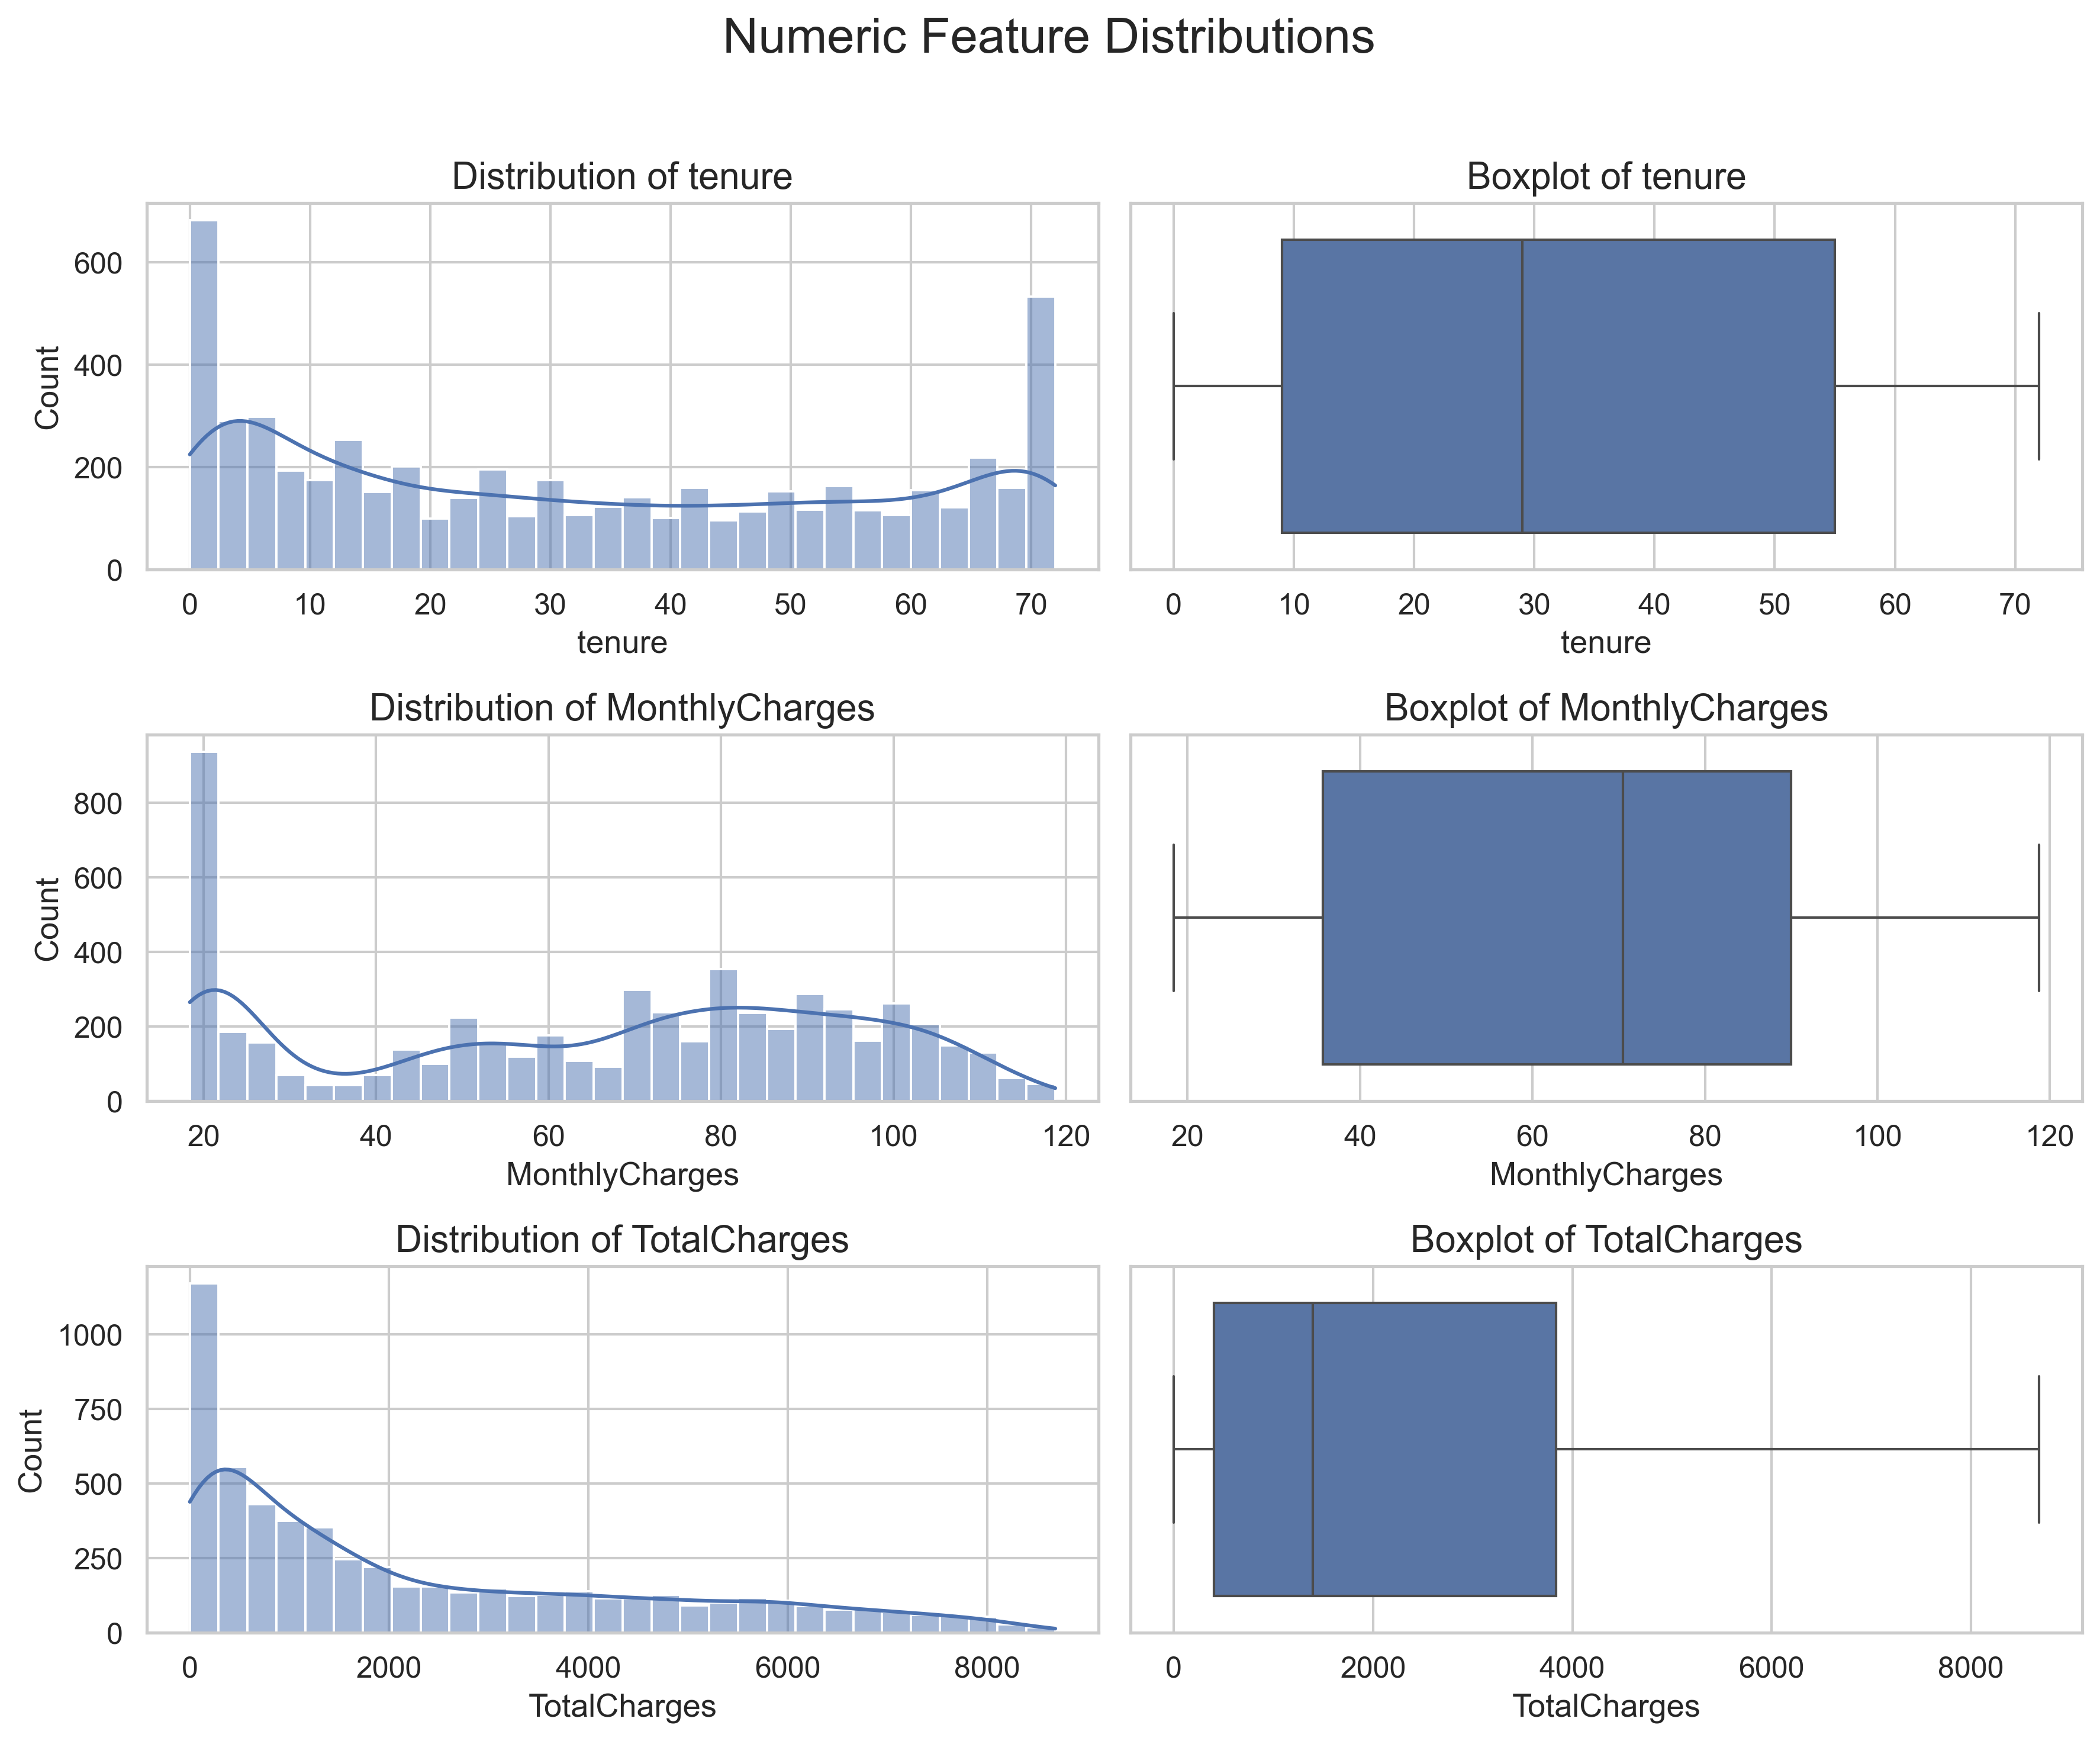
\includegraphics[width=\textwidth]{../figures/training_numeric_feature_distributions.png}
\caption{Numeric feature distributions and boxplots}
\label{fig:training-numeric-distributions}
\end{figure}

The distribution of \texttt{tenure} has substantial mass near low values and also many observations near the upper end of the observed range. This indicates that the training set contains both newly joined customers and long-tenure customers.

The distribution of \texttt{MonthlyCharges} is not symmetric. There is a large group of customers with relatively low monthly charges and a broad group at higher monthly charge levels. The distribution of \texttt{TotalCharges} is strongly right-skewed. This is expected because total charges accumulate over time: many customers have low accumulated charges, while long-tenure or high-monthly-charge customers can have much larger accumulated totals.

These plots are descriptive. They do not justify automatic outlier removal. The raw audit already checked for impossible negative numeric values. High but plausible values should be treated as potential natural observations unless there is separate evidence that they are coding errors.

\subsection{Numeric feature distributions by churn}

Figure \ref{fig:training-numeric-by-churn} compares the numeric feature distributions between churners and non-churners.

\begin{figure}[H]
\centering
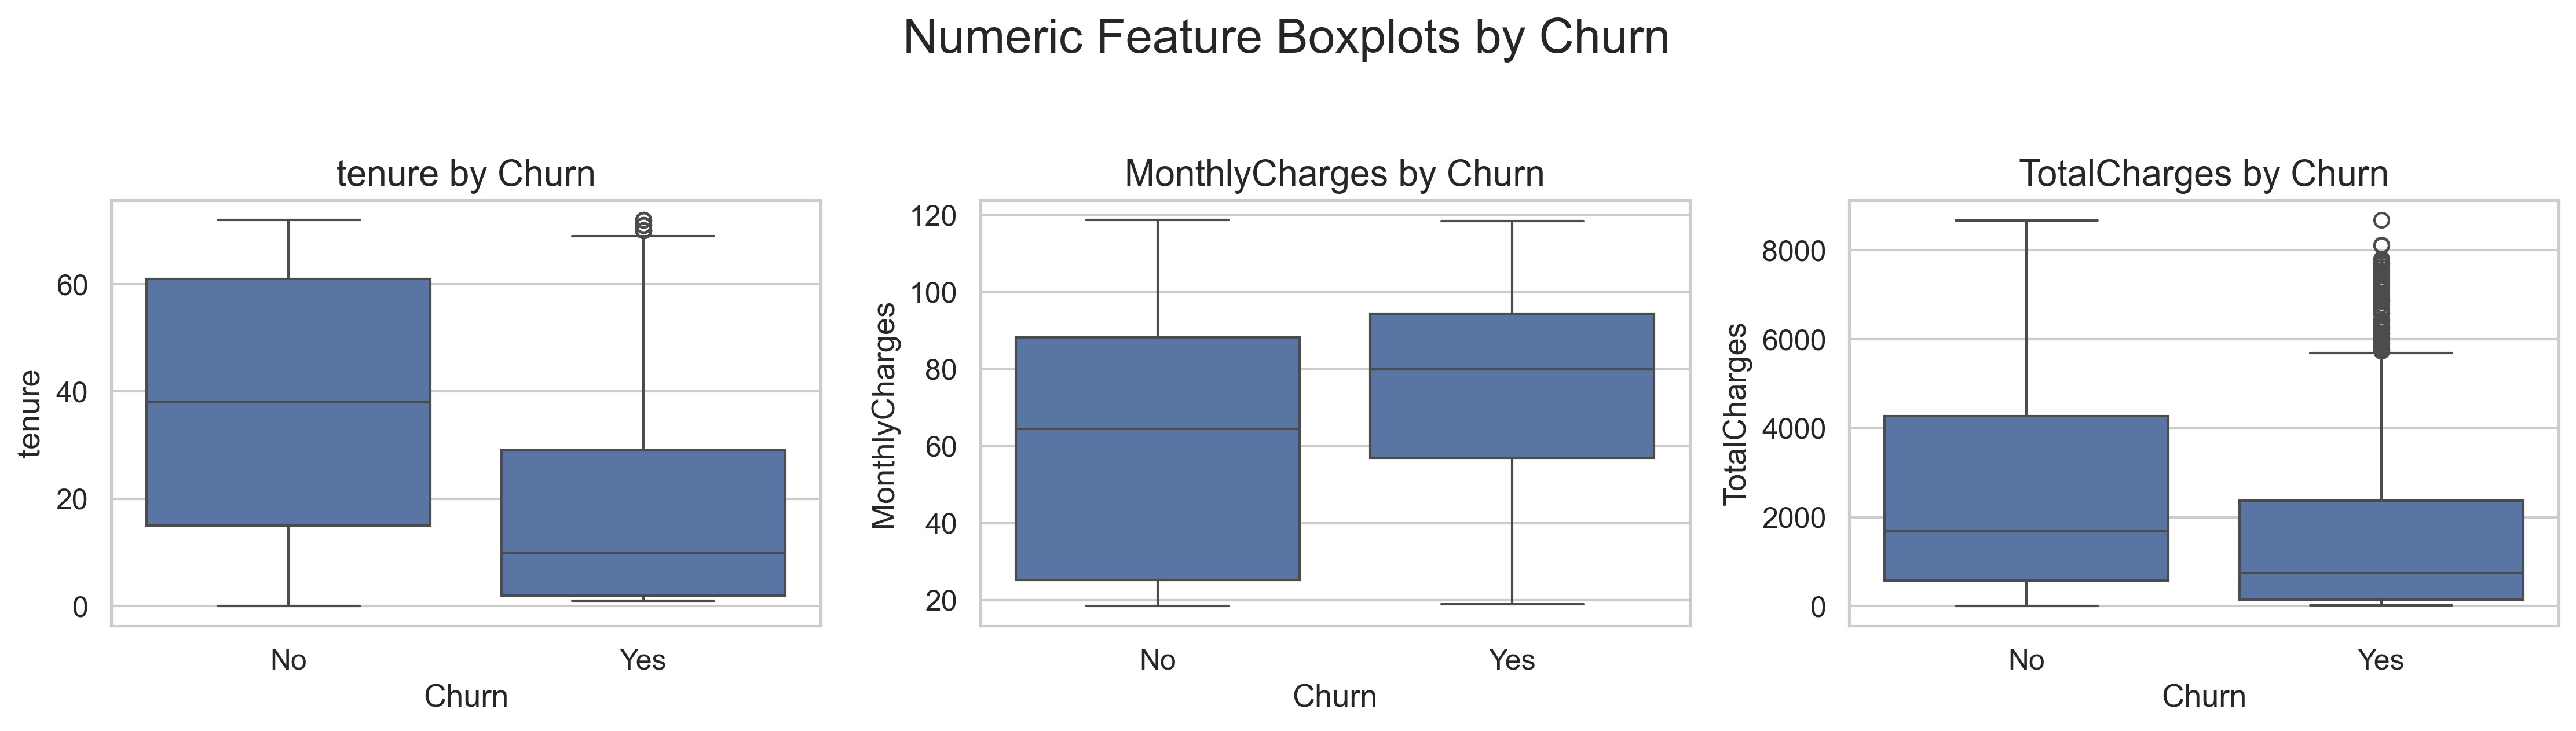
\includegraphics[width=\textwidth]{../figures/training_numeric_feature_boxplots_by_churn.png}
\caption{Numeric feature boxplots by churn}
\label{fig:training-numeric-by-churn}
\end{figure}

The class-conditioned boxplots show clearer feature-target structure than the marginal distributions. Customers who churned have substantially lower \texttt{tenure} than customers who did not churn. This is one of the strongest numeric patterns in the training data and suggests that newer customers are more likely to leave.

\texttt{MonthlyCharges} tends to be higher for churners. This indicates that customers with higher monthly bills may be at greater churn risk, at least as a marginal training-set association. \texttt{TotalCharges} tends to be lower for churners, but this should be interpreted carefully. Since \texttt{TotalCharges} accumulates over time, lower total charges among churners are consistent with churners having shorter tenure.

\subsection{Numeric scatter matrix}

Figure \ref{fig:training-scatter-matrix} shows a scatter matrix for the numeric features, coloured by churn status.

\begin{figure}[H]
\centering
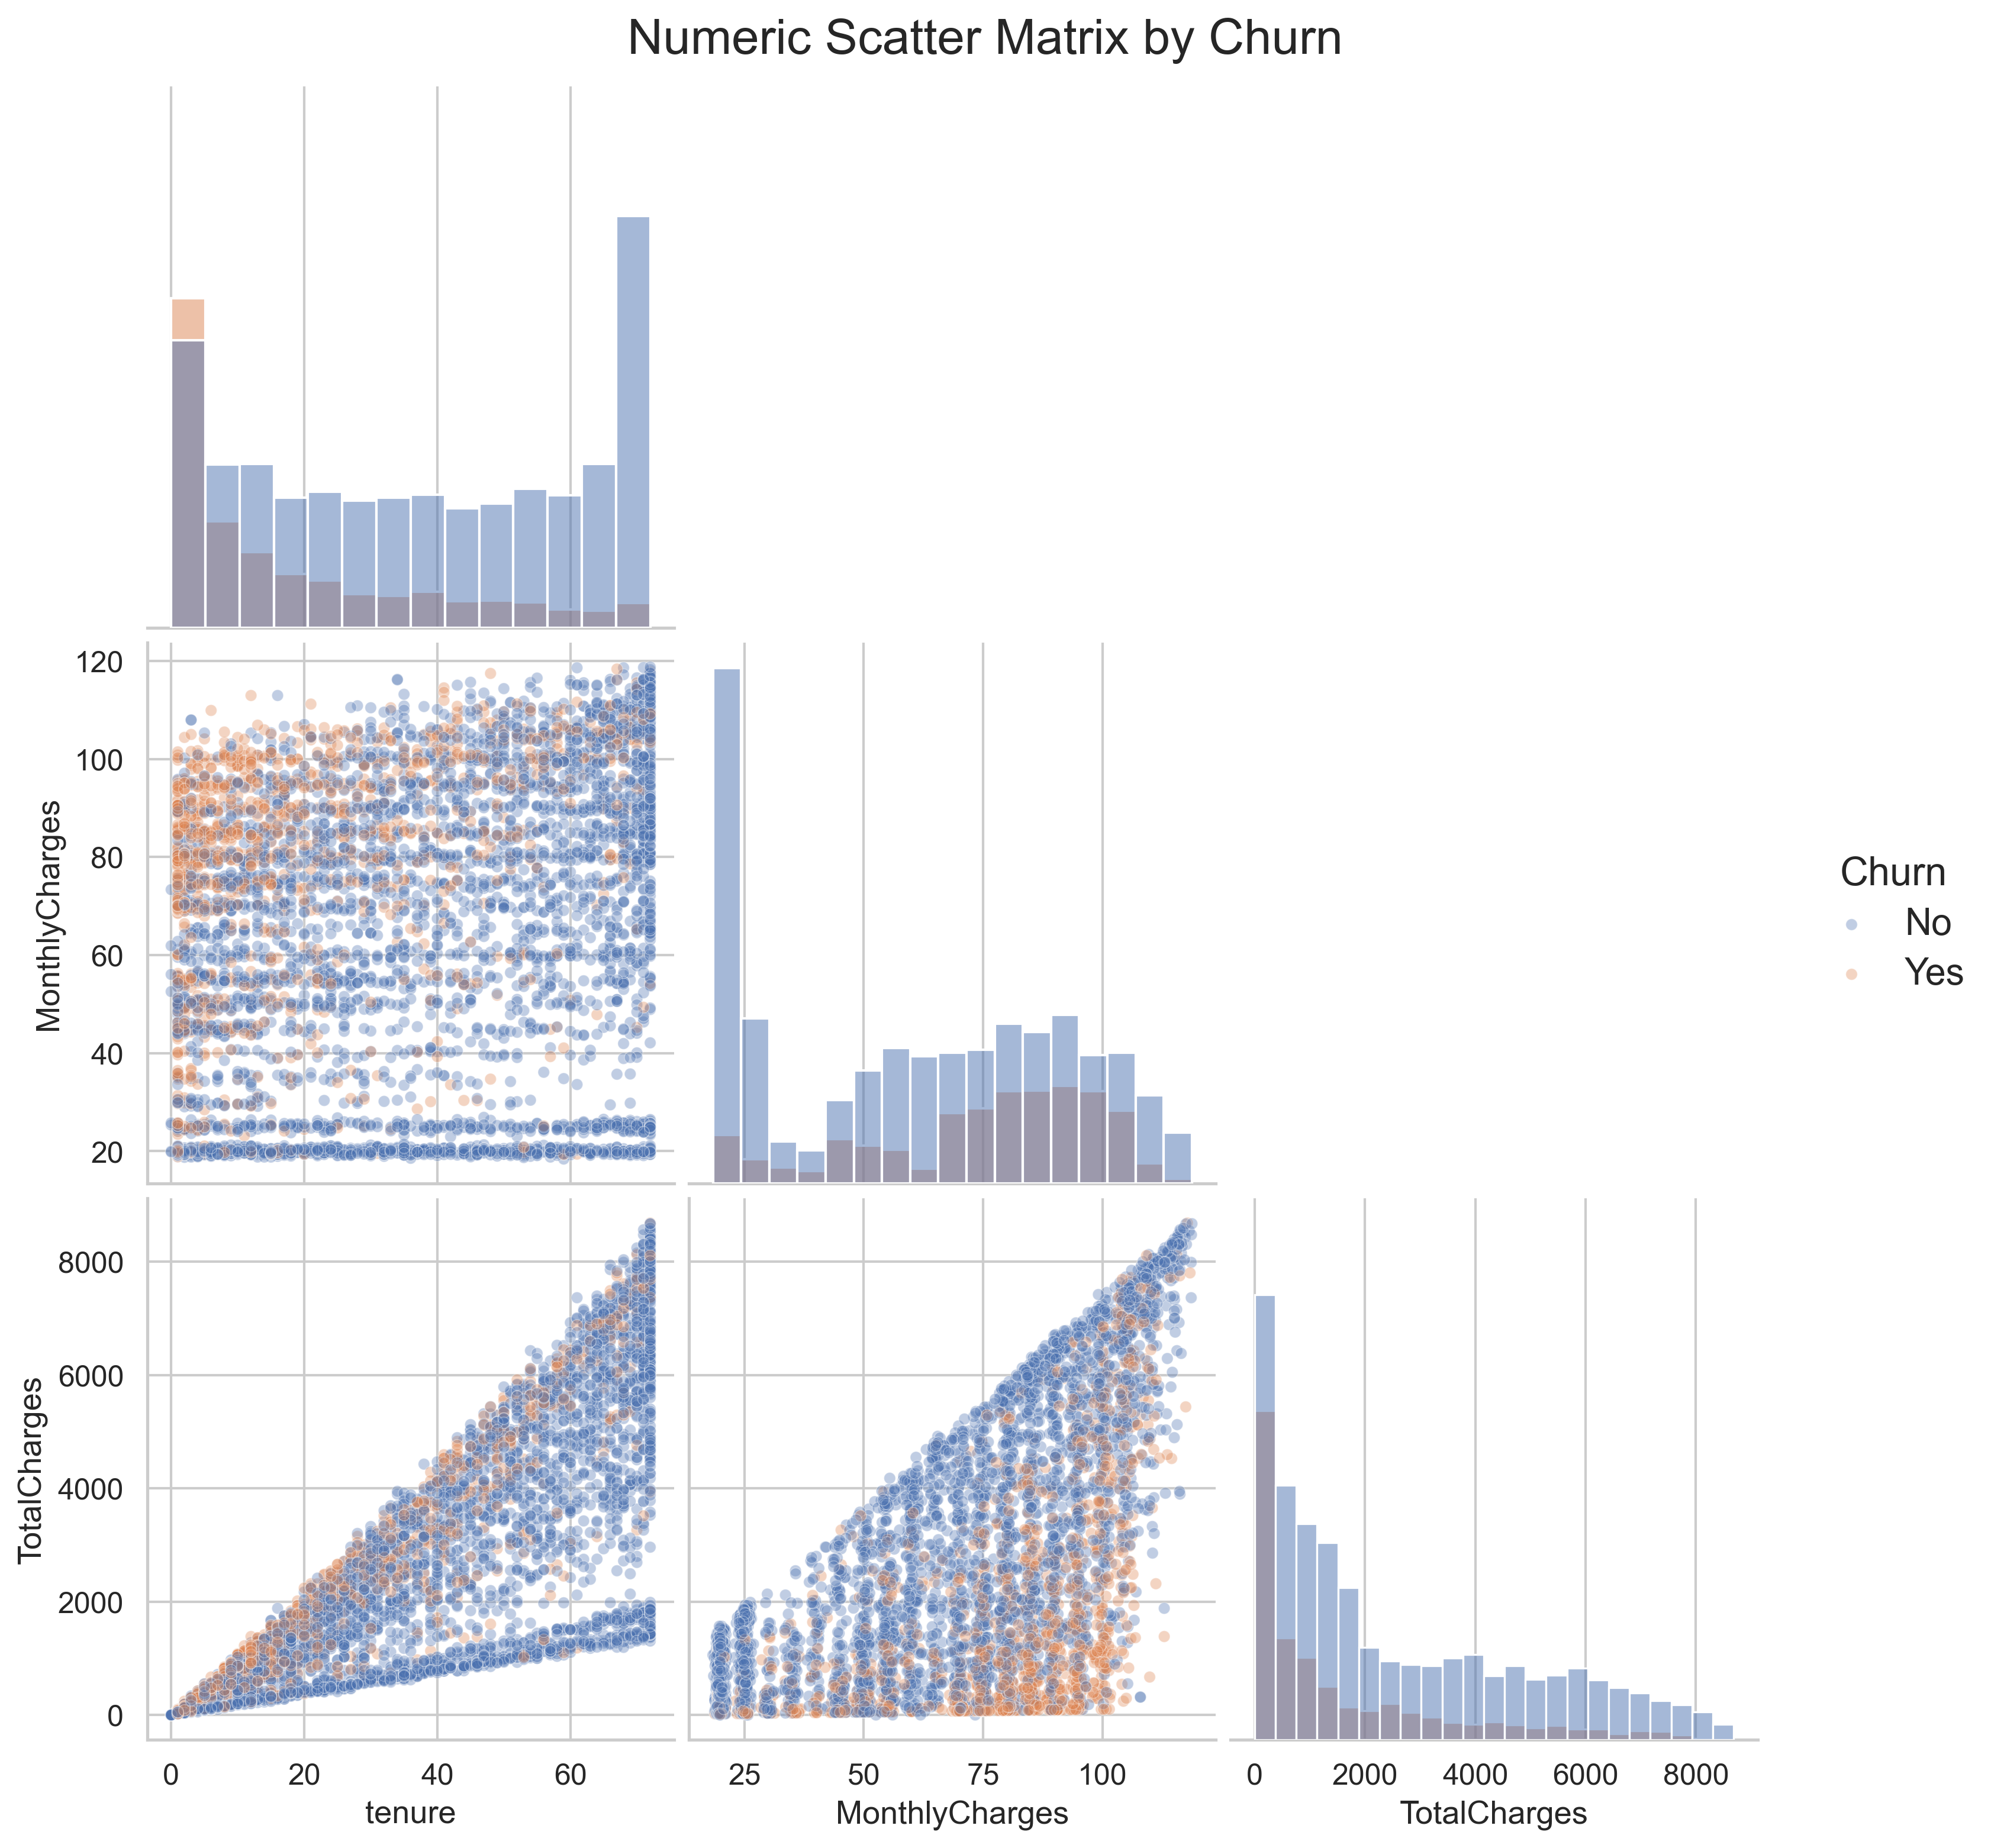
\includegraphics[width=0.88\textwidth]{../figures/training_numeric_scatter_matrix_by_churn.png}
\caption{Numeric scatter matrix by churn}
\label{fig:training-scatter-matrix}
\end{figure}

The scatter matrix shows visible churn-related patterns, but it does not show a clean visual separation between churners and non-churners using any single pair of numeric variables. Churners are more concentrated among customers with shorter tenure and are also relatively visible among customers with higher monthly charges. However, the two classes overlap substantially across the numeric feature space, suggesting that churn is not separable by a simple pairwise numeric boundary.

The clearest structural pattern is the relationship between \texttt{tenure} and \texttt{TotalCharges}. The triangular shape is expected because total charges accumulate over months and are also affected by monthly charges. For a fixed tenure, customers with higher monthly charges can accumulate higher total charges. This motivates using models that can combine numeric and categorical information, and possibly models that can learn interactions.

\subsection{Numeric correlation matrix}

Figure \ref{fig:training-numeric-correlation} shows the Pearson correlation matrix among numeric features and \texttt{Churn\_binary} in this split.

\begin{figure}[H]
\centering
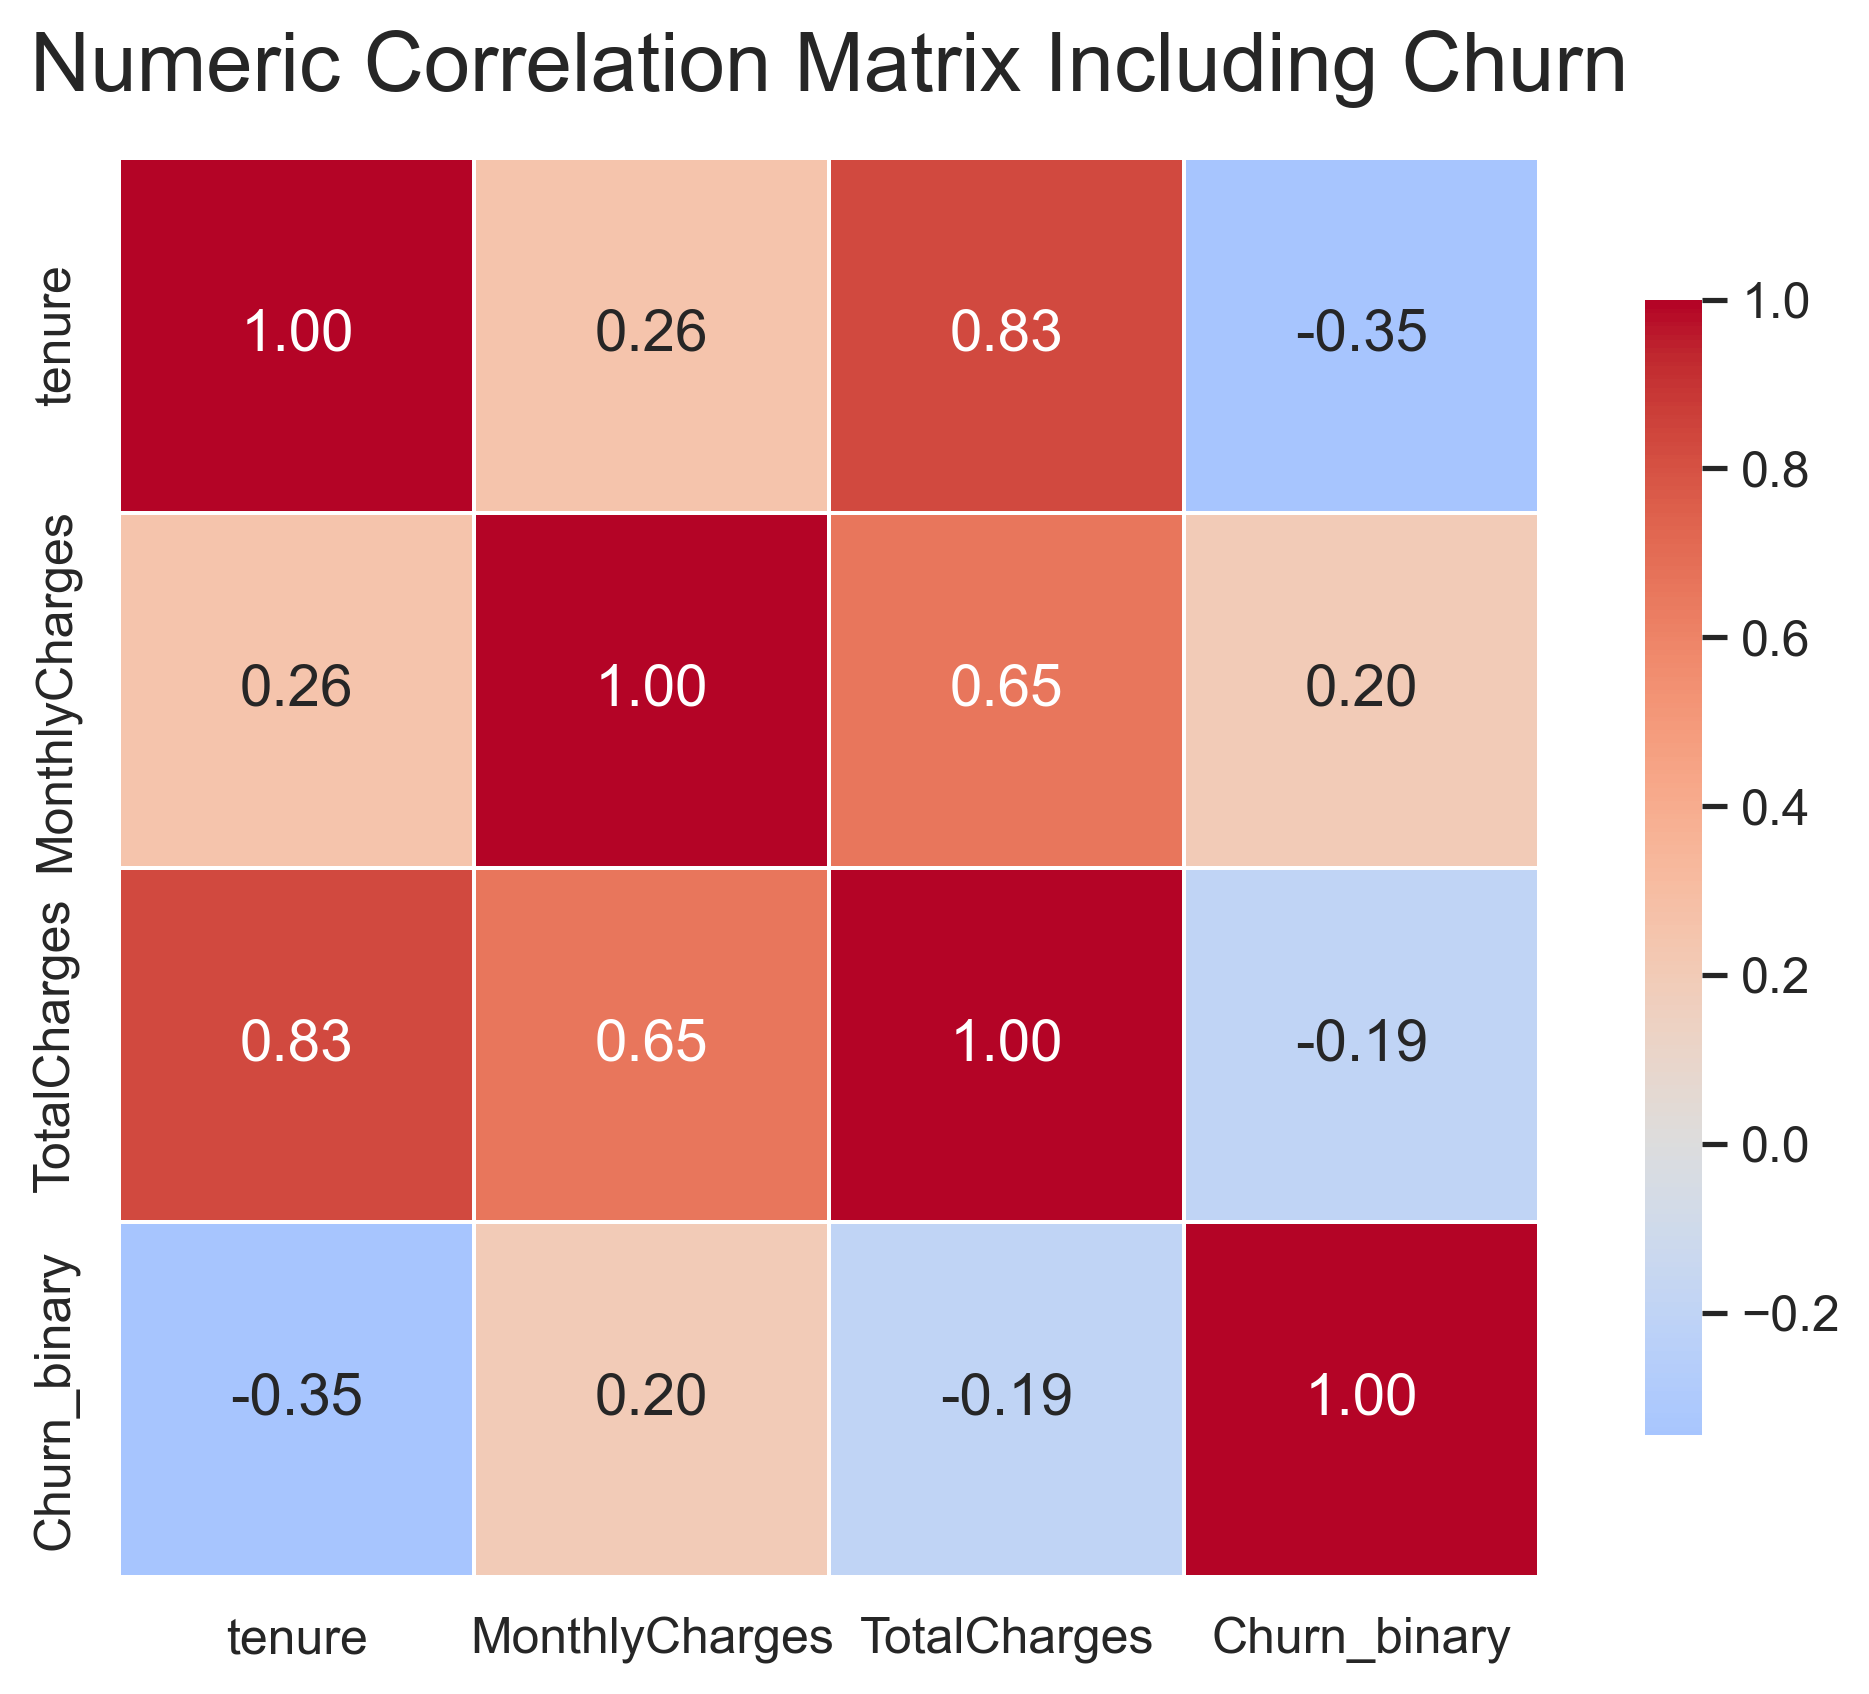
\includegraphics[width=0.55\textwidth]{../figures/training_numeric_correlation_matrix.png}
\caption{Numeric correlation matrix including \texttt{Churn\_binary}}
\label{fig:training-numeric-correlation}
\end{figure}

The strongest numeric correlation with churn is for \texttt{tenure}, with correlation approximately \(-0.35\). Longer-tenure customers are less likely to churn in the training data. \texttt{MonthlyCharges} has a positive correlation with churn of approximately \(0.20\), while \texttt{TotalCharges} has a negative correlation with churn of approximately \(-0.19\).

The correlation matrix also shows that \texttt{tenure} and \texttt{TotalCharges} are strongly correlated, approximately \(0.83\), and that \texttt{MonthlyCharges} and \texttt{TotalCharges} are also positively correlated, approximately \(0.65\). These are marginal linear associations only. They do not capture nonlinear relationships, interactions, or the effects of categorical variables.

\subsection{Categorical feature frequencies}

Figures \ref{fig:training-categorical-frequencies-part-1} and \ref{fig:training-categorical-frequencies-part-2} show the distribution of categorical feature levels. The categorical variables are split across two figures to keep axis labels and category names readable in the compiled report.

\begin{figure}[H]
\centering
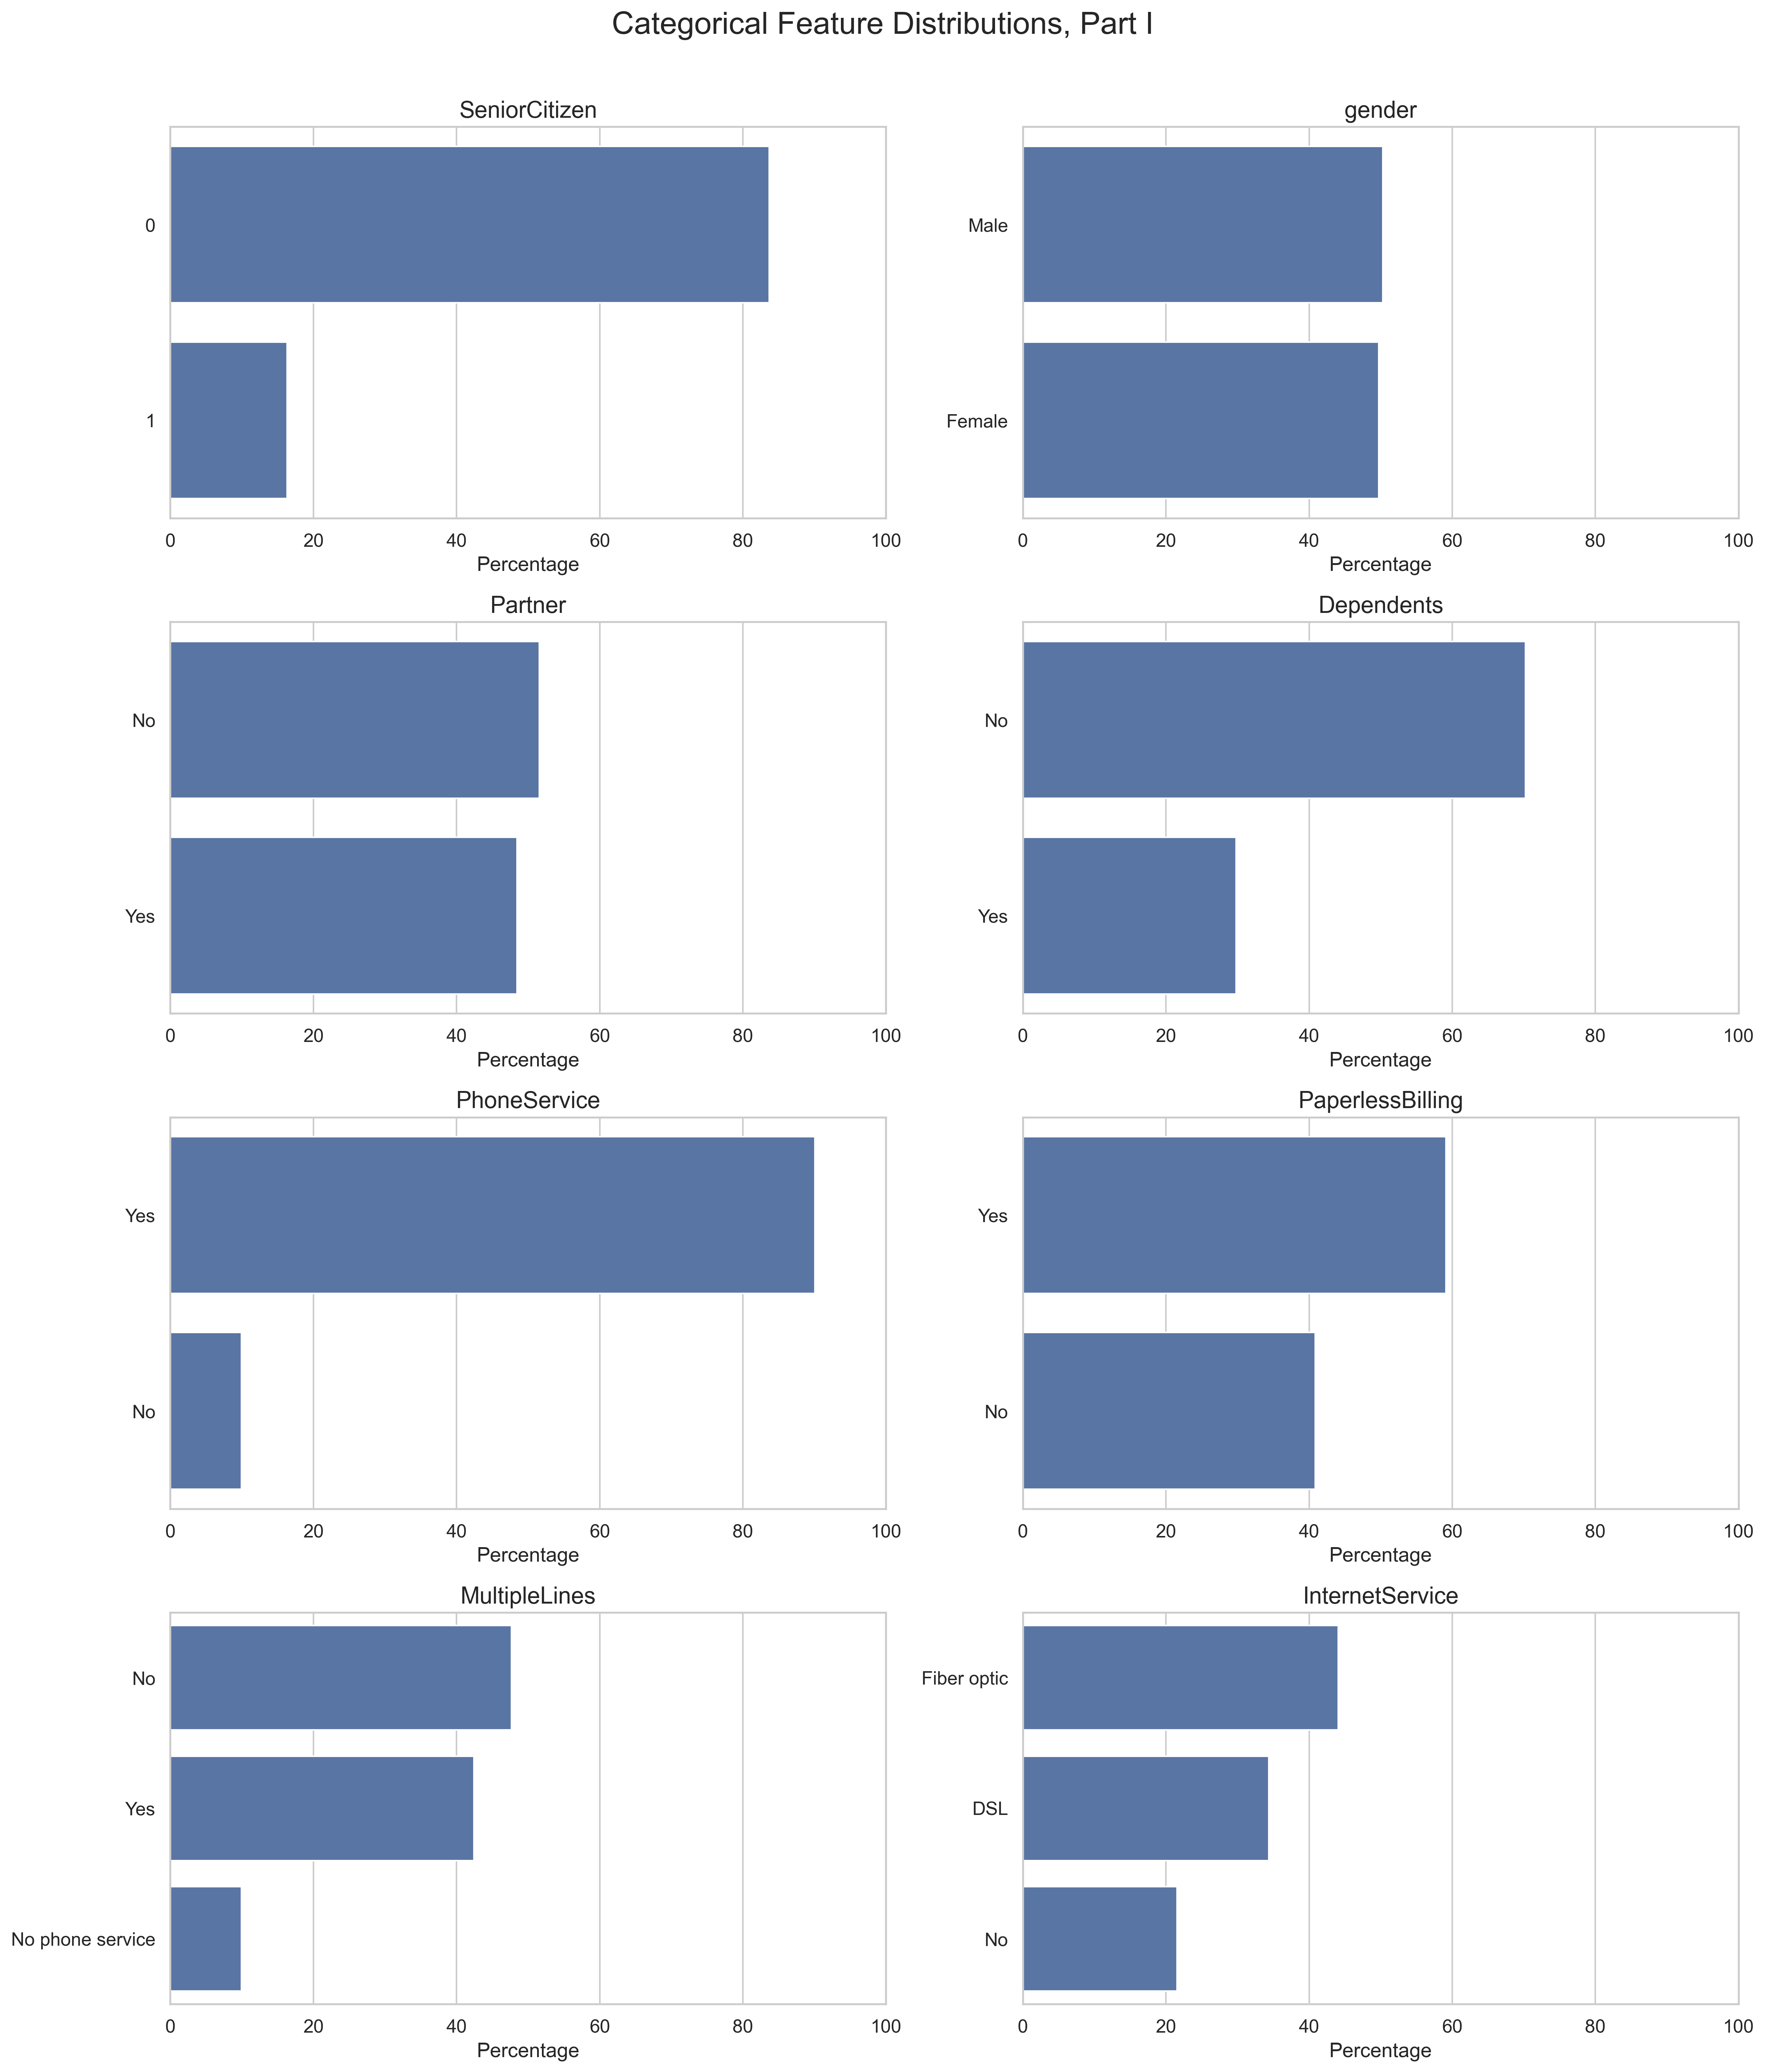
\includegraphics[width=\textwidth]{../figures/training_categorical_feature_frequencies_part_1.png}
\caption{Categorical feature distributions, Part I}
\label{fig:training-categorical-frequencies-part-1}
\end{figure}

\begin{figure}[H]
\centering
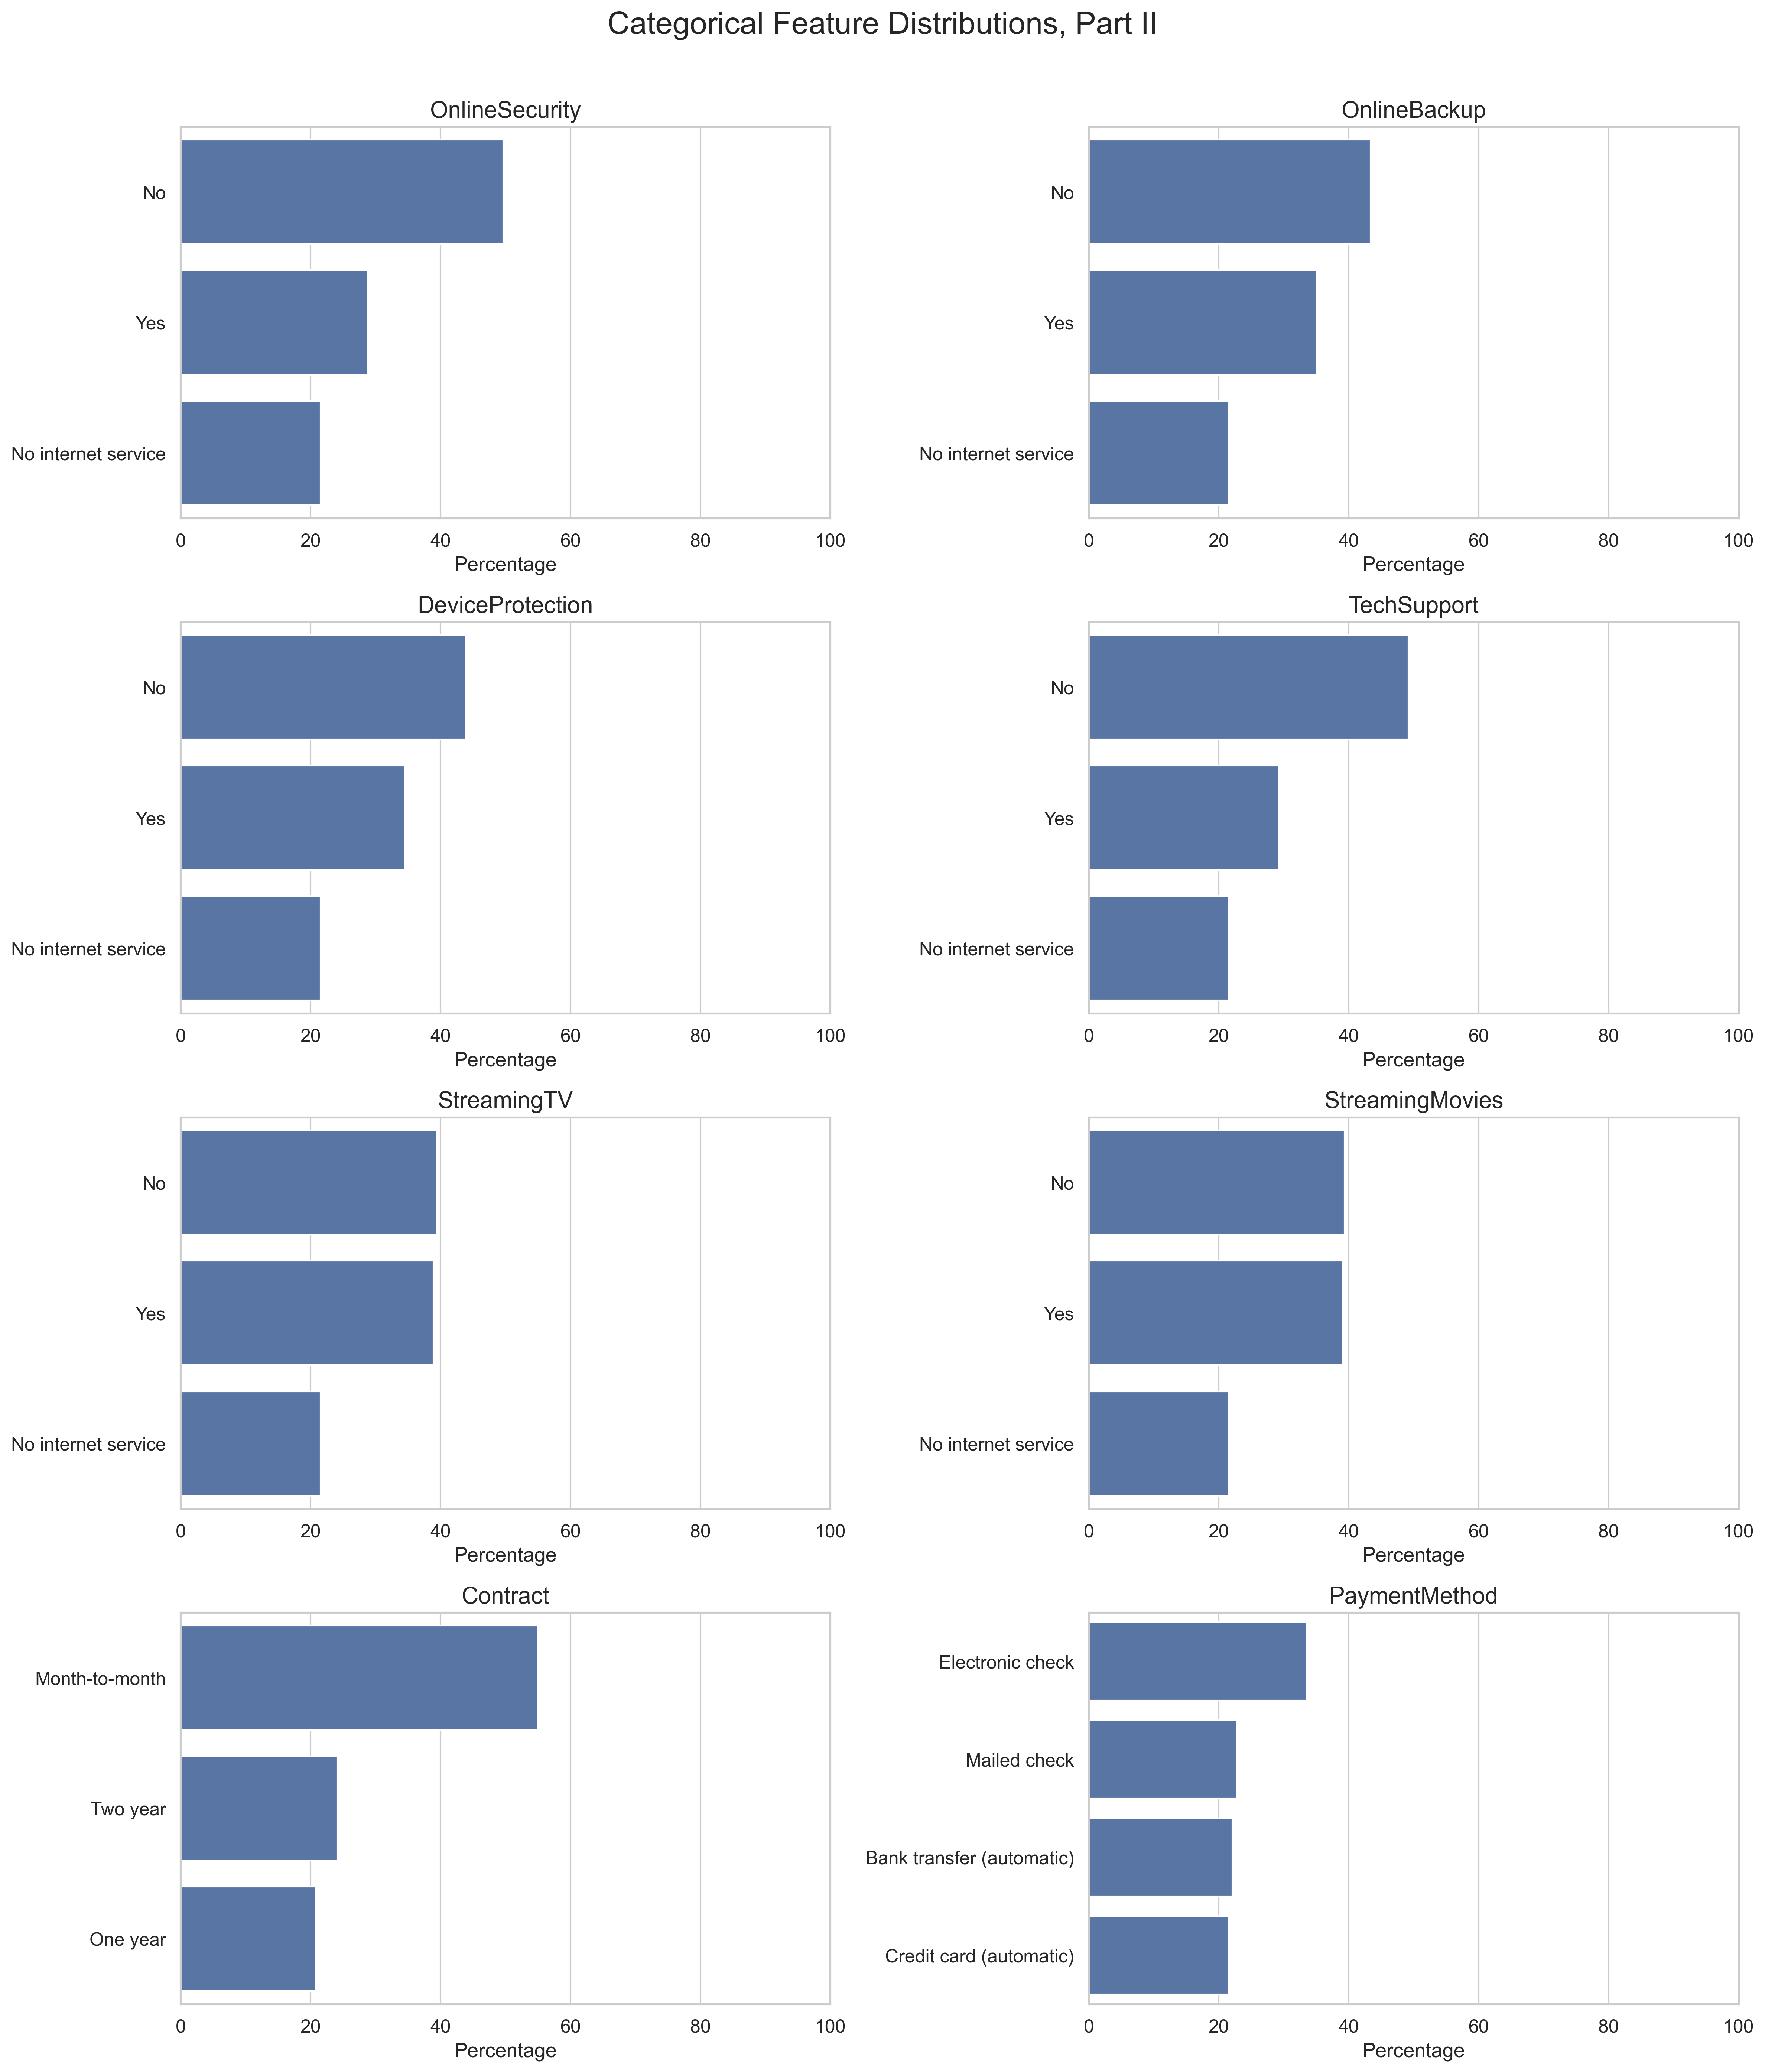
\includegraphics[width=\textwidth]{../figures/training_categorical_feature_frequencies_part_2.png}
\caption{Categorical feature distributions, Part II}
\label{fig:training-categorical-frequencies-part-2}
\end{figure}

Several categorical predictors contain strongly imbalanced levels. For example, \texttt{PhoneService = Yes} represents 90.08\% of the training set, \texttt{SeniorCitizen = 0} represents 83.67\%, and \texttt{Contract = Month-to-month} represents 55.06\%. These imbalances matter because rare levels can create unstable estimates in simple baselines and can affect how much information a model can learn from a category.

Several internet-service add-on variables contain the structural level \texttt{No internet service}. This is not missingness. It is an informative category indicating that the customer does not have internet service. Later preprocessing should preserve this category rather than treating it as a missing value.

\subsection{Categorical churn rates}

Figures \ref{fig:training-categorical-churn-rates-part-1} and \ref{fig:training-categorical-churn-rates-part-2} show the churn rate within each categorical level. Both parts are included in the main section because they support the interpretation: Part I contains demographic, household, billing, phone-service, and internet-service variables, while Part II contains several service add-ons as well as contract type and payment method.

\begin{figure}[H]
\centering
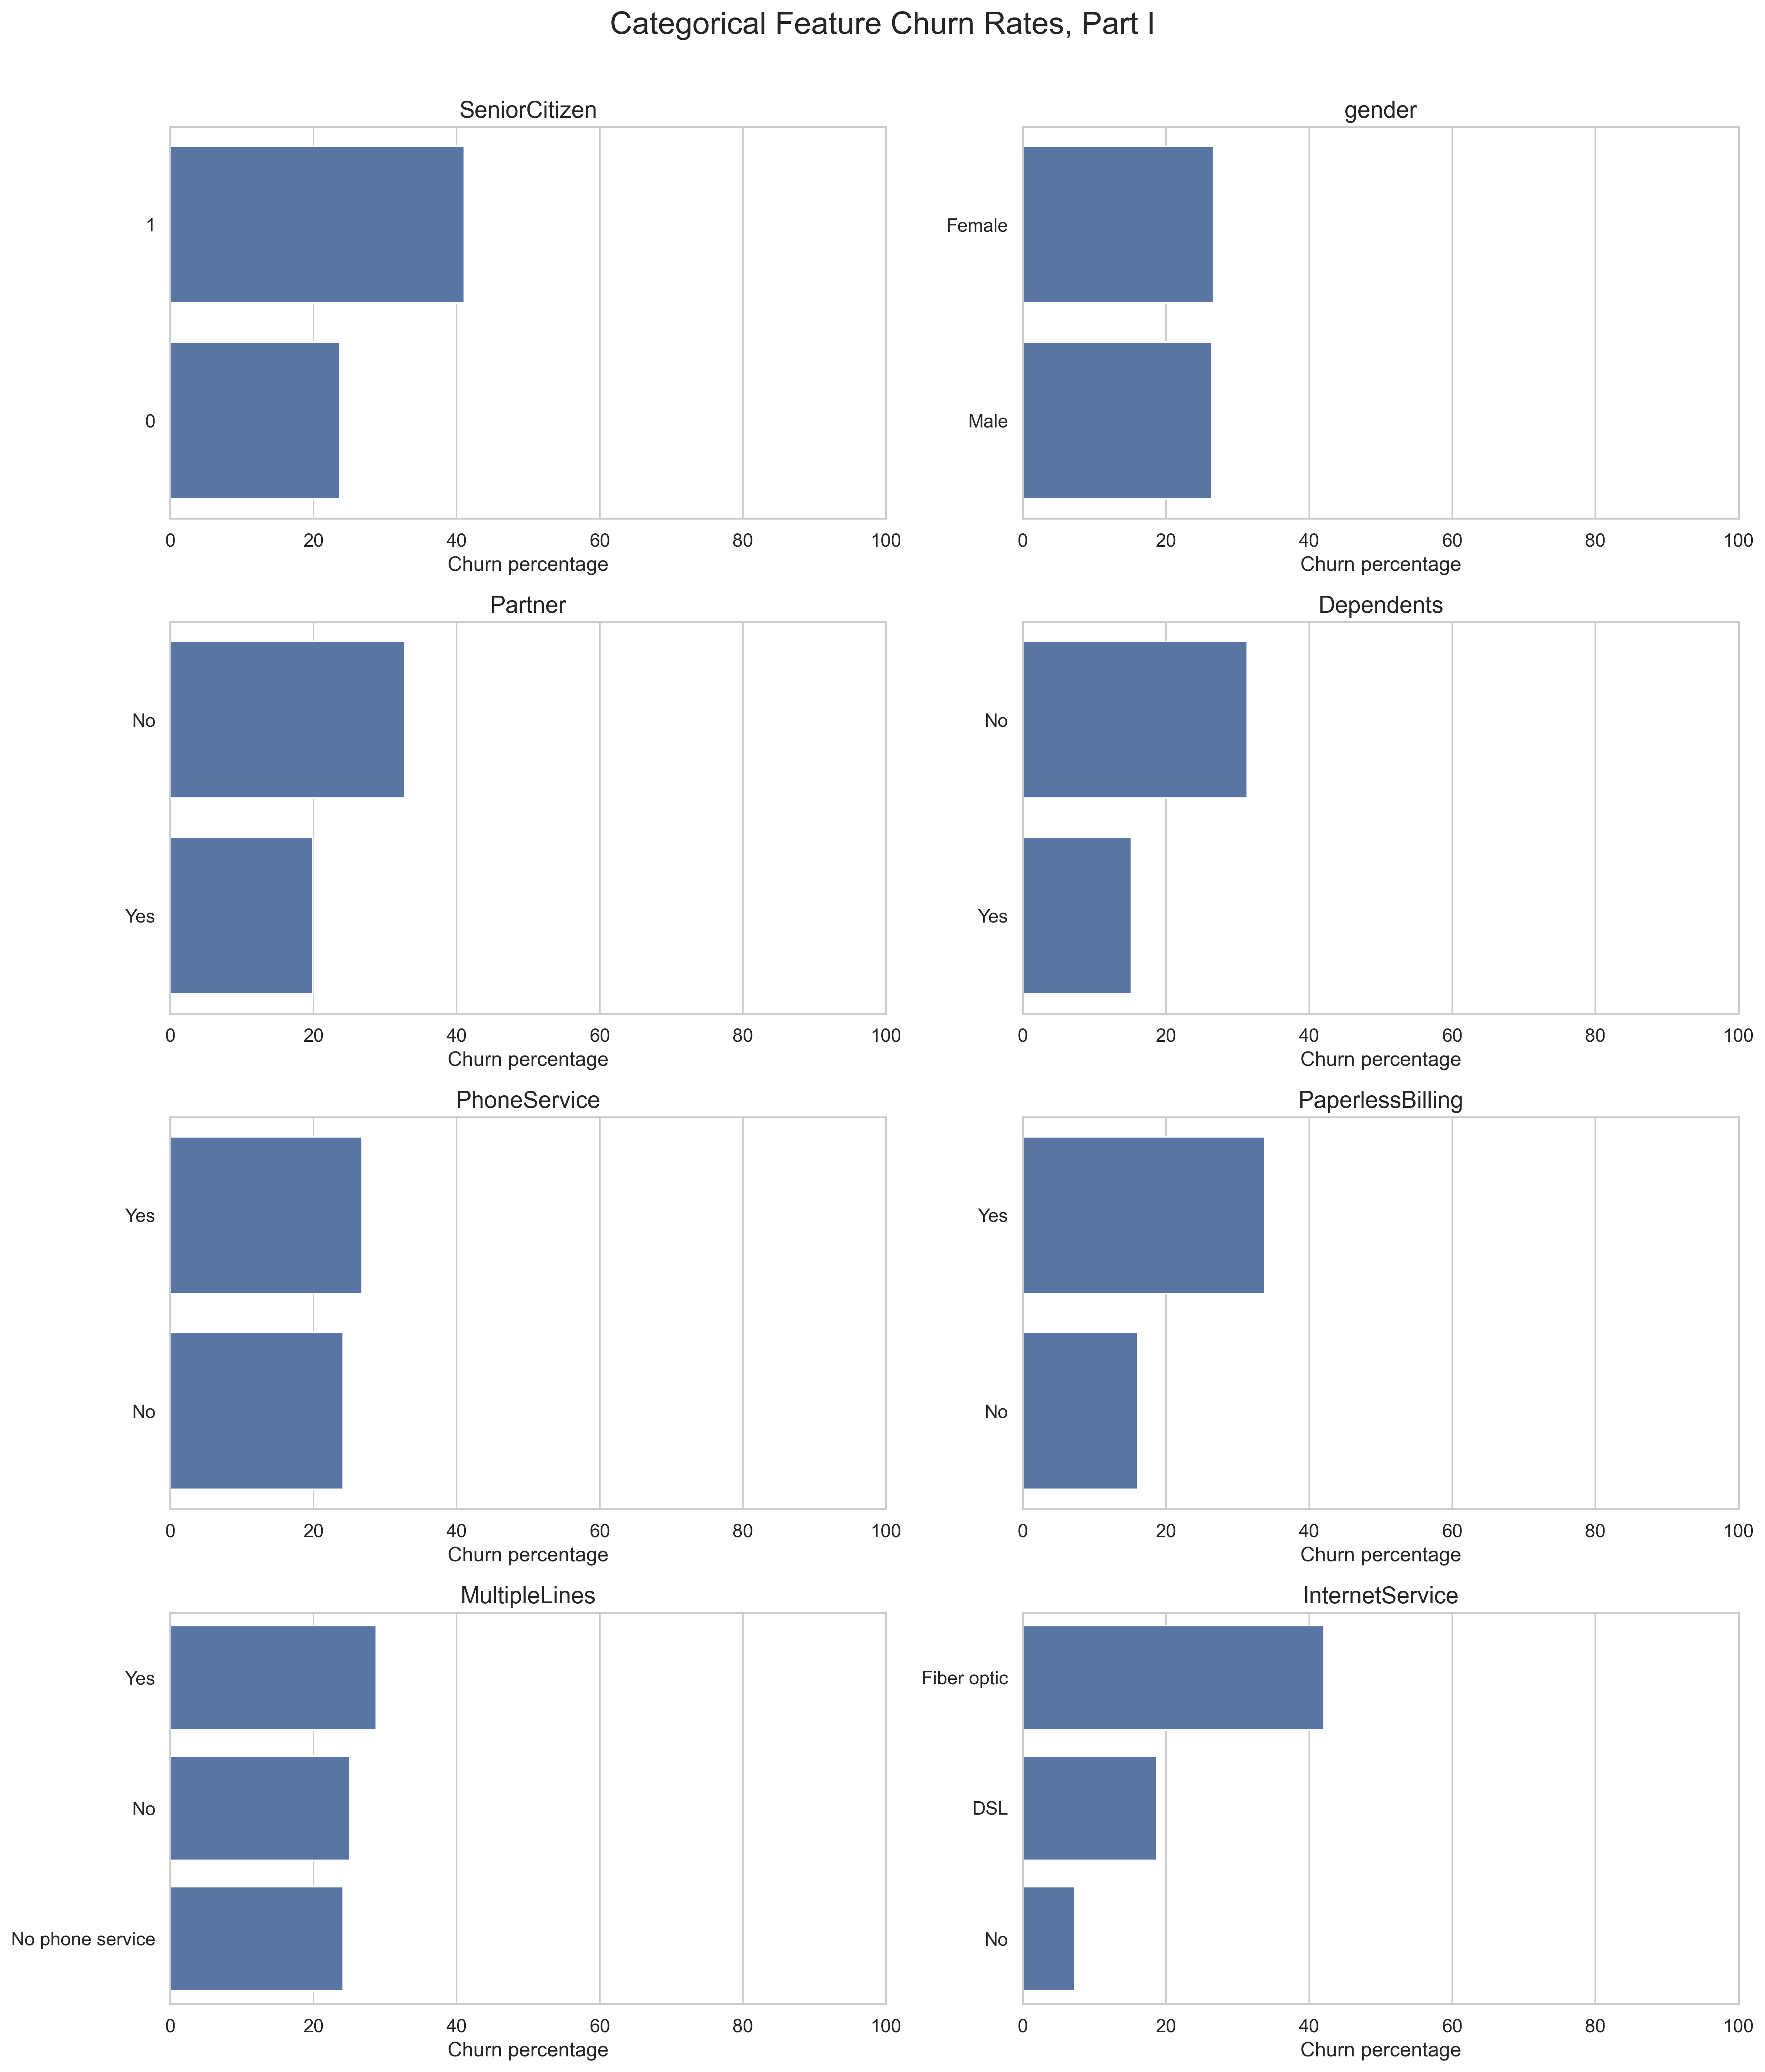
\includegraphics[width=\textwidth]{../figures/training_categorical_feature_churn_rates_part_1.png}
\caption{Categorical feature churn rates, Part I}
\label{fig:training-categorical-churn-rates-part-1}
\end{figure}

\begin{figure}[H]
\centering
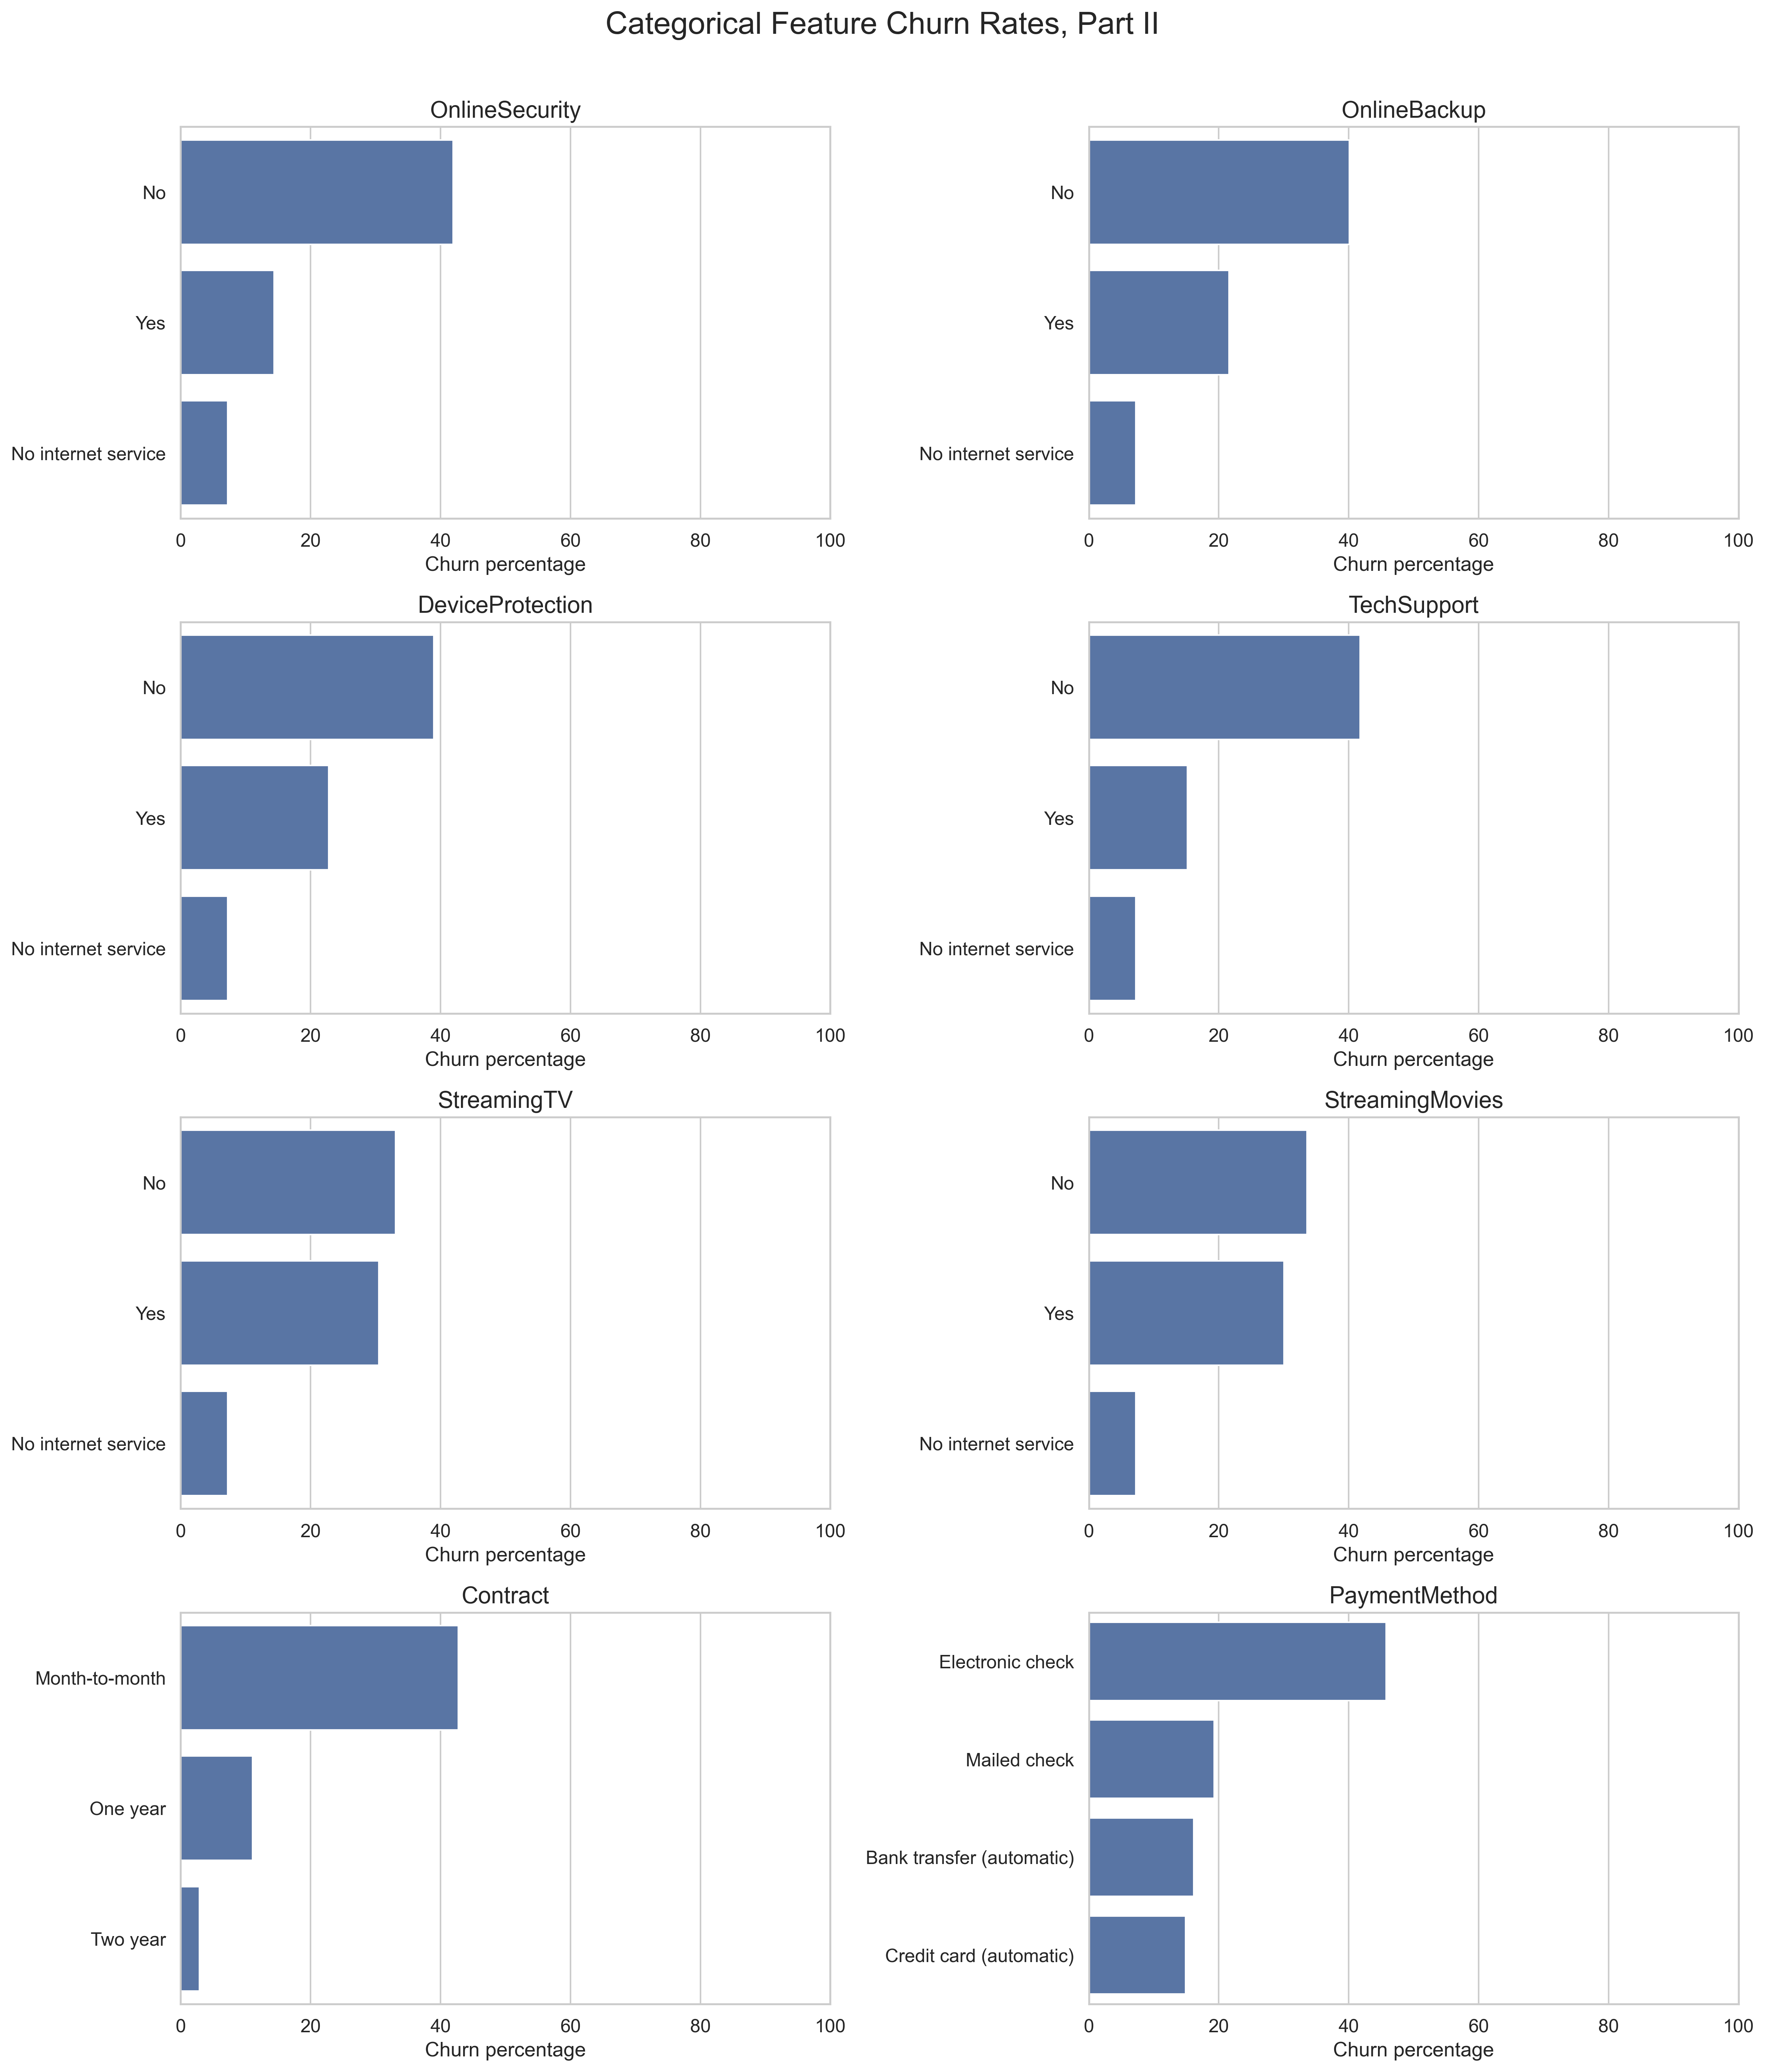
\includegraphics[width=\textwidth]{../figures/training_categorical_feature_churn_rates_part_2.png}
\caption{Categorical feature churn rates, Part II}
\label{fig:training-categorical-churn-rates-part-2}
\end{figure}

The categorical churn-rate plots reveal several large training-set differences. Contract type is one of the strongest categorical patterns: month-to-month customers have a churn rate of 42.75\%, compared with 11.08\% for one-year contracts and 2.87\% for two-year contracts. Internet service type also differs strongly: fiber optic customers have a churn rate of 42.09\%, compared with 18.69\% for DSL and 7.25\% for customers with no internet service.

Payment method is also informative. Customers using electronic check have a churn rate of 45.74\%, higher than mailed check at 19.28\%, bank transfer at 16.16\%, and credit card at 14.92\%. Customers without online security or tech support also show much higher churn rates than customers with those services.

Some variables show weak marginal separation. For example, churn rates for \texttt{gender} are almost identical, and \texttt{PhoneService} shows only a small difference. This does not mean these variables must be removed, because they may still contribute through interactions or in combination with other features. It does suggest that their standalone marginal relationship with churn is weak.

\subsection{Selected categorical churn-rate table}

Table \ref{tab:selected-categorical-churn-rates} reports selected categorical levels that are especially relevant for interpretation and later baseline design.

\begin{table}[H]
\centering
\caption{Selected categorical churn rates}
\label{tab:selected-categorical-churn-rates}
\begin{tabular}{llrrr}
\toprule
Feature & Level & Count & Training \% & Churn \% \\
\midrule
\texttt{Contract} & Month-to-month & 3102 & 55.06 & 42.75 \\
\texttt{Contract} & One year & 1173 & 20.82 & 11.08 \\
\texttt{Contract} & Two year & 1359 & 24.12 & 2.87 \\
\texttt{InternetService} & Fiber optic & 2483 & 44.07 & 42.09 \\
\texttt{InternetService} & DSL & 1937 & 34.38 & 18.69 \\
\texttt{InternetService} & No & 1214 & 21.55 & 7.25 \\
\texttt{PaymentMethod} & Electronic check & 1891 & 33.56 & 45.74 \\
\texttt{PaperlessBilling} & Yes & 3331 & 59.12 & 33.80 \\
\texttt{PaperlessBilling} & No & 2303 & 40.88 & 16.02 \\
\texttt{SeniorCitizen} & 1 & 920 & 16.33 & 41.09 \\
\texttt{SeniorCitizen} & 0 & 4714 & 83.67 & 23.70 \\
\bottomrule
\end{tabular}
\end{table}

These are associations in the training data, not causal effects. They are useful for understanding the dataset, designing simple baselines, and interpreting later models.

\subsection{Summary}

The EDA suggests that the dataset contains meaningful predictive structure. Numerically, churn is most clearly associated with lower tenure and somewhat higher monthly charges. \texttt{TotalCharges} is lower among churners, but this is closely related to the shorter tenure of churned customers.

Categorically, the strongest visible churn-rate differences occur for contract type, internet service type, payment method, online security, tech support, paperless billing, and senior-citizen status. These patterns motivate the next stage: building preprocessing pipelines and baseline classifiers using only the training set.


\newpage
\section{Statistical evaluation methodology}
\label{sec:statistical-evaluation-methodology}

This section defines the statistical interpretation of the model evaluations used throughout the project. It is placed before the learned-model sections because later tables compare multiple model families, hyperparameter settings, thresholds, and ranking metrics. Without a careful evaluation framework, it is easy to overinterpret small differences in cross-validated scores.

The main principle is that a reported metric is an estimate of an unobserved population quantity. A model does not have only a table of observed scores; it has an unknown true generalization performance under the data-generating process. The dataset provides finite-sample estimates of that performance. Therefore, model evaluation is a statistical estimation problem.

\subsection{Data-generating distribution and true performance}

Let \((X,Y)\) denote a customer feature vector and the corresponding churn label. The supervised learning problem can be written as
\[
(X,Y) \sim p(x,y),
\]
where \(p(x,y)\) is the unknown data-generating distribution. The observed dataset is a finite sample,
\[
\mathcal{D}
=
\{(x_i,y_i)\}_{i=1}^{n}.
\]
The goal is not to perform well only on the observed rows, but to perform well on future customers drawn from the same, or sufficiently similar, distribution.

For a fitted classifier \(h\), the true accuracy is
\[
A(h)
=
P(h(X)=Y)
=
\mathbb{E}_{(X,Y)\sim p}
\left[
\mathbb{1}\{h(X)=Y\}
\right].
\]
This quantity is not directly observable because \(p(x,y)\) is unknown. On a finite evaluation sample, it is estimated by
\[
\widehat{A}(h)
=
\frac{1}{n}
\sum_{i=1}^{n}
\mathbb{1}\{h(x_i)=y_i\}.
\]
The same distinction applies to recall, precision, specificity, \(F_1\), ROC-AUC, PR-AUC, calibration metrics, and expected cost. Each reported value is a finite-sample estimate of a population quantity.

This distinction is especially important when comparing models with close observed scores. A difference such as \(0.658\) versus \(0.655\) in PR-AUC is not automatically a meaningful population-level difference. It may reflect real model quality, sampling noise, fold-split randomness, hyperparameter-selection noise, or training randomness.

\subsection{Accuracy as a statistical estimator}

Accuracy has a simple statistical interpretation. For a fixed classifier \(h\), define
\[
Z_i
=
\mathbb{1}\{h(x_i)=y_i\}.
\]
If the evaluation observations are independent draws from the population, then \(Z_i\) can be viewed as a Bernoulli variable with success probability equal to the true accuracy \(A(h)\). The sample accuracy is the average of these Bernoulli variables,
\[
\widehat{A}(h)
=
\frac{1}{n}
\sum_{i=1}^{n} Z_i.
\]
A rough standard error is
\[
\widehat{\mathrm{SE}}(\widehat{A})
=
\sqrt{
\frac{\widehat{A}(1-\widehat{A})}{n}
}.
\]
A normal-approximation 95 percent confidence interval is
\[
\widehat{A}
\pm
1.96
\sqrt{
\frac{\widehat{A}(1-\widehat{A})}{n}
}.
\]
This formula is not the final uncertainty method used for all metrics in this project, but it gives the core intuition: evaluation-set size controls how precisely performance can be estimated.

For example, if an accuracy estimate is \(0.80\) on only \(100\) observations, the rough standard error is
\[
\sqrt{\frac{0.8(0.2)}{100}}=0.04,
\]
so a rough 95 percent interval is approximately
\[
0.80 \pm 1.96(0.04)
=
0.80 \pm 0.078.
\]
That interval is wide. The same point estimate on \(10000\) observations has standard error
\[
\sqrt{\frac{0.8(0.2)}{10000}}=0.004,
\]
which gives a much narrower interval. Thus, evaluation data size can be as important as training data size when the aim is to make precise performance claims.

\subsection{Why other classification metrics need care}

Accuracy is a simple average of correct/incorrect indicators. Other metrics are more complicated. Recall and specificity are class-conditional proportions:
\[
\mathrm{Recall}
=
\frac{TP}{TP+FN},
\qquad
\mathrm{Specificity}
=
\frac{TN}{TN+FP}.
\]
Precision is a proportion among predicted positives:
\[
\mathrm{Precision}
=
\frac{TP}{TP+FP},
\]
where the denominator depends on the model's predictions. The \(F_1\)-score is a nonlinear combination of precision and recall:
\[
F_1
=
\frac{
2\cdot\mathrm{Precision}\cdot\mathrm{Recall}
}{
\mathrm{Precision}+\mathrm{Recall}
}.
\]
ROC-AUC and PR-AUC are ranking metrics computed from score distributions across thresholds. Their sampling uncertainty is not captured by the simple binomial formula for accuracy.

For this reason, final model evaluation should eventually use more general uncertainty tools, especially bootstrap confidence intervals and paired bootstrap intervals for differences between top models. Section-level model comparisons before the final stage should therefore be interpreted as development evidence rather than final statistical proof.

\subsection{Train, validation, and test roles}

The project follows a strict separation between training, validation, and test roles:
\begin{itemize}
    \item training data are used to estimate model parameters;
    \item validation data or cross-validation inside the training set are used to choose preprocessing, features, hyperparameters, thresholds, calibration methods, and model families;
    \item test data are reserved for final performance estimation after all choices are fixed.
\end{itemize}

The held-out test set is not used in the current model sections. This is intentional. If the test set is repeatedly checked during development, it becomes part of the model-selection process and can no longer provide an honest final estimate. Once test-set information has influenced modelling decisions, that mistake cannot be undone without obtaining a new independent test set.

In this project, all section-level model results are computed inside the training set using stratified cross-validation. They are development-stage estimates. Final performance will be evaluated later on the untouched held-out test set after the final model, threshold, and any calibration choices have been fixed.

\subsection{Cross-validation as a development-stage estimator}

In \(K\)-fold cross-validation, the training set is split into \(K\) folds. For fold \(k\), the model is fitted on the other \(K-1\) folds and evaluated on fold \(k\). If \(\widehat{M}^{(k)}\) is the metric on fold \(k\), then the fold-mean cross-validation estimate is
\[
\widehat{M}_{CV}
=
\frac{1}{K}
\sum_{k=1}^{K}
\widehat{M}^{(k)}.
\]
For the churn task, stratified cross-validation is used so that each fold approximately preserves the churn rate. This matters because churn is the minority class.

Cross-validation is useful because it uses the training data efficiently and avoids relying on a single validation split. However, it is still part of model development. When the same cross-validation procedure is used to choose a model or hyperparameter setting, the selected cross-validated score may be mildly optimistic.

\subsection{Fold-mean metrics and pooled out-of-fold metrics}

Two related summaries are used in cross-validation:
\begin{itemize}
    \item fold-mean metrics, where the metric is computed separately on each fold and then averaged;
    \item pooled out-of-fold metrics, where all out-of-fold predictions are collected and one metric is computed on the pooled prediction vector.
\end{itemize}

Pooled out-of-fold predictions are very useful for confusion matrices, threshold curves, ROC curves, precision-recall curves, and calibration plots. However, for nonlinear ranking metrics such as ROC-AUC and PR-AUC, the pooled out-of-fold AUC can differ from the mean of the fold-level AUC values because pooled ranking compares observations whose scores were produced by different fitted models.

The current model sections use pooled out-of-fold predictions for threshold and curve diagnostics. Later, when the project adds a dedicated model-comparison stage, it can store both fold-level and pooled out-of-fold summaries.

\subsection{Hyperparameter tuning and selection optimism}

Hyperparameter tuning changes the interpretation of cross-validation scores. For a fixed modelling setup, cross-validation estimates that setup's development-stage performance. But when many settings are tried and the best score is selected, the selected score is the maximum of several noisy estimates.

For example, suppose a kNN grid tries many values of \(k\), two distance metrics, and two weighting schemes. Some settings may receive slightly lucky validation folds. The best observed configuration is likely to be both good and somewhat lucky. This is selection optimism.

Therefore, when a section says that a configuration is selected, the intended meaning is:
\[
\text{selected within the development grid according to the chosen metric.}
\]
It does not mean:
\[
\text{proven to be uniquely optimal in the population.}
\]
This distinction is especially important when neighbouring hyperparameter settings have very similar scores.

\subsection{Repeated cross-validation}

Repeated cross-validation repeats the fold construction several times with different random splits. For example, repeated 5-fold CV with 10 repeats produces 50 validation scores. This reduces dependence on one particular fold split and can make hyperparameter tuning more stable.

Repeated CV is useful for serious candidate models later in the project, especially if model rankings are close. However, repeated CV does not remove selection optimism completely. If the best setting is selected after many repeated-CV comparisons, the selected score is still the winner among several estimates.

Thus:
\[
\text{repeated CV improves stability,}
\]
whereas
\[
\text{nested CV evaluates a tuning procedure more honestly.}
\]

\subsection{Nested cross-validation}

Nested cross-validation separates tuning from evaluation. It has two loops:
\begin{itemize}
    \item the inner loop chooses hyperparameters using only the outer-training data;
    \item the outer loop evaluates the resulting tuned procedure on held-out outer-validation folds.
\end{itemize}

For each outer fold:
\begin{enumerate}
    \item split the development data into outer-training and outer-validation parts;
    \item run inner cross-validation on the outer-training part to choose hyperparameters;
    \item fit the selected configuration on the full outer-training part;
    \item evaluate once on the outer-validation part.
\end{enumerate}

Nested CV estimates the performance of a procedure, not one fixed hyperparameter setting. For example, a nested-CV estimate for kNN evaluates the procedure ``choose \(k\), distance, and weights by inner CV, then fit kNN with those selected settings.'' Different outer folds may choose different values of \(k\). That is normal because the object being evaluated is the tuning procedure.

Nested CV is useful for comparing tuned model families, such as tuned logistic regression versus tuned kNN versus tuned random forest. The current project does not need nested CV inside every educational model section. Instead, nested CV can be considered later when the strongest model families are compared more formally.

\subsection{Fair hyperparameter-search effort}

Model comparisons can be unfair when one model receives much more tuning effort than another. For example, comparing default logistic regression with a heavily optimized boosting model would partly compare tuning effort rather than model-family quality.

Fair comparison principles include:
\begin{itemize}
    \item use the same training and validation data;
    \item use the same primary selection metric;
    \item use comparable search effort where feasible;
    \item document the search spaces;
    \item avoid tuning the favourite model much more than the baselines;
    \item consider random search, Bayesian optimization, or Optuna-style search when search spaces are large.
\end{itemize}

This does not mean every model family requires identical compute. Some model families have more consequential hyperparameters than others. But the final comparison should be transparent about search effort.

\subsection{Grid search, random search, and adaptive search}

Grid search evaluates every combination from predefined hyperparameter values. It is simple and transparent, but inefficient when the hyperparameter space has many dimensions and only some parameters matter strongly.

Random search samples configurations from predefined distributions. It is often more efficient in high-dimensional spaces because it explores more distinct values of the important dimensions for the same number of trials.

Adaptive methods such as Bayesian optimization or Optuna-style search use earlier trials to decide which configurations to try next. They can be useful for expensive model families, but they are less transparent and add another layer of procedure choice. For this project, simple grids are suitable for early educational sections. More advanced search may be introduced later for final candidate models.

\subsection{Threshold selection as model selection}

Many classifiers output scores or probabilities. A threshold turns a score into a hard prediction:
\[
\hat{y}_{\tau}
=
\mathbb{1}\{s(x)\geq \tau\}.
\]
Changing \(\tau\) changes recall, precision, specificity, \(F_1\), predicted positive rate, and expected cost. Therefore, threshold choice is a model-selection decision.

Threshold curves in the model sections are diagnostic. They show how a model behaves across operating points. The final threshold should be chosen later using training/validation information only, then frozen before the test set is evaluated.

\subsection{Calibration as a separate evaluation dimension}

Ranking performance and probability calibration are different. ROC-AUC and PR-AUC measure whether the model ranks churners above non-churners. Calibration asks whether predicted probabilities are numerically reliable. A model can rank customers well but still produce overconfident or underconfident probabilities.

Calibration matters if predicted probabilities are interpreted as churn risks or used in cost-based decision rules. If calibration is applied later, the calibrator must also be fitted without test leakage, using validation data or a cross-validation-based calibration procedure.

\subsection{Statistical tests and uncertainty methods}

The final project can use several uncertainty tools, each answering a different question:
\begin{itemize}
    \item bootstrap confidence intervals estimate uncertainty around final test metrics;
    \item paired bootstrap intervals compare metric differences between two models on the same test observations;
    \item McNemar's test compares paired hard-classification errors;
    \item DeLong-style tests compare paired ROC-AUCs;
    \item permutation tests can assess whether model performance is stronger than expected under random label association;
    \item repeated CV and nested CV can describe robustness and procedure-level performance before final test evaluation.
\end{itemize}

Bootstrap is especially useful because it can be applied to many metrics, including PR-AUC, ROC-AUC, \(F_1\), recall, precision, balanced accuracy, Brier score, and expected cost. In the final test stage, the project should report point estimates together with uncertainty intervals wherever feasible.

\subsection{Implications for the current report}

The model sections that follow should be read as model-development sections. They explain model families and use training-set cross-validation to compare configurations. Their selected models are representative strong candidates within the tried development grids. They are not final claims of statistical superiority.

The report therefore uses the following interpretation:
\begin{itemize}
    \item large differences are treated as useful development evidence;
    \item small differences between neighbouring hyperparameters are interpreted cautiously;
    \item selected configurations are described as selected within a development grid;
    \item threshold results are diagnostic rather than final operating rules;
    \item final model-family comparison, threshold selection, calibration decisions, and test-set performance are deferred to later stages.
\end{itemize}

This discipline lets the project remain both educational and statistically careful. The individual sections can explain each model in depth, while the final model comparison stage can later use repeated CV, nested CV, bootstrap confidence intervals, paired comparisons, and ablation studies to support stronger final conclusions.


\newpage
\section{Preprocessing, evaluation, and simple baselines}
\label{sec:preprocessing-evaluation-simple-baselines}

\subsection{Purpose of this stage}

This section starts the modelling workflow after the raw-data audit, deterministic correction, train/test split, and training-set exploratory analysis. The purpose is not yet to fit flexible learned models. Instead, this stage establishes the evaluation language and simple reference baselines that all later models must improve upon.

The held-out test set remains unused. All results in this section are computed only from the training set using stratified cross-validation. This preserves the final test set for the final evaluation stage.

The section has three goals. First, it defines the binary classification evaluation framework used throughout the rest of the project. Second, it introduces reusable preprocessing infrastructure for later models. Third, it evaluates simple baselines that do not learn a flexible relationship from the full feature matrix.

The simple baselines considered here are:
\begin{enumerate}
    \item a majority-class baseline;
    \item a prior-probability baseline;
    \item a stratified random baseline;
    \item a uniform random baseline;
    \item an exploratory-analysis-inspired rule baseline.
\end{enumerate}

Learned models such as least-squares classification, logistic regression, k-nearest neighbours, Naive Bayes, decision trees, support vector machines, and neural networks are introduced in later sections.

\subsection{Training-only evaluation discipline}

Let the training set be
\[
\mathcal{D}_{train}
=
\{(x_i,y_i)\}_{i=1}^{n},
\]
where \(x_i\) denotes the feature vector for customer \(i\), and \(y_i \in \{0,1\}\) denotes the binary churn label. In this project, the positive class is churn:
\[
y_i = 1 \quad \Longleftrightarrow \quad \text{customer } i \text{ churned}.
\]

All model-development decisions must be made without using the held-out test set. This includes preprocessing design, feature engineering, feature selection, model-family choice, hyperparameter tuning, threshold tuning, calibration decisions, and model comparison.

For this stage, performance is estimated using stratified 5-fold cross-validation inside the training set. Stratification preserves approximately the same churn rate in each fold. This is important because churn is the minority class. In the training set, the class distribution is shown in Table~\ref{tab:stage04-target-distribution}.

\begin{table}[H]
\centering
\caption{Training-set target distribution.}
\label{tab:stage04-target-distribution}
\begin{tabular}{lrr}
\toprule
Class & Count & Percentage \\
\midrule
No churn (\(Y=0\)) & 4139 & 73.46\% \\
Churn (\(Y=1\)) & 1495 & 26.54\% \\
\bottomrule
\end{tabular}
\end{table}

Cross-validation produces out-of-fold predictions. This means that the prediction for each observation is generated by a model that was not fitted on that same observation. This gives a more honest development-stage estimate than evaluating a model on the same data used to fit it.

\subsection{Positive and negative classes}

Many binary classification metrics are defined relative to the positive class. The positive class is not necessarily the most common class. It is the event of interest.

A medical screening example makes the terminology intuitive. Suppose a test predicts whether a person has cancer. Then:
\begin{itemize}
    \item positive class: the person has cancer;
    \item negative class: the person does not have cancer;
    \item predicted positive: the test says cancer;
    \item predicted negative: the test says no cancer.
\end{itemize}

For the churn problem, the same logic becomes:
\begin{itemize}
    \item positive class: the customer churns;
    \item negative class: the customer does not churn;
    \item predicted positive: the model flags the customer as likely to churn;
    \item predicted negative: the model does not flag the customer as likely to churn.
\end{itemize}

This convention matters because recall, precision, \(F_1\), ROC-AUC, and PR-AUC all depend on which class is treated as positive.

\subsection{Confusion matrix}

The confusion matrix counts the four possible combinations of actual class and predicted class. The positive-first layout used here is shown in Table~\ref{tab:stage04-generic-confusion-matrix}. Rows represent the actual class and columns represent the predicted class.

\begin{table}[H]
\centering
\caption{Positive-first binary confusion matrix layout.}
\label{tab:stage04-generic-confusion-matrix}
\begin{tabular}{llcc}
\toprule
 & & \multicolumn{2}{c}{Predicted} \\
 & & Positive & Negative \\
\midrule
Actual & Positive & TP & FN \\
Actual & Negative & FP & TN \\
\bottomrule
\end{tabular}
\end{table}

The entries are:
\[
TP = \#\{\hat{y}=1, y=1\},
\qquad
FN = \#\{\hat{y}=0, y=1\},
\]
\[
FP = \#\{\hat{y}=1, y=0\},
\qquad
TN = \#\{\hat{y}=0, y=0\}.
\]

This order is chosen to match the lecture-style visual explanation: actual positives are shown first, and within that row the model can either correctly predict positive or incorrectly predict negative. Some software libraries store confusion matrices in a negative-first numeric order. In the code, the counts are computed with explicit labels and then renamed so that the report can present the matrix in the positive-first order.

In the medical screening example:
\begin{itemize}
    \item true positive: the test says cancer, and the person really has cancer;
    \item false negative: the test says no cancer, but the person really has cancer;
    \item false positive: the test says cancer, but the person does not have cancer;
    \item true negative: the test says no cancer, and the person does not have cancer.
\end{itemize}

In the churn problem:
\begin{itemize}
    \item true positive: the model predicts churn, and the customer churns;
    \item false negative: the model predicts no churn, but the customer churns;
    \item false positive: the model predicts churn, but the customer does not churn;
    \item true negative: the model predicts no churn, and the customer does not churn.
\end{itemize}

False positives and false negatives have different practical meanings. A false positive may lead to unnecessary retention effort for a customer who would have stayed anyway. A false negative may mean missing a customer who actually leaves.

\subsection{Accuracy and the class-imbalance problem}

Accuracy is the fraction of all predictions that are correct:
\[
\text{Accuracy}
=
\frac{TP + TN}{TP + FN + FP + TN}.
\]

Accuracy is intuitive, but it can be misleading when one class is much more common than the other. In this dataset, about \(73.46\%\) of training customers do not churn. A classifier that always predicts no churn can therefore achieve \(73.46\%\) accuracy while detecting zero churners.

This is the central reason why the project does not evaluate churn models using accuracy alone. The evaluation must also measure how well the model detects the positive class and how many false churn alerts it creates.

\subsection{Recall, specificity, precision, and \(F_1\)}

Recall, also called true positive rate, measures the fraction of actual positives that are detected:
\[
\text{Recall}
=
\text{TPR}
=
\frac{TP}{TP+FN}.
\]
In this project, recall answers: among all customers who churned, how many did the model flag?

Specificity, also called true negative rate, measures the fraction of actual negatives correctly rejected:
\[
\text{Specificity}
=
\text{TNR}
=
\frac{TN}{TN+FP}.
\]
In this project, specificity answers: among all customers who did not churn, how many did the model correctly leave unflagged?

Precision measures the reliability of positive predictions:
\[
\text{Precision}
=
\frac{TP}{TP+FP}.
\]
In this project, precision answers: among all customers flagged as churners, how many actually churned?

The \(F_1\)-score combines precision and recall:
\[
F_1
=
2\cdot
\frac{\text{Precision}\cdot\text{Recall}}
{\text{Precision}+\text{Recall}}.
\]
It is useful as a compact summary when both precision and recall matter. However, it hides the separate business meanings of false positives and false negatives. For this reason, \(F_1\) is reported together with the underlying precision and recall values.

\subsection{Balanced accuracy}

Balanced accuracy averages recall and specificity:
\[
\text{Balanced Accuracy}
=
\frac{1}{2}
\left(
\text{Recall}+\text{Specificity}
\right).
\]

Balanced accuracy is useful under class imbalance because it gives equal importance to the positive and negative classes. A classifier that always predicts one class receives balanced accuracy equal to \(0.5\) in a binary problem, because it perfectly classifies one class and completely fails on the other.

This makes balanced accuracy useful for comparing simple baselines. A majority-class classifier may have high ordinary accuracy, but its balanced accuracy reveals whether it is actually useful for both classes.

\subsection{ROC-AUC and PR-AUC}

Many classifiers produce a score or probability rather than only a hard class label. A threshold turns this score into a class prediction:
\[
\hat{y}_{\tau}
=
\mathbb{1}
\{
s(x)\geq \tau
\},
\]
where \(s(x)\) is a model score or predicted probability and \(\tau\) is the decision threshold.

Changing the threshold changes the tradeoff between false positives and false negatives. ROC and precision-recall curves summarize this threshold-dependent behaviour.

The ROC curve plots:
\[
\text{FPR}
=
\frac{FP}{FP+TN}
\quad
\text{against}
\quad
\text{TPR}
=
\frac{TP}{TP+FN}.
\]
ROC-AUC summarizes how well the model ranks positive cases above negative cases across thresholds.

The precision-recall curve plots:
\[
\text{Precision}
=
\frac{TP}{TP+FP}
\quad
\text{against}
\quad
\text{Recall}
=
\frac{TP}{TP+FN}.
\]
PR-AUC summarizes how precise the positive predictions remain as the model attempts to recover more positives.

ROC-AUC and PR-AUC often move in the same direction when one model is clearly better at ranking positive cases. They can differ under class imbalance. A model can have a reasonable ROC-AUC while still having low precision if many of its predicted positives are false positives. Since churn is the minority class and the positive class is the main event of interest, PR-AUC is an important complement to ROC-AUC.

\subsection{Thresholds and calibration}

A probabilistic classifier estimates:
\[
\hat{p}(Y=1\mid X=x).
\]
The default hard classification rule is often:
\[
\hat{y}
=
\mathbb{1}
\{
\hat{p}(Y=1\mid X=x)\geq 0.5
\}.
\]

The threshold \(0.5\) is not automatically optimal. In churn prediction, the preferred threshold depends on the relative cost of offering retention actions to customers who would not churn versus missing customers who will churn.

Calibration is a separate question. A model is calibrated if predicted probabilities behave like empirical probabilities:
\[
P(Y=1 \mid \hat{p}=q) \approx q.
\]
For example, among customers assigned a churn probability near \(0.30\), about \(30\%\) should actually churn. Calibration will become more important when learned probability models are introduced.

\subsection{Class imbalance strategies}

The current section evaluates baselines under the natural training distribution. Resampling strategies such as random oversampling, random undersampling, and SMOTE are not applied yet because they are training interventions for learned models rather than baseline definitions.

The validation and test distributions should remain realistic. If resampling is used later, it must be applied only inside the training part of each cross-validation split. The validation fold must remain untouched. The incorrect workflow is:
\[
\text{resample full training set}
\quad \rightarrow \quad
\text{cross-validate on resampled data}.
\]
This can leak information or artificially improve validation performance because the validation fold no longer represents an untouched natural sample.

The correct workflow is:
\[
\text{split fold}
\quad \rightarrow \quad
\text{fit preprocessing on training fold}
\quad \rightarrow \quad
\text{resample training fold only}
\quad \rightarrow \quad
\text{fit model}
\quad \rightarrow \quad
\text{evaluate on untouched validation fold}.
\]
In Python, this usually requires an imbalanced-learn pipeline rather than an ordinary scikit-learn pipeline, because the sampler changes both \(X\) and \(y\). Resampling, class weighting, and threshold tuning are considered later after learned models have been introduced.

\subsection{Reusable preprocessing infrastructure}

Most simple baselines in this section do not require feature preprocessing. Dummy classifiers ignore the feature matrix, and the rule-based classifier works directly with a small number of original categorical variables.

Nevertheless, reusable preprocessing objects are introduced here because later model sections depend on them. Two broad preprocessing variants are prepared:
\begin{itemize}
    \item a scaled preprocessor for scale-sensitive models such as logistic regression, k-nearest neighbours, support vector machines, and neural networks;
    \item an unscaled preprocessor for tree-based models, where numeric scaling is usually unnecessary.
\end{itemize}

Categorical variables are one-hot encoded in standard modelling pipelines. Structural categories such as \texttt{No internet service} and \texttt{No phone service} are treated as valid categories, not as missing values.

\subsection{Simple baseline definitions}

The majority-class baseline always predicts the most frequent class observed in the training fold:
\[
\hat{y}
=
\arg\max_{c\in\{0,1\}}
\sum_{i=1}^{n}
\mathbb{1}\{y_i=c\}.
\]
In this dataset, this means always predicting no churn.

The prior-probability baseline uses the empirical class probabilities:
\[
\hat{p}(Y=c)
=
\frac{1}{n}
\sum_{i=1}^{n}
\mathbb{1}\{y_i=c\}.
\]
Its hard class prediction is still the majority class, but its predicted probabilities correspond to the class prior.

The stratified random baseline randomly samples labels according to the training-fold class distribution:
\[
\hat{Y}
\sim
\operatorname{Categorical}
\left(
\hat{p}(Y=0),
\hat{p}(Y=1)
\right).
\]

The uniform random baseline samples labels uniformly:
\[
\hat{Y}
\sim
\operatorname{Categorical}(0.5,0.5).
\]

The exploratory-analysis-inspired rule baseline assigns one risk point for each high-risk condition:
\[
s(x)
=
\sum_{j=1}^{m}
\mathbb{1}
\{
\text{condition }j\text{ is true}
\}.
\]
The predicted class is:
\[
\hat{y}
=
\mathbb{1}
\{
s(x)\geq t
\}.
\]
The rule used here sets \(t=2\), with the following high-risk conditions:
\begin{itemize}
    \item month-to-month contract;
    \item electronic check payment;
    \item fiber optic internet service;
    \item no online security;
    \item no tech support.
\end{itemize}
This rule is intentionally simple. It is not a final model. Its purpose is to test whether the strongest training-set EDA patterns already contain predictive signal.

\subsection{Simple baseline results}

Table~\ref{tab:stage04-simple-baseline-metrics} reports the cross-validated metrics for the simple baselines. Table~\ref{tab:stage04-simple-baseline-confusion} reports the corresponding confusion-matrix counts in the positive-first order \(TP,FN,FP,TN\).

\begin{table}[H]
\centering
\caption{Cross-validated simple-baseline metrics on the training set.}
\label{tab:stage04-simple-baseline-metrics}
\resizebox{\textwidth}{!}{
\begin{tabular}{lrrrrrrrrrr}
\toprule
Model & Acc. & Bal. acc. & Prec. & Recall & Spec. & \(F_1\) & ROC-AUC & PR-AUC & Pred. pos. & Obs. pos. \\
\midrule
EDA-inspired rule & 0.6076 & 0.7032 & 0.3956 & 0.9070 & 0.4994 & 0.5509 & 0.8109 & 0.5435 & 0.6084 & 0.2654 \\
Dummy: stratified random & 0.6140 & 0.5065 & 0.2748 & 0.2776 & 0.7354 & 0.2762 & 0.5065 & 0.2680 & 0.2680 & 0.2654 \\
Dummy: uniform random & 0.5051 & 0.5057 & 0.2698 & 0.5070 & 0.5045 & 0.3522 & 0.5000 & 0.2654 & 0.4986 & 0.2654 \\
Dummy: majority class & 0.7346 & 0.5000 & 0.0000 & 0.0000 & 1.0000 & 0.0000 & 0.5000 & 0.2654 & 0.0000 & 0.2654 \\
Dummy: prior probability & 0.7346 & 0.5000 & 0.0000 & 0.0000 & 1.0000 & 0.0000 & 0.4999 & 0.2653 & 0.0000 & 0.2654 \\
\bottomrule
\end{tabular}
}
\end{table}

\begin{table}[H]
\centering
\caption{Cross-validated confusion-matrix counts for the simple baselines, shown in positive-first order.}
\label{tab:stage04-simple-baseline-confusion}
\begin{tabular}{lrrrr}
\toprule
Model & TP & FN & FP & TN \\
\midrule
EDA-inspired rule & 1356 & 139 & 2072 & 2067 \\
Dummy: stratified random & 415 & 1080 & 1095 & 3044 \\
Dummy: uniform random & 758 & 737 & 2051 & 2088 \\
Dummy: majority class & 0 & 1495 & 0 & 4139 \\
Dummy: prior probability & 0 & 1495 & 0 & 4139 \\
\bottomrule
\end{tabular}
\end{table}

\subsection{Interpretation}

The majority-class and prior-probability baselines have the highest ordinary accuracy among the simple baselines, \(0.7346\). However, this accuracy is misleading. Both baselines predict no churn for every customer. Therefore, they classify all 4139 non-churners correctly but miss all 1495 churners. Their recall is exactly \(0.0000\), and their balanced accuracy is only \(0.5000\).

The stratified random baseline predicts churn at approximately the observed training-set churn rate. Its predicted positive rate is \(0.2680\), close to the observed positive rate \(0.2654\). Its balanced accuracy is \(0.5065\), which is only slightly above random-level performance. This is expected because the predictions are random and not informed by the features.

The uniform random baseline predicts churn for about half of the customers. This gives recall \(0.5070\), higher than the majority-class baseline, but this is achieved by producing many false positives. The model incorrectly flags 2051 non-churners as churners. Its ROC-AUC is \(0.5000\), as expected for a random classifier.

The EDA-inspired rule is the only simple baseline that uses feature information. It detects 1356 of the 1495 churners, giving recall \(0.9070\). This confirms that the strongest EDA patterns contain substantial predictive signal. However, it also incorrectly flags 2072 non-churners, so its specificity is only \(0.4994\) and its precision is \(0.3956\).

This makes the EDA-inspired rule a high-recall, low-specificity baseline. It is useful because it shows that simple churn-risk conditions already recover most churners. It is not sufficient as a final model because it predicts churn for about \(60.84\%\) of customers, much higher than the observed churn rate of \(26.54\%\). A practical learned model should aim to keep much of this recall while improving precision and specificity.

\subsection{Implications for later models}

The simple baselines establish the minimum standard for later learned models. A useful learned model should:
\begin{itemize}
    \item clearly outperform dummy baselines;
    \item avoid relying only on ordinary accuracy;
    \item improve balanced accuracy relative to random baselines;
    \item detect churners with non-trivial recall;
    \item improve precision and specificity relative to the broad EDA rule;
    \item provide useful ranking performance through ROC-AUC and PR-AUC;
    \item eventually support threshold tuning and calibration analysis.
\end{itemize}

The next modelling stage begins the learned-model sequence with linear classification, least-squares classification, logistic regression, and regularized logistic regression.


\newpage
\section{Linear classification and logistic regression}
\label{sec:linear-classification-and-logistic-regression}

\subsection{Purpose of this stage}

This stage introduces the first learned classification models in the project. The previous stages established the statistical evaluation methodology, the binary classification evaluation framework, simple dummy baselines, and an EDA-inspired rule. The purpose here is to move from manually specified or non-informative baselines to learned linear classifiers that estimate decision rules from the training data.

The held-out test set is not used in this section. All performance estimates are based on stratified cross-validation inside the training set. Preprocessing is included inside each modelling pipeline, so scaling and one-hot encoding are fitted only on the training portion of each cross-validation fold.

The models considered in this section are regularized least-squares classification, logistic regression with L2 regularization, logistic regression with L1 regularization, and a class-weighted logistic regression variant. These models are useful first learned models because they are mathematically transparent, computationally efficient, and interpretable through their fitted coefficients.

The results in this section should be read as development-stage cross-validated estimates. They are used to understand the behaviour of linear classifiers and to choose representative linear candidates for later comparison. They are not final test-set estimates, and small differences between neighbouring regularization settings should not be interpreted as proof of unique population-level optimality.

\subsection{Linear score functions and decision boundaries}

A linear classifier begins with a real-valued score
\[
f(x) = w^\top x + b,
\]
where \(x \in \mathbb{R}^p\) is a feature vector, \(w \in \mathbb{R}^p\) is a vector of weights, and \(b \in \mathbb{R}\) is an intercept. The score is positive on one side of the decision boundary and negative on the other side.

The decision boundary is the set of feature values for which the score equals zero:
\[
w^\top x + b = 0.
\]
In two dimensions this boundary is a line, in three dimensions it is a plane, and in higher dimensions it is a hyperplane. A simple binary prediction rule is
\[
\hat{y}
=
\begin{cases}
1, & f(x) \geq 0,\\
0, & f(x) < 0.
\end{cases}
\]
In this project, \(1\) denotes churn and \(0\) denotes no churn. Therefore, a positive score assigns a customer to the churn side of the fitted linear boundary.

Linear classifiers are limited because they are additive in the transformed feature representation. After one-hot encoding, they can learn separate contributions from contract type, internet service, billing, and numeric variables, but they do not automatically learn complex interactions unless those interactions are explicitly added as features. This limitation is useful to remember when later comparing linear models with trees, ensembles, and neural networks.

\subsection{Least-squares classification}

Least-squares classification treats classification as a regression-like problem. If labels are encoded as \(y_i^\star \in \{-1,+1\}\), the fitted score is obtained by minimizing
\[
\min_{w,b}
\sum_{i=1}^n
\left(
w^\top x_i + b - y_i^\star
\right)^2.
\]
In matrix form, with the intercept included in the design matrix, this is
\[
\min_\beta \|X\beta - y^\star\|_2^2.
\]
A regularized version adds an L2 penalty:
\[
\min_\beta \|X\beta - y^\star\|_2^2 + \alpha \|\beta\|_2^2.
\]
This is the idea behind the \texttt{RidgeClassifier} used in this section. It provides a linear classification baseline connected to least-squares learning, while the ridge penalty stabilizes fitting after one-hot encoding.

Least-squares classification is not a probability model. It can produce a useful linear score, but it does not directly model \(P(Y=1 \mid X=x)\). Logistic regression is more appropriate when probability estimates and threshold analysis are needed.

\subsection{Logistic regression}

Logistic regression uses the same linear score,
\[
z_i = w^\top x_i + b,
\]
but maps it to a probability through the sigmoid function:
\[
\sigma(z)
=
\frac{1}{1+\exp(-z)}.
\]
The fitted churn probability is
\[
\hat{p}_i
=
P(Y_i=1\mid X_i=x_i)
=
\sigma(w^\top x_i+b).
\]
The default class prediction uses threshold \(0.5\):
\[
\hat{y}_i
=
\mathbb{1}\{\hat{p}_i \geq 0.5\}.
\]
Because the sigmoid is monotonic and \(\sigma(0)=0.5\), this default threshold corresponds to the linear boundary \(w^\top x+b=0\).

Logistic regression can also be written as a log-odds model:
\[
\log\left(\frac{p(x)}{1-p(x)}\right)
=
w^\top x+b.
\]
A coefficient \(w_j\) is therefore a change in log-odds associated with a one-unit increase in the transformed feature \(x_j\), holding other transformed features fixed. The odds ratio is
\[
\exp(w_j).
\]
For standardized numeric variables, a one-unit change corresponds to a one-standard-deviation increase in the original numeric feature. For one-hot encoded variables, coefficients describe the contribution of the corresponding category indicator within the fitted linear model. These are fitted associations, not causal effects.

\subsection{Likelihood and log loss}

For binary outcomes, logistic regression assumes
\[
Y_i \mid X_i=x_i \sim \operatorname{Bernoulli}(\hat{p}_i).
\]
The probability of observing \(y_i\) is
\[
P(Y_i=y_i\mid x_i)
=
\hat{p}_i^{y_i}
(1-\hat{p}_i)^{1-y_i}.
\]
The log-likelihood is
\[
\ell(w,b)
=
\sum_{i=1}^n
\left[
y_i\log(\hat{p}_i)
+
(1-y_i)\log(1-\hat{p}_i)
\right].
\]
Equivalently, logistic regression minimizes the negative log-likelihood,
\[
\mathcal{L}(w,b)
=
-
\sum_{i=1}^n
\left[
y_i\log(\hat{p}_i)
+
(1-y_i)\log(1-\hat{p}_i)
\right],
\]
also called binary cross-entropy or log loss. This loss strongly penalizes confident wrong predictions. For example, assigning a very low probability to a true churner gives a large loss contribution.

\subsection{Regularization}

Regularization controls model complexity by penalizing large coefficients. L2-regularized logistic regression minimizes
\[
\mathcal{L}_{L2}(w,b)
=
\mathcal{L}(w,b) + \lambda \|w\|_2^2,
\]
where
\[
\|w\|_2^2 = \sum_{j=1}^p w_j^2.
\]
L2 regularization shrinks coefficients toward zero but usually does not set them exactly to zero.

L1-regularized logistic regression minimizes
\[
\mathcal{L}_{L1}(w,b)
=
\mathcal{L}(w,b) + \lambda \|w\|_1,
\]
where
\[
\|w\|_1 = \sum_{j=1}^p |w_j|.
\]
L1 regularization can set coefficients exactly to zero, making it useful for sparse linear models and feature selection.

In scikit-learn, logistic regression uses \(C\) as inverse regularization strength. Smaller \(C\) means stronger regularization, while larger \(C\) means weaker regularization:
\[
C \propto \frac{1}{\lambda}.
\]
For this first learned-model section, a small log-scale grid is sufficient and more transparent than automated hyperparameter optimization.

\subsection{Model comparison}

Table~\ref{tab:linear-model-comparison} reports the cross-validated performance of the main linear classifiers. Logistic regression with L1 and L2 regularization performs almost identically. The L1 model obtains the highest PR-AUC, approximately \(0.659\), while the L2 model obtains ROC-AUC approximately \(0.846\) and PR-AUC approximately \(0.658\). The class-weighted L2 logistic regression has a much higher recall, approximately \(0.801\), but lower precision, approximately \(0.517\). This is expected because class weighting makes the model more willing to predict the minority churn class.

The L1 and L2 PR-AUC values differ by only about \(0.001\). This is much smaller than the kind of difference that should be interpreted as strong statistical evidence. The practical conclusion is that both L1 and L2 logistic regression are competitive in this development-stage comparison. L2 logistic regression is retained as the main coefficient-interpretation model because it is stable, standard, and produces dense coefficients, while L1 remains useful as a sparse alternative.

\begin{table}[H]
\centering
\small
\begin{tabular}{lrrrrrrrr}
\toprule
Model & Acc. & Bal. acc. & Prec. & Recall & Spec. & F1 & ROC-AUC & PR-AUC \\
\midrule
Logistic L1 C=1 & 0.802 & 0.720 & 0.654 & 0.543 & 0.896 & 0.593 & 0.846 & 0.659 \\
Logistic L2 C=1 & 0.802 & 0.719 & 0.652 & 0.544 & 0.895 & 0.593 & 0.846 & 0.658 \\
Logistic L2 balanced C=1 & 0.748 & 0.765 & 0.517 & 0.801 & 0.729 & 0.628 & 0.846 & 0.657 \\
RidgeClassifier alpha=1 & 0.801 & 0.712 & 0.659 & 0.521 & 0.903 & 0.582 & 0.838 & 0.649 \\
\bottomrule
\end{tabular}
\caption{Cross-validated linear-model comparison on the training set.}
\label{tab:linear-model-comparison}
\end{table}

The confusion-matrix counts in Table~\ref{tab:linear-confusion} clarify the tradeoff. The standard L2 logistic regression detects \(813\) churners and misses \(682\). The class-weighted variant detects \(1198\) churners but increases false positives from \(434\) to \(1120\). Therefore, class weighting improves recall but does so by flagging many more non-churners.

\begin{table}[H]
\centering
\begin{tabular}{lrrrr}
\toprule
Model & TP & FN & FP & TN \\
\midrule
Logistic L1 C=1 & 812 & 683 & 430 & 3709 \\
Logistic L2 C=1 & 813 & 682 & 434 & 3705 \\
Logistic L2 balanced C=1 & 1198 & 297 & 1120 & 3019 \\
RidgeClassifier alpha=1 & 779 & 716 & 403 & 3736 \\
\bottomrule
\end{tabular}
\caption{Cross-validated confusion-matrix counts in positive-first order.}
\label{tab:linear-confusion}
\end{table}

\subsection{Regularization results}

Table~\ref{tab:l2-regularization} and Figure~\ref{fig:l2-regularization} show the L2 regularization path. Very strong regularization, \(C=0.001\), produces a conservative classifier with high precision but low recall. As \(C\) increases, recall and F1 improve. The ranking metrics are stable over most of the grid, with ROC-AUC around \(0.845\) and PR-AUC around \(0.658\) once \(C\geq 0.1\). This indicates that the logistic model is not highly sensitive to the exact L2 regularization strength over the tested range.

This is a good example of why the report should focus on stable hyperparameter regions rather than exact winners. The difference between \(C=0.1\), \(C=1\), \(C=10\), and \(C=100\) is very small for ROC-AUC and PR-AUC. The development-stage evidence mainly says that extremely strong L2 regularization underfits, while a broad range of weaker regularization strengths performs similarly.

\begin{table}[H]
\centering
\small
\begin{tabular}{rrrrrrrr}
\toprule
\(C\) & Acc. & Bal. acc. & Prec. & Recall & F1 & ROC-AUC & PR-AUC \\
\midrule
0.001 & 0.777 & 0.599 & 0.780 & 0.220 & 0.343 & 0.839 & 0.651 \\
0.01 & 0.805 & 0.711 & 0.674 & 0.511 & 0.581 & 0.843 & 0.656 \\
0.1 & 0.801 & 0.717 & 0.652 & 0.538 & 0.590 & 0.845 & 0.658 \\
1 & 0.802 & 0.719 & 0.652 & 0.544 & 0.593 & 0.846 & 0.658 \\
10 & 0.804 & 0.723 & 0.656 & 0.549 & 0.598 & 0.846 & 0.658 \\
100 & 0.804 & 0.723 & 0.655 & 0.550 & 0.598 & 0.846 & 0.657 \\
\bottomrule
\end{tabular}
\caption{L2 logistic regression regularization grid.}
\label{tab:l2-regularization}
\end{table}

\begin{figure}[H]
\centering
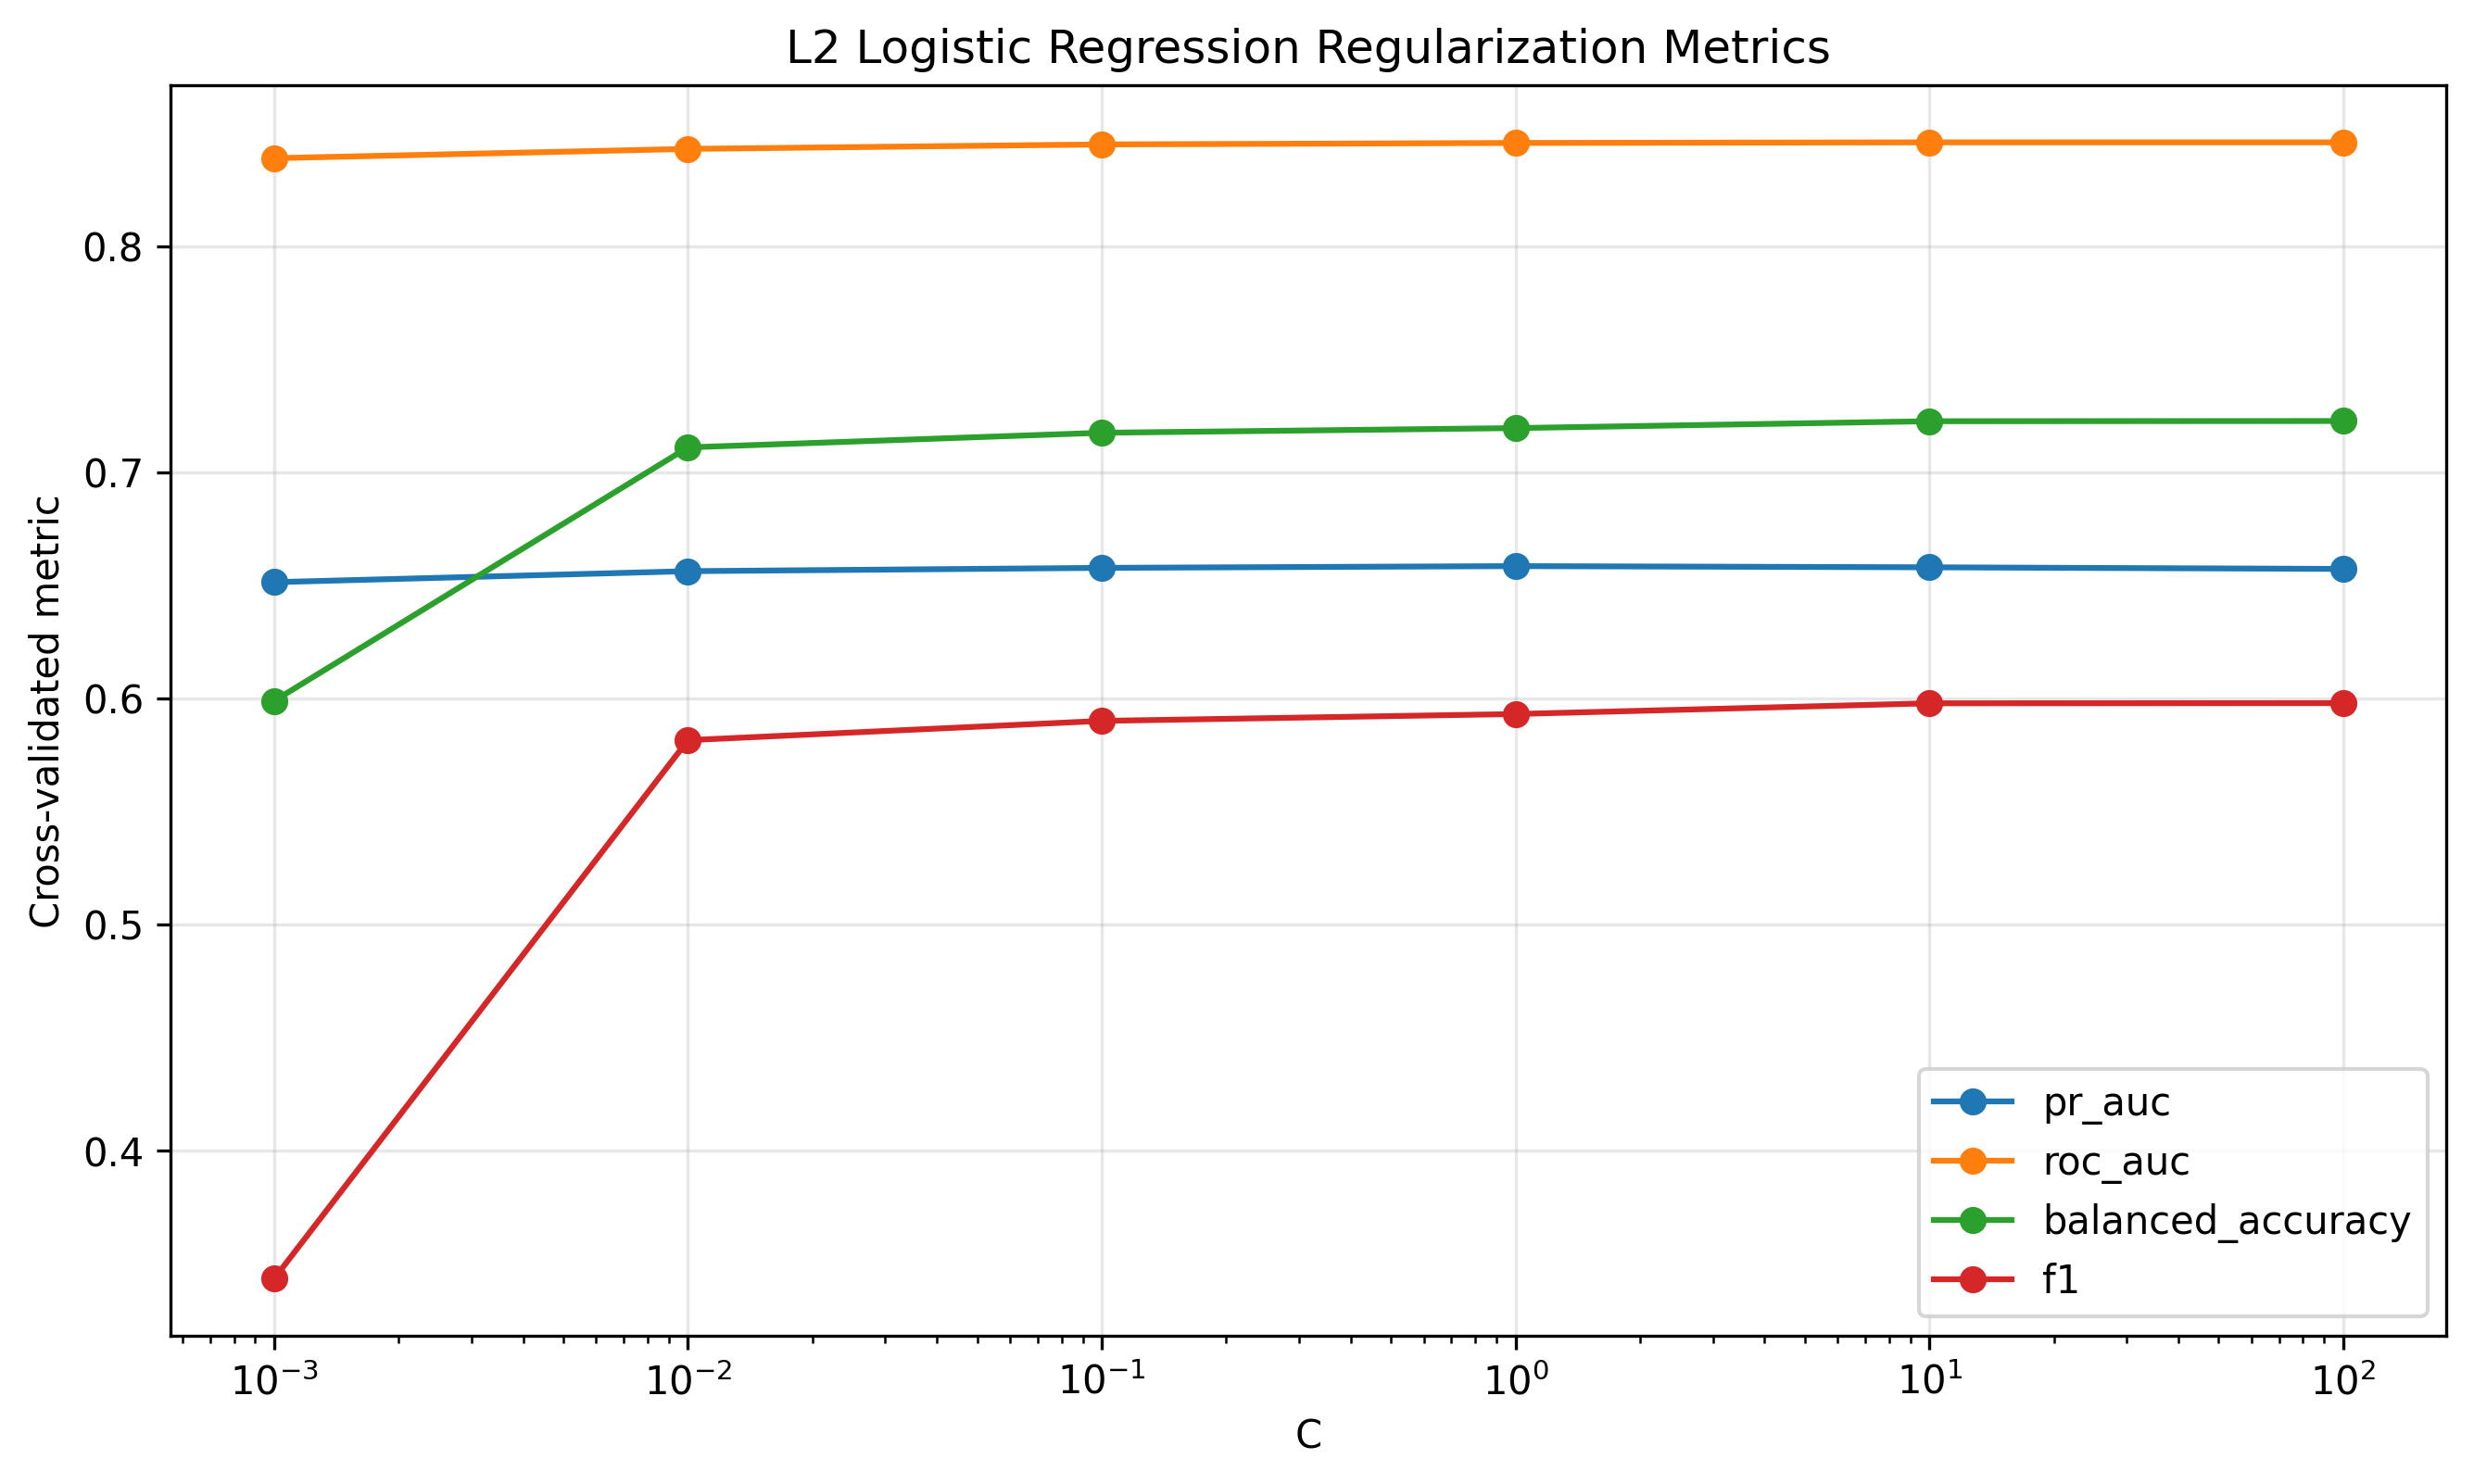
\includegraphics[width=0.82\textwidth]{../figures/logistic_l2_regularization_metrics.png}
\caption{L2 logistic regression metrics over the regularization grid.}
\label{fig:l2-regularization}
\end{figure}

The L1 grid in Table~\ref{tab:l1-regularization} and Figure~\ref{fig:l1-regularization} shows a more visible effect of very strong regularization. At \(C=0.001\), the L1 model effectively predicts no churners, so recall and F1 are zero and PR-AUC equals the positive-class prevalence. Once \(C\) reaches \(0.1\) or larger, the L1 model behaves similarly to L2 logistic regression. This suggests that mild L1 regularization is compatible with the predictive structure in the data, but excessive sparsity removes too much useful signal.

Here again, the exact best value should not be overinterpreted. \(C=1\) and \(C=10\) differ only slightly. The important conclusion is that the L1 model needs enough flexibility to keep the relevant one-hot and numeric signals active.

\begin{table}[H]
\centering
\small
\begin{tabular}{rrrrrrrr}
\toprule
\(C\) & Acc. & Bal. acc. & Prec. & Recall & F1 & ROC-AUC & PR-AUC \\
\midrule
0.001 & 0.735 & 0.500 & 0.000 & 0.000 & 0.000 & 0.500 & 0.265 \\
0.01 & 0.794 & 0.673 & 0.684 & 0.416 & 0.517 & 0.825 & 0.632 \\
0.1 & 0.801 & 0.714 & 0.655 & 0.528 & 0.585 & 0.844 & 0.658 \\
1 & 0.802 & 0.720 & 0.654 & 0.543 & 0.593 & 0.846 & 0.659 \\
10 & 0.803 & 0.722 & 0.654 & 0.548 & 0.597 & 0.846 & 0.658 \\
\bottomrule
\end{tabular}
\caption{L1 logistic regression regularization grid.}
\label{tab:l1-regularization}
\end{table}

\begin{figure}[H]
\centering
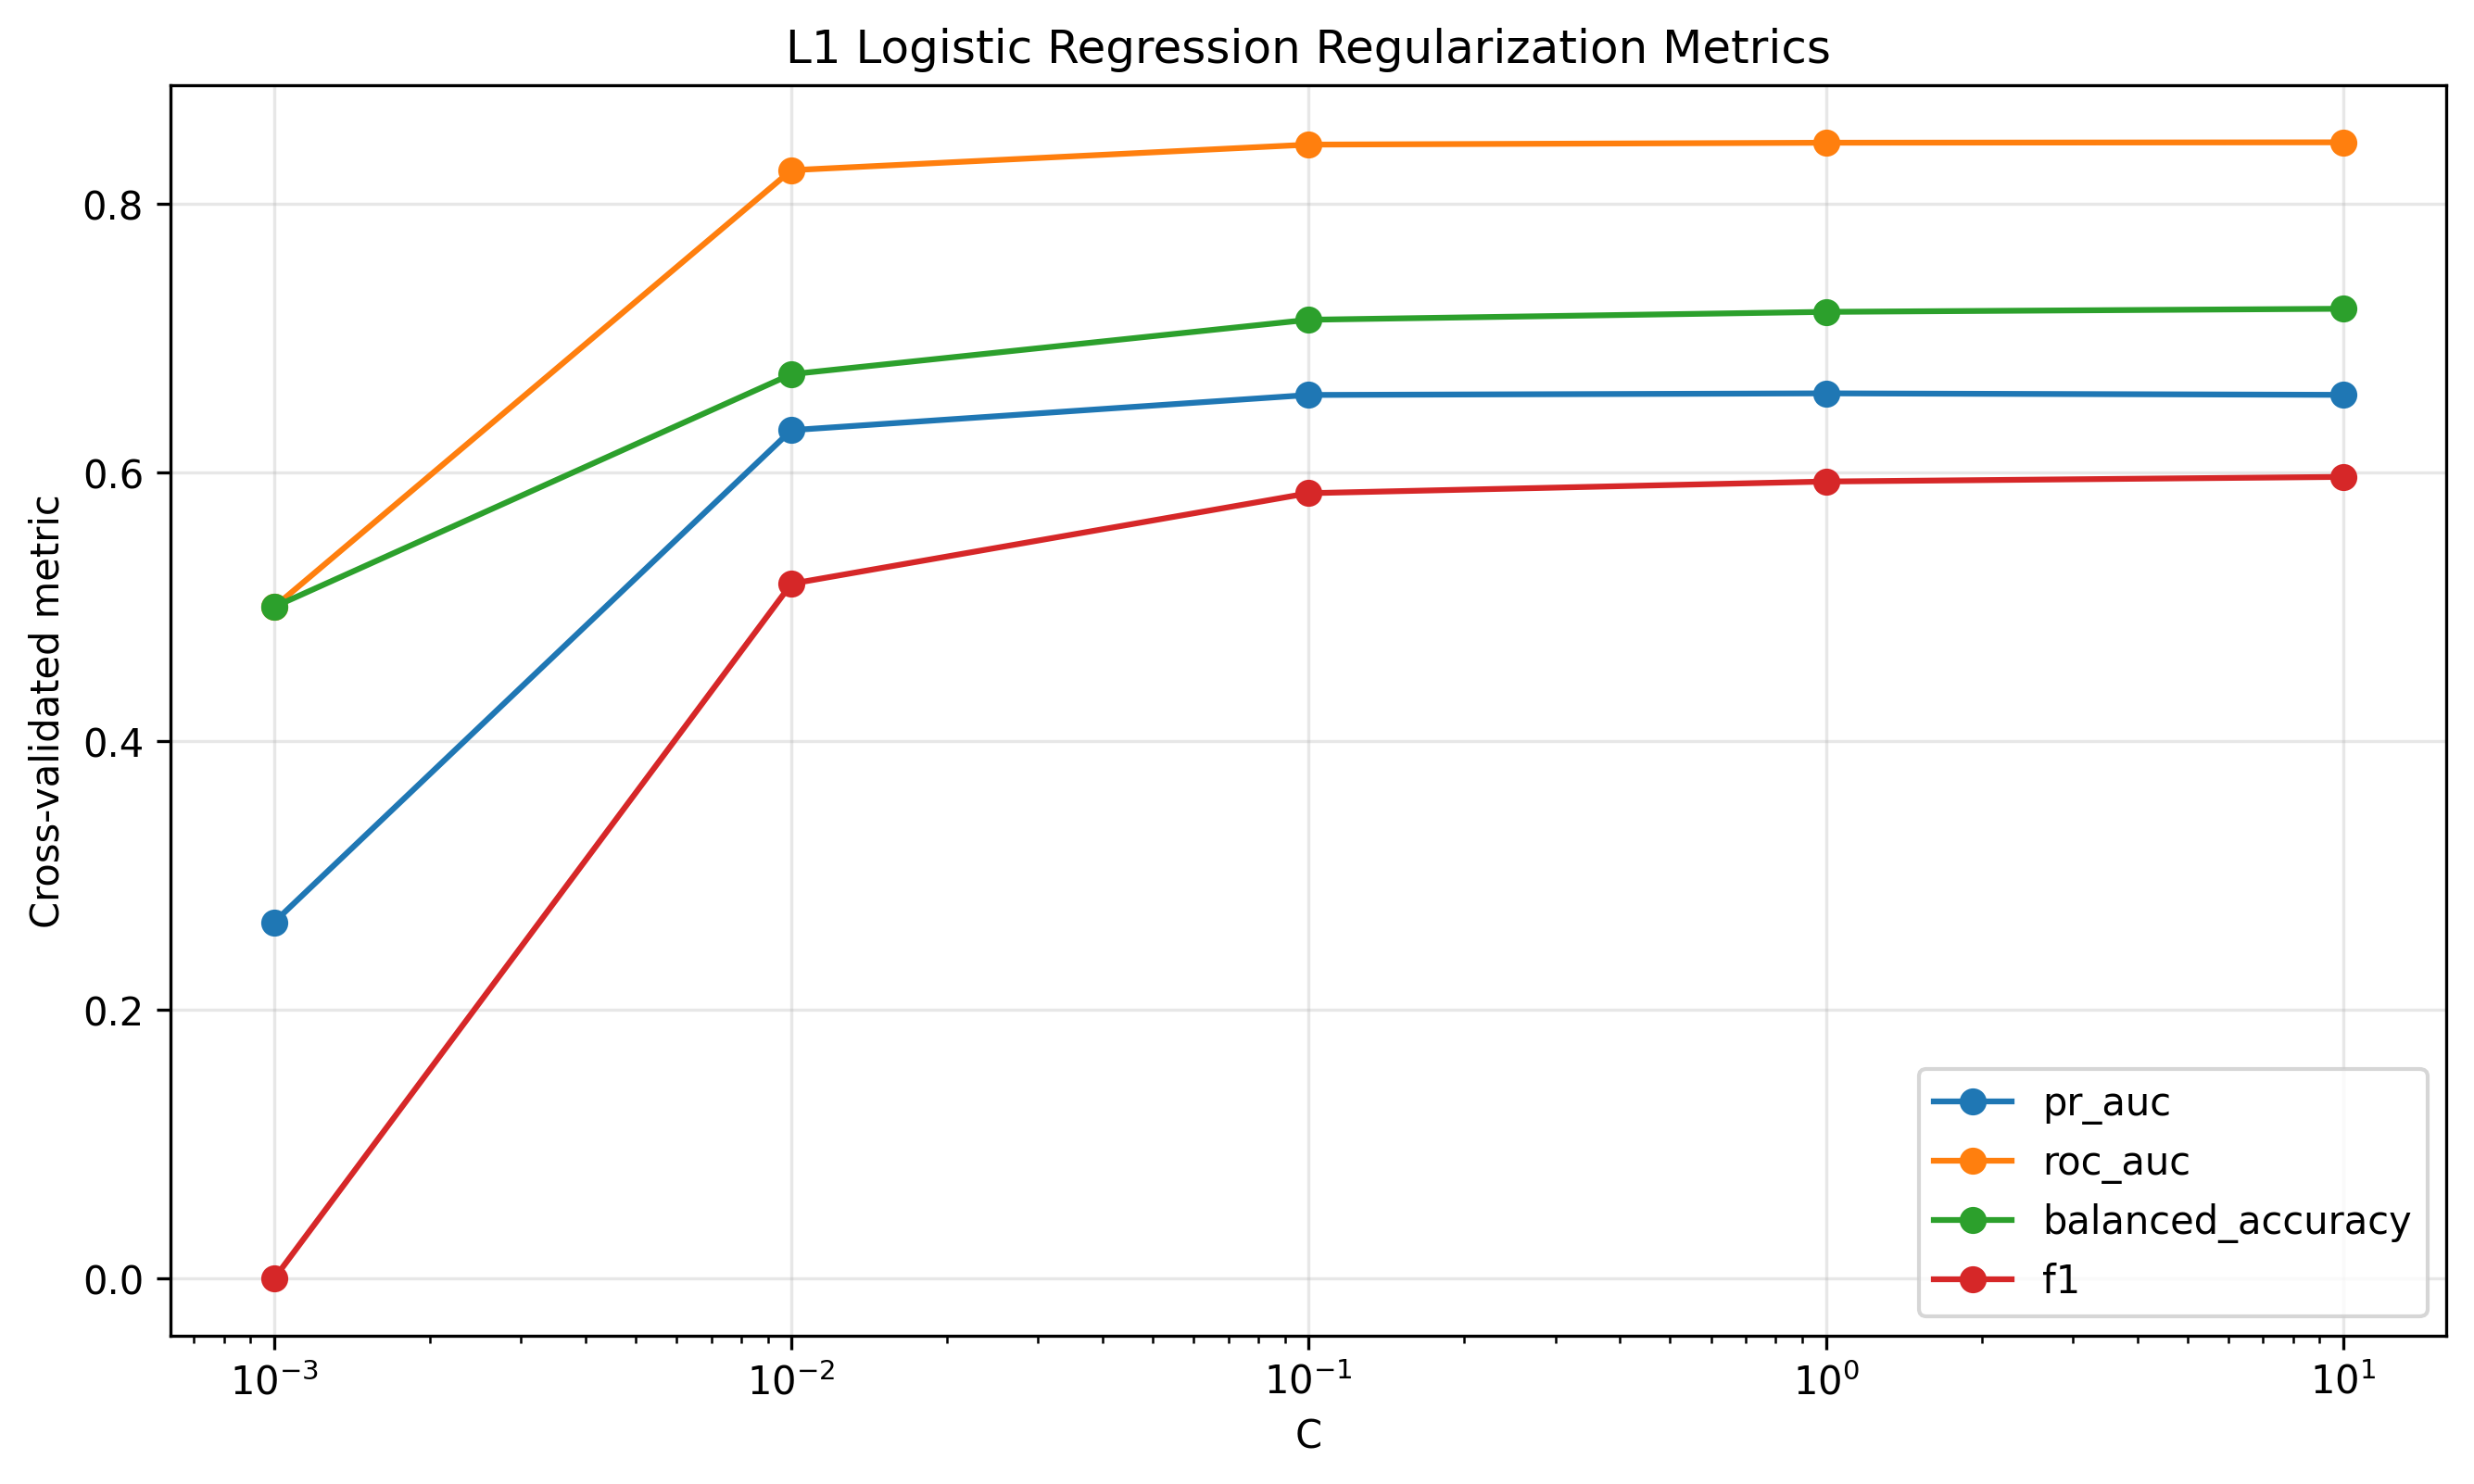
\includegraphics[width=0.82\textwidth]{../figures/logistic_l1_regularization_metrics.png}
\caption{L1 logistic regression metrics over the regularization grid.}
\label{fig:l1-regularization}
\end{figure}

\subsection{Selected logistic model and coefficient interpretation}

For interpretation, the selected model is the L2 logistic regression model with \(C=1\). This is not selected because it is statistically proven to be uniquely optimal. Rather, it is a representative, stable, standard logistic model from the high-performing regularization region. It has development-stage PR-AUC essentially equal to the best L2 configurations, and it supports straightforward coefficient interpretation. The model is fitted on the full training set only for coefficient extraction. These fitted coefficients are not used to report in-sample performance.

Table~\ref{tab:logistic-coefficients} and Figure~\ref{fig:logistic-coefficients} show the largest coefficients by absolute value. The strongest negative coefficient is \texttt{tenure}, meaning longer-tenure customers receive lower fitted churn scores. \texttt{Contract\_Two year} also has a negative coefficient, consistent with the EDA finding that two-year contracts have low churn rates. The strongest positive coefficients are \texttt{InternetService\_Fiber optic}, \texttt{Contract\_Month-to-month}, and \texttt{TotalCharges}, all associated with higher fitted churn scores in this linear model.

A notable pattern is that \texttt{MonthlyCharges} has a negative coefficient while \texttt{TotalCharges} has a positive coefficient. This should not be interpreted in isolation as a simple marginal effect. Logistic regression estimates partial associations after controlling for the other encoded features. Since \texttt{tenure}, \texttt{MonthlyCharges}, and \texttt{TotalCharges} are related, their coefficients reflect a conditional linear decomposition rather than the marginal patterns seen in EDA.

\begin{table}[H]
\centering
\small
\begin{tabular}{lrrl}
\toprule
Feature & Coef. & Odds ratio & Direction \\
\midrule
\texttt{tenure} & -1.255 & 0.285 & lower churn score \\
\texttt{Contract\_Two year} & -0.759 & 0.468 & lower churn score \\
\texttt{InternetService\_Fiber optic} & 0.648 & 1.912 & higher churn score \\
\texttt{InternetService\_DSL} & -0.644 & 0.525 & lower churn score \\
\texttt{MonthlyCharges} & -0.601 & 0.548 & lower churn score \\
\texttt{Contract\_Month-to-month} & 0.586 & 1.797 & higher churn score \\
\texttt{TotalCharges} & 0.533 & 1.703 & higher churn score \\
\texttt{PaperlessBilling\_No} & -0.331 & 0.718 & lower churn score \\
\texttt{DeviceProtection\_No internet service} & -0.293 & 0.746 & lower churn score \\
\texttt{OnlineBackup\_No internet service} & -0.293 & 0.746 & lower churn score \\
\texttt{OnlineSecurity\_No internet service} & -0.293 & 0.746 & lower churn score \\
\texttt{InternetService\_No} & -0.293 & 0.746 & lower churn score \\
\bottomrule
\end{tabular}
\caption{Largest selected logistic regression coefficients by absolute value.}
\label{tab:logistic-coefficients}
\end{table}

\begin{figure}[H]
\centering
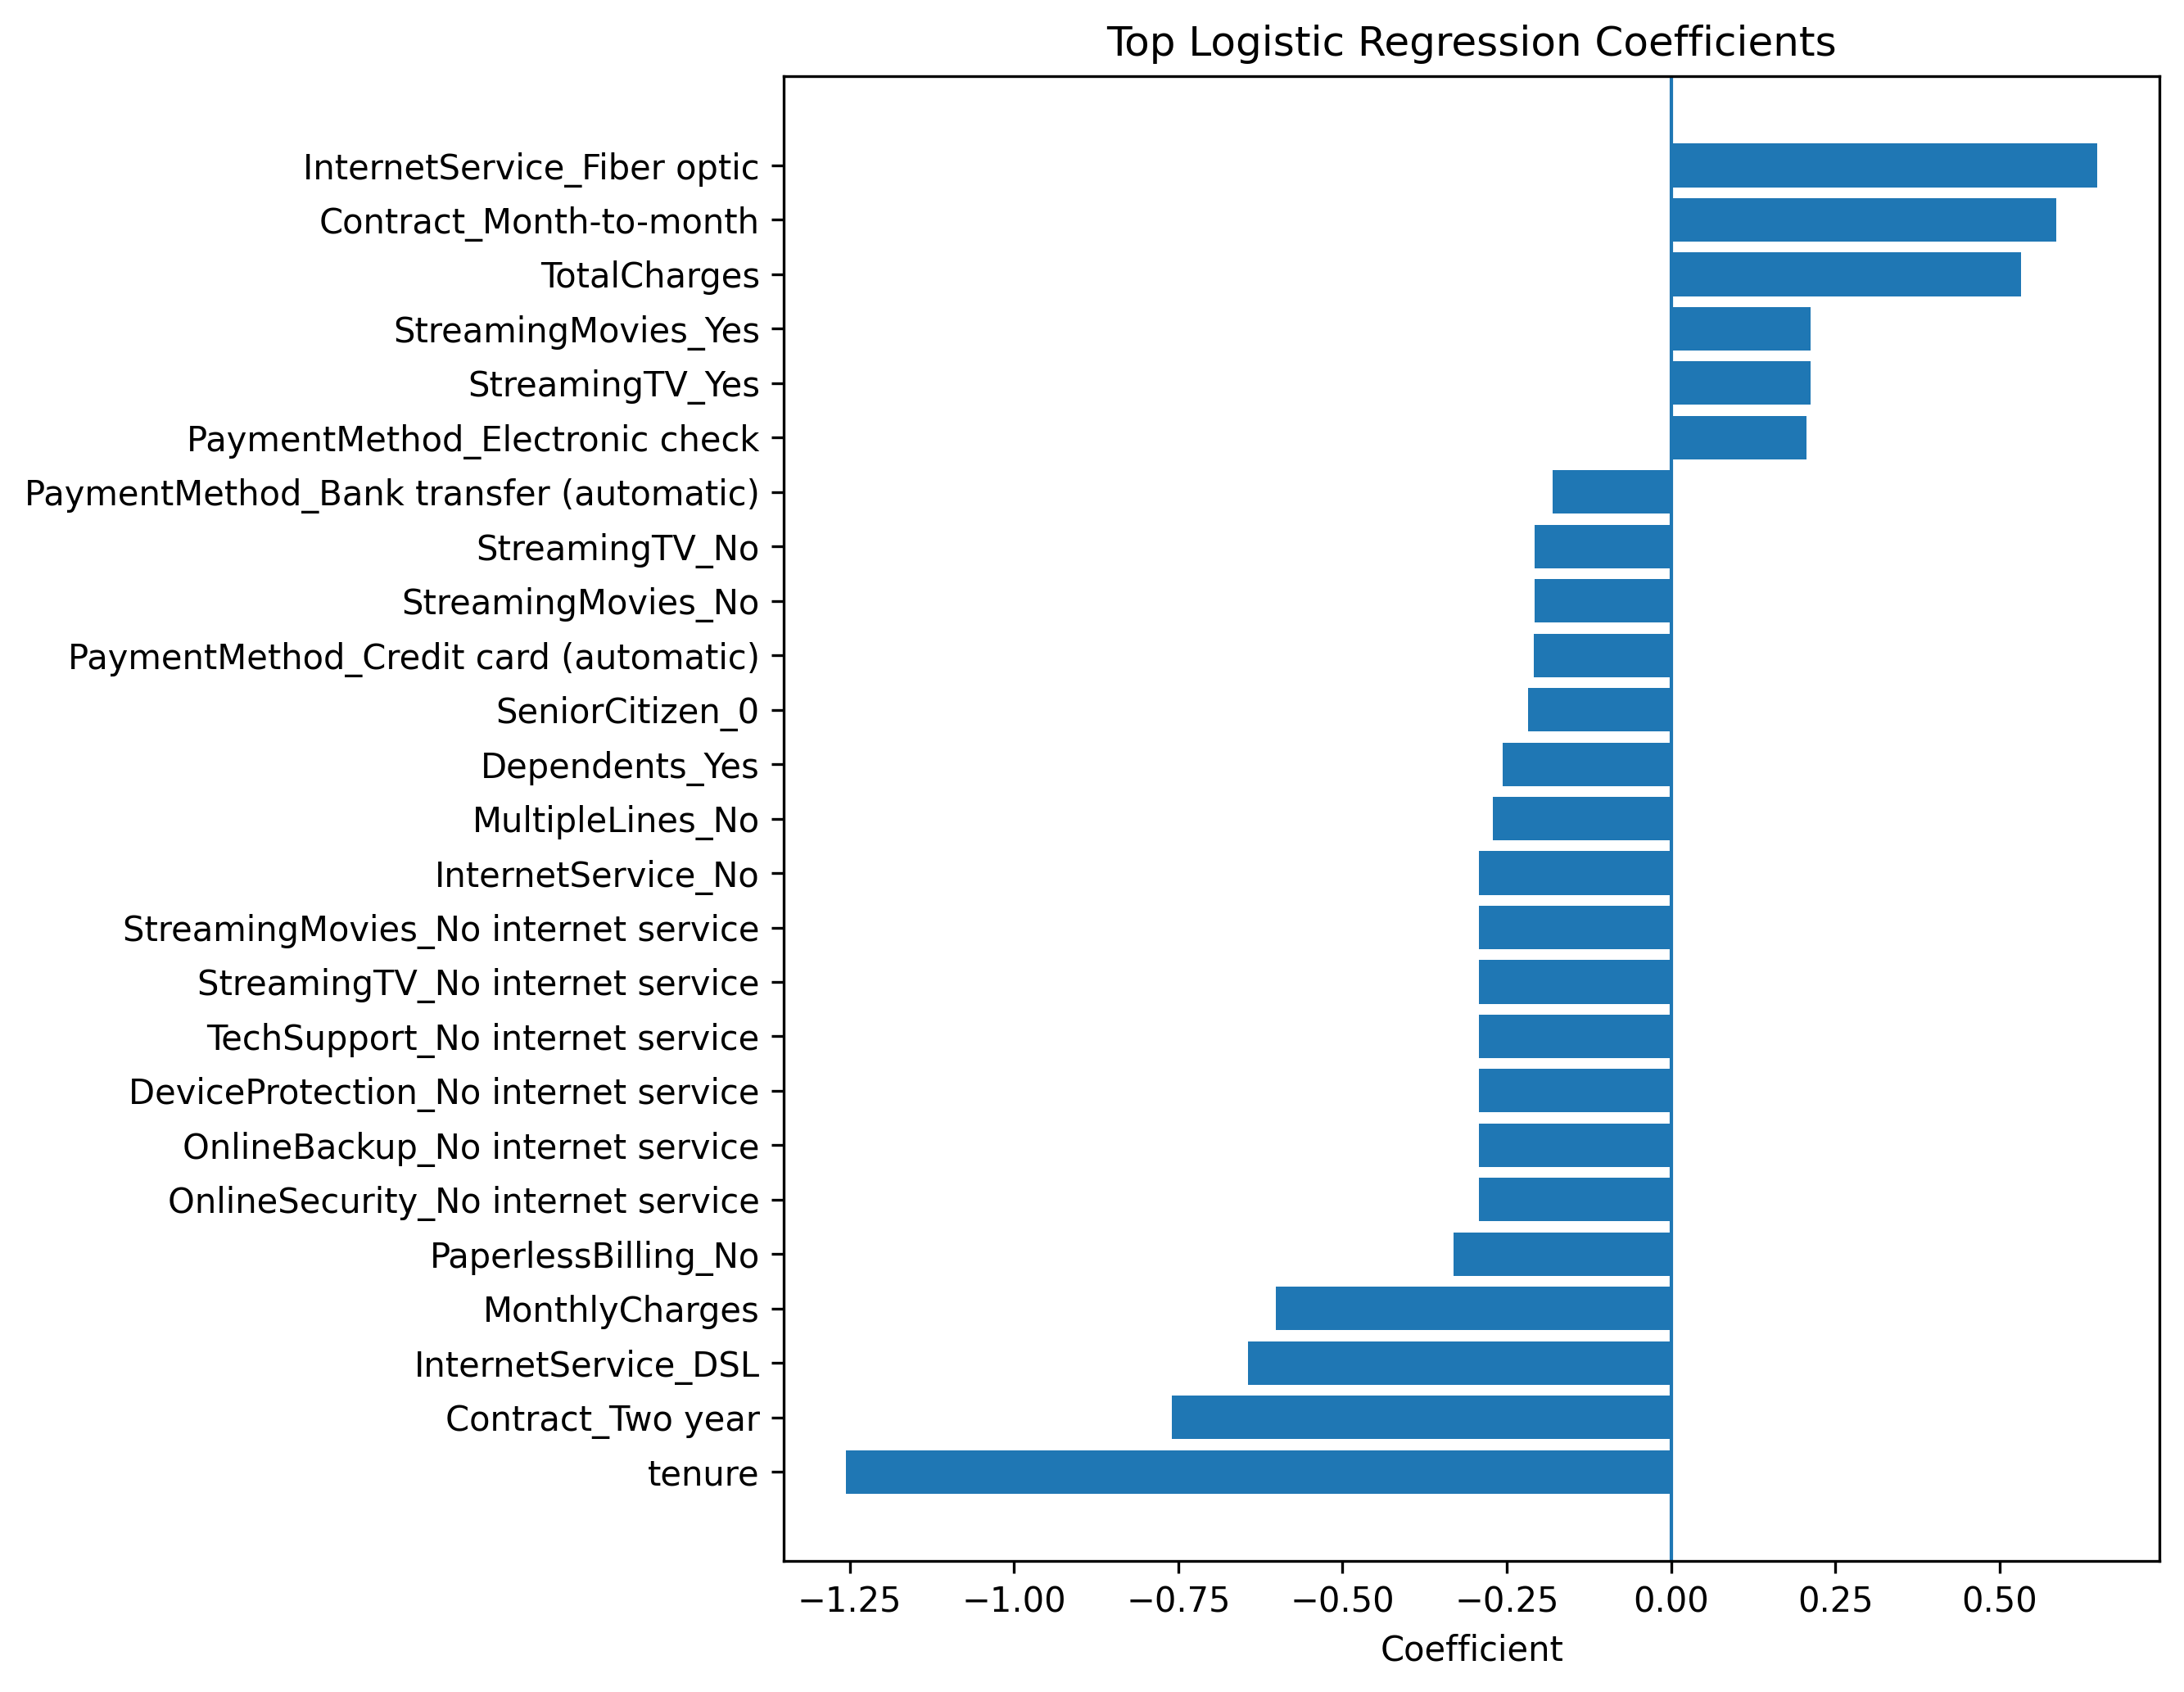
\includegraphics[width=0.82\textwidth]{../figures/logistic_top_coefficients.png}
\caption{Top logistic regression coefficients by absolute magnitude.}
\label{fig:logistic-coefficients}
\end{figure}

\subsection{Threshold tradeoff}

The default logistic regression threshold is \(0.5\), but threshold choice controls the tradeoff between recall, precision, and specificity. Table~\ref{tab:threshold-tradeoff} reports selected thresholds using out-of-fold predicted probabilities. Lowering the threshold increases recall and the predicted positive rate, while raising the threshold increases precision and specificity.

At threshold \(0.50\), the selected L2 logistic model has precision \(0.652\), recall \(0.544\), specificity \(0.895\), and F1 \(0.593\). At threshold \(0.30\), recall increases to \(0.767\), while precision decreases to \(0.541\) and specificity decreases to \(0.765\). The F1 score is highest around thresholds \(0.30\) to \(0.35\) among the displayed values. This does not mean that the final threshold should be chosen here. Final threshold selection should be postponed until model families are compared and the project objective is specified more explicitly.

\begin{table}[H]
\centering
\small
\begin{tabular}{rrrrrrrr}
\toprule
Threshold & Acc. & Bal. acc. & Prec. & Recall & Spec. & F1 & Pred. pos. rate \\
\midrule
0.10 & 0.611 & 0.716 & 0.401 & 0.942 & 0.491 & 0.562 & 0.624 \\
0.20 & 0.711 & 0.757 & 0.475 & 0.854 & 0.659 & 0.610 & 0.477 \\
0.25 & 0.742 & 0.766 & 0.509 & 0.817 & 0.715 & 0.627 & 0.426 \\
0.30 & 0.766 & 0.766 & 0.541 & 0.767 & 0.765 & 0.634 & 0.376 \\
0.35 & 0.782 & 0.761 & 0.571 & 0.717 & 0.805 & 0.635 & 0.334 \\
0.40 & 0.790 & 0.750 & 0.594 & 0.664 & 0.836 & 0.627 & 0.297 \\
0.50 & 0.802 & 0.719 & 0.652 & 0.544 & 0.895 & 0.593 & 0.221 \\
0.60 & 0.797 & 0.669 & 0.710 & 0.397 & 0.942 & 0.509 & 0.148 \\
0.70 & 0.775 & 0.594 & 0.779 & 0.210 & 0.978 & 0.331 & 0.072 \\
\bottomrule
\end{tabular}
\caption{Threshold tradeoff for selected L2 logistic regression using out-of-fold probabilities.}
\label{tab:threshold-tradeoff}
\end{table}

\begin{figure}[H]
\centering
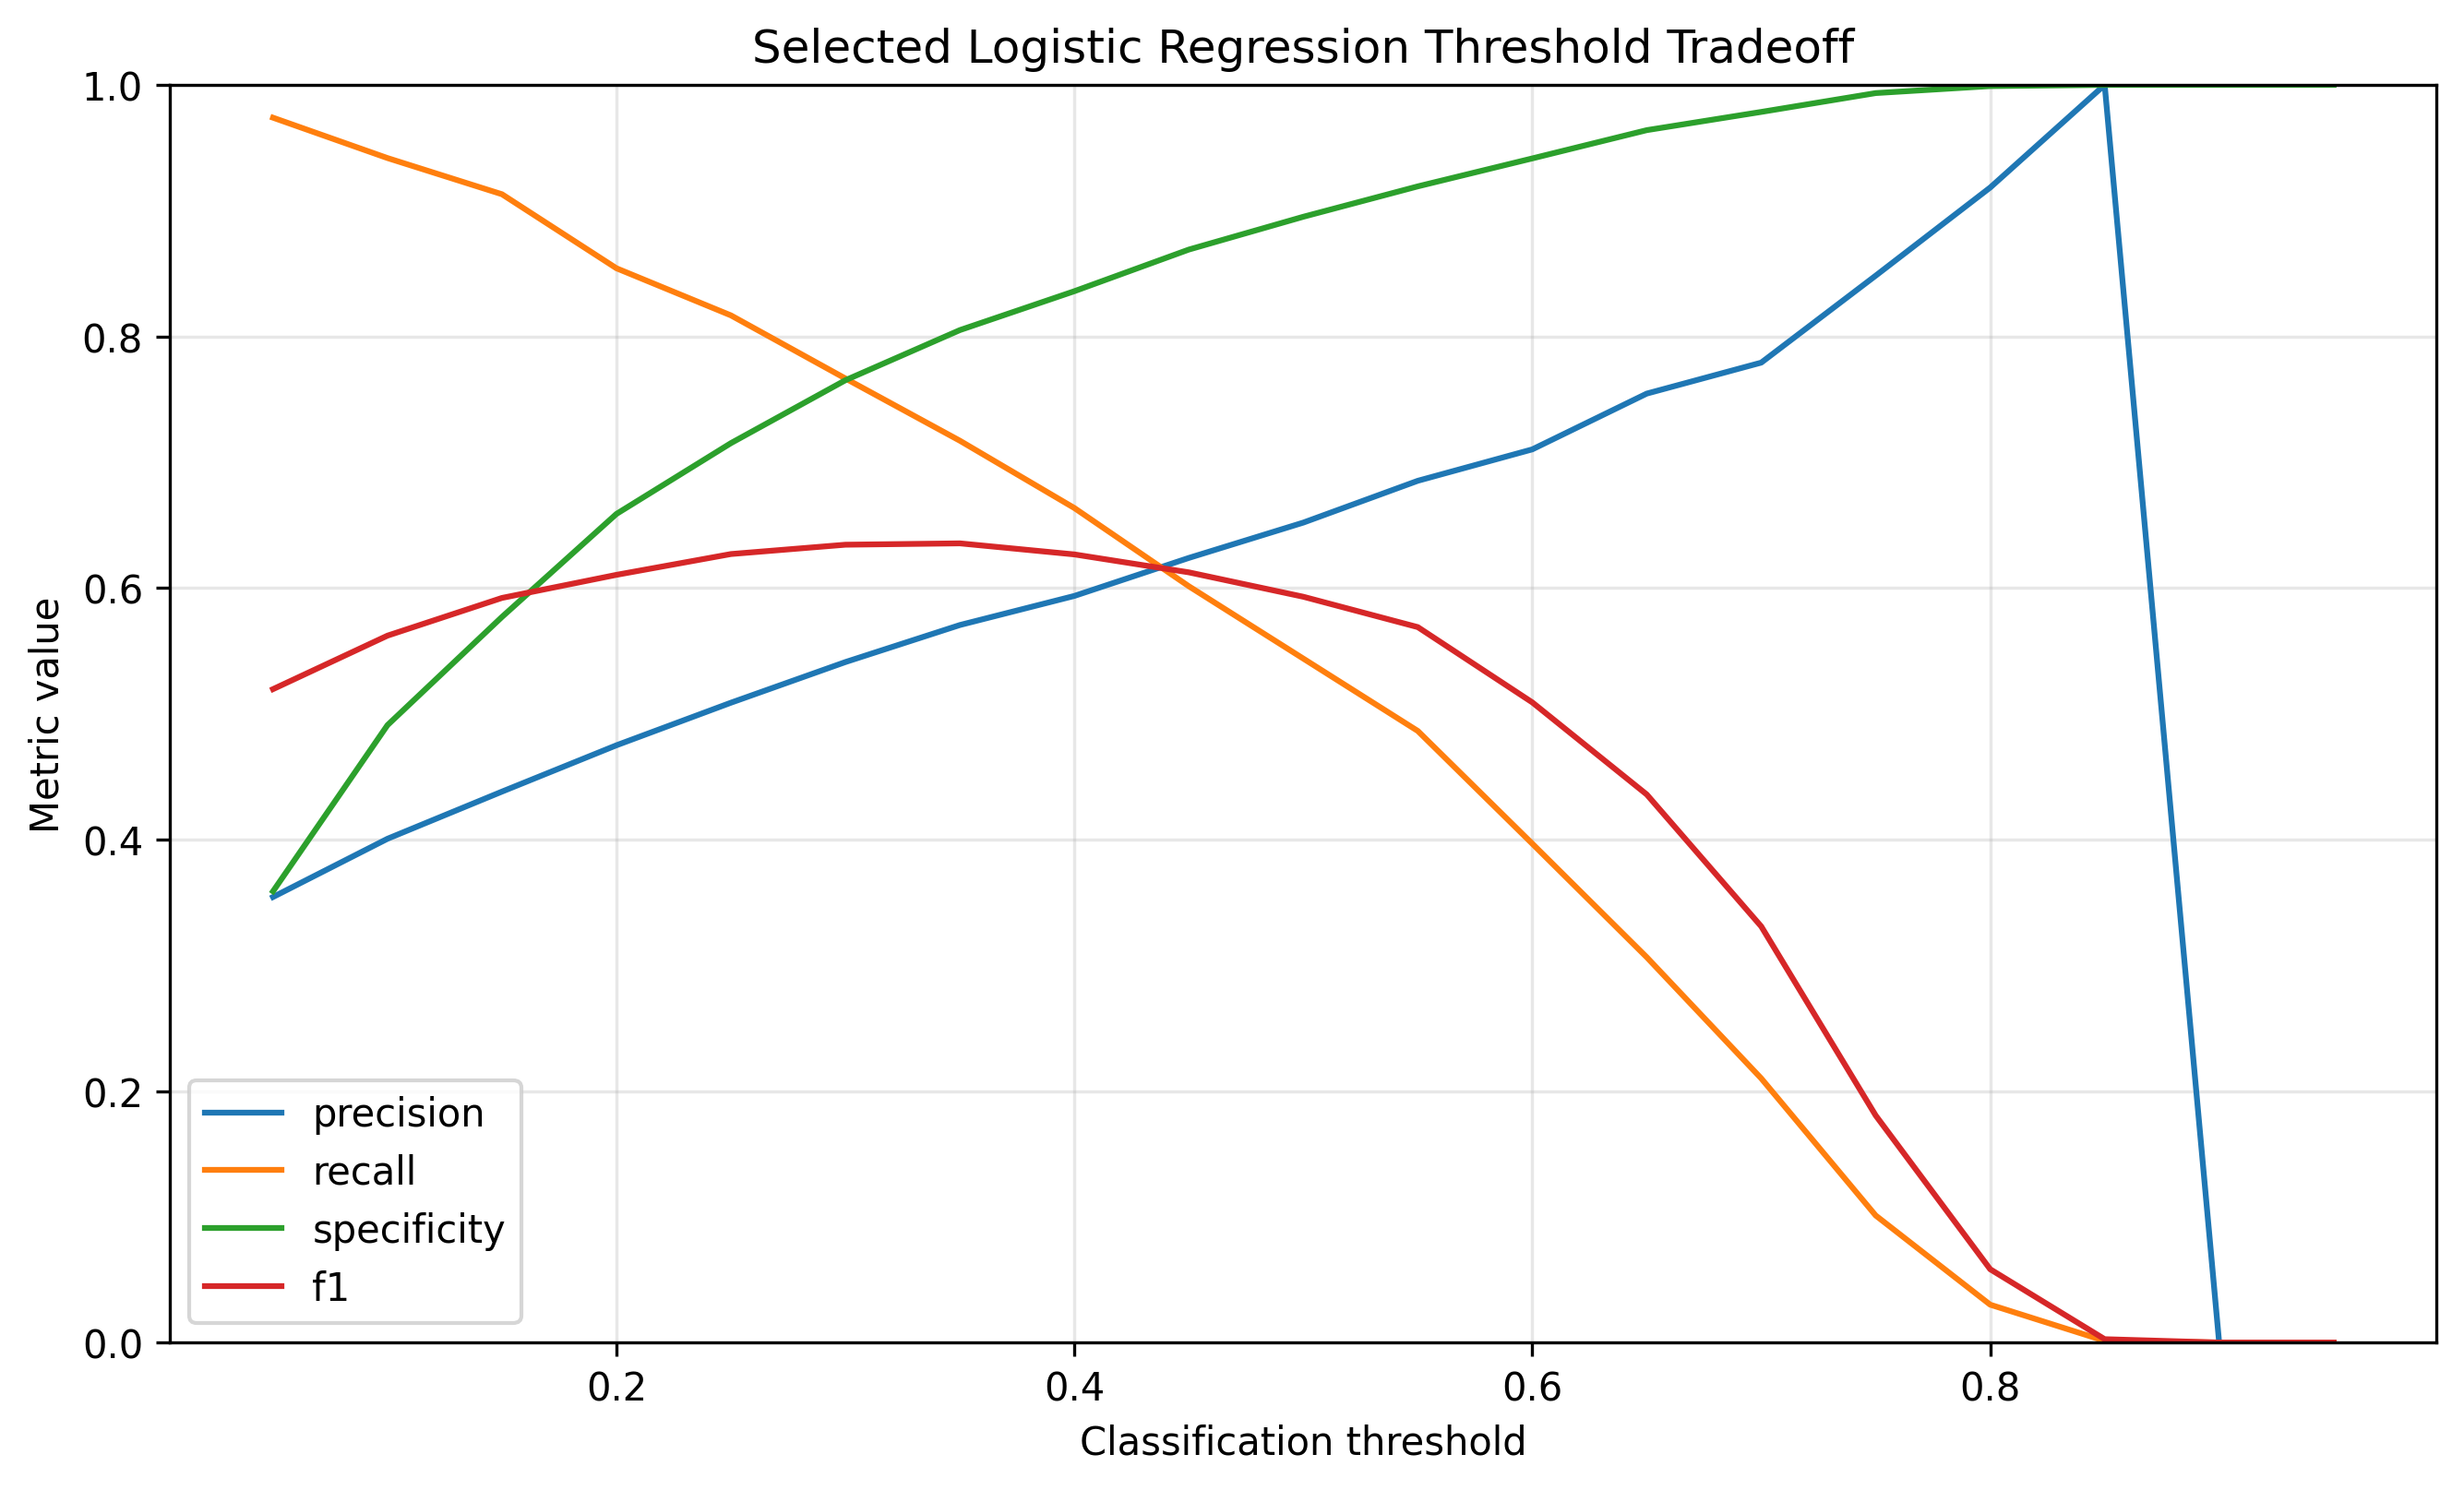
\includegraphics[width=0.82\textwidth]{../figures/logistic_threshold_tradeoff.png}
\caption{Threshold tradeoff for selected L2 logistic regression.}
\label{fig:threshold-tradeoff}
\end{figure}

\subsection{ROC and precision-recall curves}

Figures~\ref{fig:logistic-roc} and~\ref{fig:logistic-pr} summarize threshold-independent ranking performance for the selected logistic regression model. The ROC curve has AUC approximately \(0.846\), indicating that the model ranks churners above non-churners substantially better than a random ranking. The precision-recall curve has AUC approximately \(0.658\), compared with a positive-rate baseline of approximately \(0.265\). This is important because churn is the minority class, and PR-AUC focuses directly on the quality of positive churn retrieval.

\begin{figure}[H]
\centering
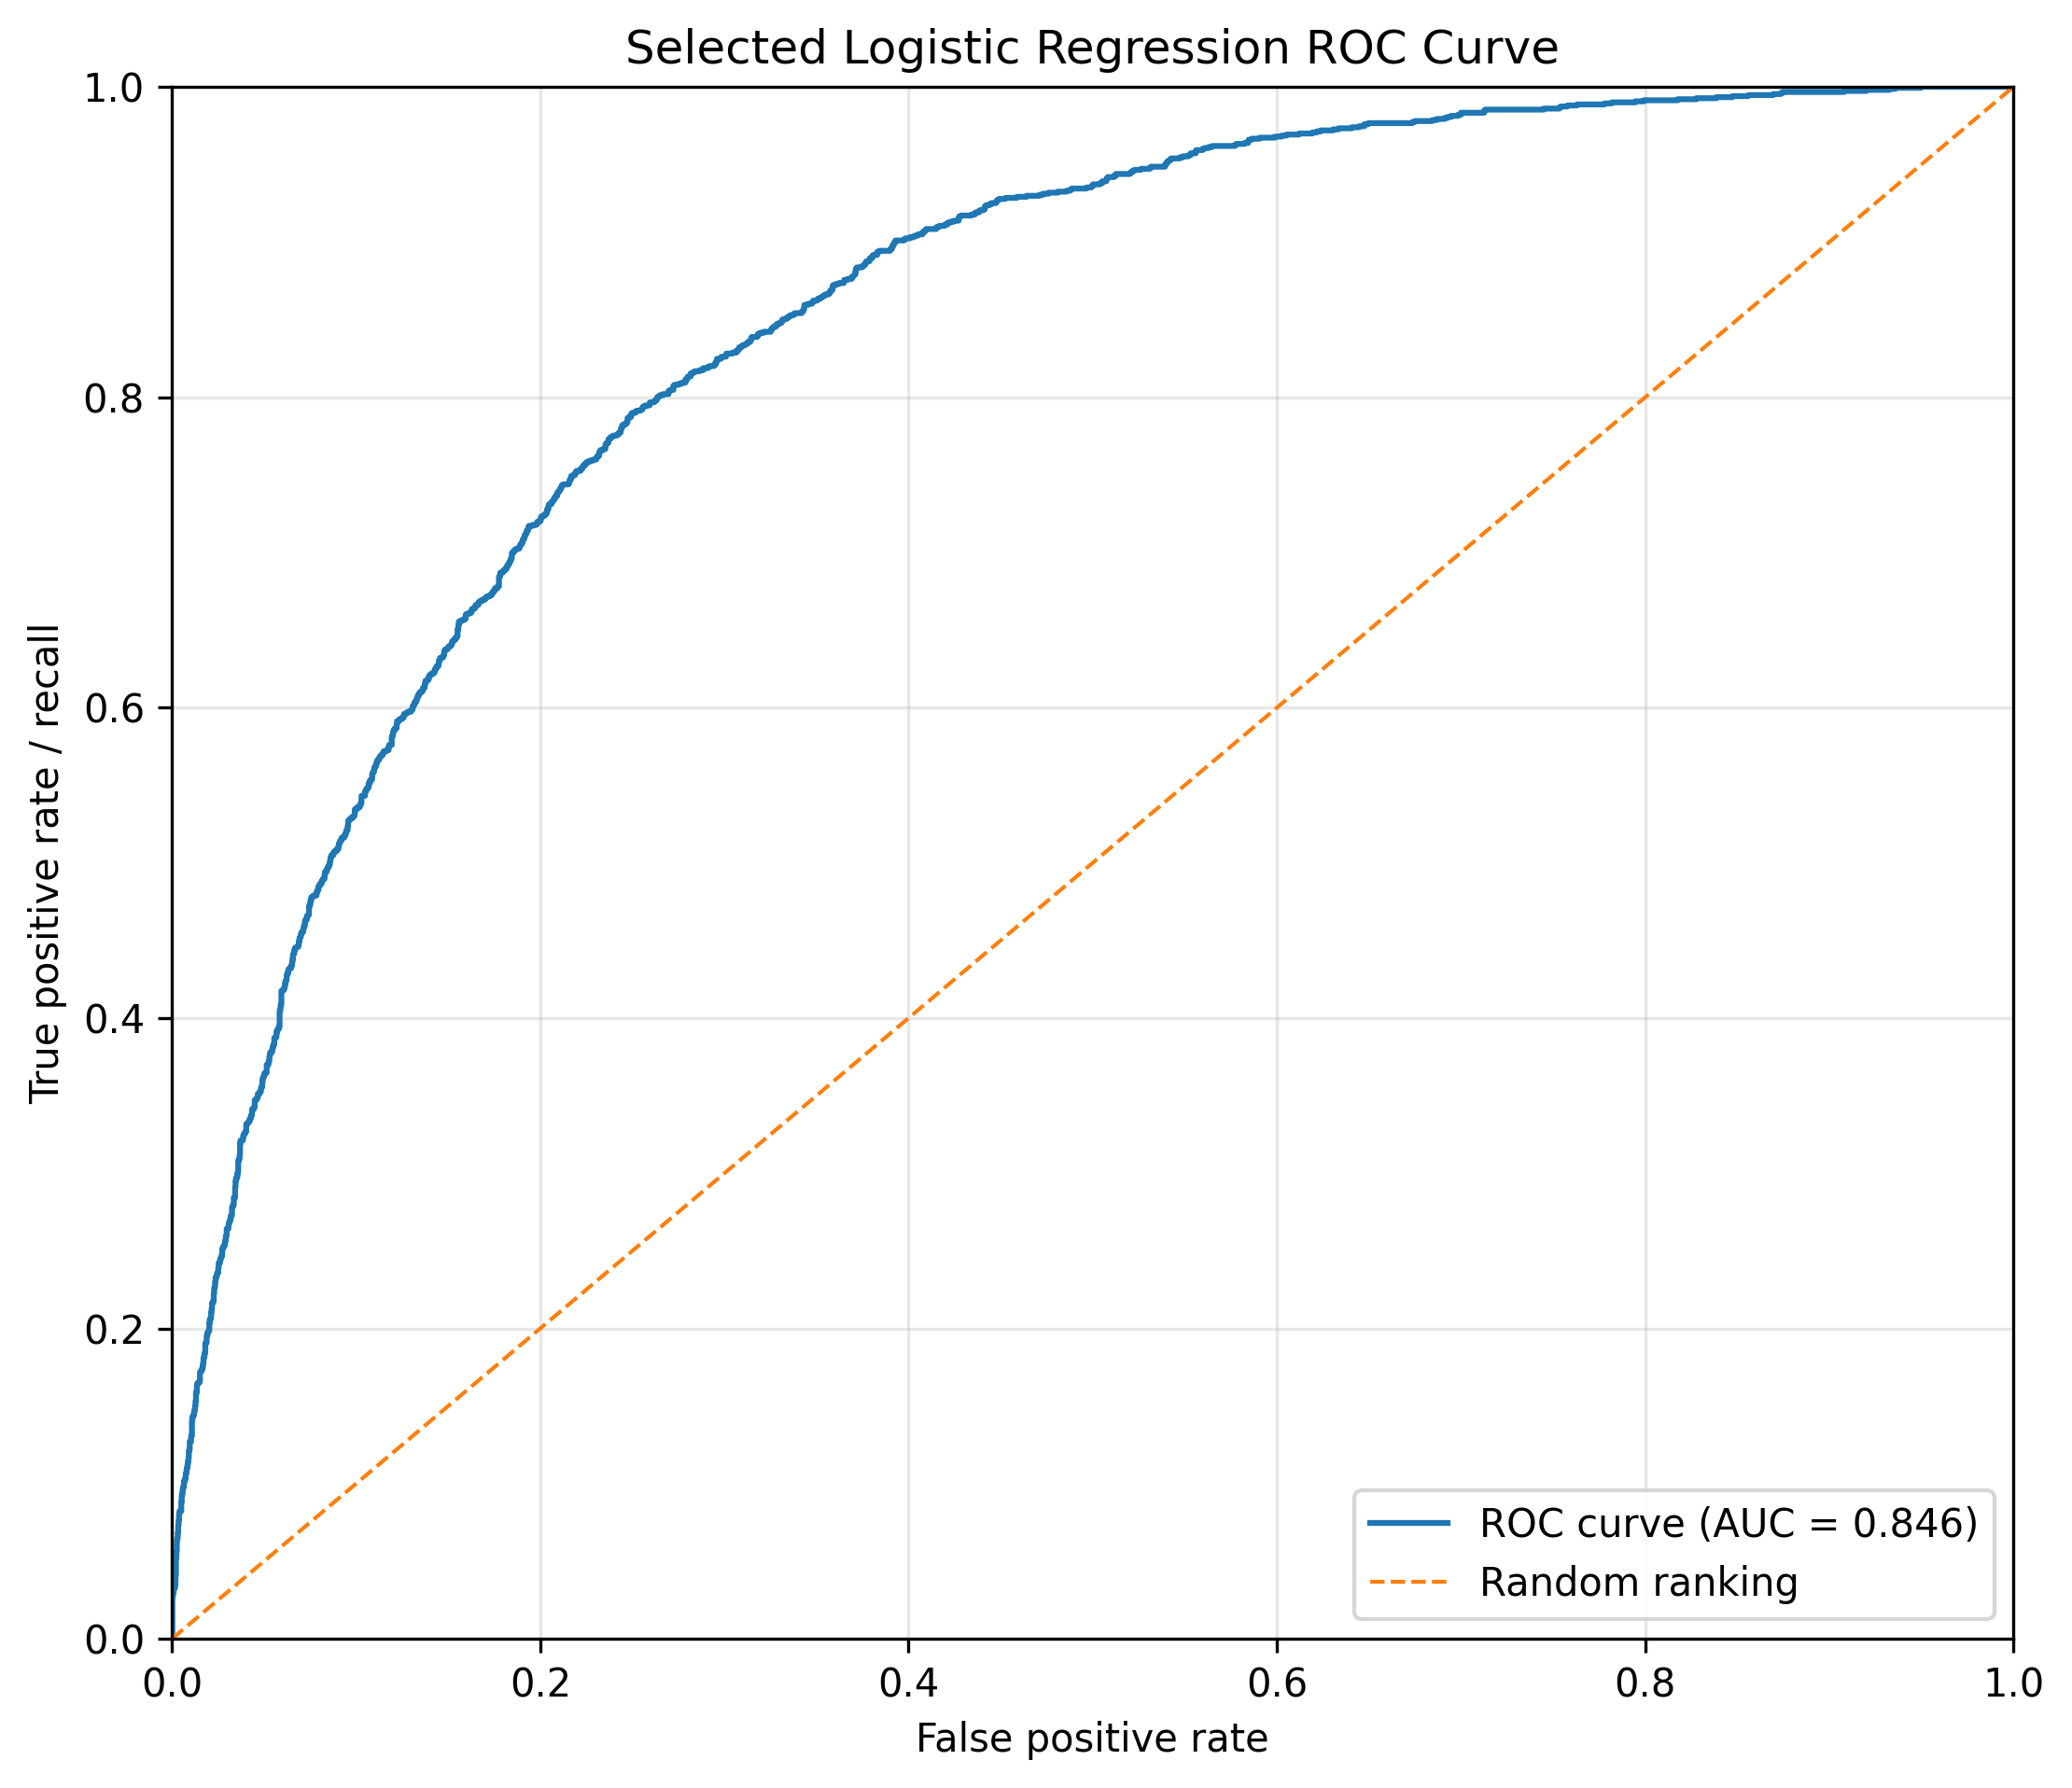
\includegraphics[width=0.76\textwidth]{../figures/logistic_roc_curve.png}
\caption{ROC curve for selected L2 logistic regression.}
\label{fig:logistic-roc}
\end{figure}

\begin{figure}[H]
\centering
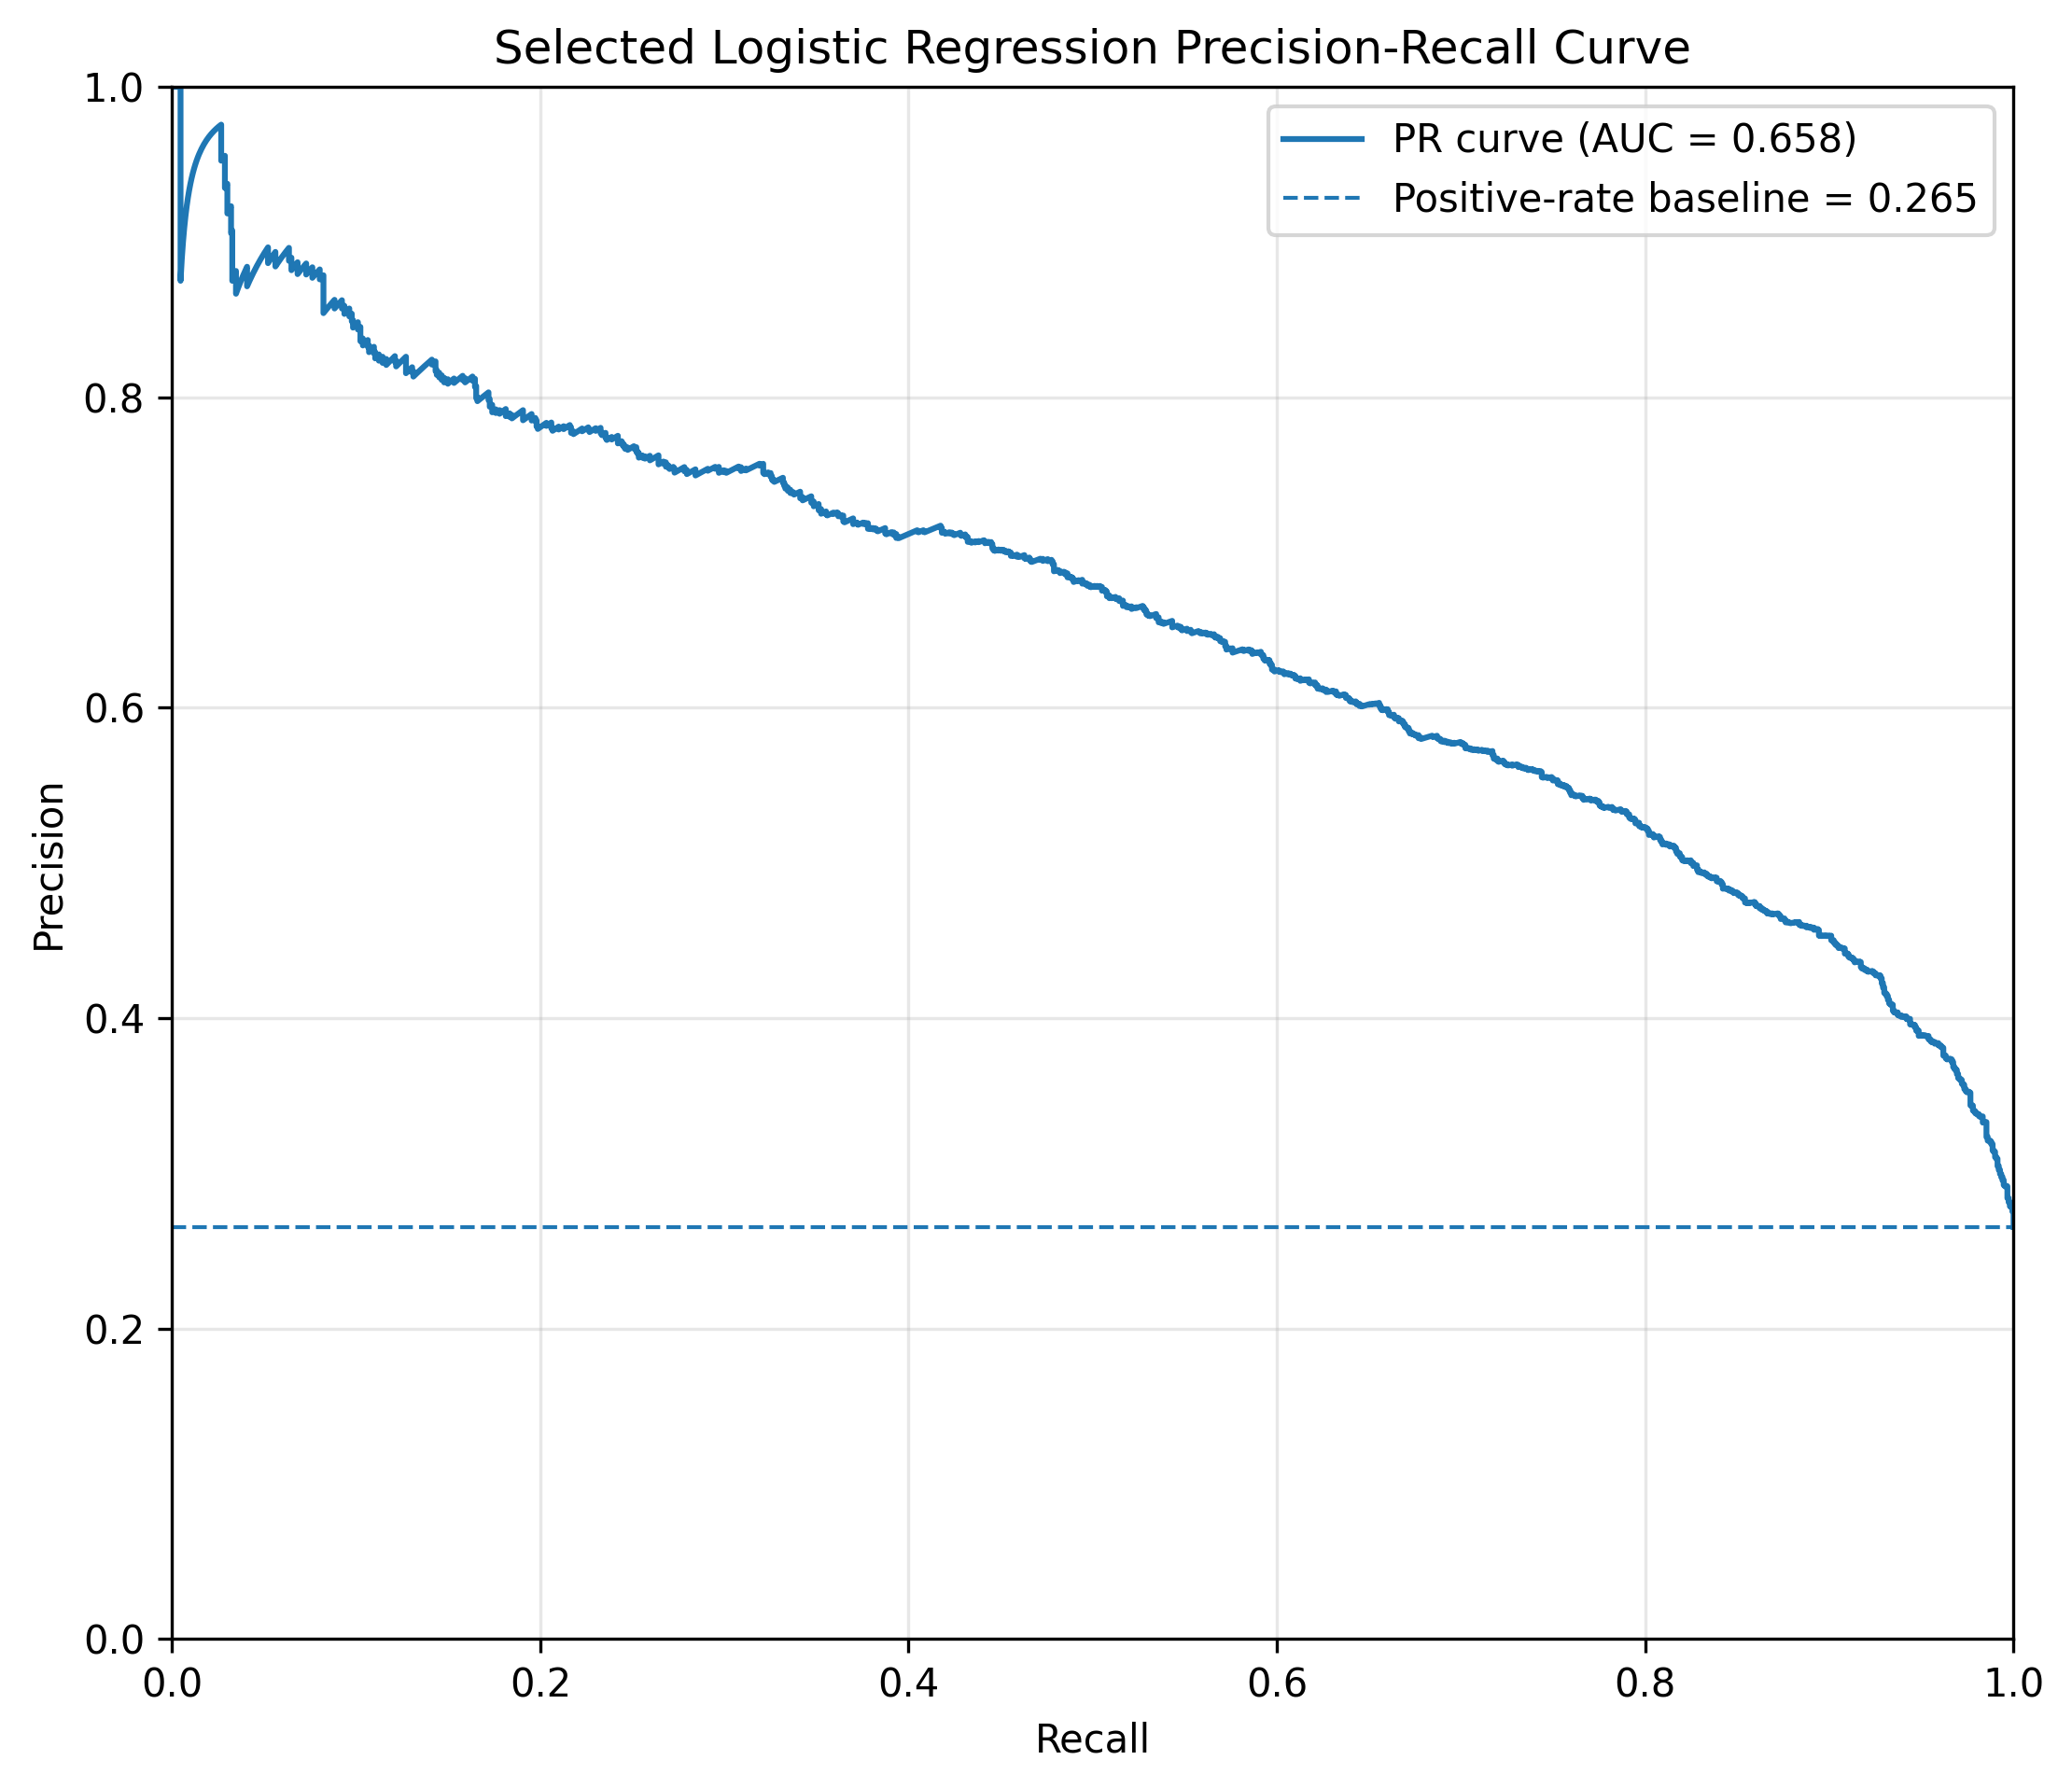
\includegraphics[width=0.76\textwidth]{../figures/logistic_precision_recall_curve.png}
\caption{Precision-recall curve for selected L2 logistic regression.}
\label{fig:logistic-pr}
\end{figure}

\subsection{Summary}

Logistic regression is a strong first learned model for the churn task. It clearly improves on non-informative baselines and provides useful probability rankings, with ROC-AUC around \(0.846\) and PR-AUC around \(0.658\). L1 and L2 regularization give very similar cross-validated performance once regularization is not excessively strong. Ridge classification is slightly weaker but remains a reasonable least-squares linear baseline.

The regularization grids show that the exact value of \(C\) is not the main conclusion. The important development-stage lesson is that extremely strong regularization underfits, while a broad moderate-to-weak regularization region performs similarly. This is why the selected L2 logistic model should be understood as a representative stable linear benchmark rather than a uniquely optimal hyperparameter setting.

The class-weighted logistic regression variant demonstrates the central classification tradeoff: it detects many more churners, but it also creates many more false positives. This confirms that model assessment cannot rely on accuracy alone. Confusion-matrix counts, recall, precision, specificity, ROC-AUC, PR-AUC, and threshold behaviour must be considered together.

The coefficient analysis is also useful. Tenure and two-year contracts are associated with lower fitted churn scores, while fiber optic internet, month-to-month contracts, and higher accumulated charges are associated with higher fitted churn scores. These patterns are consistent with the training-set EDA, but they remain predictive associations rather than causal effects.

This section establishes logistic regression as the first interpretable learned benchmark. Later model families should be compared against it by asking whether they improve ranking performance, reduce false positives at useful recall levels, or capture nonlinear feature interactions that linear models cannot represent directly. Final claims about model-family superiority are deferred to the later comparison and test-evaluation stages.


\newpage
\newpage
\section{k-Nearest Neighbours}
\label{sec:knn}

This section evaluates k-nearest neighbours as the first non-parametric and distance-based classifier in the project. Unlike logistic regression, which estimates a global vector of coefficients, k-nearest neighbours stores the training observations and classifies a new customer by comparing that customer with nearby training customers in the transformed feature space. The model is therefore useful as a contrast to the linear classifiers from Section~\ref{sec:linear-classification-and-logistic-regression}: logistic regression learns global feature weights, whereas k-nearest neighbours relies directly on local similarity.

The same validation discipline is used as in the previous modelling sections. The held-out test set is not used. All reported results are based on stratified cross-validation inside the training set. Preprocessing is kept inside the scikit-learn pipeline so that standardization and one-hot encoding are fitted only on each fold's training data.

The results in this section should be interpreted as a development-stage comparison of kNN configurations. The selected kNN model is the strongest configuration in the tried grid according to the chosen selection criterion. It is not a final statistical claim that this exact value of \(k\), distance metric, and weighting rule is uniquely optimal in the population.

\subsection{k-nearest-neighbour prediction rule}

Let the training set be
\[
\mathcal{D}_{\mathrm{train}}
=
\{(x_i,y_i)\}_{i=1}^{n},
\]
where \(x_i \in \mathbb{R}^{p}\) is the transformed feature vector for customer \(i\), and \(y_i \in \{0,1\}\) is the binary churn label. For a new customer with feature vector \(x\), k-nearest neighbours first finds the \(k\) training observations closest to \(x\) according to a chosen distance function. Let this neighbour set be denoted by
\[
\mathcal{N}_k(x).
\]
For unweighted binary classification, the estimated churn probability is the fraction of neighbours that churned:
\[
\widehat{p}(Y=1 \mid X=x)
=
\frac{1}{k}
\sum_{i \in \mathcal{N}_k(x)} y_i.
\]
The default hard classification rule at threshold \(0.5\) is
\[
\widehat{y}
=
\mathbb{1}
\left\{
\widehat{p}(Y=1 \mid X=x) \geq 0.5
\right\}.
\]
Thus, the model predicts churn when churners form at least half of the local neighbourhood.

A distance-weighted variant gives closer neighbours more influence:
\[
\widehat{p}(Y=1 \mid X=x)
=
\frac{
\sum_{i \in \mathcal{N}_k(x)} w_i(x)y_i
}{
\sum_{i \in \mathcal{N}_k(x)} w_i(x)
}.
\]
In this section, both uniform and distance-based voting are evaluated.

\subsection{Distance, scaling, and one-hot encoded features}

The distance definition is central to k-nearest neighbours. Two common distances are the Manhattan distance,
\[
d_1(x,x')
=
\sum_{j=1}^{p}
|x_j-x'_j|,
\]
and the Euclidean distance,
\[
d_2(x,x')
=
\sqrt{
\sum_{j=1}^{p}
(x_j-x'_j)^2
}.
\]
Both are special cases of the Minkowski distance. In the implementation, Manhattan distance corresponds to \(p=1\), while Euclidean distance corresponds to \(p=2\).

Because k-nearest neighbours computes distances directly from feature values, scaling is essential. Without standardization, variables with larger numeric ranges can dominate the distance calculation. For example, \texttt{TotalCharges} has a much larger raw range than \texttt{tenure} or \texttt{MonthlyCharges}. Therefore, numeric variables are standardized inside the preprocessing pipeline. Categorical variables are one-hot encoded, which allows k-nearest neighbours to operate on mixed tabular data, but also changes the geometry of the feature space. After one-hot encoding, similarity is measured in a higher-dimensional indicator space, which may not always correspond to intuitive customer similarity.

\subsection{The role of \(k\)}

The number of neighbours \(k\) controls the smoothness of the classifier. Small values of \(k\) produce highly local predictions. For example, when \(k=1\), the prediction copies the label of the single nearest training observation. This can produce low-bias but high-variance decision boundaries that are sensitive to noise.

Larger values of \(k\) average over more training observations. This usually increases bias but reduces variance, producing smoother and more stable predictions. If \(k\) becomes too large, however, predictions approach the global class distribution and the model can underfit. Therefore, \(k\) is a true model-complexity hyperparameter and must be selected using validation data rather than the held-out test set.

\subsection{Hyperparameter grid}

The k-nearest-neighbour experiment uses a transparent cross-validated grid search. The grid varies the number of neighbours, the voting scheme, and the distance metric:
\[
k \in \{1,3,5,7,11,15,21,31,51,75,101\},
\]
\[
\texttt{weights} \in \{\texttt{uniform},\texttt{distance}\},
\]
\[
p \in \{1,2\}.
\]
The \(p=1\) setting corresponds to Manhattan distance, and \(p=2\) corresponds to Euclidean distance. The selection rule chooses the configuration with the highest cross-validated PR-AUC, using balanced accuracy and F1 as secondary criteria if needed. PR-AUC is used as the primary criterion because churn is the minority class, and the positive-class ranking quality is important.

Because this grid tries multiple configurations, the winning cross-validated score should be interpreted with the model-selection caveat from Section~\ref{sec:statistical-evaluation-methodology}. It identifies a strong configuration within the tried grid, but the observed best score can contain some selection optimism.

\subsection{Grid-search behaviour}

Figure~\ref{fig:knn-pr-auc-by-k} shows the cross-validated PR-AUC across the neighbour grid. Performance improves strongly as \(k\) increases from very small values. This pattern indicates that small neighbourhoods are too noisy for this dataset. Larger neighbourhoods smooth over local irregularities and give more stable churn rankings.

\begin{figure}[H]
\centering
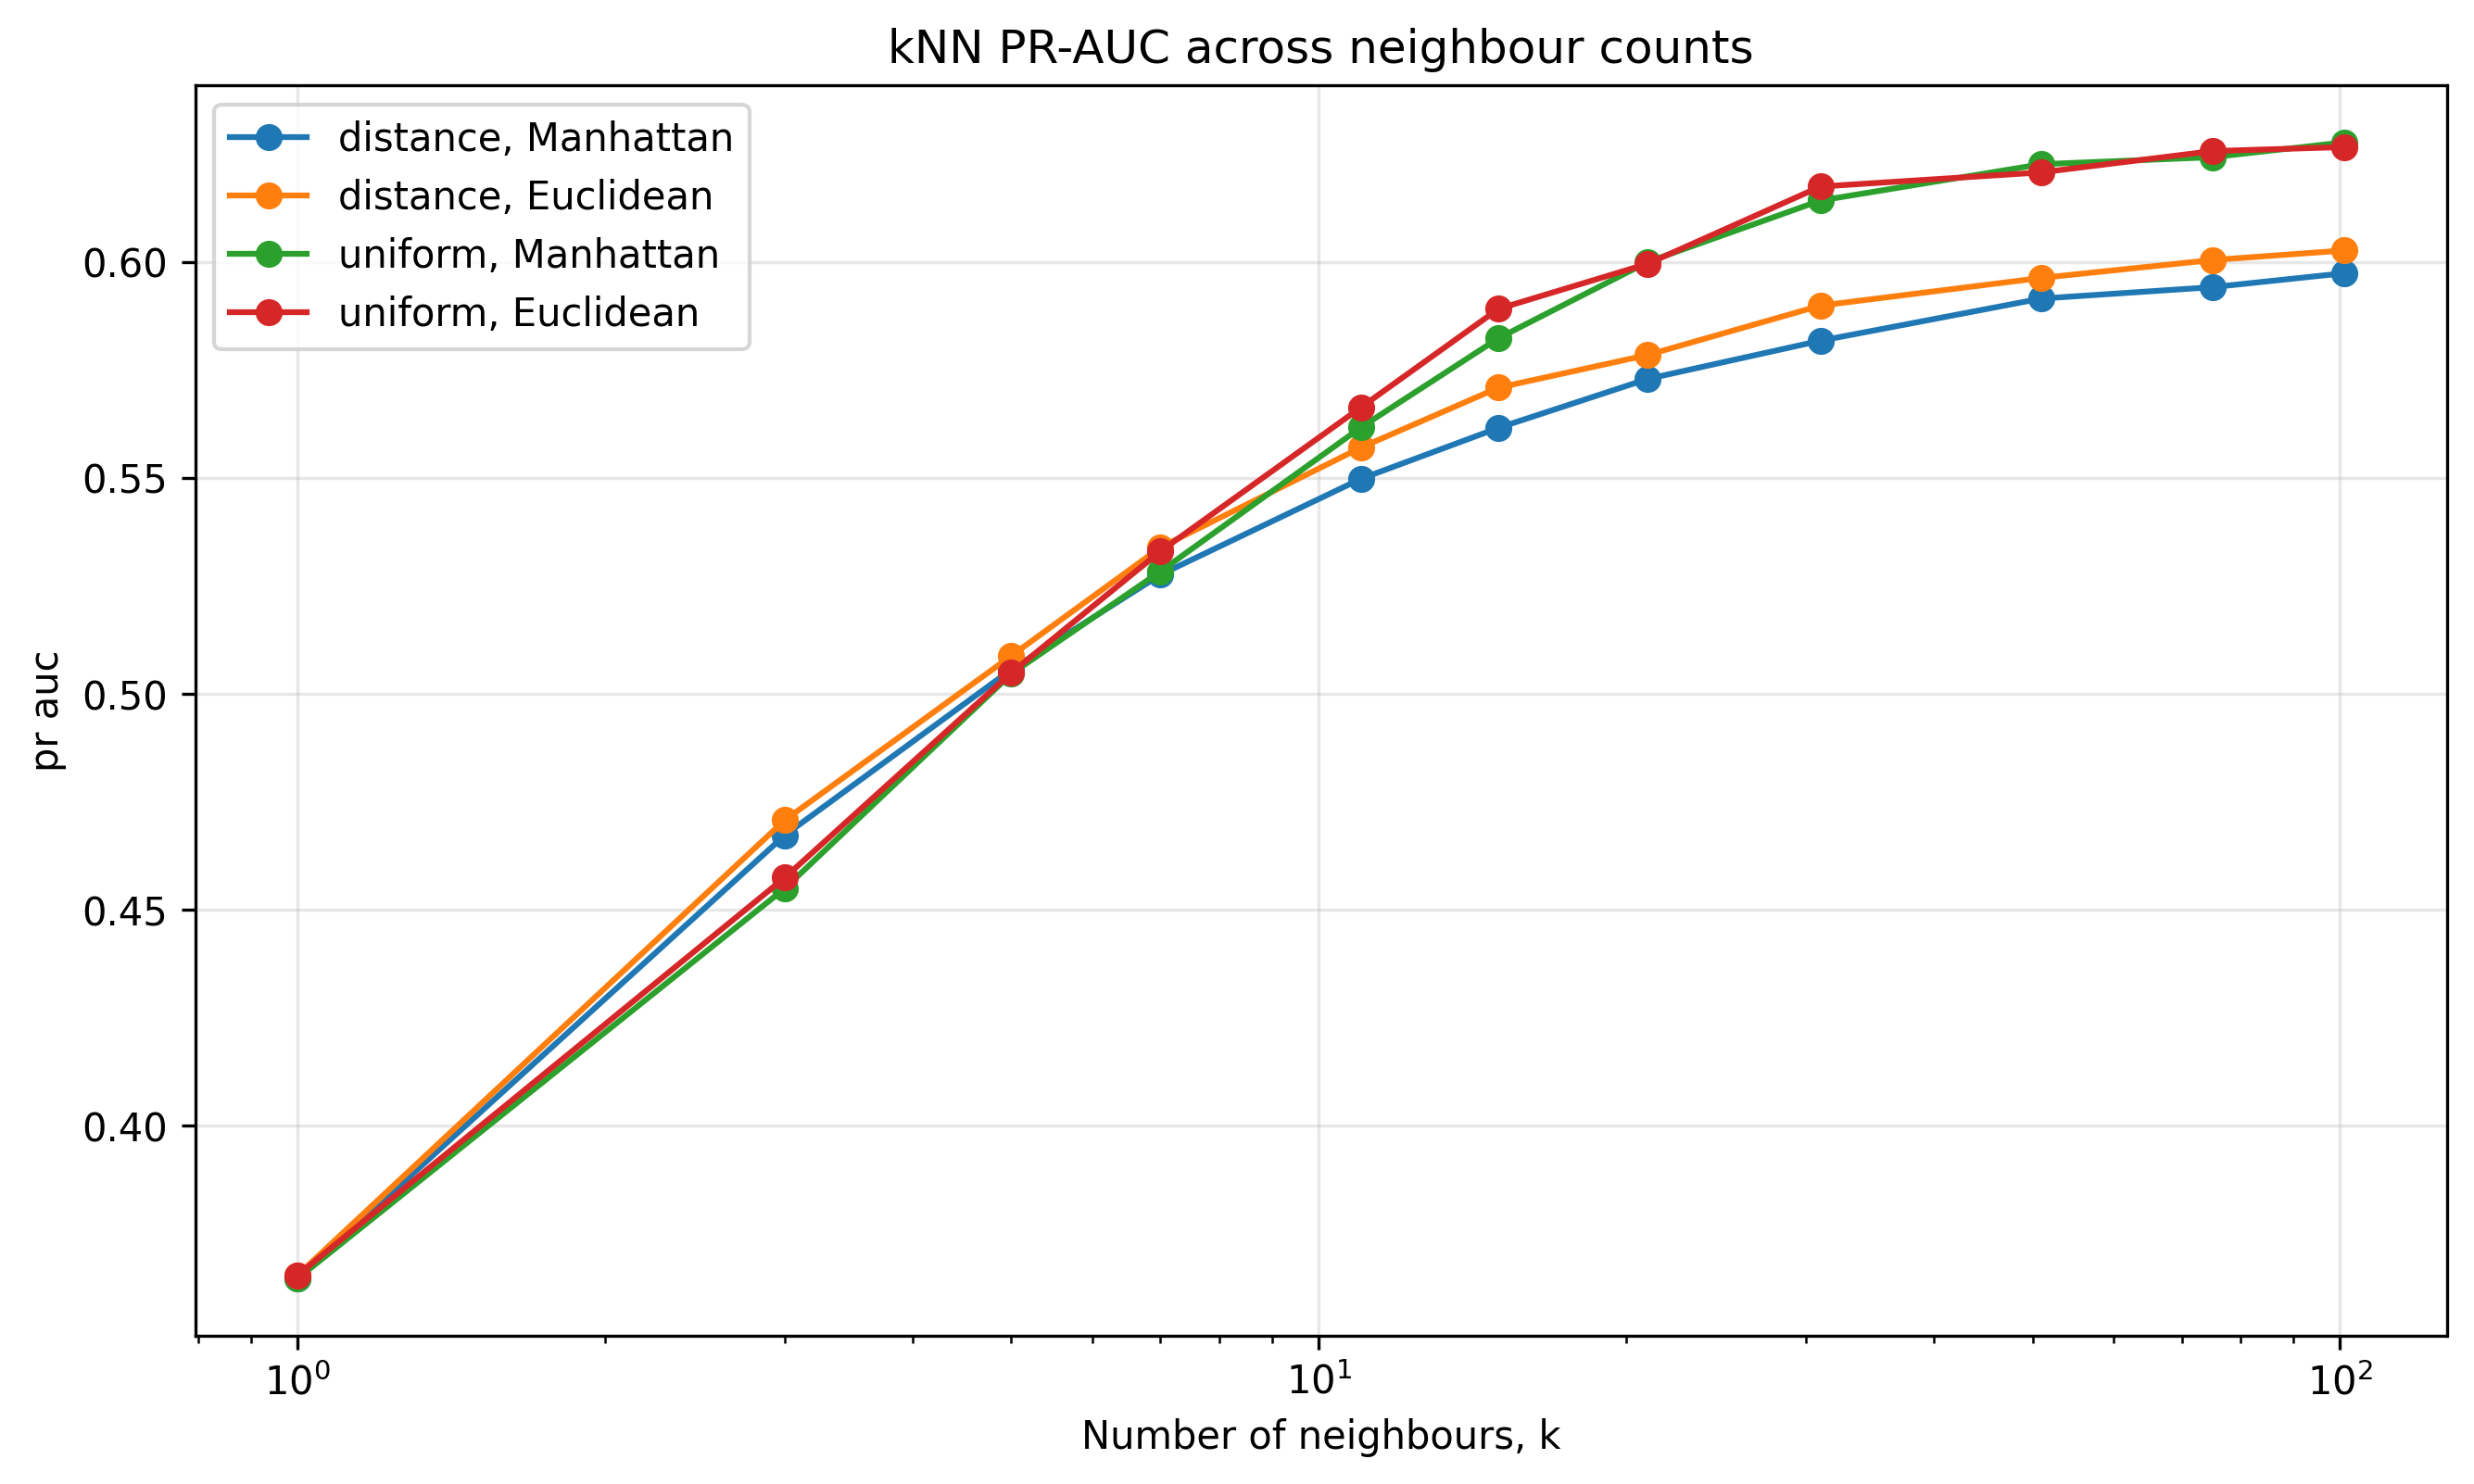
\includegraphics[width=0.88\textwidth]{../figures/knn_pr_auc_by_k.png}
\caption{kNN PR-AUC across neighbour counts}
\label{fig:knn-pr-auc-by-k}
\end{figure}

Figure~\ref{fig:knn-balanced-accuracy-by-k} shows the same grid from the perspective of balanced accuracy. Balanced accuracy also improves as \(k\) increases, but it peaks somewhat earlier than PR-AUC for some configurations. This difference is expected because PR-AUC evaluates ranking quality across thresholds, while balanced accuracy depends on the default hard classification threshold.

\begin{figure}[H]
\centering
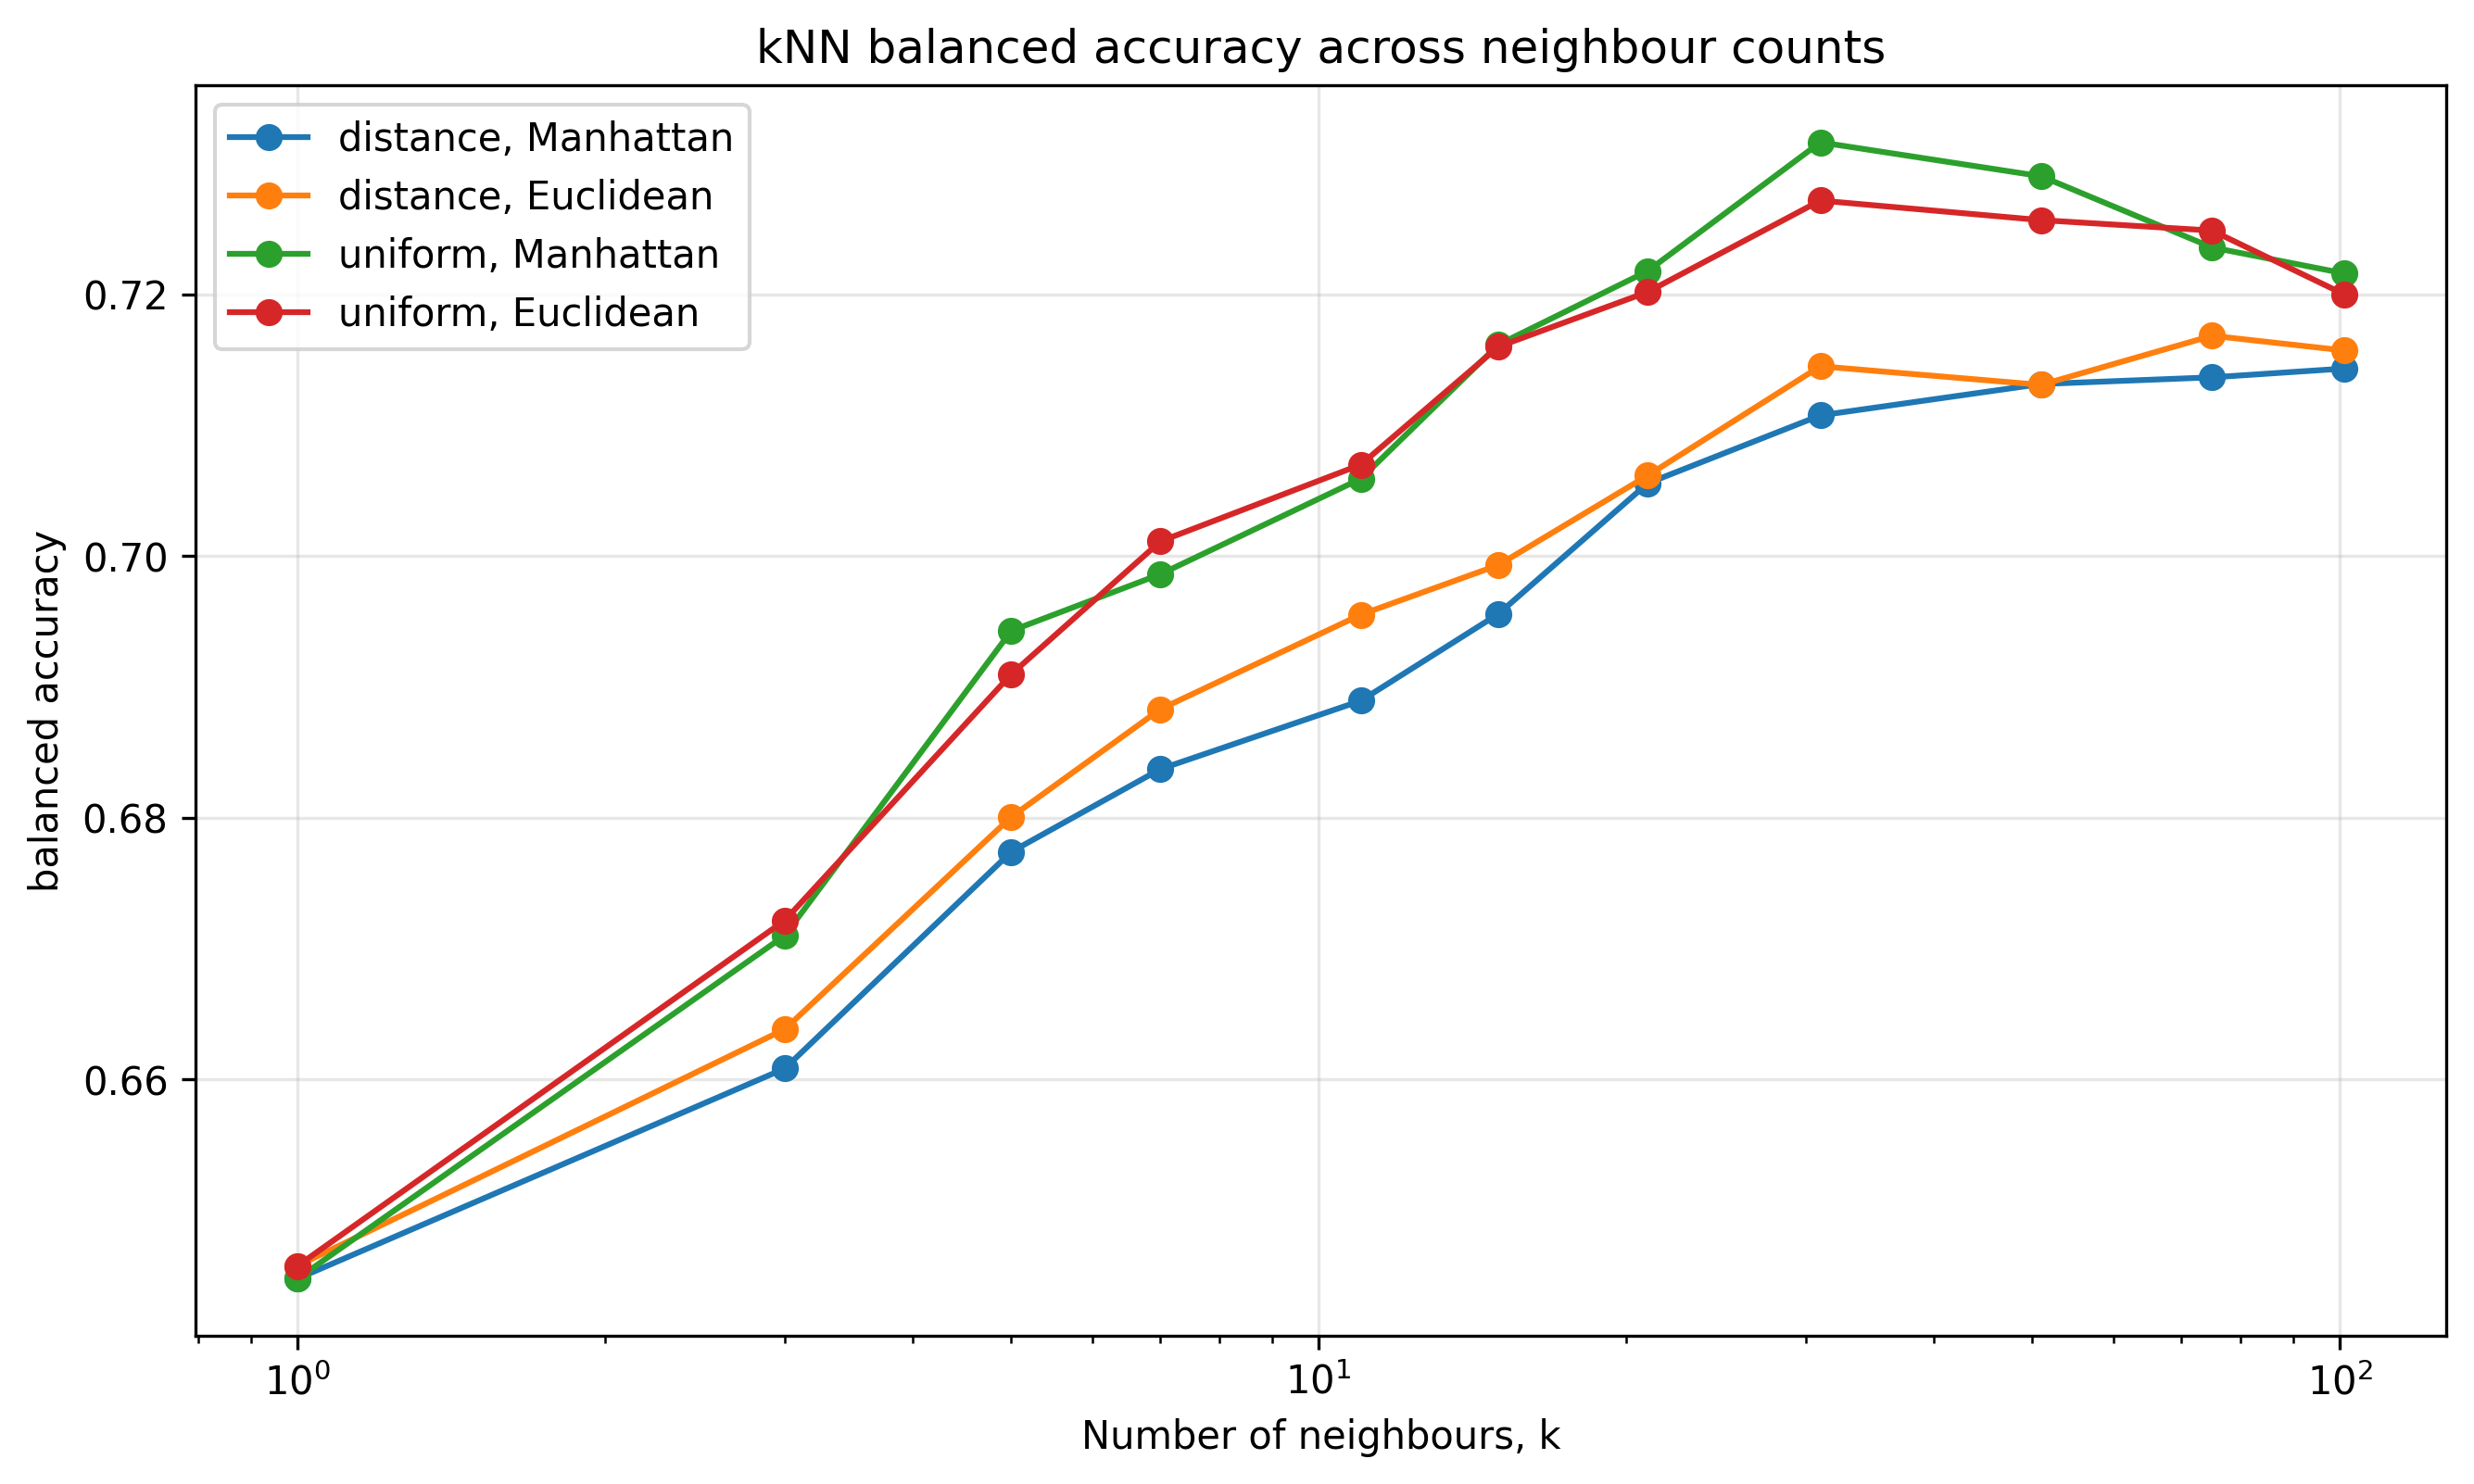
\includegraphics[width=0.88\textwidth]{../figures/knn_balanced_accuracy_by_k.png}
\caption{kNN balanced accuracy across neighbour counts}
\label{fig:knn-balanced-accuracy-by-k}
\end{figure}

The strongest configuration by PR-AUC in the tried grid is the uniform-weighted Manhattan model with \(k=101\). Uniform weighting outperforms distance weighting among the best configurations. This suggests that allowing very close neighbours to dominate does not improve development-stage generalization in this transformed feature space. A smoother average over many neighbours is more stable.

The interpretation should focus on the broader pattern rather than the exact integer \(k=101\). The grid evidence suggests that very small neighbourhoods are too noisy and that larger, smoother neighbourhoods work better for this representation. It does not prove that \(k=101\) is uniquely optimal; nearby large-\(k\) settings may be practically similar.

\subsection{Model comparison}

Table~\ref{tab:knn-model-comparison} compares the default \(k=5\) Euclidean kNN model with the selected kNN model. The selected model improves substantially over the default setting. Accuracy rises from approximately \(0.765\) to \(0.792\), balanced accuracy from approximately \(0.691\) to \(0.722\), ROC-AUC from approximately \(0.782\) to \(0.836\), and PR-AUC from approximately \(0.505\) to \(0.628\). This difference is large enough to support the development-stage conclusion that tuning \(k\), distance, and weighting is important for kNN on this dataset.

\begin{table}[H]
\centering
\small
\begin{tabular}{lrrrrrrrr}
\toprule
Model & Accuracy & Bal. Acc. & Precision & Recall & Specificity & F1 & ROC-AUC & PR-AUC \\
\midrule
Selected kNN, \(k=101\), uniform, Manhattan
& 0.792 & 0.722 & 0.617 & 0.571 & 0.872 & 0.593 & 0.836 & 0.628 \\
kNN, \(k=5\), uniform, Euclidean
& 0.765 & 0.691 & 0.561 & 0.532 & 0.849 & 0.546 & 0.782 & 0.505 \\
\bottomrule
\end{tabular}
\caption{kNN model comparison using cross-validated out-of-fold predictions}
\label{tab:knn-model-comparison}
\end{table}

The corresponding positive-first confusion-matrix counts are shown in Table~\ref{tab:knn-confusion}. The selected model detects more churners and also produces fewer false positives than the default \(k=5\) model. Specifically, the selected model gives \(854\) true positives and \(530\) false positives, compared with \(796\) true positives and \(623\) false positives for the default model.

\begin{table}[H]
\centering
\small
\begin{tabular}{lrrrr}
\toprule
Model & TP & FN & FP & TN \\
\midrule
Selected kNN, \(k=101\), uniform, Manhattan & 854 & 641 & 530 & 3609 \\
kNN, \(k=5\), uniform, Euclidean & 796 & 699 & 623 & 3516 \\
\bottomrule
\end{tabular}
\caption{Positive-first confusion-matrix counts for kNN models}
\label{tab:knn-confusion}
\end{table}

Compared with logistic regression from Section~\ref{sec:linear-classification-and-logistic-regression}, selected kNN has lower development-stage ranking metrics. The selected logistic regression model had ROC-AUC around \(0.846\) and PR-AUC around \(0.658\), while selected kNN has ROC-AUC around \(0.836\) and PR-AUC around \(0.628\). This suggests that the global feature-weighting structure learned by logistic regression is more effective than direct distance-based local similarity for this transformed Telco churn dataset.

This comparison should still be read as development-stage evidence. The gap is meaningful enough to keep logistic regression as the stronger candidate so far, but final statistical claims about model-family superiority are deferred to the later model-comparison and test-evaluation stages.

\subsection{Threshold behaviour}

The selected kNN model provides predicted probabilities from neighbour proportions. Figure~\ref{fig:knn-threshold-tradeoff} shows how precision, recall, specificity, and F1 change as the classification threshold varies. Lower thresholds identify many more churners but also flag many more non-churners. Higher thresholds improve precision and specificity but miss more churners.

\begin{figure}[H]
\centering
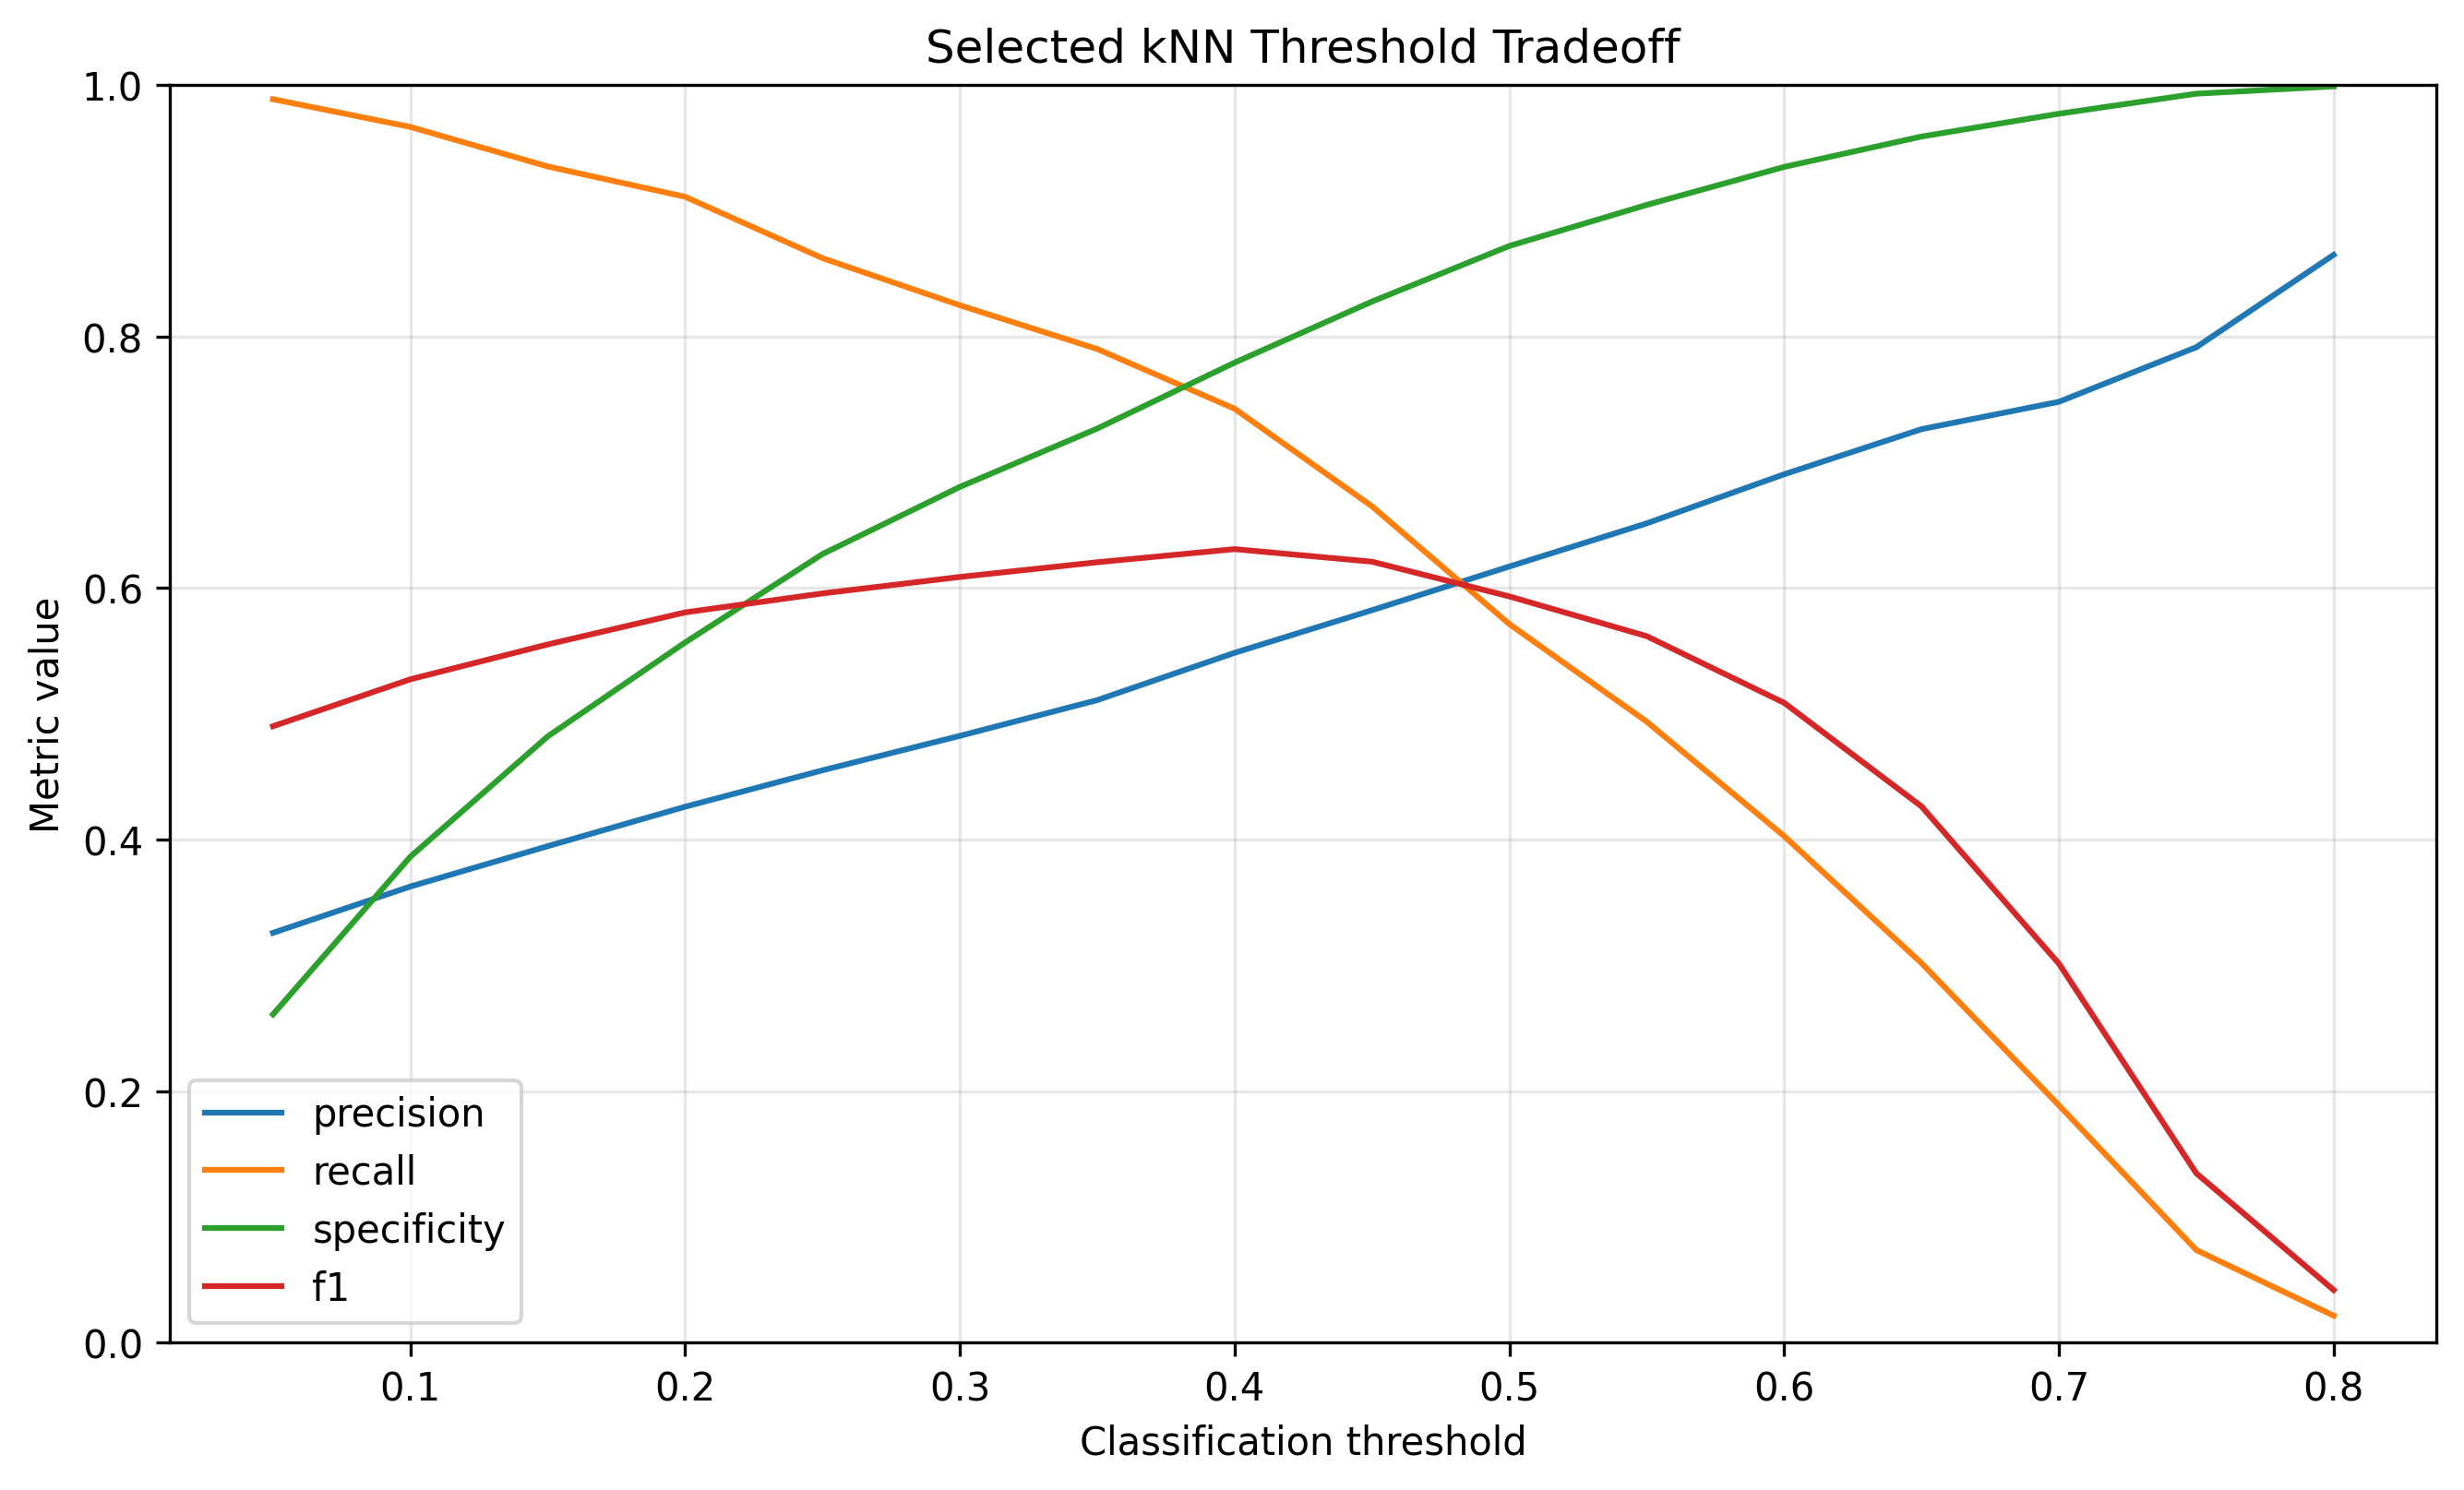
\includegraphics[width=0.88\textwidth]{../figures/knn_threshold_tradeoff.png}
\caption{Threshold tradeoff for the selected kNN model}
\label{fig:knn-threshold-tradeoff}
\end{figure}

At threshold \(0.25\), recall is approximately \(0.862\), but precision is only approximately \(0.455\). At threshold \(0.40\), the model reaches a more balanced operating point, with precision approximately \(0.548\), recall approximately \(0.742\), specificity approximately \(0.779\), and F1 approximately \(0.631\). At the default threshold \(0.50\), precision improves to approximately \(0.617\), but recall falls to approximately \(0.571\). This again shows that threshold \(0.50\) is not necessarily the best operating point for churn detection.

These threshold results are diagnostic rather than final. Threshold selection is itself a modelling decision and is postponed until the later model-comparison stage, where the project objective and candidate model families can be considered together.

\subsection{ROC and precision-recall curves}

Figure~\ref{fig:knn-roc-curve} shows the ROC curve for the selected kNN model. The ROC-AUC is approximately \(0.836\), clearly above the random-ranking line. This indicates that the selected kNN model ranks churners above non-churners much better than chance.

\begin{figure}[H]
\centering
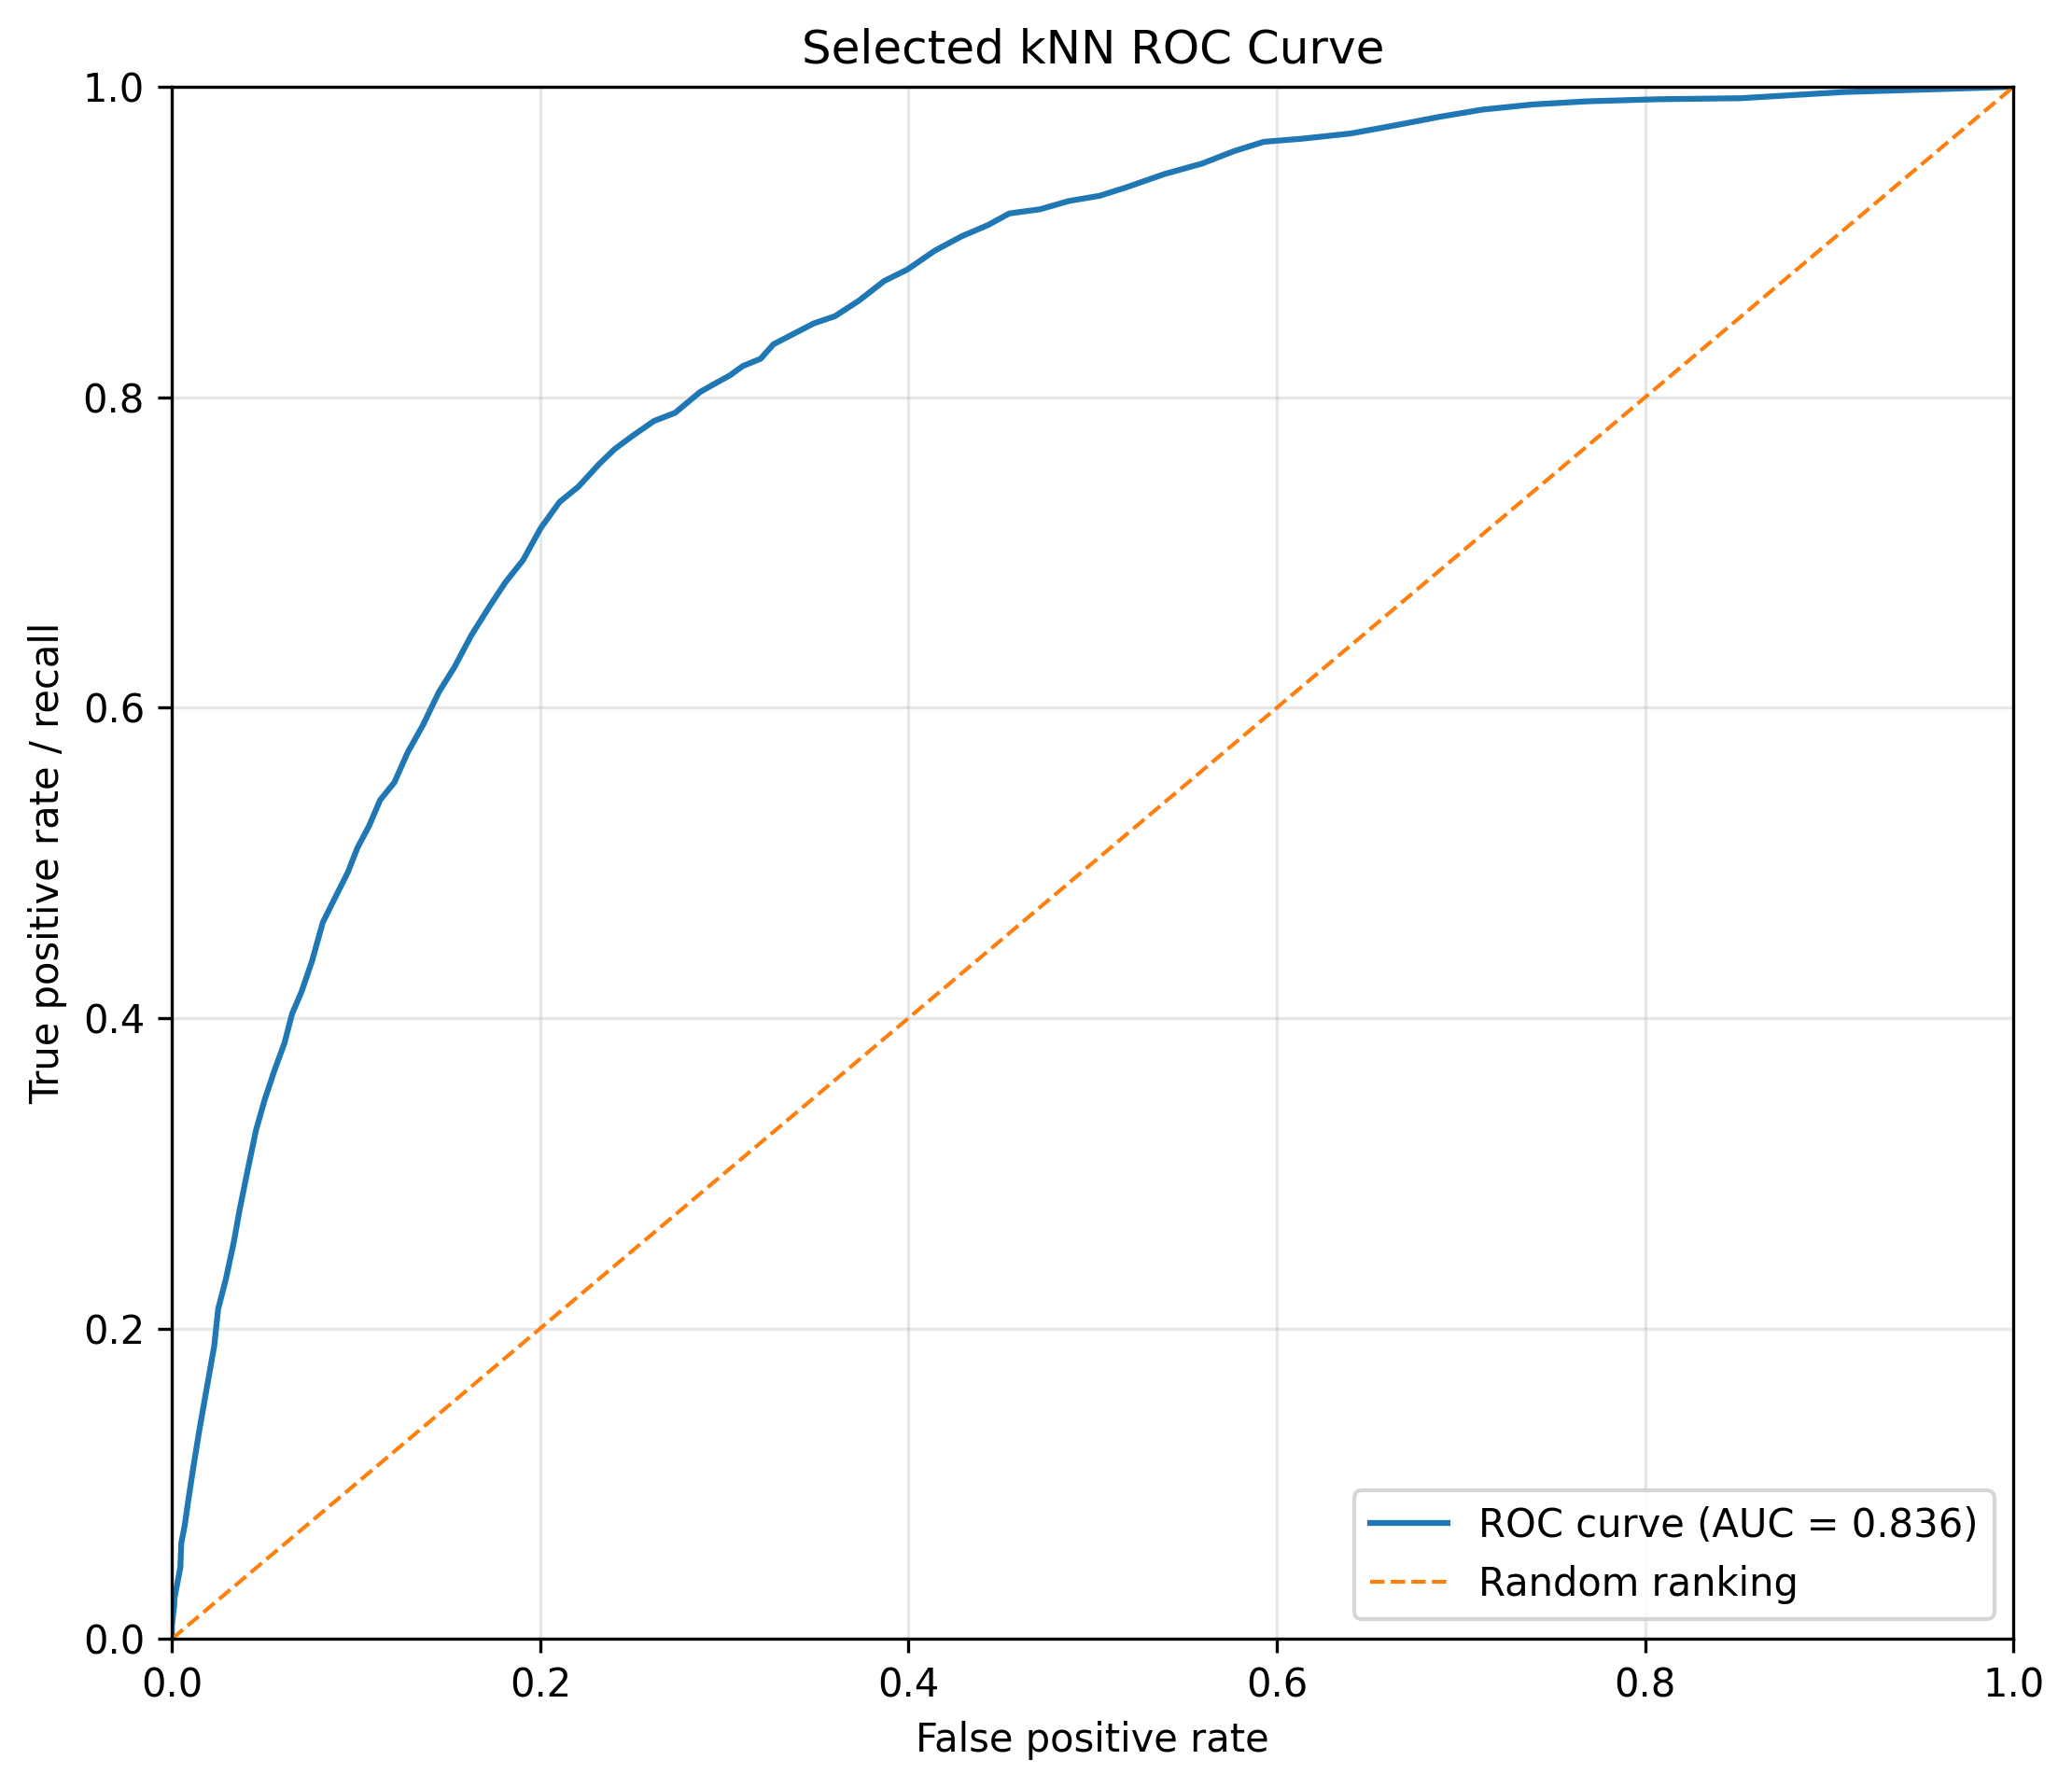
\includegraphics[width=0.72\textwidth]{../figures/knn_roc_curve.png}
\caption{ROC curve for the selected kNN model}
\label{fig:knn-roc-curve}
\end{figure}

Figure~\ref{fig:knn-pr-curve} shows the precision-recall curve. The PR-AUC is approximately \(0.631\), well above the positive-rate baseline of approximately \(0.265\). This confirms that kNN has useful positive-class retrieval ability. However, it remains below the logistic regression PR-AUC from Section~\ref{sec:linear-classification-and-logistic-regression}. The gap is not extremely large, so it should be interpreted as development-stage evidence rather than final statistical proof.

\begin{figure}[H]
\centering
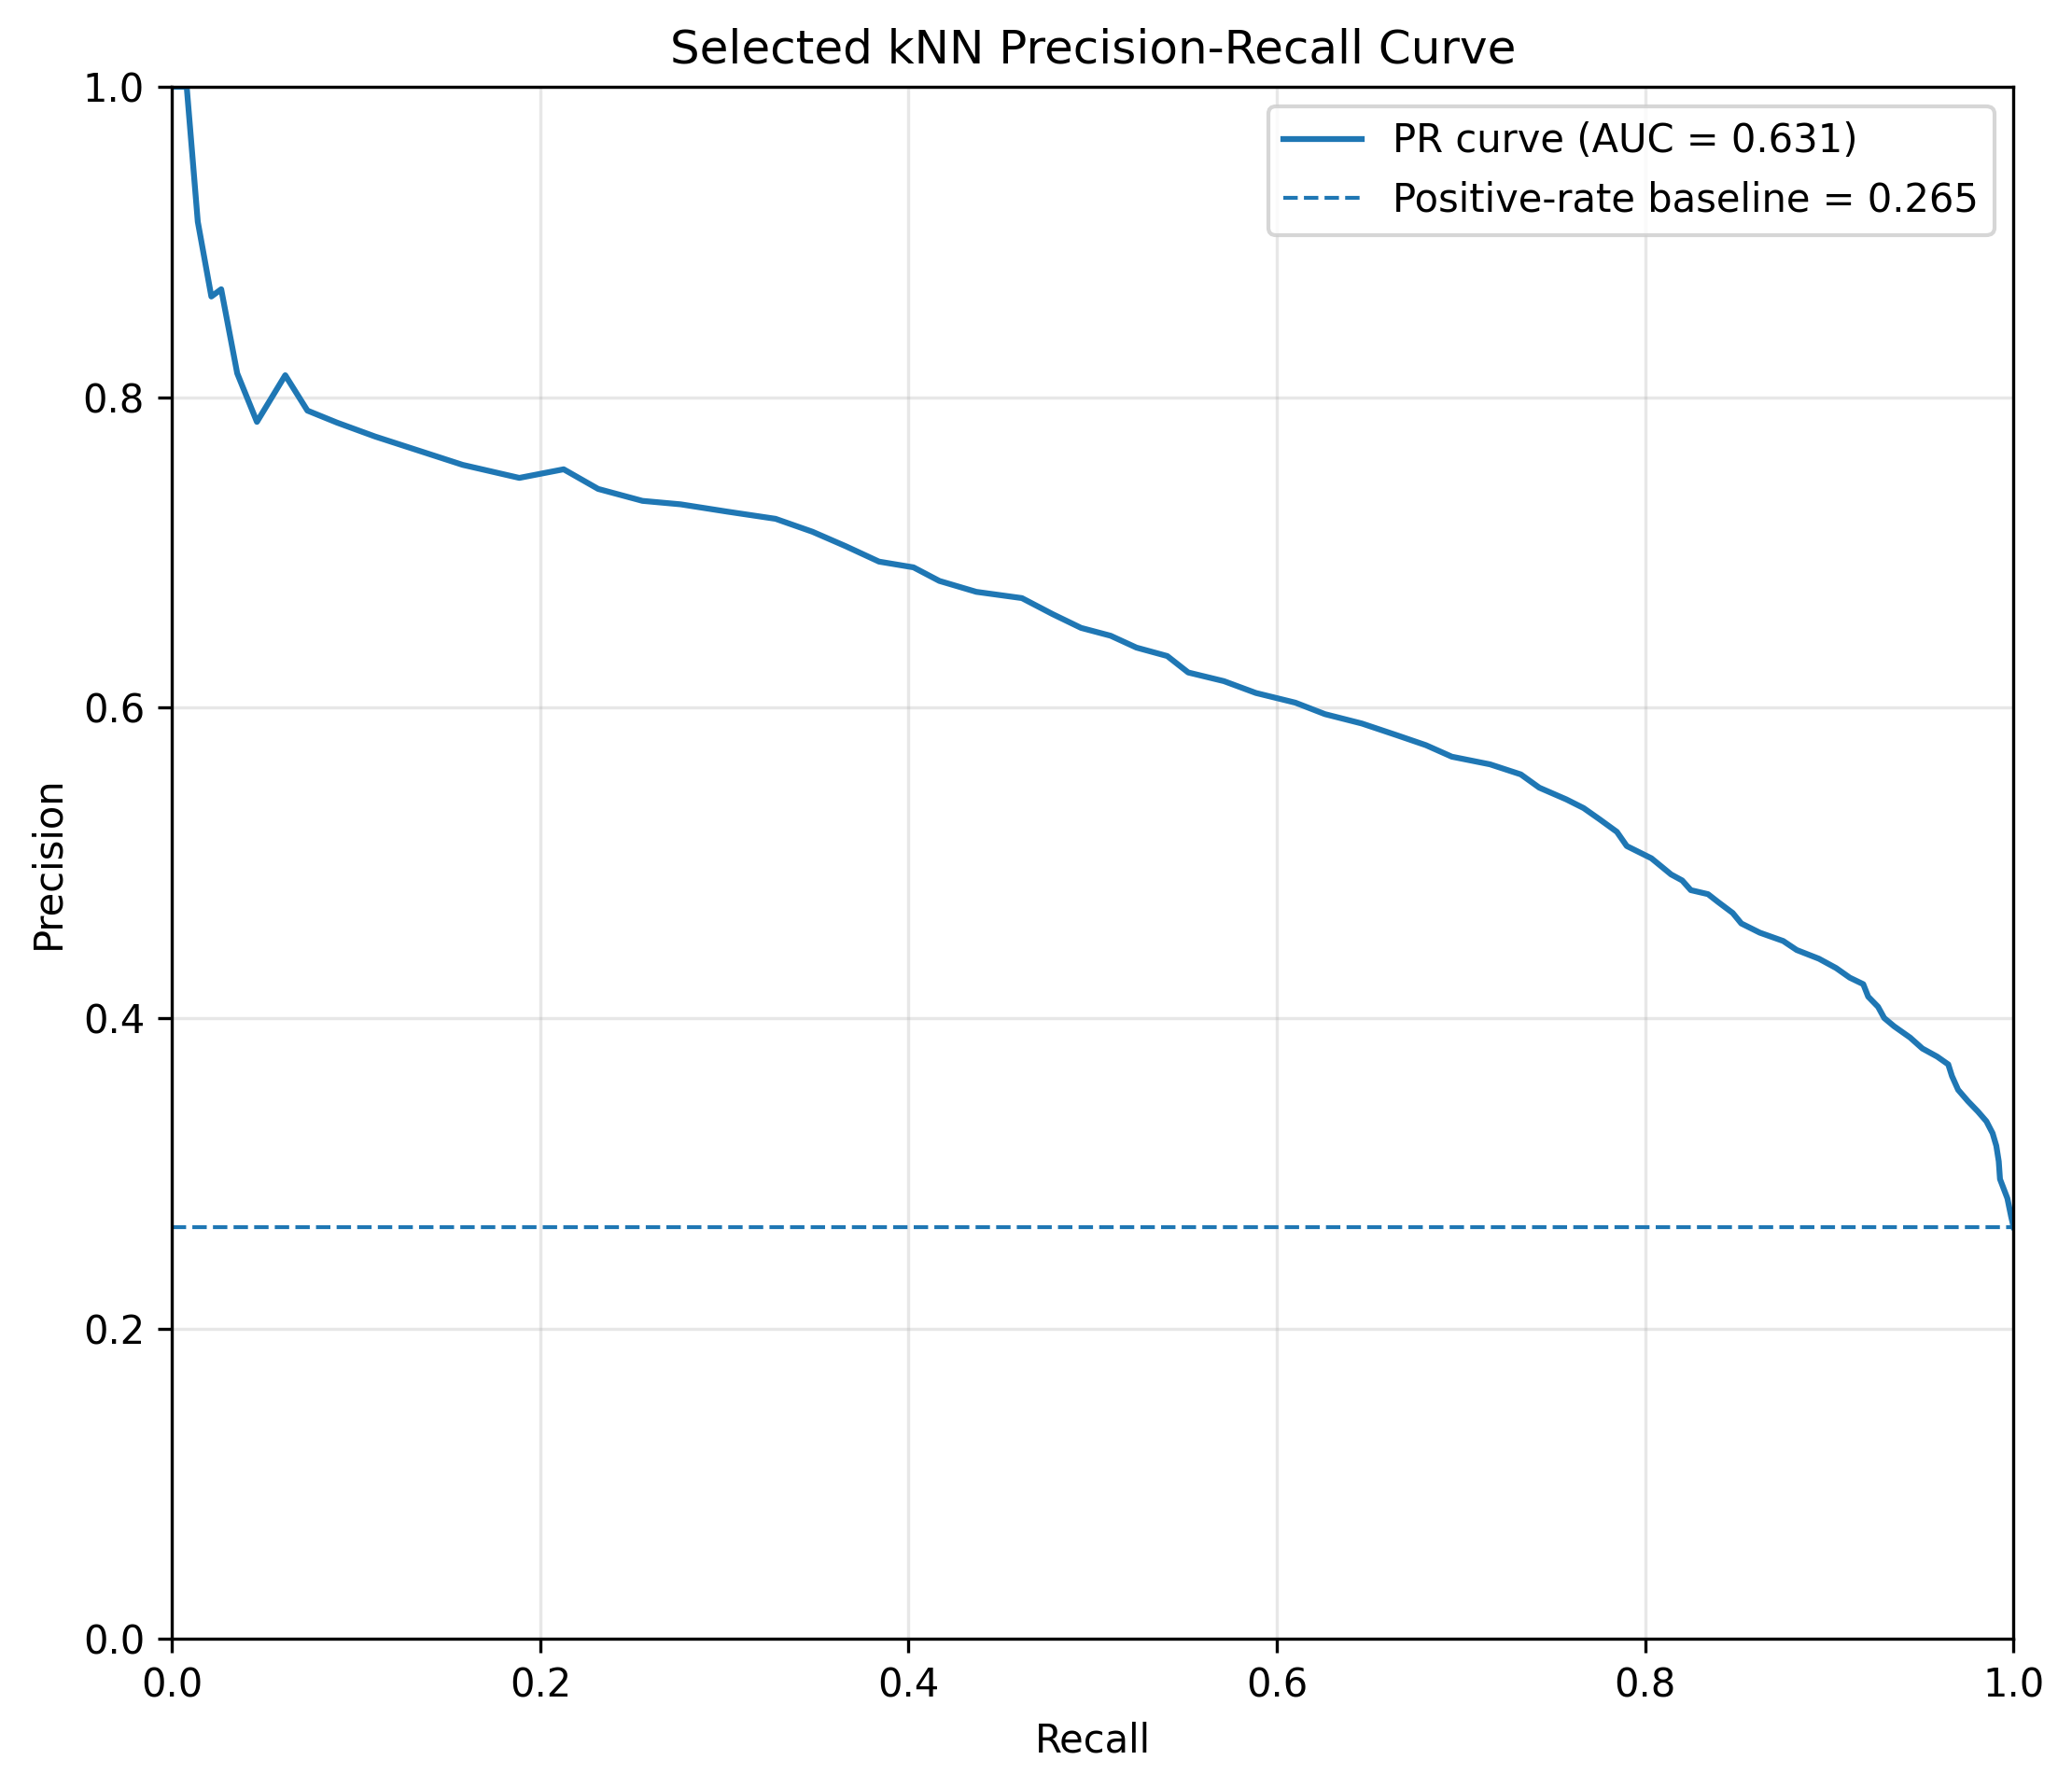
\includegraphics[width=0.72\textwidth]{../figures/knn_precision_recall_curve.png}
\caption{Precision-recall curve for the selected kNN model}
\label{fig:knn-pr-curve}
\end{figure}

\subsection{Summary}

The k-nearest-neighbour experiment shows that distance-based classification learns meaningful churn structure, but it does not outperform logistic regression in the current development-stage comparison. The most important findings are as follows. First, kNN performance is highly sensitive to the number of neighbours. Small \(k\) values are too noisy, while larger neighbourhoods perform better. Second, uniform weighting works better than distance weighting in the strongest configurations. Third, the strongest PR-AUC in the grid is obtained by the uniform Manhattan model with \(k=101\), which is a relatively smooth kNN classifier. Fourth, the selected kNN model improves substantially over the default \(k=5\) baseline, but remains below logistic regression in ROC-AUC and PR-AUC.

The section is useful because it introduces local, distance-based learning and the bias-variance role of \(k\). It also illustrates a limitation of distance-based methods on one-hot encoded tabular data: the constructed distance space may not be as informative as a model that learns feature weights directly. The exact selected \(k\) should not be overinterpreted; the robust lesson is that smoothing over a larger neighbourhood is preferable to very local neighbour voting for this feature representation. The next modelling stage introduces Naive Bayes before the project moves to tree-based models.


\newpage
\newpage
\section{Naive Bayes}
\label{sec:naive-bayes}

This section evaluates Naive Bayes classifiers as the first explicitly generative model family in the project. Logistic regression directly models the posterior probability \(P(Y=1\mid X=x)\), and k-nearest neighbours predicts from local similarity in the transformed feature space. Naive Bayes instead models the class prior and the feature distribution within each class, then applies Bayes' rule to obtain posterior class probabilities.

The same training-only validation discipline is used as in the previous modelling sections. The held-out test set remains unused. All reported results are based on stratified cross-validation inside the training set, using out-of-fold predictions.

\subsection{Bayes classifier}

For binary classification, the ideal classifier predicts the class with the largest true posterior probability:
\[
h^\star(x)
=
\arg\max_{y\in\{0,1\}}
P(Y=y\mid X=x).
\]
For churn classification, where \(Y=1\) denotes churn and \(Y=0\) denotes no churn, this can be written as
\[
h^\star(x)
=
\mathbb{1}
\left\{
P(Y=1\mid X=x)\geq 0.5
\right\}.
\]
This rule is called the Bayes classifier. It is ideal because it uses the true conditional probability of the class given the features. In practice, this posterior probability is unknown and must be estimated from data.

Under 0-1 loss, the risk of a classifier \(h\) is
\[
R(h)
=
P(h(X)\neq Y)
=
\mathbb{E}
\left[
\mathbb{1}\{h(X)\neq Y\}
\right].
\]
The Bayes classifier minimizes this risk over all possible classifiers:
\[
h^\star
=
\arg\min_h R(h).
\]
The corresponding minimum possible error rate is the Bayes risk,
\[
R^\star
=
R(h^\star).
\]
For binary classification, the Bayes risk can be written as
\[
R^\star
=
\mathbb{E}_X
\left[
\min
\{
P(Y=0\mid X),
P(Y=1\mid X)
\}
\right].
\]
This expression shows that classification error can be irreducible. If churners and non-churners overlap for the same observed feature values, then even the ideal classifier must sometimes be wrong.

\subsection{Bayes decision rule and unequal costs}

The threshold \(0.5\) is optimal only when false positives and false negatives have equal cost. In churn prediction, this is not necessarily realistic. A false positive may cause unnecessary retention effort, while a false negative may mean missing a customer who will leave.

Let \(C_{\mathrm{FP}}\) denote the cost of a false positive and \(C_{\mathrm{FN}}\) the cost of a false negative. A cost-sensitive Bayes decision rule predicts churn when
\[
C_{\mathrm{FP}}P(Y=0\mid X=x)
\leq
C_{\mathrm{FN}}P(Y=1\mid X=x).
\]
Equivalently, predict churn when
\[
P(Y=1\mid X=x)
\geq
\frac{C_{\mathrm{FP}}}{C_{\mathrm{FP}}+C_{\mathrm{FN}}}.
\]
If missing a churner is more costly than unnecessarily contacting a non-churner, then \(C_{\mathrm{FN}}>C_{\mathrm{FP}}\), and the optimal threshold is below \(0.5\). This provides the theoretical reason why the project studies threshold tradeoffs for probabilistic classifiers.

\subsection{Bayes' rule and generative classification}

Bayes' rule gives
\[
P(Y=y\mid X=x)
=
\frac{
P(X=x\mid Y=y)P(Y=y)
}{
P(X=x)
}.
\]
For classification, the denominator \(P(X=x)\) is the same for every class. Therefore, the predicted class can be obtained by comparing the unnormalized posterior scores:
\[
\widehat{y}
=
\arg\max_{y\in\{0,1\}}
P(X=x\mid Y=y)P(Y=y).
\]
The term \(P(Y=y)\) is the class prior. The term \(P(X=x\mid Y=y)\) is the class-conditional feature likelihood.

Naive Bayes is a generative classifier because it models \(P(Y)\) and \(P(X\mid Y)\). Conceptually, the model describes a process in which a class is first drawn from the class prior, and features are then drawn from the class-conditional feature distribution.

\subsection{The naive conditional-independence assumption}

The full class-conditional feature distribution is
\[
P(X=x\mid Y=y)
=
P(X_1=x_1,\ldots,X_p=x_p\mid Y=y).
\]
Estimating this full joint distribution is difficult when the feature vector is high-dimensional. Naive Bayes makes the simplifying assumption that features are conditionally independent given the class:
\[
P(X=x\mid Y=y)
=
\prod_{j=1}^{p}
P(X_j=x_j\mid Y=y).
\]
The posterior score is therefore proportional to
\[
P(Y=y)
\prod_{j=1}^{p}
P(X_j=x_j\mid Y=y).
\]
In practice, computations are done on the log scale:
\[
\log P(Y=y)
+
\sum_{j=1}^{p}
\log P(X_j=x_j\mid Y=y).
\]
This avoids numerical underflow and turns a product of probabilities into a sum of feature-level log-likelihood contributions.

The independence assumption is not literally true for this dataset. For example, \texttt{tenure} and \texttt{TotalCharges} are strongly related, and the internet-service variables are structurally connected to service add-ons such as \texttt{OnlineSecurity}, \texttt{OnlineBackup}, and \texttt{TechSupport}. Therefore, Naive Bayes may double-count related evidence and produce overconfident probabilities. Nevertheless, it can still be useful as a classifier if the posterior ranking remains informative.

\subsection{Naive Bayes variants}

This section evaluates three transparent Naive Bayes variants.

First, Gaussian Naive Bayes is applied to the numeric features only. Gaussian Naive Bayes assumes
\[
X_j\mid Y=y
\sim
\mathcal{N}(\mu_{jy},\sigma_{jy}^{2}),
\]
with class-specific means and variances. This model uses only \texttt{tenure}, \texttt{MonthlyCharges}, and \texttt{TotalCharges}.

Second, Bernoulli Naive Bayes is applied to one-hot encoded categorical features only. For a binary indicator \(X_j\in\{0,1\}\), Bernoulli Naive Bayes uses
\[
P(X_j=x_j\mid Y=y)
=
\theta_{jy}^{x_j}(1-\theta_{jy})^{1-x_j}.
\]
Additive smoothing is used to avoid zero probabilities. With smoothing parameter \(\alpha\), estimated probabilities are pulled away from exactly zero and one.

Third, Gaussian Naive Bayes is applied to the full transformed feature matrix, including numeric variables and one-hot encoded categorical indicators. This is not the cleanest theoretical likelihood for binary indicators, but it provides a simple full-feature generative baseline.

\subsection{Model comparison}

Table~\ref{tab:nb-model-comparison} reports the cross-validated results for the three main Naive Bayes variants. The selected model by PR-AUC is the full transformed Gaussian Naive Bayes model. It has PR-AUC approximately \(0.605\), ROC-AUC approximately \(0.819\), and recall approximately \(0.847\). The categorical-only Bernoulli model has slightly better balanced accuracy and \(F_1\), but its PR-AUC is lower. The numeric-only Gaussian model has higher ordinary accuracy, but substantially lower recall.

\begin{table}[H]
\centering
\small
\resizebox{\textwidth}{!}{
\begin{tabular}{lrrrrrrrr}
\toprule
Model & Accuracy & Bal. Acc. & Precision & Recall & Specificity & \(F_1\) & ROC-AUC & PR-AUC \\
\midrule
GaussianNB full transformed & 0.698 & 0.746 & 0.462 & 0.847 & 0.644 & 0.598 & 0.819 & 0.605 \\
BernoulliNB categorical only, \(\alpha=1\) & 0.721 & 0.751 & 0.485 & 0.814 & 0.687 & 0.608 & 0.815 & 0.596 \\
GaussianNB numeric only & 0.764 & 0.696 & 0.557 & 0.549 & 0.842 & 0.553 & 0.774 & 0.584 \\
\bottomrule
\end{tabular}
}
\caption{Cross-validated Naive Bayes model comparison on the training set}
\label{tab:nb-model-comparison}
\end{table}

The corresponding confusion-matrix counts are shown in Table~\ref{tab:nb-confusion}. The selected full transformed Gaussian model detects \(1267\) of the \(1495\) churners, but also flags \(1475\) non-churners as churners. This confirms that the selected Naive Bayes model is a high-recall, high-alert-rate model at the default threshold.

\begin{table}[H]
\centering
\small
\begin{tabular}{lrrrr}
\toprule
Model & TP & FN & FP & TN \\
\midrule
GaussianNB full transformed & 1267 & 228 & 1475 & 2664 \\
BernoulliNB categorical only, \(\alpha=1\) & 1217 & 278 & 1294 & 2845 \\
GaussianNB numeric only & 821 & 674 & 653 & 3486 \\
\bottomrule
\end{tabular}
\caption{Positive-first confusion-matrix counts for Naive Bayes models}
\label{tab:nb-confusion}
\end{table}

Compared with logistic regression and k-nearest neighbours, Naive Bayes is more aggressive in predicting churn. The selected Naive Bayes model has recall around \(0.847\), much higher than the default-threshold recall of the selected logistic and kNN models. However, this comes at the cost of weaker precision and specificity. Its ranking metrics are also lower: ROC-AUC is about \(0.819\) and PR-AUC is about \(0.605\), compared with approximately \(0.846\) and \(0.658\) for selected logistic regression, and approximately \(0.836\) and \(0.628\) for selected kNN.

\subsection{Smoothing sensitivity for Bernoulli Naive Bayes}

Figure~\ref{fig:bernoulli-nb-alpha} shows the Bernoulli Naive Bayes smoothing experiment. The metrics are almost flat across the tested range of \(\alpha\). This means that additive smoothing is not a major source of performance variation for this dataset and feature representation.

\begin{figure}[H]
\centering
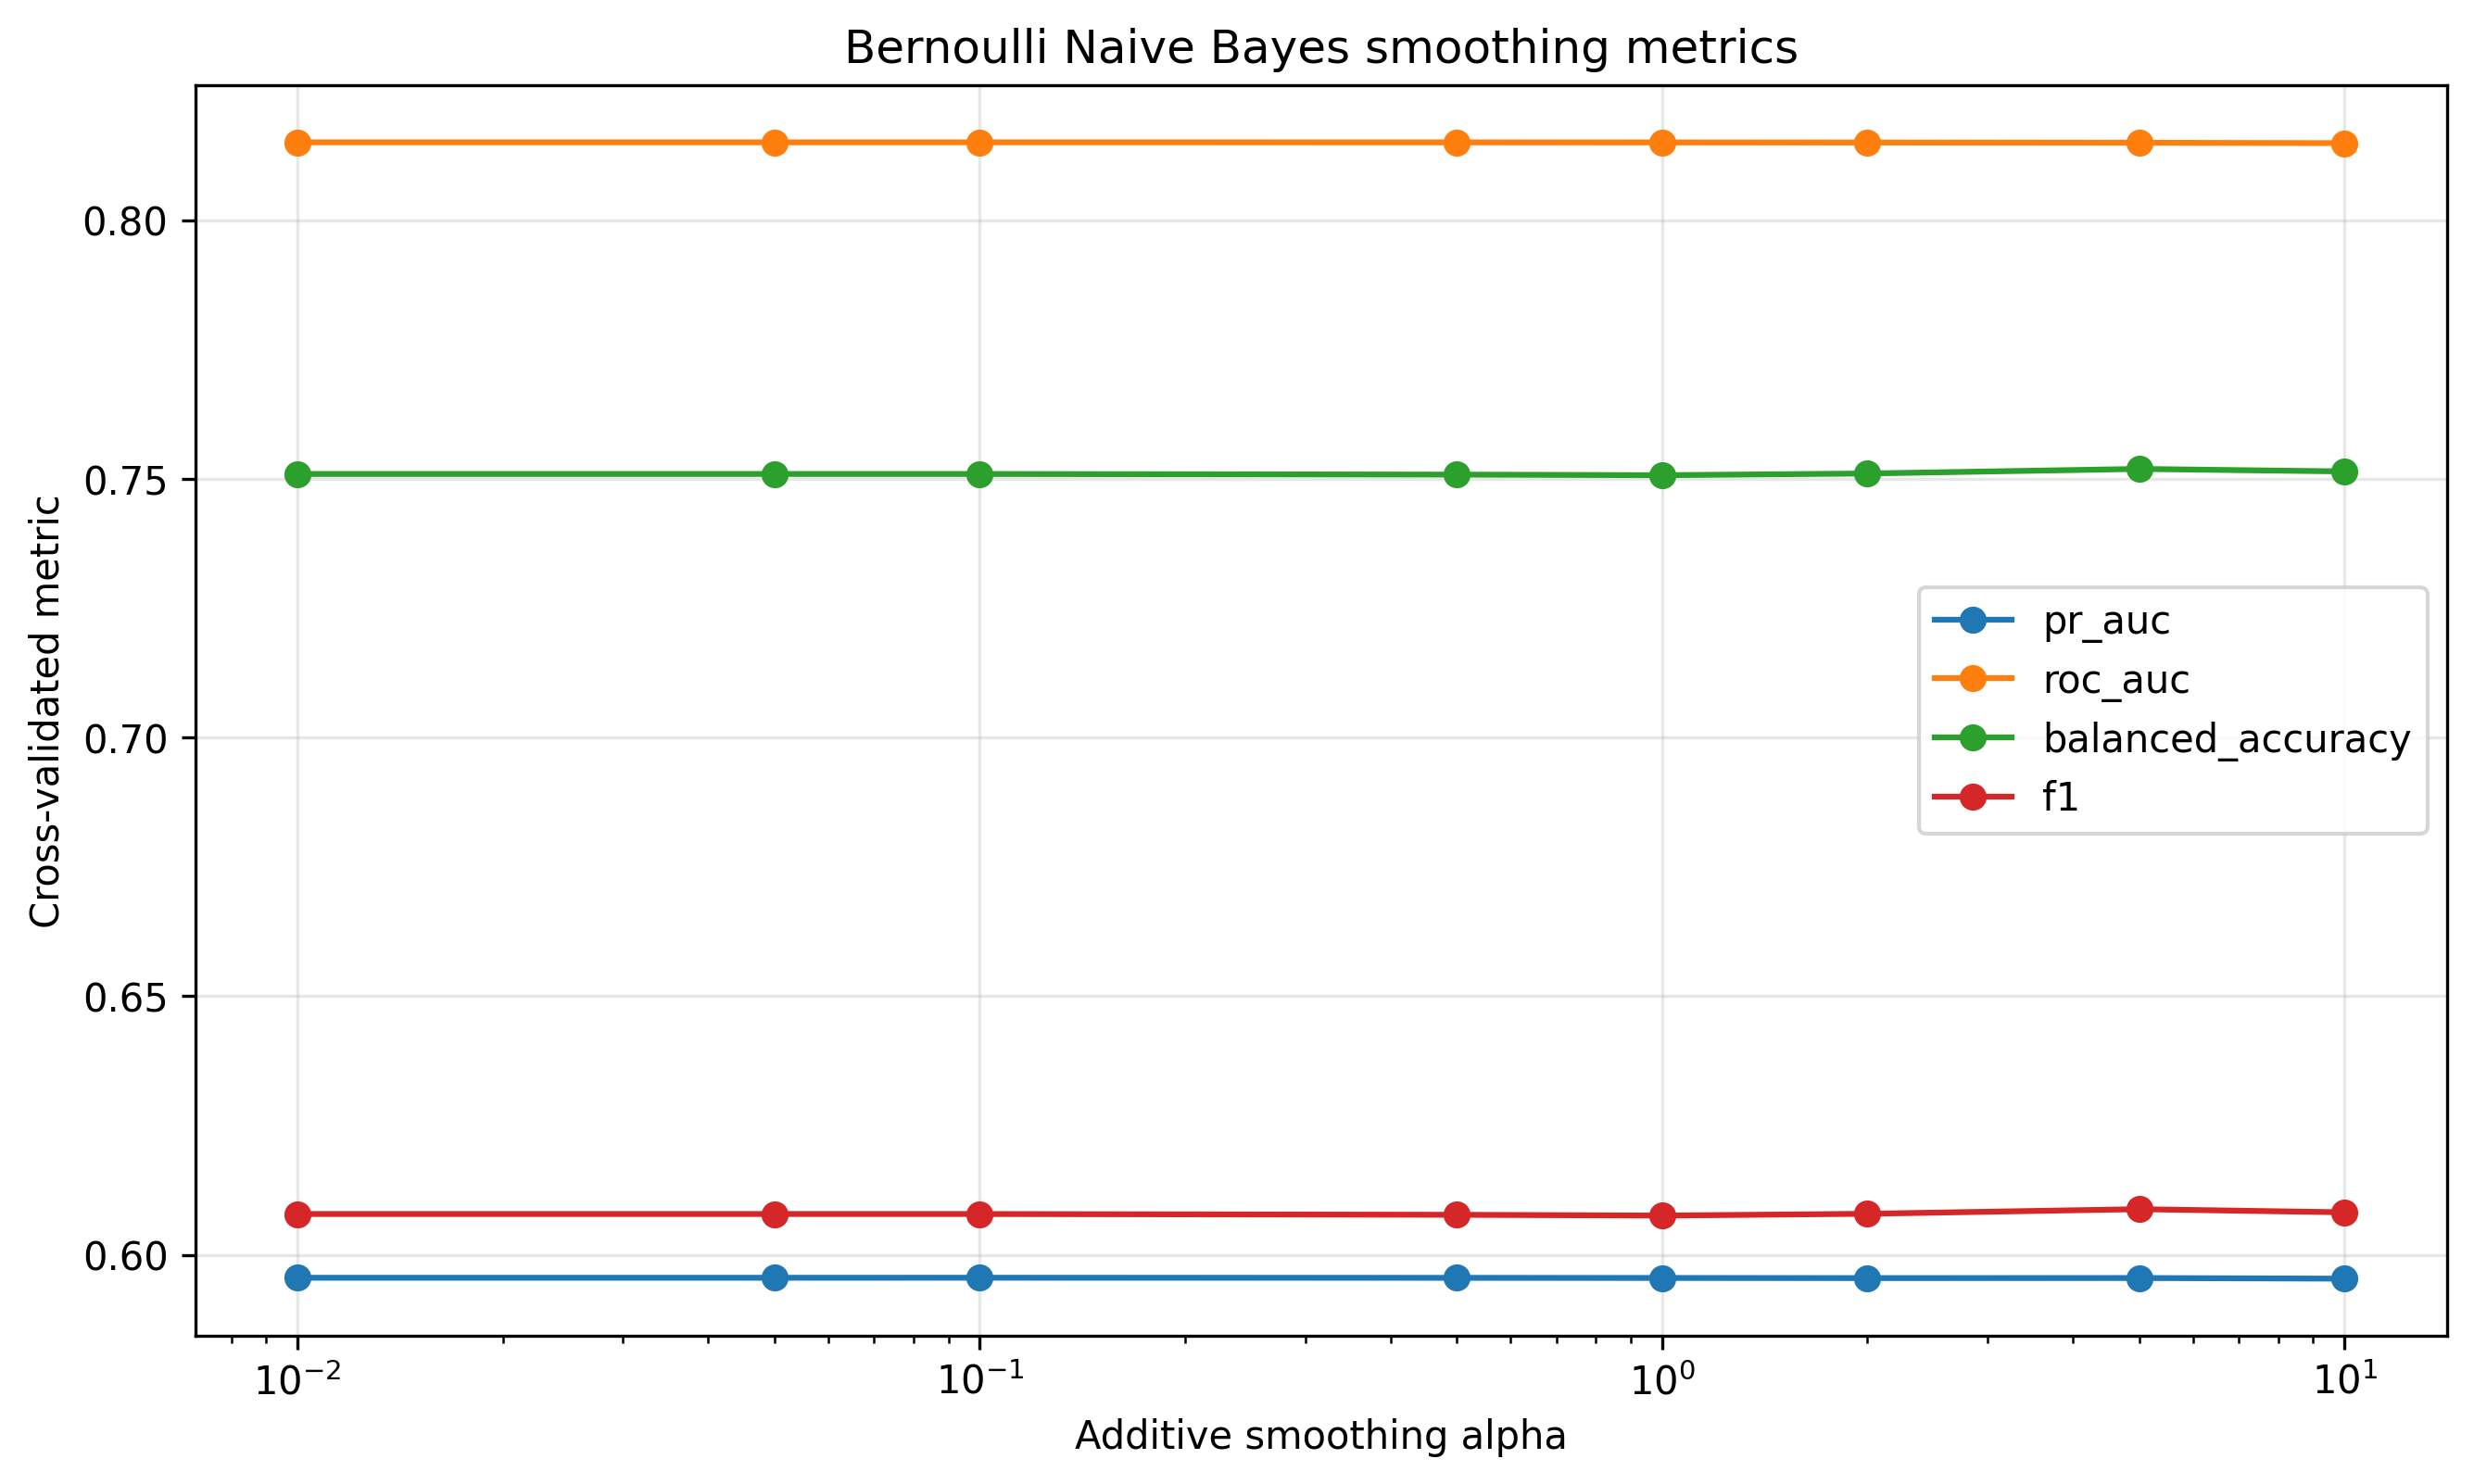
\includegraphics[width=0.82\textwidth]{../figures/bernoulli_nb_alpha_metrics.png}
\caption{Bernoulli Naive Bayes smoothing metrics}
\label{fig:bernoulli-nb-alpha}
\end{figure}

For example, PR-AUC remains around \(0.596\) across the grid, ROC-AUC remains around \(0.815\), and balanced accuracy remains close to \(0.751\). This stability suggests that the categorical indicator likelihoods are not overly sensitive to rare zero-probability problems under this cross-validation setup.

\subsection{Threshold behaviour}

Figure~\ref{fig:nb-threshold-tradeoff} shows the threshold tradeoff for the selected full transformed Gaussian Naive Bayes model. The curve is strikingly flat compared with the threshold curves for logistic regression and kNN. Even when the threshold increases from \(0.05\) to \(0.80\), recall remains high, while precision increases only gradually.

\begin{figure}[H]
\centering
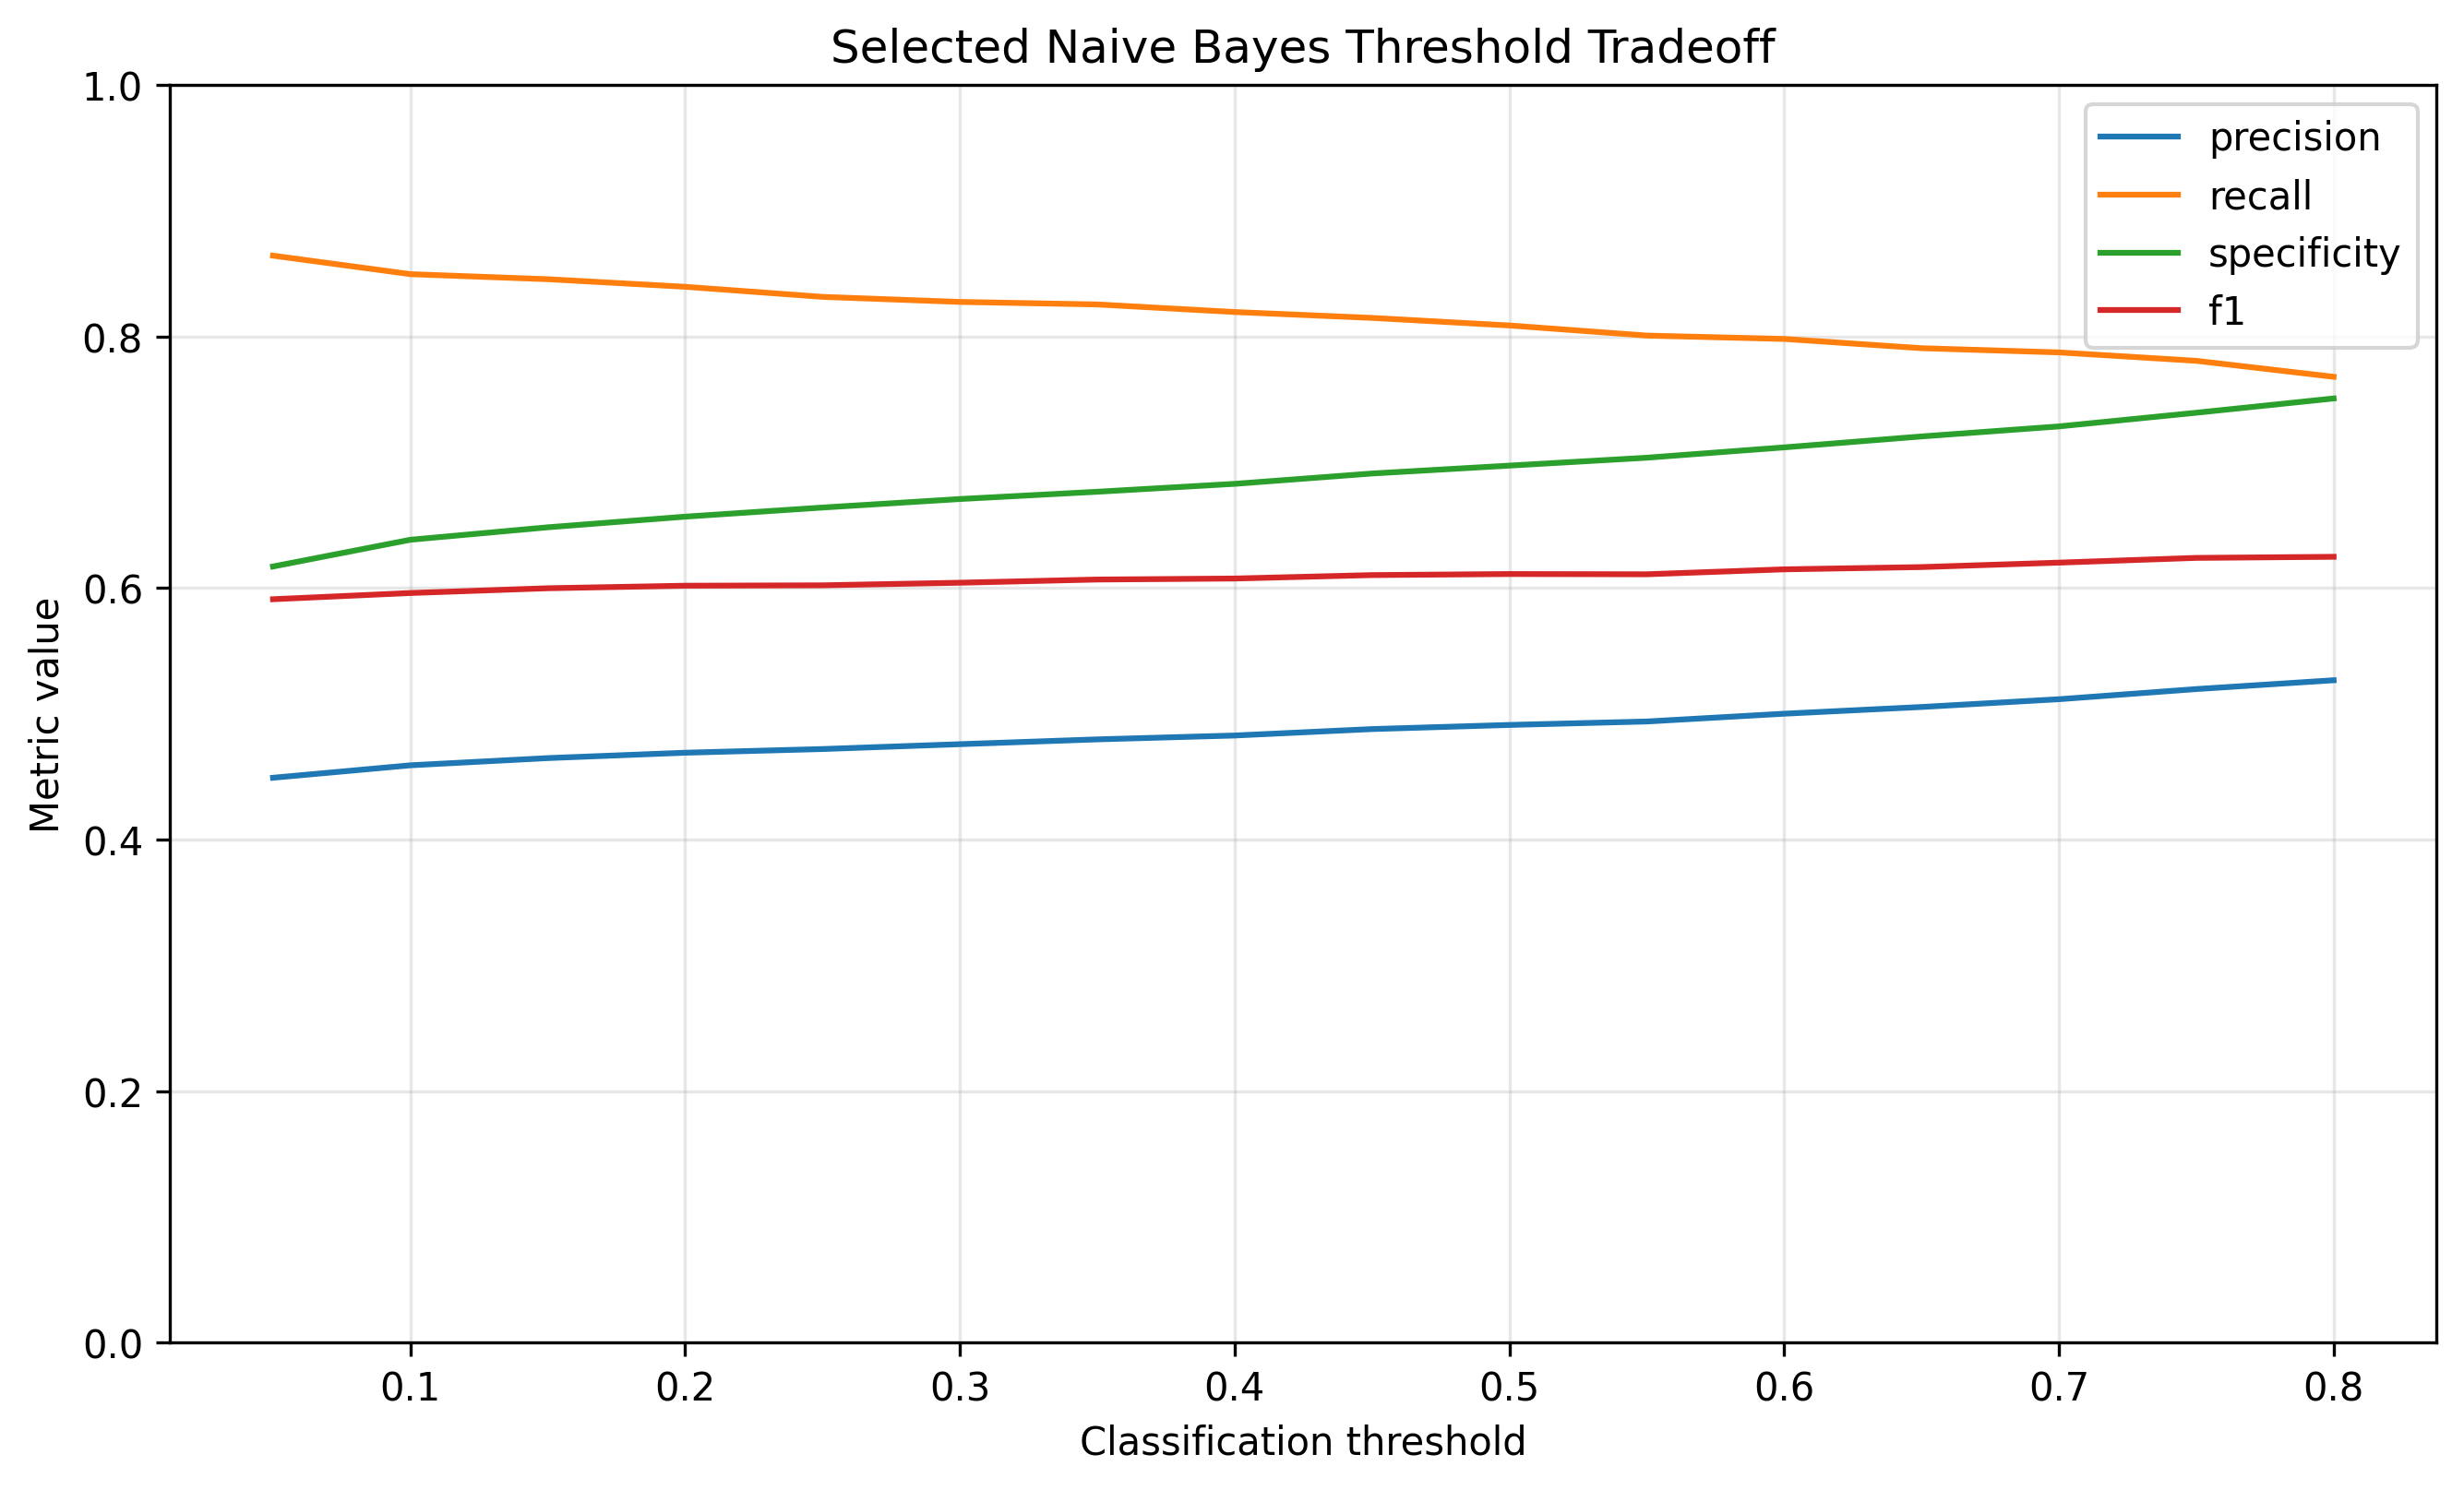
\includegraphics[width=0.88\textwidth]{../figures/naive_bayes_threshold_tradeoff.png}
\caption{Threshold tradeoff for the selected Naive Bayes model}
\label{fig:nb-threshold-tradeoff}
\end{figure}

At threshold \(0.50\), the selected model has precision approximately \(0.462\), recall approximately \(0.847\), specificity approximately \(0.644\), and \(F_1\) approximately \(0.598\). At threshold \(0.95\), recall is still approximately \(0.813\), while precision only rises to approximately \(0.492\). This indicates that many predicted probabilities are pushed toward high values. Such overconfident probabilities are consistent with the Naive Bayes independence assumption being violated by correlated feature groups.

This does not mean that the model is useless. It ranks customers much better than chance. However, it suggests that Naive Bayes probability levels should not be interpreted as calibrated churn probabilities without further calibration analysis.

\subsection{ROC and precision-recall curves}

Figure~\ref{fig:nb-roc-curve} shows the ROC curve for the selected Naive Bayes model. The ROC-AUC is approximately \(0.819\), clearly above the random-ranking line. This confirms that Naive Bayes learns meaningful churn-discriminating structure.

\begin{figure}[H]
\centering
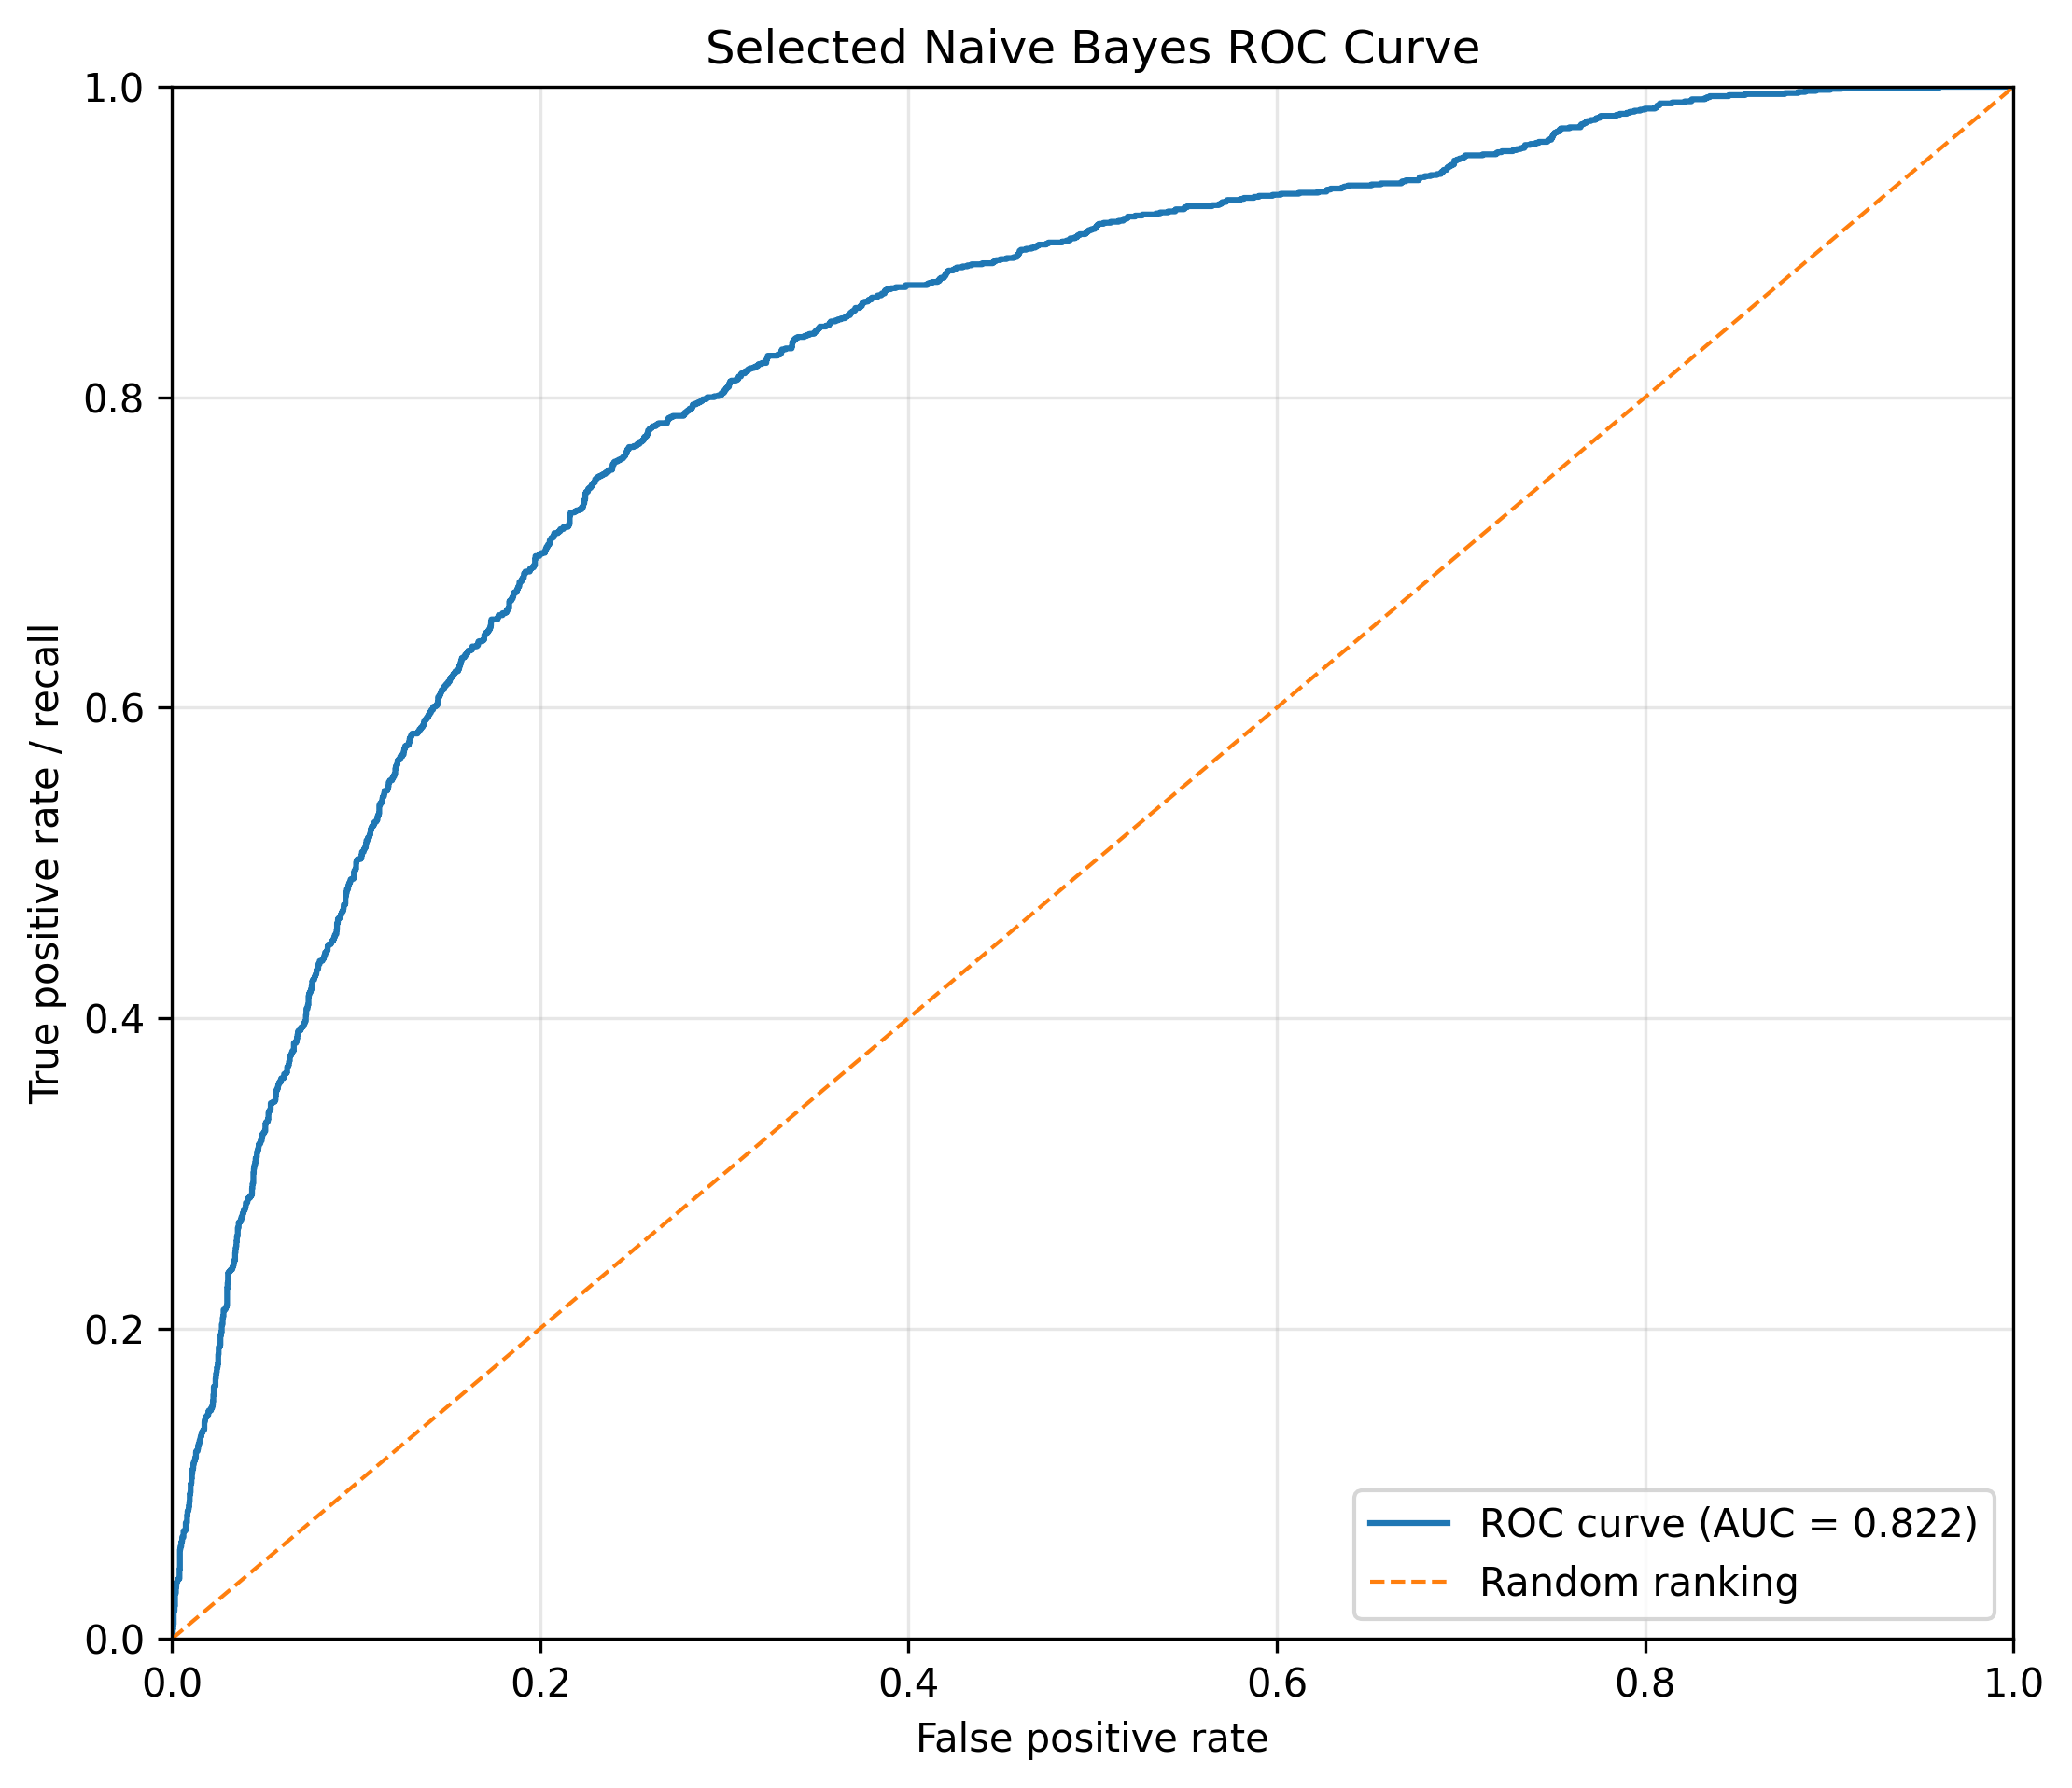
\includegraphics[width=0.72\textwidth]{../figures/naive_bayes_roc_curve.png}
\caption{ROC curve for the selected Naive Bayes model}
\label{fig:nb-roc-curve}
\end{figure}

Figure~\ref{fig:nb-pr-curve} shows the precision-recall curve. The PR-AUC is approximately \(0.604\), well above the positive-rate baseline of approximately \(0.265\). This indicates useful positive-class retrieval ability. However, the PR-AUC remains lower than the corresponding logistic regression and kNN values, so Naive Bayes is not the strongest ranking model so far.

\begin{figure}[H]
\centering
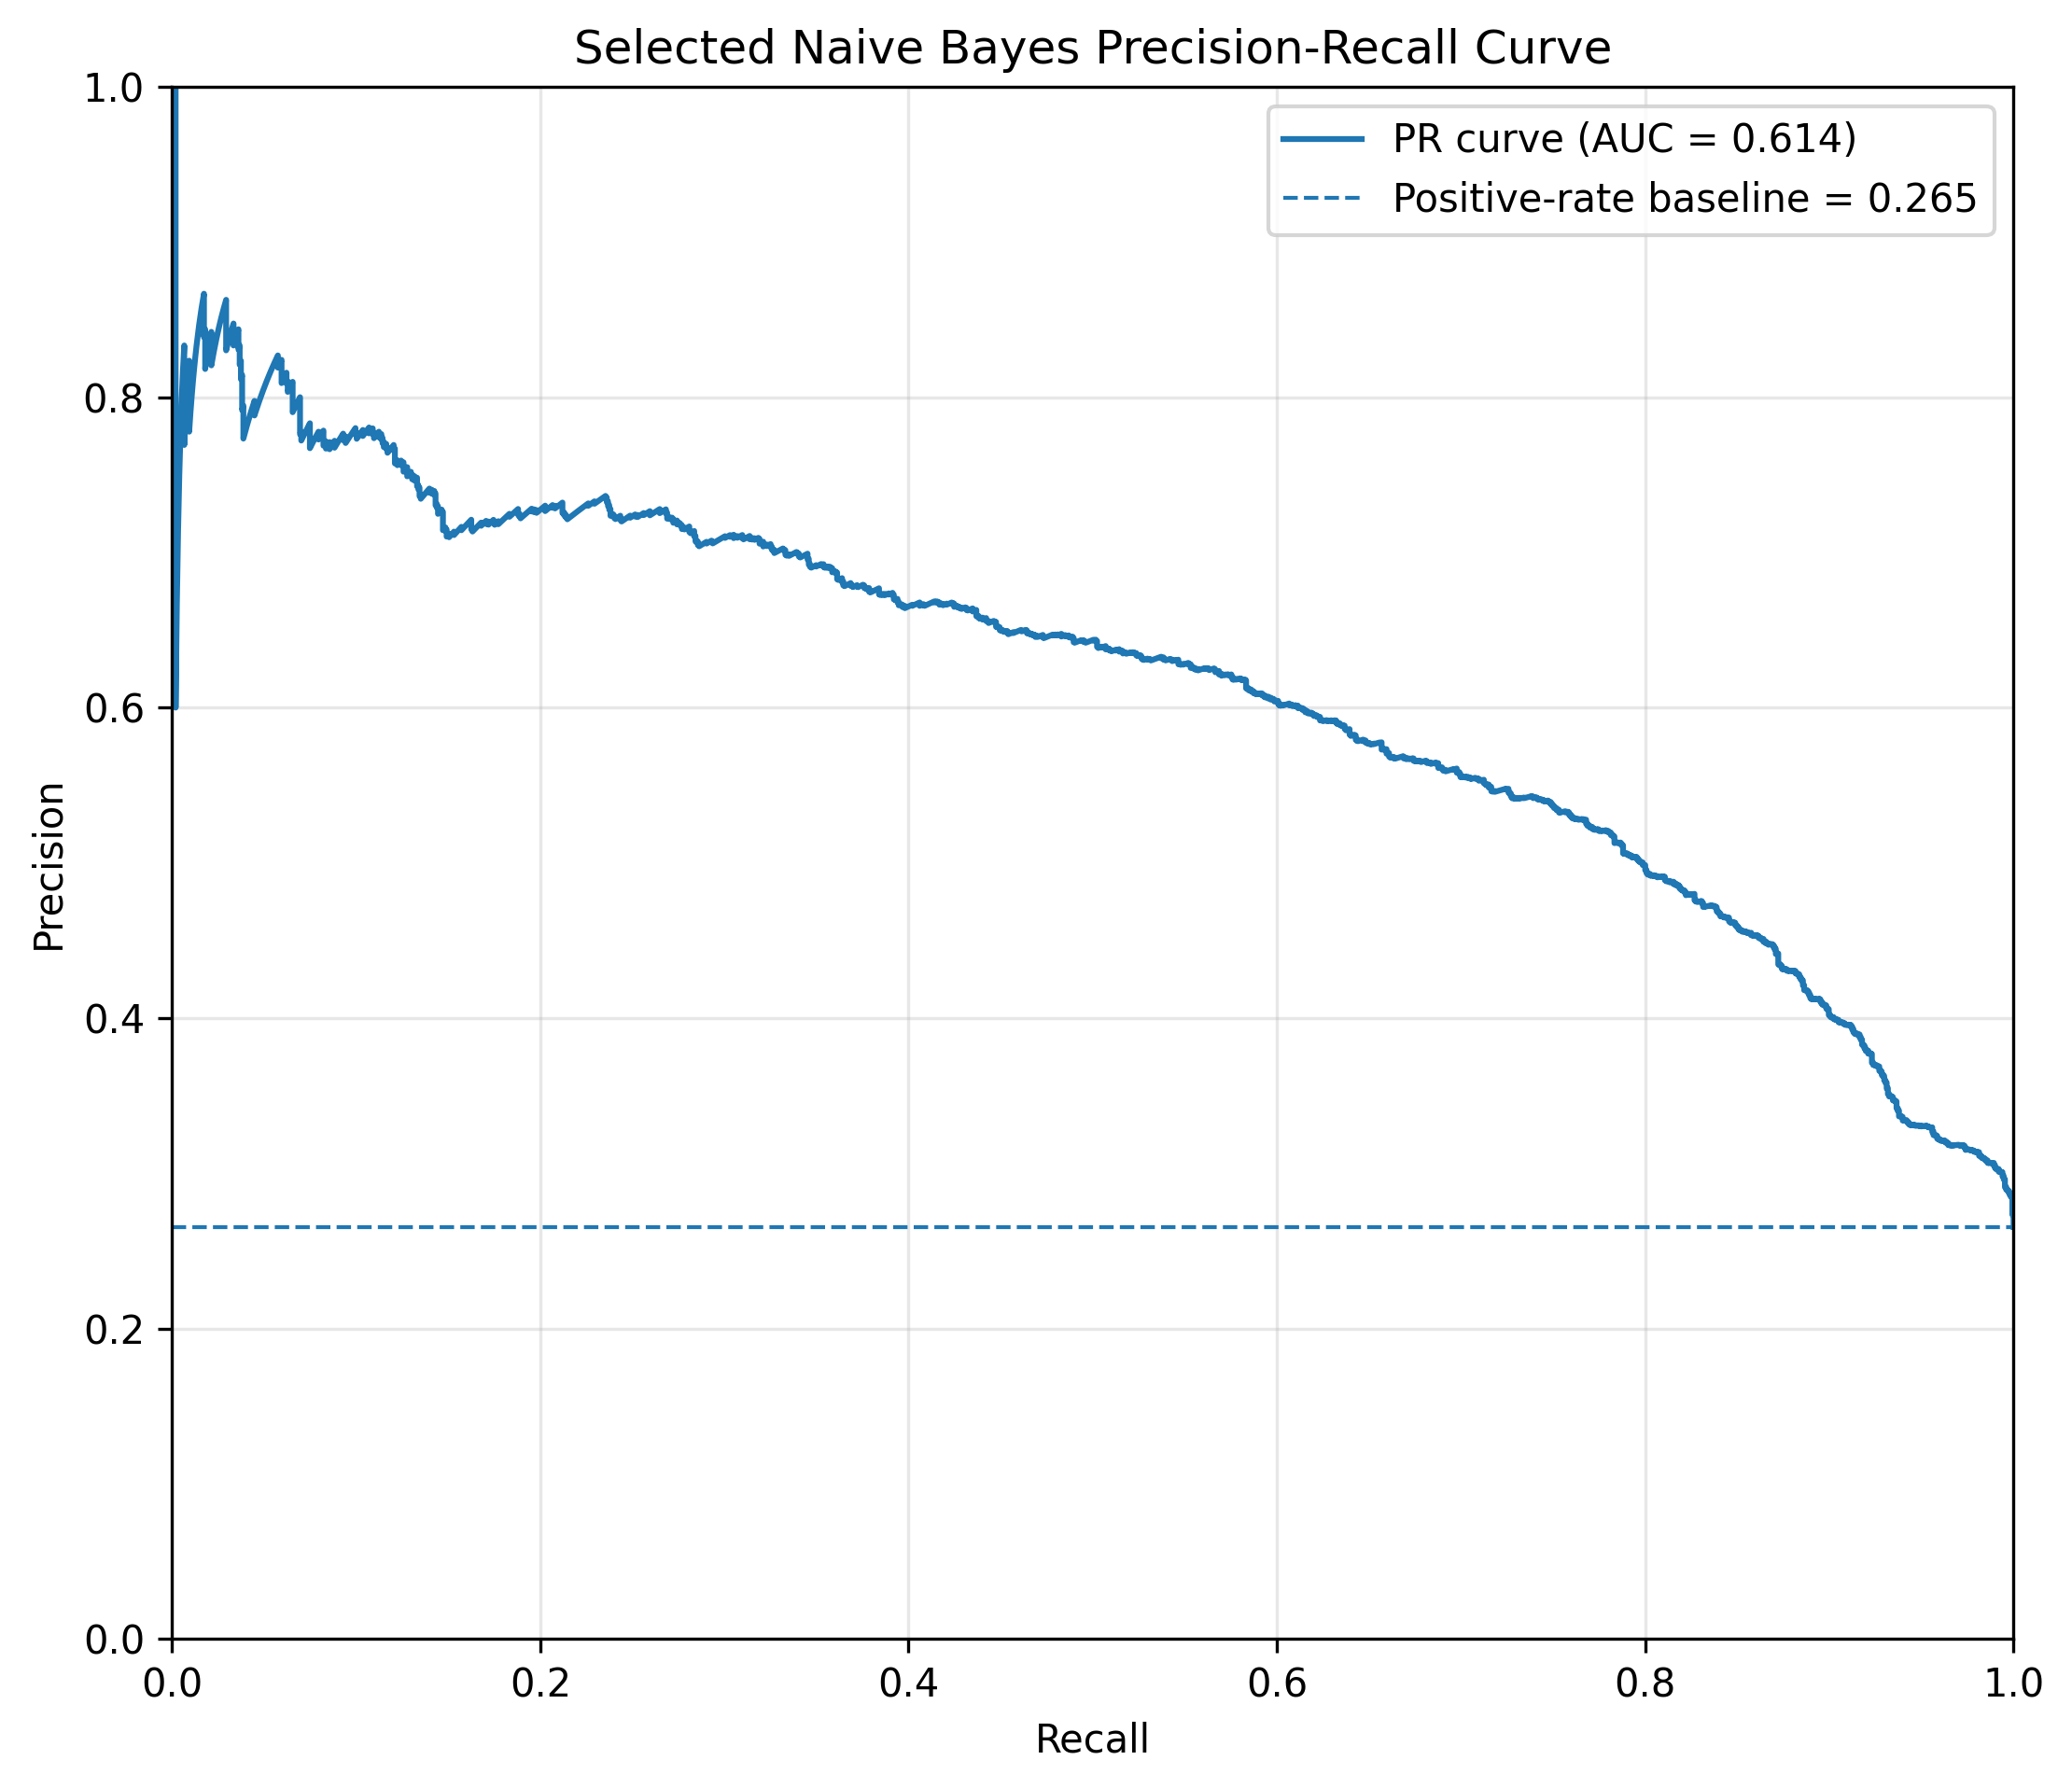
\includegraphics[width=0.72\textwidth]{../figures/naive_bayes_precision_recall_curve.png}
\caption{Precision-recall curve for the selected Naive Bayes model}
\label{fig:nb-pr-curve}
\end{figure}

\subsection{Summary}

The Naive Bayes experiment shows that a simple generative model can capture meaningful churn patterns. The selected full transformed Gaussian Naive Bayes model has high recall and useful ROC-AUC and PR-AUC. It is especially good at detecting many churners, but it does so by flagging a large fraction of the customer base.

The main limitation is probability behaviour. Because many Telco features are correlated, the conditional-independence assumption is not realistic. This likely causes related evidence to be counted multiple times and produces overconfident predicted probabilities. The threshold curve reflects this: increasing the threshold does not reduce recall as sharply as expected, and precision remains relatively low.

Compared with the learned models evaluated so far, Naive Bayes is useful but not dominant. Logistic regression remains the strongest model family so far by PR-AUC and ROC-AUC, while kNN is also stronger than Naive Bayes on these ranking metrics. Nevertheless, Naive Bayes adds an important modelling perspective: it connects classification to Bayes' rule, class priors, class-conditional likelihoods, smoothing, and the difference between ideal Bayes classification and practical approximate generative modelling.


\newpage
\newpage
\section{Decision Trees}
\label{sec:decision-trees}

This section evaluates single decision-tree classifiers for churn prediction. Decision trees are useful at this stage because they introduce nonlinear, rule-based classification without yet using ensembles. A fitted tree partitions the transformed feature space into regions, assigns each region a local churn proportion, and uses that local proportion both for hard classification and for ranking customers by churn risk.

The same development discipline is used as in the previous modelling sections. The held-out test set is not used. All reported results are based on stratified cross-validation inside the training set, using out-of-fold predictions where possible. The comparisons in this section are therefore development-stage comparisons of decision-tree variants. They identify a representative single-tree candidate within the tried configurations, but they are not final test-set performance claims.

\subsection{Recursive partitioning}

Let the training data be
\[
\mathcal{D}_{\mathrm{train}}
=
\{(x_i,y_i)\}_{i=1}^{n},
\]
where \(x_i\) is the transformed customer feature vector and \(y_i\in\{0,1\}\) is the churn label. A decision tree recursively splits the feature space into smaller regions. Each internal node applies a rule of the form
\[
x_j \leq s,
\]
where \(x_j\) is one feature and \(s\) is a split value. For one-hot encoded categorical indicators, these split rules often test whether a category indicator is zero or one.

After the recursive splitting process, each terminal node or leaf contains a subset of training observations. For a leaf \(R_m\), the estimated churn probability is the local class proportion:
\[
\widehat{p}_m
=
\frac{1}{|R_m|}
\sum_{i:x_i\in R_m} y_i.
\]
For a new customer \(x\), the fitted tree sends \(x\) to one leaf and predicts
\[
\widehat{p}(Y=1\mid X=x)=\widehat{p}_m.
\]
The default hard prediction at threshold \(0.5\) is
\[
\widehat{y}
=
\mathbb{1}\{\widehat{p}(Y=1\mid X=x)\geq 0.5\}.
\]
Thus, a classification tree can be interpreted as a collection of local empirical churn-rate rules.

\subsection{Split selection and impurity}

Tree construction is greedy. At a node, the algorithm evaluates candidate feature-threshold splits and chooses the split that most improves class purity. It does not search globally over all possible trees, because the number of possible tree structures is too large.

For binary classification, one common impurity measure is the Gini impurity. If a node has churn proportion \(p\), its Gini impurity is
\[
G(p)
=
1-p^2-(1-p)^2
=
2p(1-p).
\]
The impurity is zero when the node is pure, meaning \(p=0\) or \(p=1\). It is largest when the node is evenly mixed, meaning \(p=0.5\).

For a candidate split that divides a parent node \(R\) into left and right children \(R_L\) and \(R_R\), the weighted child impurity is
\[
G_{\mathrm{children}}
=
\frac{|R_L|}{|R|}G(R_L)
+
\frac{|R_R|}{|R|}G(R_R).
\]
The split improvement is
\[
\Delta G
=
G(R)-G_{\mathrm{children}}.
\]
The greedy algorithm chooses the candidate split with the largest impurity reduction. Entropy and information gain follow the same logic, but use
\[
H(p)
=
-p\log(p)-(1-p)\log(1-p)
\]
instead of Gini impurity.

\subsection{Ranking with decision trees}

Although decision trees are often described as rule-based classifiers, they also produce scores. The score for a customer is the estimated churn proportion in the leaf that the customer reaches. Therefore, decision trees rank customers by leaf churn rate.

This ranking has a specific structure. All customers in the same leaf receive exactly the same score, so the ranking is stepwise and can contain many ties. A shallow or strongly pruned tree has fewer leaves and therefore fewer possible score levels. This makes its ranking coarse but often more stable. A deeper tree has more leaves and more possible score levels, but the estimated leaf probabilities can be noisy when leaves contain few observations.

This matters for ROC-AUC and precision-recall analysis. Trees are trained by local impurity reduction, not by directly optimizing ROC-AUC or PR-AUC. Ranking quality must therefore be evaluated explicitly from out-of-fold predicted probabilities.

\subsection{Regularization and pruning}

Unrestricted decision trees can overfit. A deep tree can keep splitting until leaves become very small, fitting local noise and idiosyncratic training patterns. This lowers training impurity but can harm validation performance.

This section evaluates two forms of tree regularization. The first is pre-pruning, where tree growth is restricted during fitting through hyperparameters such as
\[
\texttt{max\_depth},\qquad
\texttt{min\_samples\_split},\qquad
\texttt{min\_samples\_leaf}.
\]
The second is cost-complexity pruning, controlled in scikit-learn by \(\texttt{ccp\_alpha}\). Cost-complexity pruning grows a large tree and then selects a smaller subtree by penalizing complexity. Conceptually, the pruning criterion has the form
\[
\text{training impurity}
+
\alpha \times \text{tree complexity},
\]
where larger \(\alpha\) favours smaller trees.

The pruning parameter is a hyperparameter like \(\texttt{max\_depth}\) or \(\texttt{min\_samples\_leaf}\). In this section it is selected with cross-validation inside the training set. This is appropriate for development-stage model selection. However, if a separate validation set were reserved for higher-level model-family comparison, that same validation set should not also be used to choose the pruning level. A stricter estimate of the full tune-and-select procedure would require nested validation. This section does not claim to provide such a final unbiased estimate; final testing remains deferred.

\subsection{Experimental design}

Four decision-tree variants are evaluated:

\begin{itemize}[leftmargin=*]
    \item \textbf{Decision stump}: a depth-one tree.
    \item \textbf{Default decision tree}: an unrestricted baseline tree.
    \item \textbf{Pre-pruned tree grid}: a grid over \(\texttt{criterion}\), \(\texttt{max\_depth}\), \(\texttt{min\_samples\_split}\), and \(\texttt{min\_samples\_leaf}\).
    \item \textbf{Cost-complexity-pruned tree grid}: a grid over candidate \(\texttt{ccp\_alpha}\) values.
\end{itemize}

The representative decision tree is selected by cross-validated PR-AUC, with balanced accuracy and \(F_1\) used as secondary criteria. PR-AUC remains the primary criterion because churn is the minority class and positive-class retrieval is central to the project.

\subsection{Pre-pruning results}

Figure~\ref{fig:decision-tree-prepruned-pr-auc} shows the pre-pruning grid from the perspective of PR-AUC. Very shallow trees underfit the ranking problem, while moderately deep trees perform better. The best PR-AUC occurs at depth 6 with \(\texttt{min\_samples\_leaf}=10\). The unrestricted-depth setting performs worse, especially when \(\texttt{min\_samples\_leaf}=1\), which is consistent with overfitting.

\begin{figure}[H]
\centering
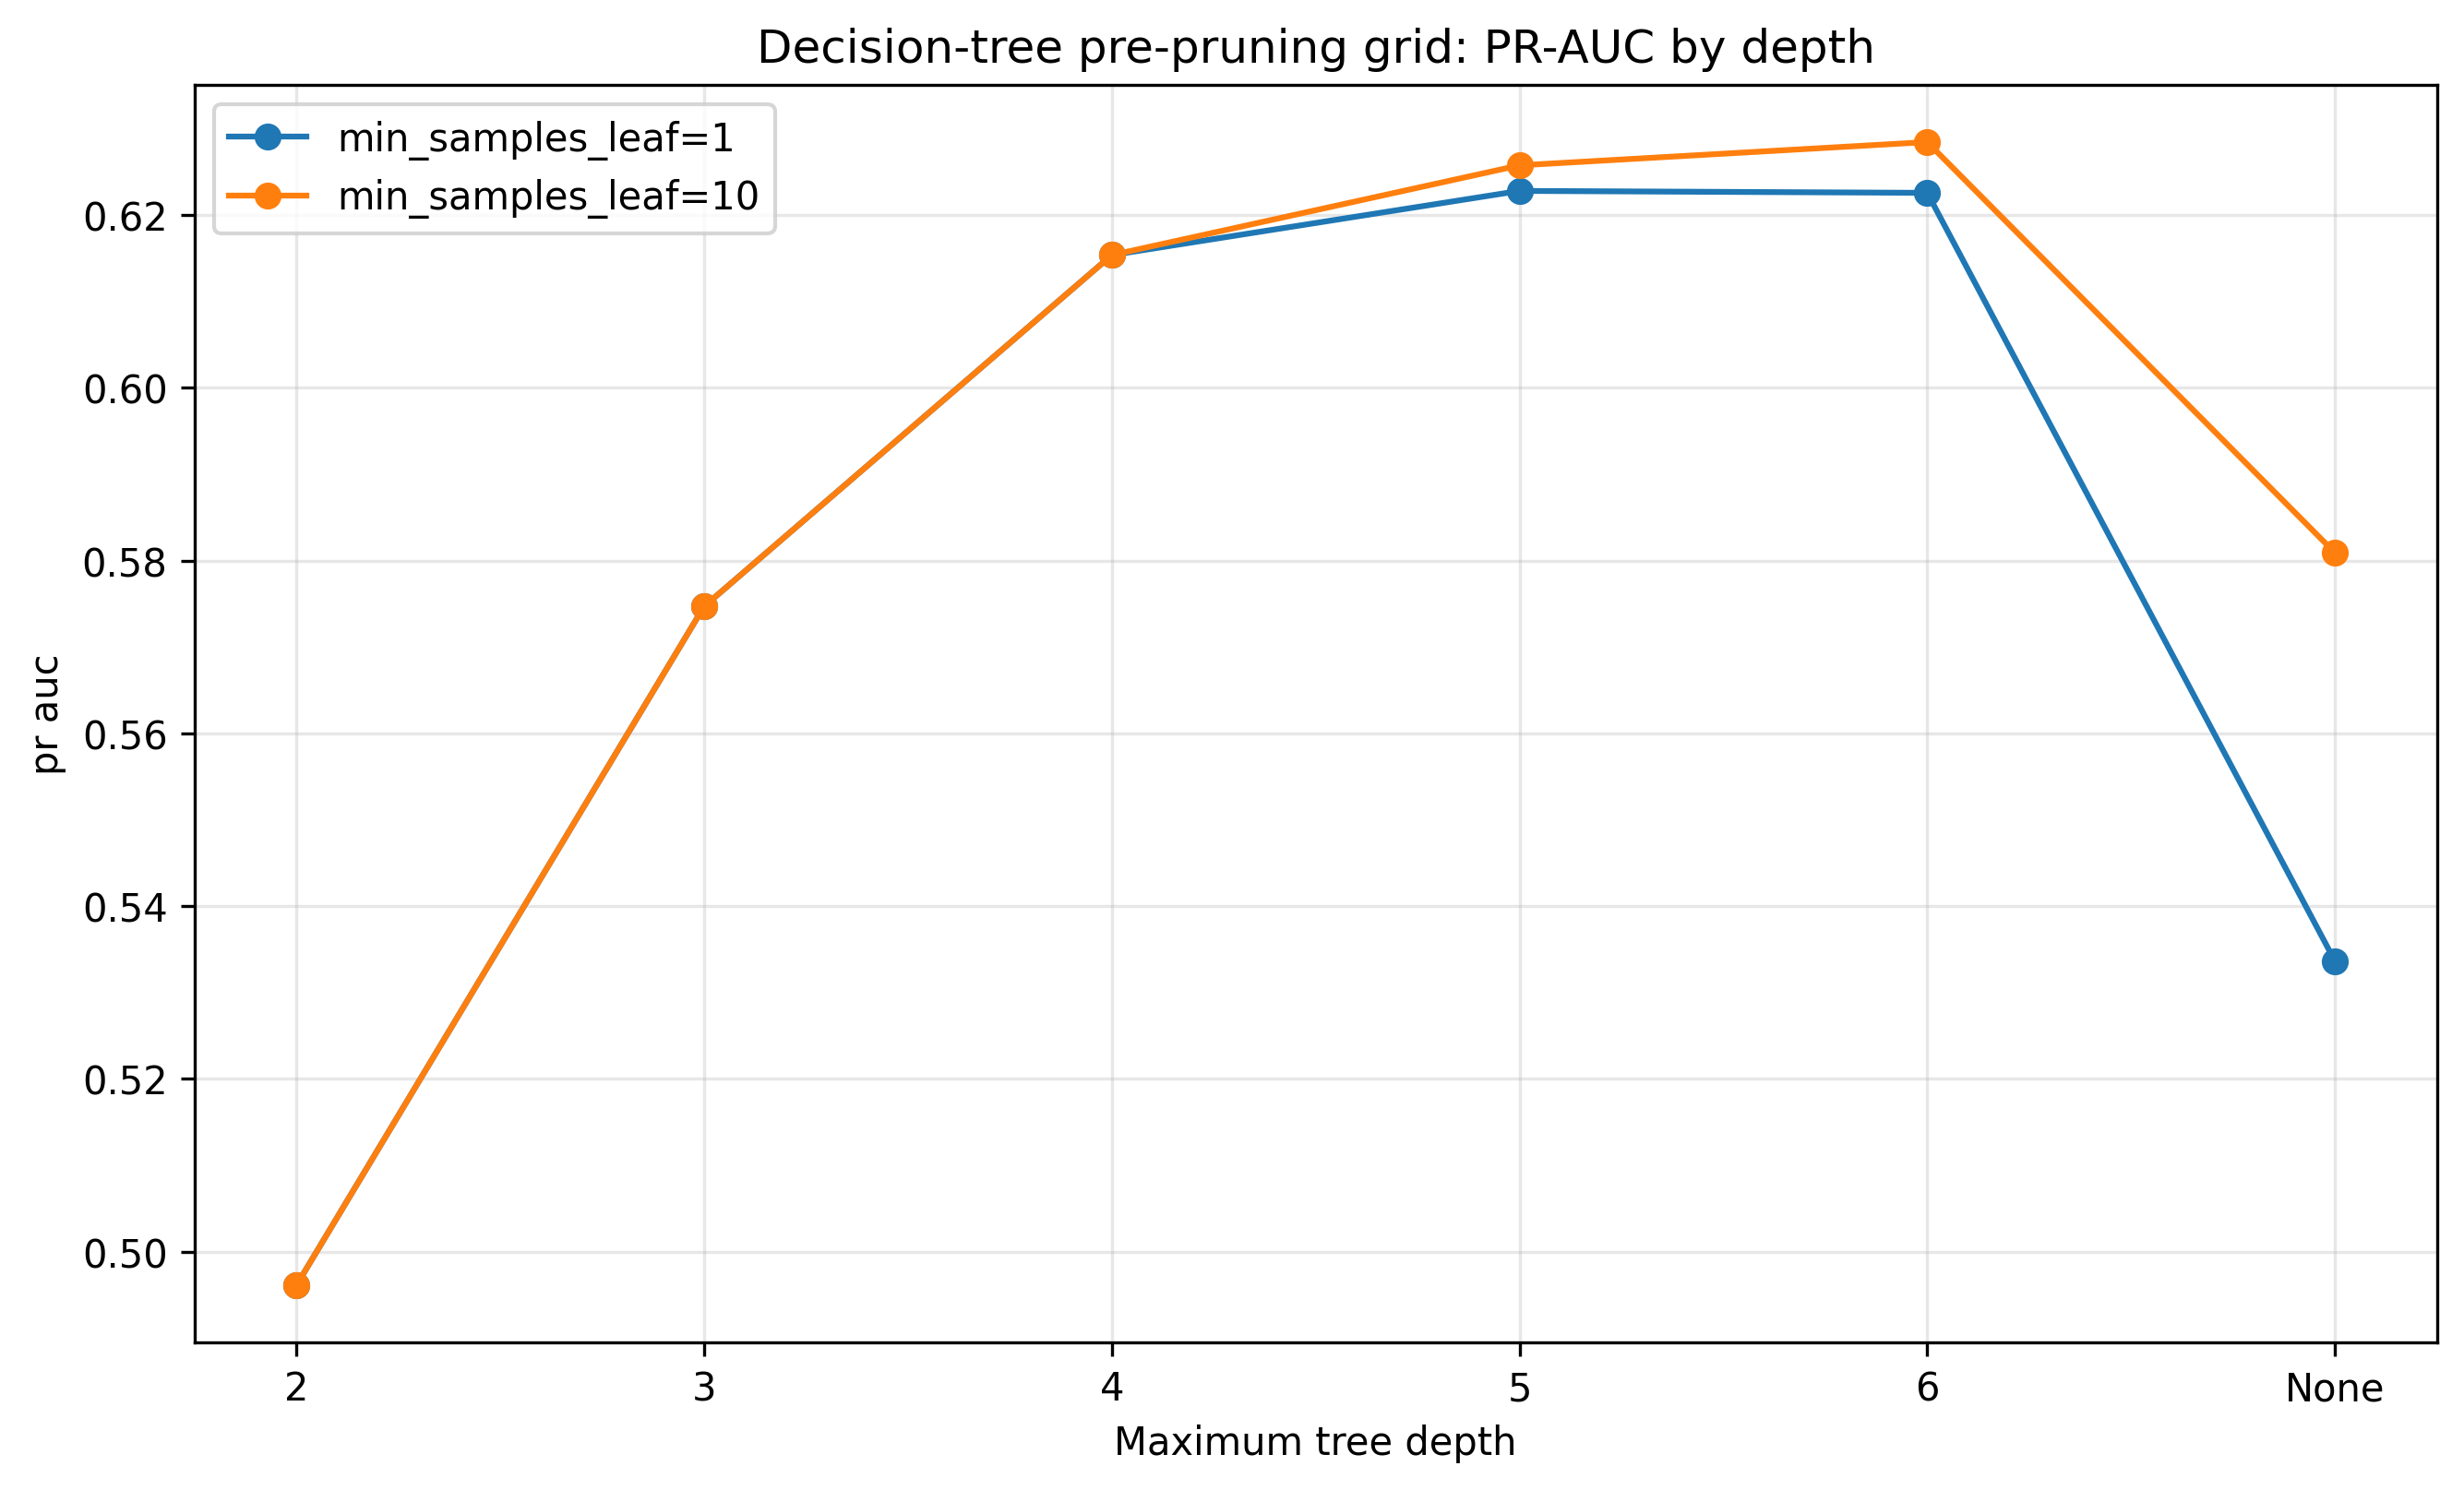
\includegraphics[width=0.88\textwidth]{../figures/decision_tree_prepruned_pr_auc_by_depth.png}
\caption{Decision-tree pre-pruning grid: PR-AUC by maximum depth}
\label{fig:decision-tree-prepruned-pr-auc}
\end{figure}

Figure~\ref{fig:decision-tree-prepruned-balanced-accuracy} shows the same grid using balanced accuracy. The depth-two tree has high balanced accuracy but weak PR-AUC, showing that a good default-threshold class split is not the same as strong ranking performance. The depth-five and depth-six trees provide stronger ranking performance while keeping the tree sufficiently regularized.

\begin{figure}[H]
\centering
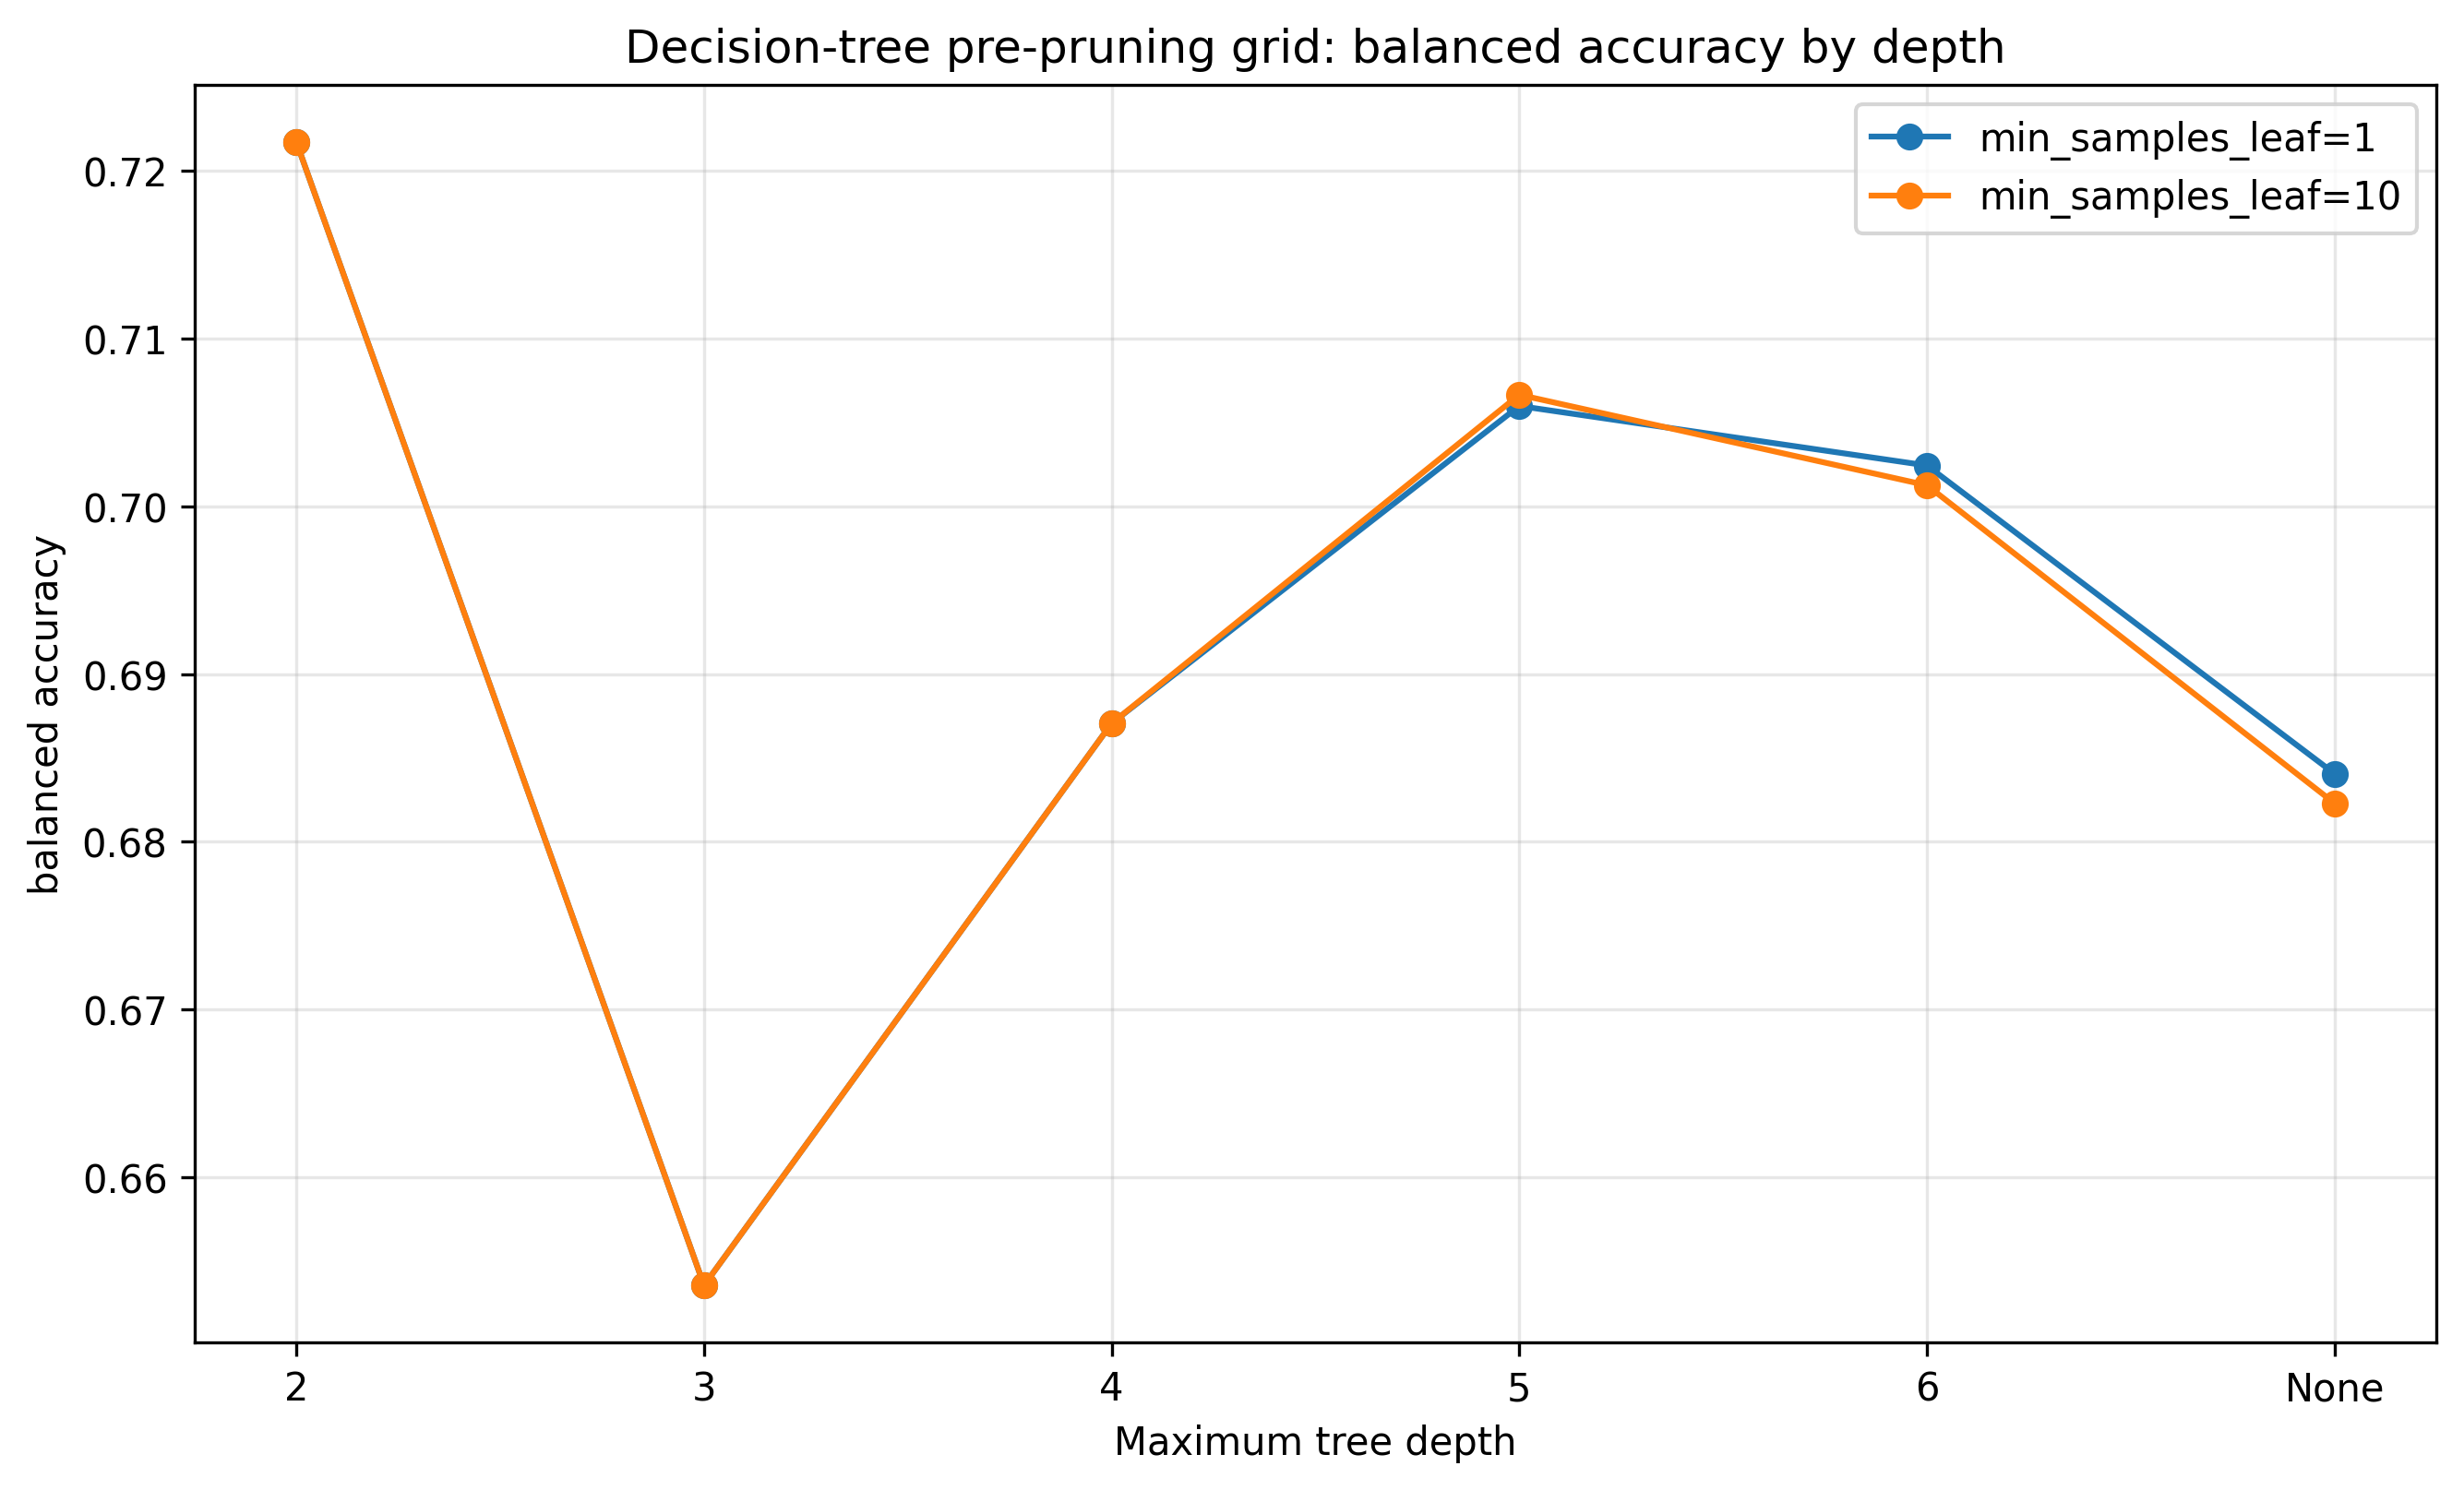
\includegraphics[width=0.88\textwidth]{../figures/decision_tree_prepruned_balanced_accuracy_by_depth.png}
\caption{Decision-tree pre-pruning grid: balanced accuracy by maximum depth}
\label{fig:decision-tree-prepruned-balanced-accuracy}
\end{figure}

\subsection{Cost-complexity pruning results}

Figure~\ref{fig:decision-tree-ccp-alpha} shows the cost-complexity pruning grid. The unpruned tree has weak PR-AUC because it overfits. As \(\texttt{ccp\_alpha}\) increases, the tree becomes smaller and the ranking metrics improve substantially. The best cost-complexity-pruned tree reaches PR-AUC approximately \(0.615\), which is much better than the default unrestricted tree but still below the best pre-pruned tree.

\begin{figure}[H]
\centering
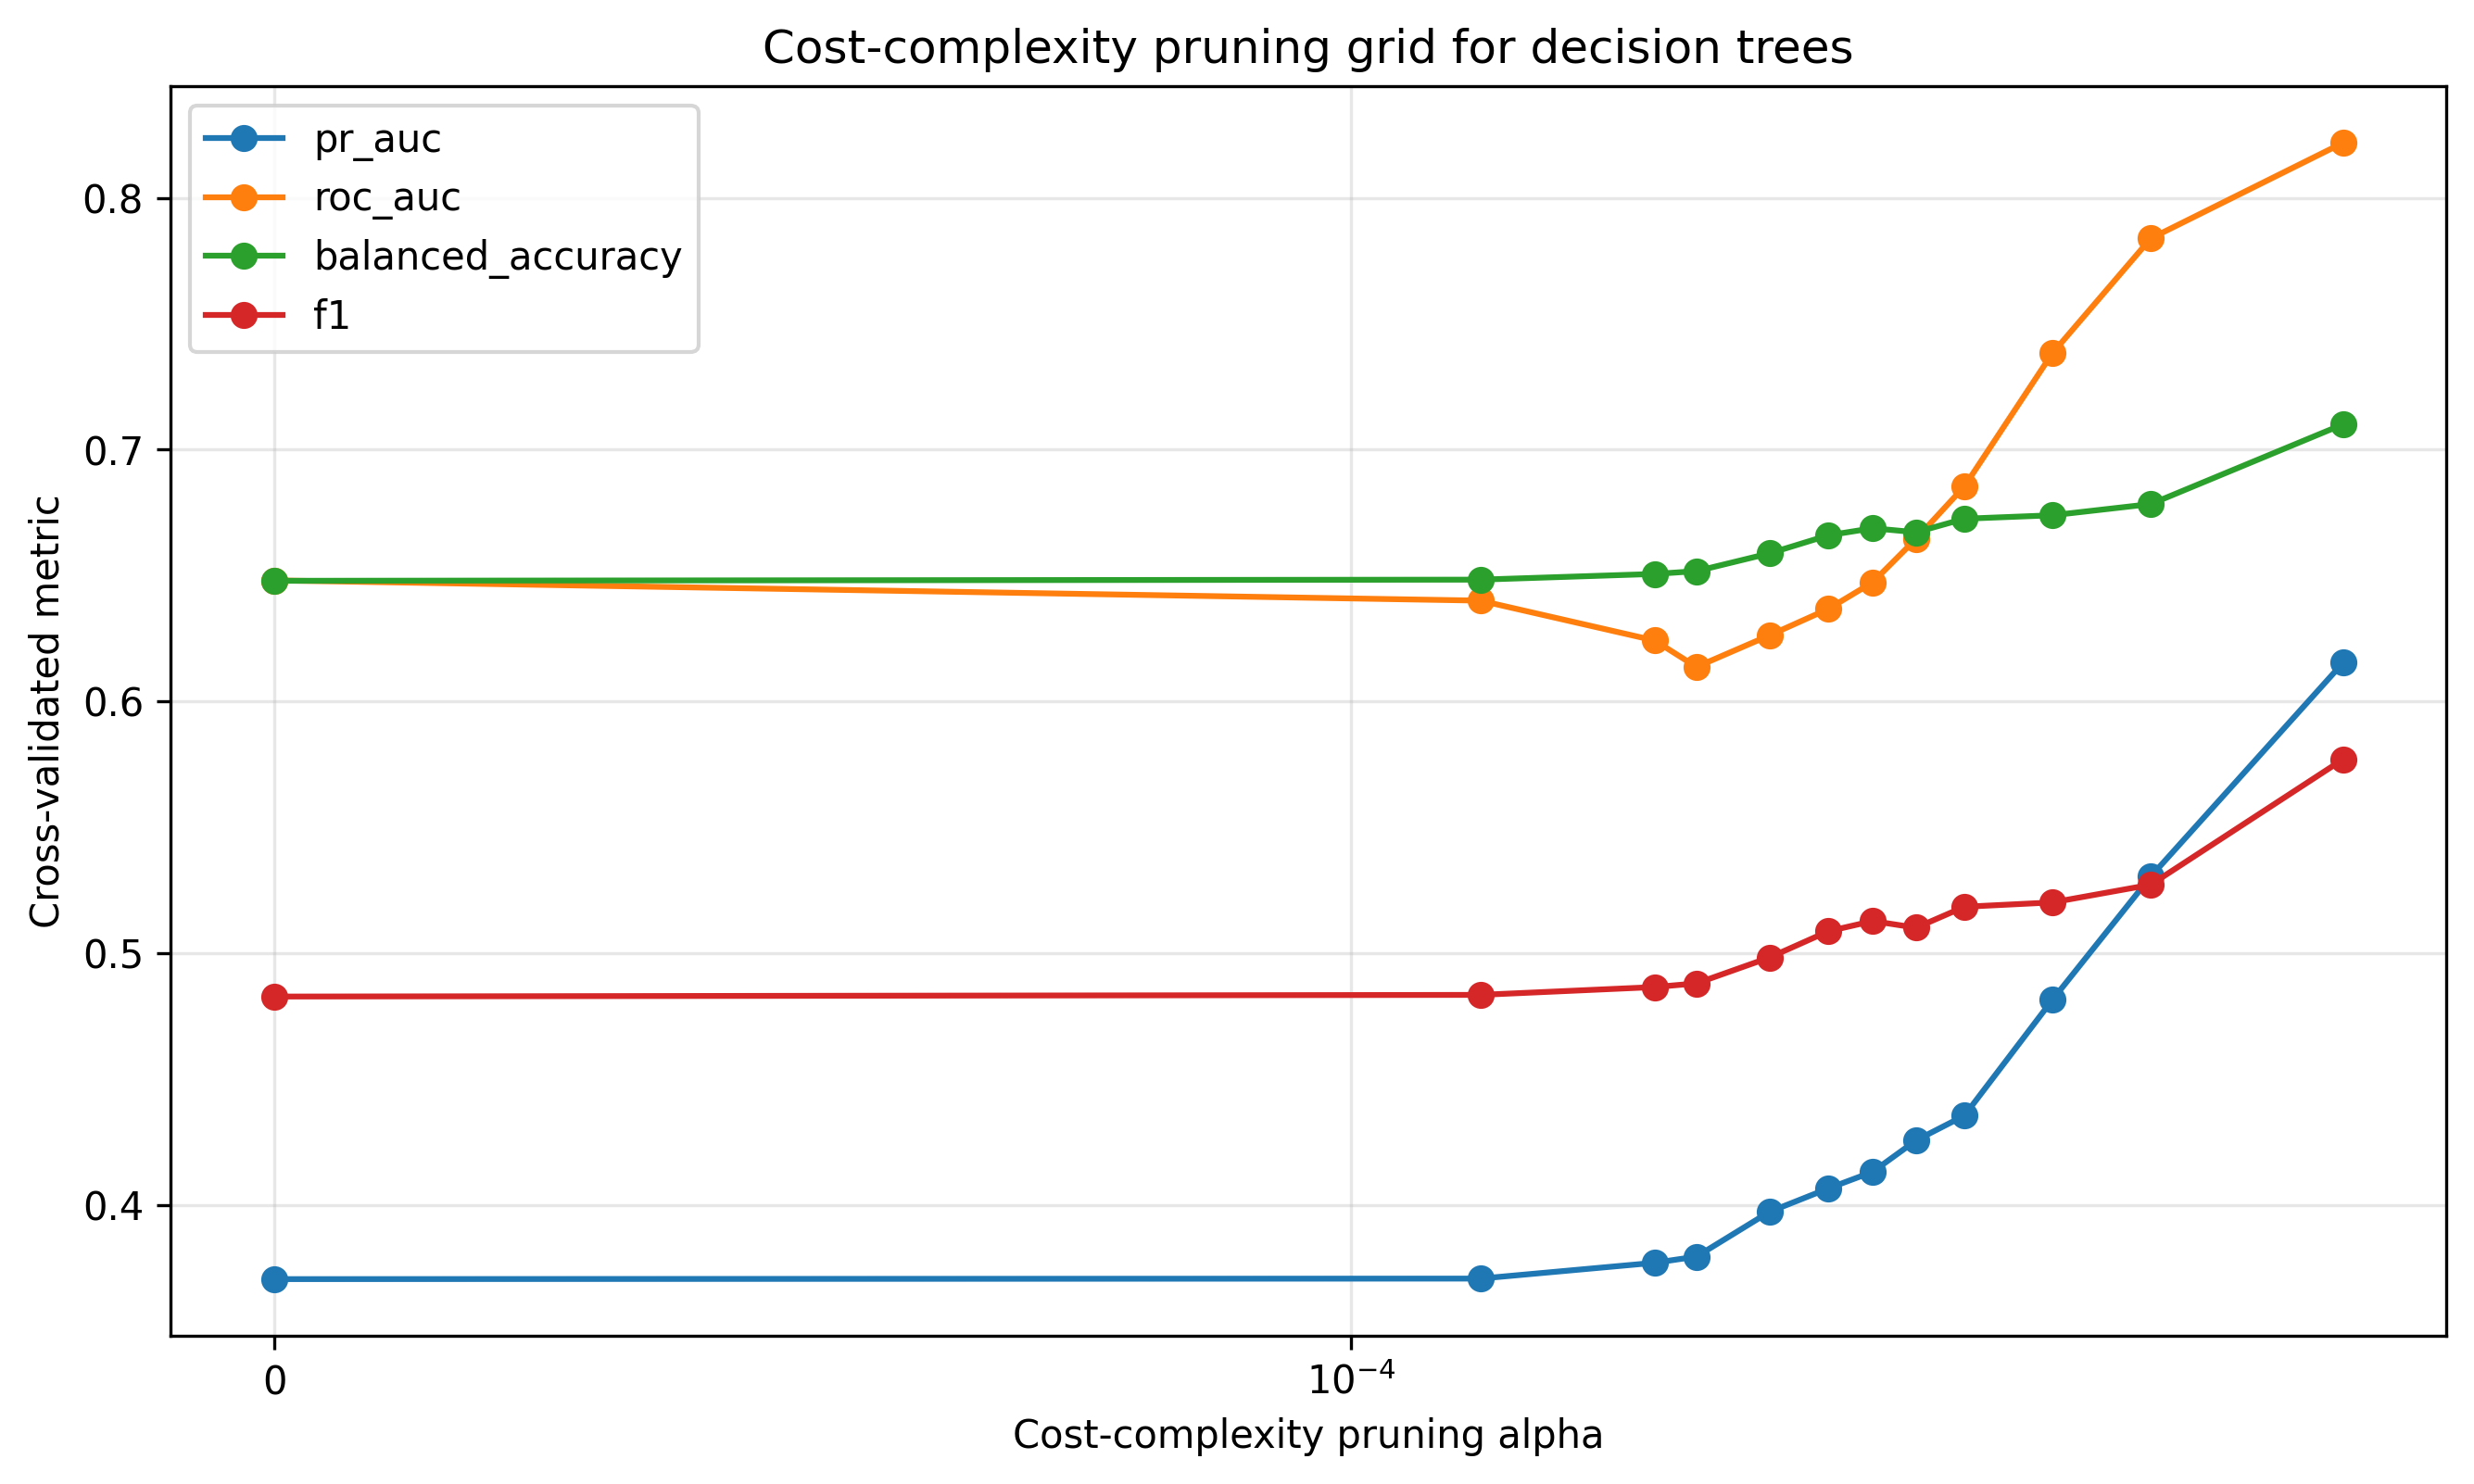
\includegraphics[width=0.88\textwidth]{../figures/decision_tree_ccp_alpha_metrics.png}
\caption{Cost-complexity pruning metrics for decision trees}
\label{fig:decision-tree-ccp-alpha}
\end{figure}

The pruning result is useful because it demonstrates the central decision-tree bias-variance tradeoff. A larger tree can fit training irregularities, but a smaller pruned tree can generalize better. In this dataset, however, direct pre-pruning with a moderate maximum depth and minimum leaf size gives the strongest single-tree ranking result.

\subsection{Model comparison}

Table~\ref{tab:decision-tree-model-comparison} compares the main decision-tree variants. The selected model is a Gini tree with \(\texttt{max\_depth}=6\), \(\texttt{min\_samples\_split}=25\), \(\texttt{min\_samples\_leaf}=10\), and \(\texttt{ccp\_alpha}=0\). It has PR-AUC approximately \(0.628\) and ROC-AUC approximately \(0.824\). It improves sharply over the default unrestricted tree, whose PR-AUC is only approximately \(0.371\).

\begin{table}[H]
\centering
\small
\resizebox{\textwidth}{!}{
\begin{tabular}{lrrrrrrrr}
\toprule
Model & Accuracy & Bal. Acc. & Precision & Recall & Specificity & \(F_1\) & ROC-AUC & PR-AUC \\
\midrule
Selected pre-pruned tree & 0.789 & 0.701 & 0.624 & 0.514 & 0.888 & 0.564 & 0.824 & 0.628 \\
Best cost-complexity-pruned tree & 0.790 & 0.710 & 0.620 & 0.540 & 0.880 & 0.577 & 0.822 & 0.615 \\
Decision stump & 0.735 & 0.500 & 0.000 & 0.000 & 1.000 & 0.000 & 0.726 & 0.413 \\
Default unrestricted tree & 0.725 & 0.648 & 0.482 & 0.484 & 0.812 & 0.483 & 0.648 & 0.371 \\
\bottomrule
\end{tabular}
}
\caption{Cross-validated decision-tree model comparison on the training set}
\label{tab:decision-tree-model-comparison}
\end{table}

The corresponding positive-first confusion-matrix counts are shown in Table~\ref{tab:decision-tree-confusion}. At the default threshold, the selected pre-pruned tree detects \(769\) of the \(1495\) churners and misses \(726\). It flags \(463\) non-churners as churn risks and correctly classifies \(3676\) non-churners.

\begin{table}[H]
\centering
\small
\begin{tabular}{lrrrr}
\toprule
Model & TP & FN & FP & TN \\
\midrule
Selected pre-pruned tree & 769 & 726 & 463 & 3676 \\
Best cost-complexity-pruned tree & 807 & 688 & 495 & 3644 \\
Decision stump & 0 & 1495 & 0 & 4139 \\
Default unrestricted tree & 723 & 772 & 777 & 3362 \\
\bottomrule
\end{tabular}
\caption{Positive-first confusion-matrix counts for decision-tree models}
\label{tab:decision-tree-confusion}
\end{table}

The decision stump has ordinary accuracy equal to the no-churn majority baseline and predicts no churn at the default threshold. Nevertheless, its ROC-AUC is above \(0.7\), because the stump still assigns different leaf probabilities and therefore contains some ranking information. This illustrates why hard classification metrics and ranking metrics answer different questions.

Compared with previous model families, the selected tree is useful but not dominant. It is much better than the default unrestricted tree and stronger than Naive Bayes by PR-AUC, but it remains below logistic regression from Section~\ref{sec:linear-classification-and-logistic-regression}. Its PR-AUC is close to selected k-nearest neighbours from Section~\ref{sec:knn}. This supports continuing to tree ensembles later: a single tree captures meaningful nonlinear churn structure, but its instability and coarse leaf-based scoring limit its standalone performance.

\subsection{Threshold behaviour}

Figure~\ref{fig:decision-tree-threshold-tradeoff} shows the threshold tradeoff for the selected tree. Lower thresholds increase recall but also create many more false positives. Higher thresholds improve precision and specificity, but recall falls.

\begin{figure}[H]
\centering
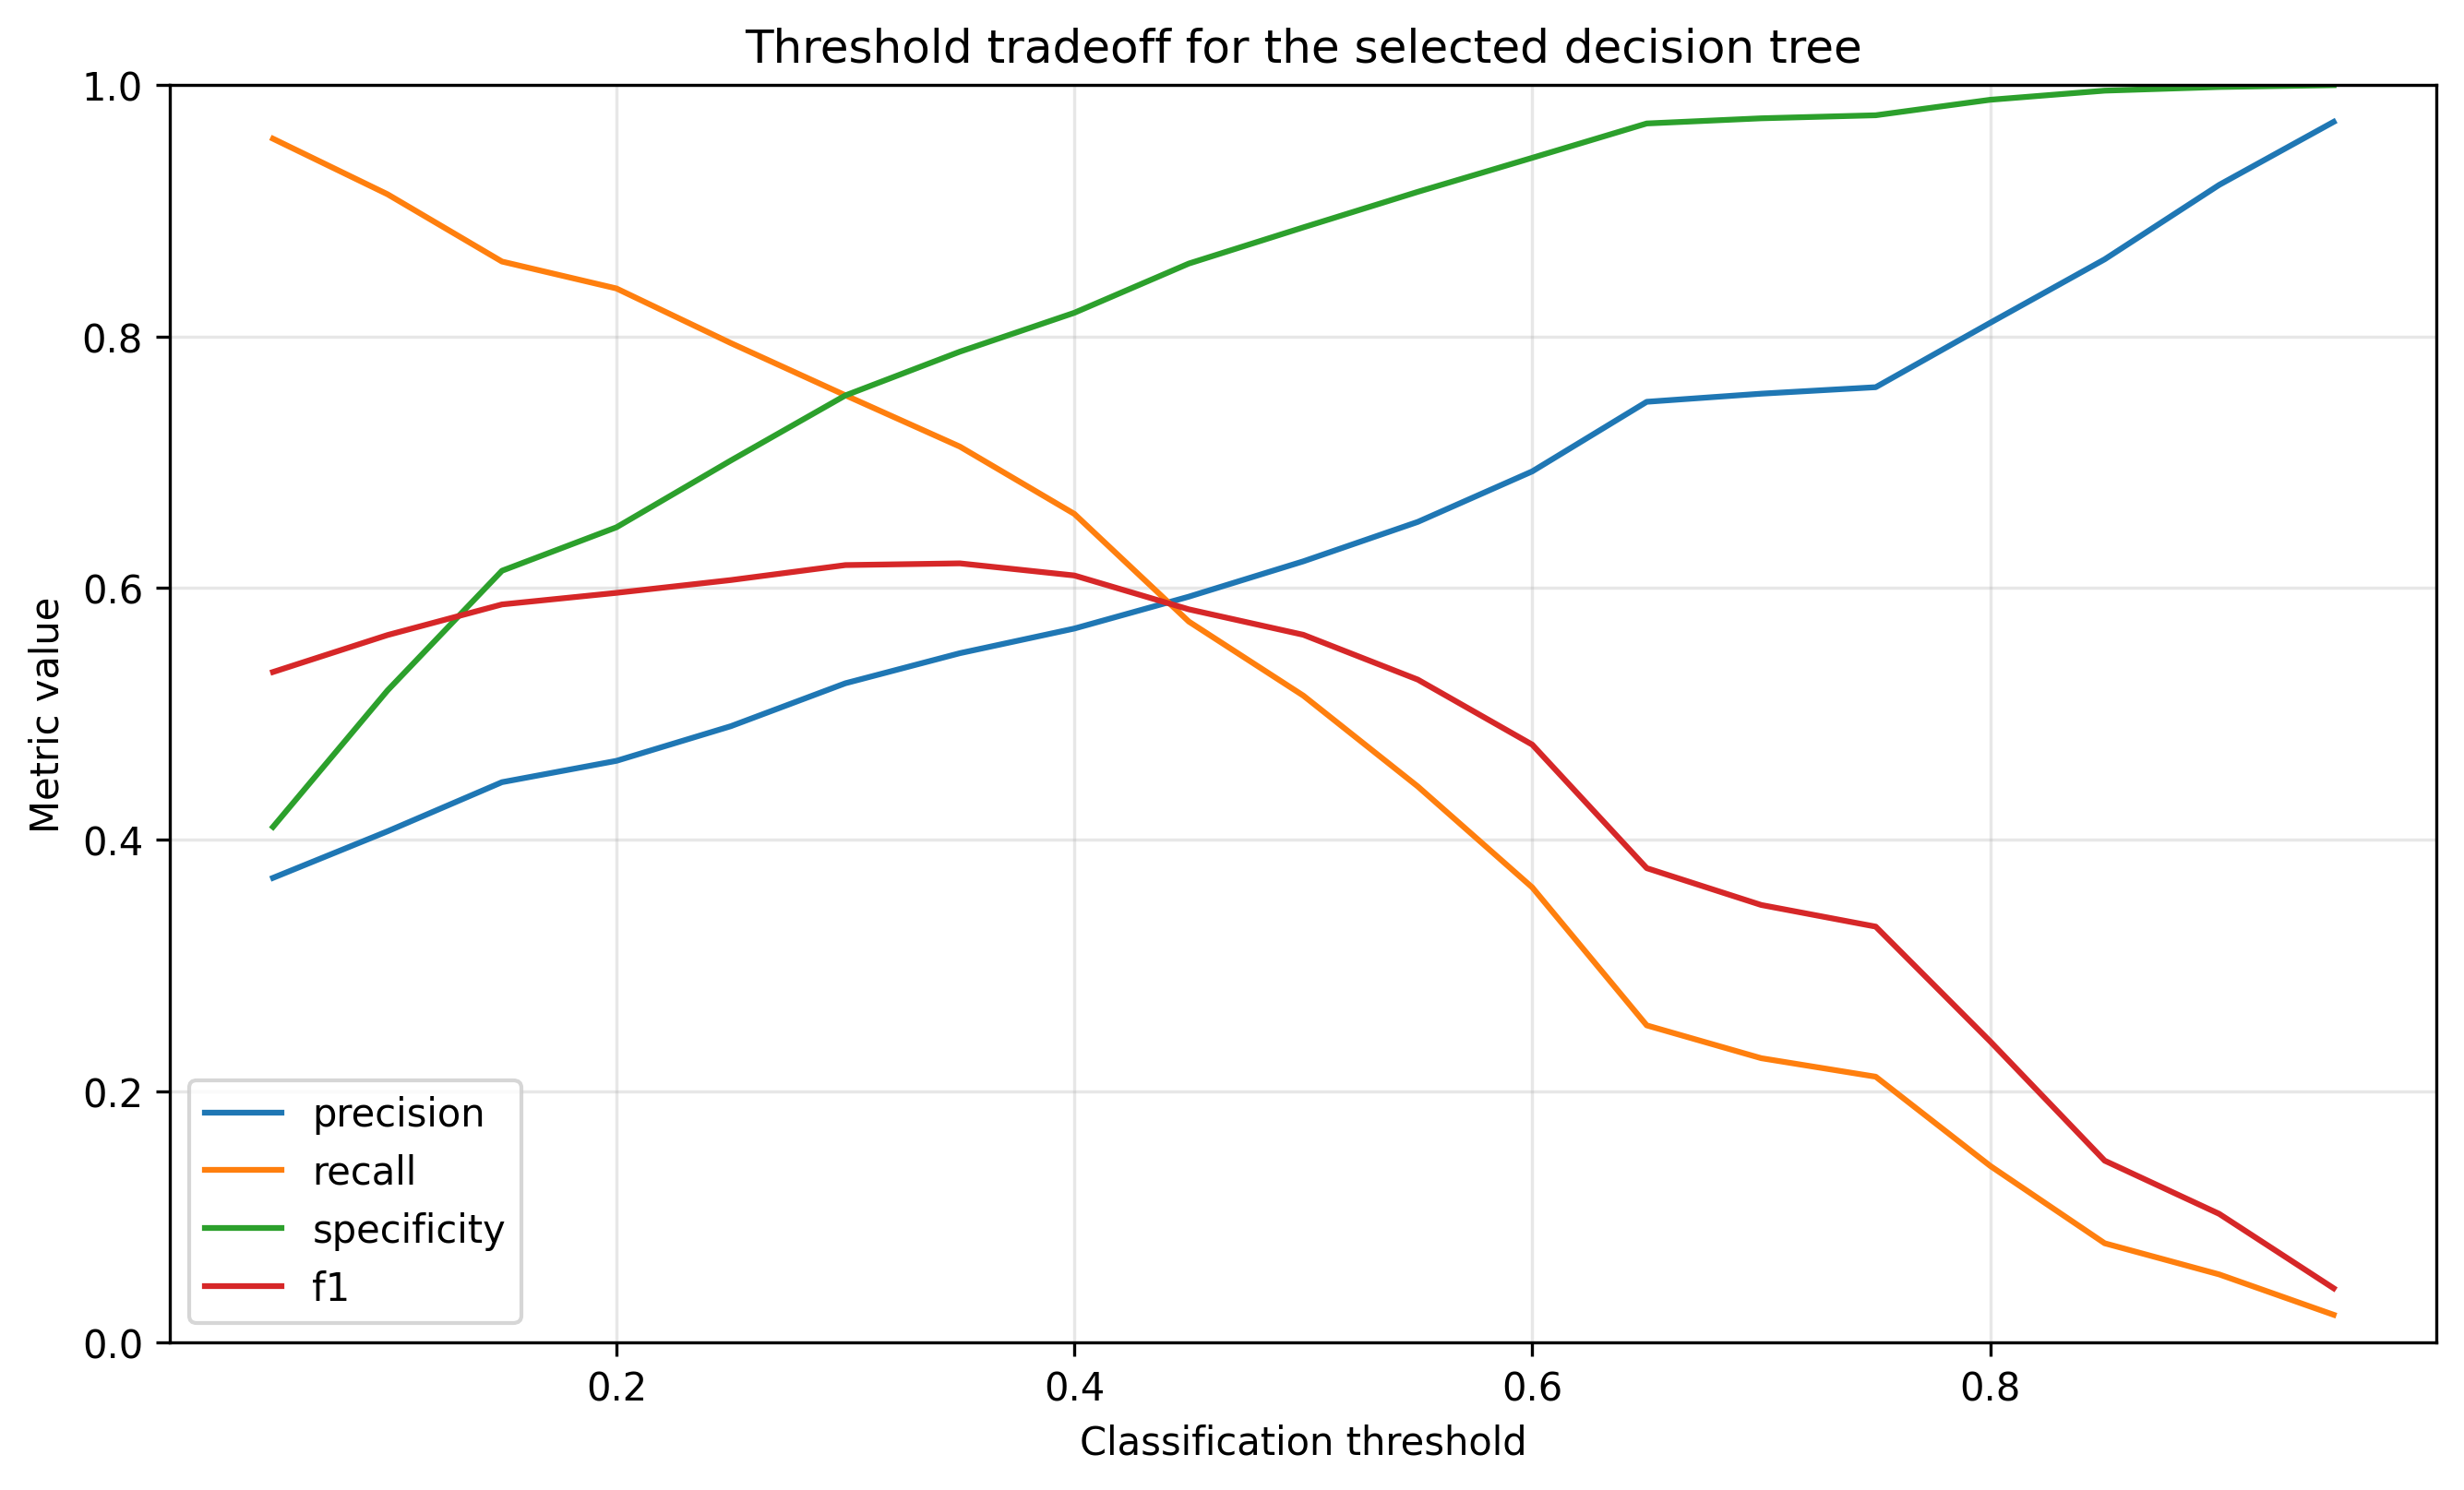
\includegraphics[width=0.88\textwidth]{../figures/decision_tree_threshold_tradeoff.png}
\caption{Threshold tradeoff for the selected decision tree}
\label{fig:decision-tree-threshold-tradeoff}
\end{figure}

At threshold \(0.30\), the selected tree has precision approximately \(0.524\), recall approximately \(0.753\), specificity approximately \(0.753\), and \(F_1\) approximately \(0.618\). At threshold \(0.35\), precision rises to approximately \(0.548\), recall is approximately \(0.712\), specificity is approximately \(0.788\), and \(F_1\) is approximately \(0.620\). At the default threshold \(0.50\), precision is approximately \(0.621\), recall falls to approximately \(0.514\), specificity rises to approximately \(0.887\), and \(F_1\) is approximately \(0.563\). This confirms again that the default threshold is not necessarily the best operating point for churn intervention.

\subsection{ROC and precision-recall curves}

Figure~\ref{fig:decision-tree-roc-curve} shows the ROC curve for the selected tree. The ROC-AUC is approximately \(0.824\), indicating useful ranking ability.

\begin{figure}[H]
\centering
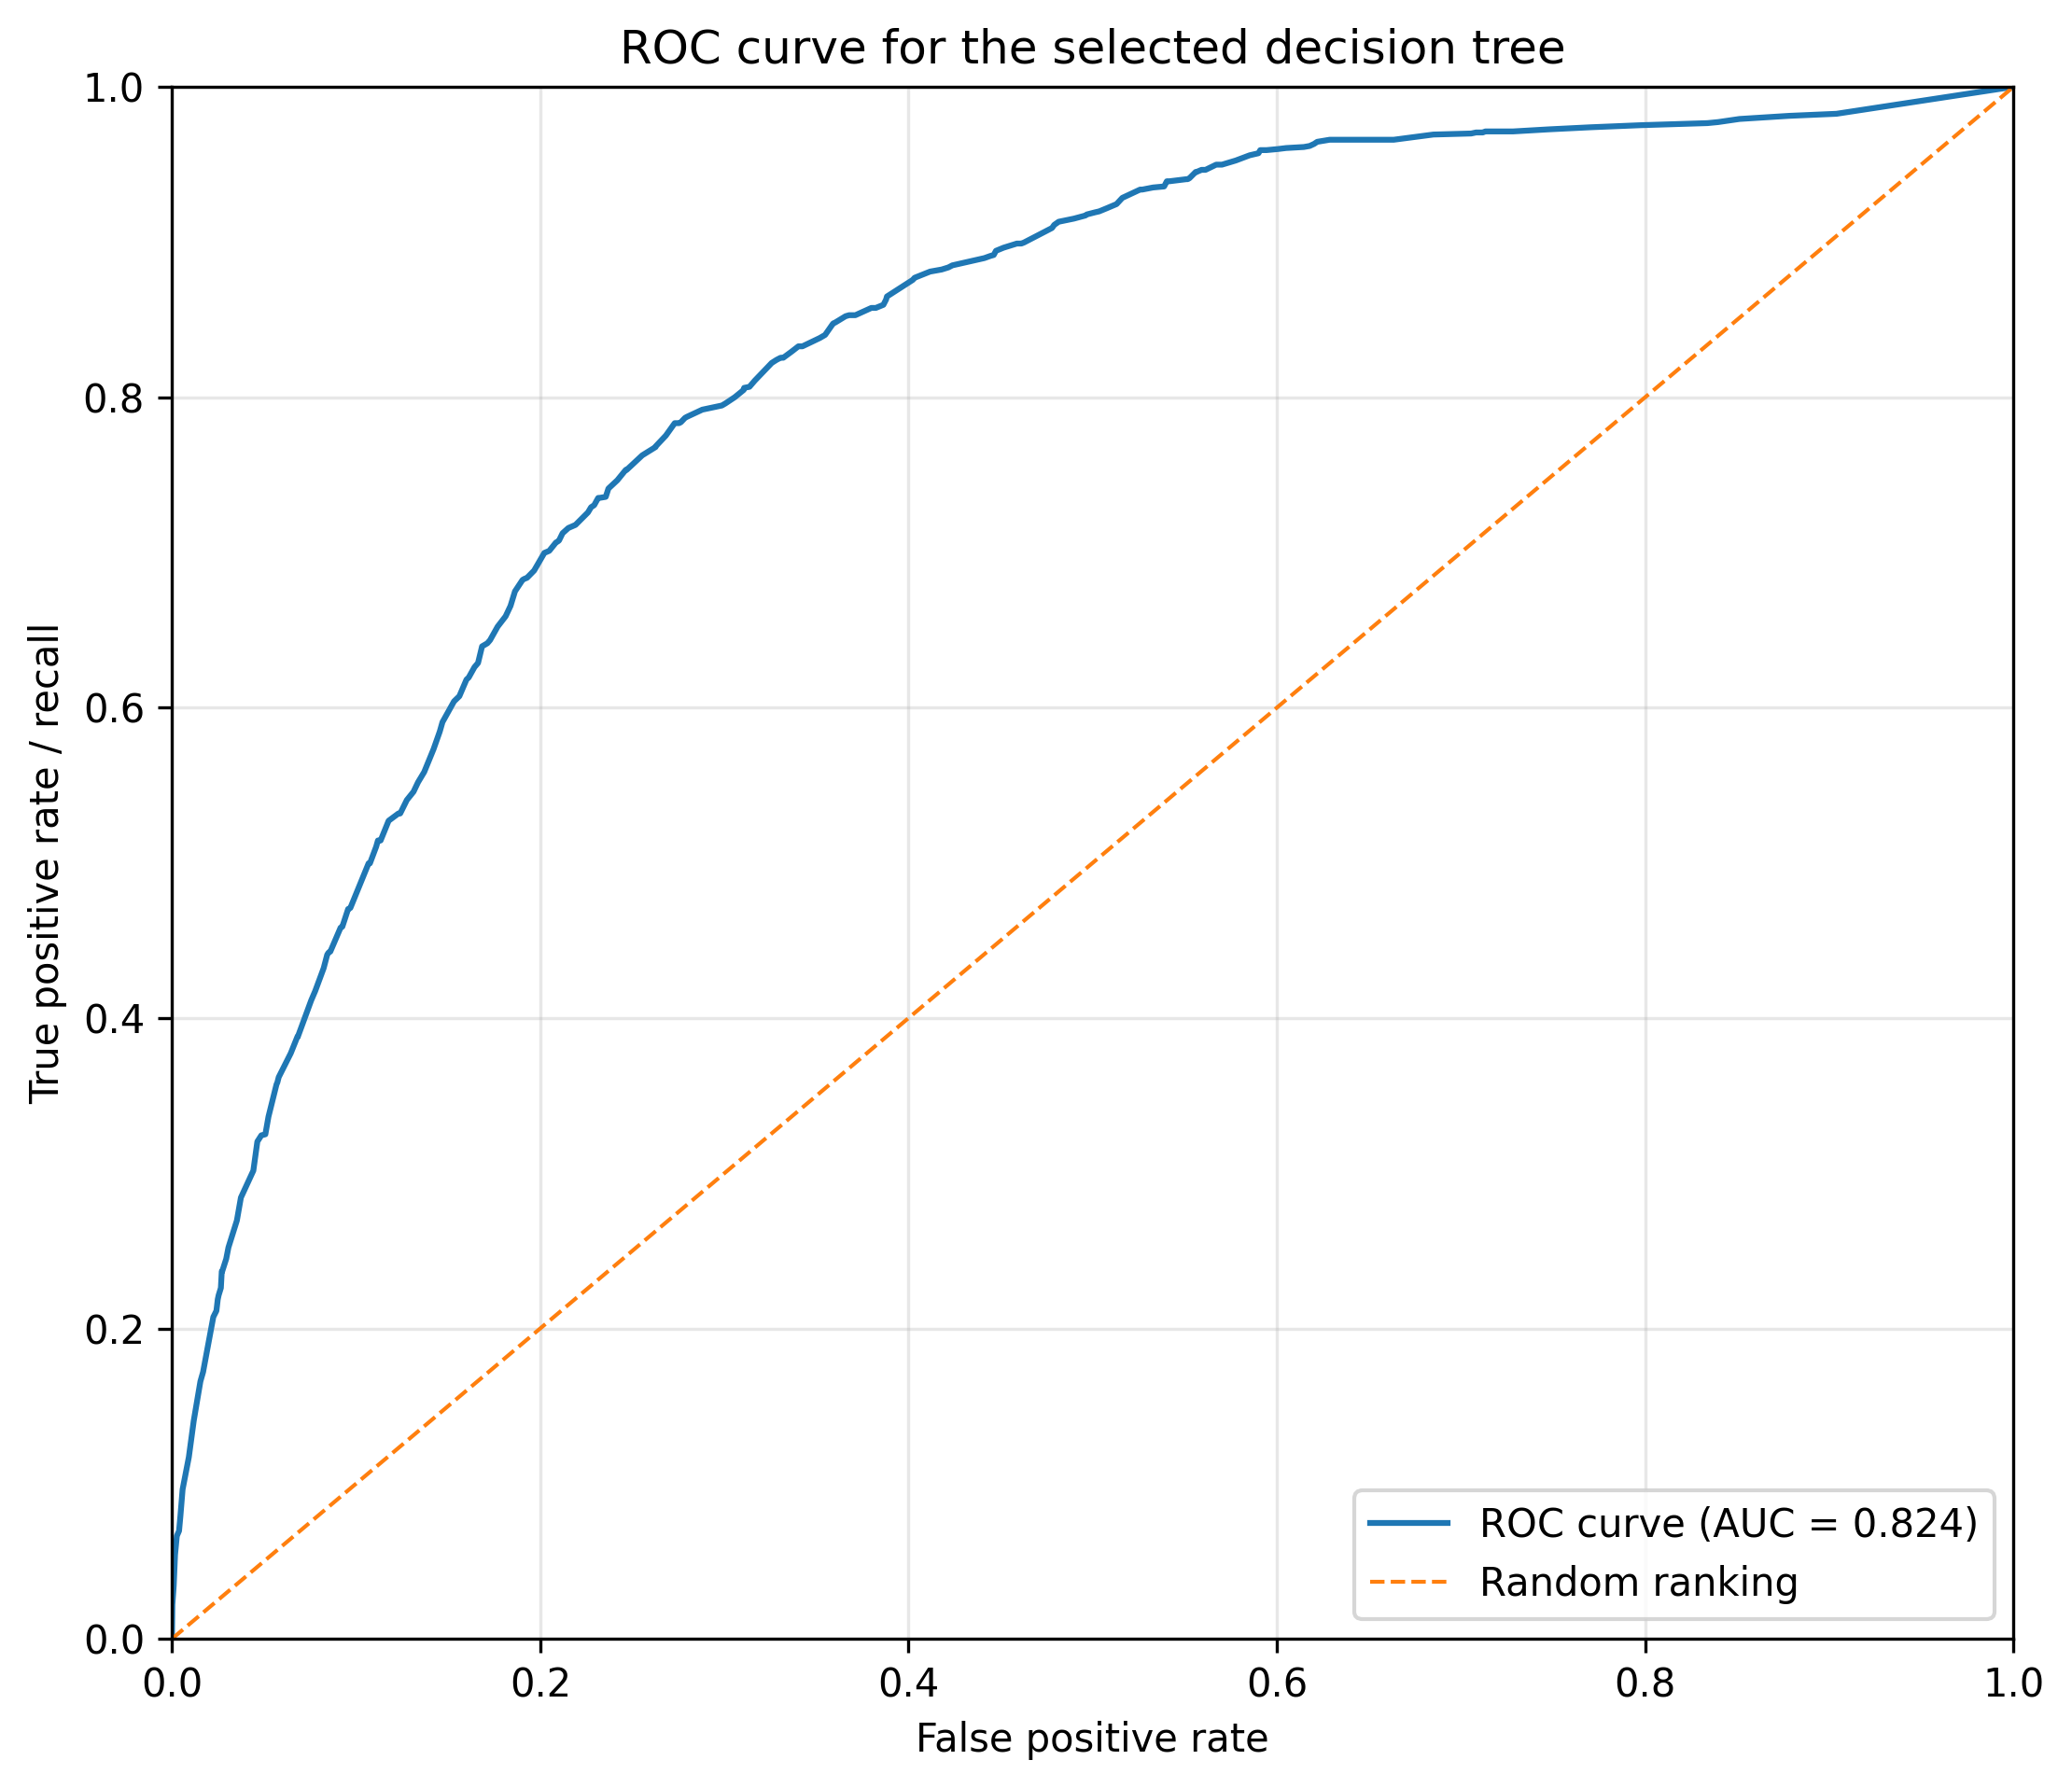
\includegraphics[width=0.72\textwidth]{../figures/decision_tree_roc_curve.png}
\caption{ROC curve for the selected decision tree}
\label{fig:decision-tree-roc-curve}
\end{figure}

Figure~\ref{fig:decision-tree-pr-curve} shows the precision-recall curve. The selected tree has PR-AUC around \(0.63\), well above the positive-rate baseline of approximately \(0.265\). This means that the tree ranks churners above non-churners much better than random ordering, even though its leaf-based probabilities produce a more stepwise ranking than smoother probabilistic models.

\begin{figure}[H]
\centering
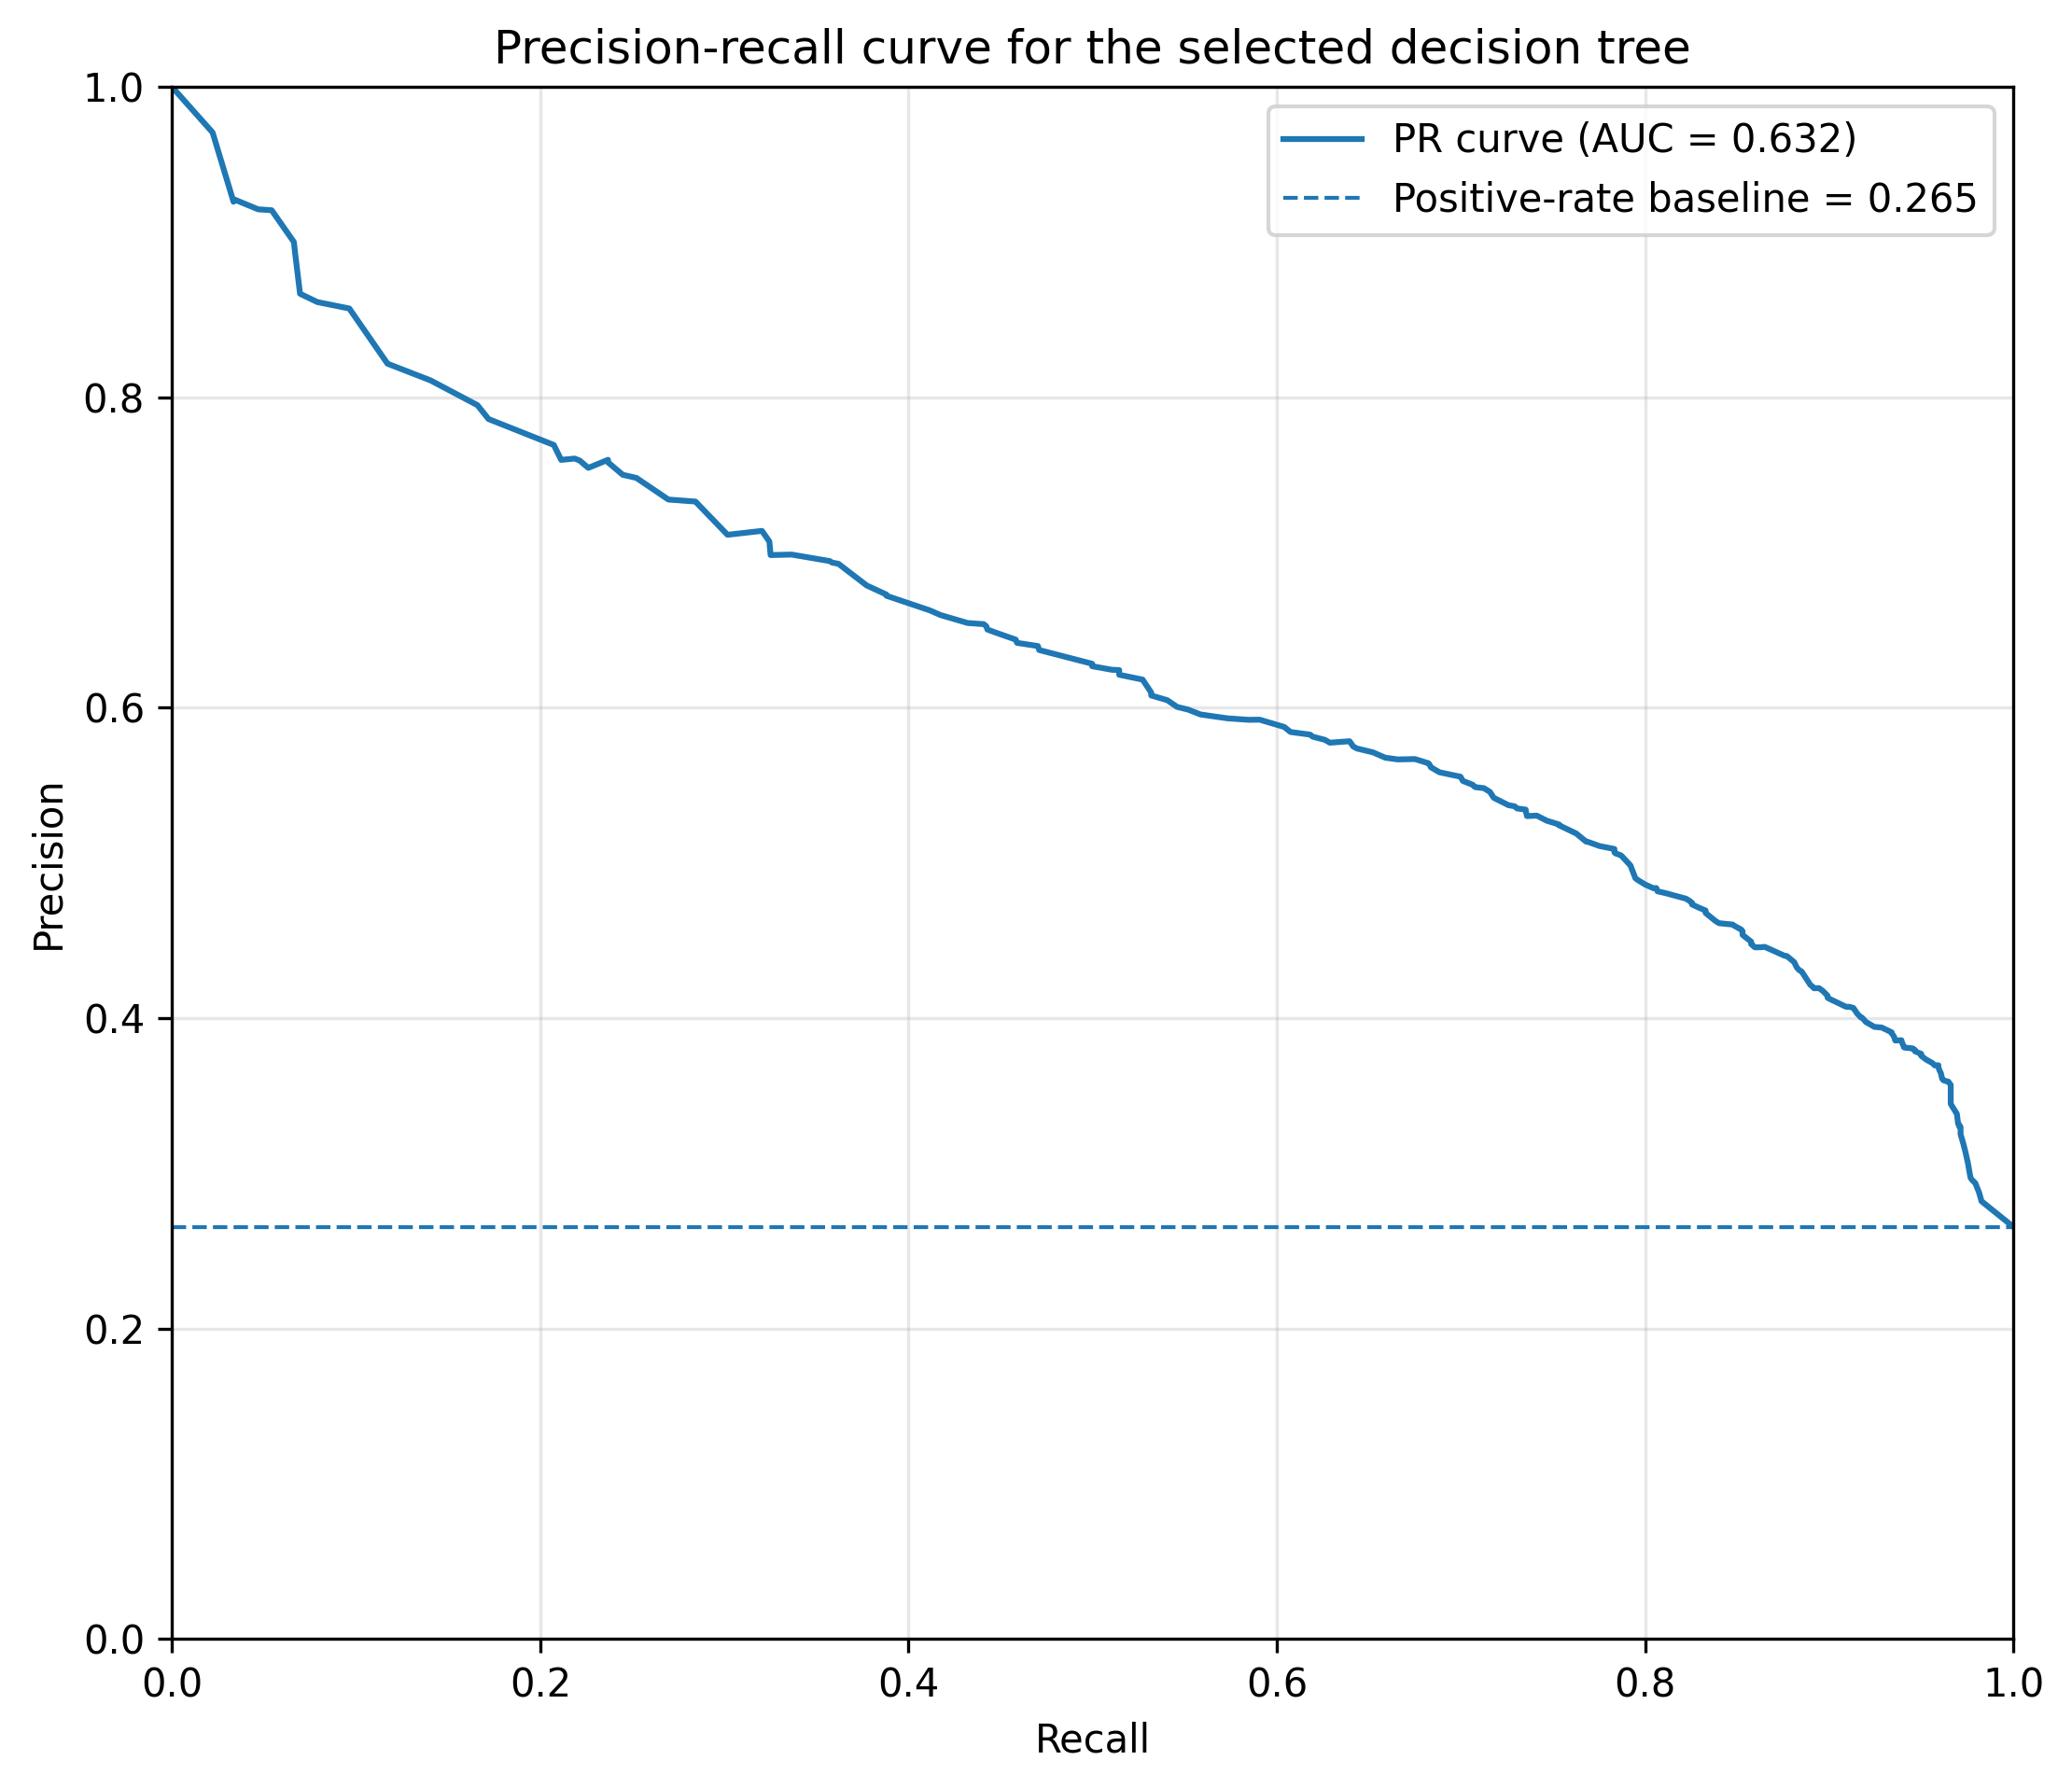
\includegraphics[width=0.72\textwidth]{../figures/decision_tree_precision_recall_curve.png}
\caption{Precision-recall curve for the selected decision tree}
\label{fig:decision-tree-pr-curve}
\end{figure}

\subsection{Interpretation of the selected tree}

The selected tree was refitted on the full training set only for interpretation. This refit is not used to estimate performance. Figure~\ref{fig:decision-tree-structure} shows the top levels of the fitted tree. The first split is on \texttt{Contract\_Month-to-month}, which is consistent with earlier EDA and logistic-regression results. Month-to-month contracts are a central churn-risk indicator.

\begin{figure}[H]
\centering
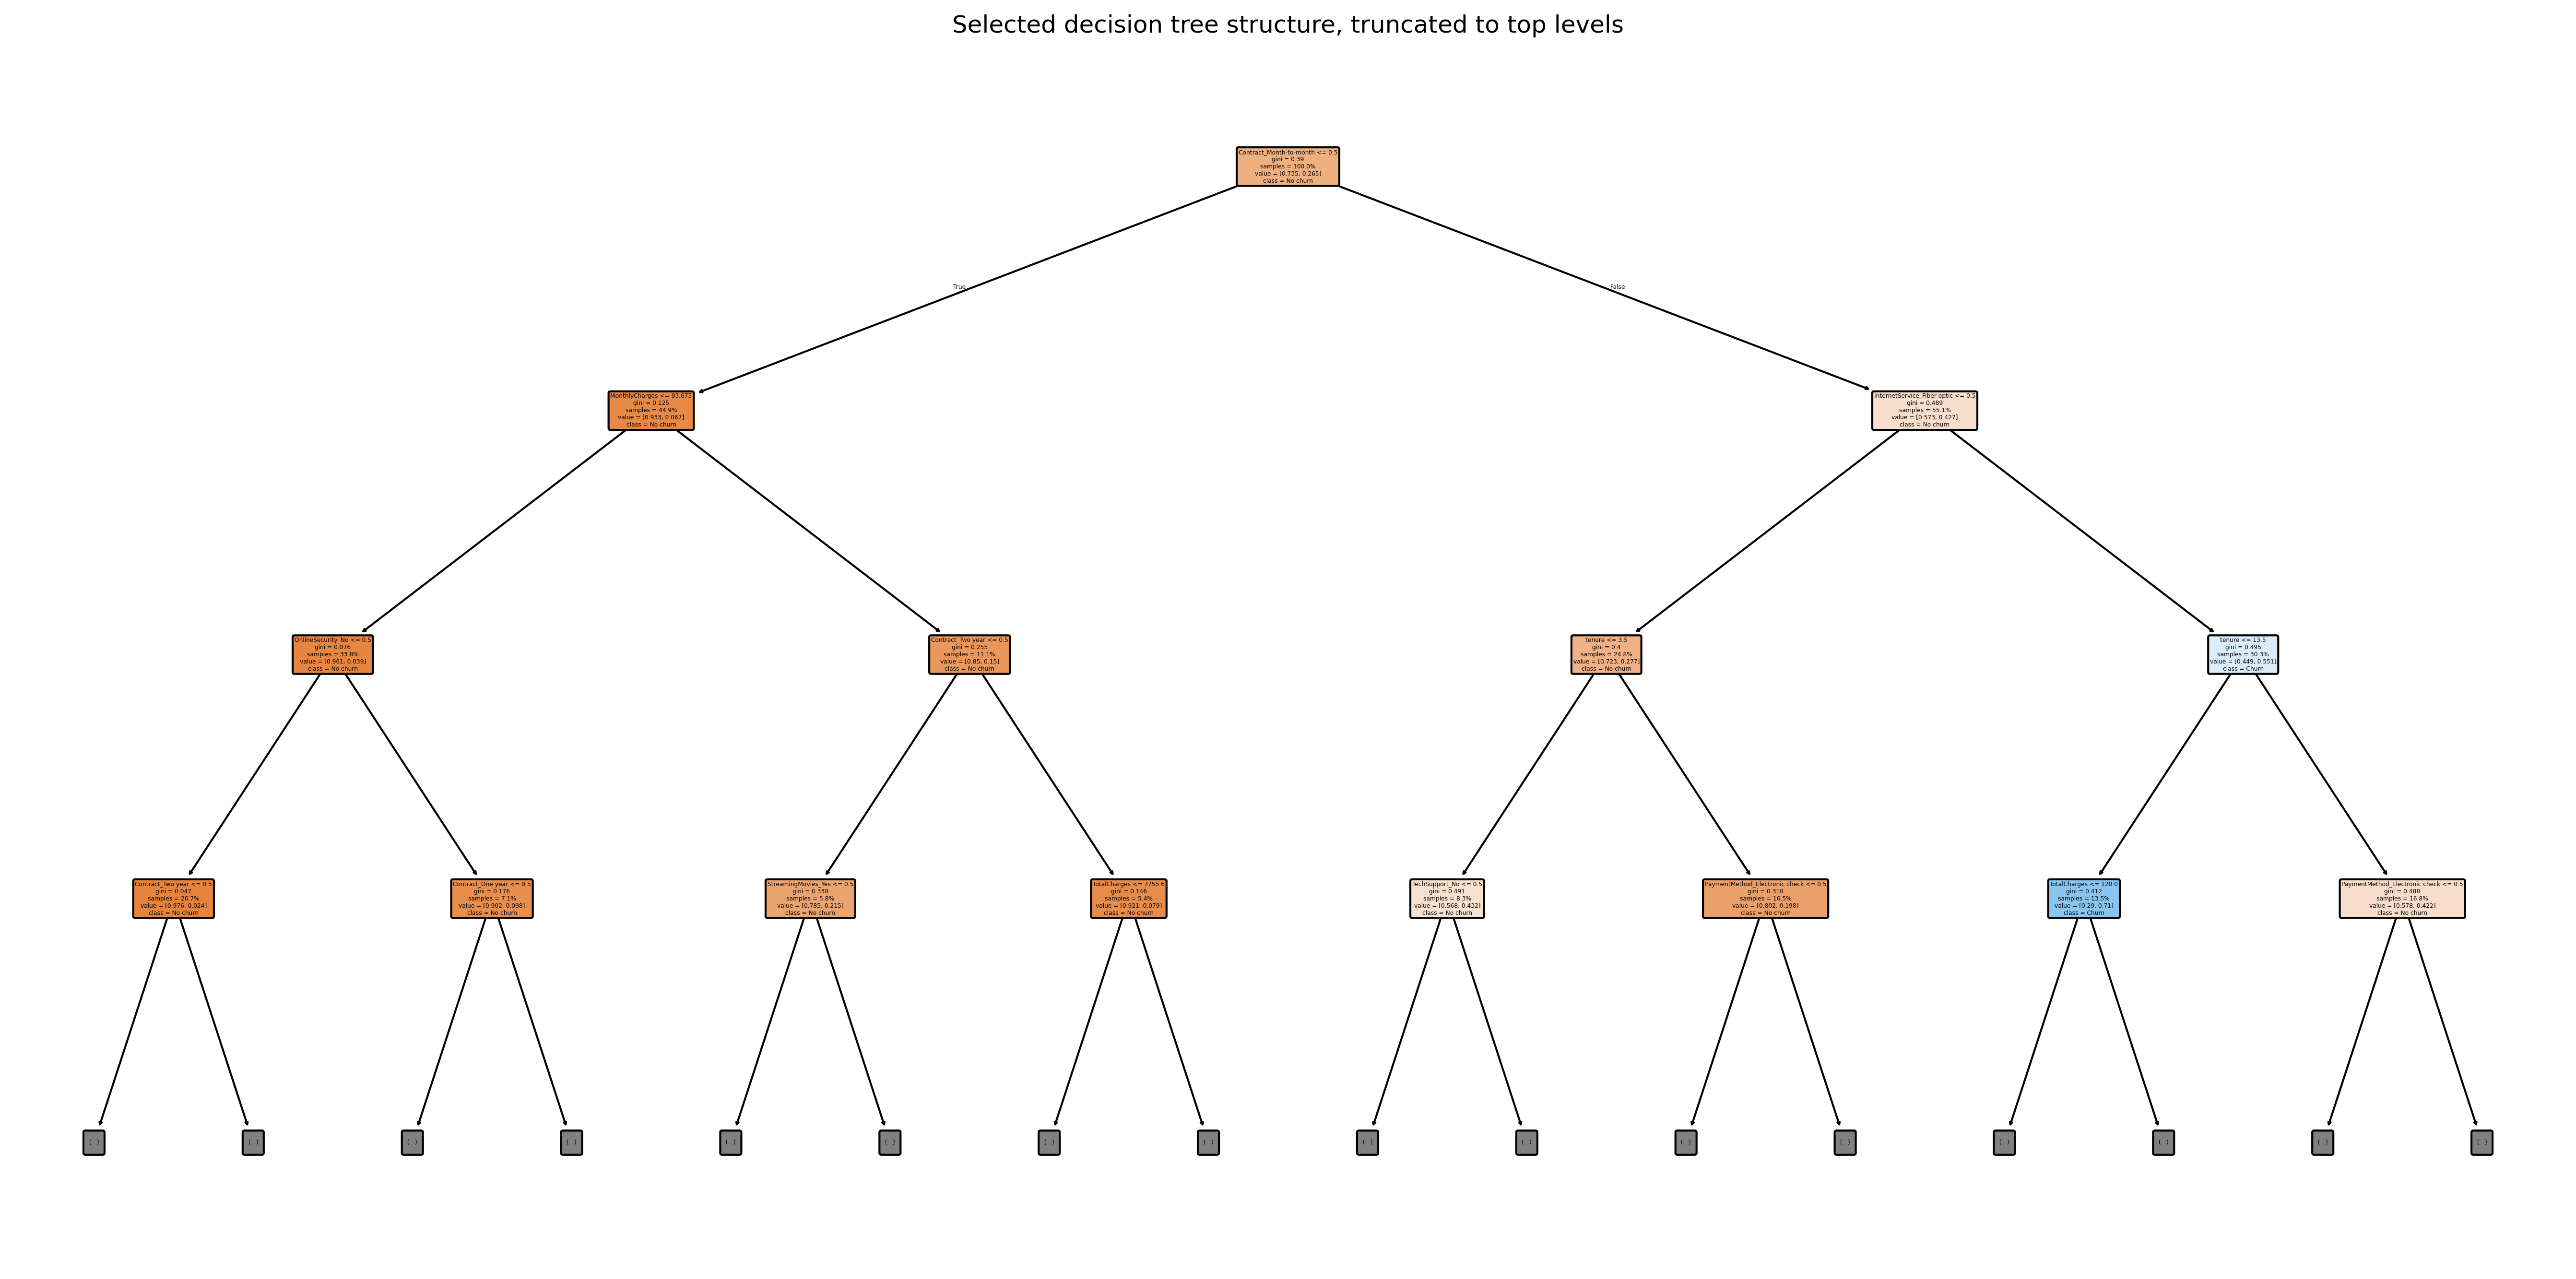
\includegraphics[width=\textwidth]{../figures/decision_tree_selected_structure.png}
\caption{Selected decision-tree structure, truncated to the top levels}
\label{fig:decision-tree-structure}
\end{figure}

Figure~\ref{fig:decision-tree-feature-importance} shows impurity-based feature importances. The dominant feature is \texttt{Contract\_Month-to-month}, followed by \texttt{InternetService\_Fiber optic}, \texttt{tenure}, \texttt{TotalCharges}, and \texttt{MonthlyCharges}. These variables are plausible churn drivers and align with previous sections.

\begin{figure}[H]
\centering
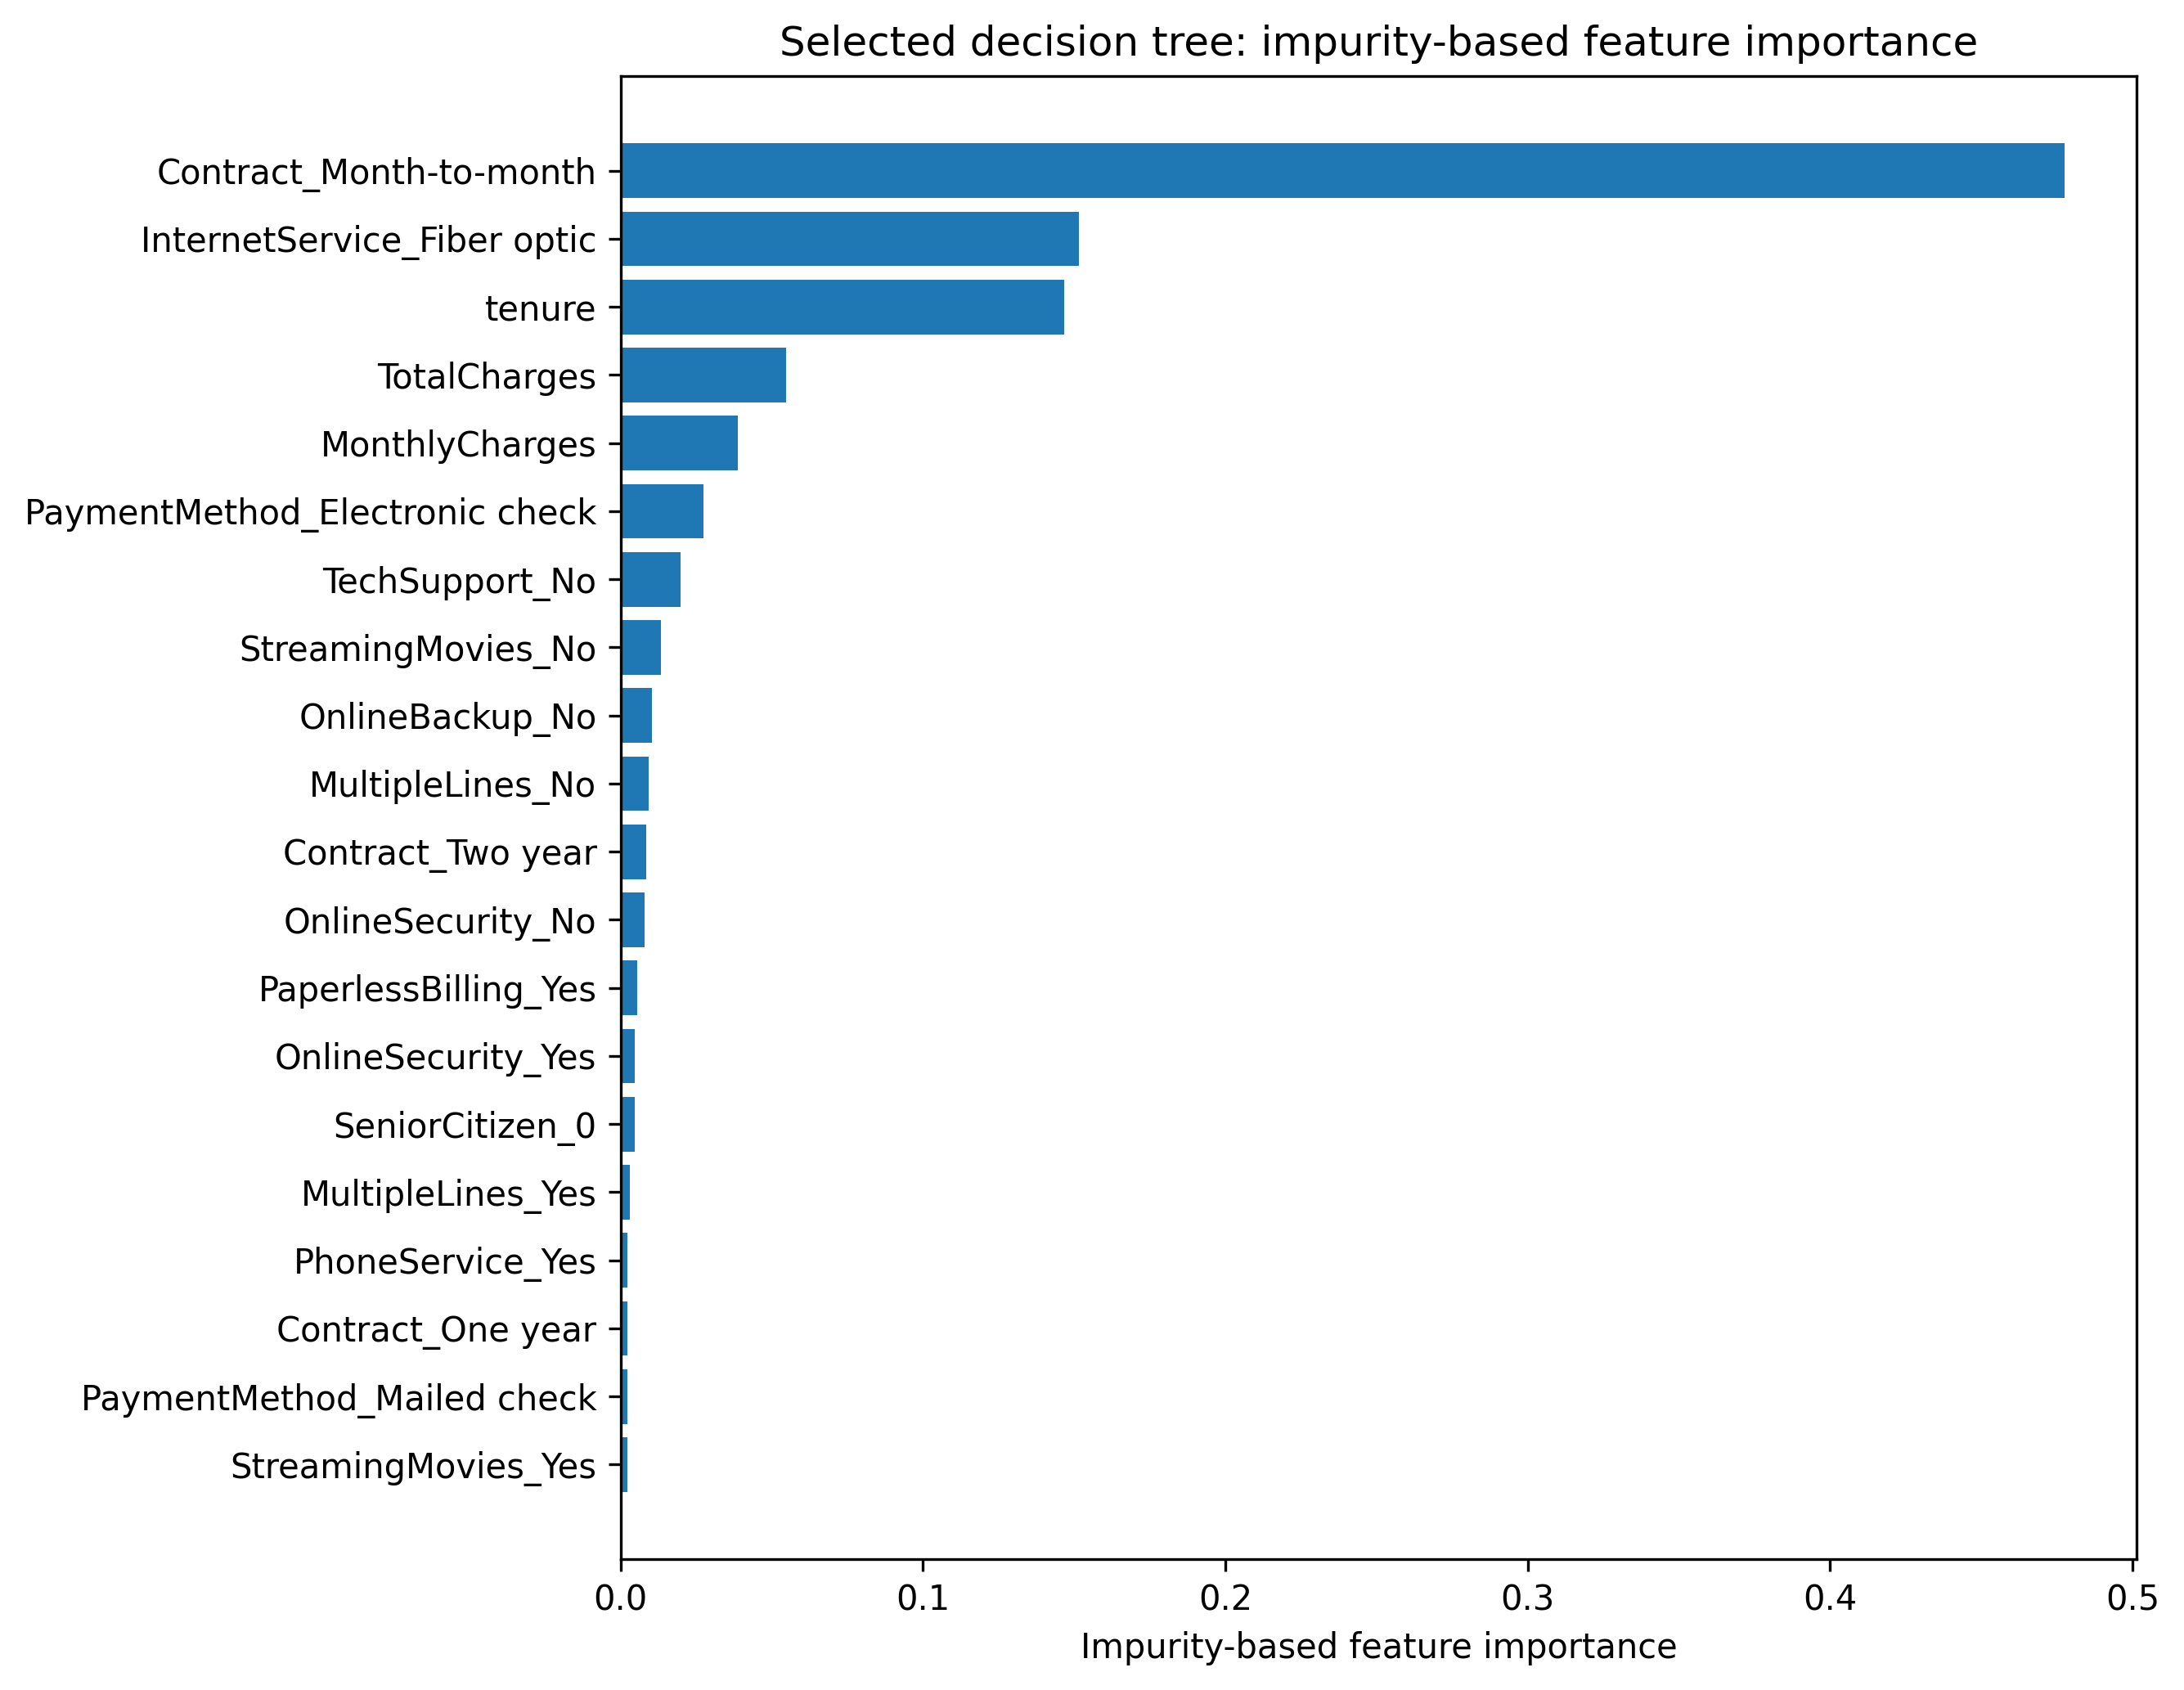
\includegraphics[width=0.82\textwidth]{../figures/decision_tree_feature_importance.png}
\caption{Impurity-based feature importance for the selected decision tree}
\label{fig:decision-tree-feature-importance}
\end{figure}

The feature-importance plot should be interpreted cautiously. Impurity-based importances reflect how much splits reduce impurity inside the fitted tree. They are not causal effects, and they can be influenced by feature cardinality, correlated predictors, and the particular tree structure. Still, they are useful for understanding which variables the selected tree uses most heavily.

\subsection{Summary}

The decision-tree section demonstrates the strengths and weaknesses of single-tree classification. A decision tree provides interpretable rule-based nonlinear classification and naturally captures interactions between features. However, the default unrestricted tree overfits and performs poorly in ranking metrics. Regularization is therefore essential.

The selected single tree is a pre-pruned Gini tree with depth 6, minimum split size 25, and minimum leaf size 10. It reaches development-stage PR-AUC around \(0.628\) and ROC-AUC around \(0.824\). This is a substantial improvement over the default unrestricted tree and a meaningful result for a transparent nonlinear model, but it does not overtake logistic regression in the current development-stage comparison.

This outcome prepares the next modelling stages. Single trees are unstable, but they are the building blocks for bagging, random forests, and boosting. The next tree-based sections can therefore ask whether aggregating many trees improves the variance, ranking quality, and robustness limitations observed here.


\newpage
\newpage
\section{Bagging and Random Forests}
\label{sec:bagging-and-random-forests}

This section evaluates bagging-based tree ensembles for churn prediction. The previous section showed that a single regularized decision tree can capture useful nonlinear structure, but a single tree remains unstable because small data changes can alter the selected splits. Bagging and random forests address this weakness by fitting many trees and averaging their predictions.

The same development discipline is used as in the previous modelling sections. The held-out test set is not used. All reported results are based on stratified cross-validation inside the training set, using out-of-fold predictions where possible. The comparisons in this section are therefore development-stage comparisons of tree-ensemble variants. They identify representative ensemble candidates within the tried configurations, but they are not final test-set performance claims.

\subsection{From one tree to an ensemble}

Let a fitted decision tree produce a churn-risk score
\[
\widehat{p}(x)
=
\widehat{P}(Y=1\mid X=x).
\]
A single tree estimates this probability from the empirical churn rate in the terminal leaf reached by customer \(x\). Because each split is chosen greedily and because terminal leaf proportions can be sensitive to the training sample, single trees often have high variance.

An ensemble reduces this instability by fitting many trees and averaging their predictions. If \(B\) trees are fitted and tree \(b\) produces score \(\widehat{p}_b(x)\), the ensemble score is
\[
\widehat{p}_{\mathrm{ens}}(x)
=
\frac{1}{B}
\sum_{b=1}^{B}
\widehat{p}_b(x).
\]
The corresponding hard prediction at threshold \(t\) is
\[
\widehat{y}(x;t)
=
\mathbb{1}\{\widehat{p}_{\mathrm{ens}}(x)\geq t\}.
\]
Thus, the ensemble remains a probability-scoring classifier. Ranking metrics such as ROC-AUC and PR-AUC can be computed from \(\widehat{p}_{\mathrm{ens}}(x)\), while hard classification metrics depend on the chosen threshold.

\subsection{Bagging of decision trees}

Bagging, short for bootstrap aggregation, fits each tree on a bootstrap-resampled version of the training data. For each ensemble member \(b=1,\ldots,B\), a bootstrap sample
\[
\mathcal{D}^{*(b)}
=
\{(x_i^{*(b)},y_i^{*(b)})\}_{i=1}^{n_b}
\]
is drawn with replacement from the original training data. A decision tree \(h_b\) is fitted on this resampled dataset. Predictions are then averaged across all trees.

The main idea is variance reduction. Averaging many noisy predictors can be much more stable than using one noisy predictor. However, the reduction depends on how correlated the tree predictions are. If all trees make almost the same errors, averaging helps only a little. If the trees are diverse but still individually useful, averaging helps more.

In the bagged-tree variant used here, the base learner is a \texttt{DecisionTreeClassifier} inside scikit-learn's \texttt{BaggingClassifier}. The model uses bootstrap sampling across observations, while each tree can still consider all available features when choosing splits.

\subsection{Random forests as a bagging-based extension}

A random forest is a specialized bagging-based tree ensemble. Like plain bagging, it fits many trees on bootstrap-resampled training datasets. The additional random-forest idea is feature subsampling at each split. Instead of allowing every split to search over all \(p\) available features, each split considers only a random subset of features.

This extra randomness is designed to reduce correlation between trees. If one strong predictor dominates the split search, many bagged trees may look similar. Random feature subsampling forces different trees to explore different predictors and interactions. The ensemble average can then benefit more from diversification.

The distinction in this section is therefore not between unrelated model families. The comparison is between two tree-ensemble variants:

\begin{itemize}[leftmargin=*]
    \item \textbf{Plain bagged trees}: bootstrap-resampled decision trees where each split can consider all features.
    \item \textbf{Random forests}: bootstrap-resampled decision trees with additional random feature subsampling at each split.
\end{itemize}

\subsection{Out-of-bag observations}

Bootstrap sampling leaves out some observations from each tree's bootstrap sample. For a given tree \(b\), observations not included in \(\mathcal{D}^{*(b)}\) are called out-of-bag observations for that tree. These observations can be used to form out-of-bag predictions, because they were not used to train that particular tree.

Out-of-bag diagnostics are useful for tree ensembles because they provide an internal validation signal. In this project, however, out-of-bag scores are treated as supplementary diagnostics rather than as the main selection criterion. The main development comparisons still use the same stratified cross-validation framework as the earlier model sections, so that model-family results remain comparable.

\subsection{Hyperparameter tuning strategy}

Several valid strategies exist for hyperparameter tuning. Examples include fixed grid search, random search, Bayesian or Optuna-style optimization, successive halving, repeated cross-validation, and nested cross-validation. These strategies answer slightly different practical questions and have different computational costs.

This section uses transparent fixed grids. This choice is deliberate. The purpose here is model-family learning and controlled development-stage comparison, not final exhaustive optimization. A fixed grid makes it easy to see how the number of trees, bootstrap sample size, tree depth, leaf size, and feature subsampling affect performance. Later, after all model families have been studied, stronger training-only comparison procedures such as repeated cross-validation, paired comparisons, nested cross-validation, or more adaptive search can be used for serious final candidates.

The selected rows in this section should therefore be interpreted as the strongest configurations within the tried development grids, not as globally optimal hyperparameters and not as statistical proof of superiority.

\subsection{Experimental design}

The experiments compare four relevant models:

\begin{itemize}[leftmargin=*]
    \item the selected single decision tree from Section~\ref{sec:decision-trees};
    \item a plain bagged-tree ensemble selected from a fixed development grid;
    \item a default random forest with 100 trees;
    \item a random forest selected from a fixed development grid.
\end{itemize}

PR-AUC remains the primary development ranking metric because churn is the minority class and positive-class retrieval is central to the project. Balanced accuracy and \(F_1\) are retained as secondary threshold-dependent summaries. The final model selection stage will later revisit the strongest candidates across model families using a more careful training-only comparison.

\subsection{Bagging grid results}

Figure~\ref{fig:bagging-pr-auc-by-estimators} shows the bagged-tree grid from the perspective of PR-AUC. The results are stable across the evaluated ensemble sizes. Increasing the number of trees from 50 to 100 and 200 produces only small changes, which indicates that the ensemble has already largely stabilized within this range.

\begin{figure}[H]
\centering
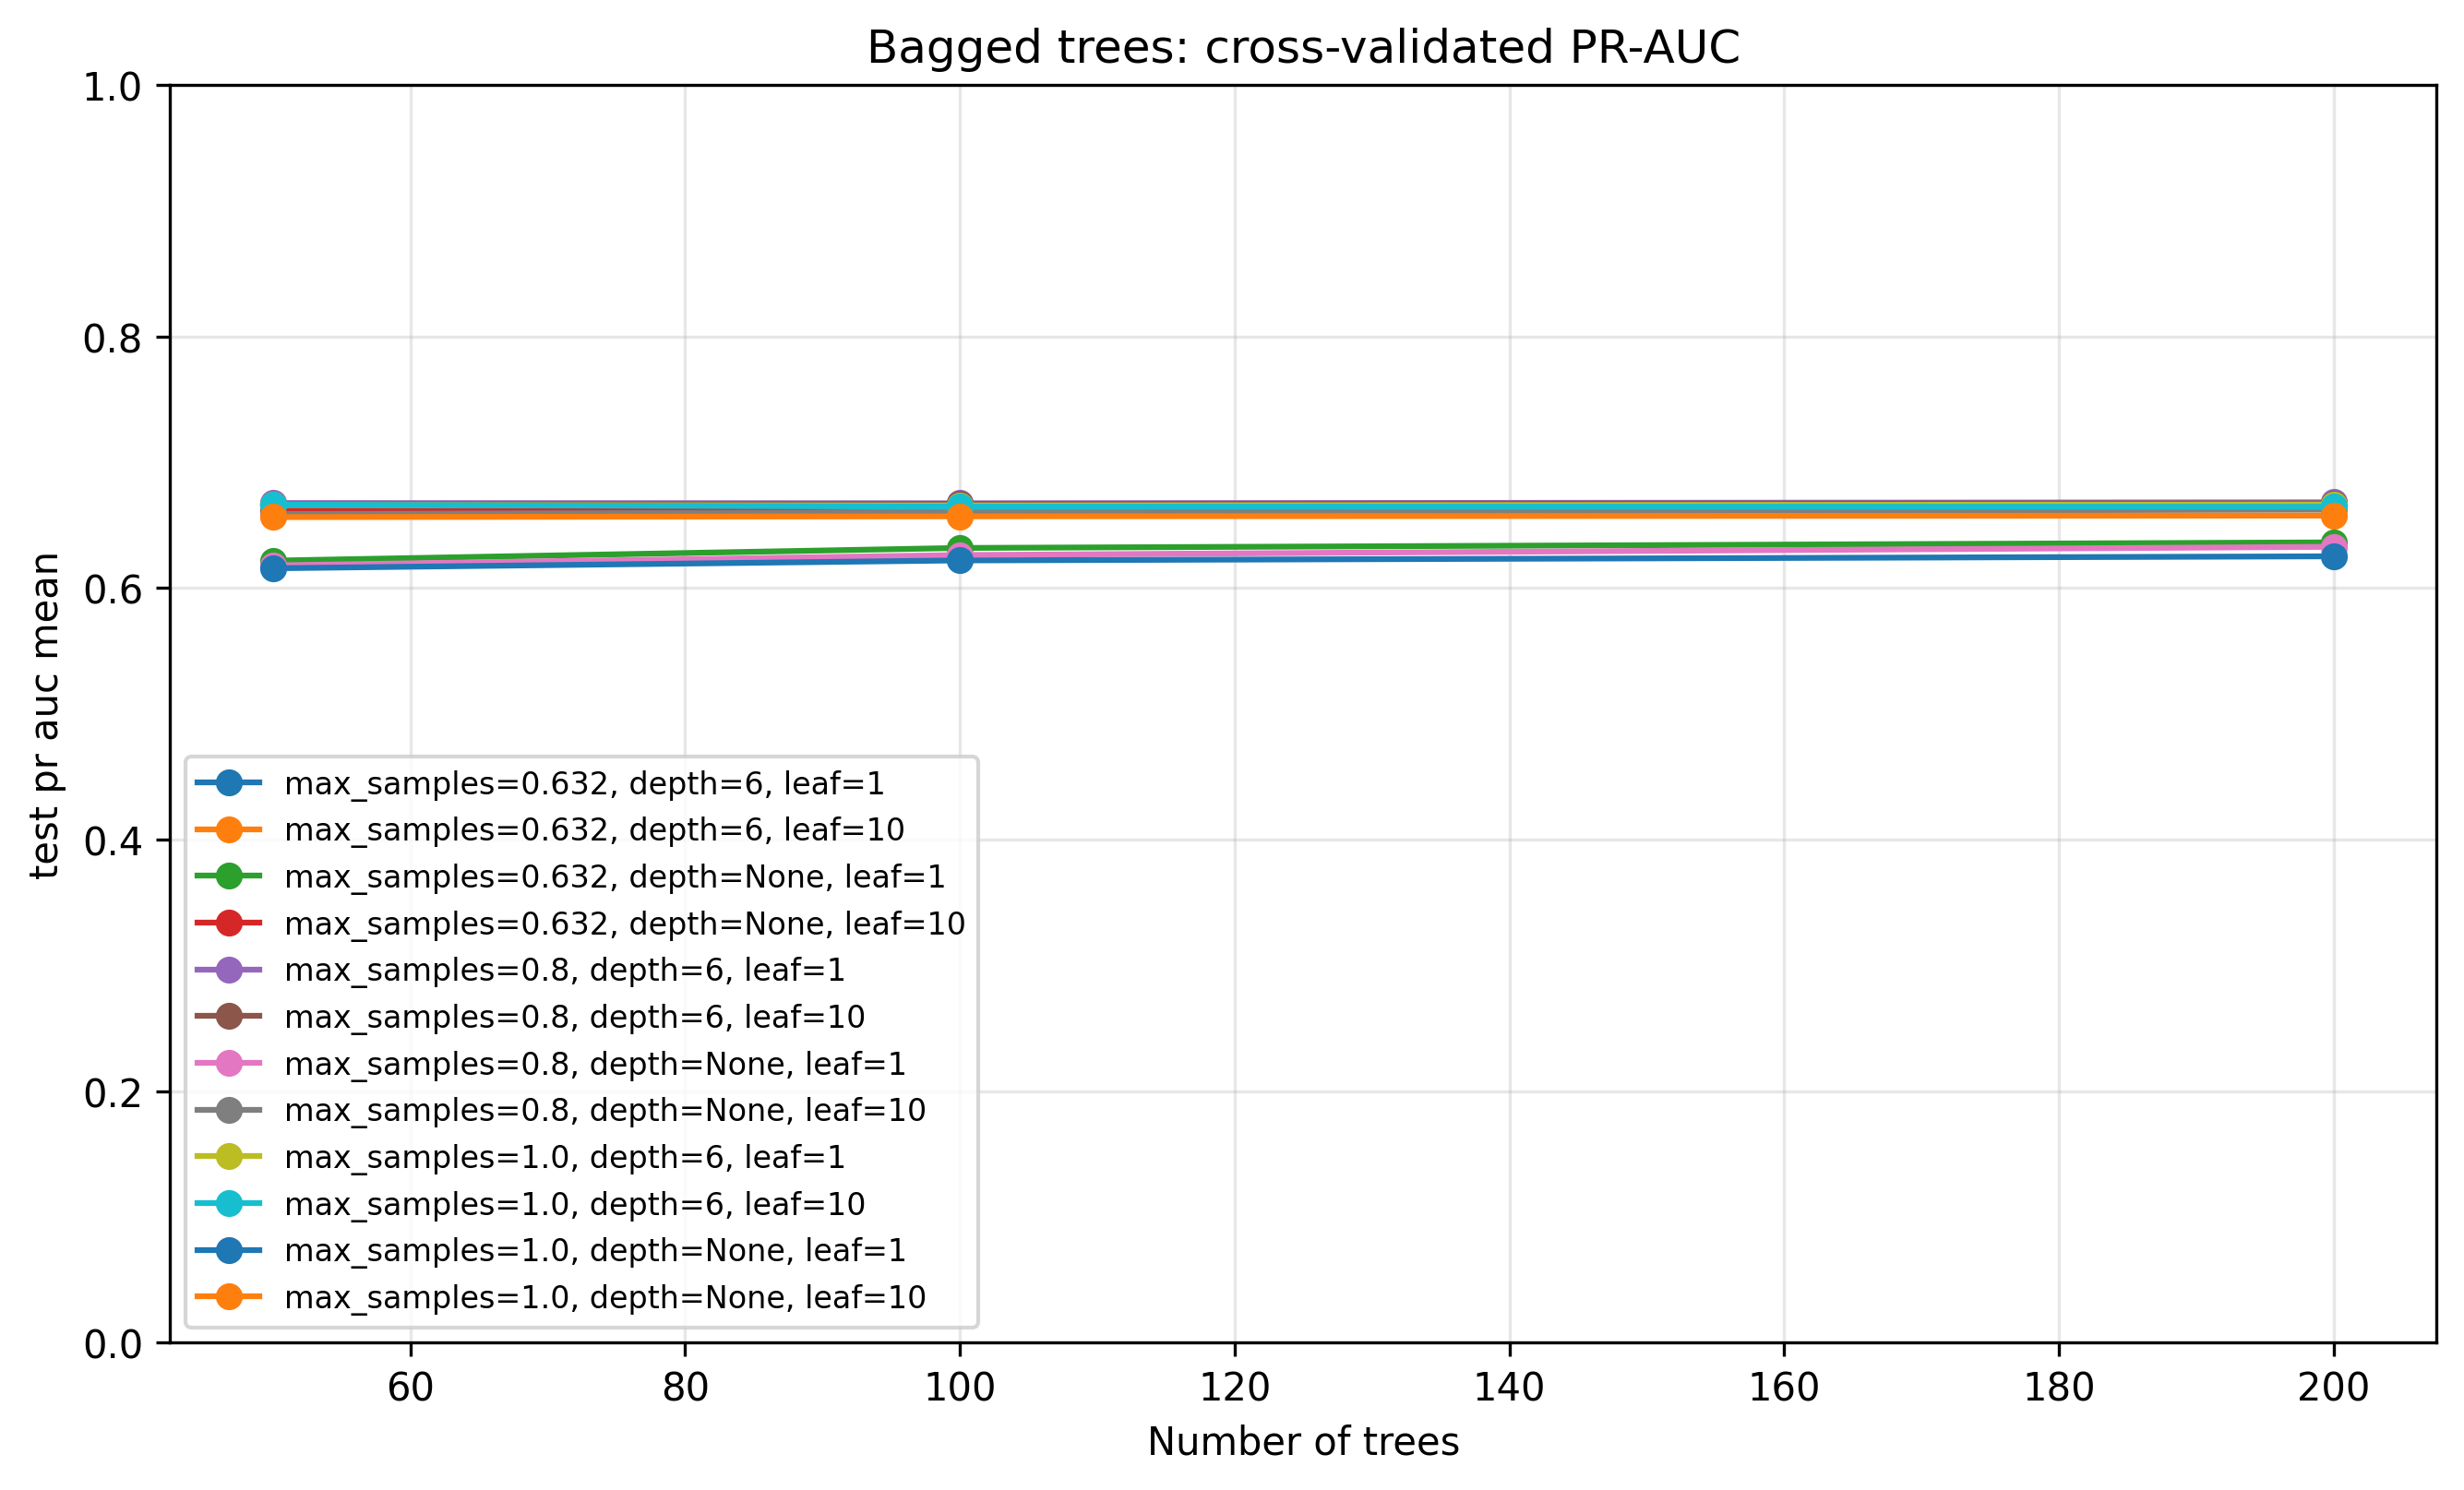
\includegraphics[width=0.88\textwidth]{../figures/bagging_pr_auc_by_estimators.png}
\caption{Bagged trees: cross-validated PR-AUC by number of trees}
\label{fig:bagging-pr-auc-by-estimators}
\end{figure}

The best bagged-tree candidate in the fixed grid uses 200 trees, \(\texttt{max\_samples}=0.8\), base-tree maximum depth 6, and base-tree \(\texttt{min\_samples\_leaf}=1\). Its grid-level mean PR-AUC is approximately \(0.668\). The small differences across neighbouring configurations should not be overinterpreted. The more important result is that bagging improves the single-tree ranking performance by averaging many bootstrapped trees.

Figure~\ref{fig:bagging-balanced-accuracy-by-estimators} shows the same bagging grid using balanced accuracy. The pattern is also flat across ensemble sizes, with values around \(0.70\). This supports the same interpretation: within the tried range, the exact number of trees matters less than the move from one tree to an averaged ensemble.

\begin{figure}[H]
\centering
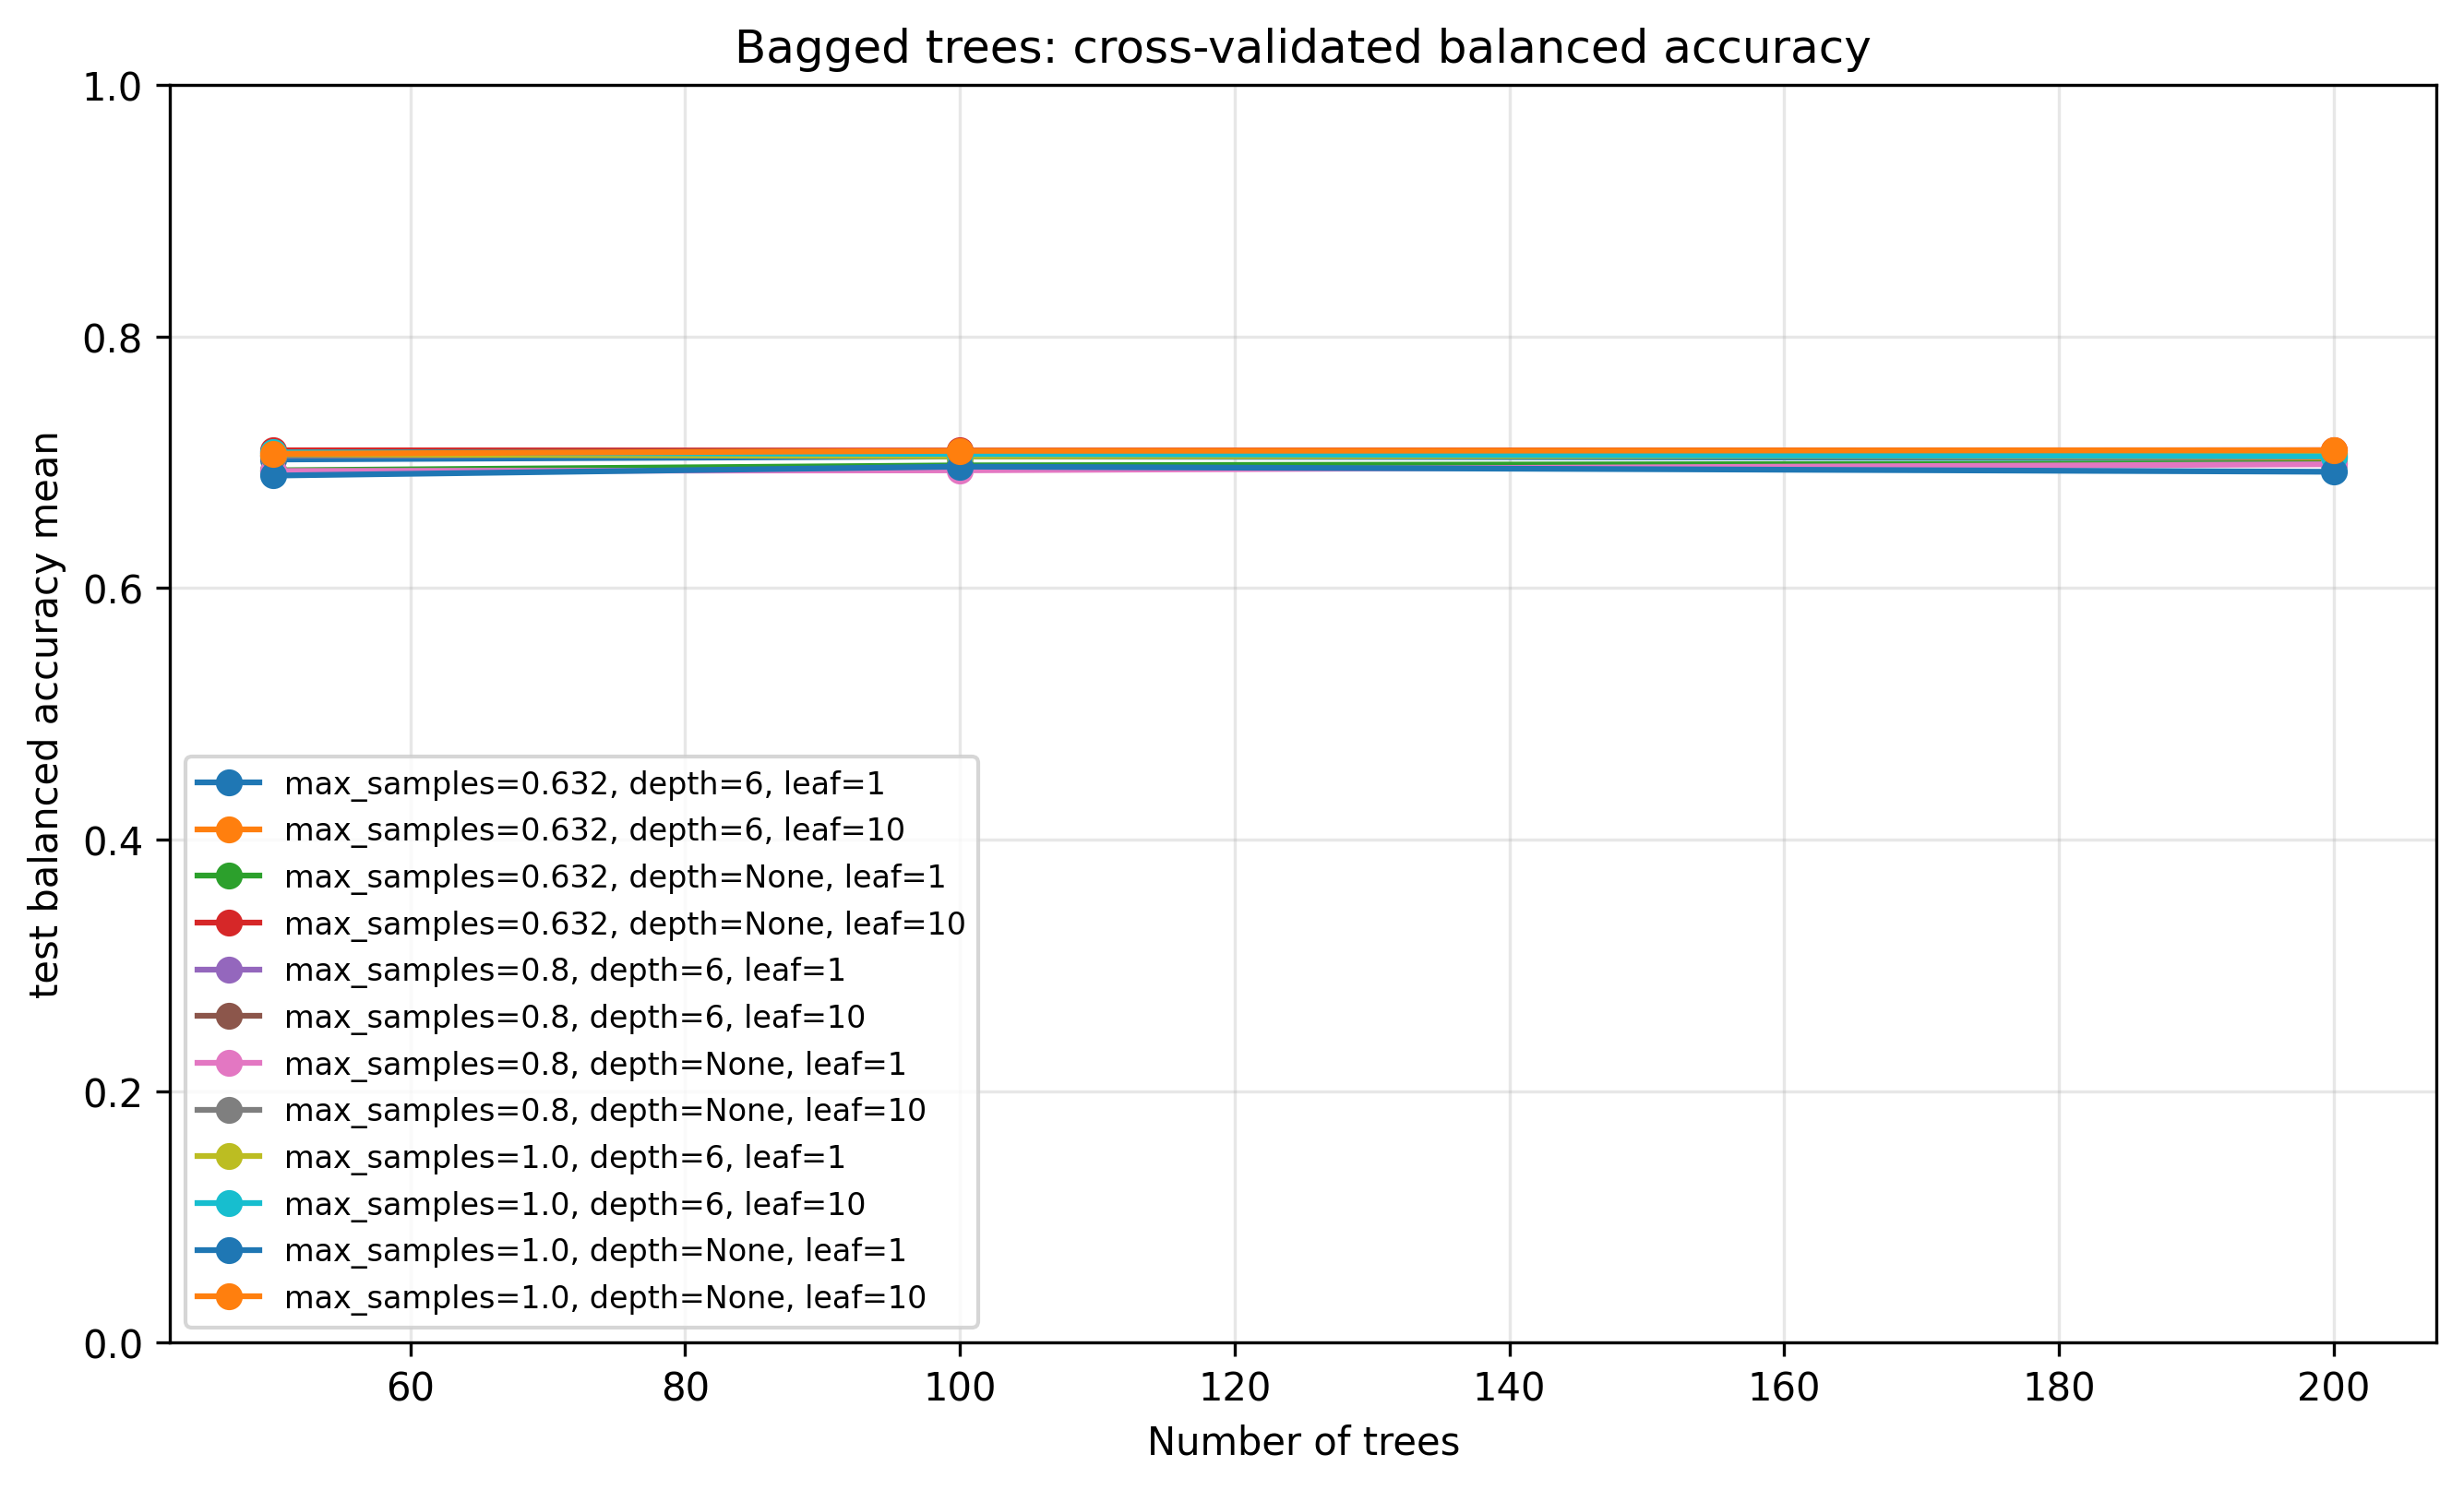
\includegraphics[width=0.88\textwidth]{../figures/bagging_balanced_accuracy_by_estimators.png}
\caption{Bagged trees: cross-validated balanced accuracy by number of trees}
\label{fig:bagging-balanced-accuracy-by-estimators}
\end{figure}

\subsection{Random-forest grid results}

Figure~\ref{fig:random-forest-pr-auc-by-depth} shows the random-forest grid from the perspective of PR-AUC. The strongest random-forest candidate uses 200 trees, maximum depth 10, \(\texttt{min\_samples\_leaf}=10\), and \(\texttt{max\_features}=\texttt{sqrt}\). Its grid-level mean PR-AUC is approximately \(0.664\).

\begin{figure}[H]
\centering
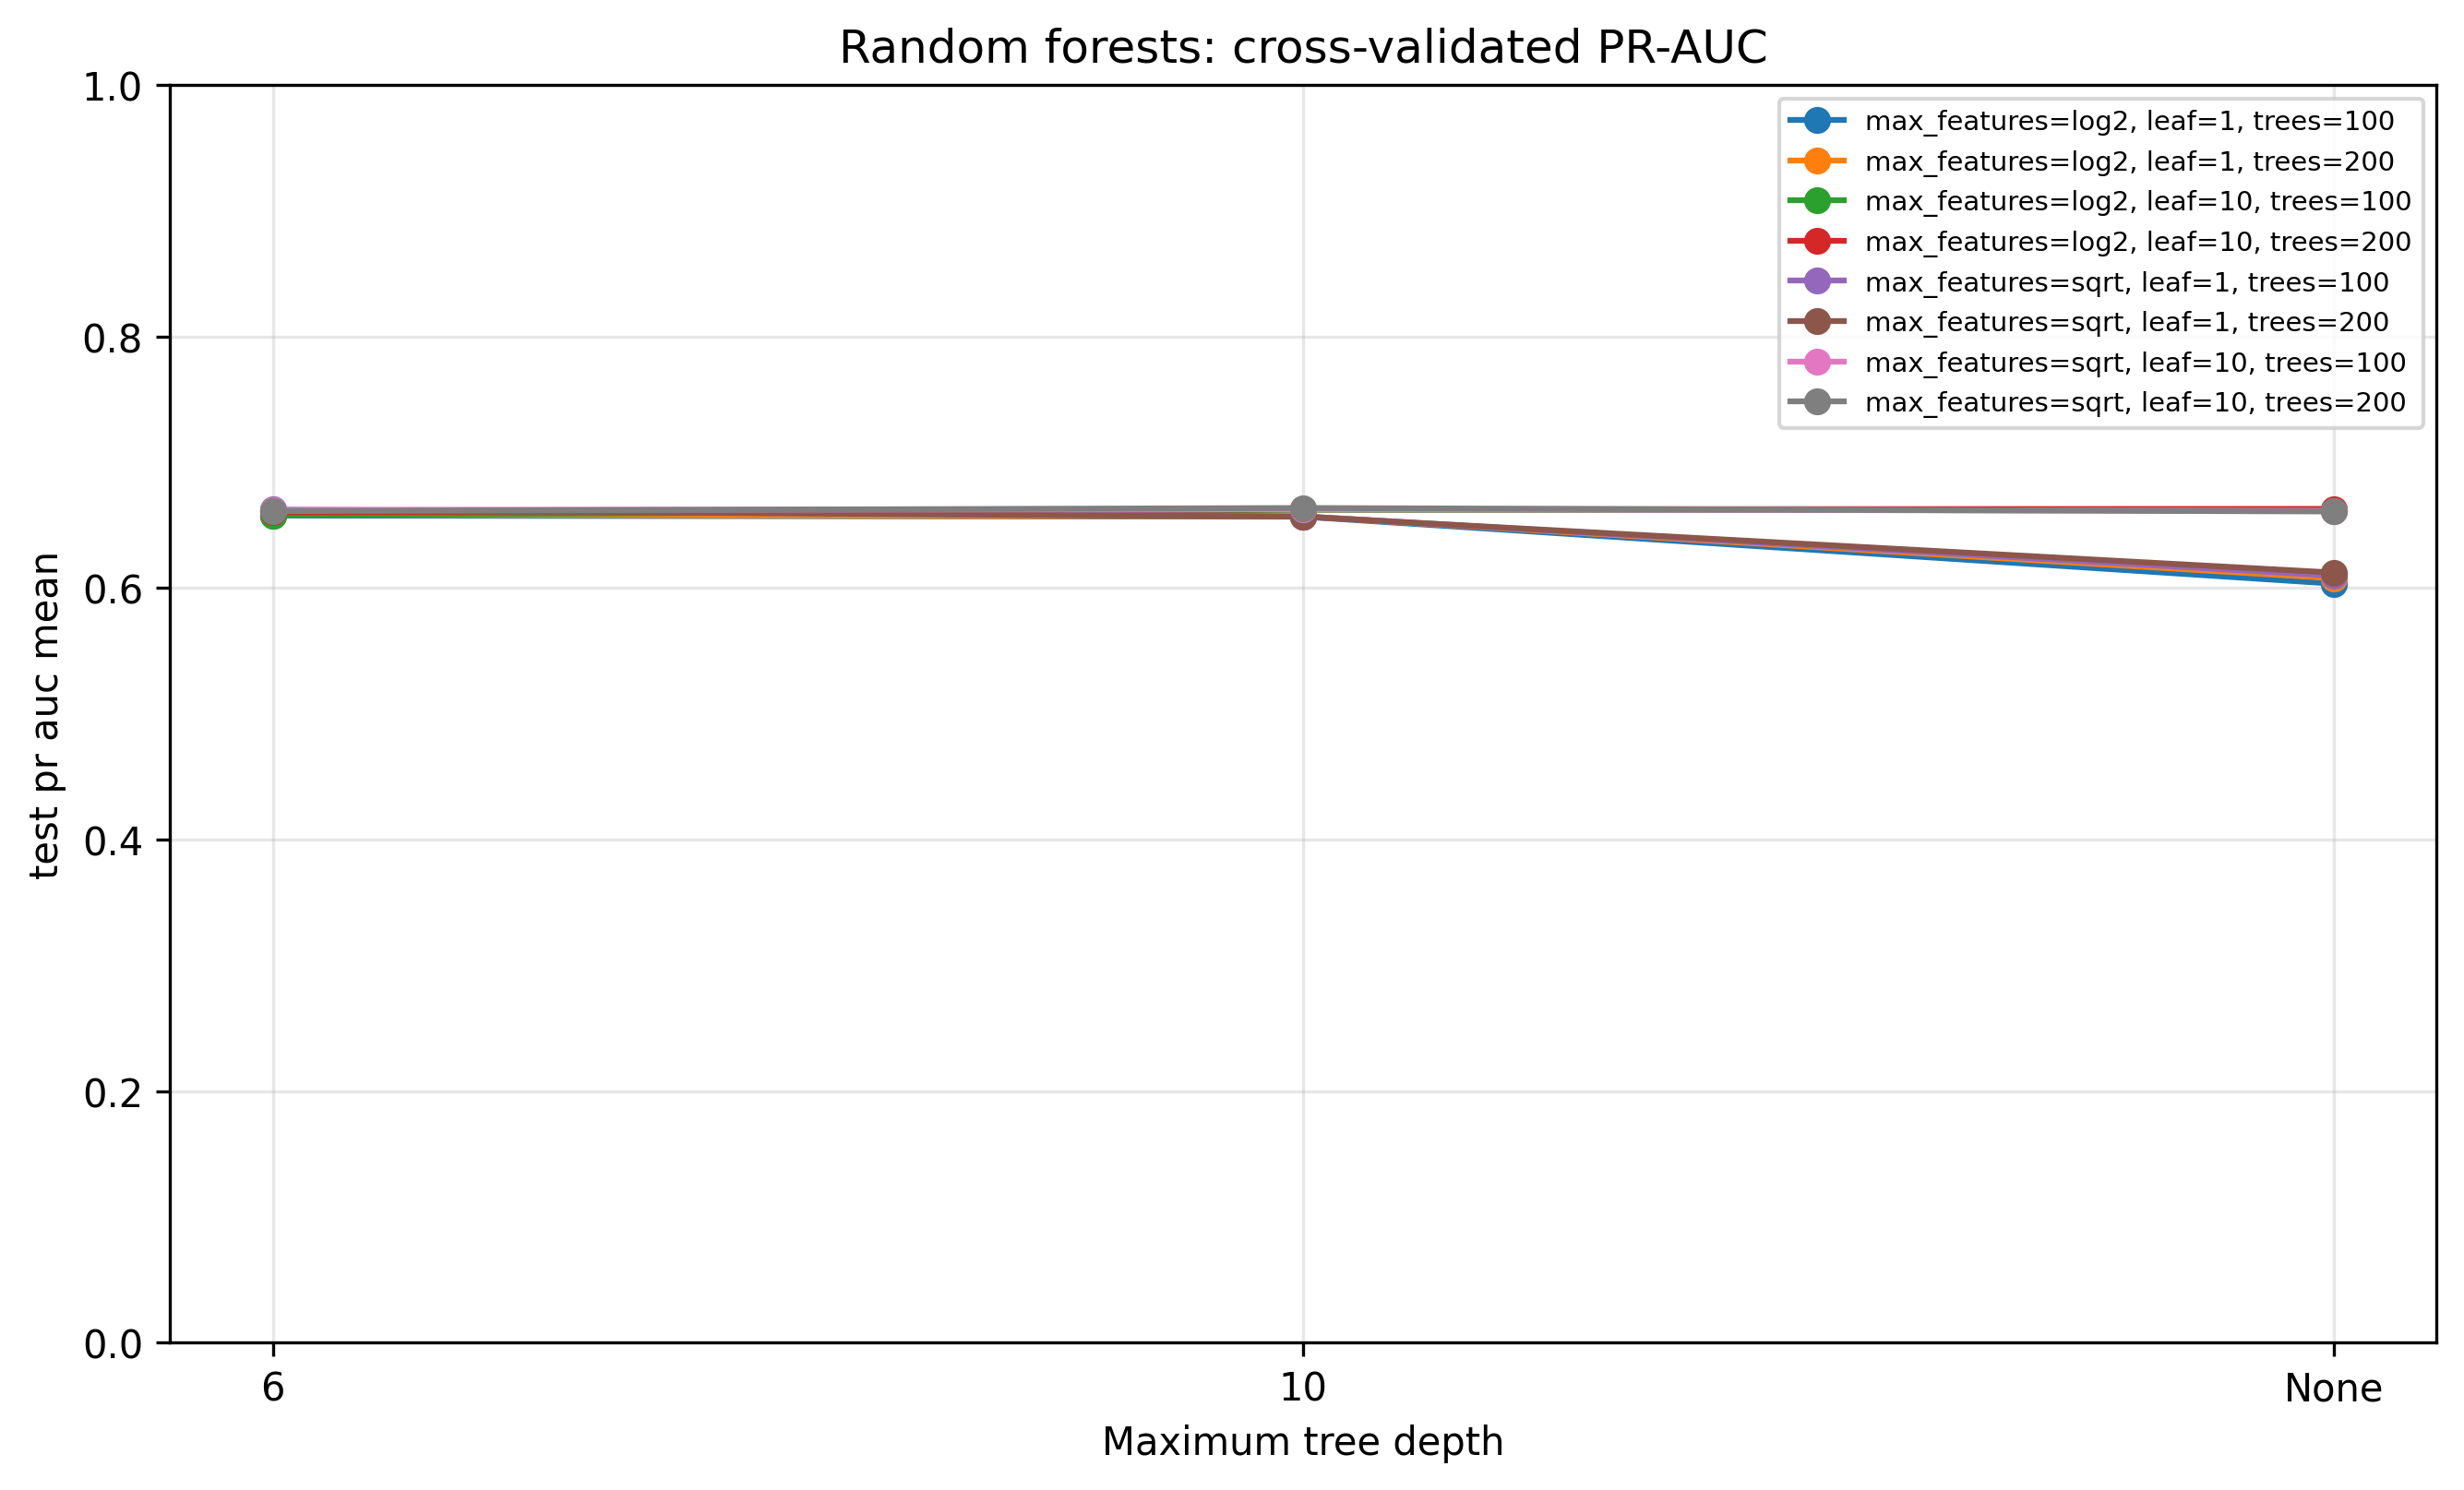
\includegraphics[width=0.88\textwidth]{../figures/random_forest_pr_auc_by_depth.png}
\caption{Random forests: cross-validated PR-AUC by maximum tree depth}
\label{fig:random-forest-pr-auc-by-depth}
\end{figure}

The unrestricted-depth random-forest settings are weaker by PR-AUC than the depth-6 and depth-10 settings. This is consistent with the general tree-regularization pattern already seen in Section~\ref{sec:decision-trees}: even inside an ensemble, overly flexible trees can add noisy splits that do not improve validation ranking performance.

Figure~\ref{fig:random-forest-balanced-accuracy-by-depth} shows the random-forest grid using balanced accuracy. The metric is again very stable across many configurations. The depth-10 settings are slightly stronger than depth 6 and unrestricted depth, but the differences are small.

\begin{figure}[H]
\centering
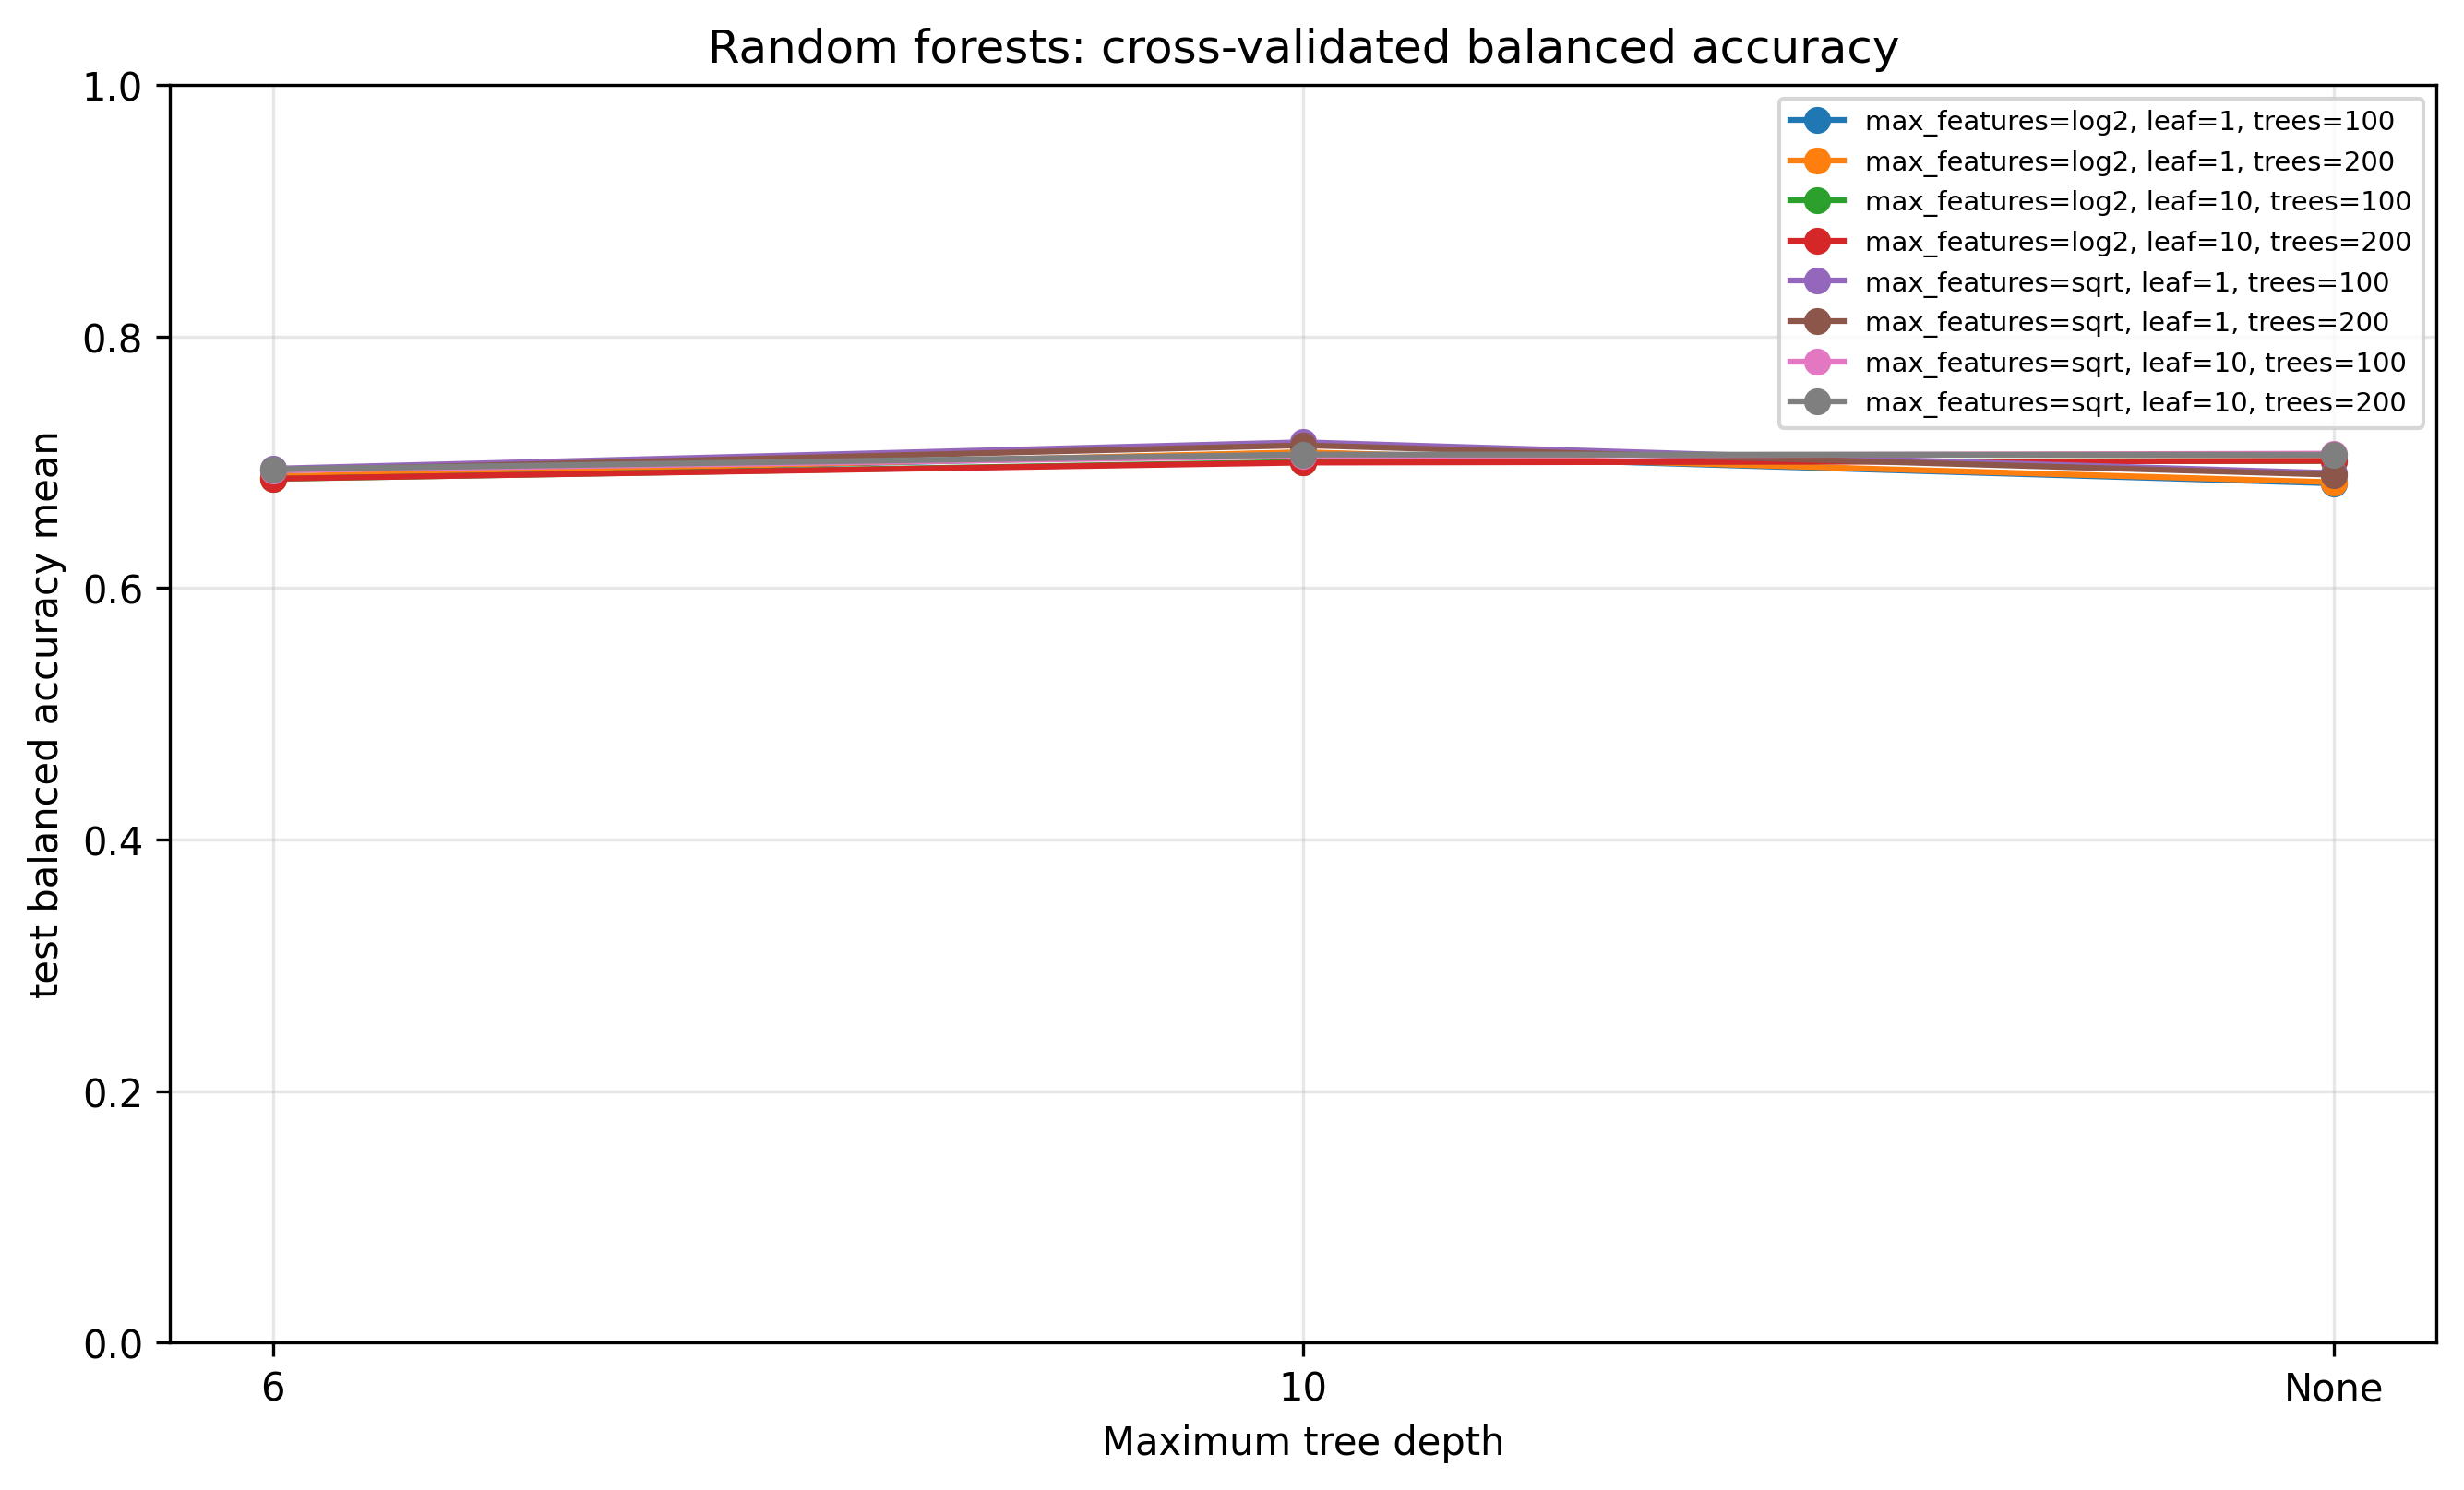
\includegraphics[width=0.88\textwidth]{../figures/random_forest_balanced_accuracy_by_depth.png}
\caption{Random forests: cross-validated balanced accuracy by maximum tree depth}
\label{fig:random-forest-balanced-accuracy-by-depth}
\end{figure}

\subsection{Model comparison}

Table~\ref{tab:bagging-random-forest-model-comparison} compares the selected tree-ensemble candidates with the selected single decision tree and a default random forest. The selected bagged-tree ensemble improves PR-AUC from approximately \(0.628\) for the single tree to approximately \(0.662\). The selected random forest obtains PR-AUC approximately \(0.660\). Both ensembles also improve ROC-AUC from approximately \(0.824\) to approximately \(0.846\) or \(0.847\).

\begin{table}[H]
\centering
\small
\resizebox{\textwidth}{!}{
\begin{tabular}{lrrrrrrrr}
\toprule
Model & Accuracy & Bal. Acc. & Precision & Recall & Specificity & \(F_1\) & ROC-AUC & PR-AUC \\
\midrule
Best bagged trees & 0.800 & 0.705 & 0.662 & 0.504 & 0.907 & 0.572 & 0.846 & 0.662 \\
Best random forest & 0.804 & 0.706 & 0.678 & 0.498 & 0.914 & 0.574 & 0.847 & 0.660 \\
Selected single decision tree & 0.789 & 0.701 & 0.624 & 0.514 & 0.888 & 0.564 & 0.824 & 0.628 \\
Default random forest, 100 estimators & 0.788 & 0.691 & 0.629 & 0.486 & 0.896 & 0.548 & 0.821 & 0.608 \\
\bottomrule
\end{tabular}
}
\caption{Cross-validated bagging and random-forest model comparison on the training set}
\label{tab:bagging-random-forest-model-comparison}
\end{table}

The main conclusion is not that plain bagging is statistically superior to random forests. The two selected ensemble variants are very close. Plain bagging has the slightly higher PR-AUC point estimate, while the random forest has slightly higher ROC-AUC, balanced accuracy, precision, specificity, and \(F_1\). These differences are too small to interpret as statistical evidence that one tree-ensemble variant is truly better. The stronger conclusion is that bagging-based ensembles clearly improve over the single decision tree.

The corresponding positive-first confusion-matrix counts are shown in Table~\ref{tab:bagging-random-forest-confusion}. At the default threshold, the selected bagged trees detect \(753\) of the \(1495\) churners and produce \(385\) false positives. The selected random forest detects \(744\) churners and produces \(354\) false positives. Thus, the selected random forest is slightly more conservative at the default threshold, with fewer positives flagged overall.

\begin{table}[H]
\centering
\small
\begin{tabular}{lrrrrr}
\toprule
Model & TP & FN & FP & TN & Pred. positive rate \\
\midrule
Best bagged trees & 753 & 742 & 385 & 3754 & 0.202 \\
Best random forest & 744 & 751 & 354 & 3785 & 0.195 \\
Selected single decision tree & 769 & 726 & 463 & 3676 & 0.219 \\
Default random forest, 100 estimators & 727 & 768 & 429 & 3710 & 0.205 \\
\bottomrule
\end{tabular}
\caption{Positive-first confusion-matrix counts for bagging and random forests}
\label{tab:bagging-random-forest-confusion}
\end{table}

\subsection{Out-of-bag diagnostics}

Table~\ref{tab:bagging-random-forest-oob} reports out-of-bag diagnostics for the selected ensemble candidates. The out-of-bag PR-AUC values are close to the cross-validated PR-AUC values, which is reassuring. The selected bagged-tree ensemble has out-of-bag PR-AUC approximately \(0.660\), while the selected random forest has out-of-bag PR-AUC approximately \(0.663\).

\begin{table}[H]
\centering
\small
\begin{tabular}{lrrrr}
\toprule
Model & OOB accuracy & OOB valid obs. & OOB ROC-AUC & OOB PR-AUC \\
\midrule
Best bagged trees & 0.801 & 5634 & 0.845 & 0.660 \\
Best random forest & 0.802 & 5634 & 0.847 & 0.663 \\
\bottomrule
\end{tabular}
\caption{Out-of-bag diagnostics for selected bagging-based ensembles}
\label{tab:bagging-random-forest-oob}
\end{table}

These out-of-bag diagnostics support the earlier caution about the bagging versus random-forest comparison. The fixed-grid CV PR-AUC point estimate is slightly higher for plain bagging, while the out-of-bag PR-AUC is slightly higher for the random forest. This does not create a contradiction. It shows that the two ensemble variants are close enough that small changes in evaluation procedure can change their ordering.

\subsection{Threshold behaviour}

Figure~\ref{fig:bagging-random-forest-threshold-tradeoff} shows the threshold tradeoff for the selected PR-AUC representative, the bagged-tree ensemble. Lower thresholds increase recall but reduce precision and specificity. Higher thresholds reduce the number of flagged customers, raising precision and specificity but lowering recall.

\begin{figure}[H]
\centering
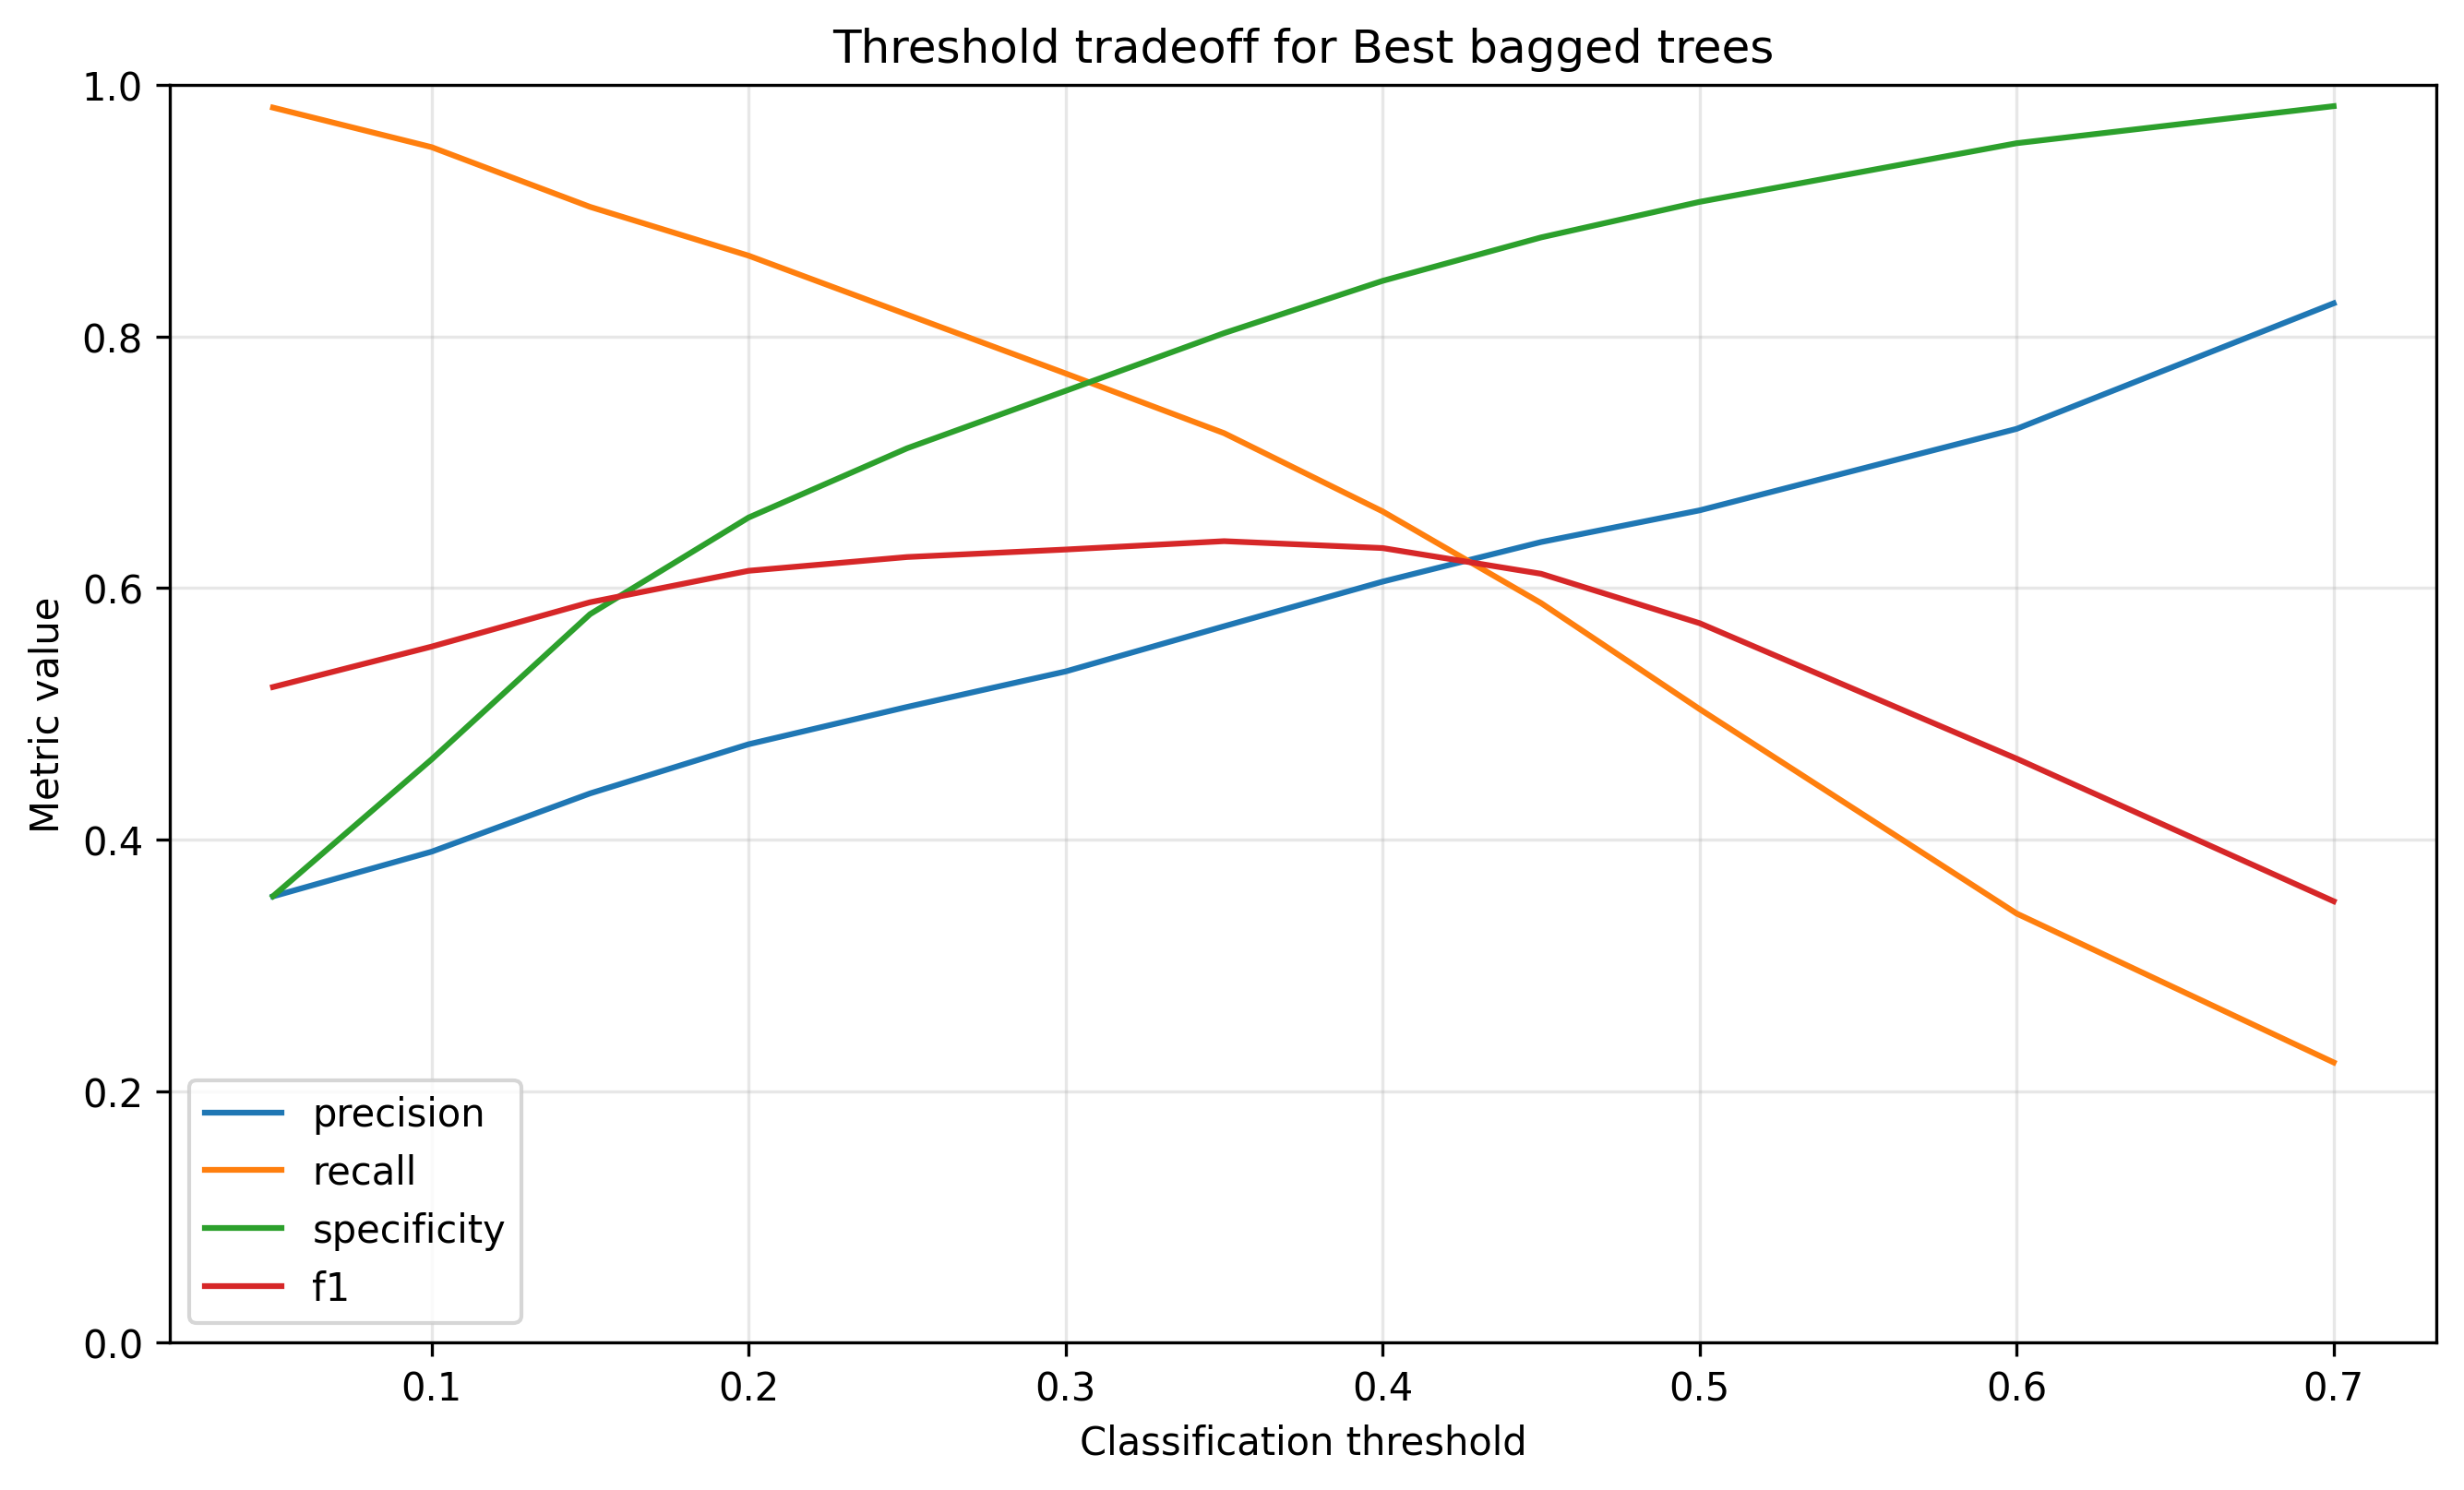
\includegraphics[width=0.88\textwidth]{../figures/bagging_random_forest_threshold_tradeoff.png}
\caption{Threshold tradeoff for the selected bagged-tree ensemble}
\label{fig:bagging-random-forest-threshold-tradeoff}
\end{figure}

At threshold \(0.30\), the selected bagged trees have recall approximately \(0.772\), precision approximately \(0.531\), specificity approximately \(0.762\), and \(F_1\) approximately \(0.629\). At threshold \(0.40\), recall is approximately \(0.665\), precision approximately \(0.604\), specificity approximately \(0.843\), and \(F_1\) approximately \(0.633\). At the default threshold \(0.50\), recall falls to approximately \(0.504\), while precision rises to approximately \(0.662\). This again confirms that threshold choice is a separate operating decision and should not be confused with model ranking performance.

\subsection{ROC and precision-recall curves}

Figure~\ref{fig:bagging-random-forest-roc-curve} shows the ROC curve for the selected bagged-tree ensemble. The ROC-AUC is approximately \(0.846\), which improves over the selected single decision tree.

\begin{figure}[H]
\centering
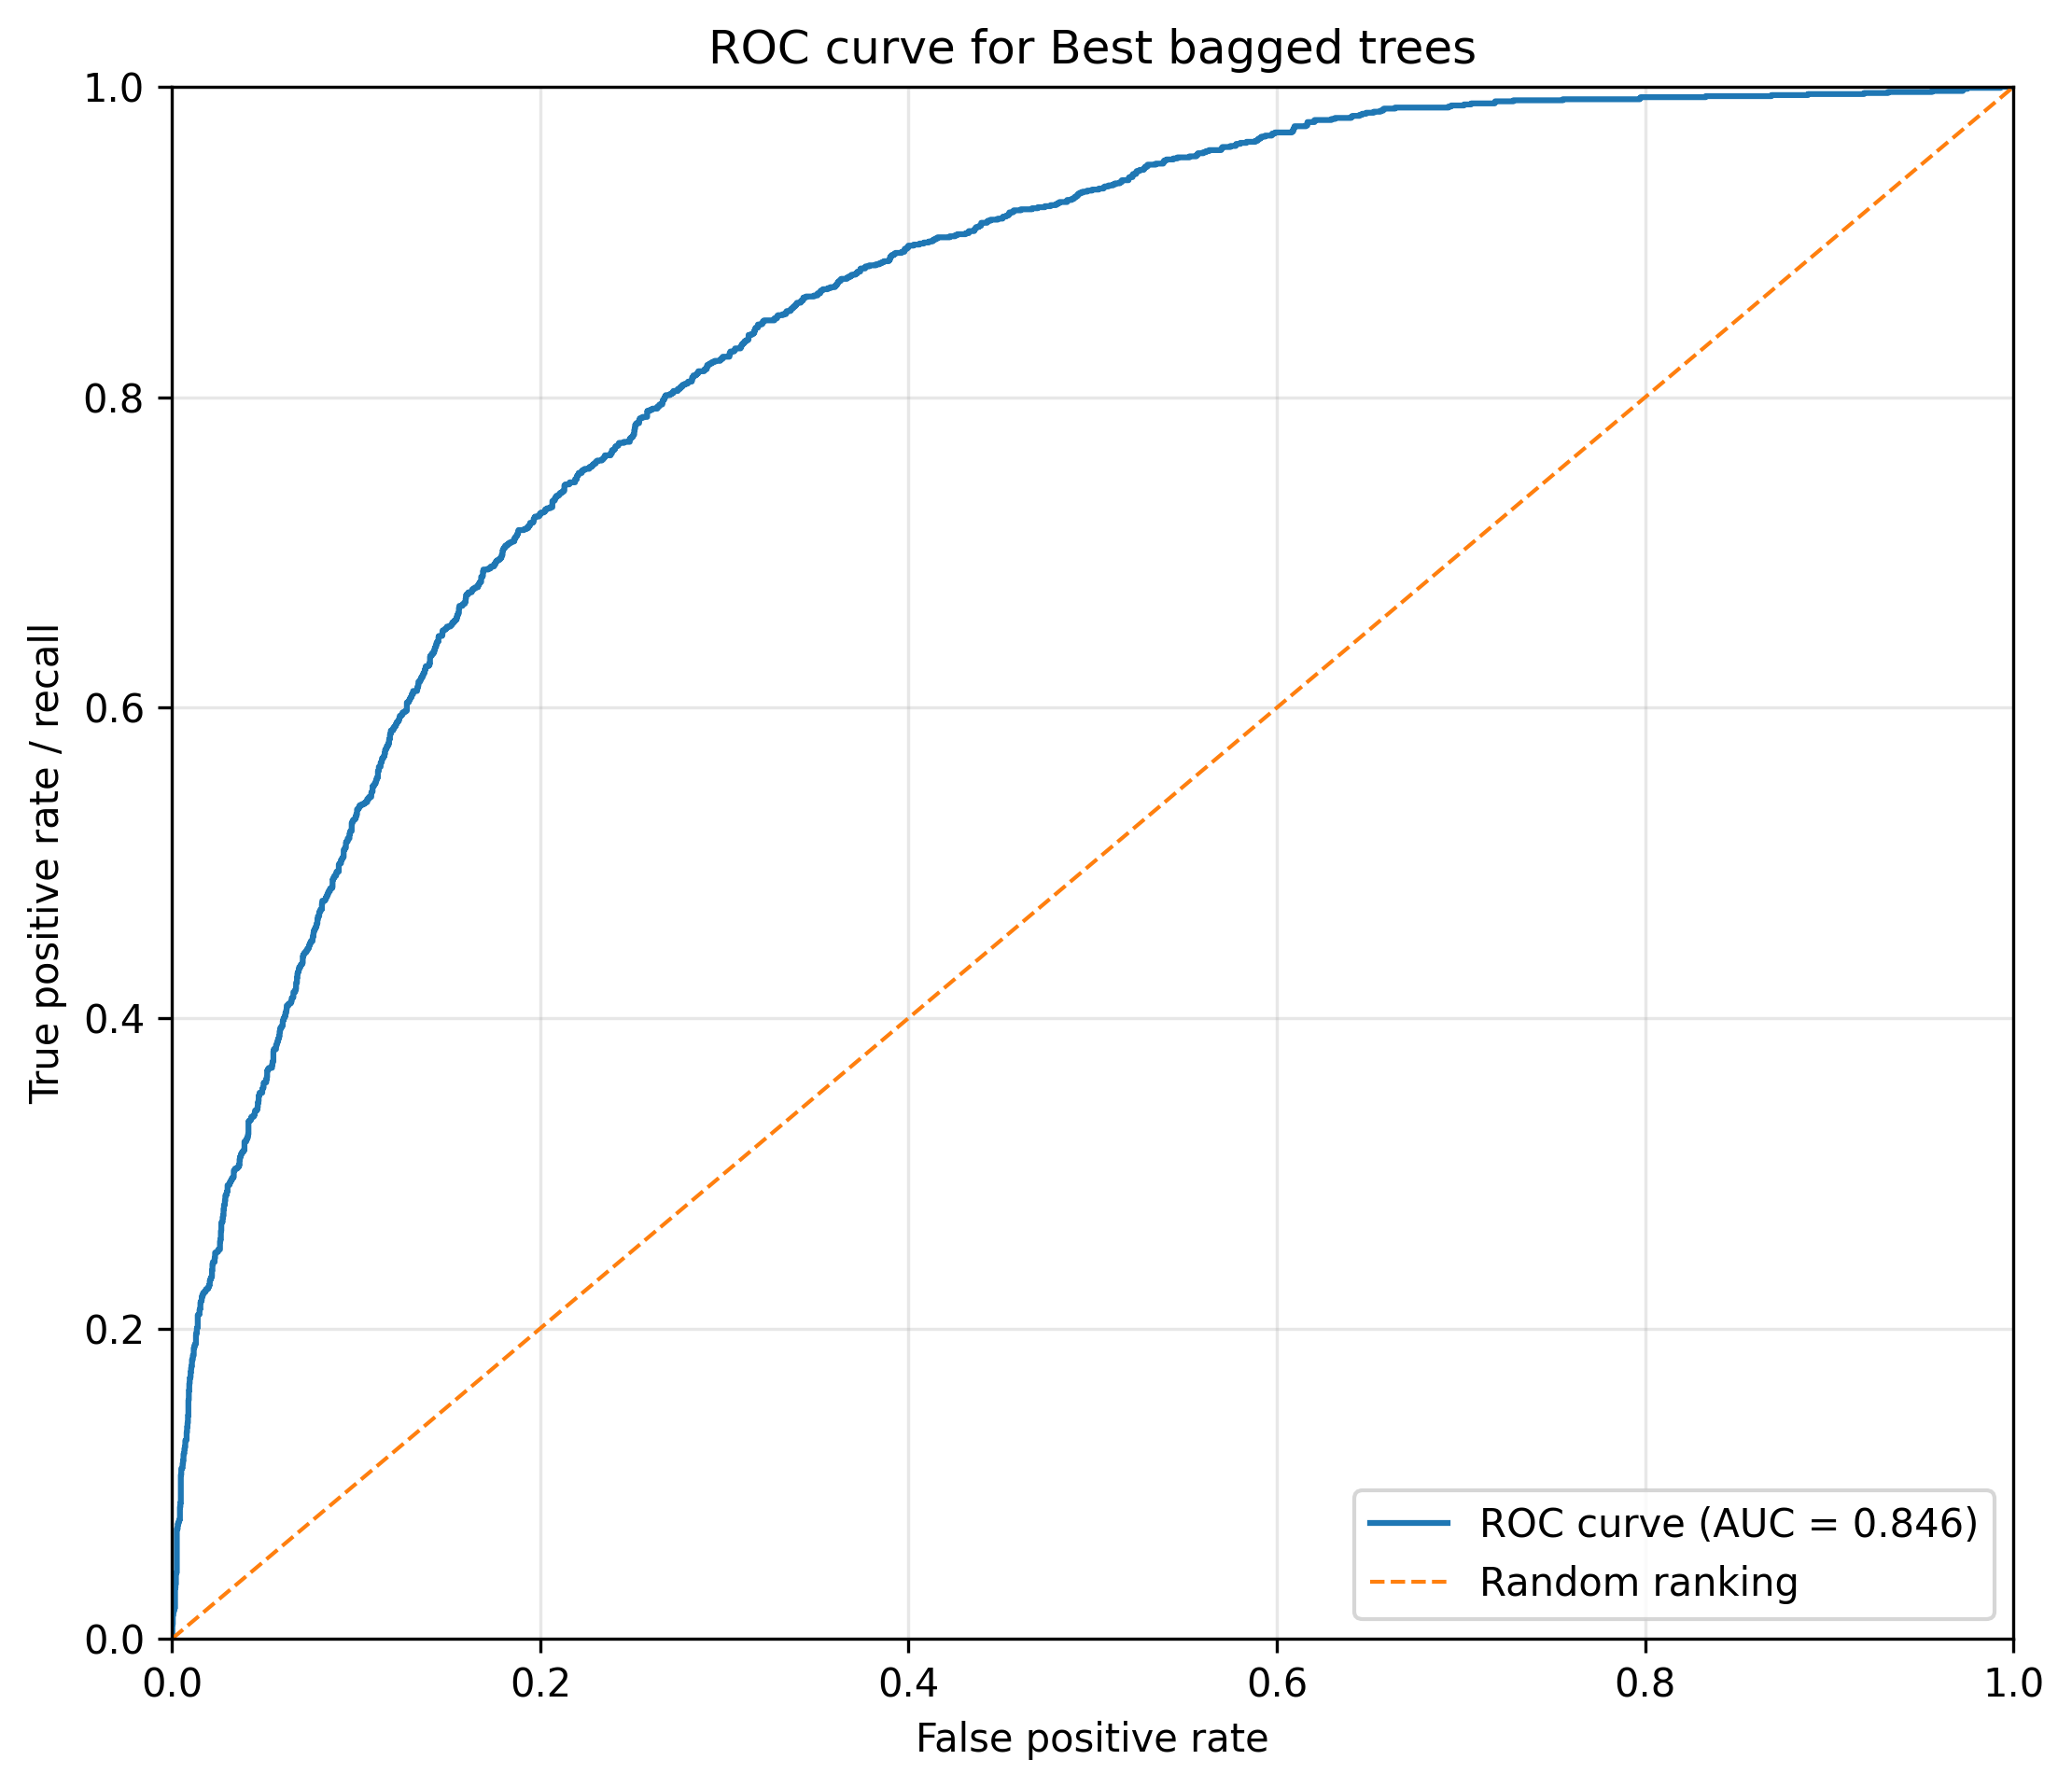
\includegraphics[width=0.88\textwidth]{../figures/bagging_random_forest_roc_curve.png}
\caption{ROC curve for the selected bagged-tree ensemble}
\label{fig:bagging-random-forest-roc-curve}
\end{figure}

Figure~\ref{fig:bagging-random-forest-pr-curve} shows the corresponding precision-recall curve. The PR-AUC is approximately \(0.661\), well above the positive-rate baseline of approximately \(0.265\). The curve shows that high precision is possible only for the highest-risk customers, while precision gradually decreases as recall approaches one.

\begin{figure}[H]
\centering
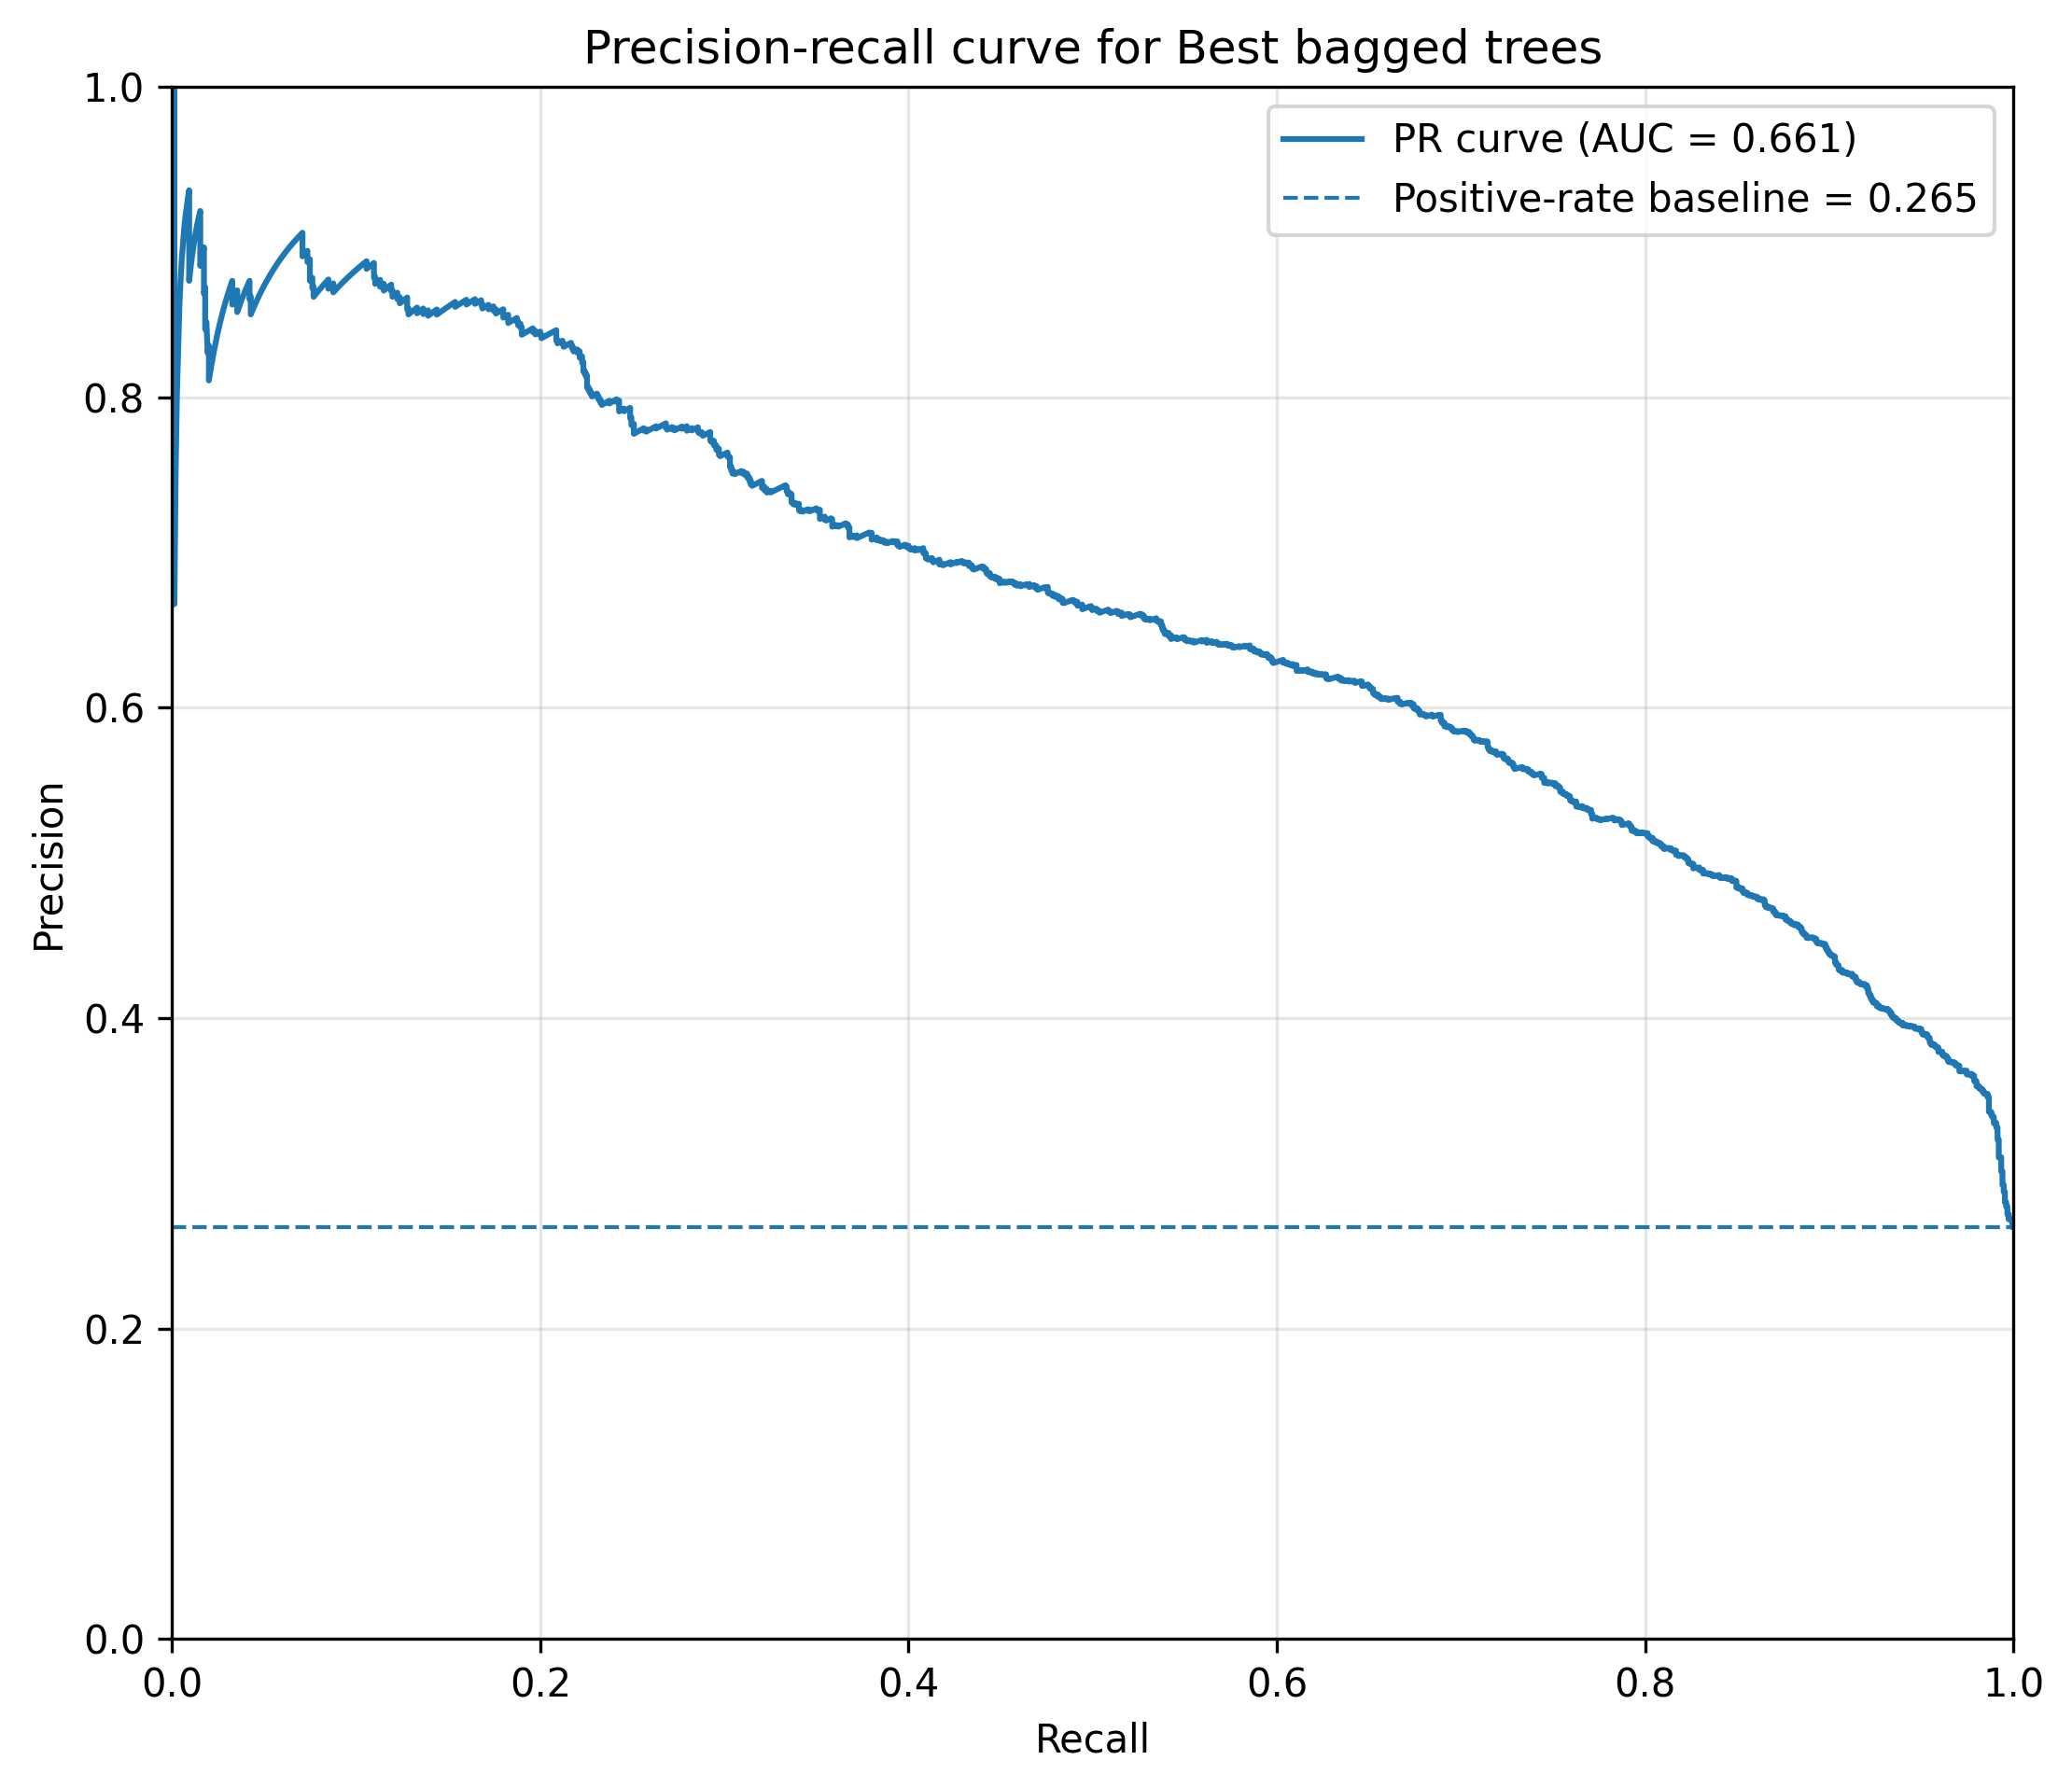
\includegraphics[width=0.88\textwidth]{../figures/bagging_random_forest_precision_recall_curve.png}
\caption{Precision-recall curve for the selected bagged-tree ensemble}
\label{fig:bagging-random-forest-pr-curve}
\end{figure}

\subsection{Random-forest feature importance}

Although the selected PR-AUC representative is the bagged-tree ensemble, the best random forest is retained as a close comparator and as a useful interpretation model. Figure~\ref{fig:random-forest-feature-importance} shows impurity-based feature importance for the best random forest.

\begin{figure}[H]
\centering
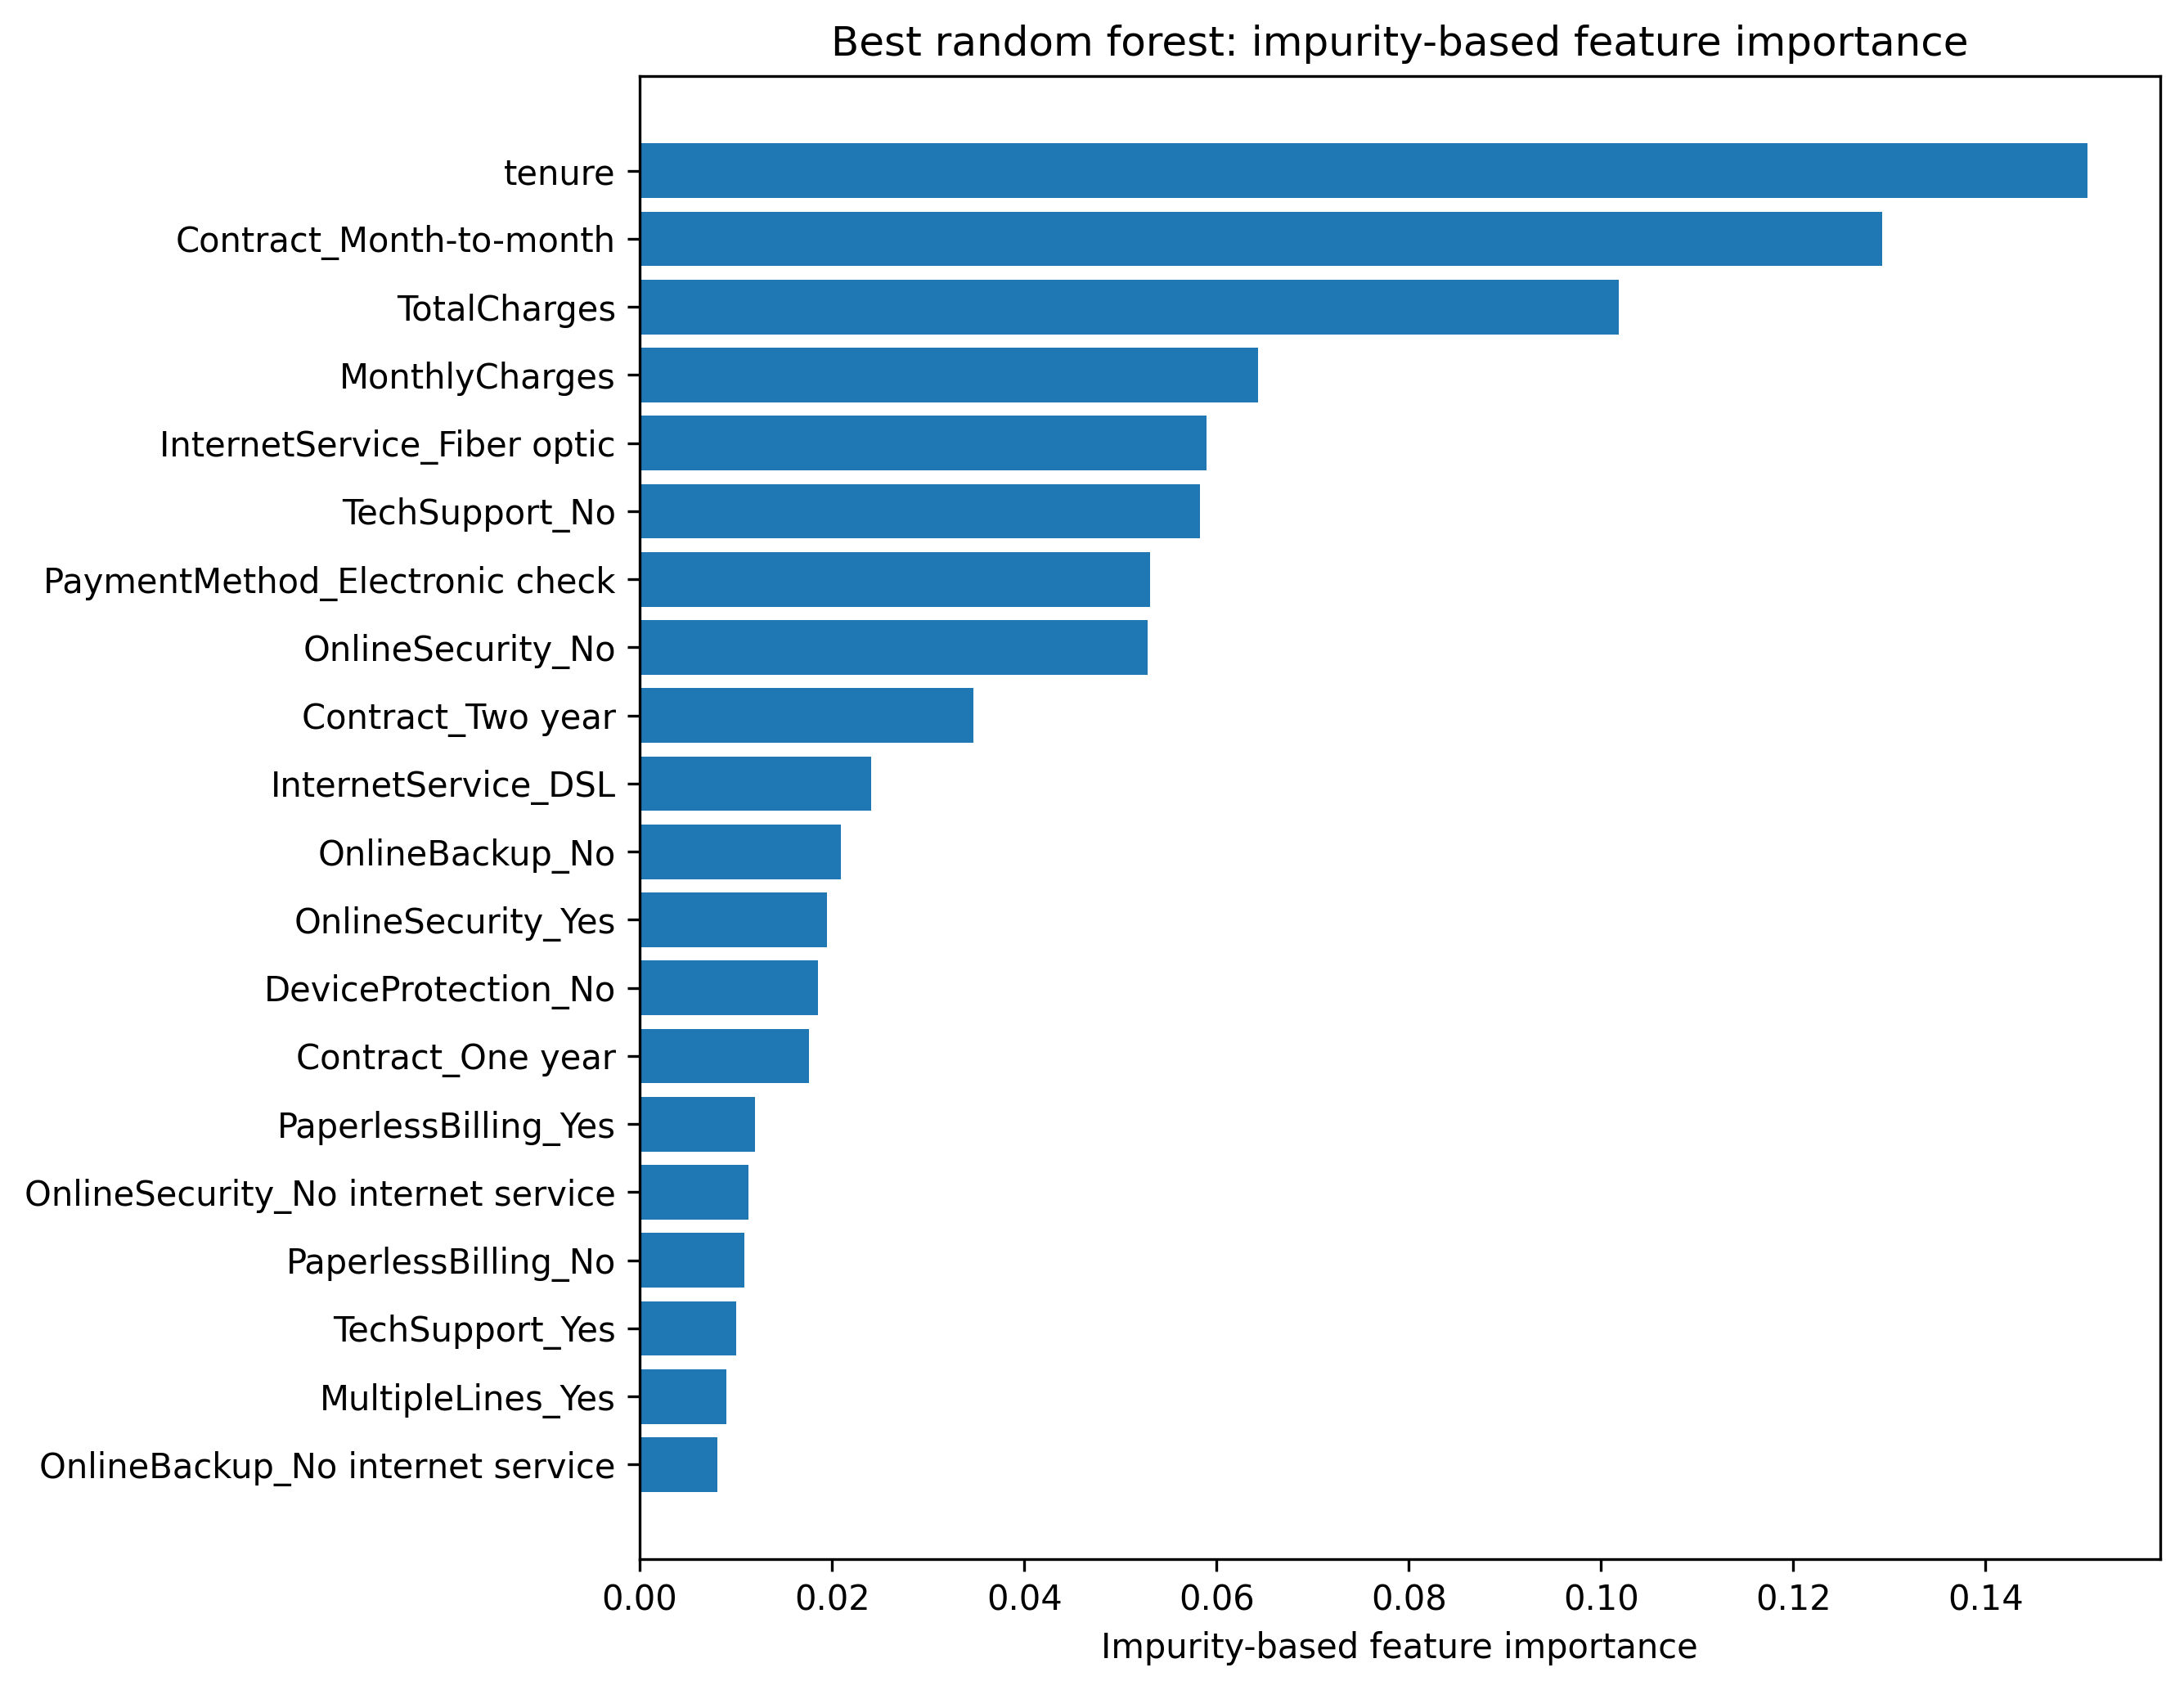
\includegraphics[width=0.88\textwidth]{../figures/random_forest_feature_importance.png}
\caption{Best random forest: impurity-based feature importance}
\label{fig:random-forest-feature-importance}
\end{figure}

The most important variables are tenure, month-to-month contract status, total charges, monthly charges, fibre-optic internet service, lack of technical support, electronic-check payment, and lack of online security. This agrees with the main churn patterns found in earlier sections: contract structure, customer tenure, service type, and billing/payment behaviour are central to churn risk.

The feature-importance values should still be interpreted cautiously. Impurity-based importance measures how much splits on a feature reduce tree impurity across the forest. It is not a causal effect and it can be affected by feature correlation and the number of possible split points. In this project, feature importance is used as a descriptive diagnostic rather than as causal evidence.

\subsection{Summary}

Bagging-based tree ensembles improve meaningfully over the selected single decision tree. The selected bagged-tree ensemble raises PR-AUC from approximately \(0.628\) to approximately \(0.662\), while the selected random forest obtains PR-AUC approximately \(0.660\). Both ensembles also improve ROC-AUC to approximately \(0.846\) or \(0.847\).

The comparison between plain bagging and random forests is close. Plain bagging has the highest development-stage PR-AUC in the fixed grid, but the random forest is slightly stronger on several secondary metrics and on the out-of-bag PR-AUC diagnostic. These small differences should not be interpreted as statistical proof that one variant is superior. The appropriate conclusion is that both variants are promising tree-ensemble candidates.

This section therefore adds an important modelling step to the project. A single decision tree is interpretable but unstable. Bagging and random forests reduce that instability by averaging many trees. The next modelling section will move from averaging trees to boosting, where trees are fitted sequentially so that later learners focus on mistakes made by earlier learners.


\newpage
\newpage
\section[Boosting, Gradient Boosting, and Modern Boosted Tree Libraries]{Boosting, Gradient Boosting, and Modern Boosted Tree \mbox{Libraries}}
\label{sec:boosting}

This section evaluates boosting models for churn prediction. The previous section studied bagging and random forests, where many trees are fitted independently and their predictions are averaged. Boosting changes the ensemble construction principle. Instead of fitting all base learners independently, boosting builds an additive model sequentially. Each new learner is fitted after the current ensemble has revealed errors, residuals, or gradient signals.

The same development discipline is used as in all previous modelling sections. The held-out test set is not used. All results are based on stratified cross-validation inside the training set. Fixed grids are used deliberately for model-family learning and transparent development-stage comparison. The selected rows are therefore the strongest candidates within the tried grids, not final globally optimized hyperparameters and not final test-set performance claims.

\subsection{From independent averaging to sequential correction}

Bagging-based ensembles average many independently fitted predictors. If tree \(b\) produces a churn-risk score \(\widehat{p}_b(x)\), a bagged ensemble predicts by averaging
\[
\widehat{p}_{\mathrm{bag}}(x)
=
\frac{1}{B}\sum_{b=1}^{B}\widehat{p}_b(x).
\]
The main statistical idea is variance reduction. A single tree can be unstable, and averaging many bootstrapped trees reduces that instability.

Boosting instead constructs an additive score. A generic boosted model can be written as
\[
F_T(x)
=
F_0(x)
+
\sum_{t=1}^{T}\nu_t h_t(x),
\]
where \(F_0\) is an initial score, \(h_t\) is the learner added at stage \(t\), and \(\nu_t\) is its contribution or shrinkage-adjusted weight. In binary classification, the score is often transformed into a probability through a logistic mapping,
\[
\widehat{p}(x)
=
\frac{1}{1+\exp(-F_T(x))}.
\]
The hard classification at threshold \(c\) is then
\[
\widehat{y}(x;c)=\mathbb{1}\{\widehat{p}(x)\geq c\}.
\]
Thus, boosting still produces ranking scores and threshold-dependent classifications. PR-AUC and ROC-AUC evaluate ranking quality, while precision, recall, specificity, and \(F_1\) depend on the chosen classification threshold.

\subsection{AdaBoost}

AdaBoost is the classical boosting algorithm for classification. It starts with observation weights and repeatedly fits weak learners. After each stage, observations that are misclassified receive more weight, so the next learner focuses more strongly on difficult cases.

For binary labels \(y_i\in\{-1,+1\}\), suppose learner \(h_t\) is fitted at stage \(t\). Its weighted error is
\[
\varepsilon_t
=
\frac{\sum_{i=1}^{n} w_i^{(t)}\mathbb{1}\{y_i\neq h_t(x_i)\}}
{\sum_{i=1}^{n} w_i^{(t)}}.
\]
The learner receives weight
\[
\alpha_t
=
\frac{1}{2}\log\left(\frac{1-\varepsilon_t}{\varepsilon_t}\right),
\]
and the observation weights are updated by
\[
w_i^{(t+1)}
\propto
w_i^{(t)}\exp\{-\alpha_t y_i h_t(x_i)\}.
\]
Misclassified observations have \(y_i h_t(x_i)=-1\), so their weights increase relative to correctly classified observations. The final classifier is a weighted vote across the weak learners,
\[
H(x)=\operatorname{sign}\left(\sum_{t=1}^{T}\alpha_t h_t(x)\right).
\]

In this project, AdaBoost is evaluated with shallow decision trees. Stumps and shallow trees are natural base learners because boosting is designed to combine weak learners into a stronger additive classifier. The main tuning parameters are the number of boosting rounds, the learning rate, and the base-tree depth.

\subsection{Gradient boosting}

Gradient boosting generalizes the boosting idea to differentiable loss functions. The model is still additive, but each new learner is fitted to the negative gradient of the loss with respect to the current model score.

Let \(\ell(y,F(x))\) be a differentiable loss. At stage \(t\), the pseudo-residual for observation \(i\) is
\[
r_{it}
=
-
\left[
\frac{\partial \ell(y_i,F(x_i))}{\partial F(x_i)}
\right]_{F=F_{t-1}}.
\]
A regression tree is then fitted to these pseudo-residuals. For squared-error regression, the negative gradient is the ordinary residual. For binary log loss with labels \(y_i\in\{0,1\}\), if \(p_i\) is the current predicted probability, the negative-gradient signal is
\[
y_i-p_i.
\]
Therefore, a gradient-boosted classification tree is not fitted directly to class labels through Gini or entropy in the same way as a standalone classification tree. Its tree structure is fitted to gradient-like targets that describe how the current additive score should change.

After the terminal regions are formed, each leaf receives a numeric output. For first-order intuition, the leaf output can be understood as an average pseudo-residual. For log loss and modern boosted tree implementations, leaf values are often adjusted by curvature information. If \(g_i\) is the ordinary gradient, \(h_i\) is the Hessian, and
\[
G_j=\sum_{i\in R_j}g_i,
\qquad
H_j=\sum_{i\in R_j}h_i,
\]
then a common Newton-style leaf output is
\[
w_j^*
=
-
\frac{G_j}{H_j+\lambda},
\]
where \(\lambda\) is an L2-style leaf regularization parameter. This expression explains why modern gradient boosting is often described as second-order boosting: both slope and curvature information can influence split evaluation and leaf outputs.

\subsection{Modern gradient-boosted tree implementations}

This section evaluates six boosting families.

\begin{itemize}[leftmargin=*]
    \item \textbf{AdaBoost}: classical reweighting-based boosting with shallow decision-tree base learners.
    \item \textbf{GradientBoostingClassifier}: scikit-learn's classical stagewise gradient boosting implementation.
    \item \textbf{HistGradientBoostingClassifier}: scikit-learn's histogram-based gradient boosting implementation, with binned split search and explicit L2-style regularization.
    \item \textbf{XGBoost}: a regularized second-order boosted-tree implementation evaluated on the dense one-hot representation.
    \item \textbf{LightGBM}: a histogram-based boosted-tree implementation evaluated with native categorical handling.
    \item \textbf{CatBoost}: a boosted-tree implementation evaluated with native categorical handling and ordered categorical processing.
\end{itemize}

XGBoost, LightGBM, and CatBoost are not fundamentally separate from gradient boosting. They are specialized, highly engineered implementations of boosted decision trees. The differences are in objective regularization, split search, tree-growth strategy, categorical-feature handling, and computational efficiency. XGBoost makes the regularized second-order objective and split-gain calculation explicit. LightGBM emphasizes histogram-based training, leaf-wise growth, gradient-based sampling ideas, feature bundling, and native categorical split support. CatBoost emphasizes ordered target-statistic transformations, ordered boosting logic, and symmetric tree structures.

\subsection{Experimental design}

All grids are evaluated with the same stratified cross-validation framework. PR-AUC remains the primary ranking metric because churn is the positive minority class. ROC-AUC, balanced accuracy, precision, recall, specificity, and \(F_1\) are retained as secondary diagnostics.

The notebook compares the selected boosting candidates against reference models from earlier sections:

\begin{itemize}[leftmargin=*]
    \item selected L2 logistic regression;
    \item selected single decision tree;
    \item selected bagged trees;
    \item selected random forest.
\end{itemize}

The one-hot branch is used for scikit-learn boosting and XGBoost. The native-categorical branch is used for LightGBM and CatBoost. This allows the notebook to compare both the standard one-hot representation used in previous sections and the categorical handling provided by modern gradient-boosted tree libraries.

\subsection{Fixed-grid family selection}

Table~\ref{tab:boosting-selection-summary} summarizes the strongest row from each boosting family according to mean cross-validated PR-AUC. CatBoost has the highest grid-level mean PR-AUC at approximately \(0.673\), followed very closely by scikit-learn's \texttt{GradientBoostingClassifier} and XGBoost, both also around \(0.672\). LightGBM, AdaBoost, and \texttt{HistGradientBoostingClassifier} are slightly lower in this fixed-grid comparison.

\begin{table}[H]
\centering
\small
\begin{tabular}{lrrrrr}
\toprule
Family & PR-AUC & ROC-AUC & Bal. Acc. & \(F_1\) & Train PR-AUC \\
\midrule
CatBoost & 0.673 & 0.850 & 0.717 & 0.591 & 0.693 \\
GradientBoosting & 0.672 & 0.851 & 0.719 & 0.595 & 0.726 \\
XGBoost & 0.672 & 0.850 & 0.722 & 0.598 & 0.700 \\
LightGBM & 0.669 & 0.850 & 0.711 & 0.581 & 0.731 \\
AdaBoost & 0.665 & 0.848 & 0.718 & 0.592 & 0.682 \\
HistGradientBoosting & 0.665 & 0.849 & 0.719 & 0.593 & 0.764 \\
\bottomrule
\end{tabular}
\caption{Best fixed-grid candidate from each boosting family by mean cross-validated PR-AUC}
\label{tab:boosting-selection-summary}
\end{table}

The table should be interpreted cautiously. The top three values differ only in the third decimal place. The family ordering is useful development-stage evidence, but it is not a statistical proof that CatBoost, GradientBoosting, or XGBoost is truly superior. It also shows why final model comparison should be separated from model-family learning: once models are this close, repeated cross-validation, paired comparisons, or a more formal final training-only comparison procedure become more relevant.

Figures~\ref{fig:adaboost-pr-auc-grid} to~\ref{fig:catboost-pr-auc-grid} show the top PR-AUC candidates within each grid. The plots make the same point visually: many neighbouring configurations are close, especially for the modern boosted tree libraries.

\begin{figure}[H]
\centering
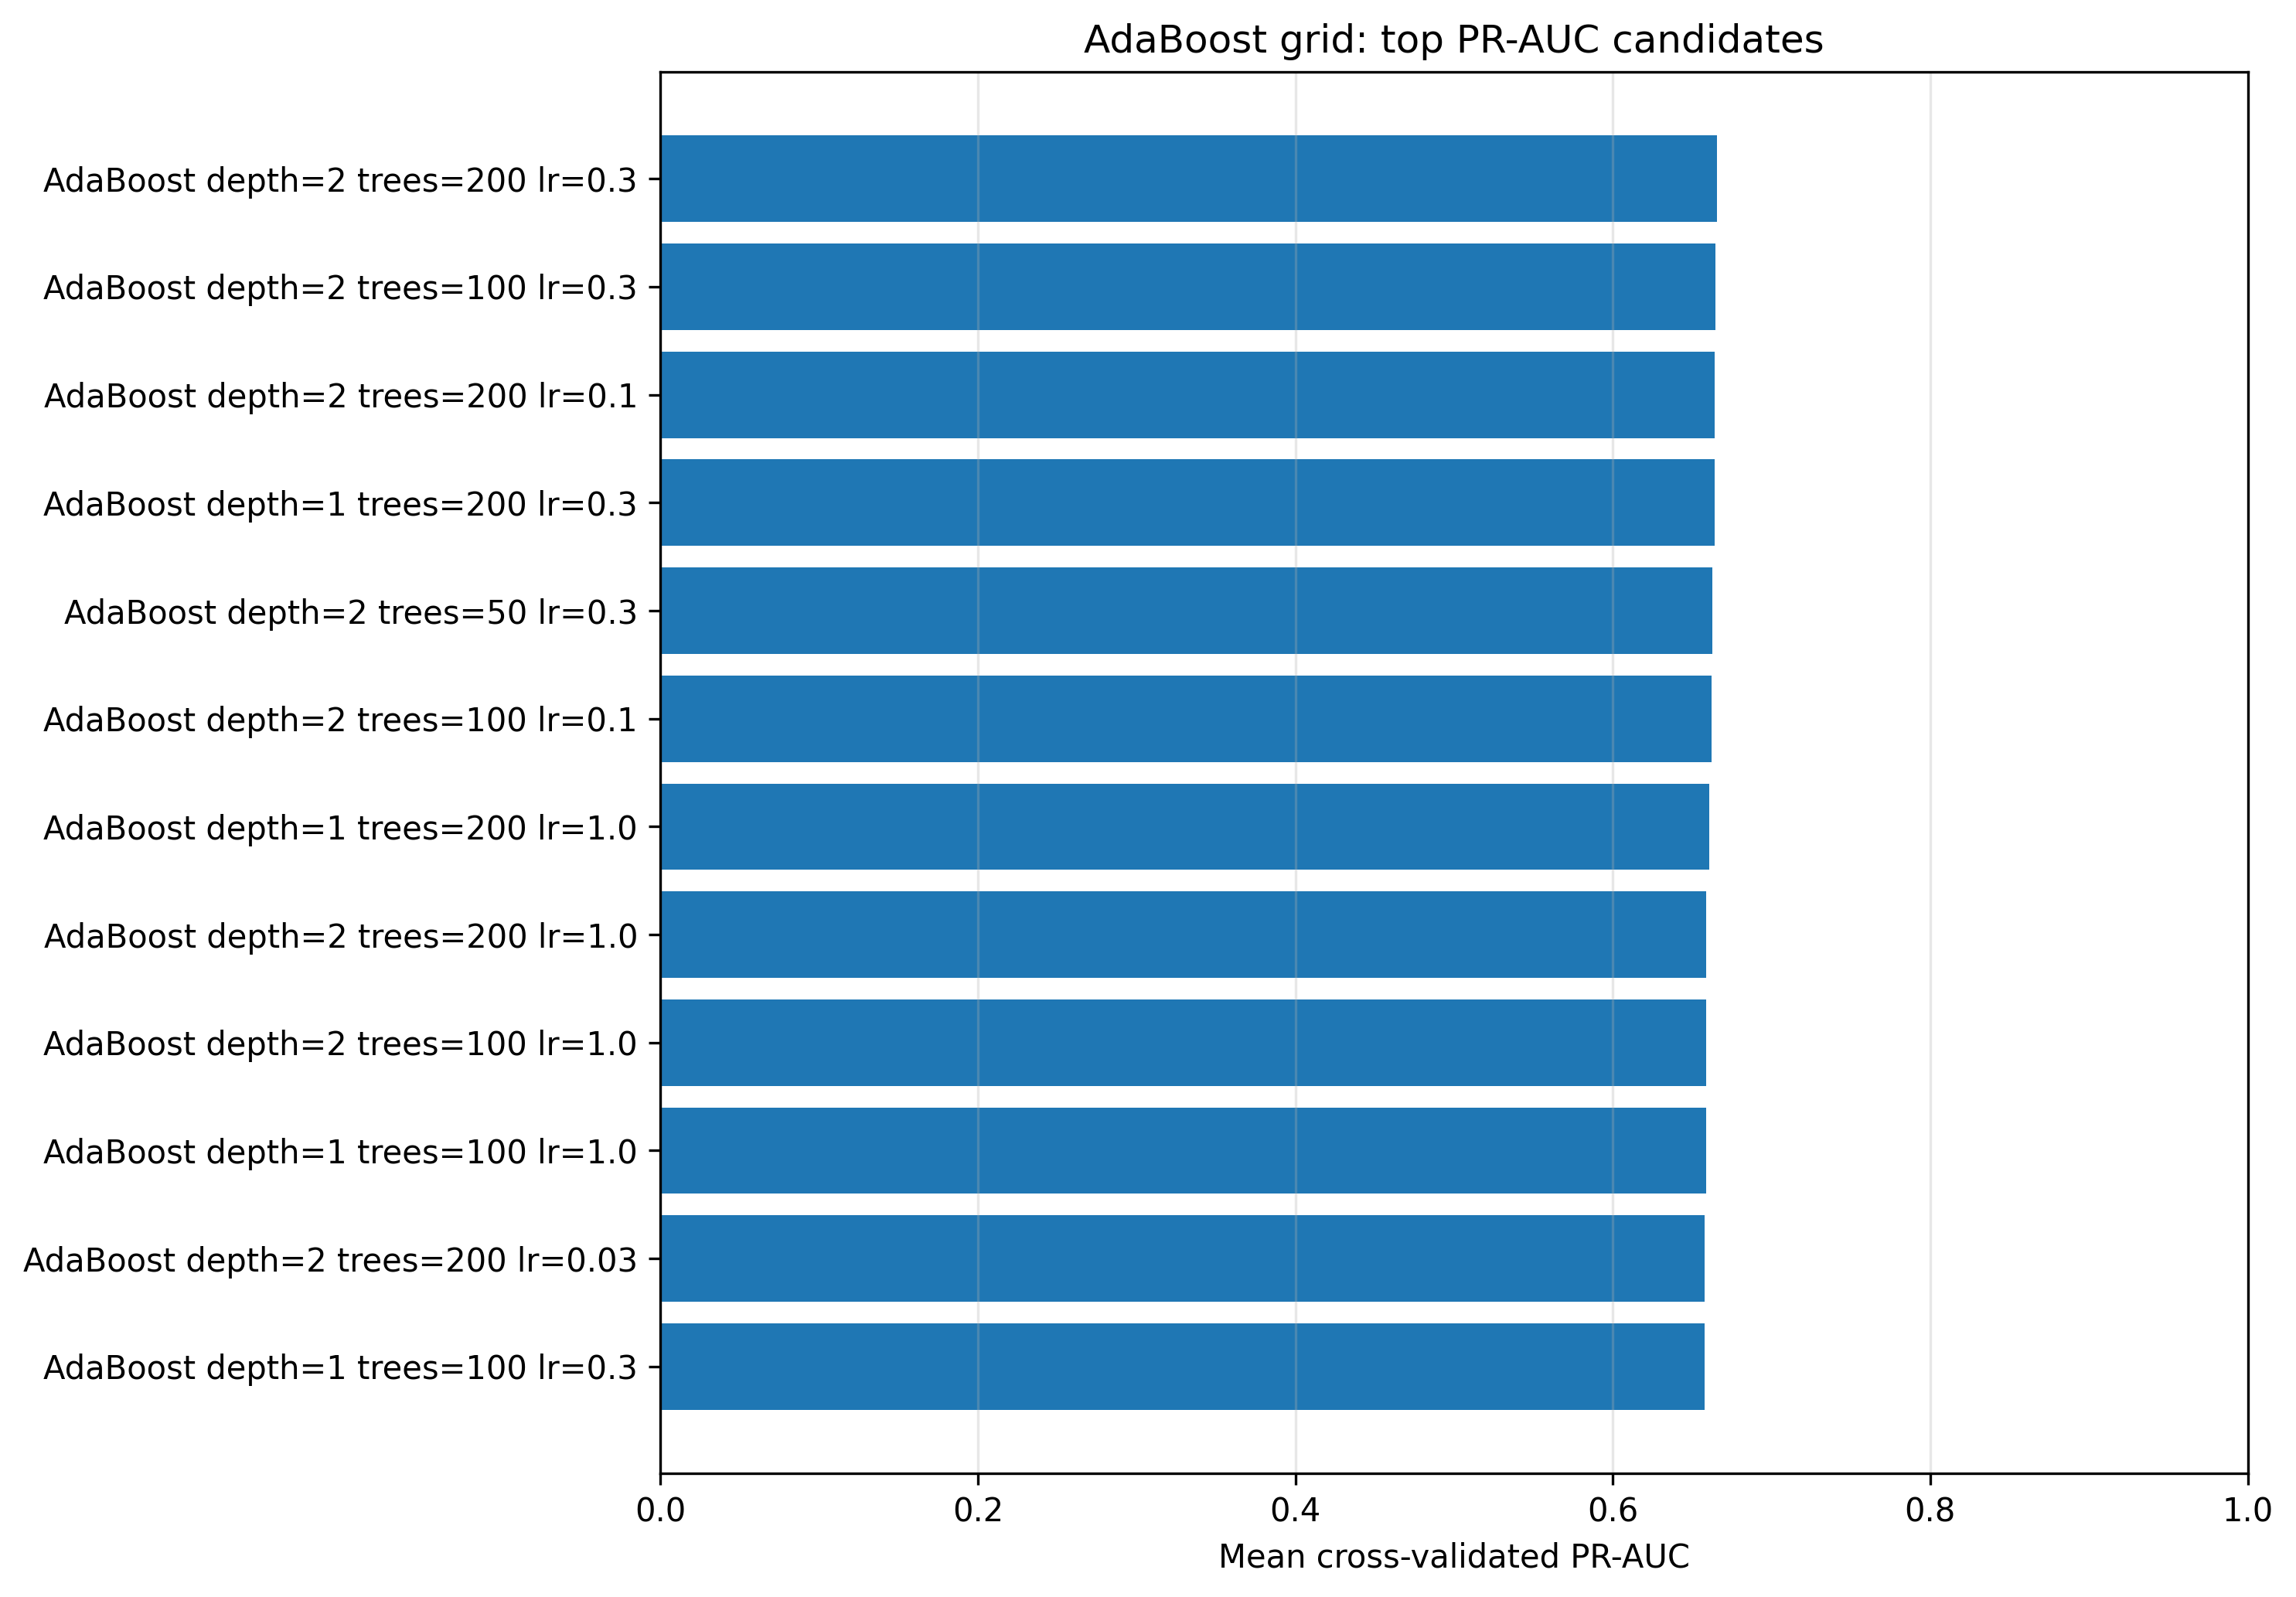
\includegraphics[width=0.88\textwidth]{../figures/adaboost_pr_auc_grid.png}
\caption{AdaBoost grid: top cross-validated PR-AUC candidates}
\label{fig:adaboost-pr-auc-grid}
\end{figure}

\begin{figure}[H]
\centering
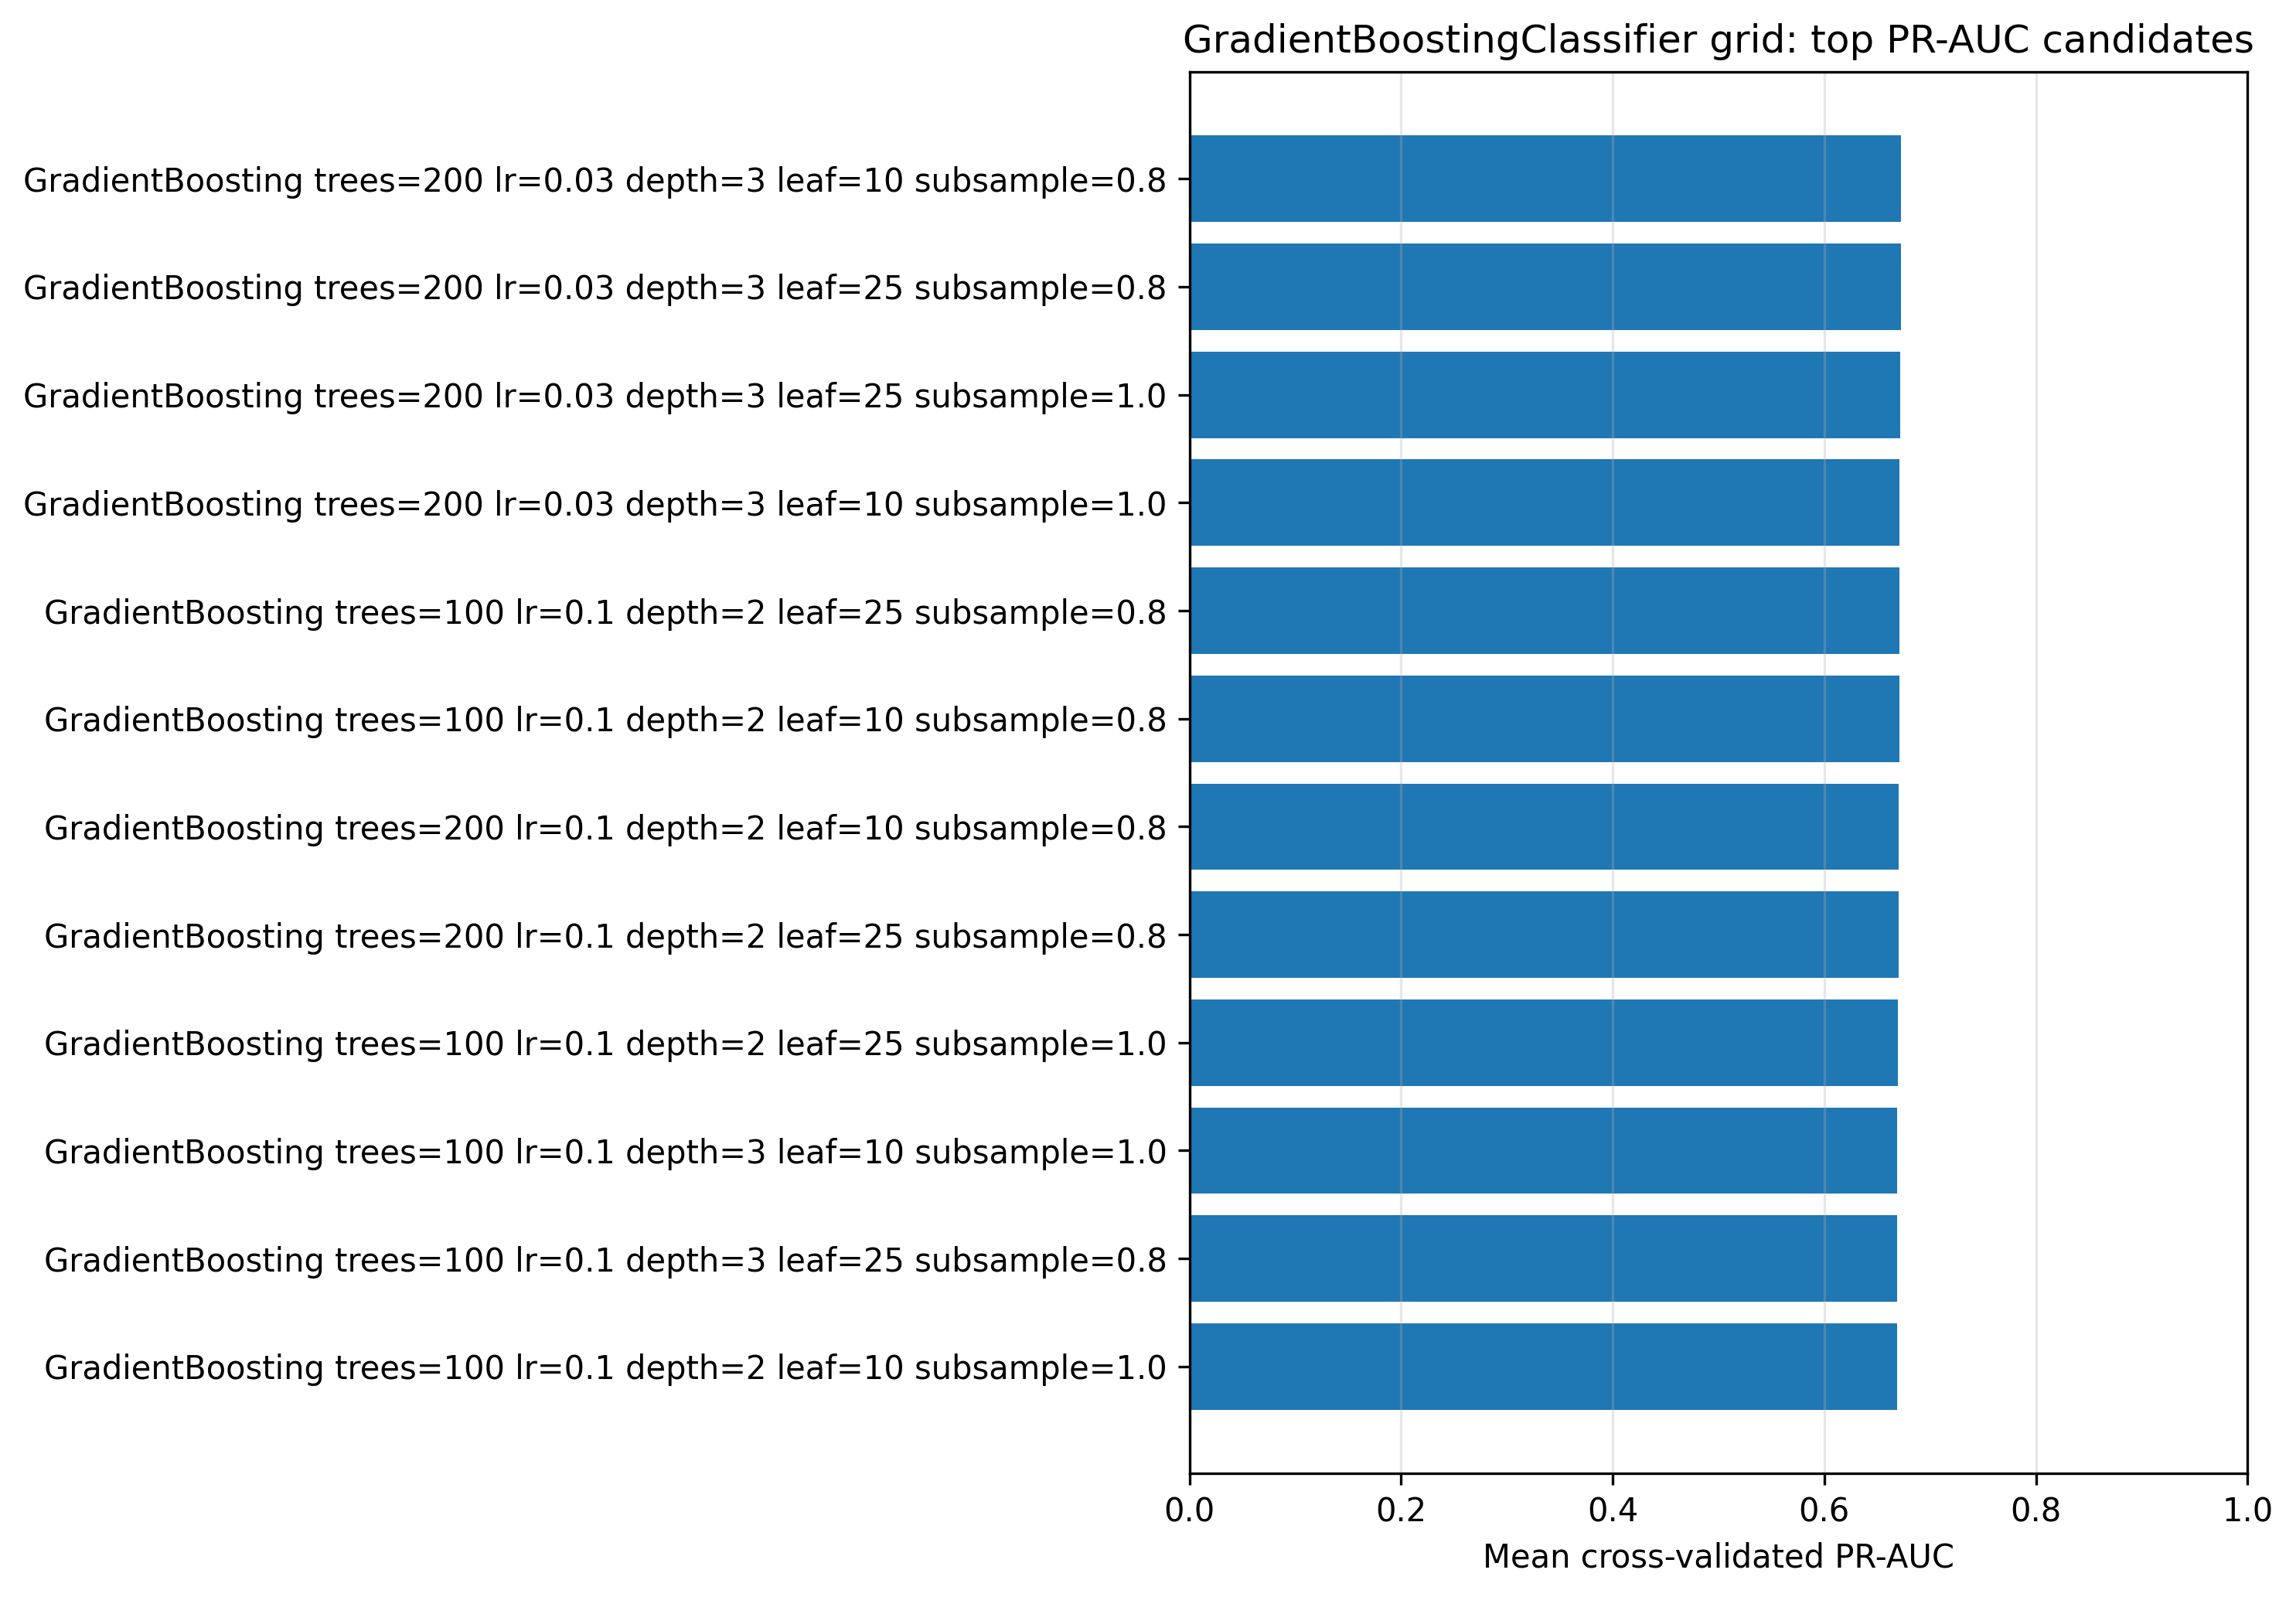
\includegraphics[width=0.88\textwidth]{../figures/gradient_boosting_pr_auc_grid.png}
\caption{GradientBoostingClassifier grid: top cross-validated PR-AUC candidates}
\label{fig:gradient-boosting-pr-auc-grid}
\end{figure}

\begin{figure}[H]
\centering
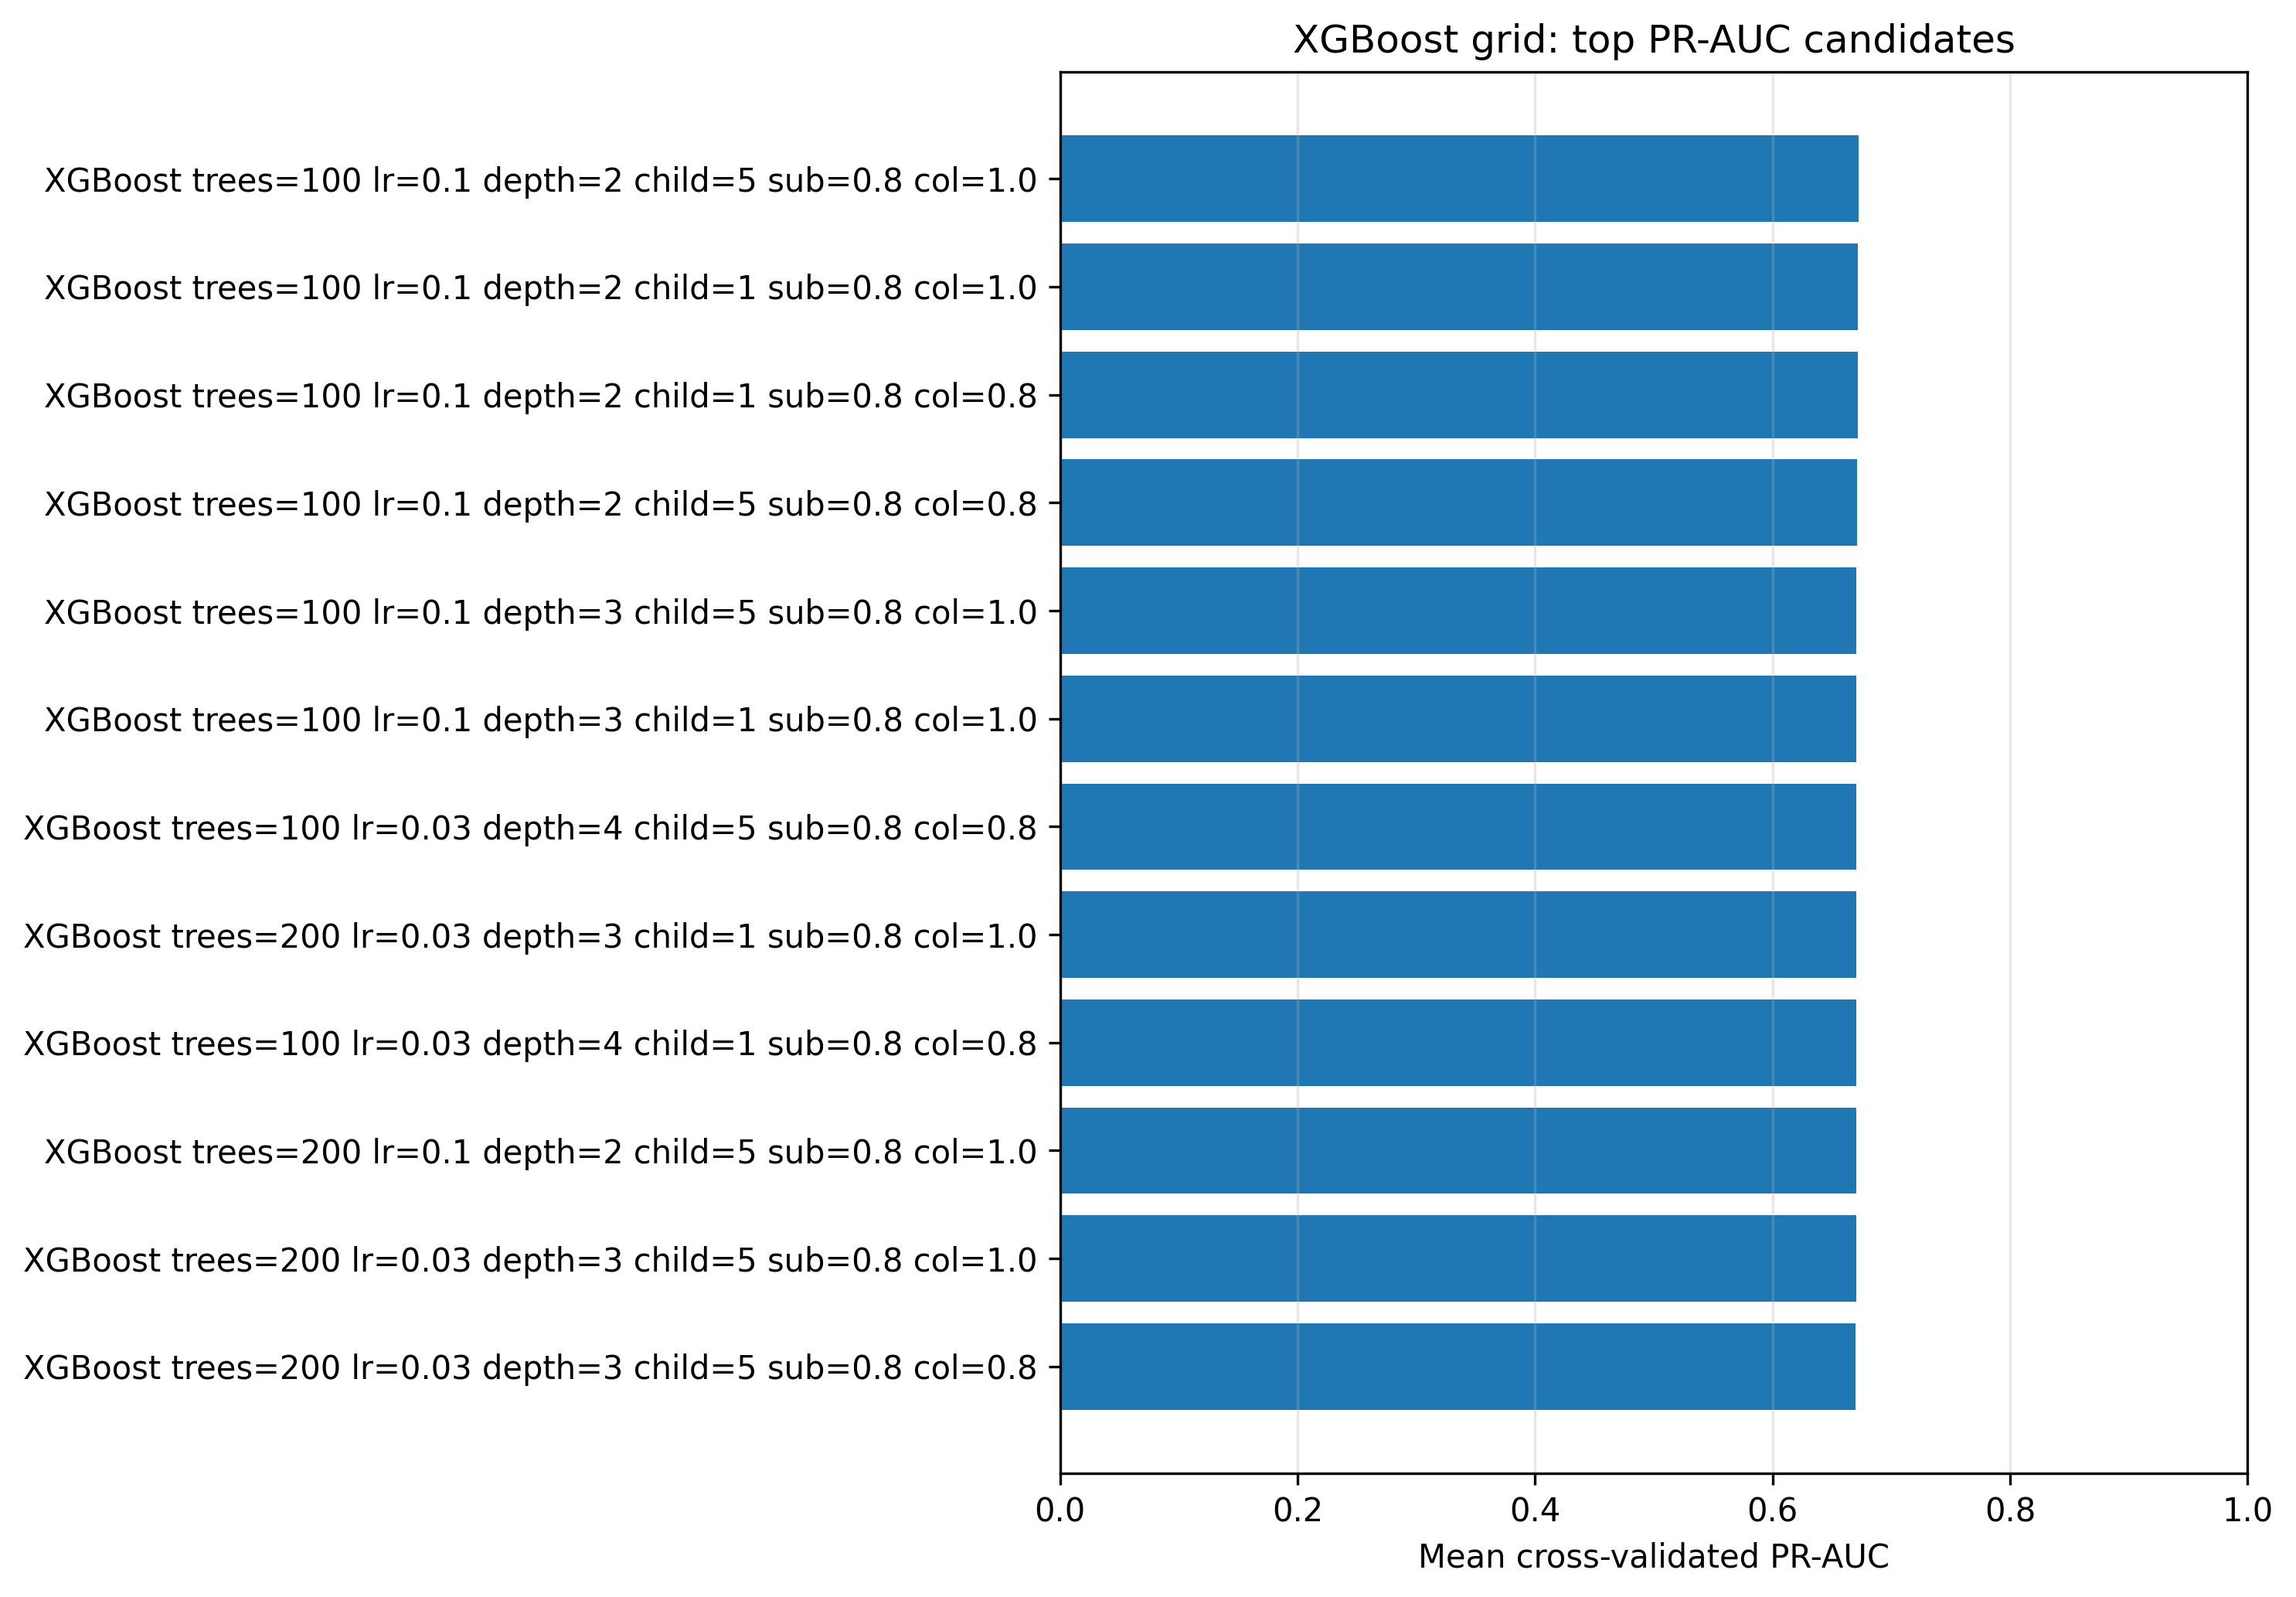
\includegraphics[width=0.88\textwidth]{../figures/xgboost_pr_auc_grid.png}
\caption{XGBoost grid: top cross-validated PR-AUC candidates}
\label{fig:xgboost-pr-auc-grid}
\end{figure}

\begin{figure}[H]
\centering
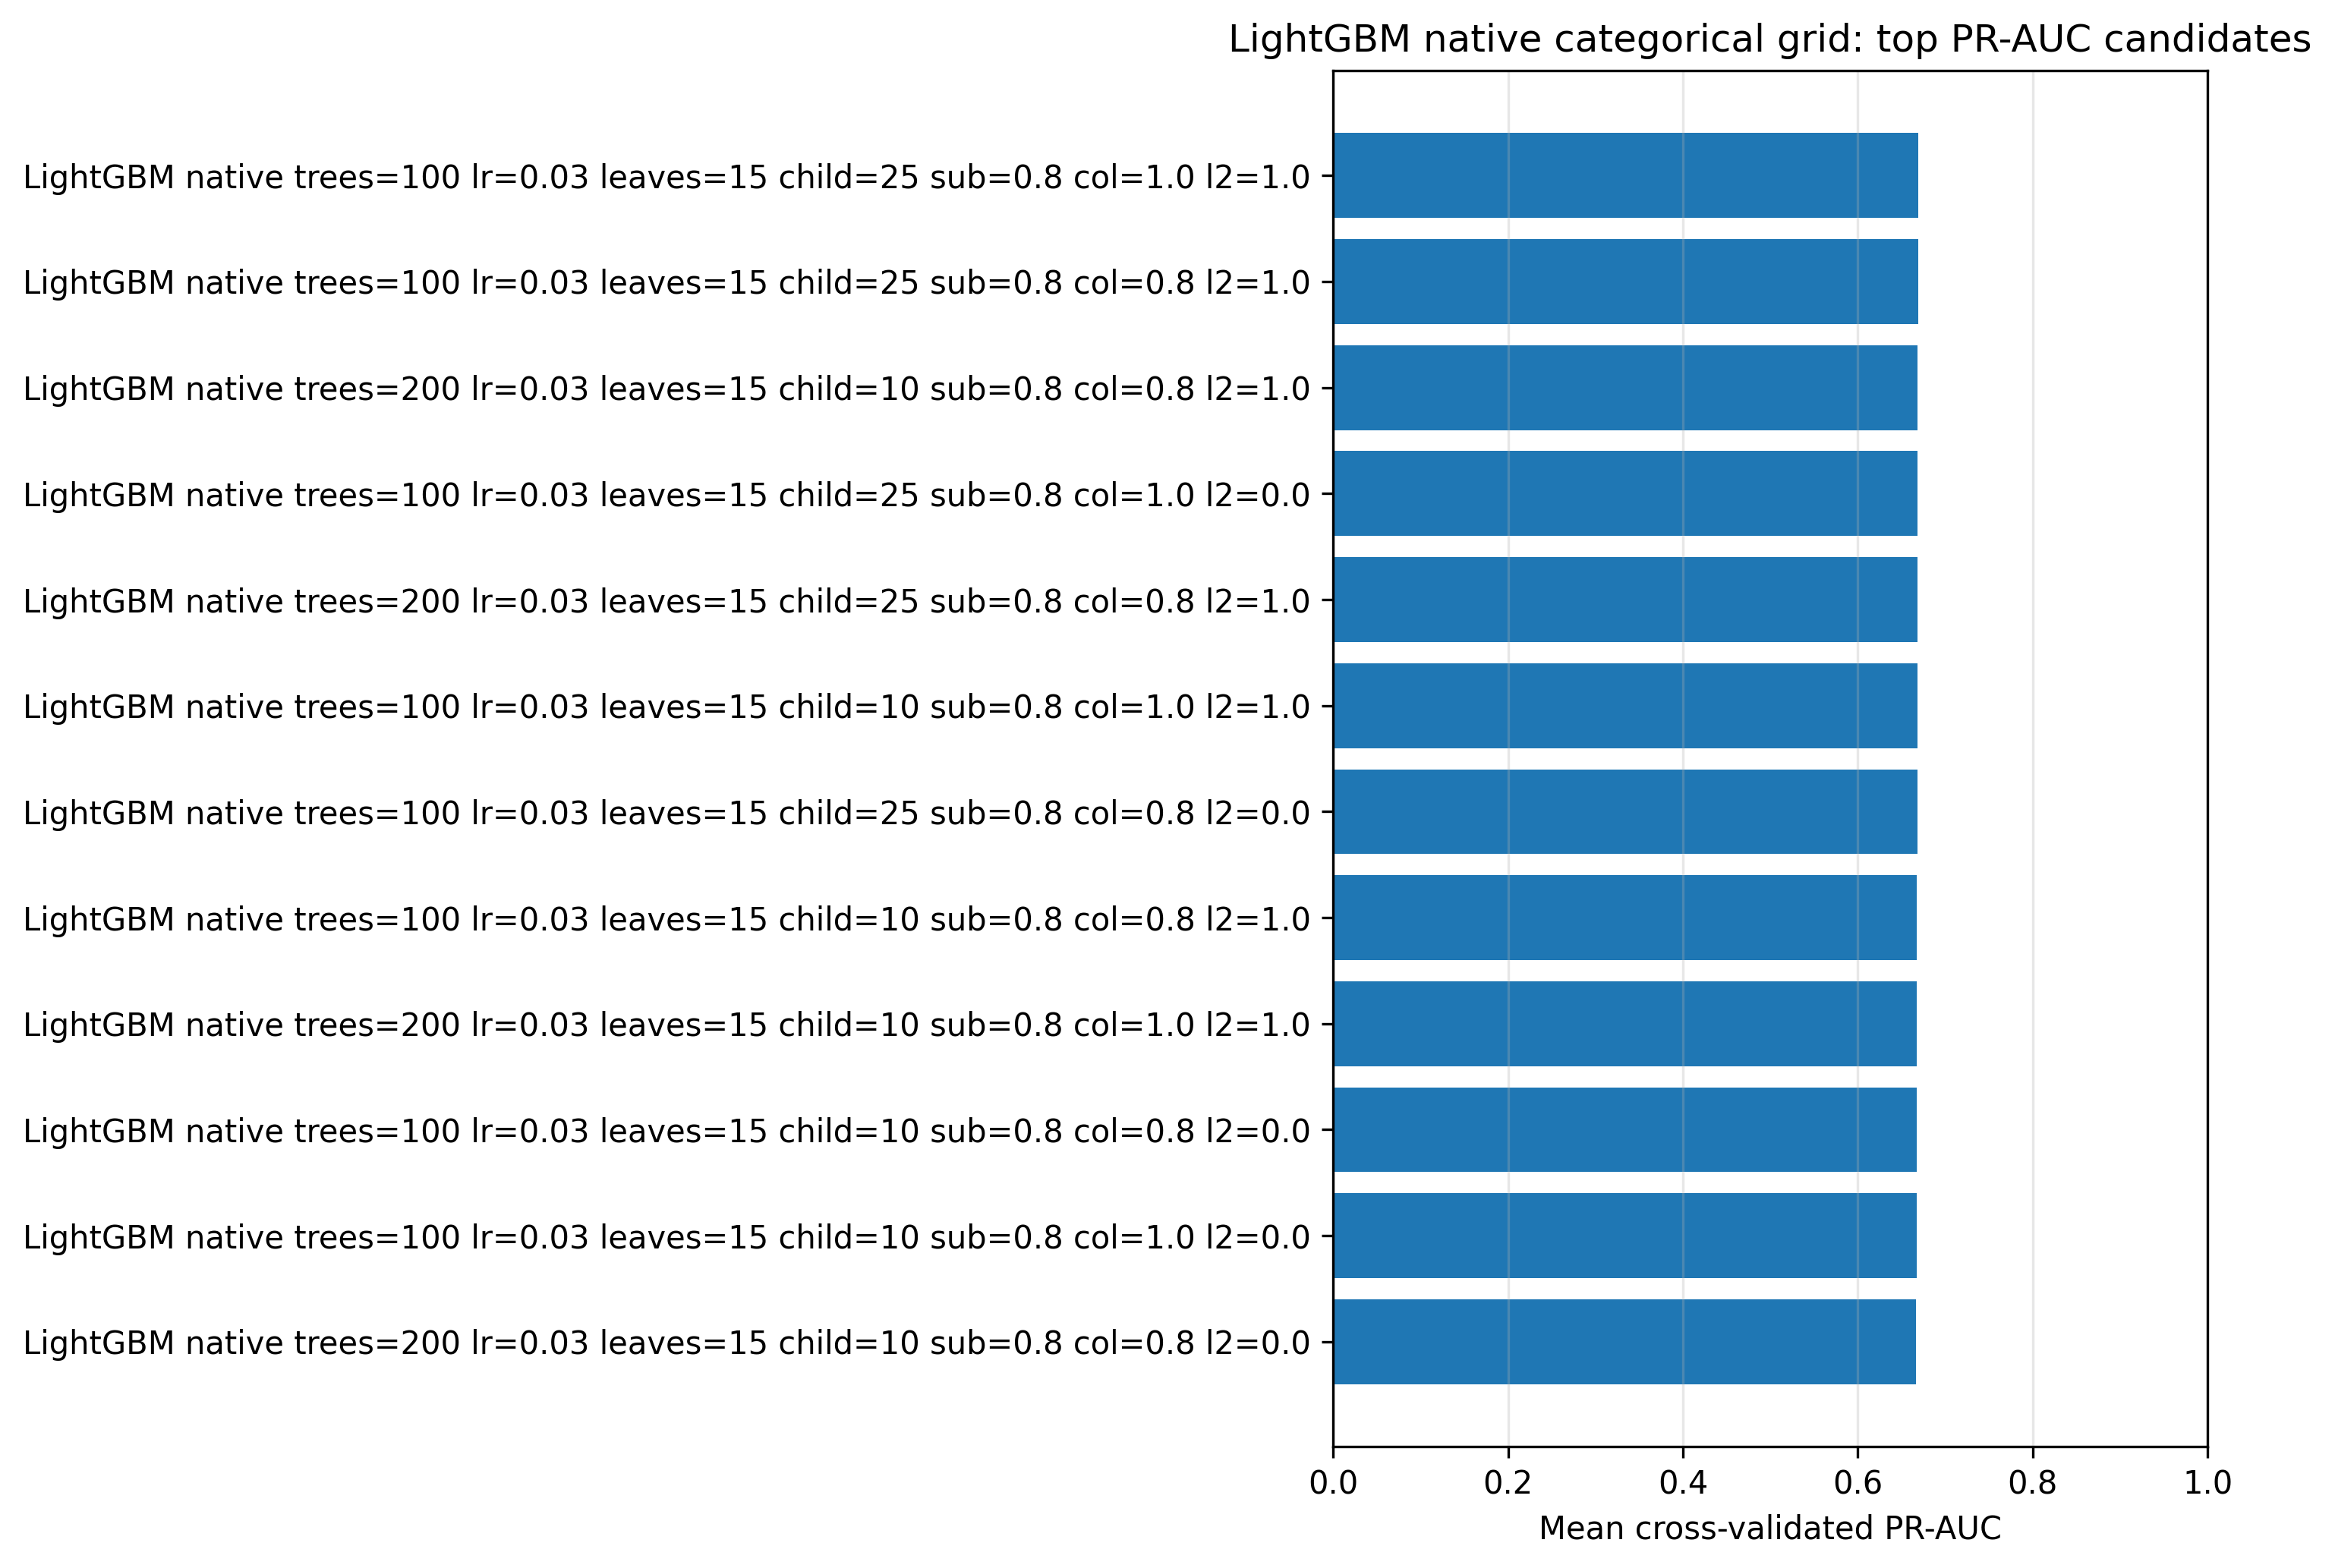
\includegraphics[width=0.88\textwidth]{../figures/lightgbm_pr_auc_grid.png}
\caption{LightGBM native categorical grid: top cross-validated PR-AUC candidates}
\label{fig:lightgbm-pr-auc-grid}
\end{figure}

\begin{figure}[H]
\centering
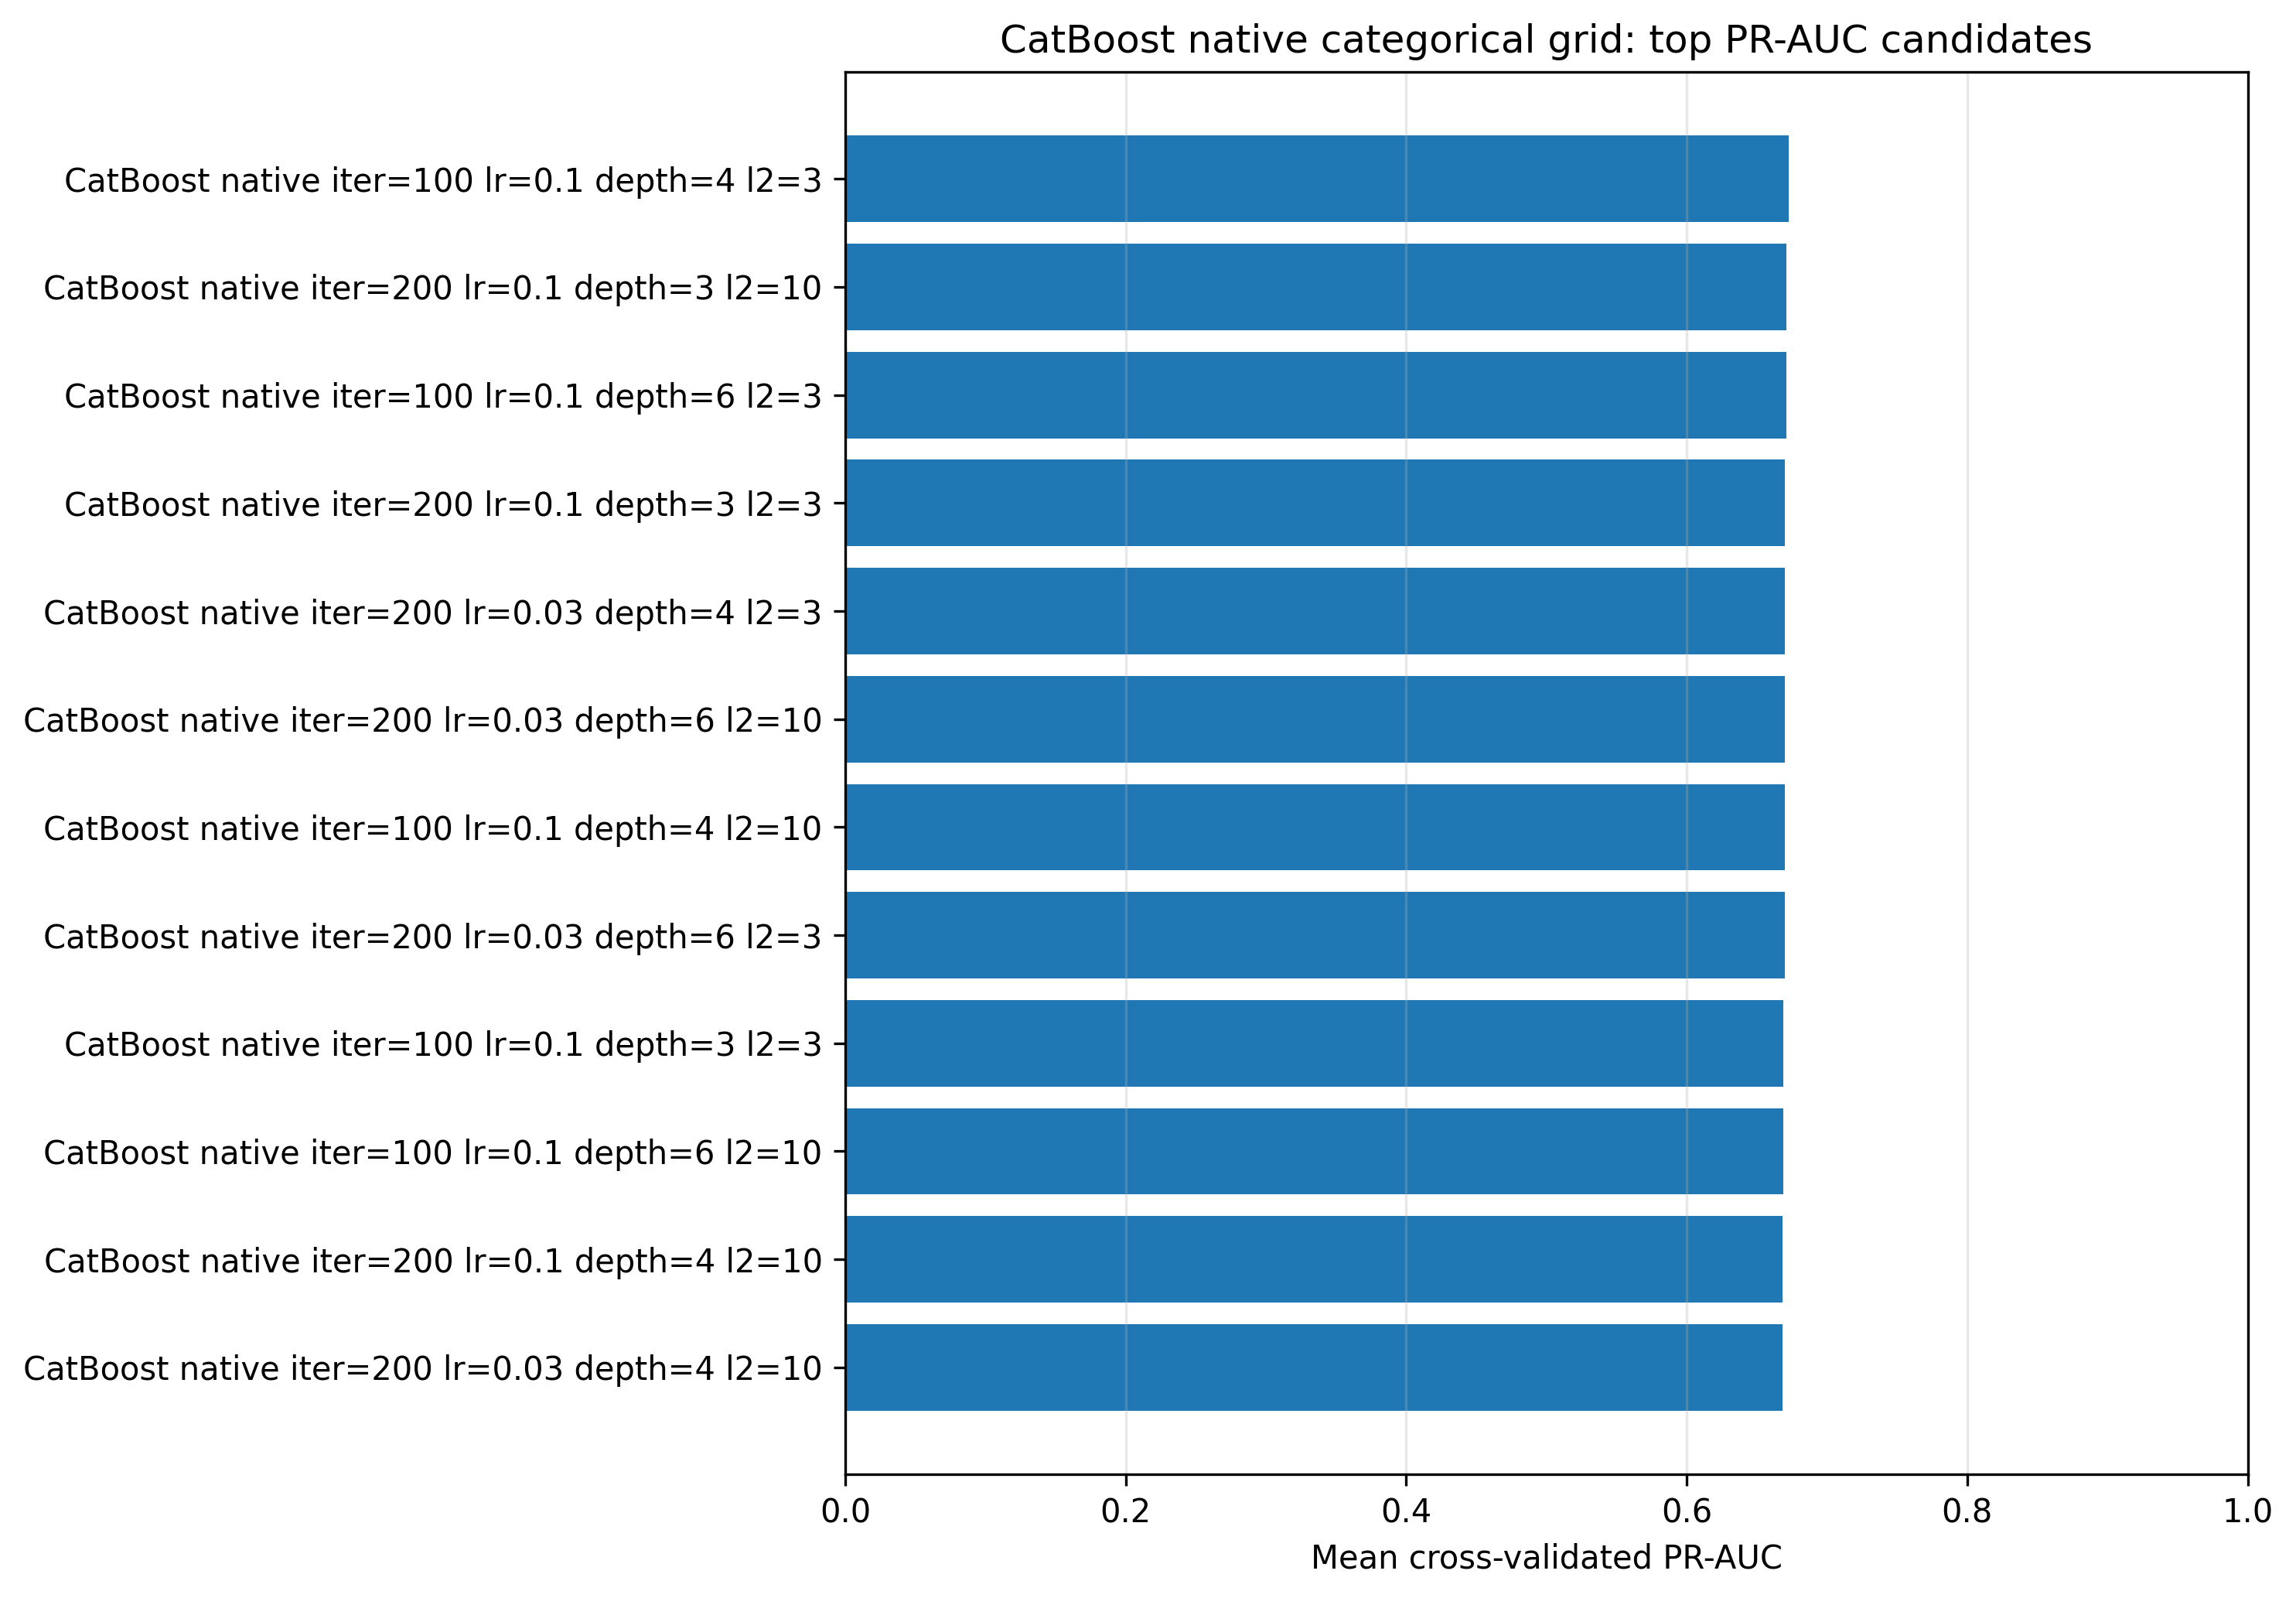
\includegraphics[width=0.88\textwidth]{../figures/catboost_pr_auc_grid.png}
\caption{CatBoost native categorical grid: top cross-validated PR-AUC candidates}
\label{fig:catboost-pr-auc-grid}
\end{figure}

\subsection{Selected candidate comparison}

After selecting one representative candidate from each boosting family, the notebook computes pooled out-of-fold predictions for each candidate and for the previous reference models. Table~\ref{tab:boosting-model-comparison} reports these pooled out-of-fold metrics.

\begin{table}[H]
\centering
\small
\resizebox{\textwidth}{!}{
\begin{tabular}{lrrrrrrrr}
\toprule
Model & Accuracy & Bal. Acc. & Precision & Recall & Specificity & \(F_1\) & ROC-AUC & PR-AUC \\
\midrule
Best XGBoost & 0.808 & 0.722 & 0.671 & 0.539 & 0.905 & 0.598 & 0.850 & 0.670 \\
Best GradientBoostingClassifier & 0.808 & 0.719 & 0.677 & 0.530 & 0.908 & 0.595 & 0.850 & 0.669 \\
Best CatBoost native categorical & 0.807 & 0.717 & 0.676 & 0.525 & 0.909 & 0.591 & 0.850 & 0.669 \\
Best LightGBM native categorical & 0.804 & 0.711 & 0.672 & 0.512 & 0.910 & 0.581 & 0.849 & 0.666 \\
Best AdaBoost & 0.805 & 0.718 & 0.666 & 0.533 & 0.903 & 0.592 & 0.848 & 0.664 \\
Selected bagged trees & 0.800 & 0.705 & 0.662 & 0.504 & 0.907 & 0.572 & 0.846 & 0.662 \\
Selected random forest & 0.804 & 0.706 & 0.678 & 0.498 & 0.914 & 0.574 & 0.847 & 0.660 \\
Best HistGradientBoostingClassifier & 0.807 & 0.719 & 0.671 & 0.532 & 0.906 & 0.594 & 0.848 & 0.660 \\
Selected L2 logistic regression & 0.802 & 0.719 & 0.652 & 0.544 & 0.895 & 0.593 & 0.846 & 0.658 \\
Selected single decision tree & 0.789 & 0.701 & 0.624 & 0.514 & 0.888 & 0.564 & 0.824 & 0.628 \\
\bottomrule
\end{tabular}
}
\caption{Pooled out-of-fold comparison of selected boosting candidates and reference models}
\label{tab:boosting-model-comparison}
\end{table}

Figure~\ref{fig:boosting-model-comparison-pr-auc} shows the same comparison by PR-AUC. XGBoost ranks first in this pooled out-of-fold comparison, with PR-AUC approximately \(0.670\). \texttt{GradientBoostingClassifier} and CatBoost follow extremely closely, both at approximately \(0.669\). LightGBM and AdaBoost are slightly lower, while the selected bagged trees, selected random forest, and selected L2 logistic regression are close to one another around \(0.658\) to \(0.662\). The single decision tree remains clearly weaker by PR-AUC.

\begin{figure}[H]
\centering
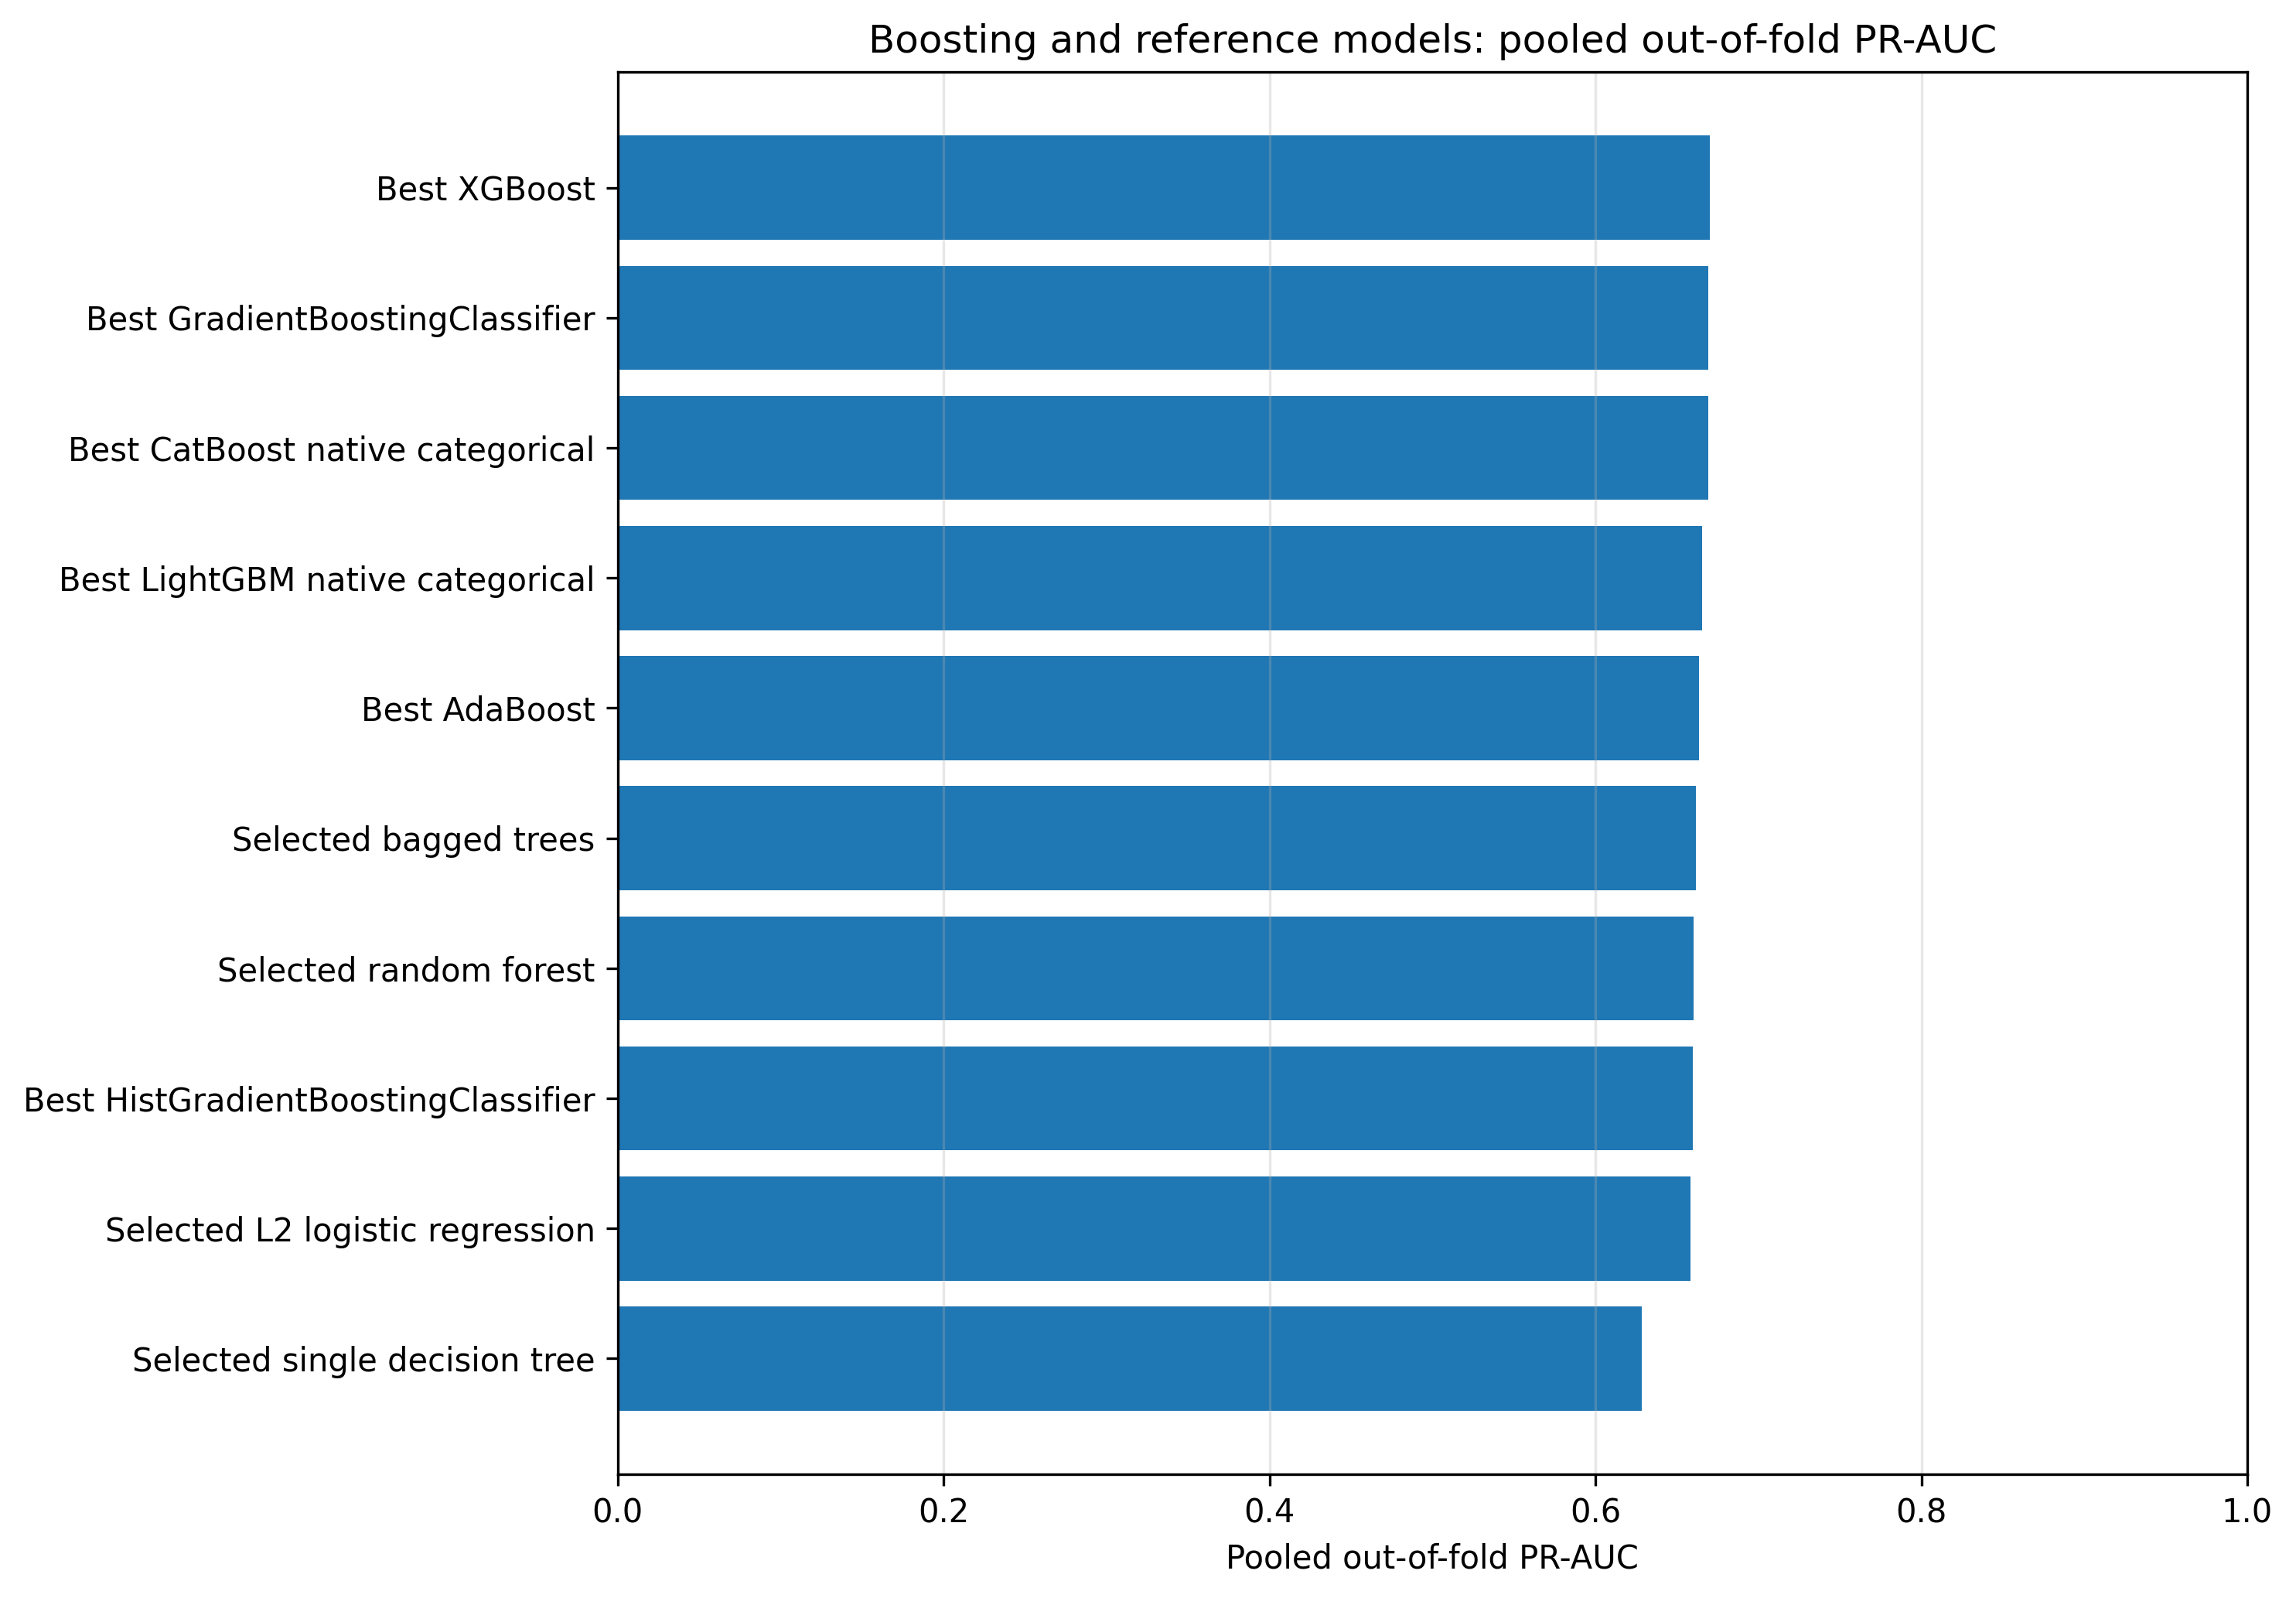
\includegraphics[width=0.88\textwidth]{../figures/boosting_model_comparison_pr_auc.png}
\caption{Boosting and reference models: pooled out-of-fold PR-AUC}
\label{fig:boosting-model-comparison-pr-auc}
\end{figure}

The main conclusion is that boosting forms the strongest development-stage group in this section. The improvement over the single tree is clear. The improvement over bagging, random forests, and logistic regression is more modest. The difference between XGBoost and the next two boosting candidates is too small to claim a meaningful ordering. This section therefore identifies XGBoost as the representative boosting diagnostic model by the chosen pooled out-of-fold PR-AUC rule, but it does not claim that XGBoost has been proven superior to the other leading boosted tree implementations.

\subsection{Confusion-matrix behaviour}

Table~\ref{tab:boosting-confusion-matrices} reports positive-first confusion-matrix counts at the default threshold. The selected XGBoost model detects \(806\) of the \(1495\) churners and produces \(395\) false positives. This corresponds to recall approximately \(0.539\), precision approximately \(0.671\), and a predicted positive rate of approximately \(0.213\), below the observed churn rate of approximately \(0.265\).

\begin{table}[H]
\centering
\small
\resizebox{\textwidth}{!}{
\begin{tabular}{lrrrrr}
\toprule
Model & TP & FN & FP & TN & Pred. positive rate \\
\midrule
Best XGBoost & 806 & 689 & 395 & 3744 & 0.213 \\
Best GradientBoostingClassifier & 793 & 702 & 379 & 3760 & 0.208 \\
Best CatBoost native categorical & 785 & 710 & 377 & 3762 & 0.206 \\
Best LightGBM native categorical & 765 & 730 & 373 & 3766 & 0.202 \\
Best AdaBoost & 797 & 698 & 400 & 3739 & 0.212 \\
Selected bagged trees & 753 & 742 & 385 & 3754 & 0.202 \\
Selected random forest & 744 & 751 & 354 & 3785 & 0.195 \\
Best HistGradientBoostingClassifier & 796 & 699 & 391 & 3748 & 0.211 \\
Selected L2 logistic regression & 813 & 682 & 434 & 3705 & 0.221 \\
Selected single decision tree & 769 & 726 & 463 & 3676 & 0.219 \\
\bottomrule
\end{tabular}
}
\caption{Positive-first pooled out-of-fold confusion-matrix counts for selected boosting candidates and reference models}
\label{tab:boosting-confusion-matrices}
\end{table}

The default-threshold behaviour shows that many of the strongest candidates are relatively conservative. They flag fewer customers than the observed churn proportion. Logistic regression detects slightly more churners at the default threshold, but it also produces more false positives and has lower PR-AUC than the top boosting models. This reinforces the distinction between ranking performance and operating-threshold performance. A model can rank customers well while still requiring a threshold adjustment if the business objective prioritizes recall.

\subsection{Threshold behaviour for the selected XGBoost model}

The selected XGBoost model is used for threshold diagnostics because it has the highest pooled out-of-fold PR-AUC in Table~\ref{tab:boosting-model-comparison}. Table~\ref{tab:boosting-threshold-results} reports selected thresholds. Lower thresholds recover more churners but also flag many more non-churners. Higher thresholds increase precision and specificity but miss more churners.

\begin{table}[H]
\centering
\small
\begin{tabular}{rrrrrr}
\toprule
Threshold & Precision & Recall & Specificity & \(F_1\) & Pred. positive rate \\
\midrule
0.100 & 0.406 & 0.940 & 0.504 & 0.567 & 0.614 \\
0.200 & 0.485 & 0.865 & 0.669 & 0.622 & 0.473 \\
0.250 & 0.512 & 0.824 & 0.716 & 0.631 & 0.427 \\
0.300 & 0.541 & 0.771 & 0.763 & 0.636 & 0.378 \\
0.350 & 0.572 & 0.716 & 0.806 & 0.636 & 0.332 \\
0.400 & 0.611 & 0.655 & 0.849 & 0.632 & 0.285 \\
0.500 & 0.671 & 0.539 & 0.905 & 0.598 & 0.213 \\
0.600 & 0.718 & 0.379 & 0.946 & 0.496 & 0.140 \\
\bottomrule
\end{tabular}
\caption{Threshold behaviour for the selected XGBoost model using pooled out-of-fold scores}
\label{tab:boosting-threshold-results}
\end{table}

At the default threshold \(0.50\), precision is about \(0.671\), recall is about \(0.539\), and \(F_1\) is about \(0.598\). Lowering the threshold to \(0.30\) increases recall to about \(0.771\) and gives \(F_1\) about \(0.636\), but precision falls to about \(0.541\). A threshold near \(0.25\) gives even higher recall, about \(0.824\), but flags approximately \(42.7\%\) of customers. These patterns are expected for an imbalanced churn problem. A lower threshold can be reasonable if missed churners are expensive, but the final threshold should not be chosen in this section. It depends on intervention costs, retention value, capacity constraints, calibration, and final model comparison.

Figure~\ref{fig:boosting-threshold-tradeoff} visualizes the same tradeoff.

\begin{figure}[H]
\centering
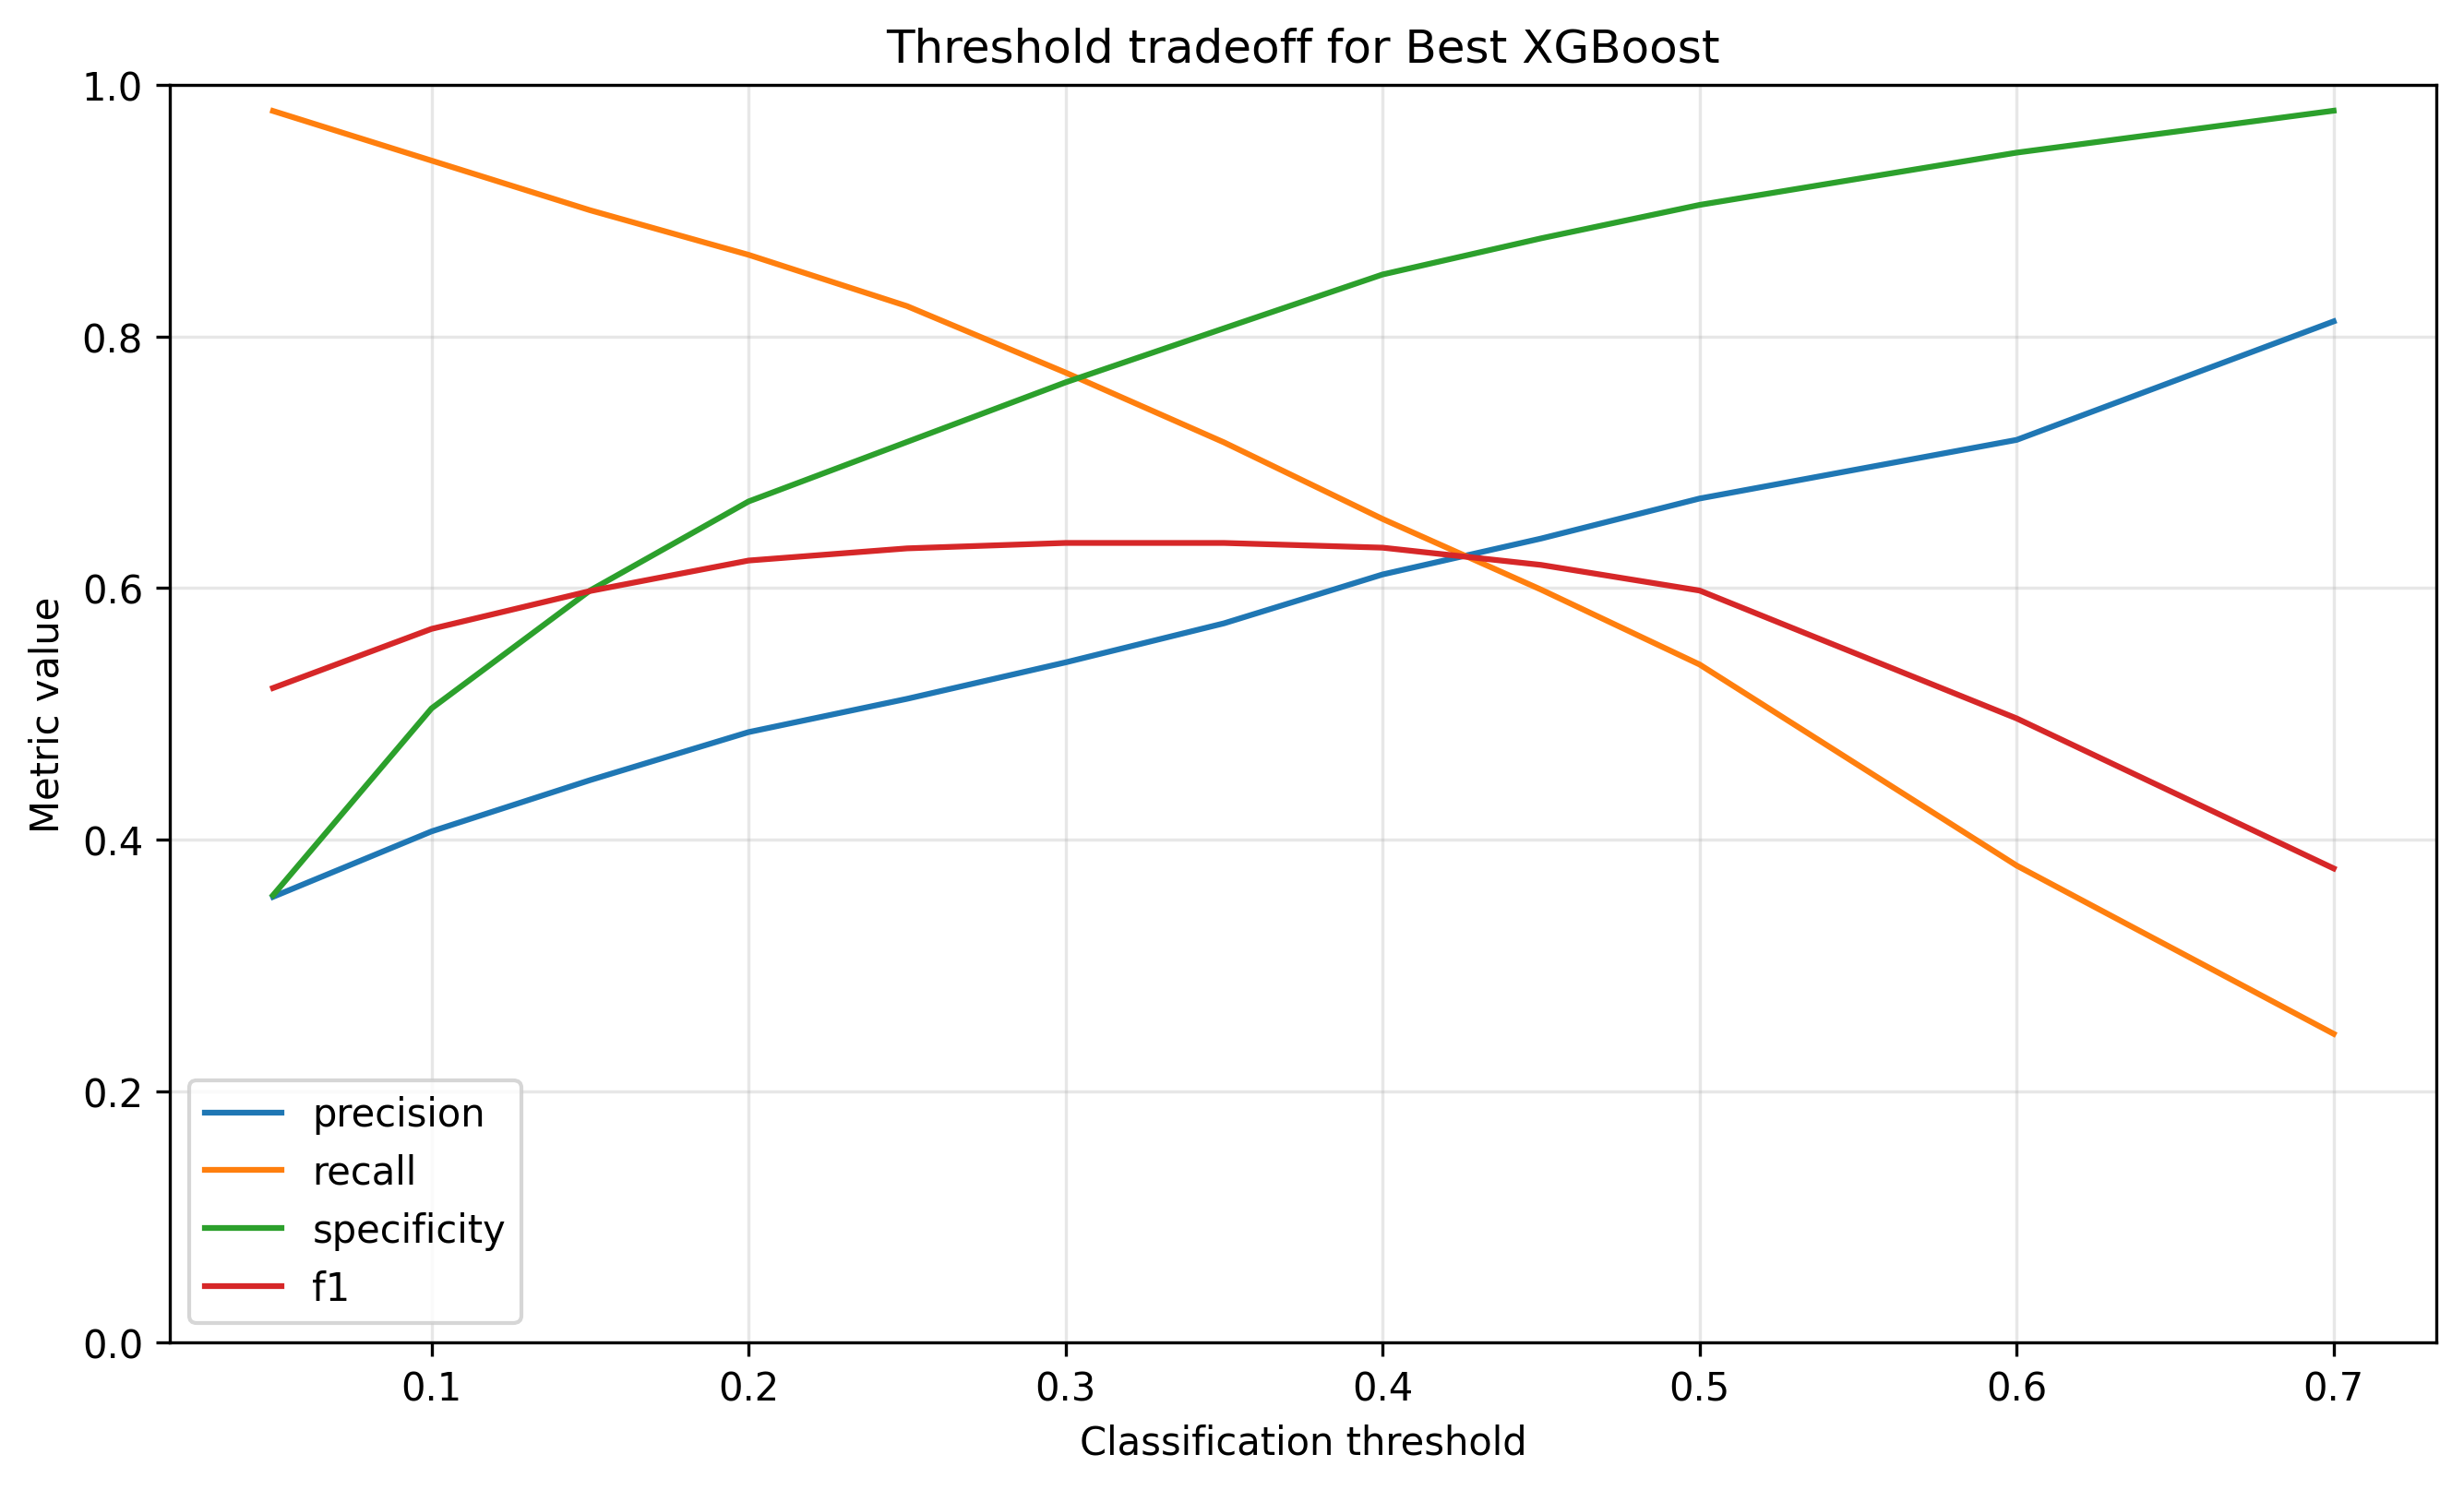
\includegraphics[width=0.88\textwidth]{../figures/boosting_threshold_tradeoff.png}
\caption{Threshold tradeoff for the selected XGBoost model}
\label{fig:boosting-threshold-tradeoff}
\end{figure}

\subsection{Ranking curves}

Figures~\ref{fig:boosting-roc-curve} and~\ref{fig:boosting-pr-curve} show the ROC and precision-recall curves for the selected XGBoost model. The ROC-AUC is approximately \(0.850\), while the PR-AUC is approximately \(0.670\). The precision-recall curve remains well above the positive-rate baseline of approximately \(0.265\) over much of the recall range, indicating that the model produces useful churn-risk rankings.

\begin{figure}[H]
\centering
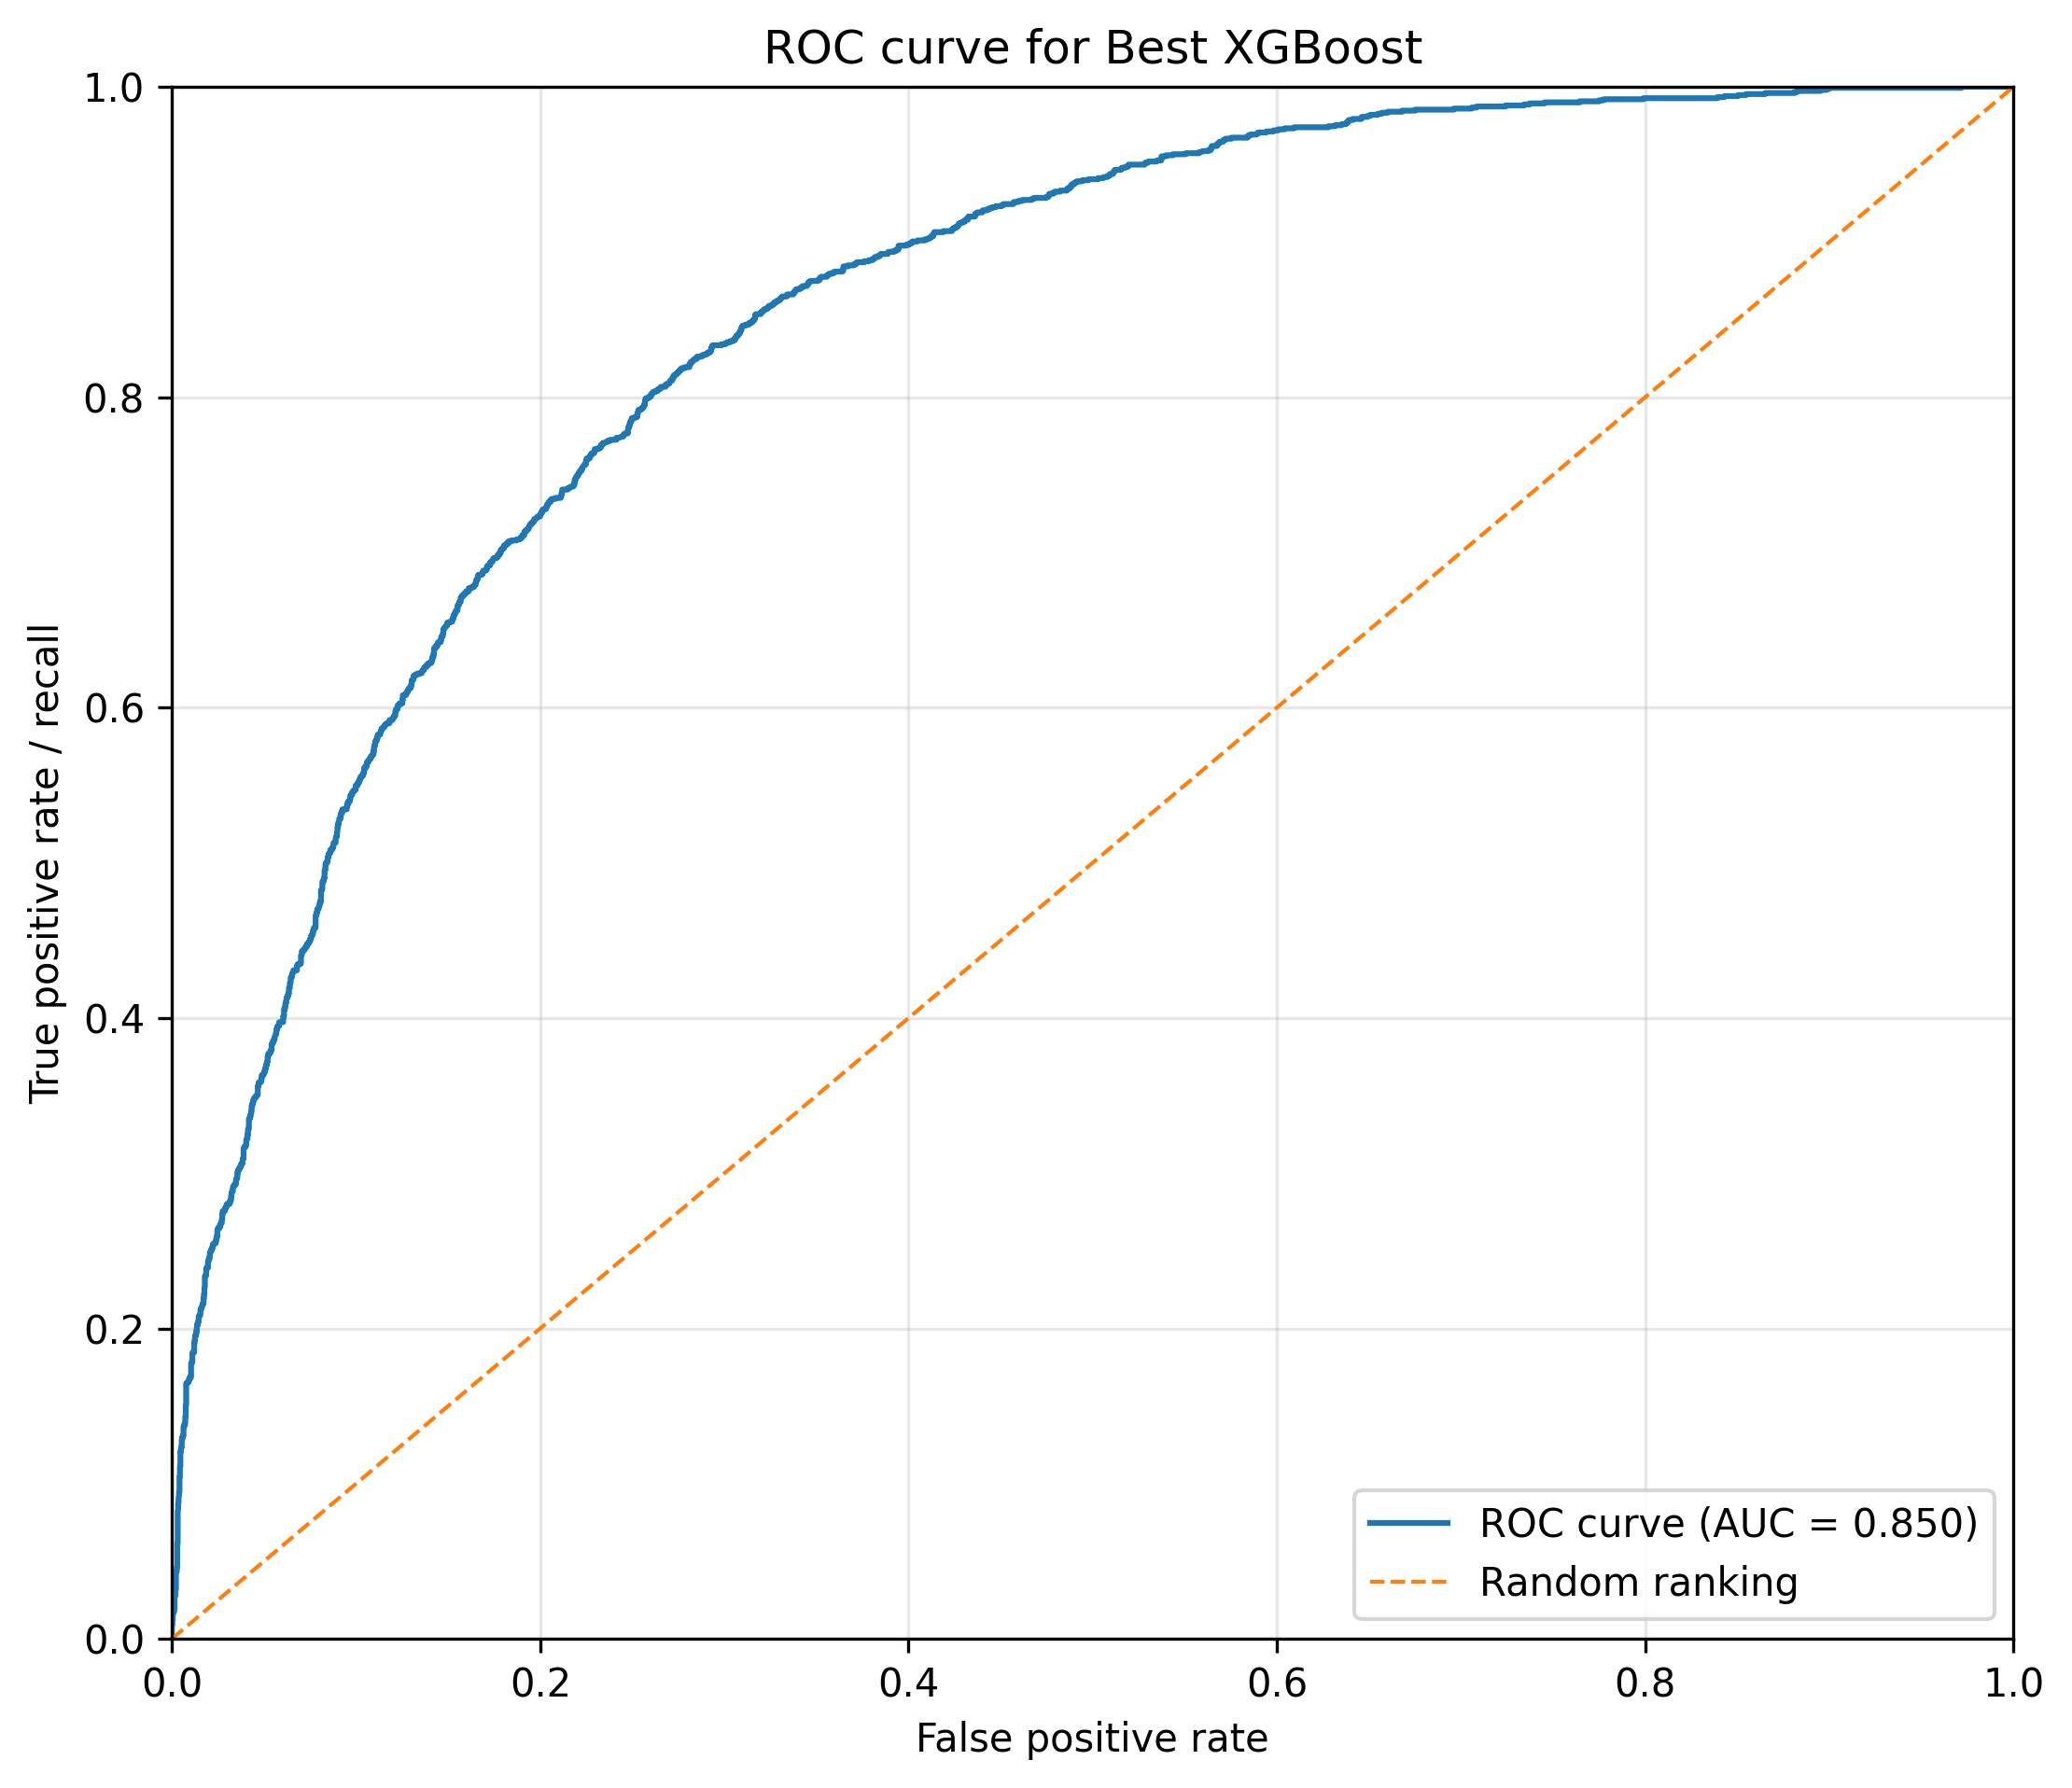
\includegraphics[width=0.82\textwidth]{../figures/boosting_roc_curve.png}
\caption{ROC curve for the selected XGBoost model}
\label{fig:boosting-roc-curve}
\end{figure}

\begin{figure}[H]
\centering
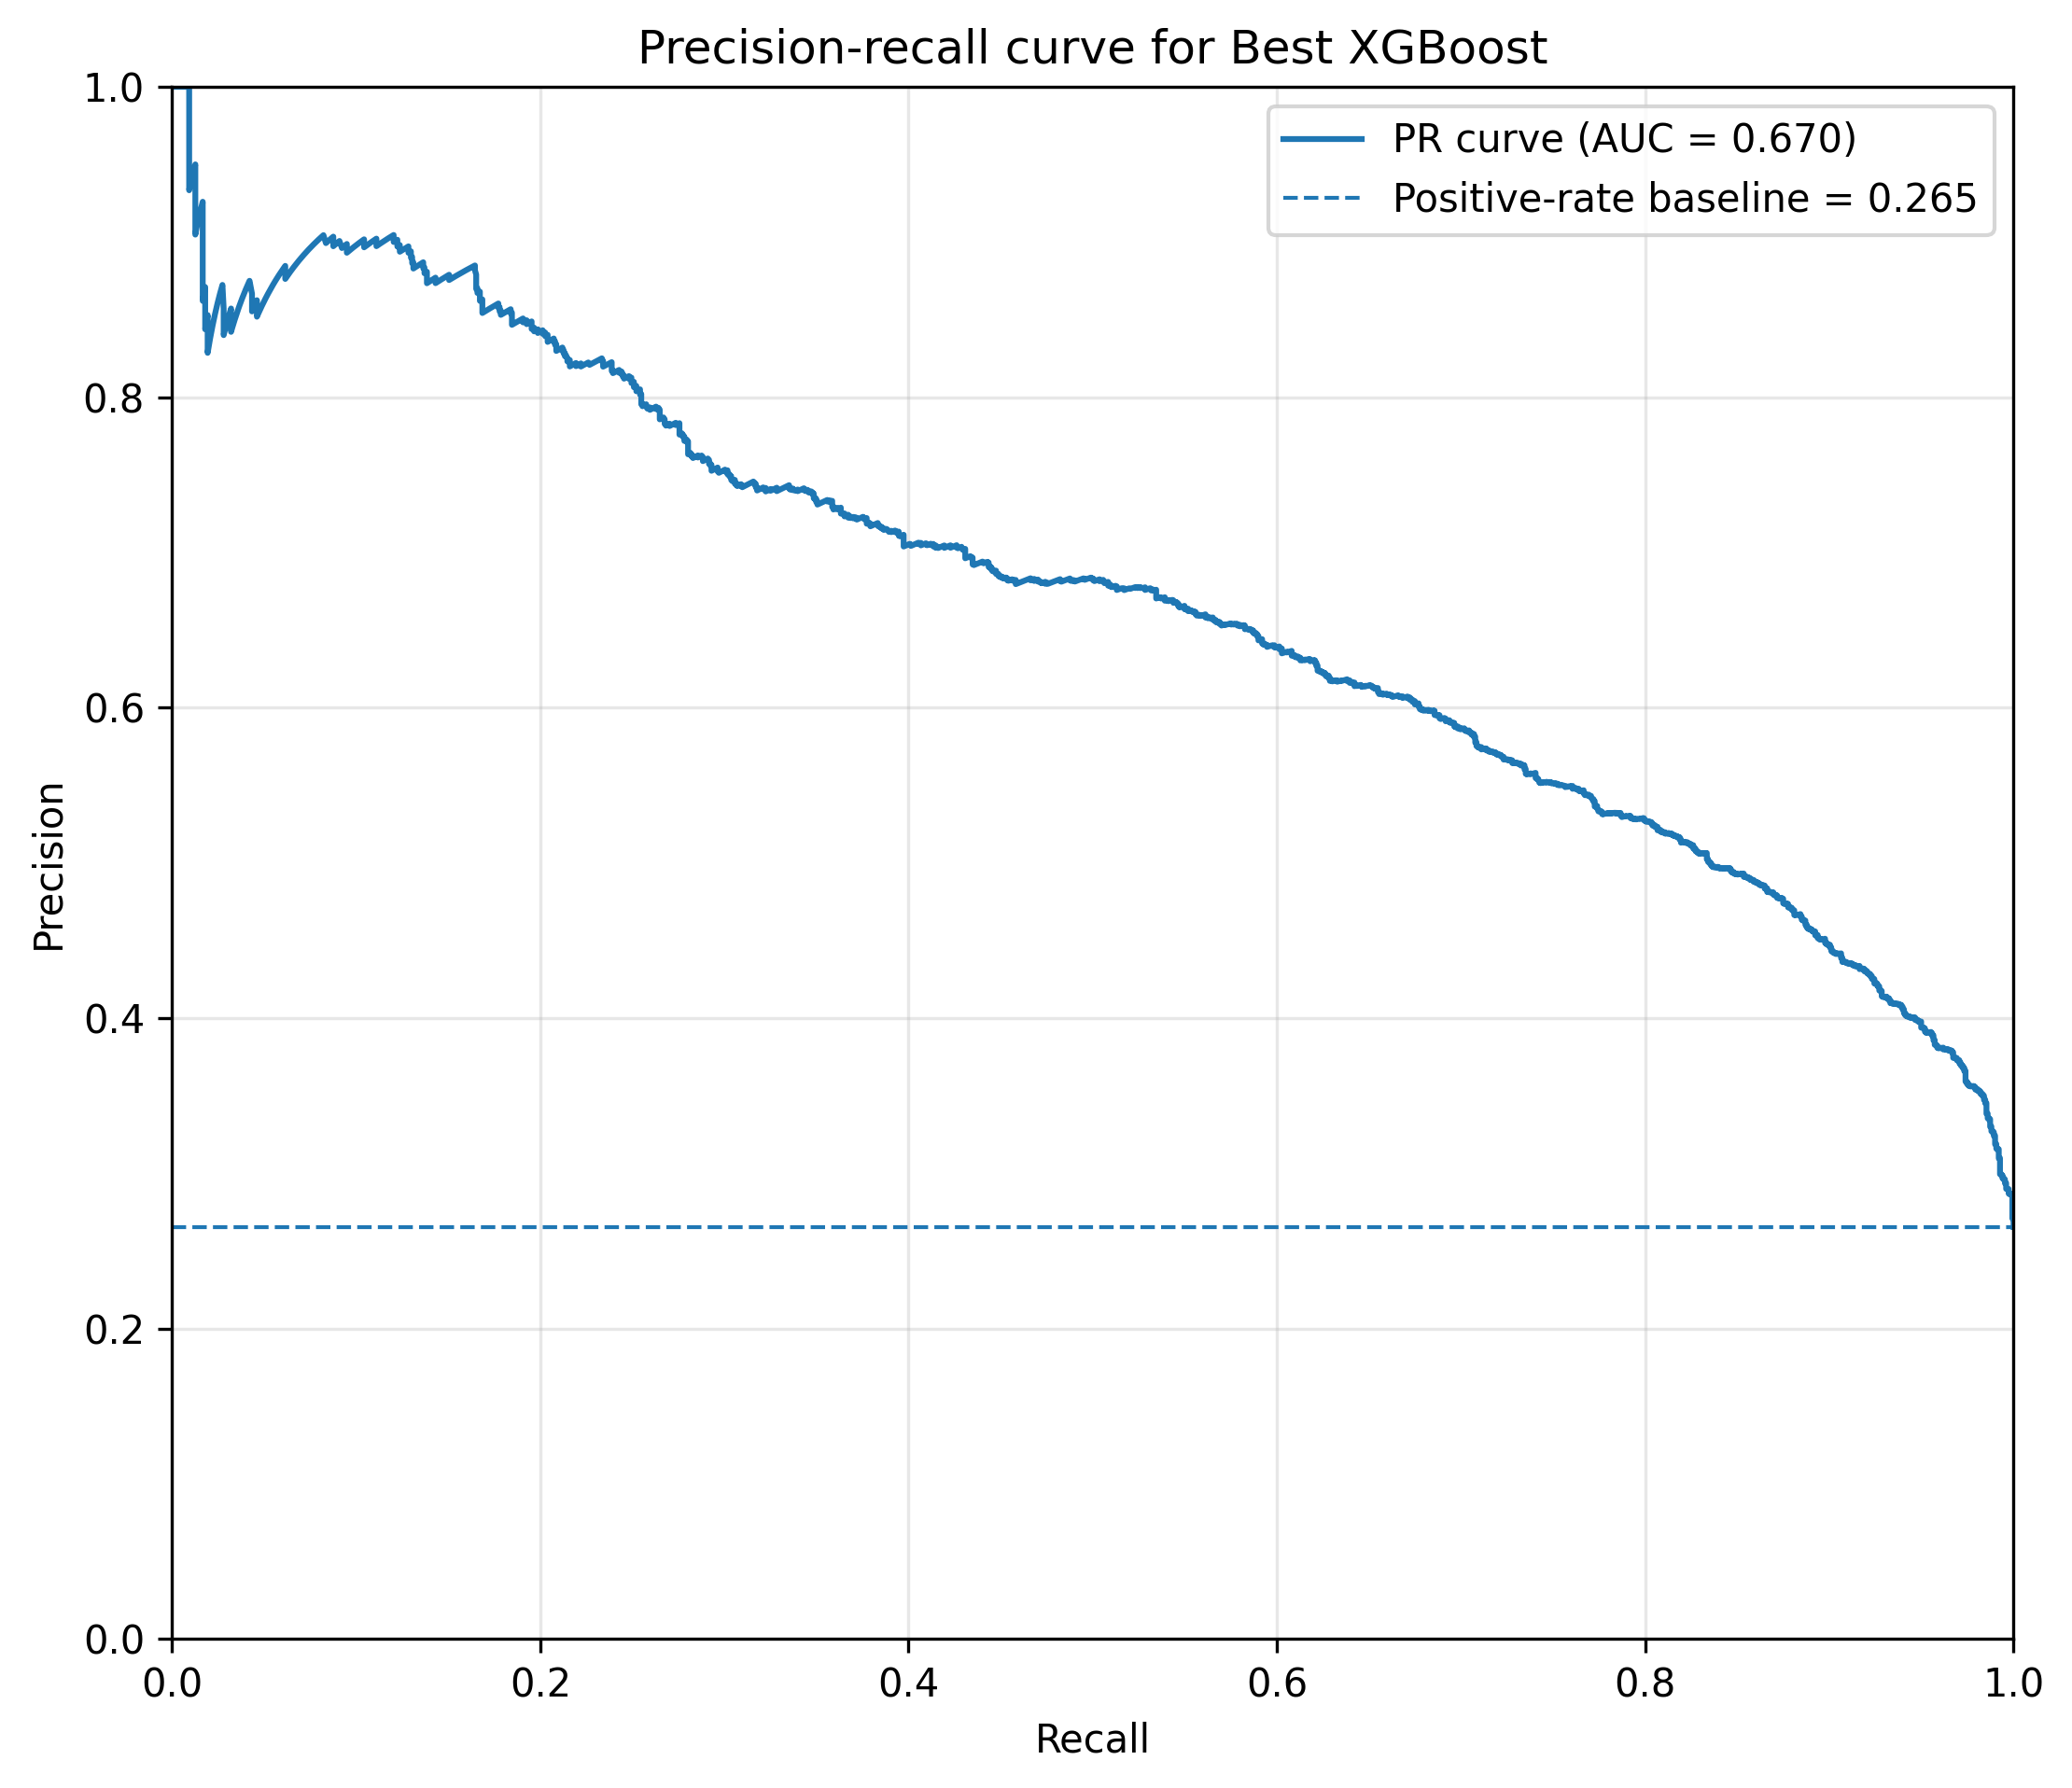
\includegraphics[width=0.82\textwidth]{../figures/boosting_precision_recall_curve.png}
\caption{Precision-recall curve for the selected XGBoost model}
\label{fig:boosting-pr-curve}
\end{figure}

The PR curve is especially relevant because churn is the positive minority class. The curve shows that precision is high for the top-ranked customers, then declines as recall approaches one. This is the normal shape of a useful risk-ranking model: the highest-score customers are enriched for churn, while extending intervention to lower-score customers gradually approaches the base churn rate.

\subsection{Feature importance}

Feature importance is computed by refitting selected boosting candidates on the full training set. This refit is used only for interpretation and does not enter the performance estimates. For the selected XGBoost model, the largest importance is assigned to the month-to-month contract indicator. Other important predictors include online security absence, fiber optic internet service, electronic-check payment, tech-support absence, long-term contract indicators, and tenure.

\begin{table}[H]
\centering
\small
\begin{tabular}{lr}
\toprule
Feature & Importance \\
\midrule
Contract\_Month-to-month & 0.418 \\
OnlineSecurity\_No & 0.104 \\
InternetService\_Fiber optic & 0.100 \\
PaymentMethod\_Electronic check & 0.071 \\
TechSupport\_No & 0.060 \\
Contract\_Two year & 0.036 \\
tenure & 0.028 \\
StreamingTV\_Yes & 0.021 \\
PaperlessBilling\_No & 0.019 \\
Contract\_One year & 0.016 \\
\bottomrule
\end{tabular}
\caption{Top feature importances for the selected XGBoost model}
\label{tab:boosting-feature-importance}
\end{table}

\begin{figure}[H]
\centering
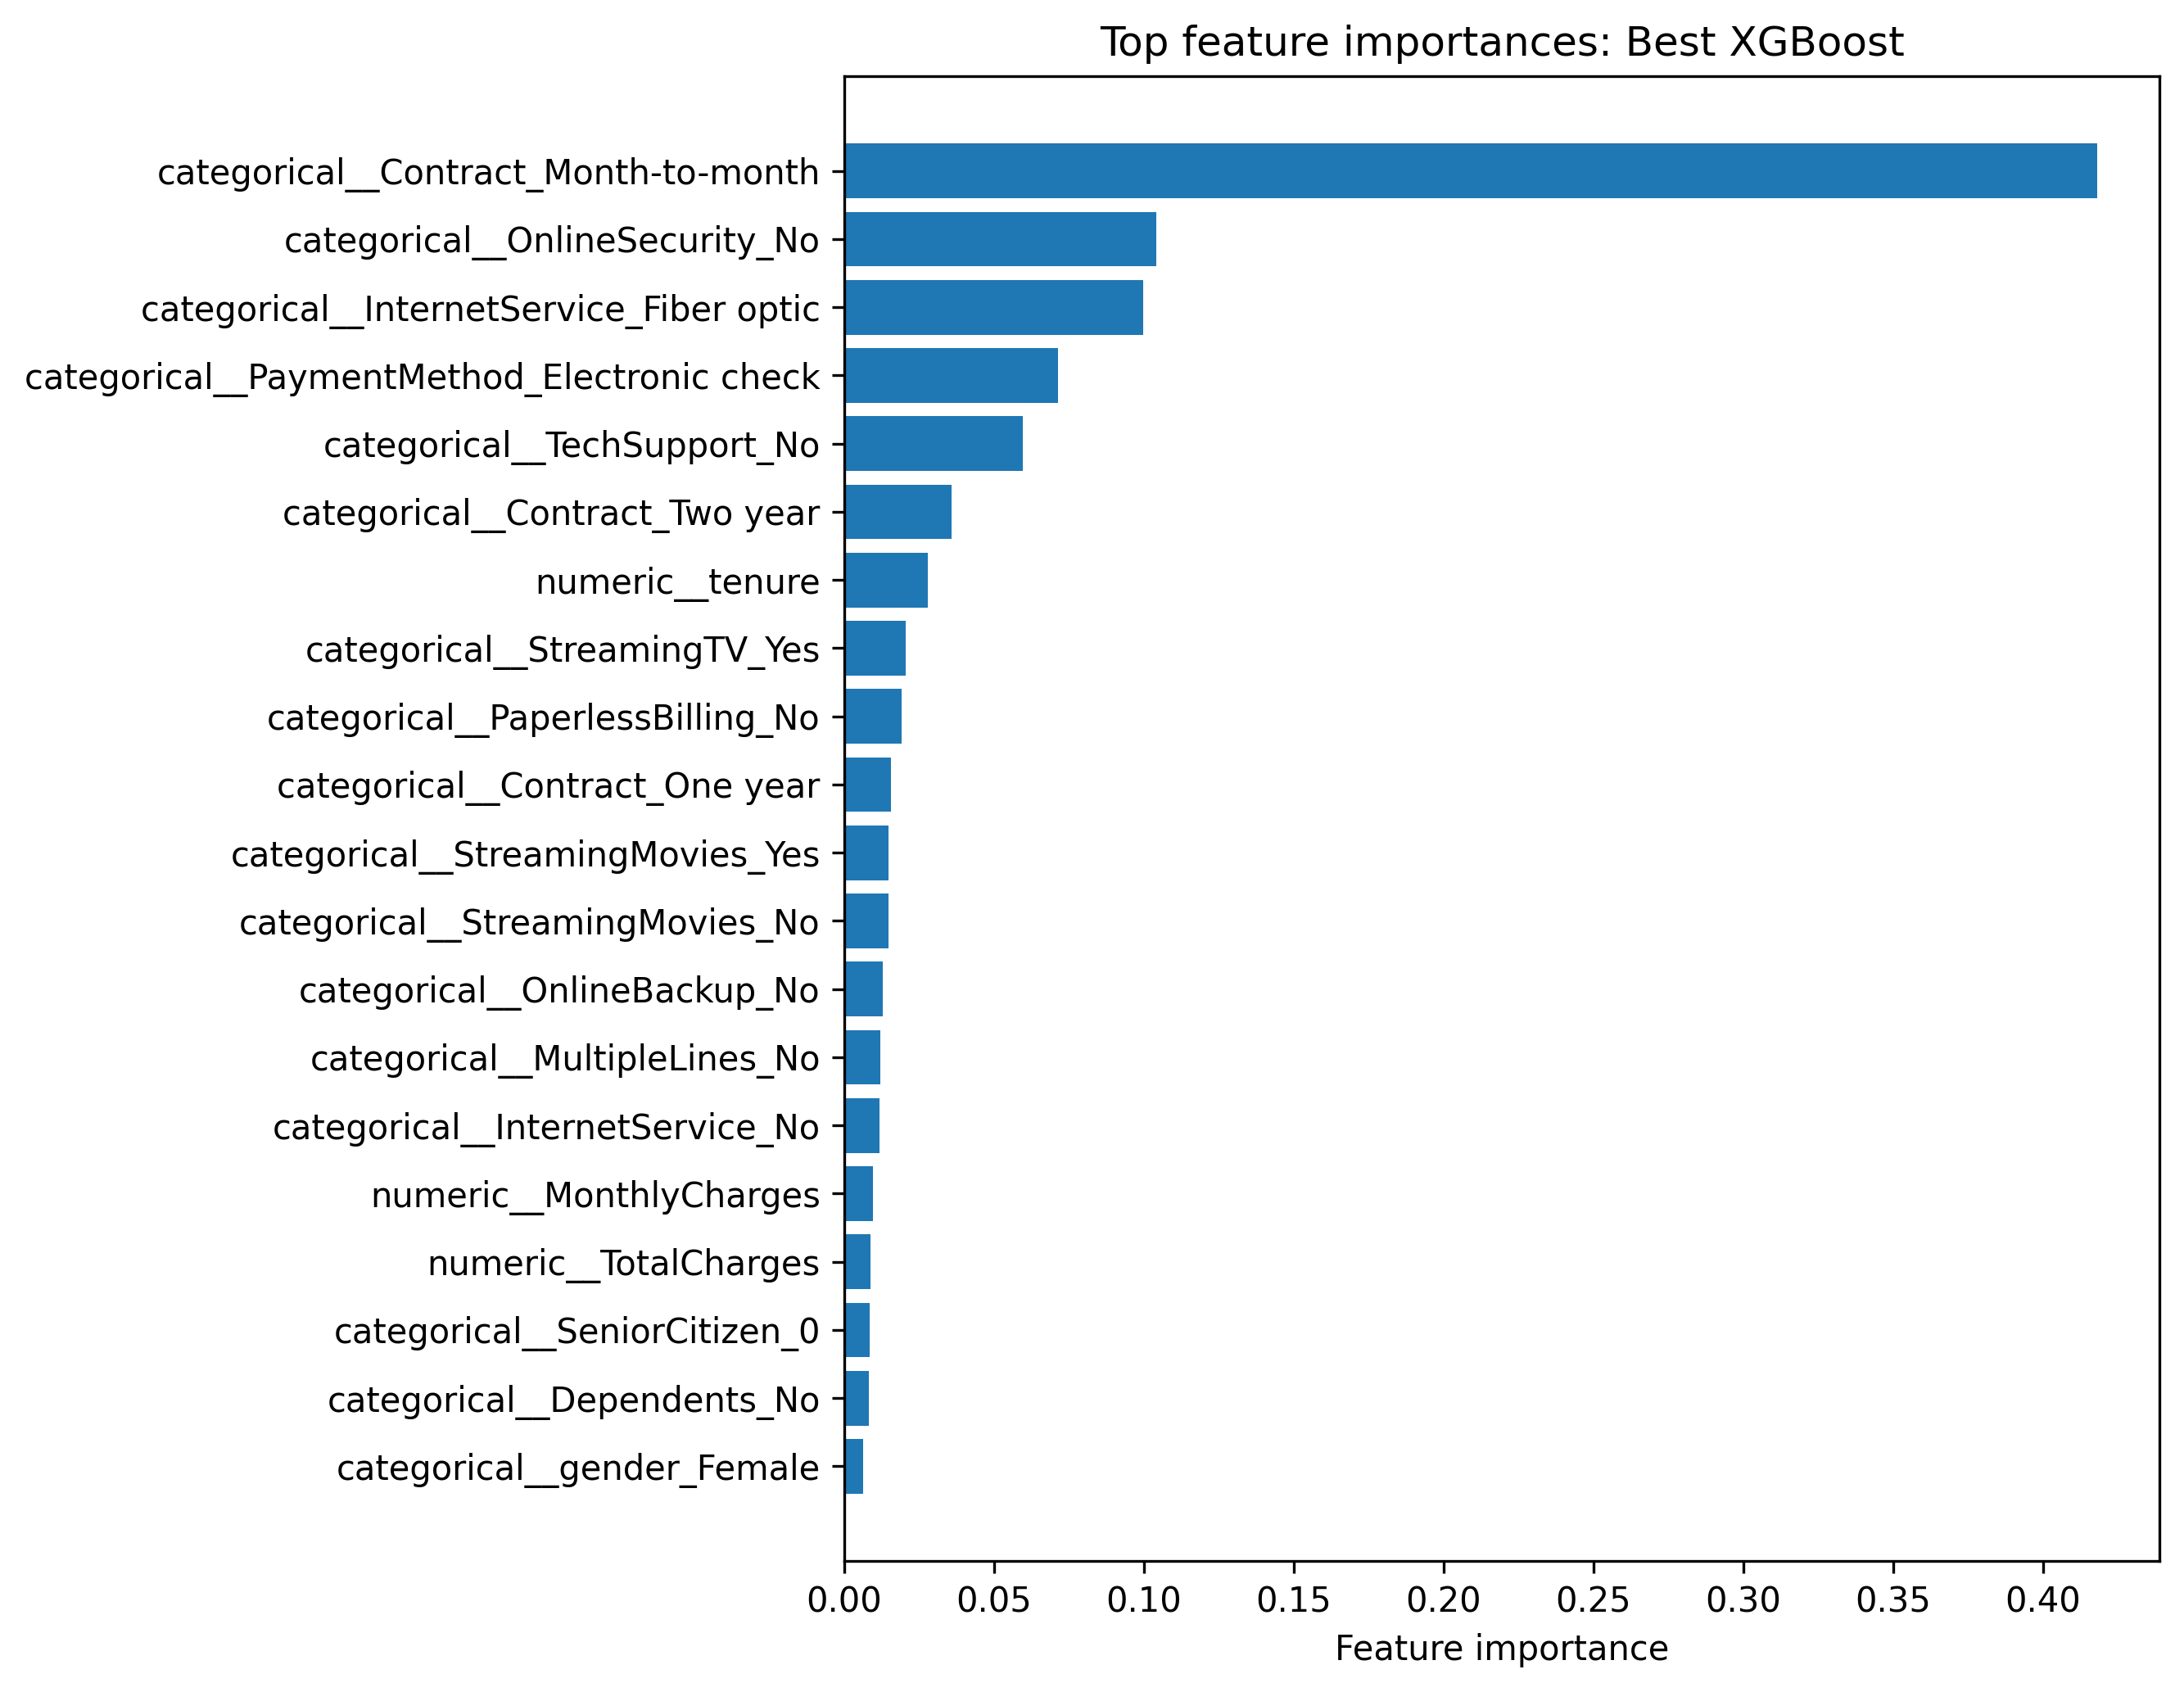
\includegraphics[width=0.84\textwidth]{../figures/boosting_feature_importance.png}
\caption{Top feature importances for the selected XGBoost model}
\label{fig:boosting-feature-importance}
\end{figure}

These importances are consistent with earlier sections. Contract type, tenure, internet service, online security, tech support, and payment method have repeatedly appeared as strong churn-related predictors. The feature importance values should not be interpreted causally. They describe how this fitted boosted-tree model uses features for prediction, not what would happen if a customer changed contract type or payment method.

\subsection{Section summary}

Boosting extends the tree-based modelling sequence by moving from independent averaging to sequential additive correction. The evaluated models include classical AdaBoost, scikit-learn gradient boosting, histogram gradient boosting, XGBoost, LightGBM, and CatBoost.

The development-stage results show that boosting is a strong model family for this tabular churn problem. The selected XGBoost candidate has the highest pooled out-of-fold PR-AUC, approximately \(0.670\), followed very closely by \texttt{GradientBoostingClassifier} and CatBoost. The fixed-grid selection table gives CatBoost the highest mean CV PR-AUC, but the difference relative to XGBoost and GradientBoosting is extremely small. The safe conclusion is therefore that boosted tree methods form a strong group, not that one specific implementation has been proven best.

Compared with earlier references, boosting clearly improves over the single decision tree and modestly improves over the selected bagged trees, selected random forest, and selected L2 logistic regression. The improvement is meaningful enough to keep boosted trees as serious final candidates, but not large enough to ignore uncertainty, tuning fairness, threshold selection, or calibration. Those issues remain part of the later final model-comparison stage, which will compare the strongest model families under a more deliberate training-only selection procedure before the held-out test set is used.


\newpage
\newpage
\section{Support Vector Machines: Maximum-Margin Classification and Kernel Methods}
\label{sec:support-vector-machines}

This section evaluates support vector machines (SVMs) for churn prediction. The previous sections considered probability-based linear classifiers, nearest-neighbour methods, probabilistic models, individual decision trees, bagging, random forests, and boosting. SVMs provide a distinct modelling principle. Rather than estimating a conditional probability directly, an SVM constructs a decision boundary and seeks a boundary with a large separation margin between the two classes.

The held-out test set is not used in this section. All tuning, selection, figures, tables, and comparisons are based on stratified cross-validation within the training set. The reported configurations are therefore development-stage candidates selected within transparent fixed grids. They are not final globally optimized models and they do not provide final held-out test performance.

\subsection{Linear decision scores and separating hyperplanes}

For a binary classification problem, a linear SVM starts with the score
\[
f(x) = w^\top x + b,
\]
where \(x\) is the transformed feature vector, \(w\) is the coefficient vector, and \(b\) is an intercept. The decision boundary is the hyperplane
\[
w^\top x + b = 0.
\]
For labels coded as \(y_i \in \{-1,+1\}\), the sign of the score determines the predicted class:
\[
\widehat{y}_i = \operatorname{sign}(f(x_i)).
\]

The numerical value of \(f(x)\) is a signed decision score. A large positive score places an observation on the positive-class side of the boundary, while a large negative score places it on the negative-class side. Unlike logistic regression, the raw score is not a calibrated probability. This distinction is important later when interpreting score thresholds.

\subsection{Maximum margin and support vectors}

A separating hyperplane is not unique when the classes can be separated. SVMs select a separator by maximizing the margin, namely the distance between the boundary and the closest training observations. Under the conventional scaling of the score, the two margin boundaries are
\[
w^\top x + b = +1
\qquad \text{and} \qquad
w^\top x + b = -1.
\]
Their distance is
\[
\frac{2}{\lVert w \rVert}.
\]

For perfectly separable data, the hard-margin SVM solves
\[
\min_{w,b} \frac{1}{2}\lVert w \rVert^2
\]
subject to
\[
y_i(w^\top x_i+b)\geq 1,
\qquad i=1,\ldots,n.
\]
Minimizing \(\lVert w\rVert^2\) maximizes the margin. The observations that lie on the margin, or violate it in the nonseparable case, are the \emph{support vectors}. They determine the fitted boundary most directly.

Hard-margin separation is usually too restrictive for real churn data. Classes overlap, predictors contain noise, and some customer profiles are difficult to classify. The practical model is therefore the soft-margin SVM.

\subsection{Soft margins, hinge loss, and regularization}

The soft-margin SVM introduces non-negative slack variables \(\xi_i\):
\[
\min_{w,b,\xi}
\frac{1}{2}\lVert w\rVert^2
+
C\sum_{i=1}^{n}\xi_i
\]
subject to
\[
y_i(w^\top x_i+b)\geq 1-\xi_i,
\qquad
\xi_i\geq 0.
\]
The parameter \(C>0\) controls the tradeoff between a wide, regularized margin and penalties for observations that lie inside the margin or on the wrong side of the boundary. Smaller \(C\) values impose stronger regularization and tolerate more margin violations. Larger \(C\) values penalize violations more strongly and can create a more flexible, higher-variance boundary.

The same principle can be written through hinge loss:
\[
\ell_{\mathrm{hinge}}(y_i,f(x_i))
=
\max\{0,1-y_i f(x_i)\}.
\]
The corresponding unconstrained objective is
\[
\min_{w,b}
\frac{1}{2}\lVert w\rVert^2
+
C\sum_{i=1}^{n}
\max\{0,1-y_i f(x_i)\}.
\]

The notebook evaluates both the standard hinge loss and the squared-hinge variant exposed by \texttt{LinearSVC}:
\[
\ell_{\mathrm{squared\ hinge}}(y_i,f(x_i))
=
\left[
\max\{0,1-y_i f(x_i)\}
\right]^2.
\]
Both losses encourage correct classification with margin. The squared-hinge loss penalizes large margin violations more strongly and is the default loss used by scikit-learn's linear SVM implementation.

\subsection{Class weighting for imbalanced churn detection}

Churn is the minority class in the training data. A class-weighted SVM changes the loss penalty by class:
\[
\min_{w,b}
\frac{1}{2}\lVert w\rVert^2
+
C\sum_{i=1}^{n}
c_{y_i}\,
\max\{0,1-y_i f(x_i)\},
\]
where \(c_{y_i}\) is a class-specific weight. The \texttt{balanced} option increases the effective penalty for misclassifying churners relative to non-churners. This does not necessarily improve the quality of the score ranking. Instead, it can shift the natural zero-score decision boundary toward higher recall and a larger fraction of customers flagged as potential churners.

\subsection{Kernel SVMs}

A linear SVM uses the original transformed feature representation. A kernel SVM permits a nonlinear boundary by treating the classifier as linear in an implicit feature map \(\phi(x)\):
\[
f(x)
=
w^\top \phi(x) + b.
\]
The kernel trick avoids explicitly constructing \(\phi(x)\). Instead, it uses a kernel function
\[
K(x,z)=\phi(x)^\top\phi(z).
\]

In the dual representation, the fitted score can be expressed in terms of support vectors:
\[
f(x)
=
\sum_{i\in\mathcal{S}}
\alpha_i y_i K(x_i,x)
+
b,
\]
where \(\mathcal{S}\) contains the support vectors and \(\alpha_i\) are learned non-negative weights.

The primary nonlinear candidate in this section is the radial basis function (RBF) kernel:
\[
K(x,z)
=
\exp\left(-\gamma\lVert x-z\rVert^2\right).
\]
The parameter \(\gamma>0\) controls locality. Small \(\gamma\) values yield smoother, more global similarity regions. Large \(\gamma\) values create highly local decision regions and can increase variance. RBF SVMs therefore require careful joint interpretation of \(C\) and \(\gamma\).

\subsection{Leakage-safe preprocessing and evaluation design}

SVMs are not scale invariant. The workflow standardizes numeric variables and one-hot encodes categorical variables inside an sklearn pipeline. Each preprocessing object is fitted separately within each cross-validation training fold. Consequently, scaling means, scaling variances, imputation decisions, and one-hot category mappings are not learned from the validation fold.

The section uses the project-wide stratified cross-validation design and treats PR-AUC as the primary selection metric because churn is the positive minority class. ROC-AUC, balanced accuracy, precision, recall, specificity, and \(F_1\) are retained as secondary diagnostics. The linear and kernel SVM implementations use raw \texttt{decision\_function} scores for ranking metrics and curves. The kernel SVC does not enable \texttt{probability=True}; this avoids nesting an additional internal probability-fitting procedure inside each cross-validation fit.

\subsection{Kernel-family screen}

Before tuning the main linear and RBF grids, the notebook evaluates a compact kernel-family screen. Table~\ref{tab:svm-kernel-screen} reports pooled out-of-fold diagnostics. The squared-hinge linear SVM has the strongest PR-AUC in this initial screen, \(0.654\), closely followed by the RBF SVC at \(0.652\). The hinge-loss linear SVM, linear-kernel SVC, and quadratic polynomial SVC all remain in a narrow range between \(0.646\) and \(0.648\).

\begin{table}[H]
\centering
\small
\resizebox{\textwidth}{!}{
\begin{tabular}{lrrrrrrrr}
\toprule
Candidate & Accuracy & Bal. Acc. & Precision & Recall & Specificity & \(F_1\) & ROC-AUC & PR-AUC \\
\midrule
LinearSVC, squared hinge, \(C=1\) & 0.803 & 0.717 & 0.658 & 0.535 & 0.899 & 0.590 & 0.842 & 0.654 \\
RBF SVC, \(C=1,\gamma=0.01\) & 0.800 & 0.700 & 0.669 & 0.486 & 0.913 & 0.563 & 0.835 & 0.652 \\
LinearSVC, hinge, \(C=1\) & 0.799 & 0.714 & 0.647 & 0.534 & 0.895 & 0.585 & 0.834 & 0.648 \\
Linear-kernel SVC, \(C=1\) & 0.799 & 0.714 & 0.648 & 0.534 & 0.895 & 0.585 & 0.834 & 0.648 \\
Polynomial SVC, degree \(2\), \(C=1\) & 0.807 & 0.711 & 0.686 & 0.505 & 0.916 & 0.582 & 0.818 & 0.646 \\
\bottomrule
\end{tabular}
}
\caption{Kernel-family screen using pooled out-of-fold predictions on the training set}
\label{tab:svm-kernel-screen}
\end{table}

The screen does not show a material nonlinear advantage. In particular, the quadratic polynomial kernel does not improve ranking quality, and the RBF model is essentially tied with the strongest linear implementation. This is plausible for one-hot encoded tabular churn data: the representation already captures substantial categorical structure, while the remaining signal can be approximated well by an additive linear score.

The two linear implementations should be expected to be close but not exactly identical. \texttt{LinearSVC} and \texttt{SVC(kernel="linear")} use different solvers and implementation details. Their near-identical results nevertheless support the conclusion that the linear margin formulation is stable in this data setting.

\begin{figure}[H]
\centering
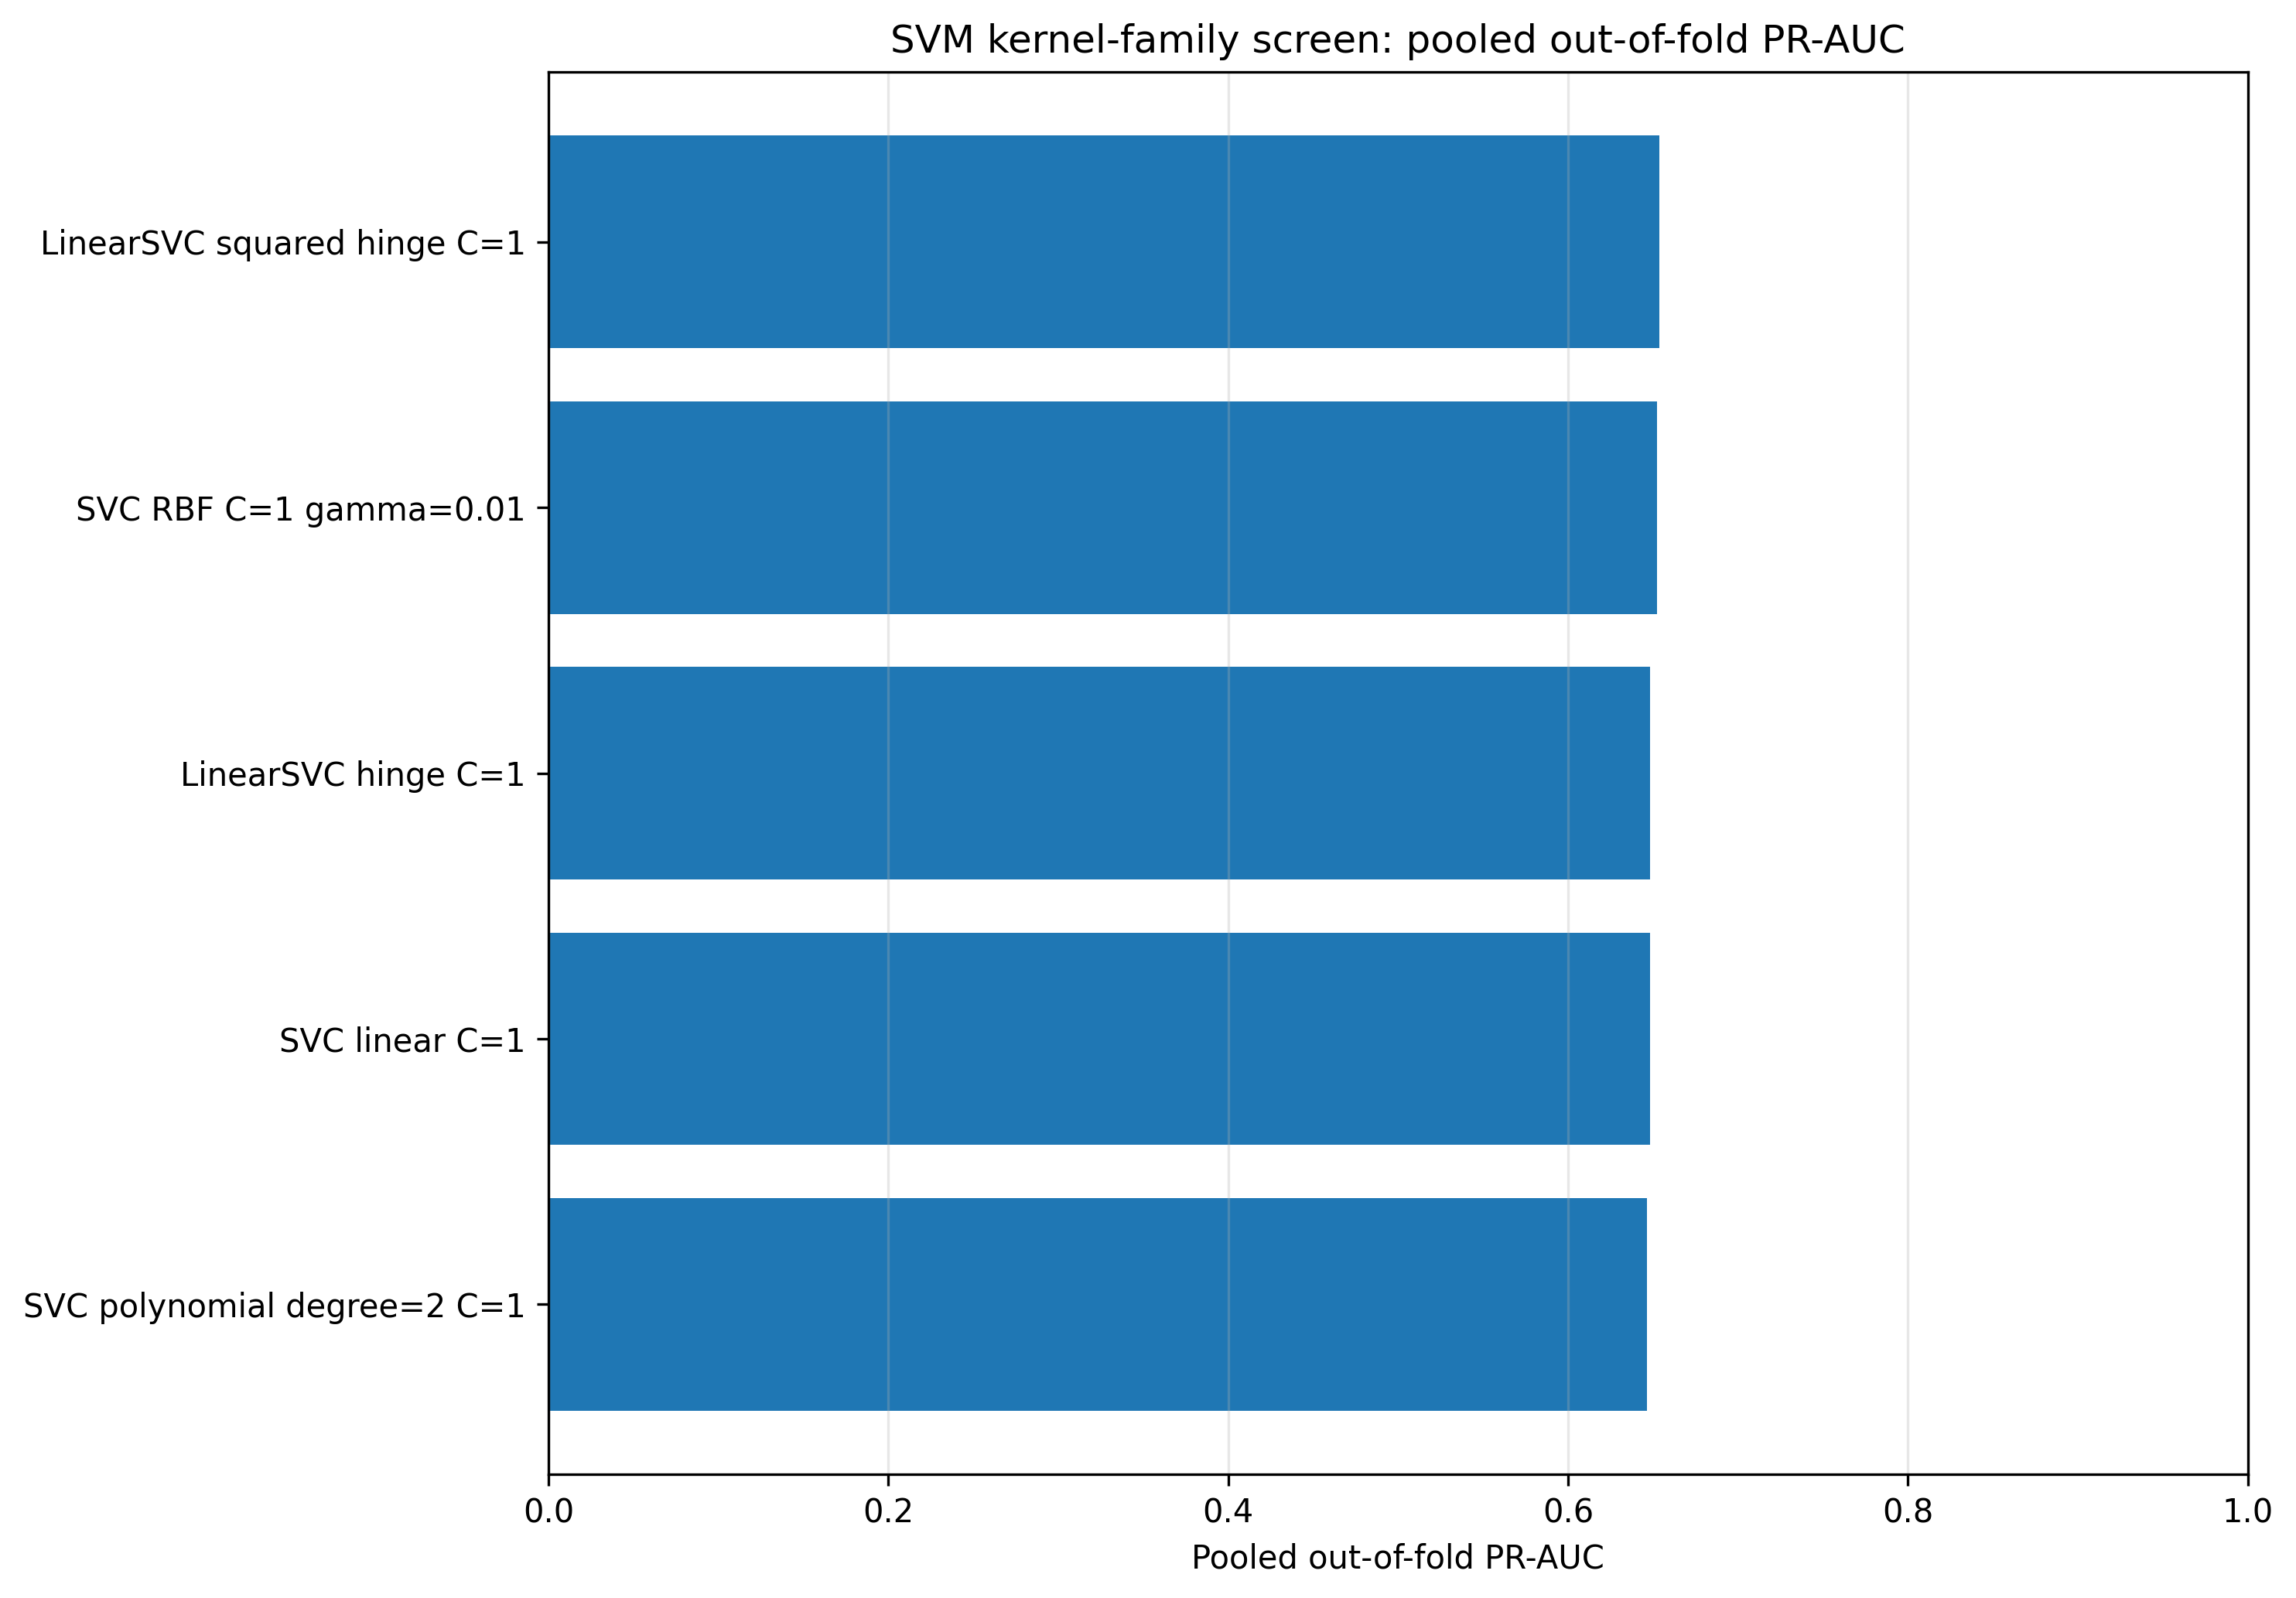
\includegraphics[width=0.88\textwidth]{../figures/svm_kernel_screen_pr_auc.png}
\caption{Kernel-family screen: pooled out-of-fold PR-AUC}
\label{fig:svm-kernel-screen}
\end{figure}

\subsection{Linear SVM fixed grid}

The linear SVM grid varies \(C\), loss function, and class weighting. Table~\ref{tab:svm-linear-grid-summary} presents representative rows from the fixed grid. The strongest observed linear configuration uses squared hinge loss, \(C=0.1\), and \texttt{class\_weight="balanced"}. Its mean fold-level validation PR-AUC is \(0.659\), with mean ROC-AUC \(0.845\), balanced accuracy \(0.765\), and \(F_1\) \(0.627\).

\begin{table}[H]
\centering
\small
\begin{tabular}{llrrrrr}
\toprule
Loss & Class weight & \(C\) & Mean CV PR-AUC & Mean CV ROC-AUC & Bal. Acc. & \(F_1\) \\
\midrule
Squared hinge & balanced & 0.10 & 0.659 & 0.845 & 0.765 & 0.627 \\
Squared hinge & none & 0.10 & 0.657 & 0.843 & 0.715 & 0.587 \\
Hinge & balanced & 0.01 & 0.658 & 0.842 & 0.751 & 0.606 \\
Hinge & none & 0.01 & 0.652 & 0.837 & 0.714 & 0.585 \\
\bottomrule
\end{tabular}
\caption{Representative linear-SVM fixed-grid results using mean fold-level validation metrics}
\label{tab:svm-linear-grid-summary}
\end{table}

The squared-hinge balanced candidates are stable across the tested \(C\) range. Their mean validation PR-AUC remains between approximately \(0.658\) and \(0.659\) for \(C\in\{0.01,0.1,1,10\}\). This is evidence that the linear SVM is not highly sensitive to the tested regularization range. It does not establish that exactly \(C=0.1\) is uniquely optimal.

Class weighting changes the default operating point more strongly than the ranking quality. At \(C=0.1\), enabling balanced weights raises mean recall from \(0.532\) to \(0.807\) and mean balanced accuracy from \(0.715\) to \(0.765\), while mean precision falls from \(0.655\) to \(0.513\). The class-weighted model identifies more potential churners at the natural score boundary, which can be attractive when missed churners are costly.

\begin{figure}[H]
\centering
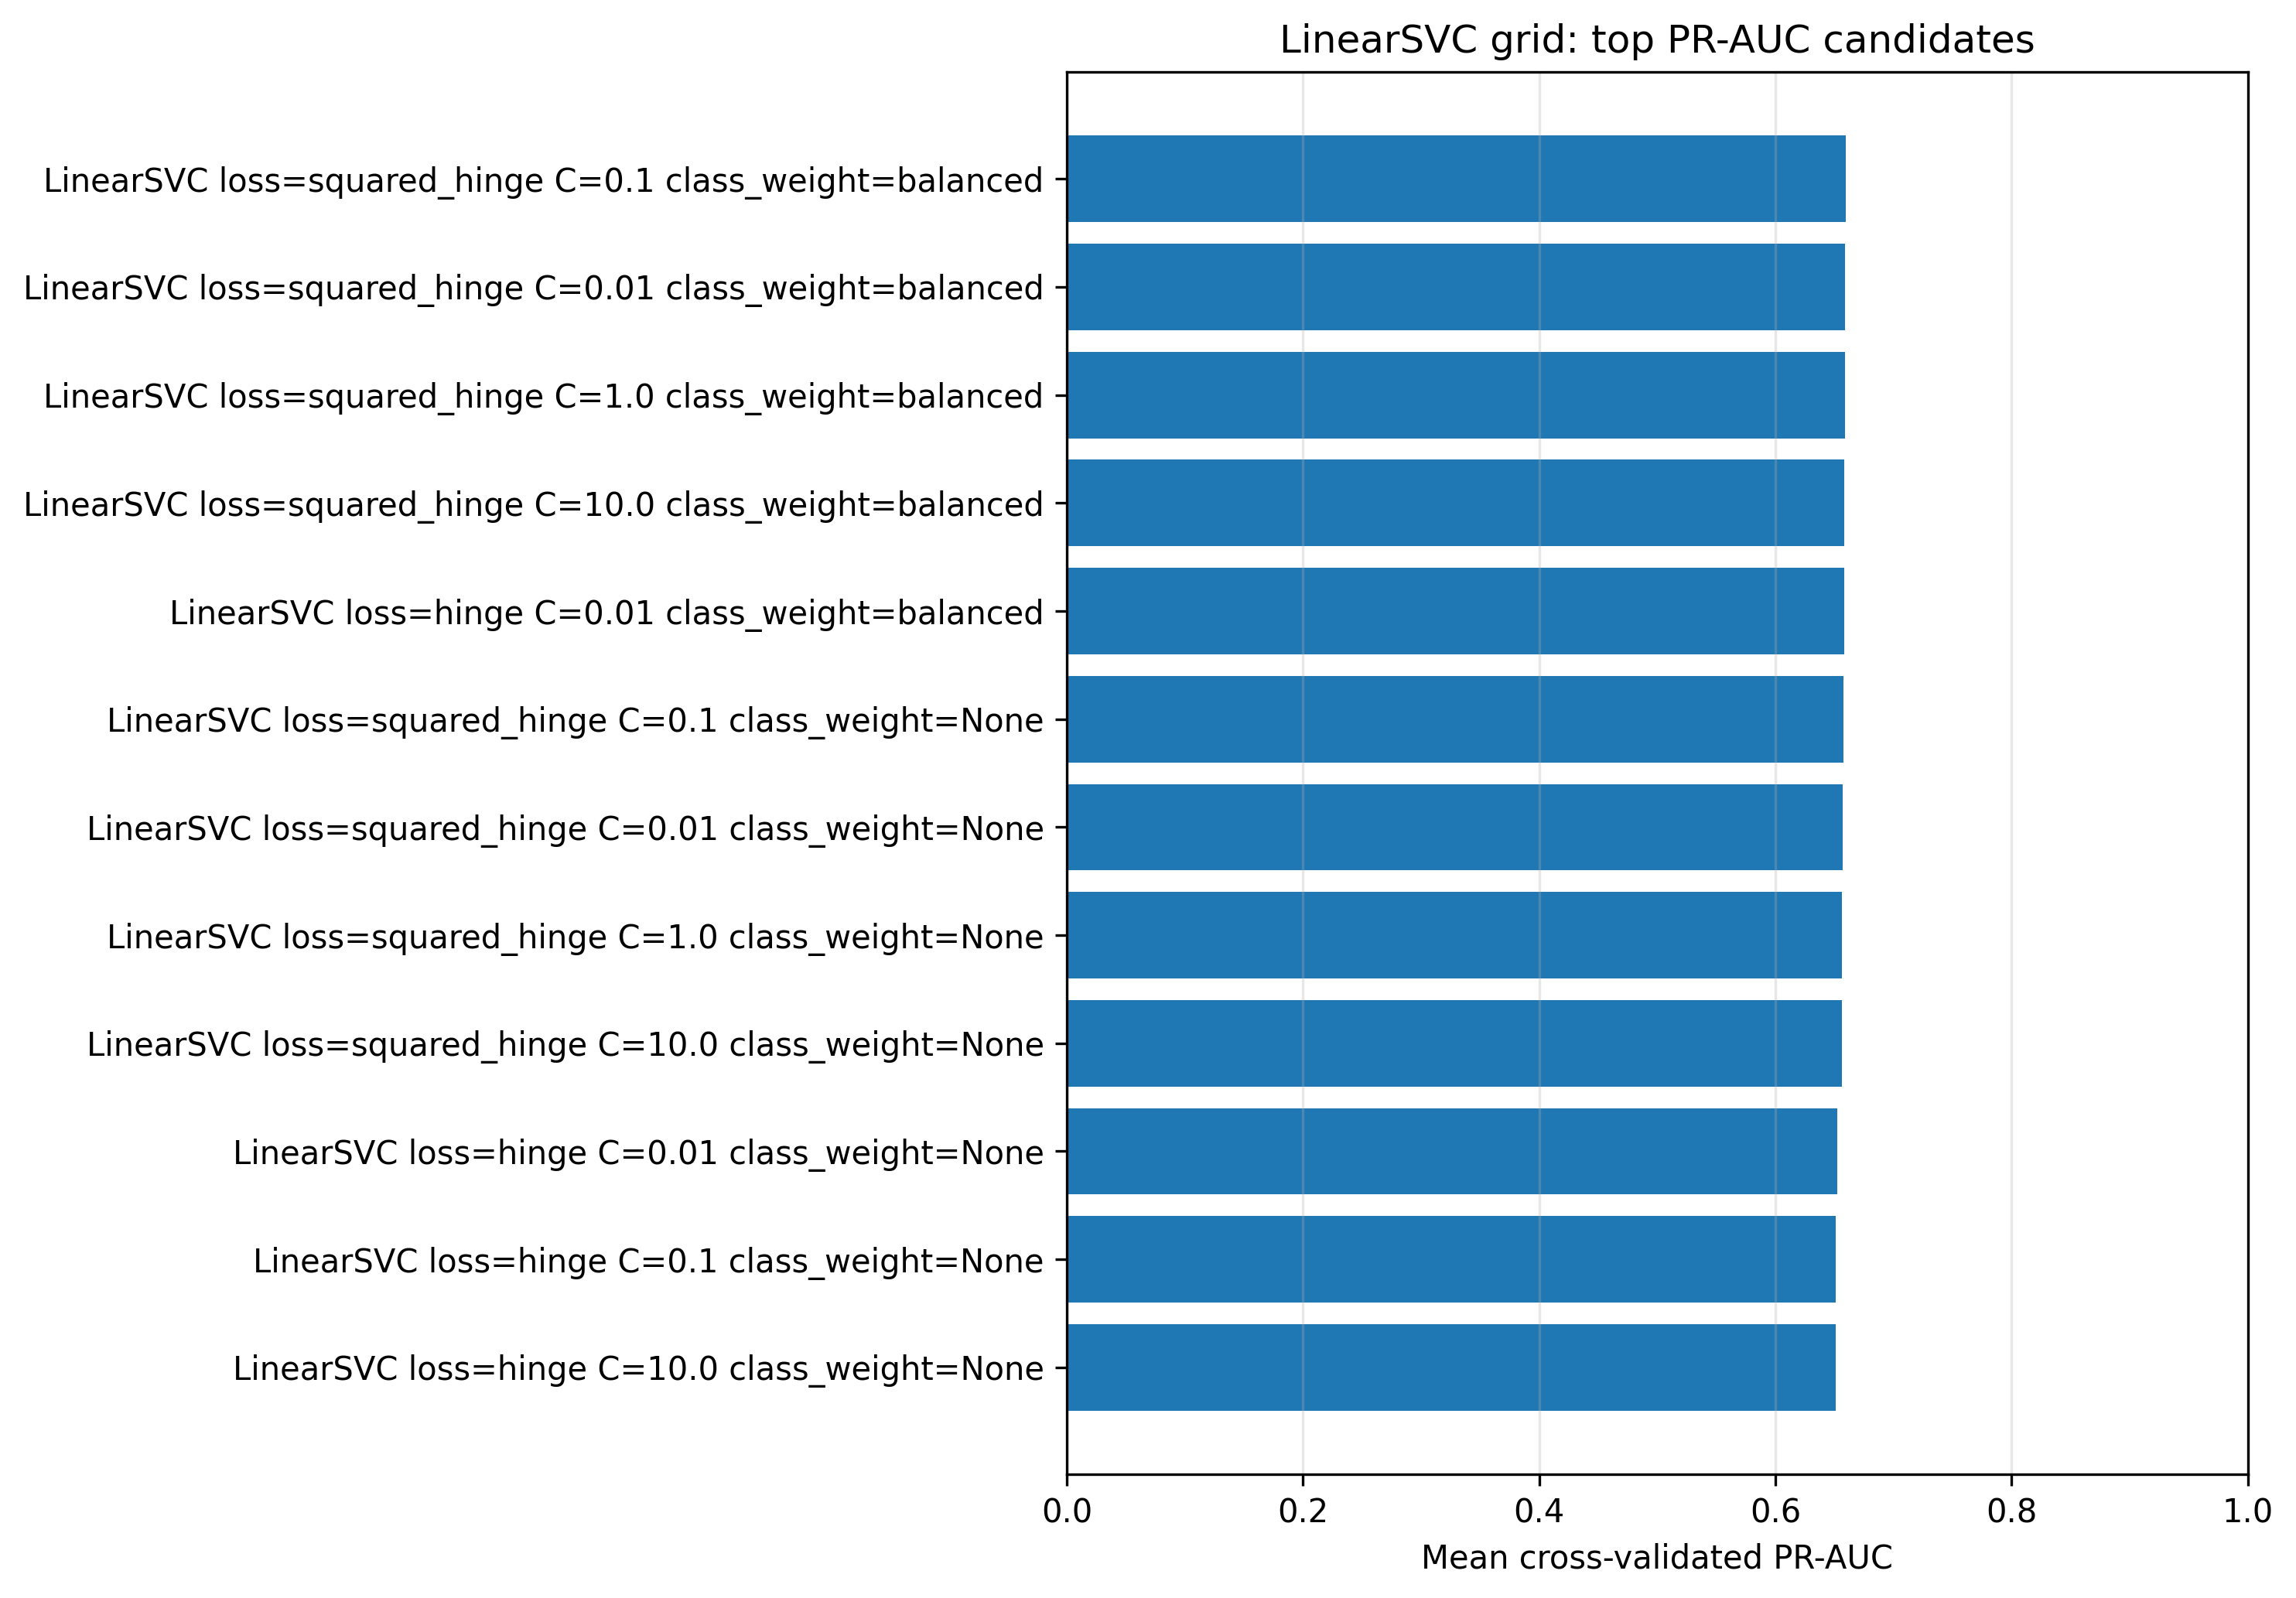
\includegraphics[width=0.88\textwidth]{../figures/svm_linear_grid_pr_auc.png}
\caption{LinearSVC fixed grid: top mean cross-validated PR-AUC candidates}
\label{fig:svm-linear-grid}
\end{figure}

\subsection{RBF-kernel SVM fixed grid}

The RBF grid varies \(C\), \(\gamma\), and class weighting. The strongest observed RBF candidate is
\[
C=10,
\qquad
\gamma=0.001,
\qquad
\texttt{class\_weight="balanced"}.
\]
Its mean fold-level validation PR-AUC is \(0.6595\), only \(0.0001\) above the strongest linear candidate. Table~\ref{tab:svm-rbf-grid-summary} shows representative configurations.

\begin{table}[H]
\centering
\small
\resizebox{\textwidth}{!}{%
\begin{tabular}{rrlrrrr}
\toprule
\(C\) & \(\gamma\) & Class weight & Mean CV PR-AUC & Mean CV ROC-AUC & Train PR-AUC & Fit time (s) \\
\midrule
10.0 & 0.001 & balanced & 0.659 & 0.842 & 0.663 & 0.419 \\
1.0 & 0.010 & balanced & 0.658 & 0.842 & 0.668 & 0.438 \\
0.1 & 0.010 & balanced & 0.655 & 0.840 & 0.657 & 0.442 \\
10.0 & 0.100 & none & 0.572 & 0.773 & 0.857 & 0.464 \\
\bottomrule
\end{tabular}%
}
\caption{Representative RBF-SVC fixed-grid results using mean fold-level validation metrics}
\label{tab:svm-rbf-grid-summary}
\end{table}

The small selected \(\gamma\) value corresponds to a smooth nonlinear boundary. The grid also shows the expected high-variance failure mode at large \(\gamma\). With \(C=10\), \(\gamma=0.1\), and no class weighting, mean training PR-AUC rises to \(0.857\) while mean validation PR-AUC falls to \(0.572\). This large train-validation gap indicates that a very local RBF boundary can fit fold-specific structure without improving unseen churn ranking.

The selected RBF candidate requires substantially more computation than the selected linear candidate. Mean per-fold fit time is approximately \(0.419\) seconds for the selected RBF SVC versus approximately \(0.039\) seconds for the selected LinearSVC. The difference is not prohibitive for this dataset, but it matters when the nonlinear model does not provide a clear ranking improvement.

\begin{figure}[H]
\centering
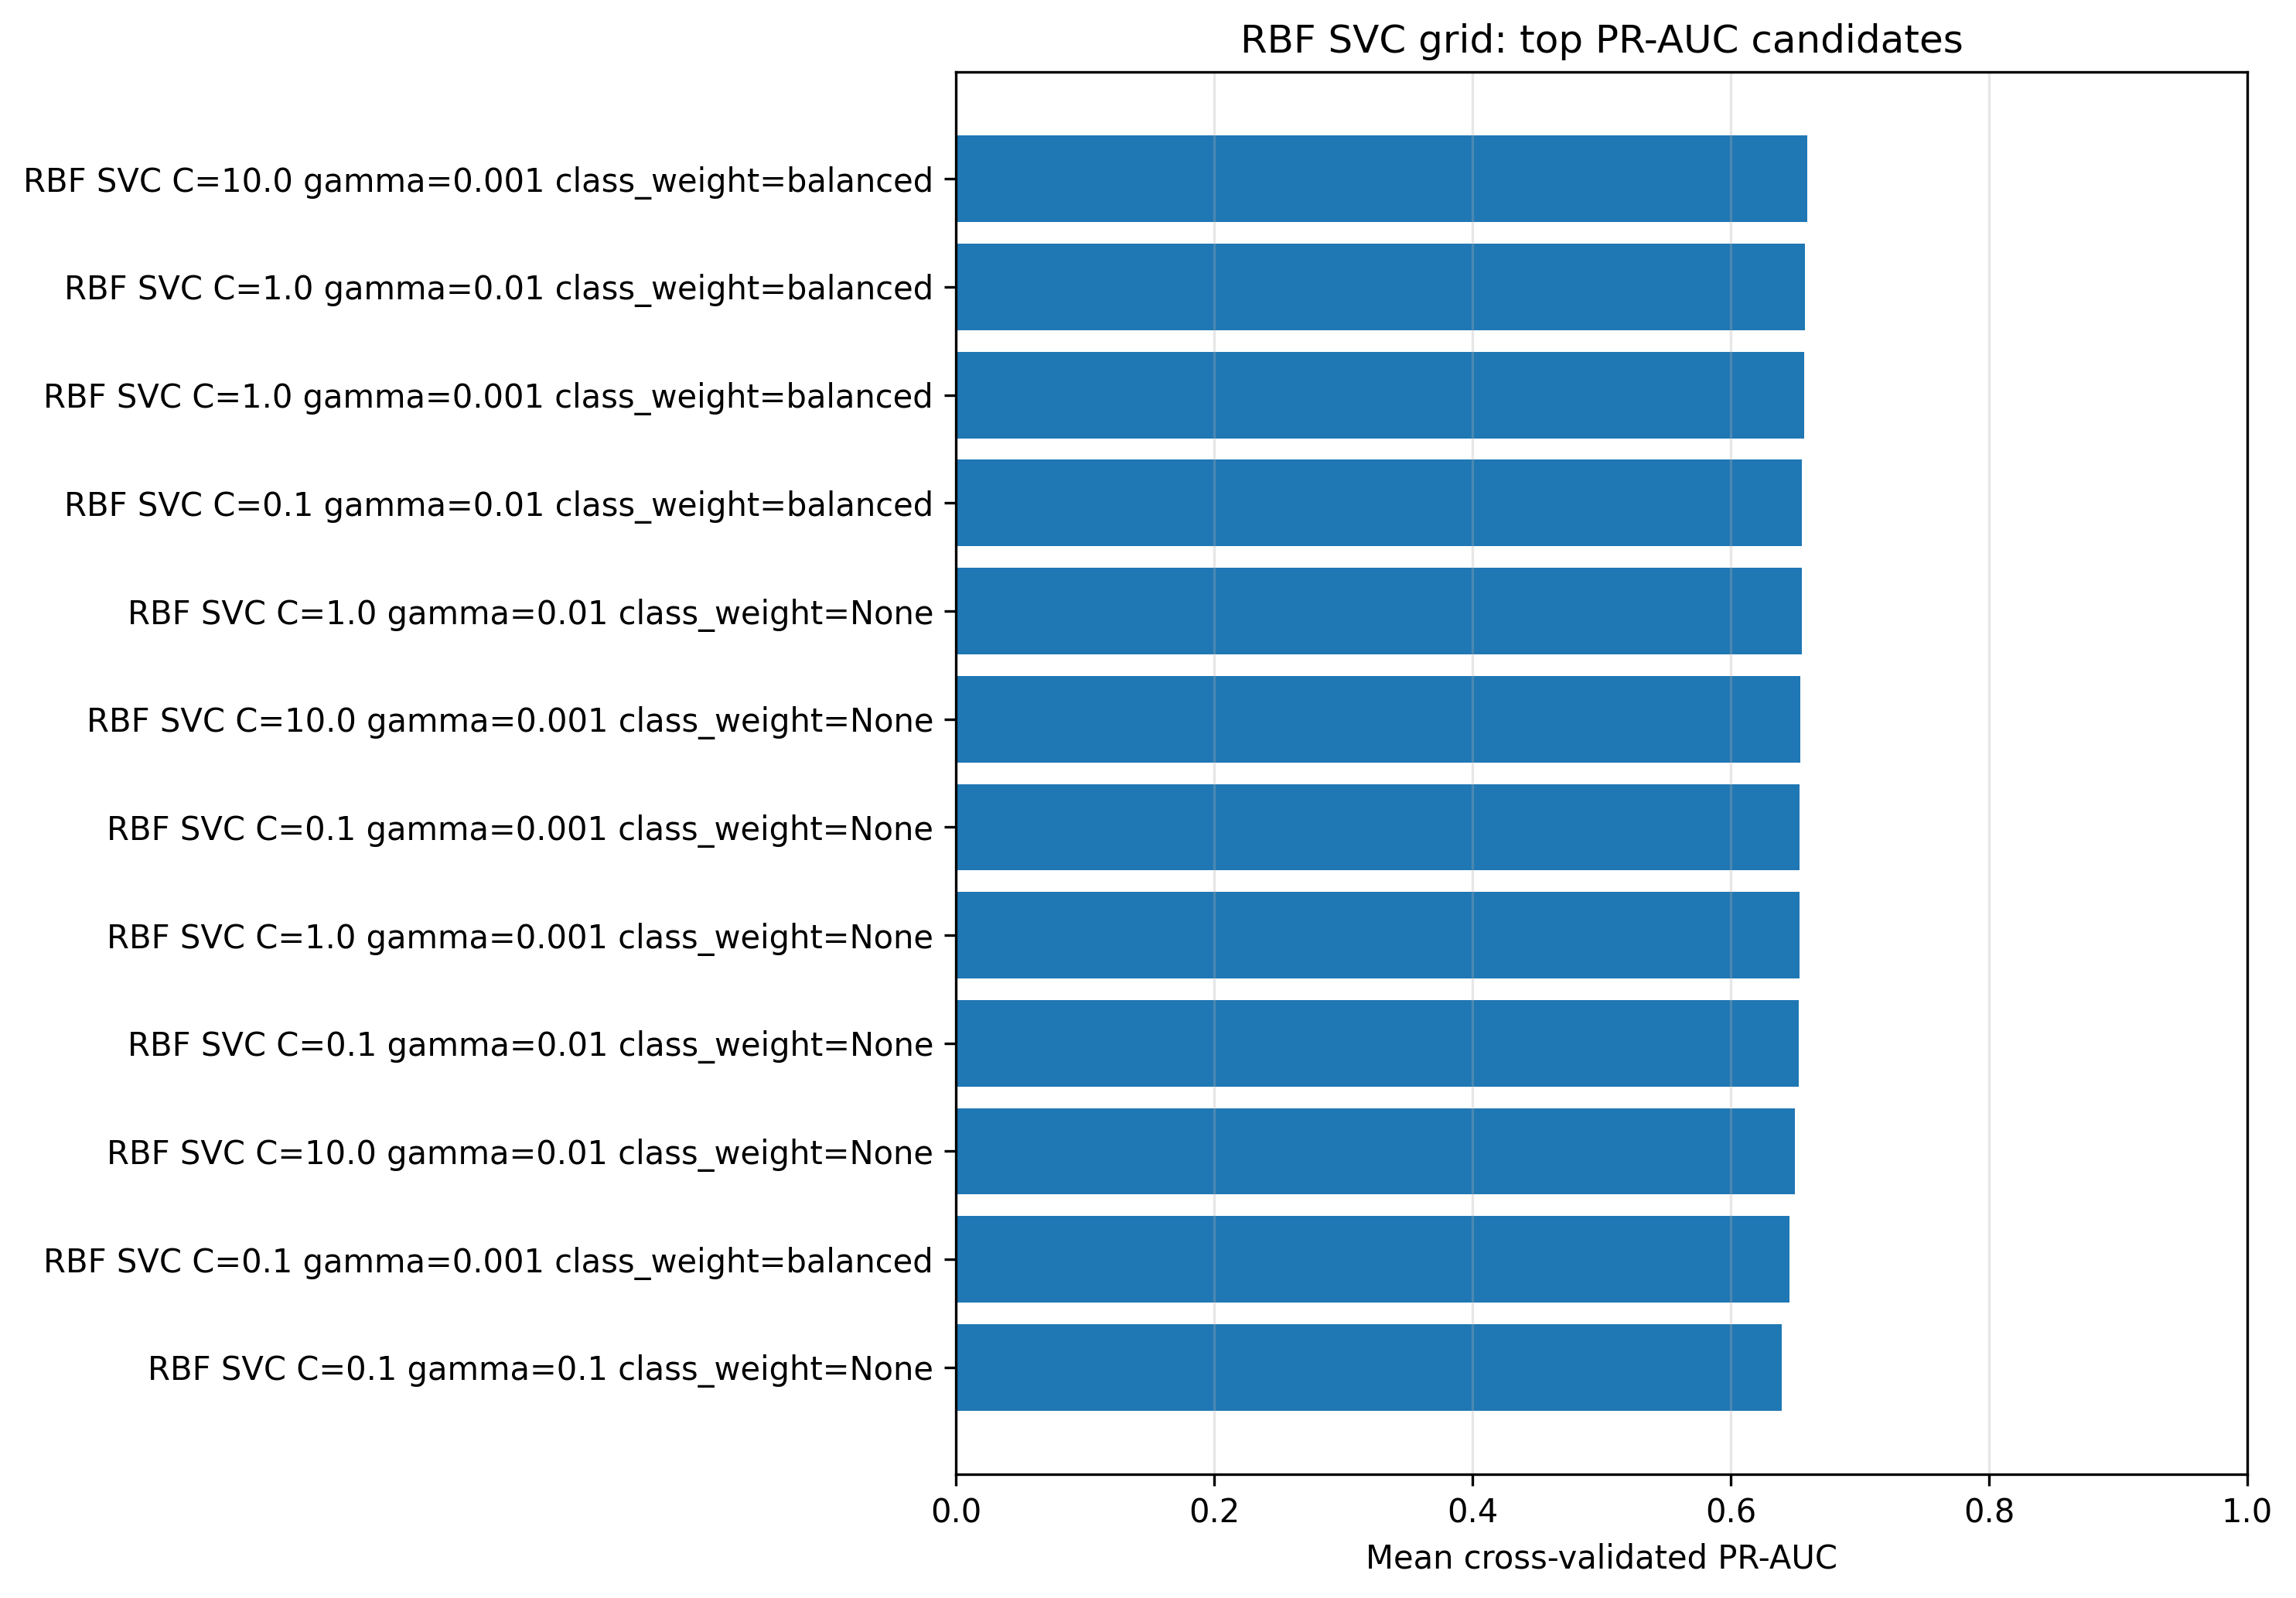
\includegraphics[width=0.88\textwidth]{../figures/svm_rbf_grid_pr_auc.png}
\caption{RBF-SVC fixed grid: top mean cross-validated PR-AUC candidates}
\label{fig:svm-rbf-grid}
\end{figure}

\subsection{Selected linear and RBF candidates}

Table~\ref{tab:svm-selected-family-candidates} summarizes the selected candidate from each SVM family. The fixed-grid family-selection rule is mean fold-level validation PR-AUC, followed by balanced accuracy and \(F_1\). The RBF candidate has a numerically larger PR-AUC by only \(0.0001\), far below the observed fold-to-fold standard deviations of \(0.016\) to \(0.018\). The appropriate conclusion is that the selected linear and RBF candidates are effectively tied within this development grid.

\begin{table}[H]
\centering
\small
\resizebox{\textwidth}{!}{%
\begin{tabular}{llrrrr}
\toprule
Family & Selected configuration & Mean CV PR-AUC & Mean CV ROC-AUC & Bal. Acc. & \(F_1\) \\
\midrule
LinearSVC & squared hinge, \(C=0.1\), balanced & 0.6594 & 0.8453 & 0.7648 & 0.6267 \\
RBF SVC & \(C=10\), \(\gamma=0.001\), balanced & 0.6595 & 0.8424 & 0.7464 & 0.6003 \\
\bottomrule
\end{tabular}%
}
\caption{Selected linear and RBF SVM candidates from the fixed development grids}
\label{tab:svm-selected-family-candidates}
\end{table}

The subsequent pooled out-of-fold diagnostic produces a different ordering. The selected linear model has pooled OOF PR-AUC \(0.6565\), whereas the selected RBF model has \(0.6426\). This is not a contradiction. Mean fold-level PR-AUC and PR-AUC calculated after concatenating all out-of-fold scores are different statistics. PR-AUC is nonlinear, and the raw decision-score scales of separately fitted SVMs can differ across folds. The pre-specified mean fold-level statistic remains the appropriate grid-selection criterion. The pooled diagnostic is used for descriptive curves, confusion matrices, and a common within-section comparison.

Taken together, the results justify retaining the linear SVM as the representative SVM for detailed diagnostics. It is essentially tied with RBF in the selected grid, is materially faster, yields directly interpretable coefficient directions, and has the stronger pooled OOF diagnostic. This does not prove that linear SVM is globally superior to RBF SVM.

\subsection{Scoped comparison with selected reference models}

For this section, the selected SVM candidates are compared with representative models from earlier sections. The earlier model rows are not copied from stored result CSV files. Each selected configuration is reconstructed from its previously selected hyperparameters and re-evaluated through fresh training-only cross-validation in the SVM notebook. This supplies comparable pooled out-of-fold predictions, metrics, and confusion matrices under the same current evaluation procedure.

The comparison is deliberately scoped. It includes logistic regression, kNN, a single tree, bagging, random forest, and a strong XGBoost reference. It does not include every selected boosting implementation, such as CatBoost, LightGBM, or \texttt{GradientBoostingClassifier}. Therefore, Table~\ref{tab:svm-model-comparison} is a section-level diagnostic, not the final project-wide model ranking.

\begin{table}[H]
\centering
\small
\resizebox{\textwidth}{!}{
\begin{tabular}{lrrrrrrrr}
\toprule
Model & Accuracy & Bal. Acc. & Precision & Recall & Specificity & \(F_1\) & ROC-AUC & PR-AUC \\
\midrule
Best XGBoost reference & 0.808 & 0.722 & 0.671 & 0.539 & 0.905 & 0.598 & 0.850 & 0.670 \\
Selected bagged trees & 0.800 & 0.705 & 0.662 & 0.504 & 0.907 & 0.572 & 0.846 & 0.662 \\
Selected random forest & 0.804 & 0.706 & 0.678 & 0.498 & 0.914 & 0.574 & 0.847 & 0.660 \\
Selected L2 logistic regression & 0.802 & 0.719 & 0.652 & 0.544 & 0.895 & 0.593 & 0.846 & 0.658 \\
Selected LinearSVC & 0.745 & 0.765 & 0.513 & 0.807 & 0.723 & 0.627 & 0.845 & 0.657 \\
Selected RBF SVC & 0.706 & 0.746 & 0.469 & 0.833 & 0.659 & 0.600 & 0.838 & 0.643 \\
Selected single decision tree & 0.789 & 0.701 & 0.624 & 0.514 & 0.888 & 0.564 & 0.824 & 0.628 \\
Selected kNN & 0.792 & 0.722 & 0.617 & 0.571 & 0.872 & 0.593 & 0.836 & 0.628 \\
\bottomrule
\end{tabular}
}
\caption{Scoped pooled out-of-fold comparison of selected SVMs and reconstructed reference models}
\label{tab:svm-model-comparison}
\end{table}

The selected linear SVM is competitive with L2 logistic regression, bagging, and random forests in ranking performance, but it does not surpass the strong XGBoost reference in this scoped comparison. Its default operating point is notably less conservative. It detects many more churners, but also flags more non-churners. Thus, the SVM result reinforces the distinction between ranking quality and the practical threshold policy used to decide which customers receive intervention.

\begin{figure}[H]
\centering
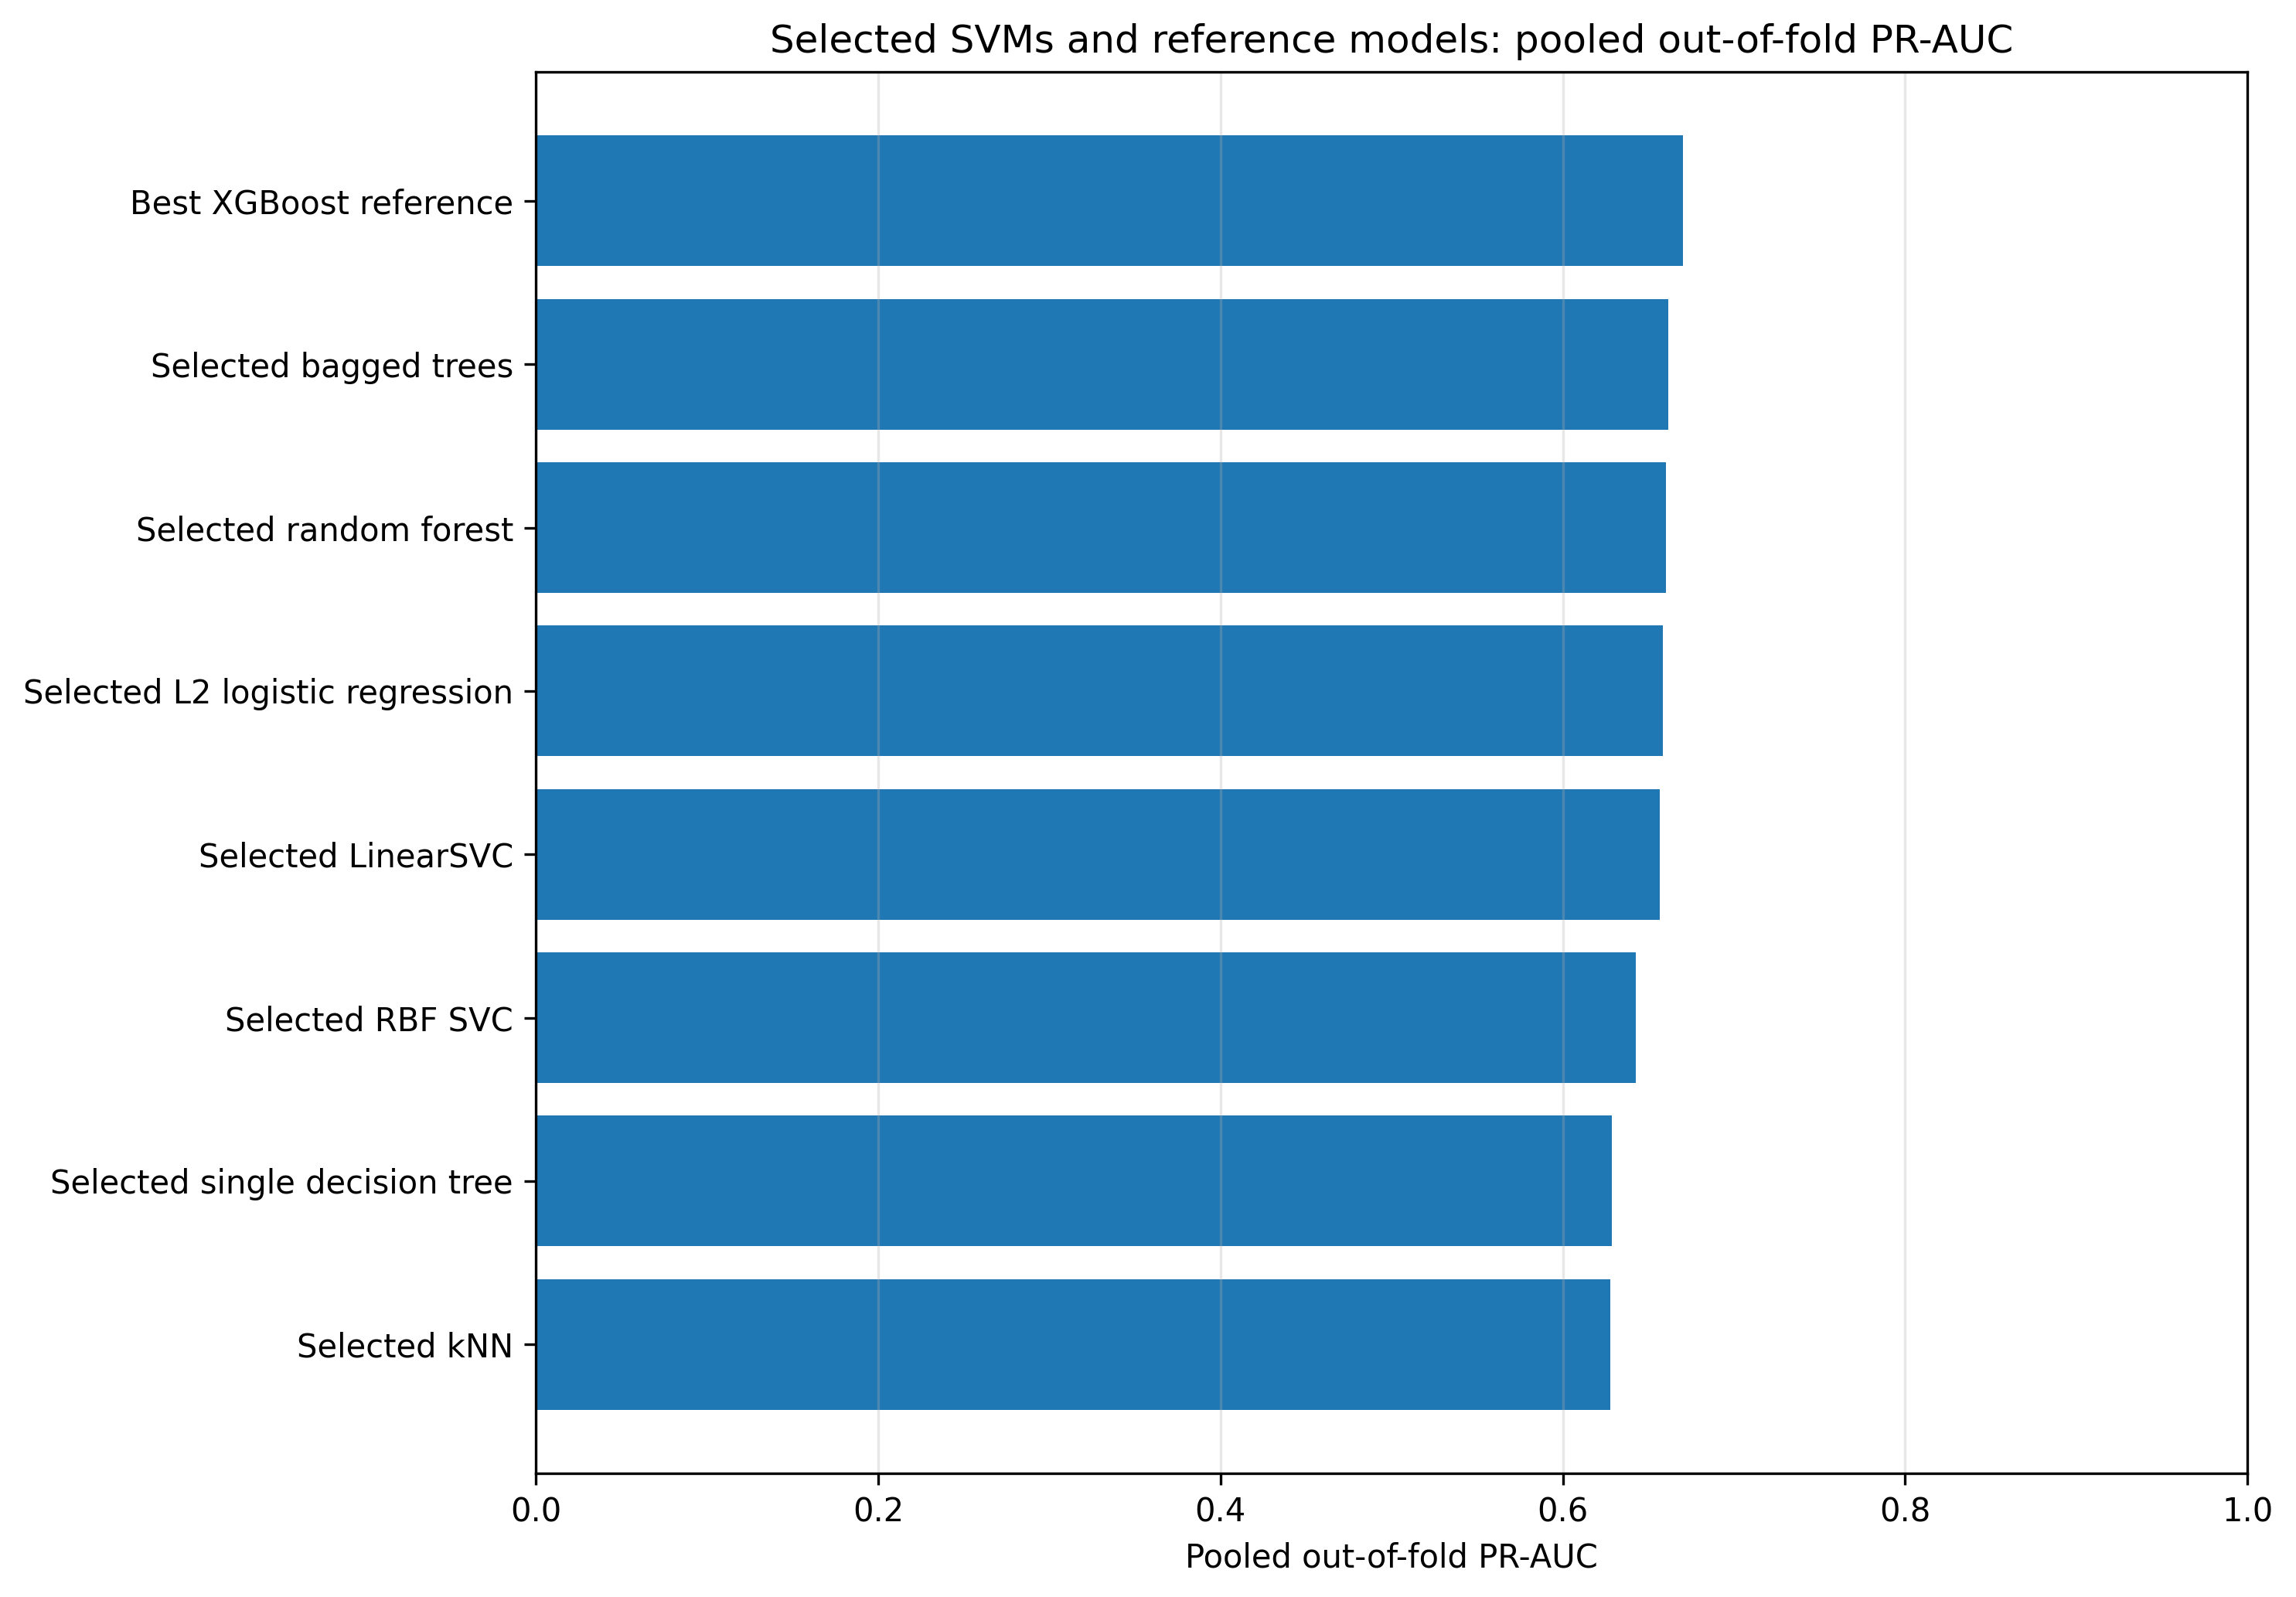
\includegraphics[width=0.88\textwidth]{../figures/svm_model_comparison_pr_auc.png}
\caption{Selected SVMs and scoped reference models: pooled out-of-fold PR-AUC}
\label{fig:svm-model-comparison}
\end{figure}

\subsection{Default-boundary confusion-matrix behaviour}

The selected SVM candidates use the class-weighted default score boundary. Table~\ref{tab:svm-confusion} shows positive-first pooled out-of-fold counts. The selected linear SVM detects \(1206\) of the \(1495\) churners, corresponding to recall \(0.807\), but also produces \(1147\) false positives. The selected RBF SVM detects \(1246\) churners and produces \(1410\) false positives.

\begin{table}[H]
\centering
\small
\begin{tabular}{lrrrrr}
\toprule
Model & TP & FN & FP & TN & Pred. positive rate \\
\midrule
Selected LinearSVC & 1206 & 289 & 1147 & 2992 & 0.418 \\
Selected RBF SVC & 1246 & 249 & 1410 & 2729 & 0.471 \\
Selected L2 logistic regression & 813 & 682 & 434 & 3705 & 0.221 \\
Best XGBoost reference & 806 & 689 & 395 & 3744 & 0.213 \\
\bottomrule
\end{tabular}
\caption{Positive-first pooled out-of-fold confusion-matrix counts for selected SVMs and compact reference models}
\label{tab:svm-confusion}
\end{table}

This default-boundary behaviour follows directly from class weighting. The selected LinearSVC flags approximately \(41.8\%\) of customers as potential churners, compared with an observed churn rate of \(26.5\%\). The classifier therefore prioritizes churn recovery rather than a narrow high-precision intervention list. Whether this is preferable depends on retention capacity and the relative costs of false negatives and false positives.

\subsection{Margin-score threshold behaviour}

The selected linear SVM uses a signed decision score, not a predicted probability. Score \(0\) is the natural SVM boundary. Table~\ref{tab:svm-thresholds} reports selected score thresholds. Lower score thresholds increase recall and reduce precision and specificity. Higher thresholds create a more selective intervention list.

\begin{table}[H]
\centering
\small
\begin{tabular}{rrrrrr}
\toprule
Score threshold & Precision & Recall & Specificity & \(F_1\) & Pred. positive rate \\
\midrule
-0.850 & 0.327 & 0.985 & 0.267 & 0.491 & 0.800 \\
-0.304 & 0.426 & 0.924 & 0.551 & 0.583 & 0.575 \\
0.000 & 0.513 & 0.807 & 0.723 & 0.627 & 0.418 \\
0.135 & 0.561 & 0.740 & 0.791 & 0.638 & 0.350 \\
0.291 & 0.610 & 0.633 & 0.854 & 0.621 & 0.275 \\
0.455 & 0.671 & 0.506 & 0.910 & 0.577 & 0.200 \\
\bottomrule
\end{tabular}
\caption{Margin-score threshold behaviour for the selected LinearSVC using pooled out-of-fold scores}
\label{tab:svm-thresholds}
\end{table}

At the natural score threshold \(0\), the selected linear SVM has precision \(0.513\), recall \(0.807\), specificity \(0.723\), and \(F_1\) \(0.627\). Raising the score threshold to approximately \(0.135\) increases the displayed \(F_1\) to \(0.638\), while lowering recall to \(0.740\). Raising it further to approximately \(0.455\) increases precision to \(0.671\), but recall falls to \(0.506\).

These values should not be used to select a final production threshold in this section. The decision scores are uncalibrated margins, not churn probabilities. A later finalist workflow must connect threshold selection to intervention value, contact capacity, and the relative cost of false negatives and false positives. If probability interpretation becomes necessary, calibration should be assessed as a dedicated training-only step.

\begin{figure}[H]
\centering
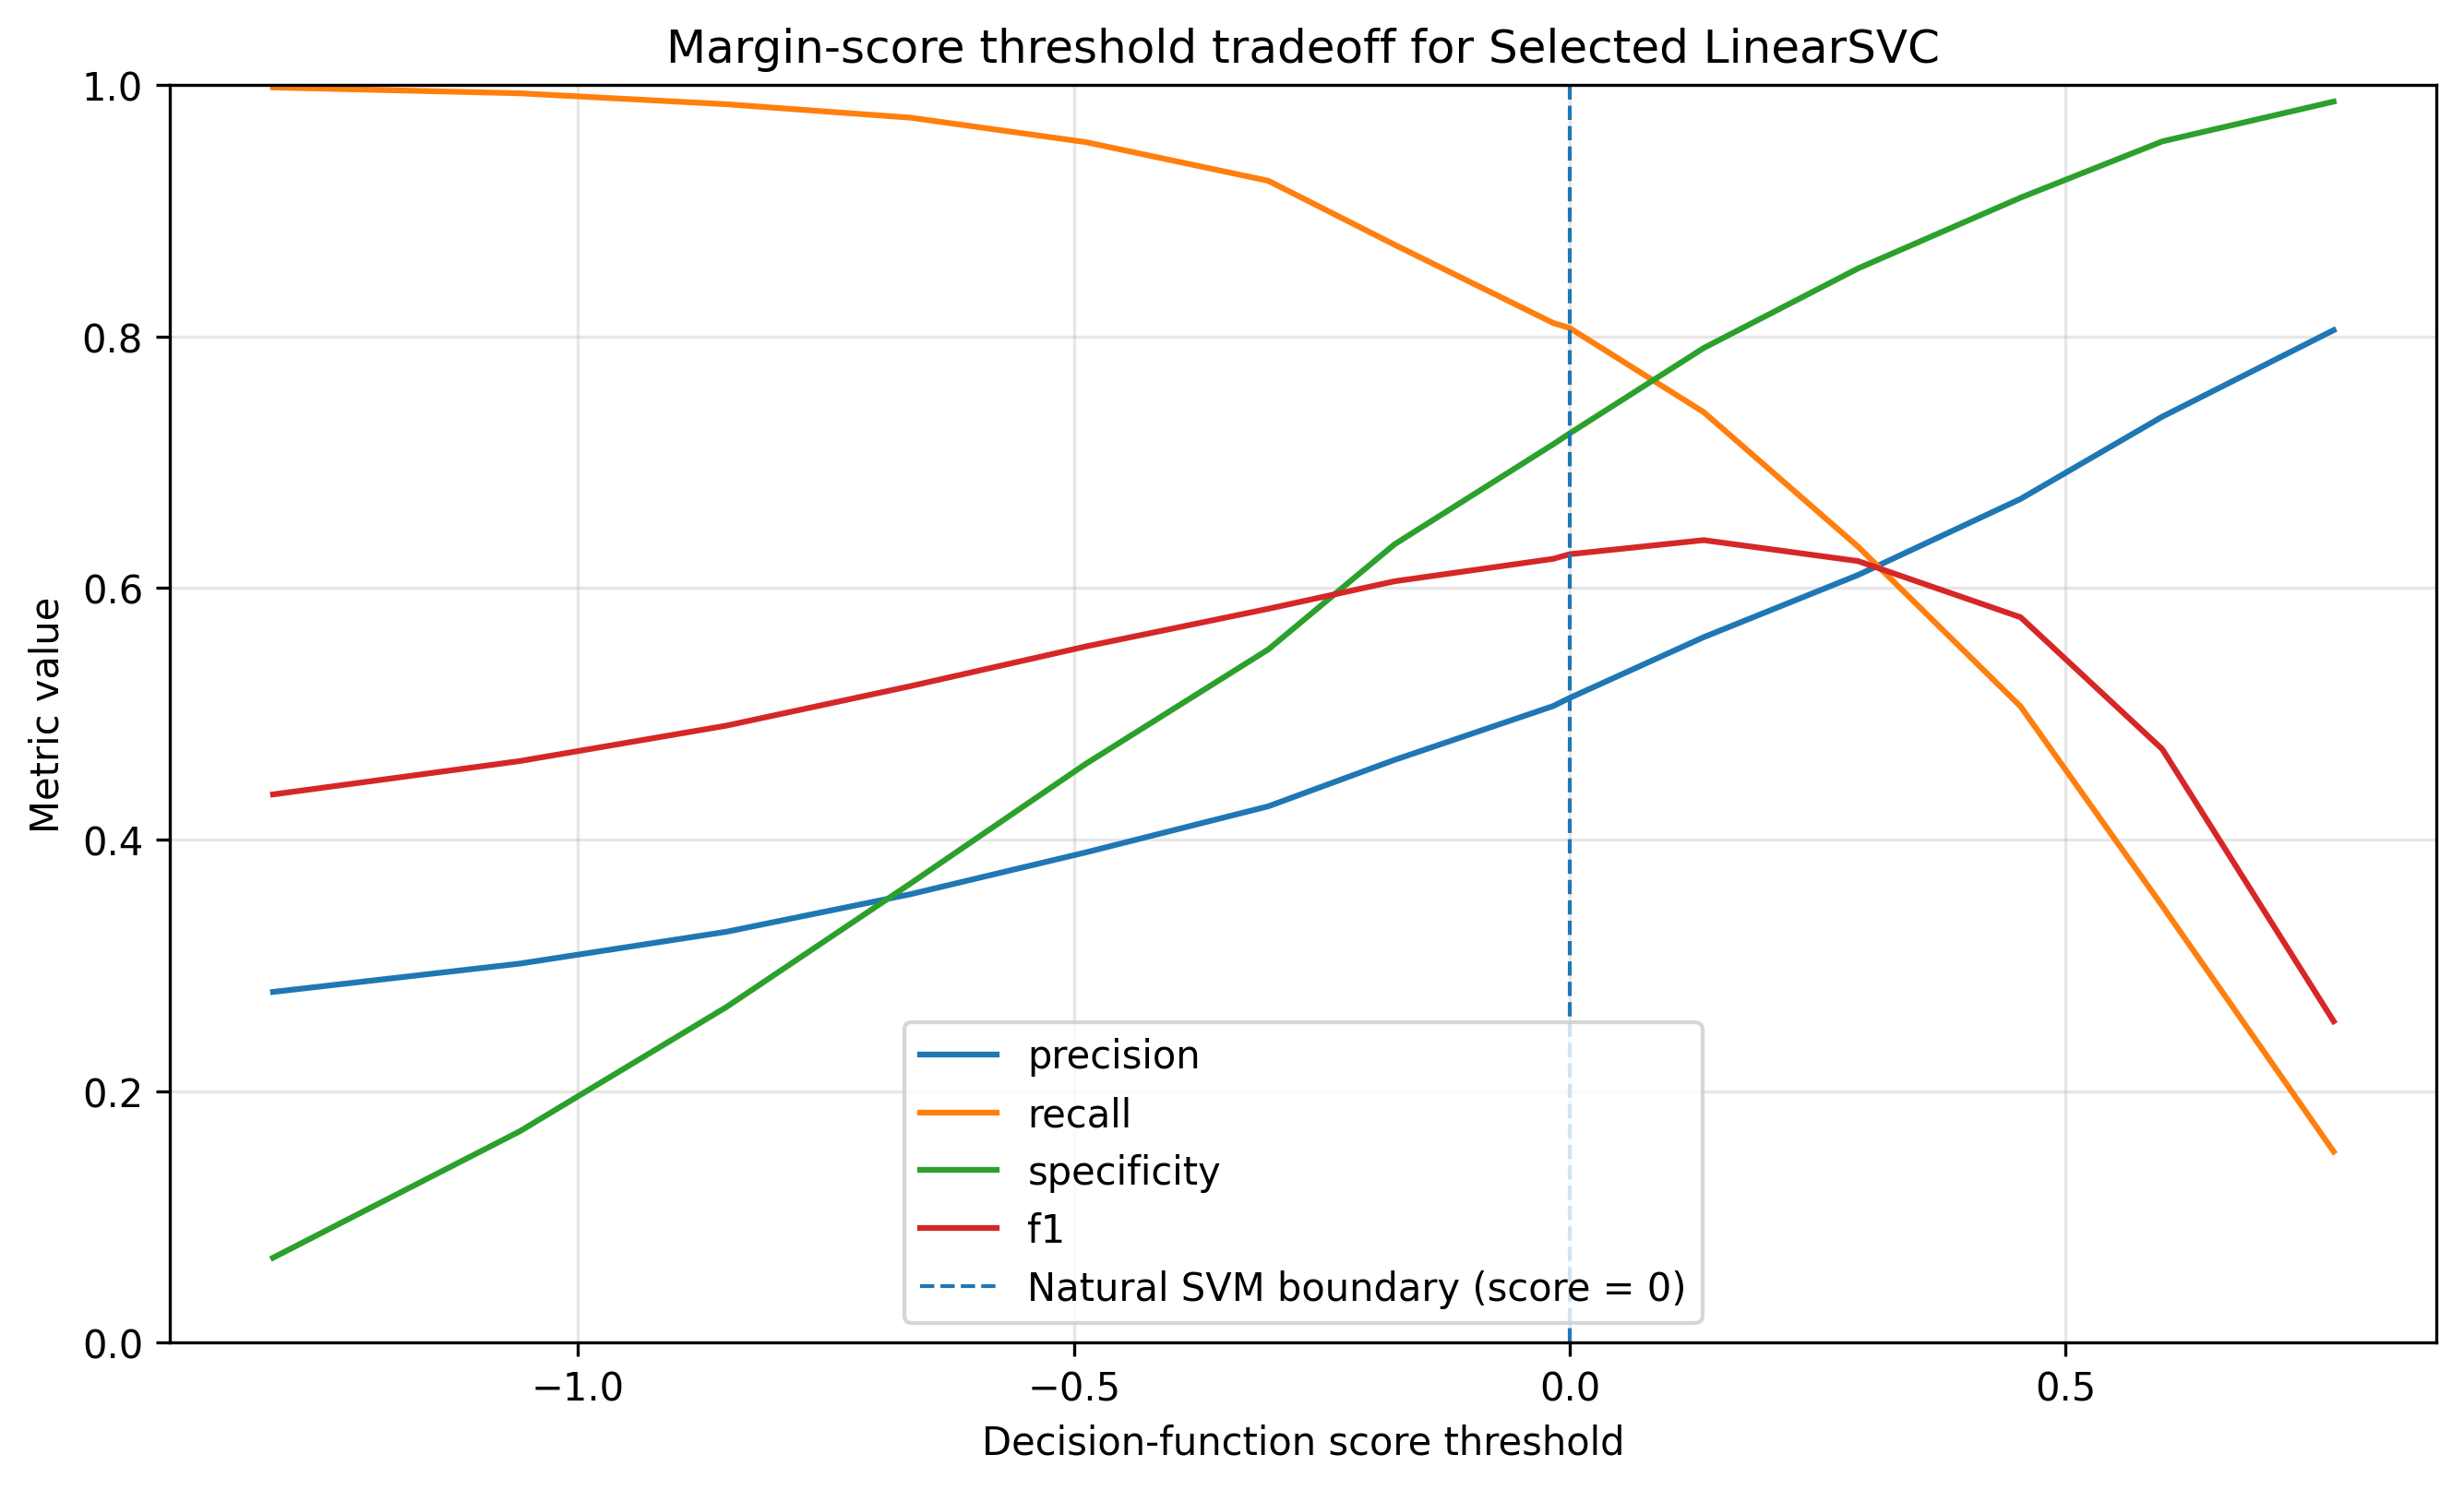
\includegraphics[width=0.88\textwidth]{../figures/svm_margin_score_threshold_tradeoff.png}
\caption{Margin-score threshold tradeoff for the selected LinearSVC}
\label{fig:svm-threshold-tradeoff}
\end{figure}

\subsection{Ranking curves}

Figures~\ref{fig:svm-roc-curve} and~\ref{fig:svm-pr-curve} show the ranking curves for the selected linear SVM. Its pooled OOF ROC-AUC is approximately \(0.845\), while PR-AUC is approximately \(0.657\). The precision-recall curve remains materially above the positive-rate baseline of approximately \(0.265\), indicating that the linear SVM produces useful churn-risk ordering despite the absence of calibrated probabilities.

\begin{figure}[H]
\centering
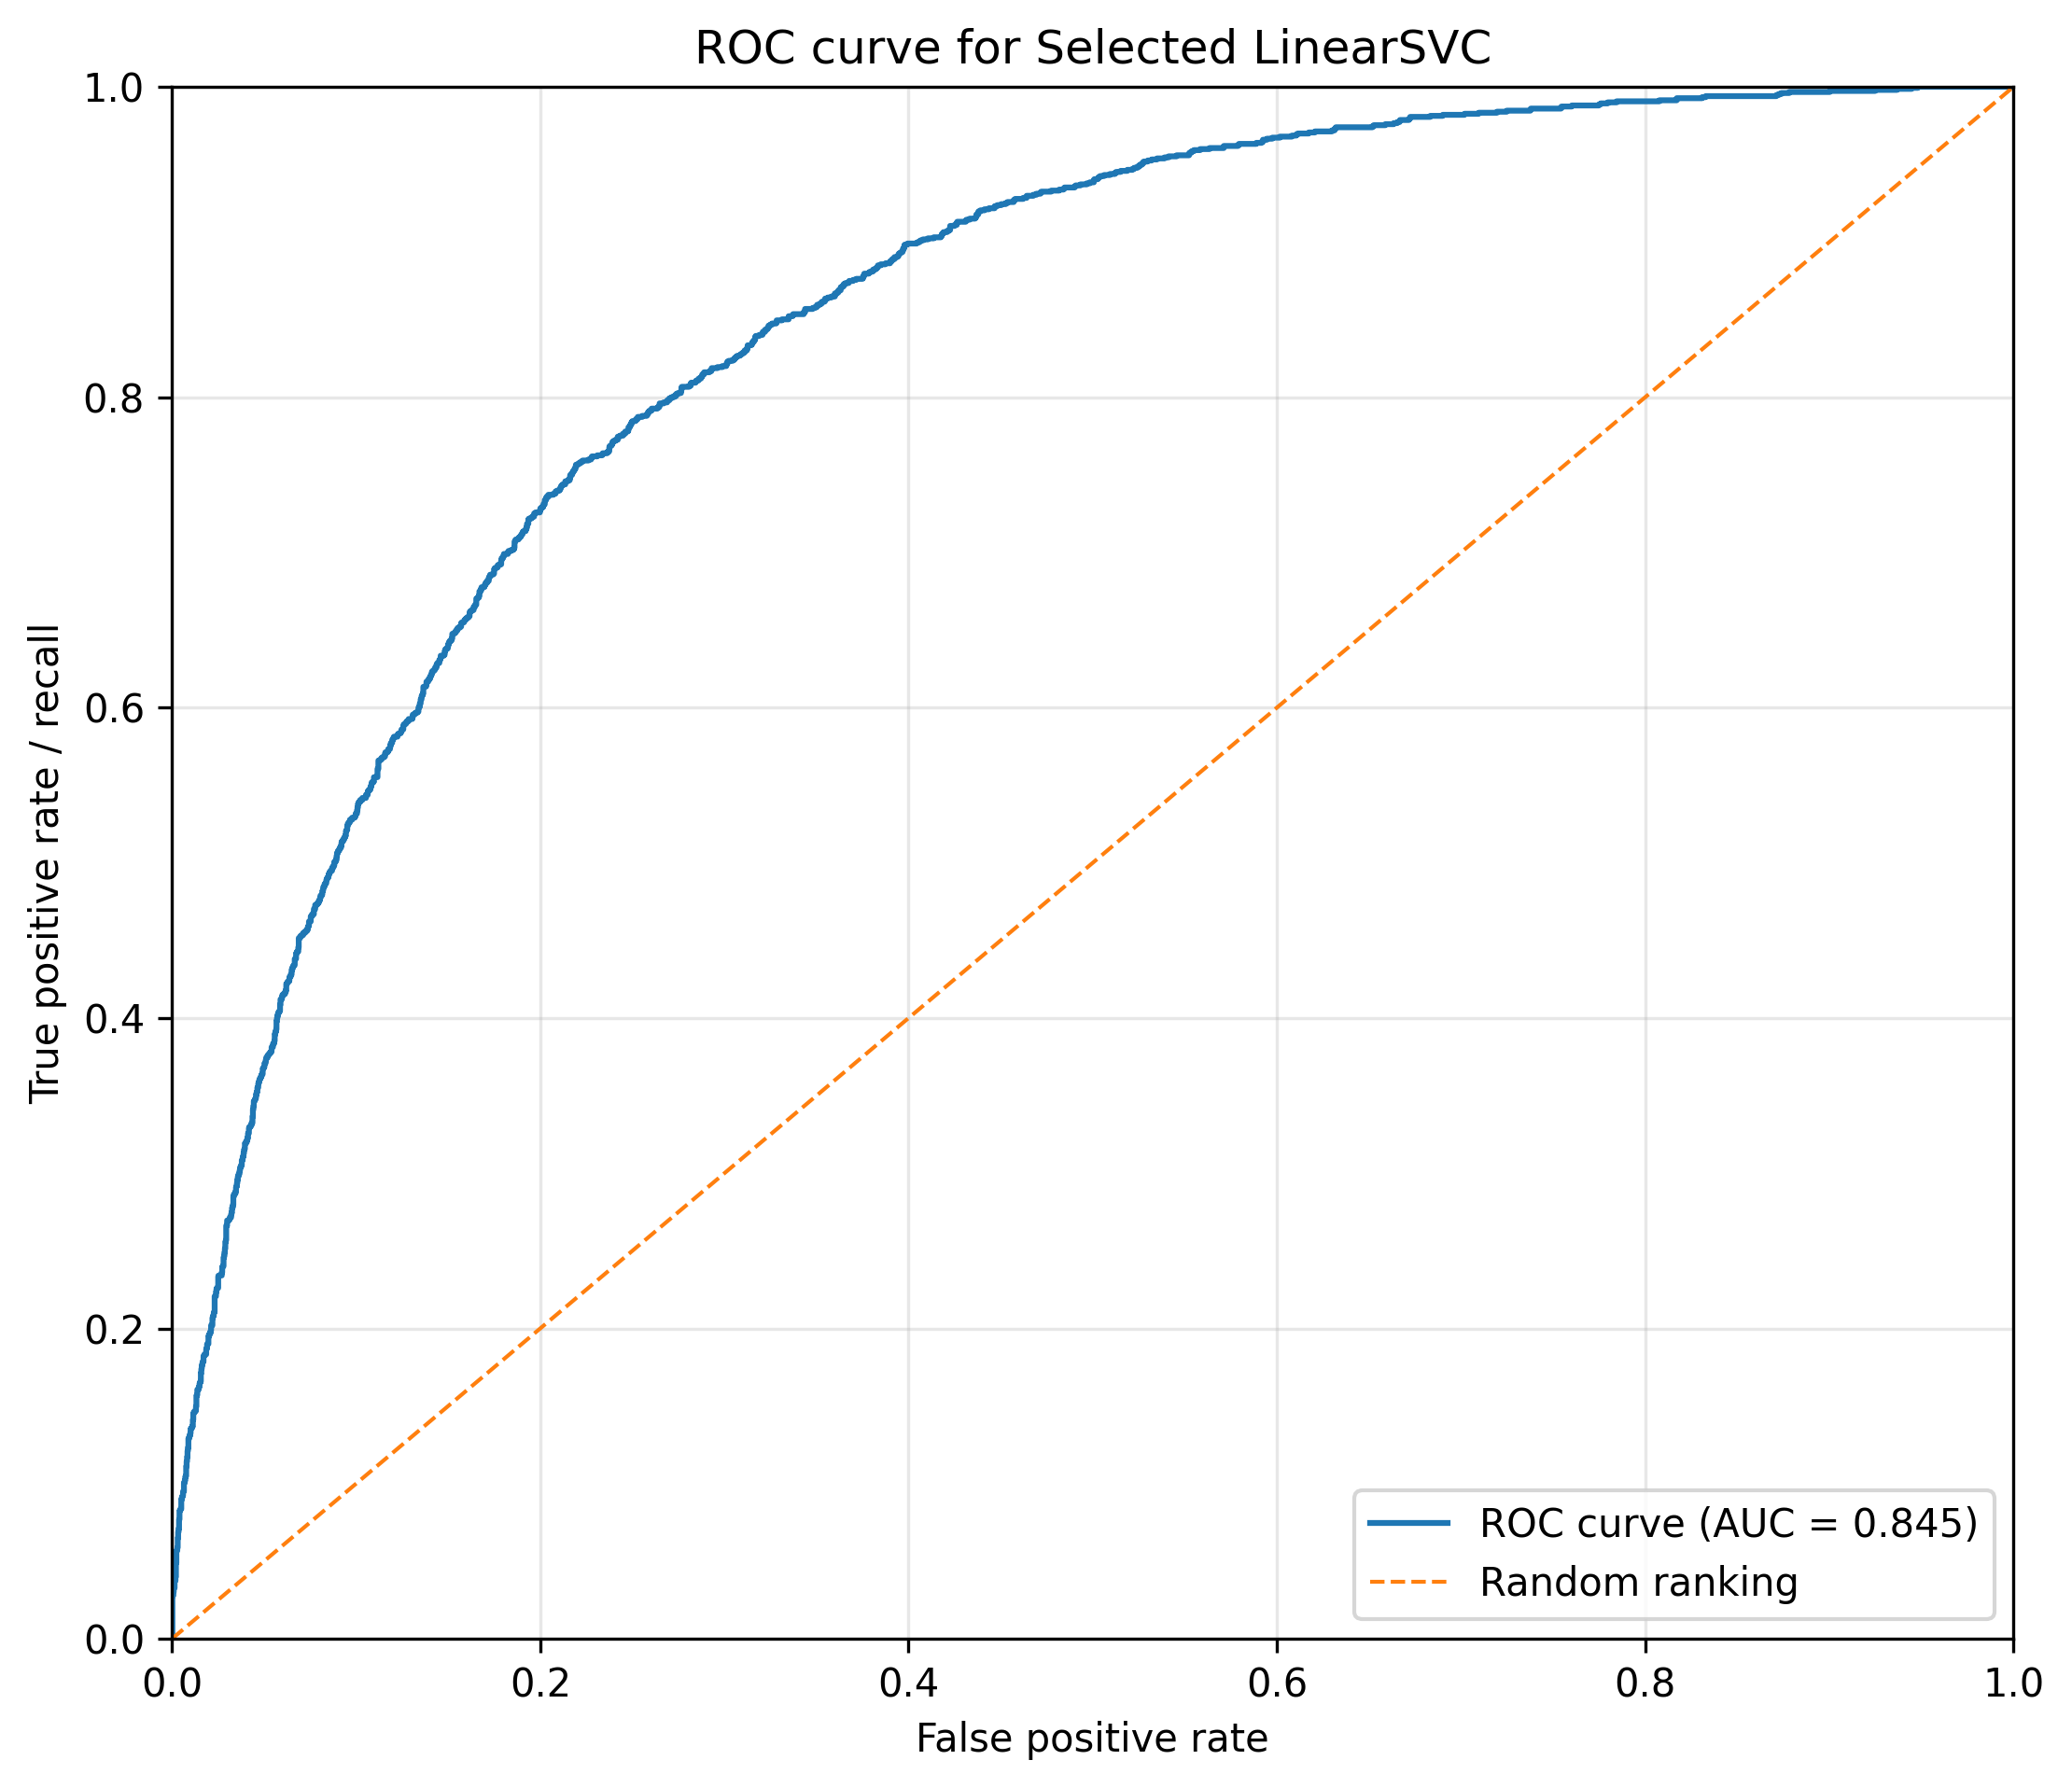
\includegraphics[width=0.82\textwidth]{../figures/svm_roc_curve.png}
\caption{ROC curve for the selected LinearSVC}
\label{fig:svm-roc-curve}
\end{figure}

\begin{figure}[H]
\centering
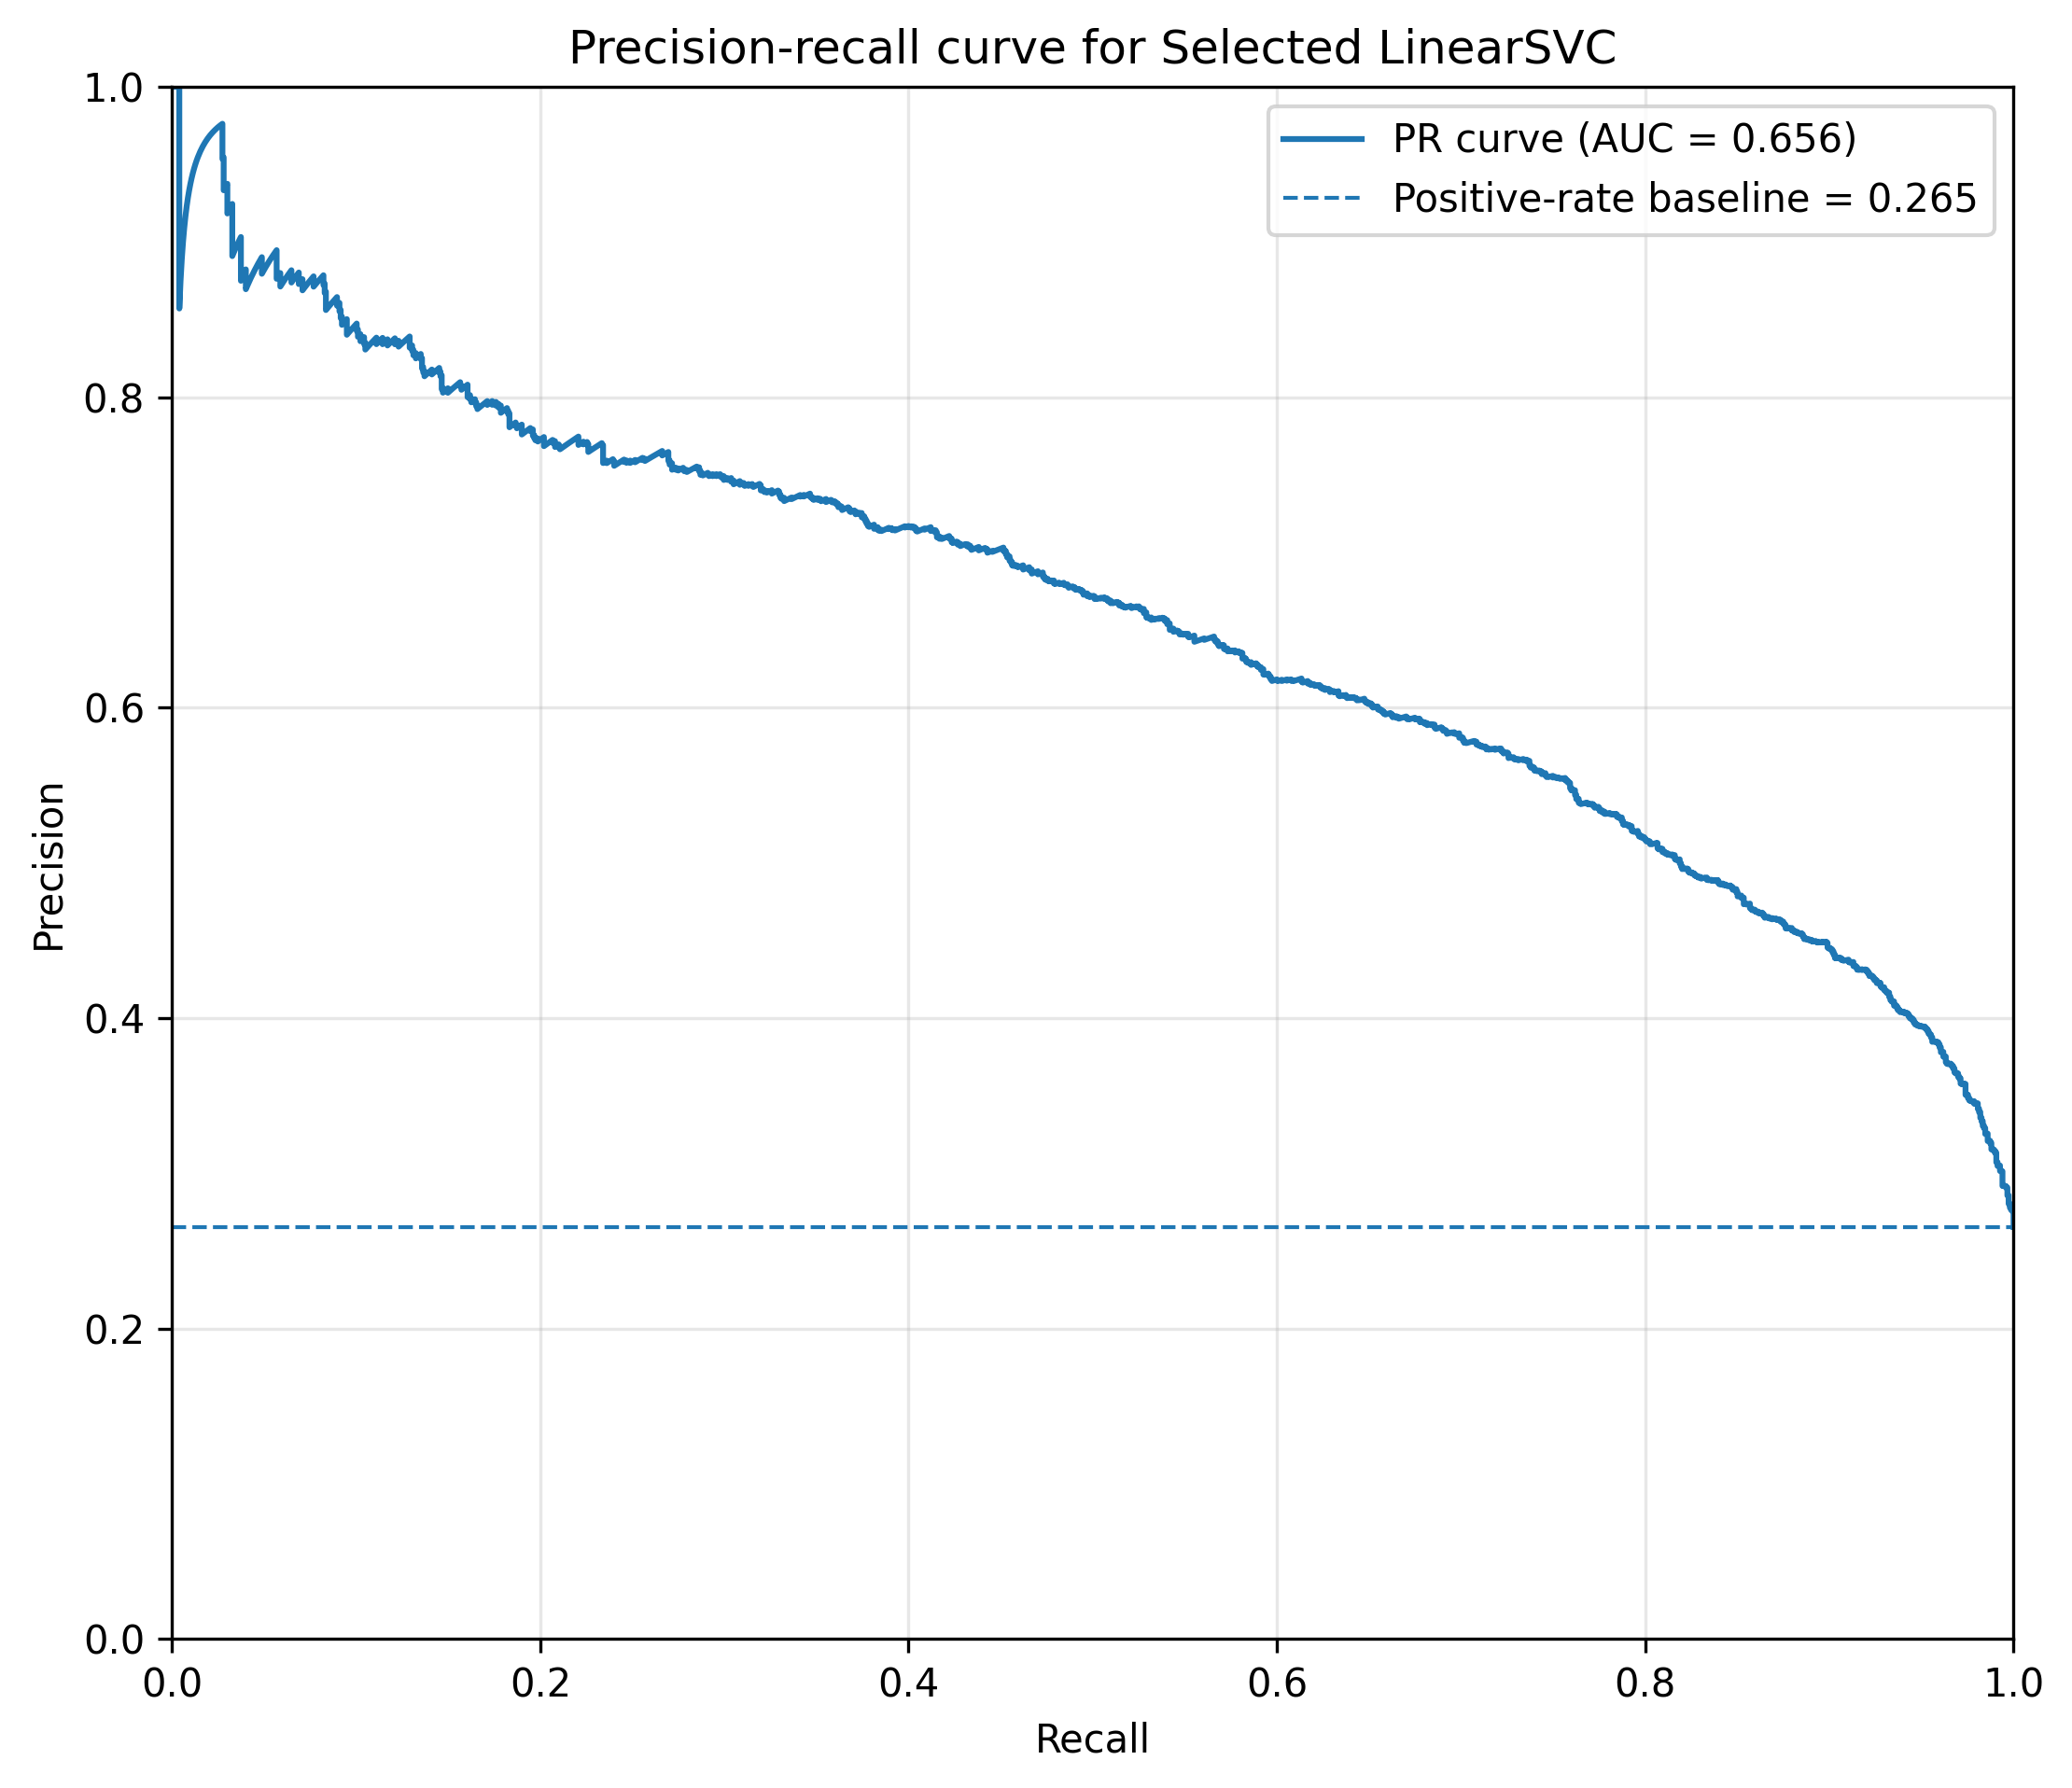
\includegraphics[width=0.82\textwidth]{../figures/svm_precision_recall_curve.png}
\caption{Precision-recall curve for the selected LinearSVC}
\label{fig:svm-pr-curve}
\end{figure}

\subsection{Linear-SVM coefficient directions}

The selected linear SVM is fitted once on the complete training set to inspect coefficient directions. This refit is for interpretation only and does not enter the cross-validated performance estimates. A positive coefficient increases the positive-class SVM decision score, while a negative coefficient decreases it, conditional on the other transformed features.

Table~\ref{tab:svm-linear-coefficients} lists selected large coefficients. The largest positive directions are fiber-optic internet service, month-to-month contract status, streaming services, electronic-check payment, lack of online security, and lack of technical support. The largest negative directions include tenure, DSL service, two-year contract status, and several no-internet-service indicators.

\begin{table}[H]
\centering
\small
\begin{tabular}{lr}
\toprule
Feature & SVM decision-score coefficient \\
\midrule
tenure & -0.322 \\
InternetService\_Fiber optic & 0.279 \\
MonthlyCharges & -0.244 \\
InternetService\_DSL & -0.239 \\
Contract\_Month-to-month & 0.238 \\
Contract\_Two year & -0.223 \\
StreamingMovies\_Yes & 0.107 \\
StreamingTV\_Yes & 0.102 \\
PaymentMethod\_Electronic check & 0.094 \\
OnlineSecurity\_No & 0.083 \\
TechSupport\_No & 0.068 \\
\bottomrule
\end{tabular}
\caption{Selected coefficient directions for the fitted LinearSVC}
\label{tab:svm-linear-coefficients}
\end{table}

\begin{figure}[H]
\centering
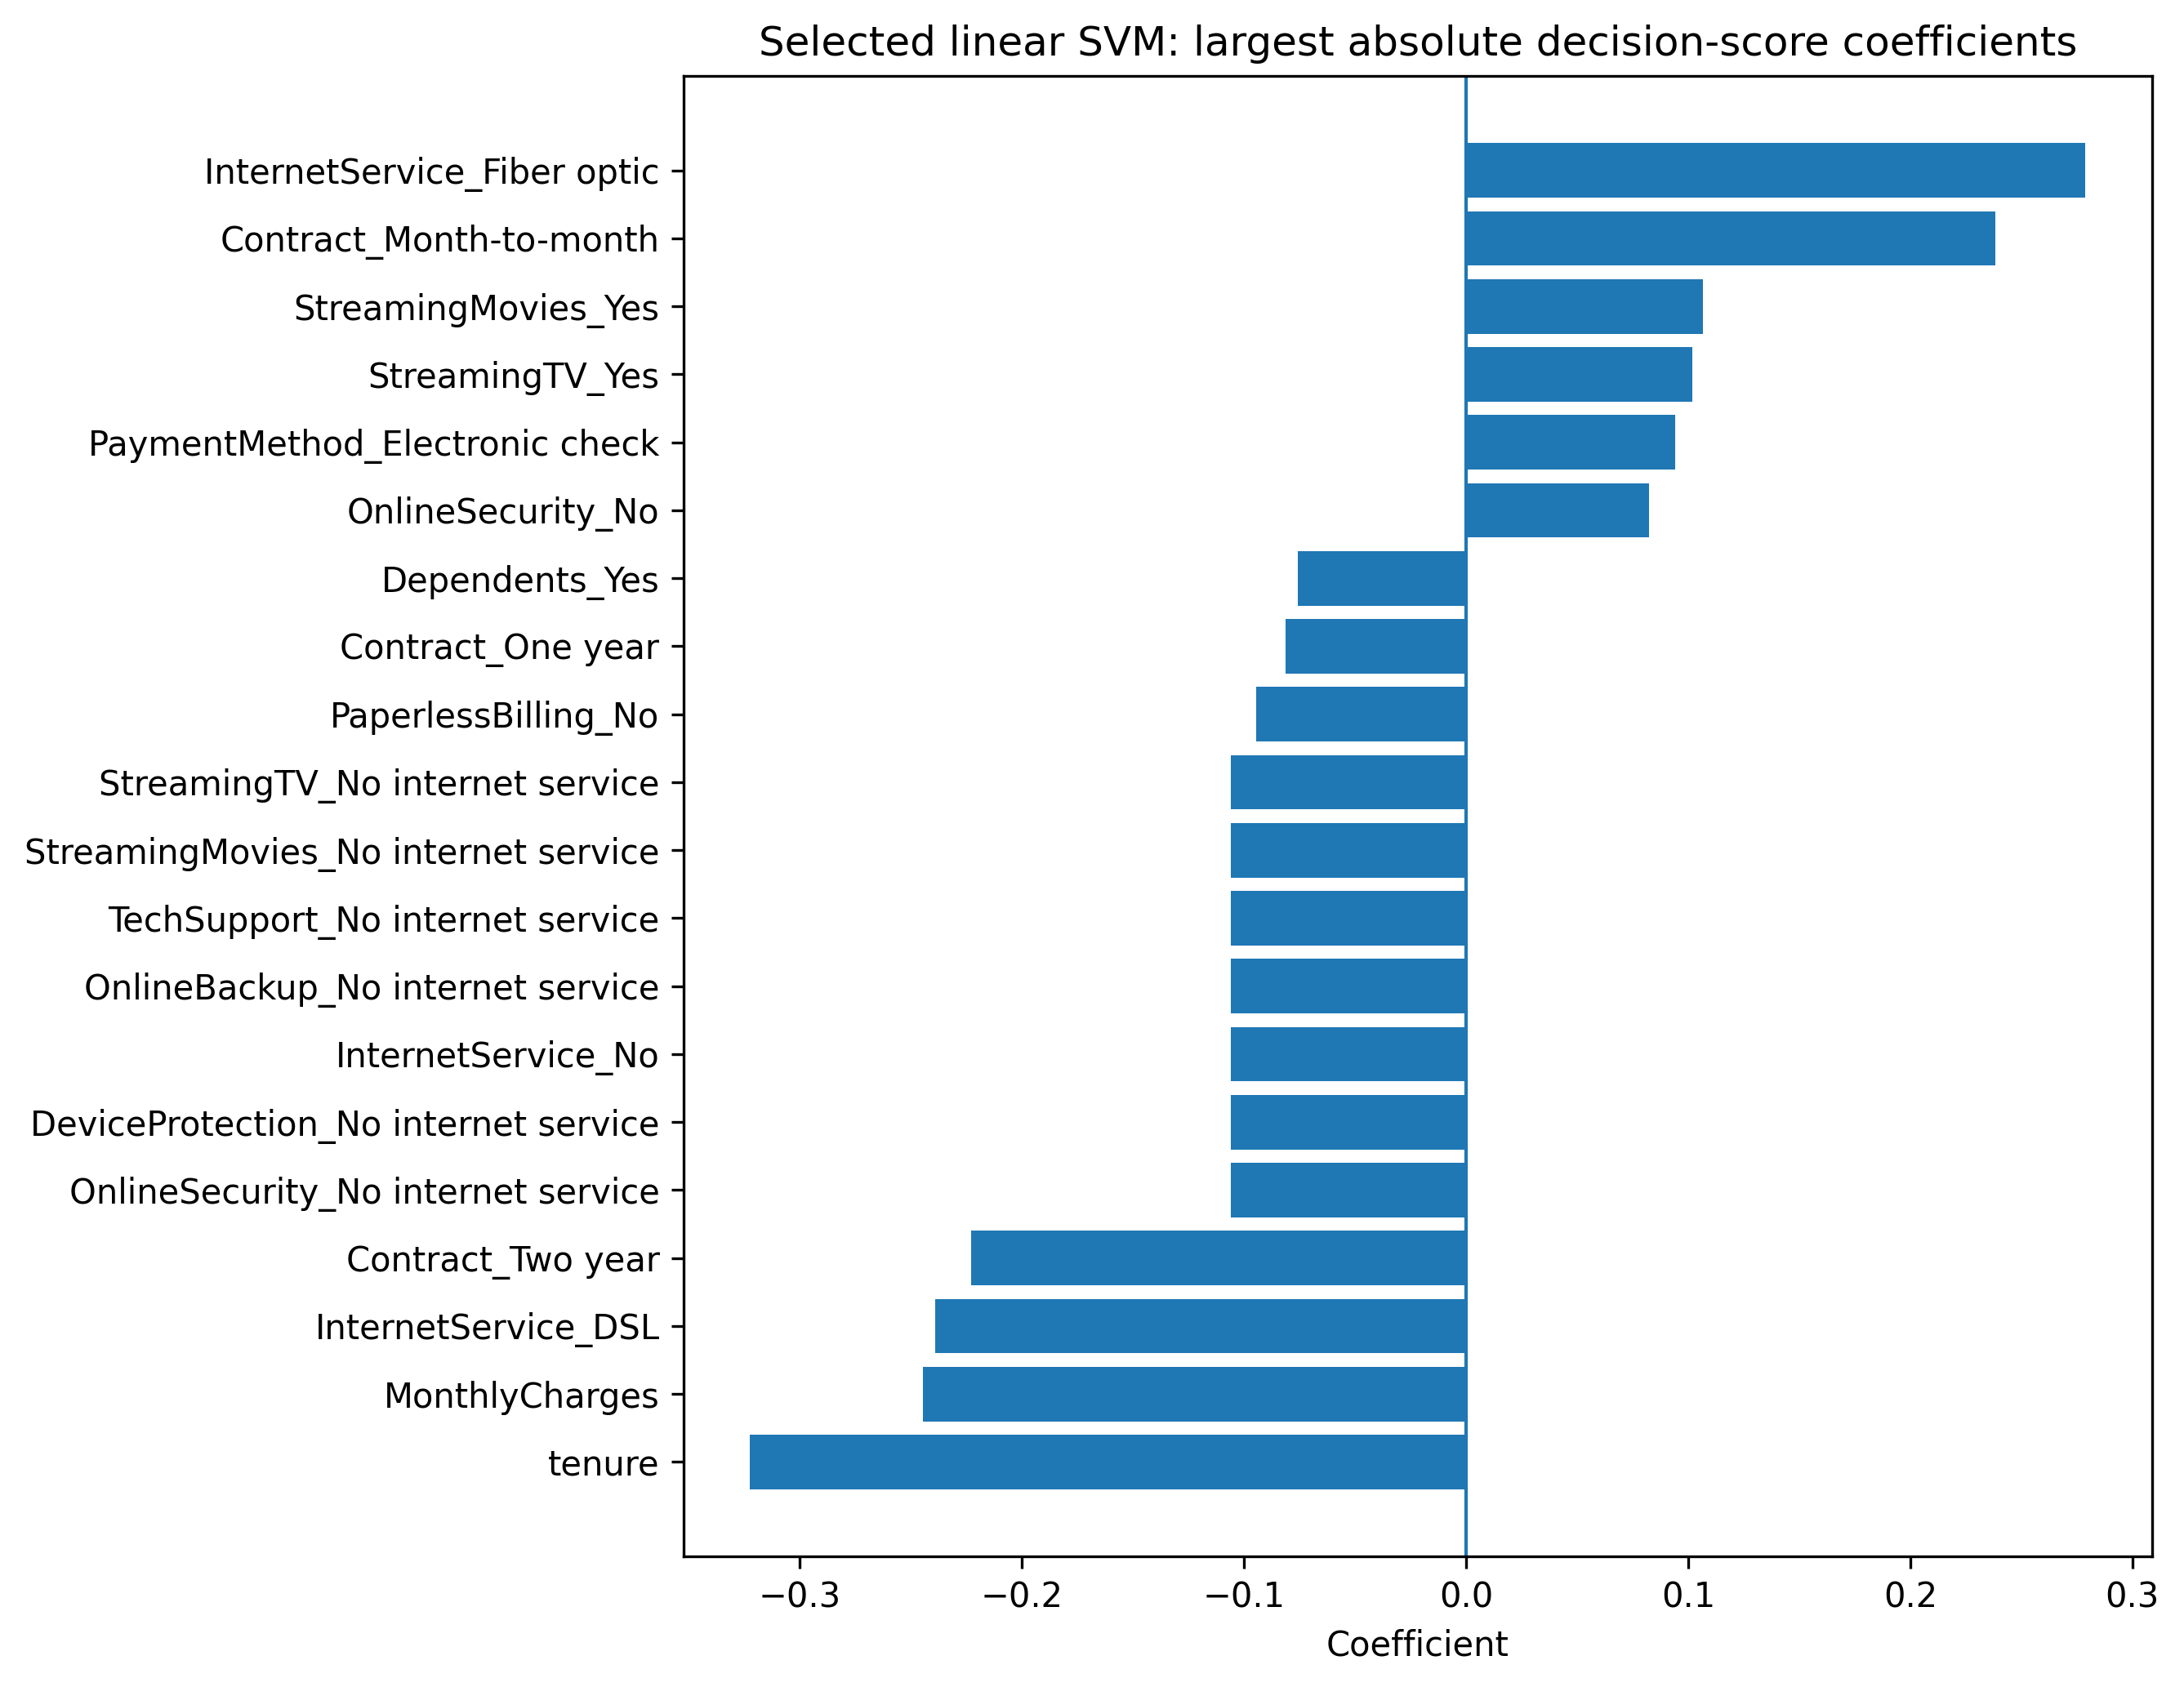
\includegraphics[width=0.84\textwidth]{../figures/svm_linear_coefficients.png}
\caption{Largest absolute decision-score coefficients for the selected LinearSVC}
\label{fig:svm-linear-coefficients}
\end{figure}

The coefficients are not causal effects and are not logistic-regression log-odds coefficients. They must not be exponentiated into odds ratios. They describe how the fitted maximum-margin score changes conditionally within the correlated one-hot encoded representation. In particular, the negative coefficient on \texttt{MonthlyCharges} is conditional on tenure, contract, internet service, and related service features. It should not be interpreted as a marginal statement that higher charges reduce churn.

\subsection{RBF support-vector diagnostic}

The selected RBF SVC is fitted once on the complete training data to summarize its support-vector counts. This is a structural diagnostic only. It does not provide another performance estimate and it does not influence model selection.

\begin{table}[H]
\centering
\small
\begin{tabular}{lrr}
\toprule
Class & Support-vector count & Share of training rows \\
\midrule
Non-churn & 2246 & 0.399 \\
Churn & 816 & 0.145 \\
Total & 3062 & 0.543 \\
\bottomrule
\end{tabular}
\caption{Support-vector diagnostic for the selected RBF SVC fitted on the full training set}
\label{tab:svm-support-vectors}
\end{table}

The selected RBF SVC uses \(3062\) support vectors, equal to approximately \(54.3\%\) of the \(5634\) training observations. A large support-vector share is not inherently problematic, especially in overlapping noisy data. It does show that the nonlinear solution remains structurally more complex than the linear alternative. Because the RBF model does not provide a clear fold-level ranking improvement, this complexity reinforces the preference for the linear SVM as the representative SVM diagnostic model.

\subsection{Section summary}

This section introduced support vector machines as maximum-margin classifiers and evaluated both linear and nonlinear kernel variants. The selected linear configuration uses squared-hinge loss, \(C=0.1\), and balanced class weights. The selected RBF configuration uses \(C=10\), \(\gamma=0.001\), and balanced class weights.

The strongest linear and RBF candidates are effectively tied in mean fold-level validation PR-AUC. The RBF point estimate is only \(0.0001\) higher, far below observed fold-to-fold variation. The kernel-family screen and RBF grid do not demonstrate a material nonlinear advantage, while large \(\gamma\) values show a clear risk of overfitting. The linear SVM is therefore retained as the representative SVM for diagnostics because it is faster, more interpretable, and stronger in the pooled OOF comparison.

The SVM family is competitive with logistic regression and several tree ensembles, but it does not exceed the strongest XGBoost reference in this deliberately scoped comparison. Its class-weighted natural boundary yields high recall at the cost of a substantially larger intervention list. Raw SVM decision scores support ranking and threshold-tradeoff analysis, but they are not calibrated probabilities. A later final training-only comparison will include all serious model-family finalists, define any calibration and threshold procedure, and use the held-out test set exactly once after the complete development policy is fixed.


\newpage
\newpage
\section{Multilayer Perceptrons: Learned Nonlinear Representations}
\label{sec:multilayer-perceptrons}

This section evaluates a feed-forward multilayer perceptron (MLP) for churn prediction. An MLP extends a linear classifier by learning intermediate nonlinear feature transformations before it constructs the final churn score. This makes the model capable of representing interactions and nonlinear decision surfaces that would not be available to an ordinary additive logistic-regression specification without manually engineered interaction or basis features.

The held-out test set is not used anywhere in this section. Candidate architectures, regularization strengths, activation diagnostics, threshold curves, calibration diagnostics, and comparisons are produced from the training set only through the project's stratified cross-validation design. The reported configuration is therefore a development-stage candidate, not a final globally optimized neural network and not a final estimate of test performance. This maintains the train--validation--test separation used throughout the project \cite{ml-evaluation,dl-tools}.

\subsection{From logistic regression to learned nonlinear features}

For a transformed feature vector \(x\in\mathbb{R}^{d}\), logistic regression constructs one affine score
\[
\eta(x)=w^\top x+b
\]
and converts it into a churn probability through the sigmoid function
\[
\widehat{p}(x)=\sigma(\eta(x))
=
\frac{1}{1+\exp\{-\eta(x)\}}.
\]
The resulting boundary is linear in the transformed input space. One-hot encoded indicators permit different categorical groups to have different additive effects, but the model cannot automatically create arbitrary interactions such as a particular combination of contract type, internet service, tenure, and monthly charge.

An MLP instead learns hidden representations. For a network with \(L\) hidden layers, let \(h^{(0)}=x\). Each hidden layer applies an affine transformation followed by an element-wise nonlinearity:
\[
z^{(\ell)}
=
W^{(\ell)}h^{(\ell-1)}+b^{(\ell)},
\qquad
h^{(\ell)}
=
\phi\!\left(z^{(\ell)}\right),
\qquad
\ell=1,\ldots,L.
\]
The binary output layer produces a logit
\[
\eta(x)
=
w_{\mathrm{out}}^\top h^{(L)}+b_{\mathrm{out}},
\]
followed by
\[
\widehat{p}(x)
=
\sigma\!\left(\eta(x)\right).
\]

The activation function is essential. If every layer were affine, then the composition of layers would remain affine:
\[
W^{(2)}(W^{(1)}x+b^{(1)})+b^{(2)}
=
\underbrace{W^{(2)}W^{(1)}}_{\widetilde{W}}x
+
\underbrace{W^{(2)}b^{(1)}+b^{(2)}}_{\widetilde{b}}.
\]
Thus, stacking linear layers without nonlinear activation would not increase the functional class beyond a single linear model. The nonlinear transformation \(\phi\) permits the network to learn nonlinear representations.

\subsection{Hidden units, ReLU activations, and network capacity}

The principal candidates use the rectified linear unit,
\[
\operatorname{ReLU}(a)
=
\max\{0,a\}.
\]
ReLU creates a piecewise-linear nonlinear representation. It is computationally simple and avoids the severe saturation that can occur with sigmoid activations in hidden layers. A small \(\tanh\) diagnostic is also evaluated:
\[
\tanh(a)
=
\frac{\exp(a)-\exp(-a)}{\exp(a)+\exp(-a)}.
\]
Unlike ReLU, \(\tanh\) is bounded between \(-1\) and \(1\), which can be useful in some settings but may create smaller gradients when units saturate.

The selected architecture has one hidden layer with \(16\) ReLU units. The dense preprocessing pipeline produces \(46\) numeric input columns after fold-internal median imputation, standardization of numeric variables, and dense one-hot encoding of categorical variables. The number of trainable parameters is therefore
\[
(46+1)\times16+(16+1)\times1=769.
\]
The first term represents the hidden-layer weights and biases; the second represents the output-layer weights and bias. This is intentionally a modest capacity relative to the \(5{,}634\) training observations. Wider or deeper networks have more representational flexibility, but also more variance, more optimization sensitivity, and more opportunity to fit fold-specific idiosyncrasies.

\subsection{Binary cross-entropy and backpropagation}

The network is trained through the Bernoulli negative log-likelihood, commonly called binary cross-entropy:
\[
\mathcal{L}_{\mathrm{BCE}}
=
-\frac{1}{n}
\sum_{i=1}^{n}
\left[
y_i\log\widehat{p}_i
+
(1-y_i)\log(1-\widehat{p}_i)
\right].
\]
For a sigmoid output and binary cross-entropy, the derivative of the loss with respect to the output logit takes the particularly simple form
\[
\frac{\partial \mathcal{L}_{\mathrm{BCE}}}{\partial \eta_i}
=
\widehat{p}_i-y_i.
\]
Backpropagation applies the chain rule from this output error through the network. Writing \(\delta^{(L+1)}=\widehat{p}-y\) for the output error, the hidden-layer errors are propagated recursively:
\[
\delta^{(\ell)}
=
\left(W^{(\ell+1)\top}\delta^{(\ell+1)}\right)
\odot
\phi'\!\left(z^{(\ell)}\right).
\]
For a mini-batch of size \(m\), the gradient for a weight matrix is proportional to
\[
\nabla_{W^{(\ell)}}\mathcal{L}
=
\frac{1}{m}\delta^{(\ell)}h^{(\ell-1)\top}.
\]
The optimizer then updates every weight and bias in the direction that lowers the loss.

The implementation uses the Adam optimizer. Adam maintains running estimates of the first and second moments of the gradients and rescales updates coordinate by coordinate. This is convenient for a tabular model with a mixture of standardized continuous inputs and sparse one-hot indicators, but it does not remove the need for validation-based regularization and careful comparison.

\subsection{Regularization, early stopping, and leakage-safe preprocessing}

The MLP uses an L2 penalty, controlled by scikit-learn's \texttt{alpha} parameter:
\[
\mathcal{L}_{\mathrm{regularized}}
=
\mathcal{L}_{\mathrm{BCE}}
+
\frac{\alpha}{2n}\sum_{\ell}\left\lVert W^{(\ell)}\right\rVert_F^2.
\]
A larger \(\alpha\) shrinks weights more strongly and can reduce variance, while an overly large value may suppress useful structure.

Every MLP candidate is an sklearn pipeline. Numeric imputers, standardization parameters, category levels, and one-hot mappings are fitted only on each outer cross-validation training fold. This is necessary because neural networks are sensitive to numeric scale and because fitting preprocessing once on the complete training set would leak validation-fold distributional information into each fold's model.

The \texttt{MLPClassifier} candidates also use internal early stopping. Within an outer training fold, the classifier reserves \(15\%\) of that fold for its own internal validation split and stops after \(20\) iterations without an improvement in its internal validation accuracy. The outer-fold PR-AUC remains the model-selection metric. Internal validation accuracy is a training-control diagnostic, not the primary business or model-family selection criterion.

\subsection{Training-only search design}

The workflow uses a deliberately compact staged search rather than an exhaustive neural-network sweep. The initial shallow ReLU grid evaluates widths \(16\), \(32\), and \(64\), crossed with L2 strengths
\[
\alpha\in\{0.0001,0.001,0.01\}.
\]
The widths are geometrically spaced and the L2 values are logarithmically spaced. This is appropriate because a doubling of width or a tenfold change in a regularization scale is typically more meaningful than an arbitrary small additive change.

After the shallow grid, two two-hidden-layer architectures are evaluated using the strongest observed shallow-grid L2 value. Finally, the strongest ReLU architecture is compared with a \(\tanh\) version of the same architecture. This is a training-only development procedure, but it is not a fully predeclared Cartesian grid across every architecture, activation, and regularization combination. Consequently, small differences must not be interpreted as evidence of a uniquely optimal MLP.

\subsection{Shallow ReLU screen}

Table~\ref{tab:mlp-shallow-grid} reports the nine shallow ReLU candidates. The largest mean fold-level validation PR-AUC is \(0.6595\), achieved by the \(16\)-unit network with \(\alpha=0.001\). The \(16\)-unit alternatives are essentially tied: the difference between the selected configuration and the next candidate is only \(0.0007\), while their fold-level PR-AUC standard deviations are around \(0.018\)--\(0.019\).

The wider networks do not improve the main ranking metric. They also display larger train--validation PR-AUC gaps, especially for \(64\) hidden units. This pattern does not prove overfitting in a formal population sense, but it is consistent with extra capacity fitting the outer-fold training partitions more strongly without producing better validation ranking.

\begin{table}[H]
\centering
\small
\resizebox{\textwidth}{!}{
\begin{tabular}{lrrrrrrr}
\toprule
Hidden units & \(\alpha\) & Mean CV PR-AUC & SD & Mean CV ROC-AUC & Bal. Acc. & \(F_1\) & Train--valid. PR gap \\
\midrule
\(16\) & 0.0010 & 0.6595 & 0.0183 & 0.8436 & 0.7108 & 0.5798 & 0.0096 \\
\(16\) & 0.0100 & 0.6588 & 0.0189 & 0.8432 & 0.7126 & 0.5828 & 0.0099 \\
\(16\) & 0.0001 & 0.6586 & 0.0193 & 0.8428 & 0.7077 & 0.5748 & 0.0079 \\
\(32\) & 0.0100 & 0.6580 & 0.0215 & 0.8442 & 0.7206 & 0.5964 & 0.0215 \\
\(32\) & 0.0010 & 0.6576 & 0.0213 & 0.8440 & 0.7164 & 0.5890 & 0.0158 \\
\(32\) & 0.0001 & 0.6567 & 0.0208 & 0.8441 & 0.7152 & 0.5869 & 0.0172 \\
\(64\) & 0.0010 & 0.6567 & 0.0156 & 0.8423 & 0.7153 & 0.5876 & 0.0385 \\
\(64\) & 0.0100 & 0.6565 & 0.0158 & 0.8426 & 0.7204 & 0.5942 & 0.0302 \\
\(64\) & 0.0001 & 0.6559 & 0.0156 & 0.8425 & 0.7170 & 0.5902 & 0.0383 \\
\bottomrule
\end{tabular}
}
\caption{Shallow ReLU MLP screen using mean outer-fold validation metrics. The train--validation gap is mean train PR-AUC minus mean validation PR-AUC.}
\label{tab:mlp-shallow-grid}
\end{table}

\begin{figure}[H]
\centering
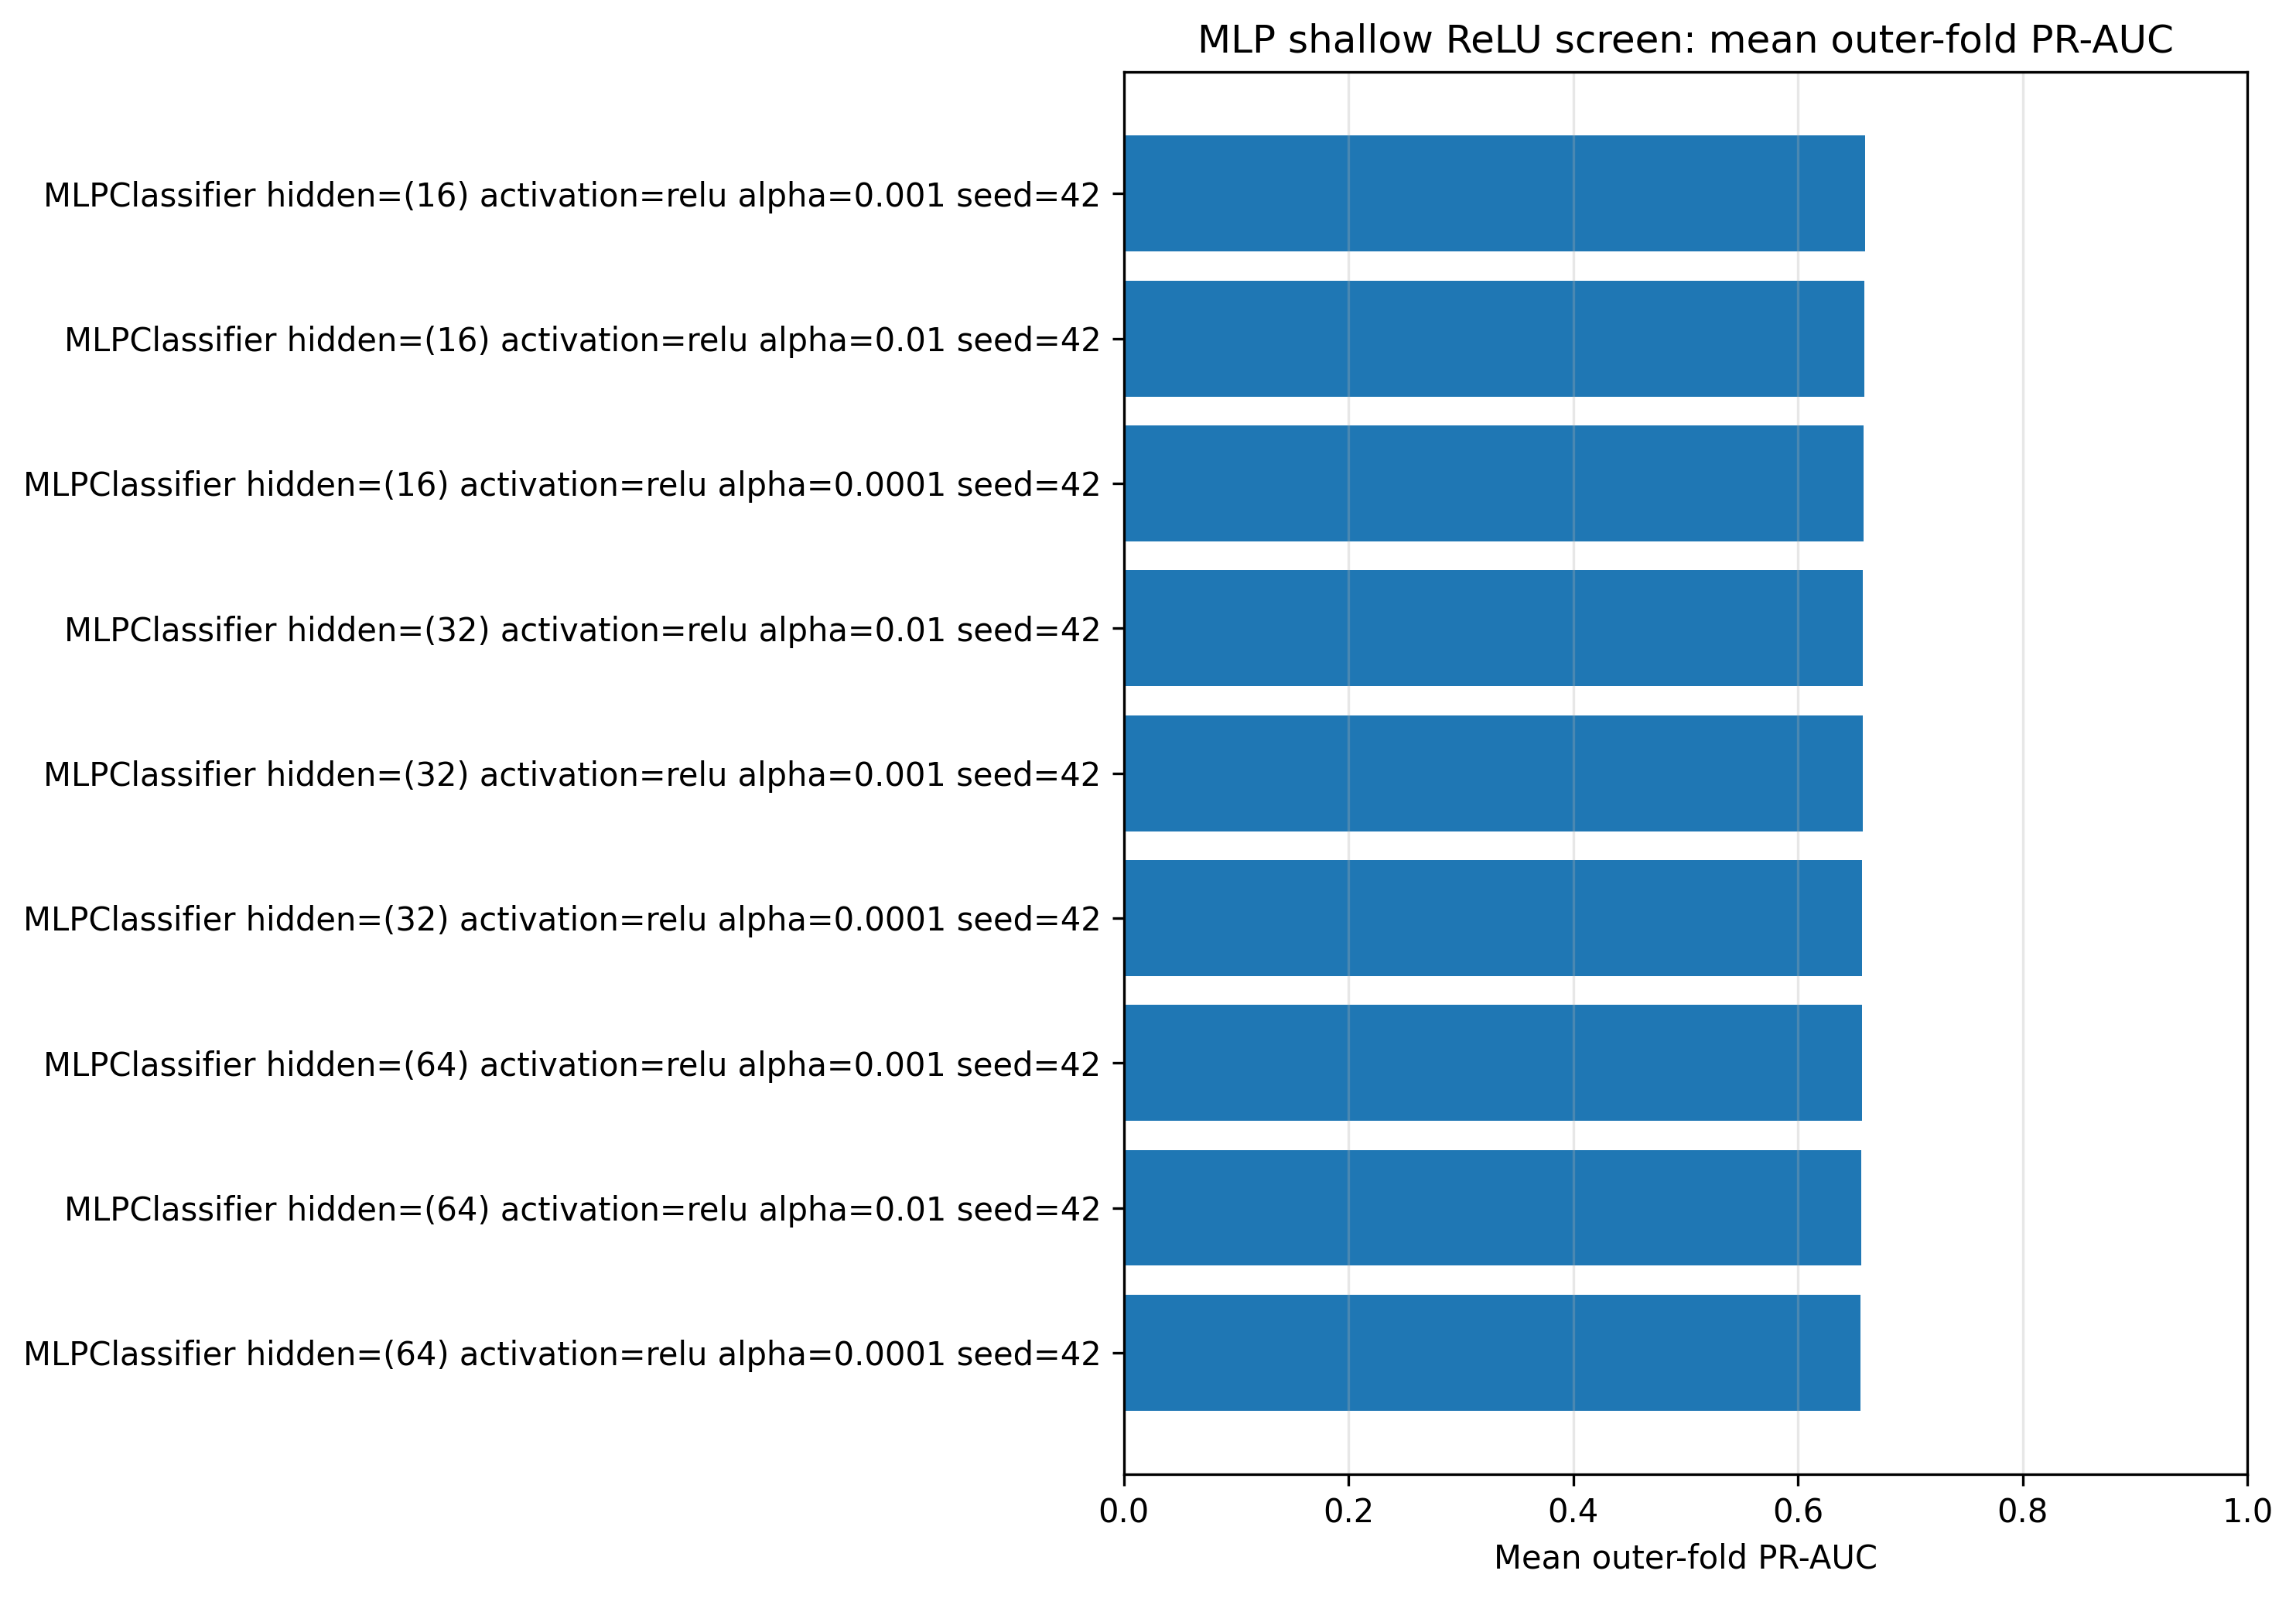
\includegraphics[width=0.90\textwidth]{../figures/mlp_shallow_grid_pr_auc.png}
\caption{Shallow ReLU MLP candidates ranked by mean outer-fold PR-AUC}
\label{fig:mlp-shallow-grid}
\end{figure}

\subsection{Depth and activation diagnostics}

Adding a second hidden layer does not improve the observed ranking quality. The \((64,32)\) architecture reaches mean CV PR-AUC \(0.6523\), while \((32,16)\) reaches \(0.6507\), both below the selected one-hidden-layer candidate. The \(\tanh\) version of the selected \(16\)-unit architecture reaches \(0.6559\), also below the ReLU result.

These diagnostics suggest that the available feature representation and sample size do not provide a visible benefit from additional depth or the alternative hidden activation. They do not imply that deep networks are universally unsuitable for tabular data. They only describe this compact candidate set on this dataset.

\begin{table}[H]
\centering
\small
\begin{tabular}{llrrrrr}
\toprule
Architecture & Activation & Mean CV PR-AUC & SD & Mean CV ROC-AUC & \(F_1\) & Train--valid. PR gap \\
\midrule
\(16\) & ReLU & 0.6595 & 0.0183 & 0.8436 & 0.5798 & 0.0096 \\
\((64,32)\) & ReLU & 0.6523 & 0.0196 & 0.8407 & 0.5891 & 0.0220 \\
\((32,16)\) & ReLU & 0.6507 & 0.0196 & 0.8444 & 0.5819 & 0.0275 \\
\(16\) & \(\tanh\) & 0.6559 & 0.0273 & 0.8409 & 0.5766 & 0.0062 \\
\bottomrule
\end{tabular}
\caption{Depth and activation diagnostics after the shallow ReLU screen}
\label{tab:mlp-depth-activation}
\end{table}

\begin{figure}[H]
\centering
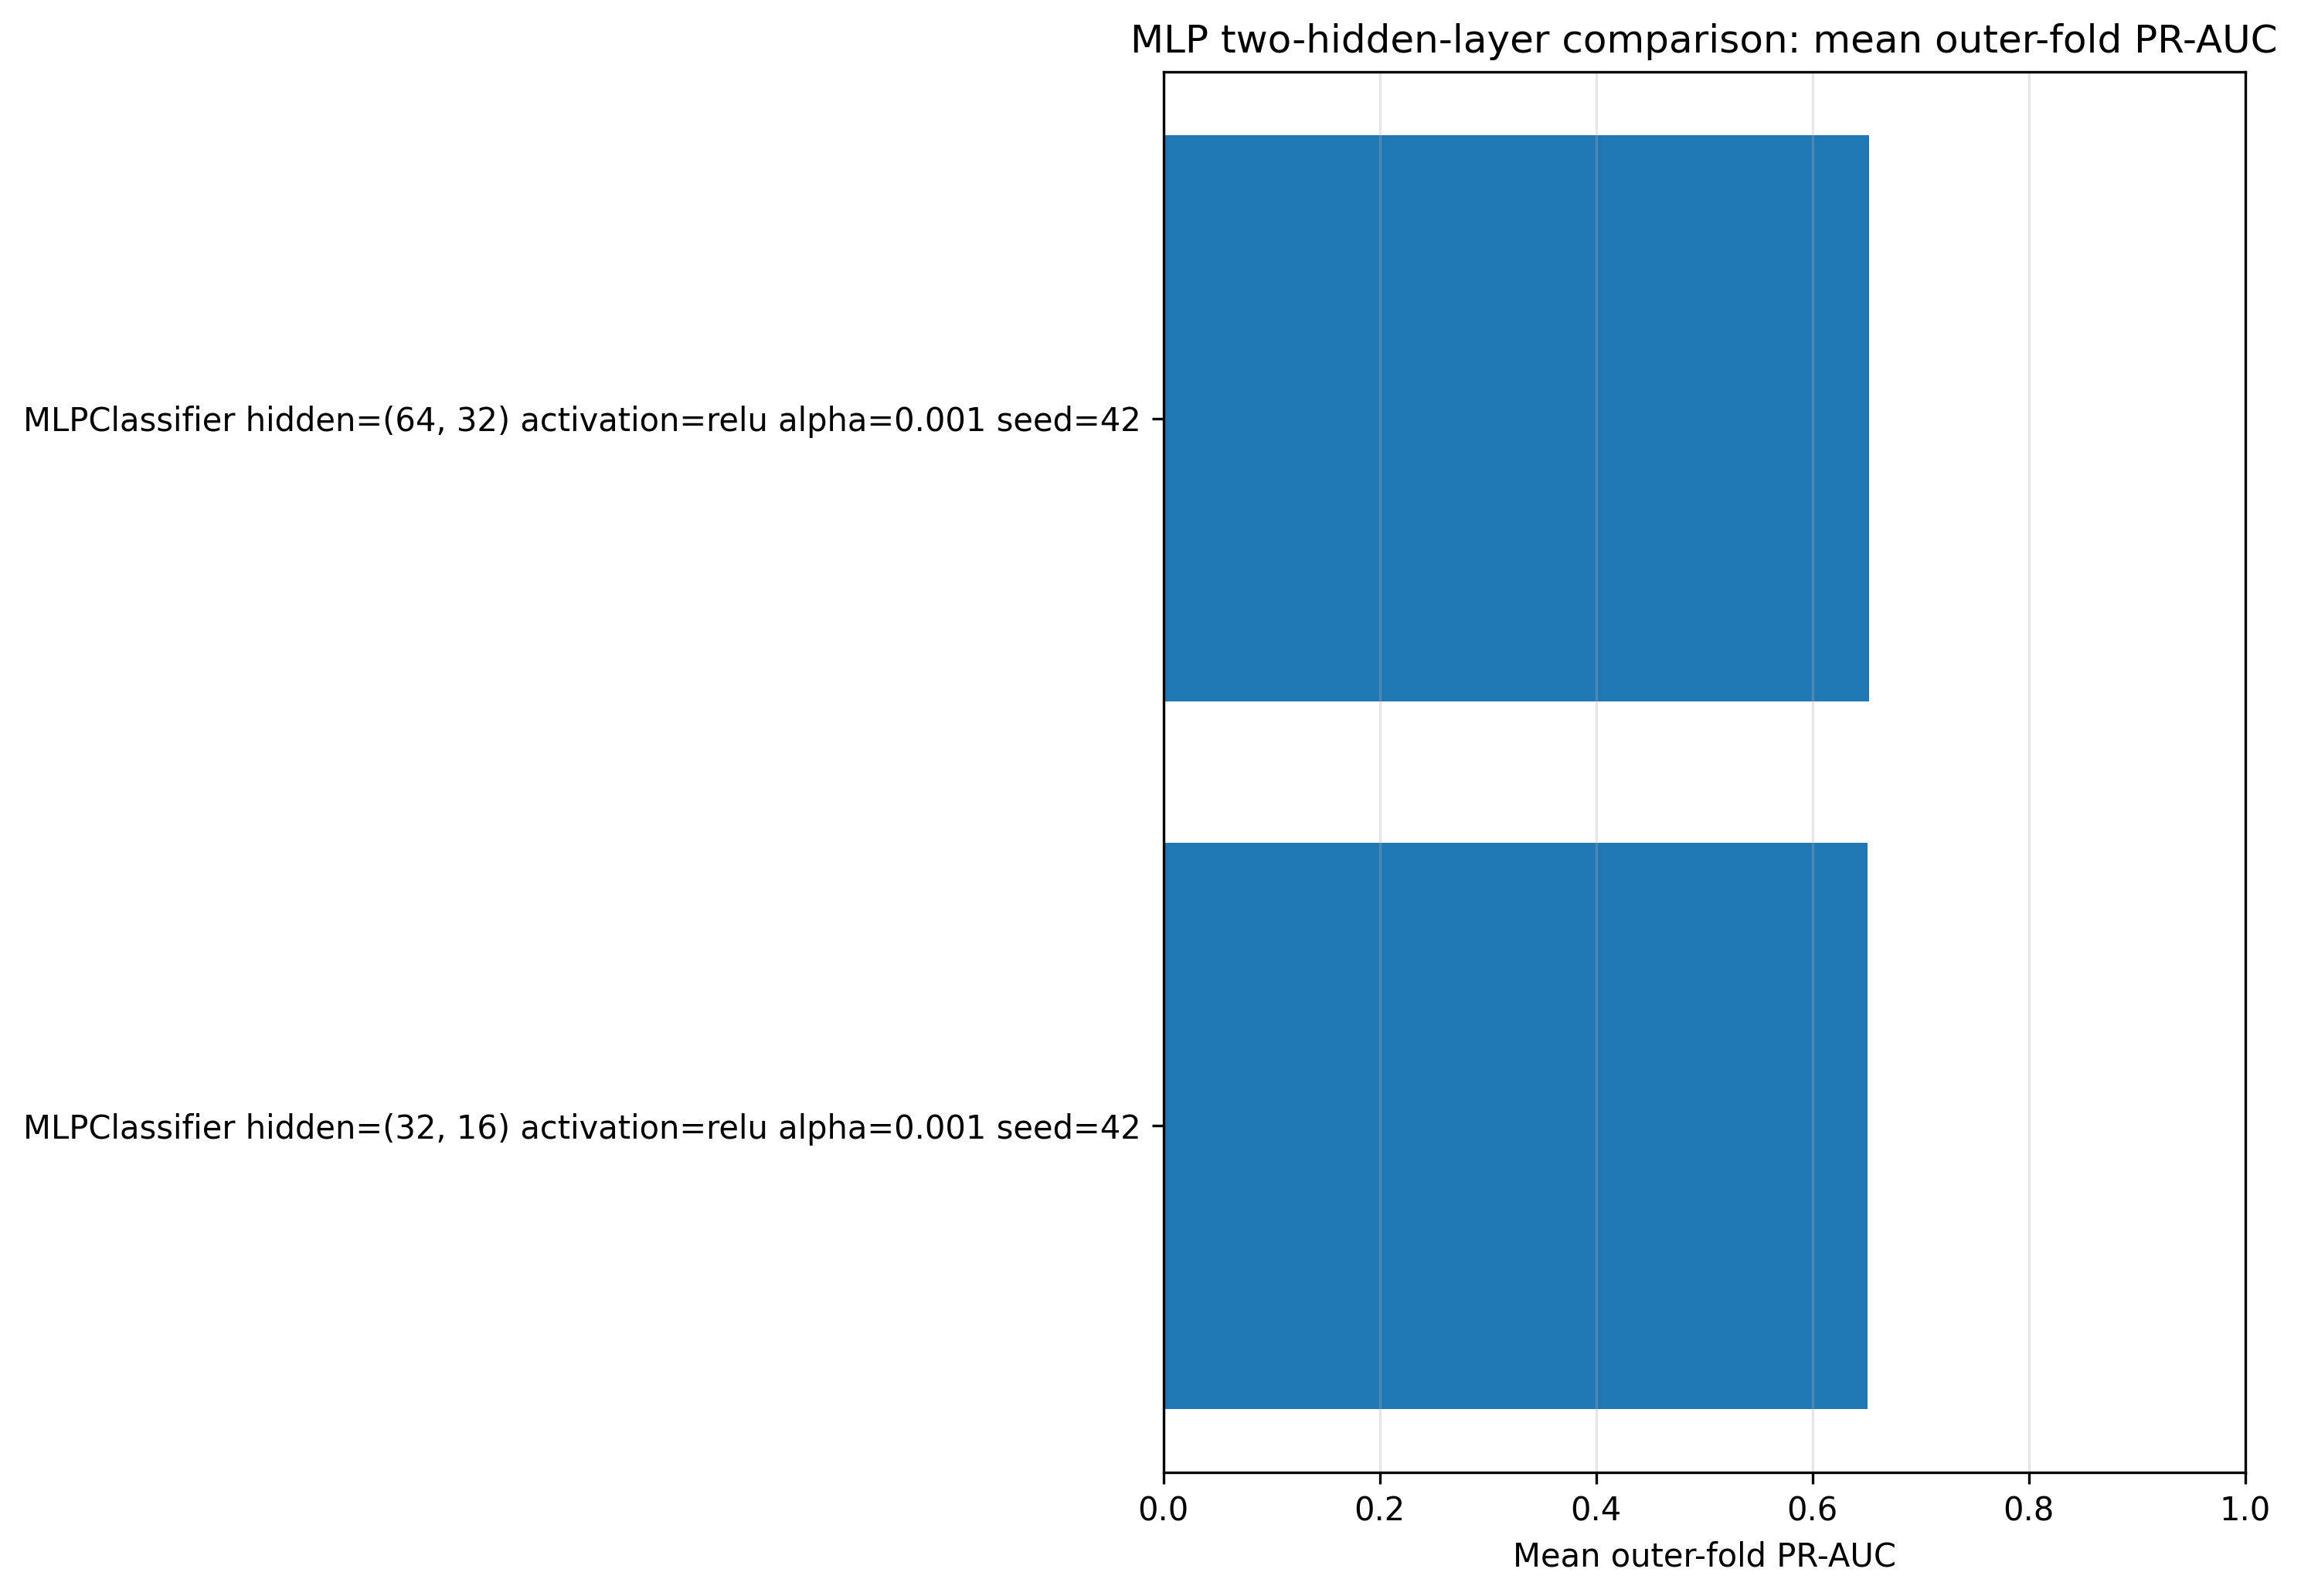
\includegraphics[width=0.84\textwidth]{../figures/mlp_depth_comparison_pr_auc.png}
\caption{Two-hidden-layer MLP diagnostic: mean outer-fold PR-AUC}
\label{fig:mlp-depth-comparison}
\end{figure}

\subsection{Selected MLP and pooled out-of-fold evaluation}

The development-stage representative is the one-hidden-layer ReLU network with \(16\) units and \(\alpha=0.001\). It was selected by mean outer-fold PR-AUC, followed by balanced accuracy and \(F_1\). Its grid-selection statistic is mean fold-level PR-AUC \(0.6595\). When one out-of-fold probability is concatenated for each training observation, the pooled OOF PR-AUC is \(0.6544\) and the pooled OOF ROC-AUC is \(0.8425\).

Mean fold-level PR-AUC and pooled OOF PR-AUC are different statistics. Average precision is nonlinear, and each fold is fitted independently. The mean fold-level score remains the pre-specified grid-selection statistic. The pooled OOF probabilities are used for common diagnostics such as the ROC curve, PR curve, calibration diagnostic, confusion matrix, and threshold analysis.

At the default probability threshold \(0.50\), the MLP identifies \(769\) of \(1495\) churners and produces \(384\) false positives. Its precision is \(0.667\), recall is \(0.514\), and specificity is \(0.907\). The model flags \(20.5\%\) of customers as likely churners, below the observed churn rate of \(26.5\%\). Thus, the unweighted default operating point is relatively conservative: it produces a selective list with good precision and specificity, but it misses nearly half of the observed churners.

\begin{table}[H]
\centering
\small
\begin{tabular}{lrrrrrrrr}
\toprule
Model & Accuracy & Bal. Acc. & Precision & Recall & Specificity & \(F_1\) & ROC-AUC & PR-AUC \\
\midrule
Selected MLP & 0.803 & 0.711 & 0.667 & 0.514 & 0.907 & 0.581 & 0.842 & 0.654 \\
\bottomrule
\end{tabular}
\caption{Pooled out-of-fold diagnostics for the selected MLP}
\label{tab:mlp-selected-oof}
\end{table}

\begin{table}[H]
\centering
\small
\begin{tabular}{rrrrr}
\toprule
TP & FN & FP & TN & Predicted positive rate \\
\midrule
769 & 726 & 384 & 3755 & 0.205 \\
\bottomrule
\end{tabular}
\caption{Positive-first pooled out-of-fold confusion-matrix counts for the selected MLP at threshold \(0.50\)}
\label{tab:mlp-confusion}
\end{table}

\begin{figure}[H]
\centering
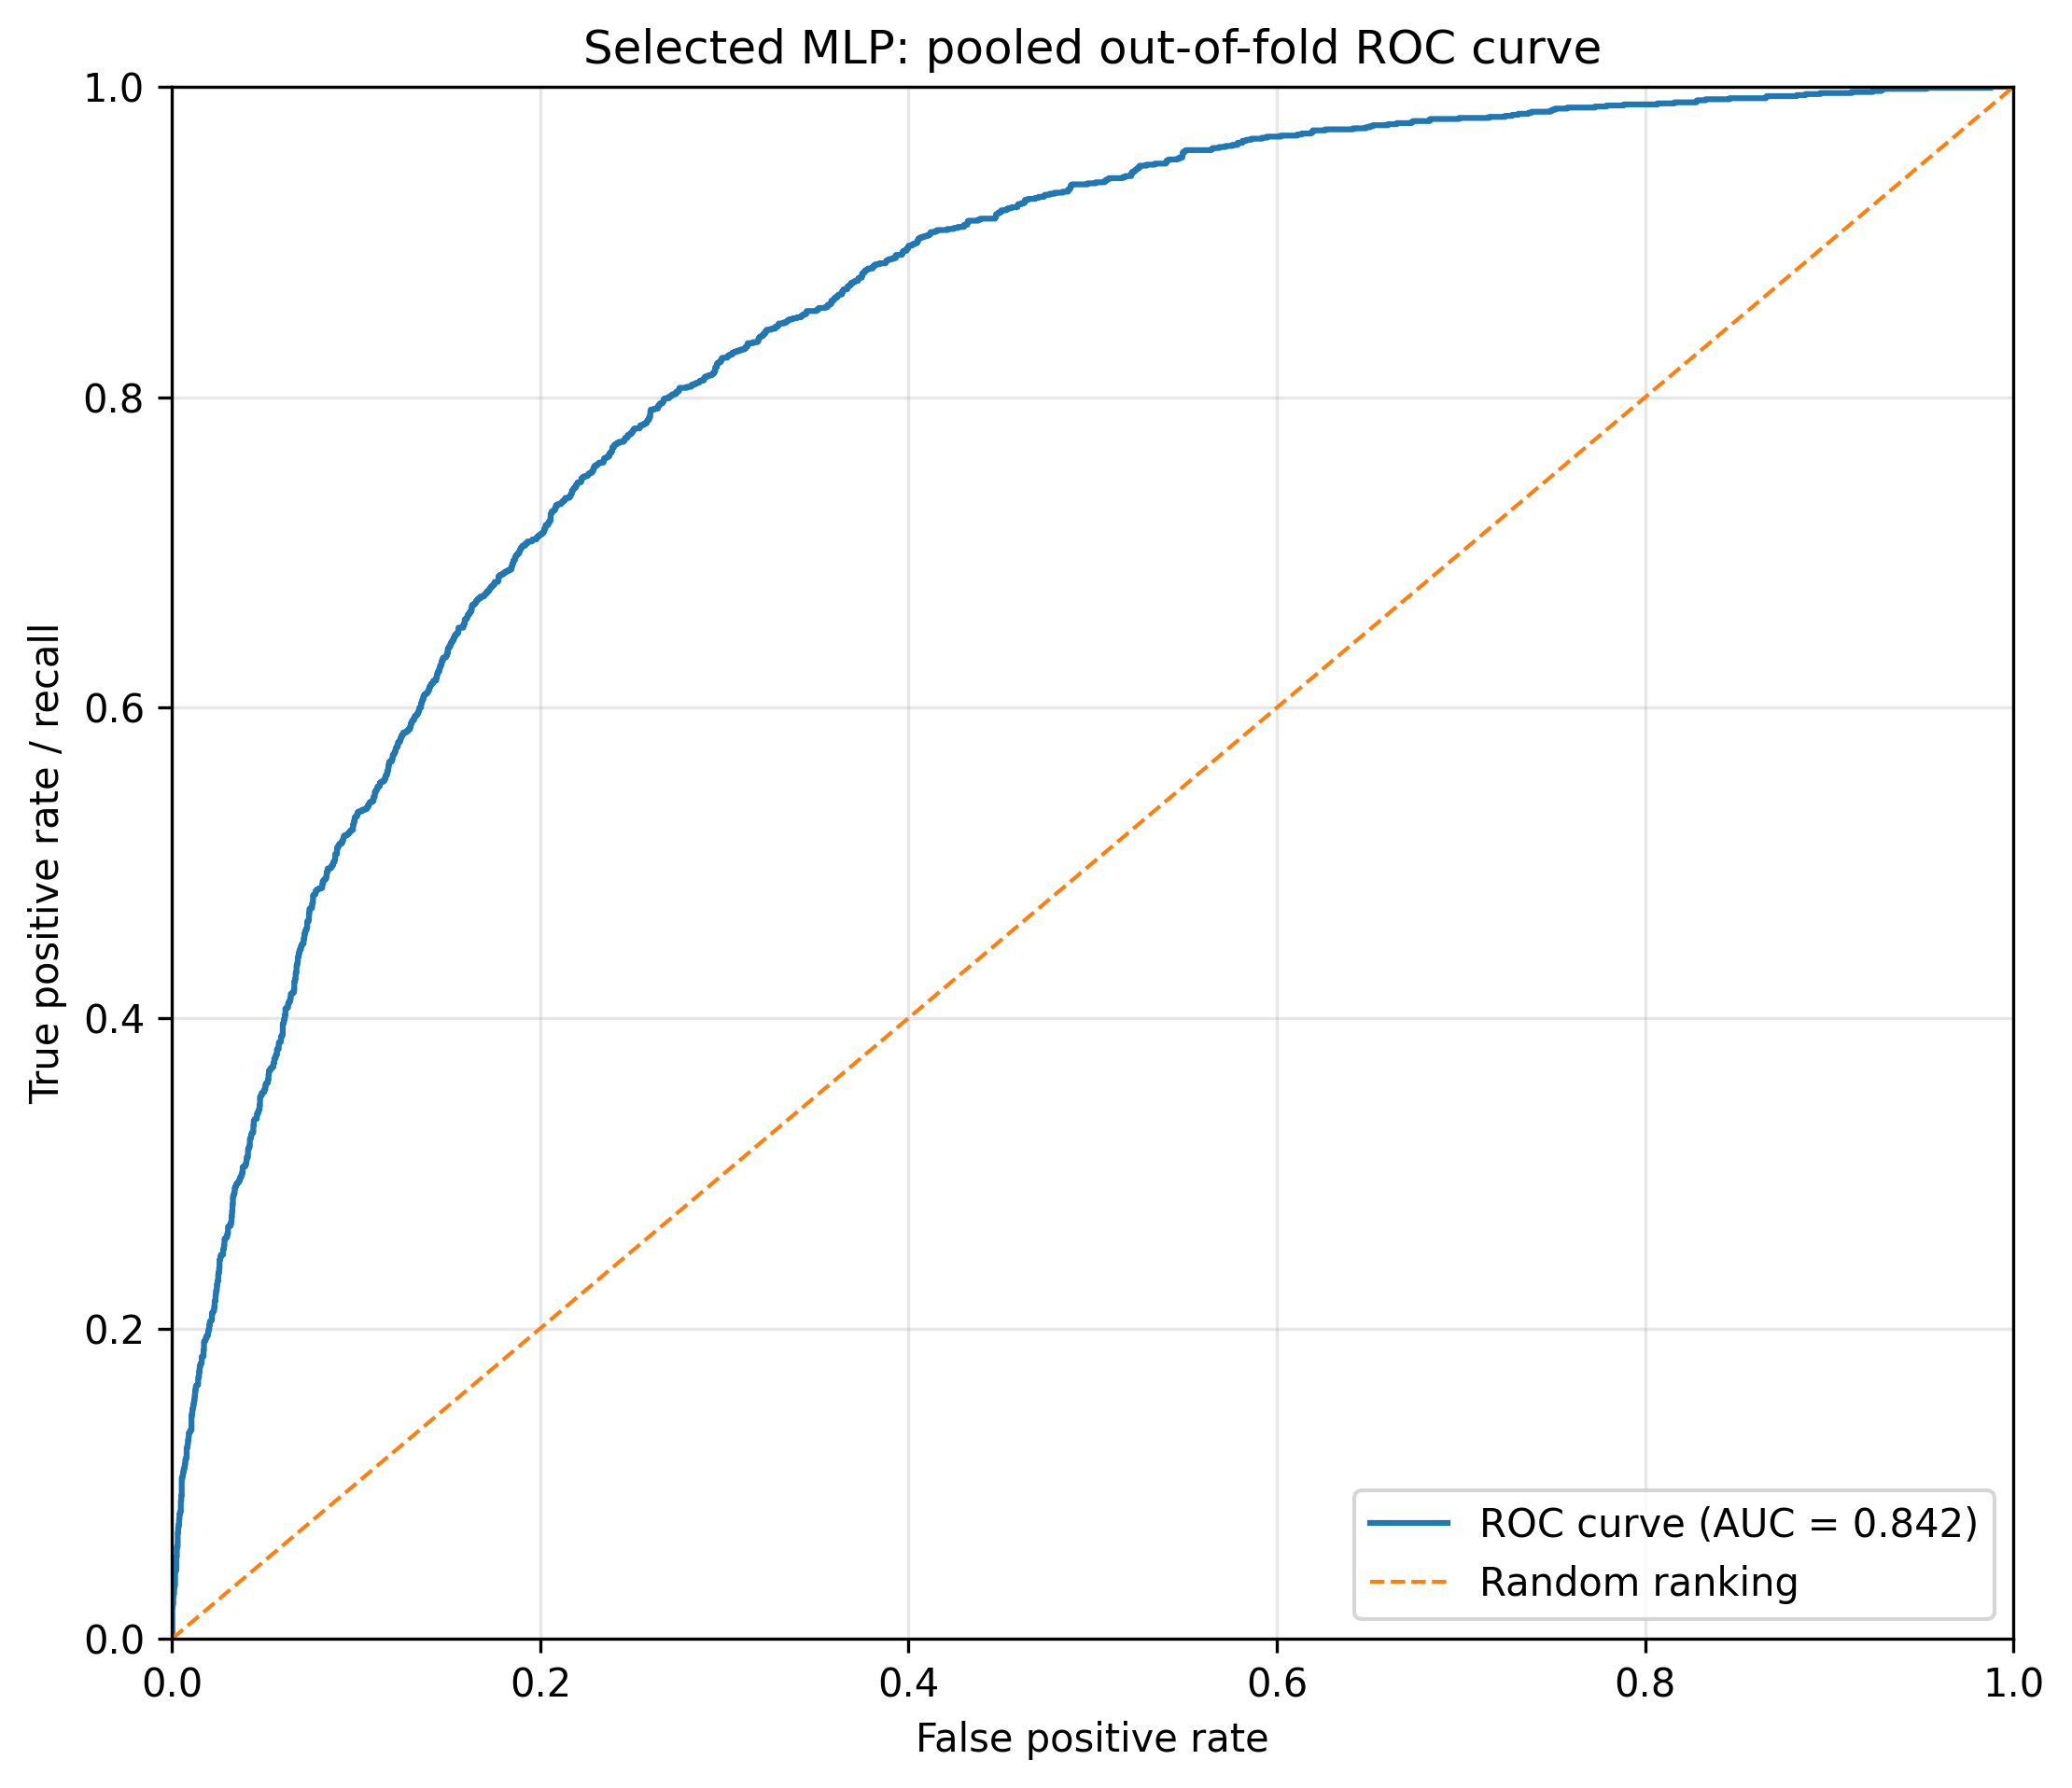
\includegraphics[width=0.82\textwidth]{../figures/mlp_roc_curve.png}
\caption{ROC curve for the selected MLP using pooled out-of-fold churn probabilities}
\label{fig:mlp-roc-curve}
\end{figure}

\begin{figure}[H]
\centering
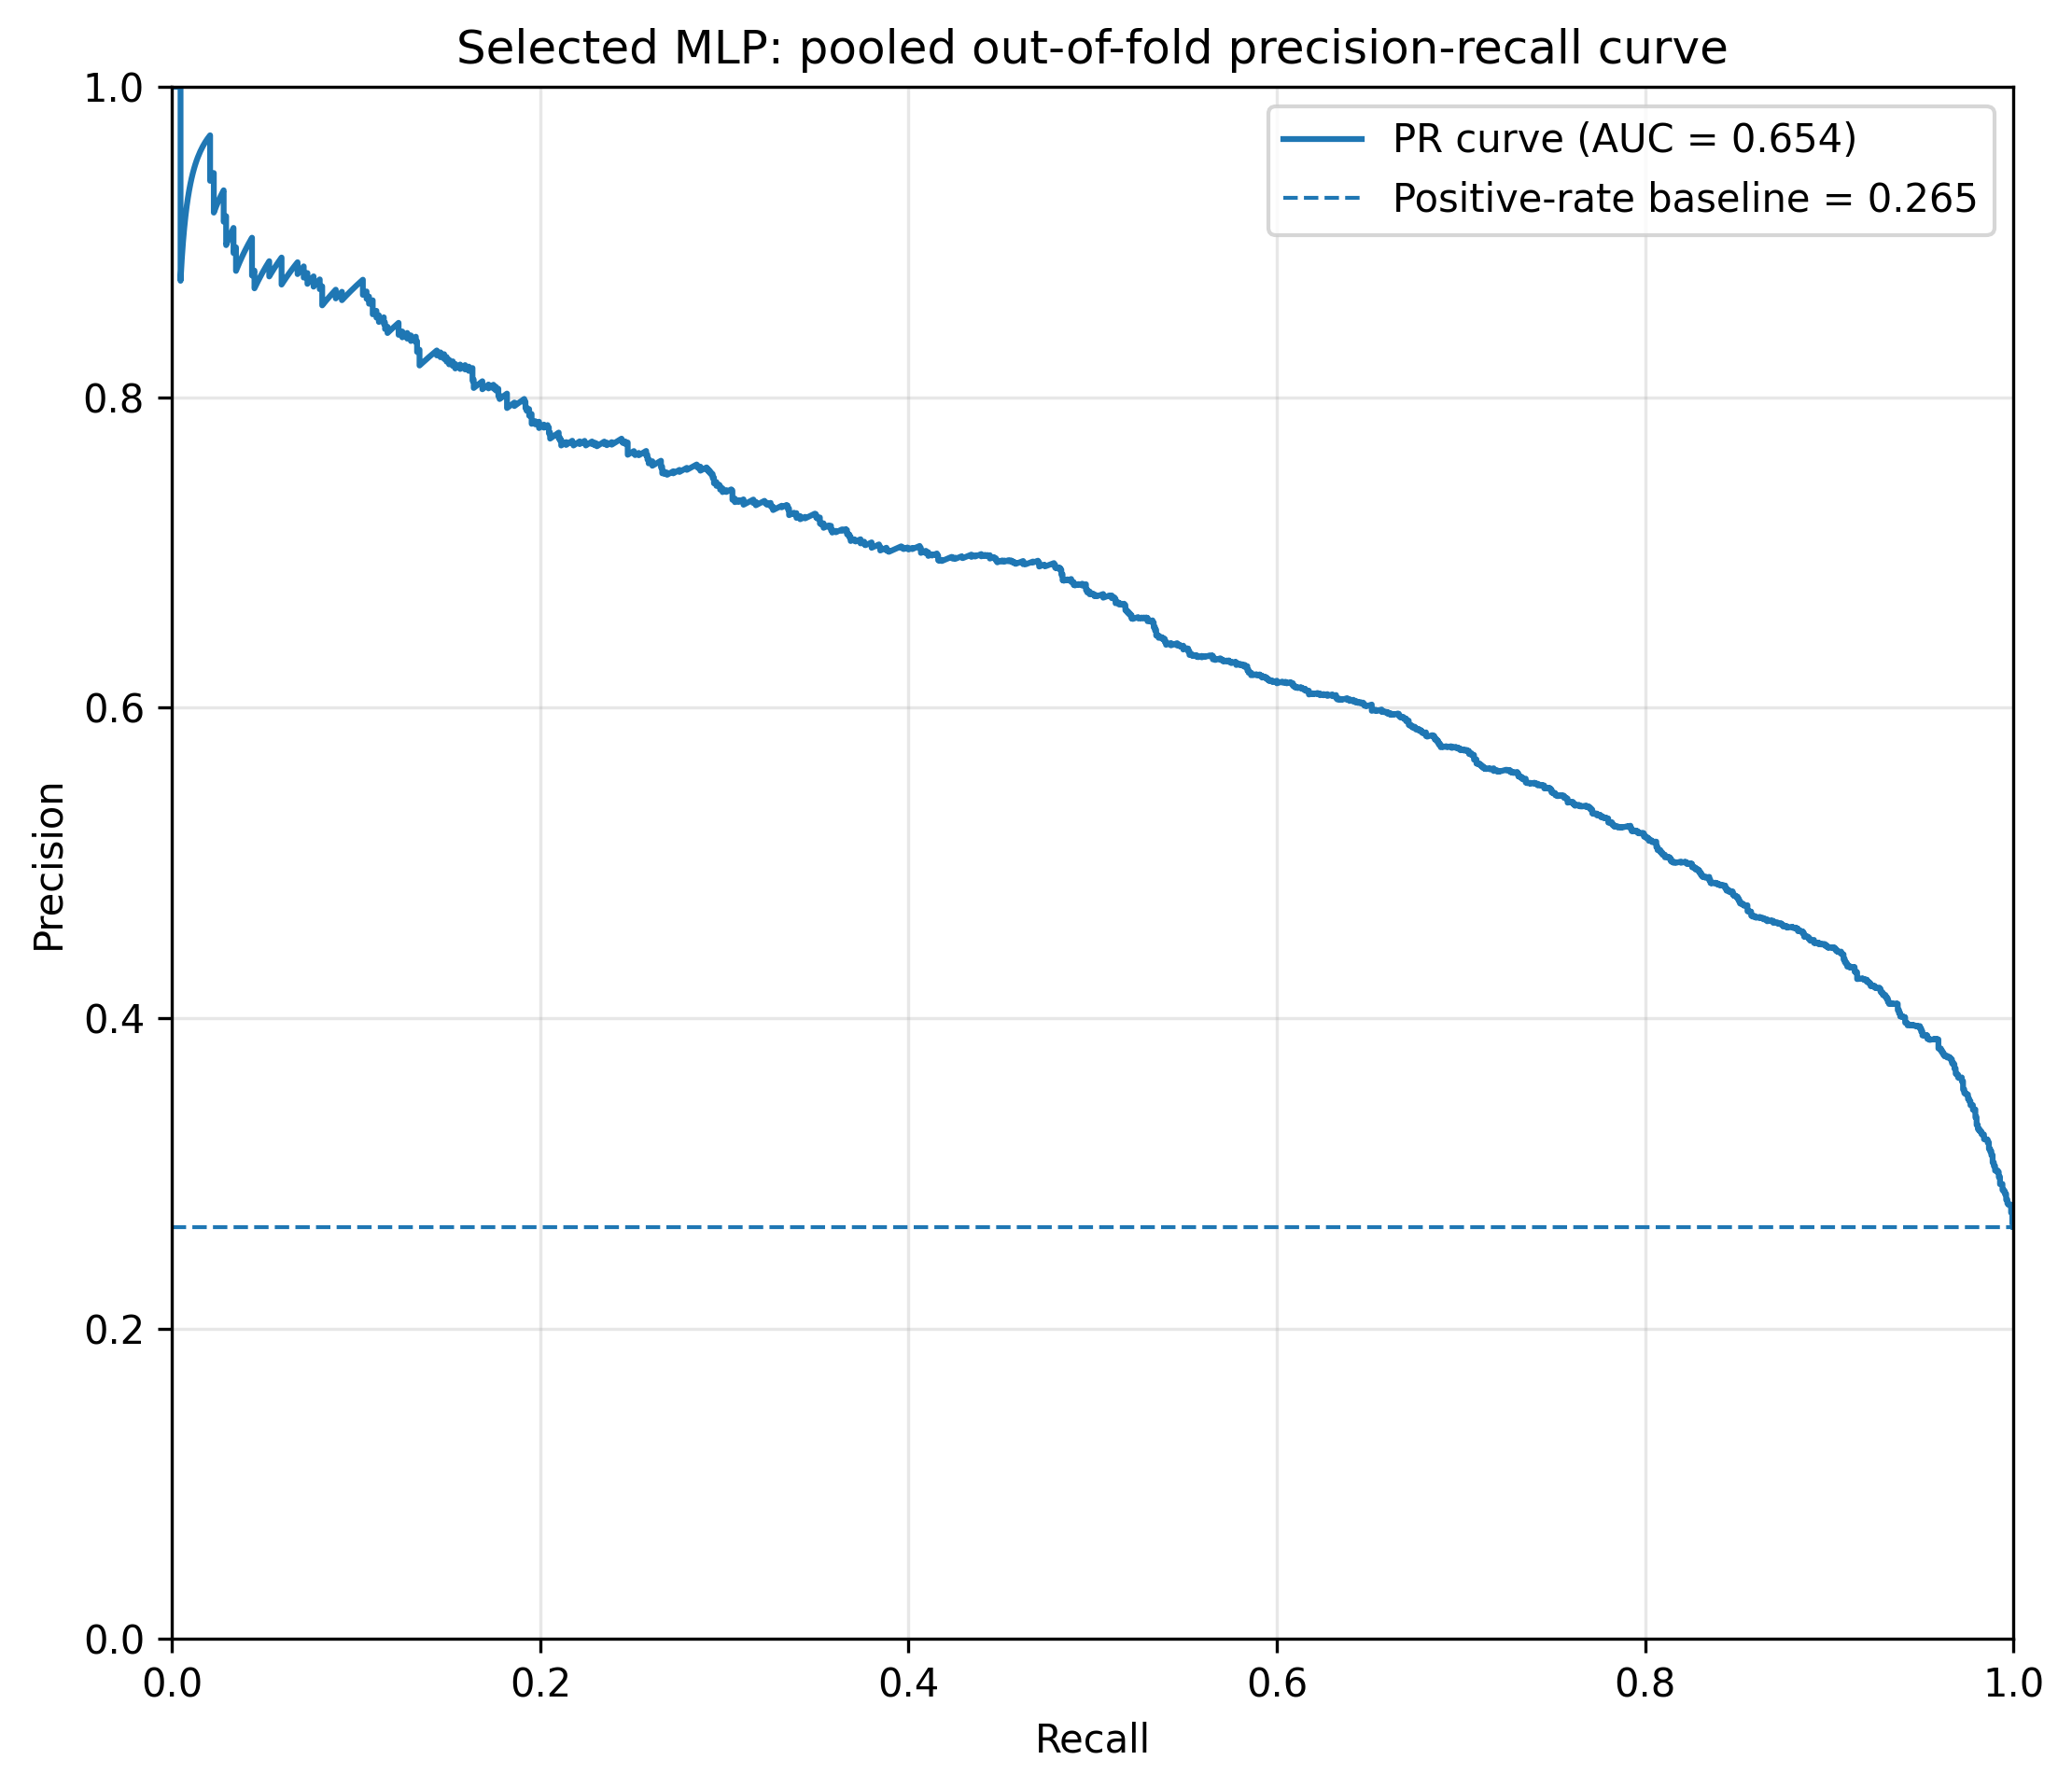
\includegraphics[width=0.82\textwidth]{../figures/mlp_precision_recall_curve.png}
\caption{Precision--recall curve for the selected MLP using pooled out-of-fold churn probabilities}
\label{fig:mlp-pr-curve}
\end{figure}

The PR curve remains materially above the positive-rate baseline of \(0.265\), showing useful churn-risk ranking. However, the observed PR-AUC does not establish a material nonlinear advantage over the project’s strong linear and tree-based references. That question requires fair finalist comparison after all model-family work is complete.

Figure~\ref{fig:mlp-probability-distribution} provides a complementary view of the score distribution. Observed churners are shifted toward larger predicted probabilities, whereas observed non-churners are concentrated near zero. The substantial overlap is expected in a realistic churn task and explains why no fixed threshold simultaneously obtains both very high precision and very high recall.

\begin{figure}[H]
\centering
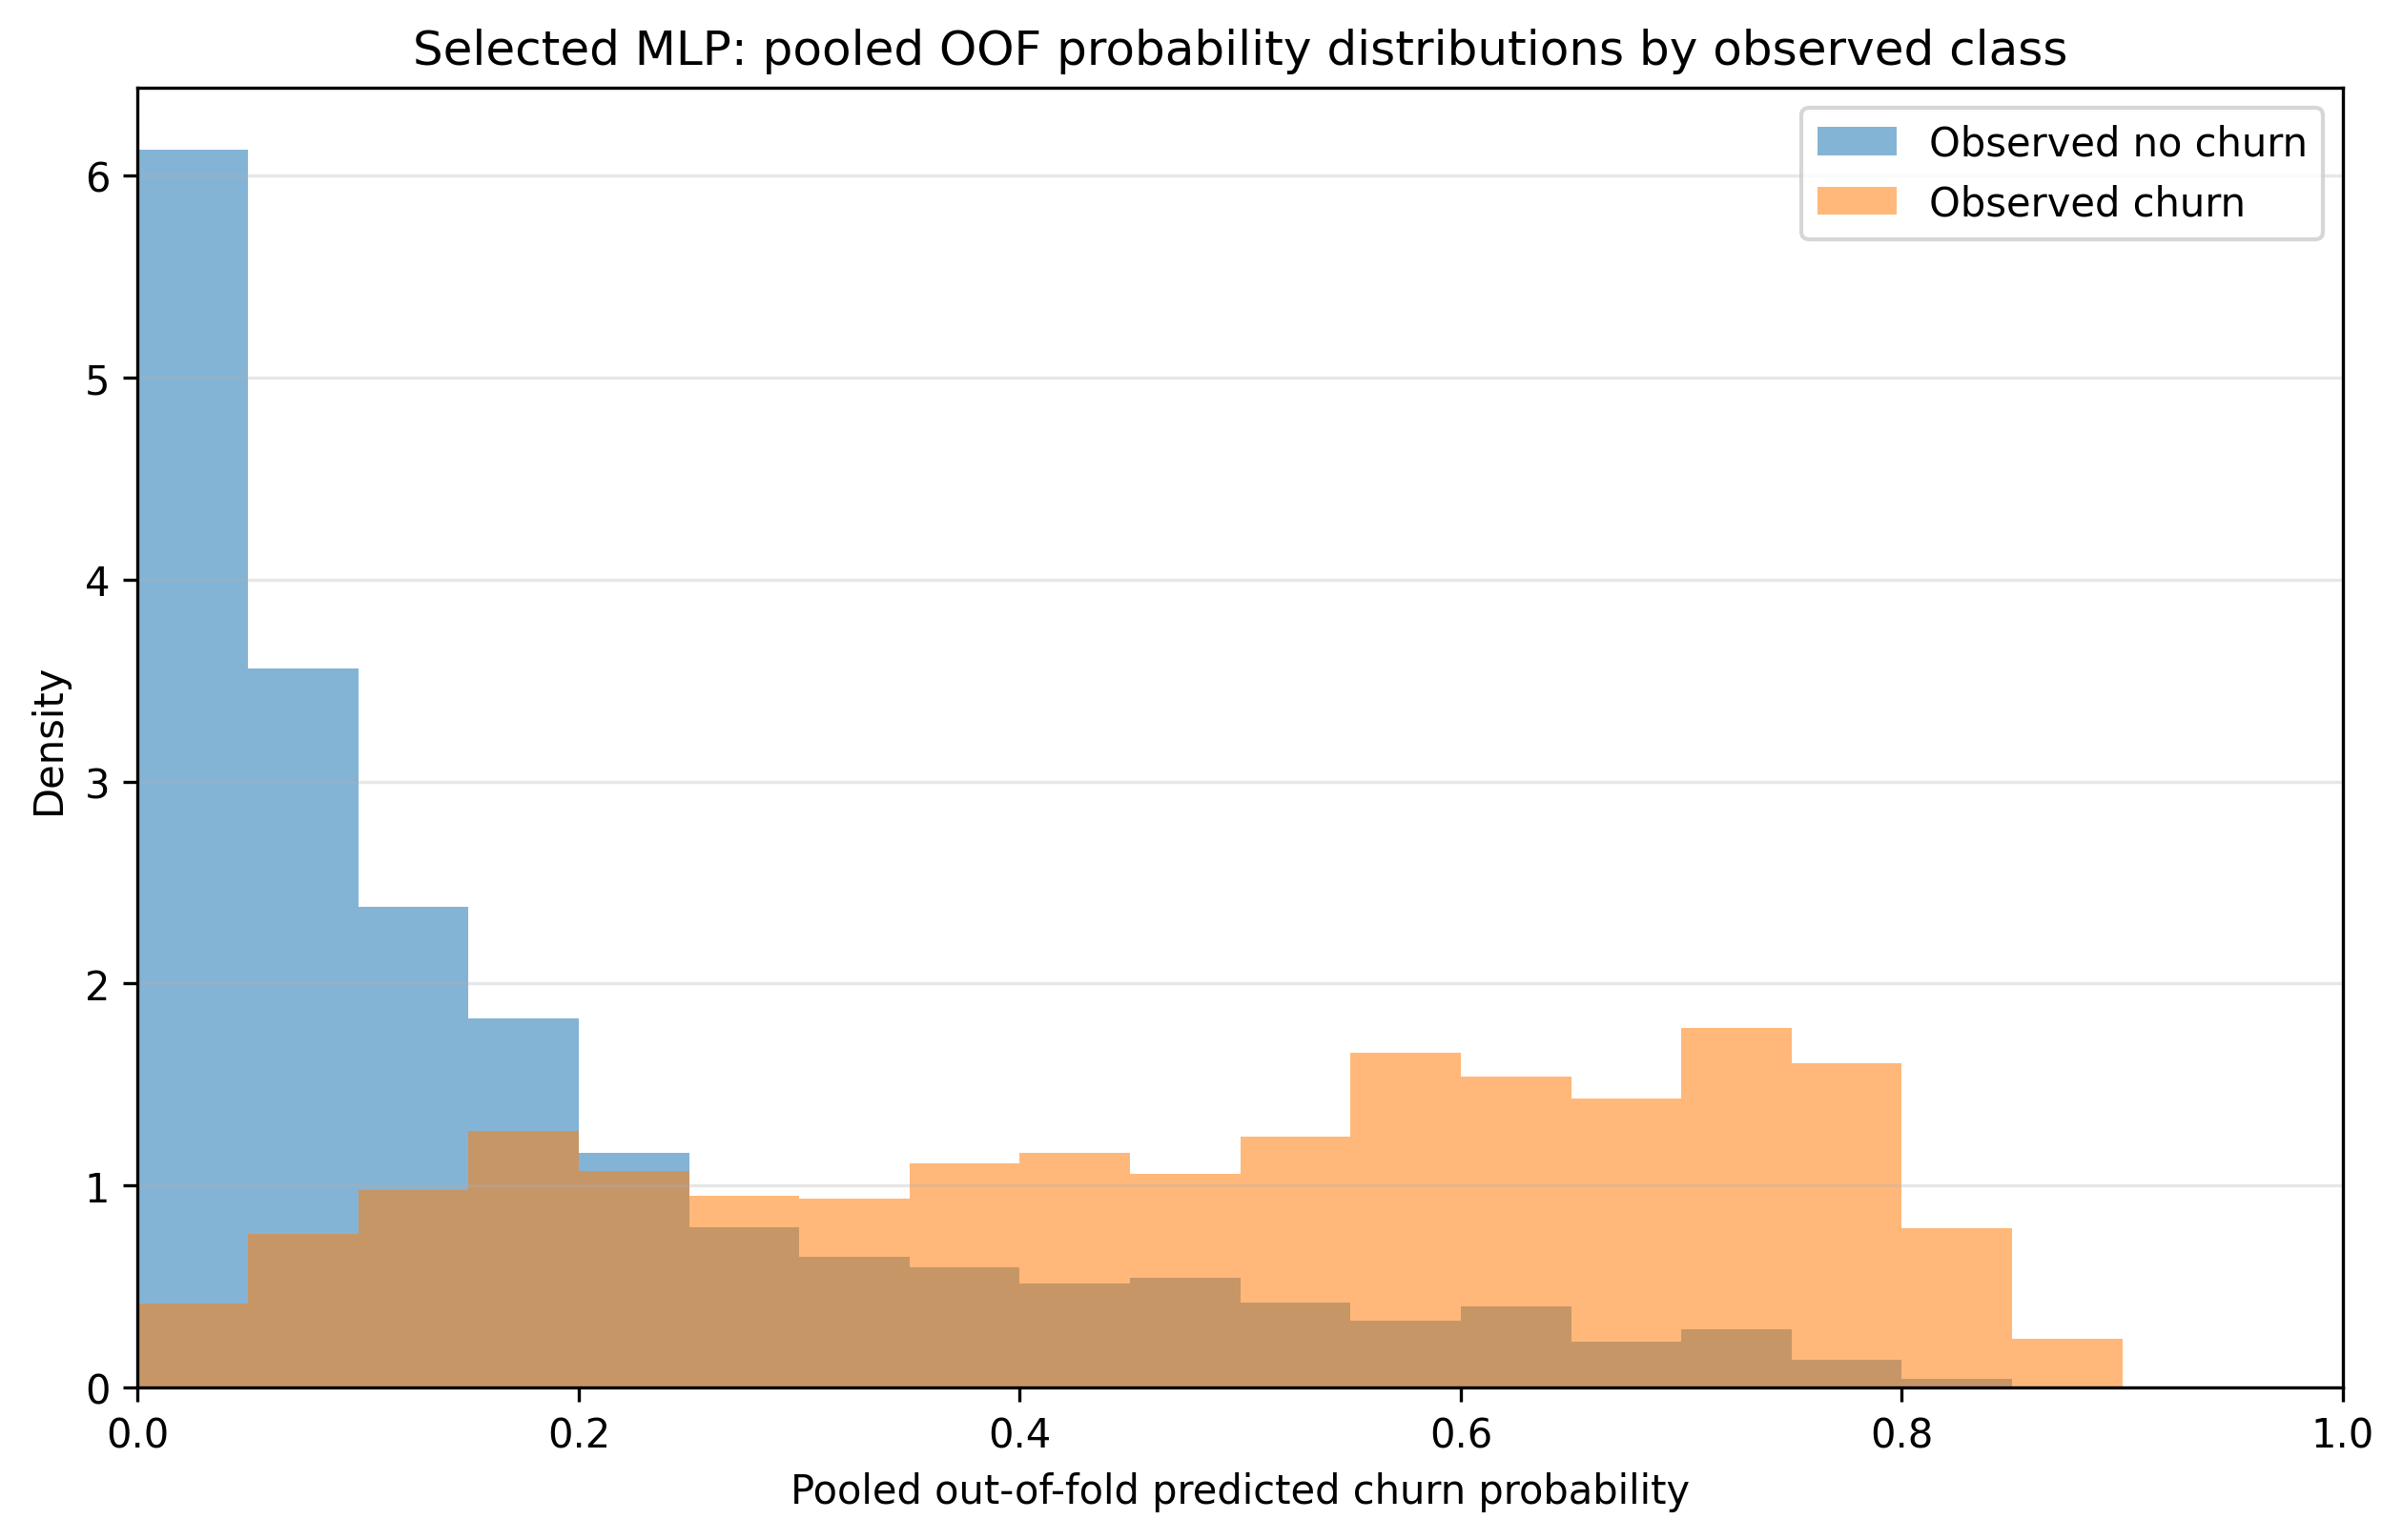
\includegraphics[width=0.88\textwidth]{../figures/mlp_oof_probability_distribution.png}
\caption{Pooled out-of-fold churn-probability distributions by observed class for the selected MLP}
\label{fig:mlp-probability-distribution}
\end{figure}

\subsection{Threshold behaviour and operating-point tradeoffs}

Because the MLP produces probabilities, its threshold has a direct operational interpretation only to the extent that calibration is adequate. Lowering the threshold identifies more potential churners, but increases the intervention list and false-positive rate. Table~\ref{tab:mlp-thresholds} shows selected thresholds calculated from the pooled OOF probabilities.

Within the displayed grid, a threshold of \(0.30\) has the largest \(F_1\), \(0.632\). A threshold of \(0.25\) has the largest displayed balanced accuracy, \(0.764\). Neither value should be adopted as a final production rule here. Both were inspected on the same training-only development evidence used for model selection, and the eventual threshold must depend on intervention capacity, retention value, and the relative cost of missed churners and unnecessary contacts.

\begin{table}[H]
\centering
\small
\begin{tabular}{rrrrrr}
\toprule
Threshold & Precision & Recall & Specificity & \(F_1\) & Pred. positive rate \\
\midrule
0.10 & 0.397 & 0.941 & 0.484 & 0.559 & 0.629 \\
0.20 & 0.495 & 0.829 & 0.695 & 0.620 & 0.444 \\
0.25 & 0.531 & 0.775 & 0.753 & 0.630 & 0.387 \\
0.30 & 0.559 & 0.728 & 0.792 & 0.632 & 0.346 \\
0.50 & 0.667 & 0.514 & 0.907 & 0.581 & 0.205 \\
0.65 & 0.751 & 0.292 & 0.965 & 0.421 & 0.103 \\
\bottomrule
\end{tabular}
\caption{Selected probability thresholds for the MLP using pooled out-of-fold predictions}
\label{tab:mlp-thresholds}
\end{table}

\begin{figure}[H]
\centering
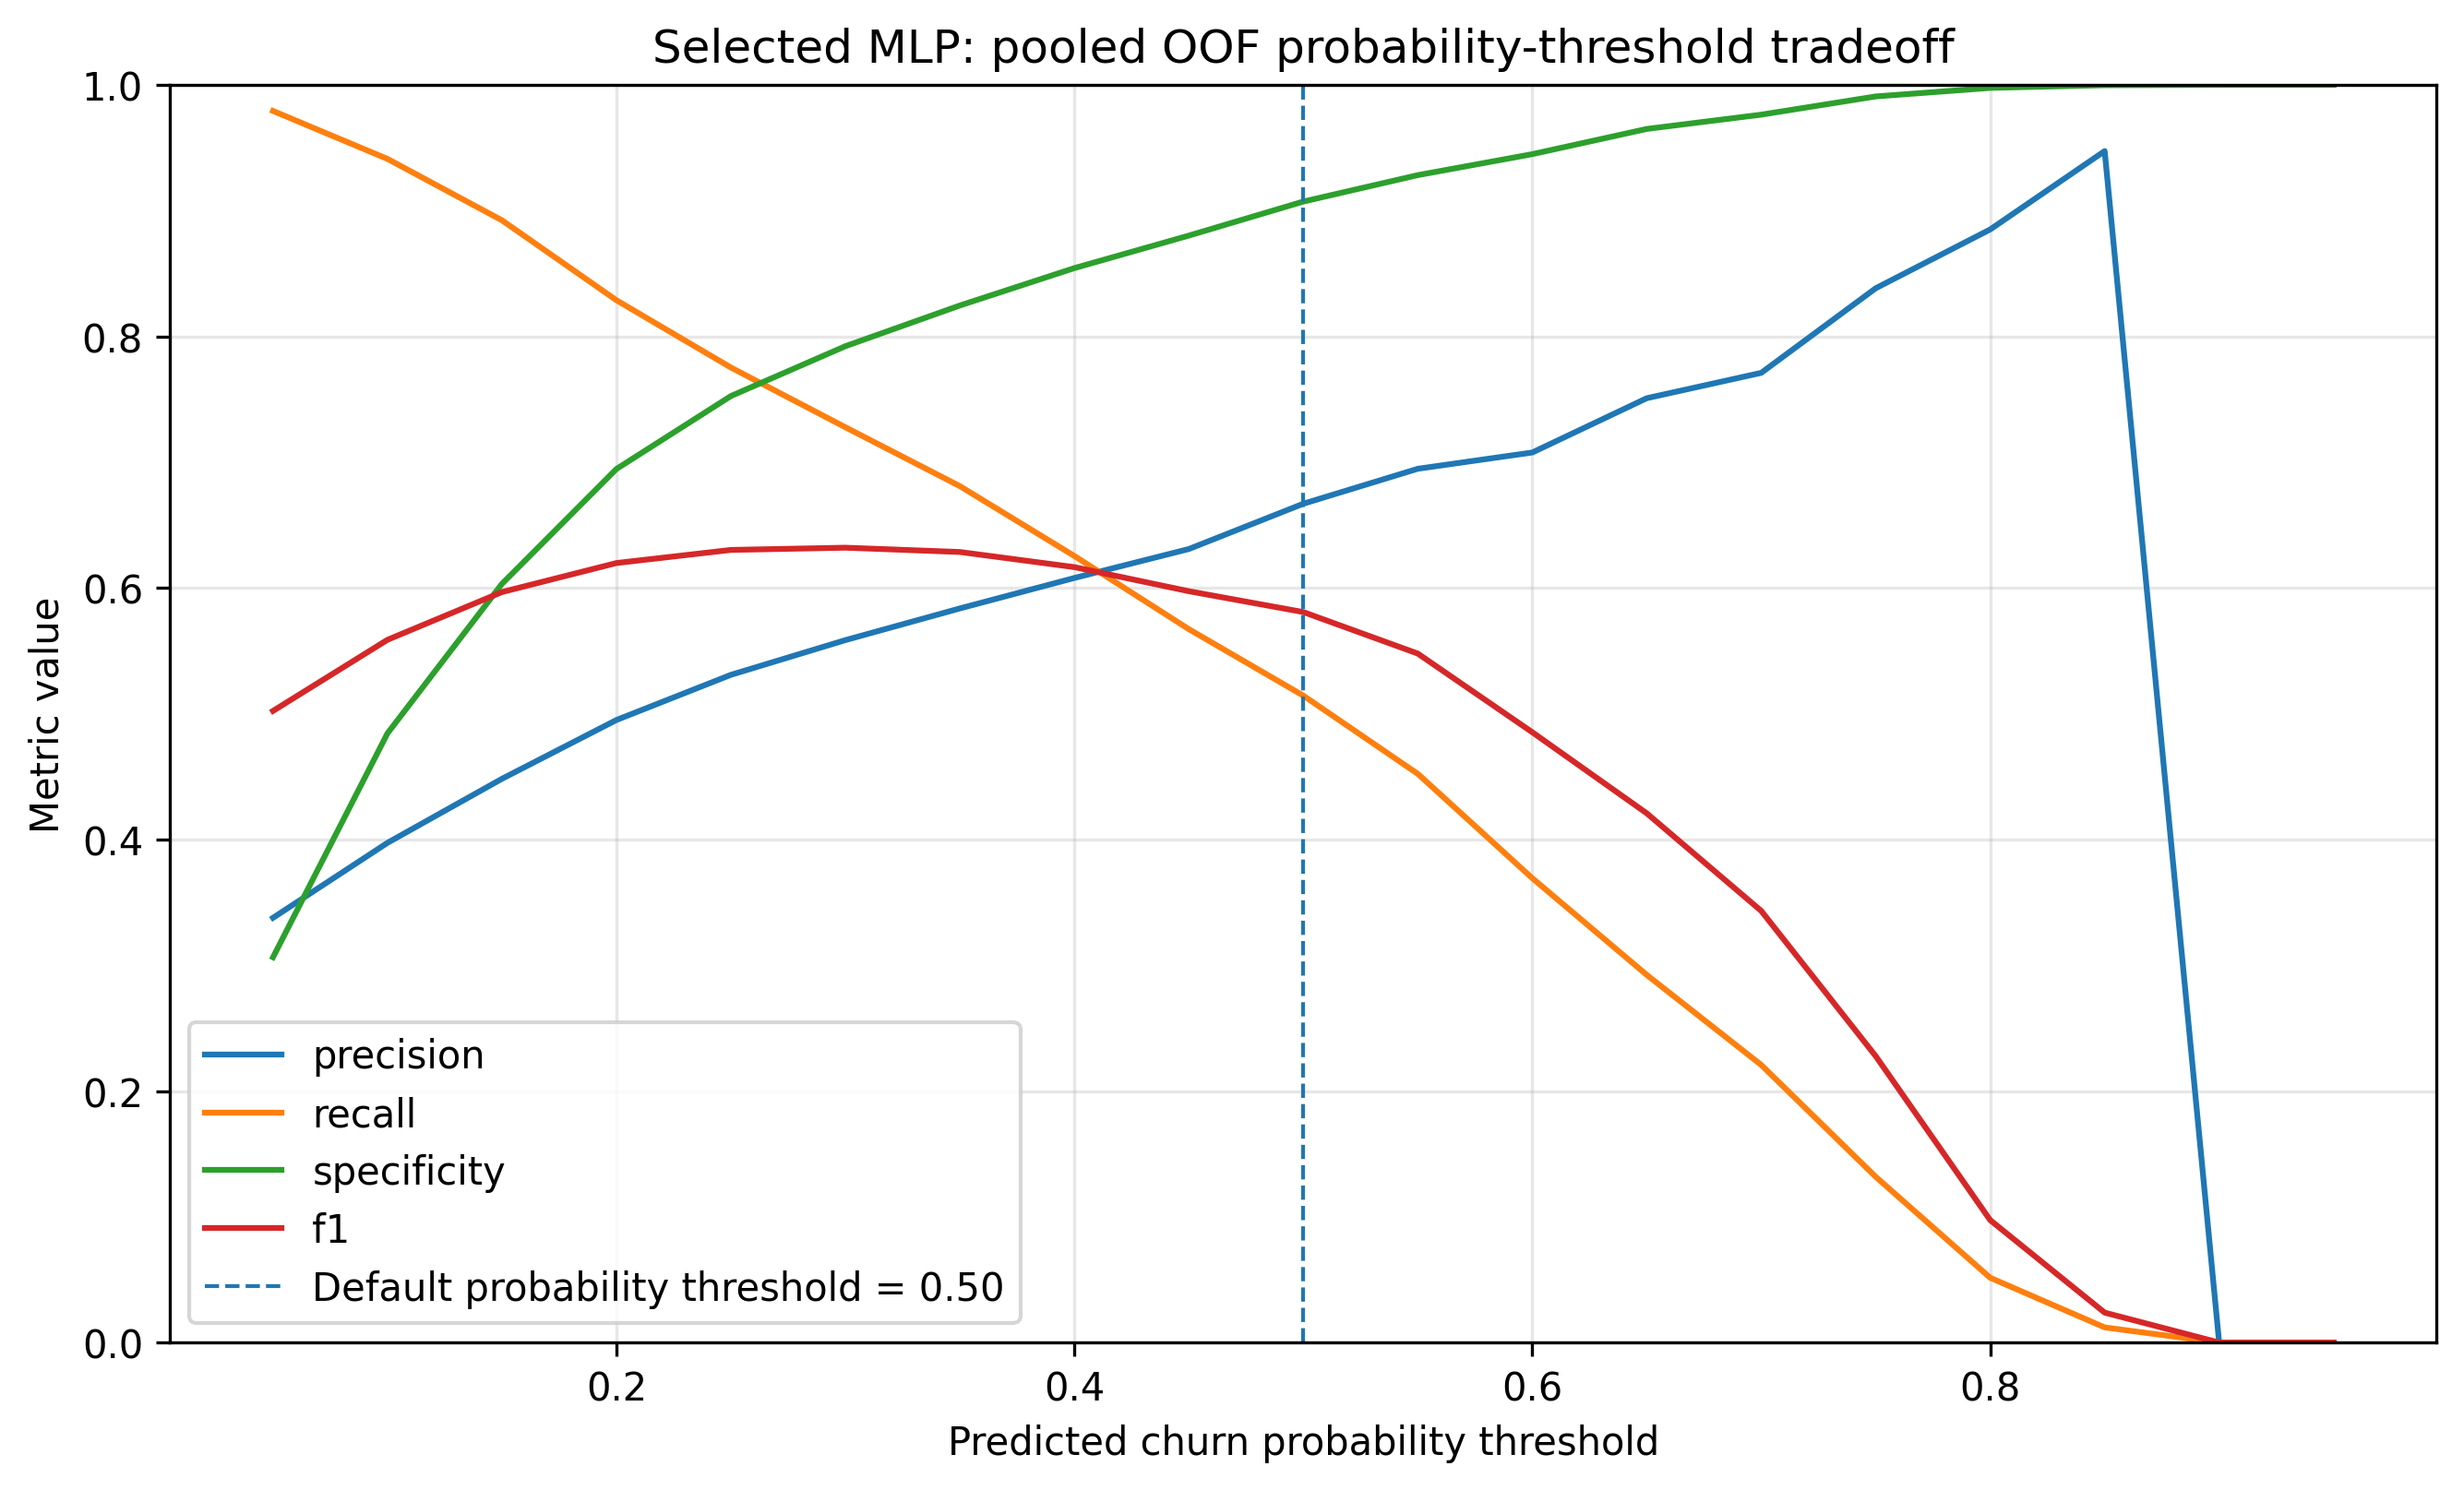
\includegraphics[width=0.88\textwidth]{../figures/mlp_probability_threshold_tradeoff.png}
\caption{Probability-threshold tradeoff for the selected MLP using pooled out-of-fold predictions}
\label{fig:mlp-threshold-tradeoff}
\end{figure}

\subsection{Calibration diagnostic}

The pooled OOF Brier score is \(0.1362\). For context, a non-informative predictor that assigned every customer the observed churn prevalence would have Brier score approximately
\[
\bar{y}(1-\bar{y})
=
0.265(1-0.265)
\approx
0.195.
\]
The selected MLP's mean predicted churn probability is \(0.2588\), close to the observed churn rate \(0.2654\). The ten-bin calibration curve is generally close to the ideal diagonal, although individual bins necessarily have sampling variability.

This is encouraging descriptive evidence, not a declaration that the model is fully calibrated for deployment. Calibration should later be compared systematically across serious finalists, and any calibration transformation must be estimated within a training-only resampling procedure.

\begin{figure}[H]
\centering
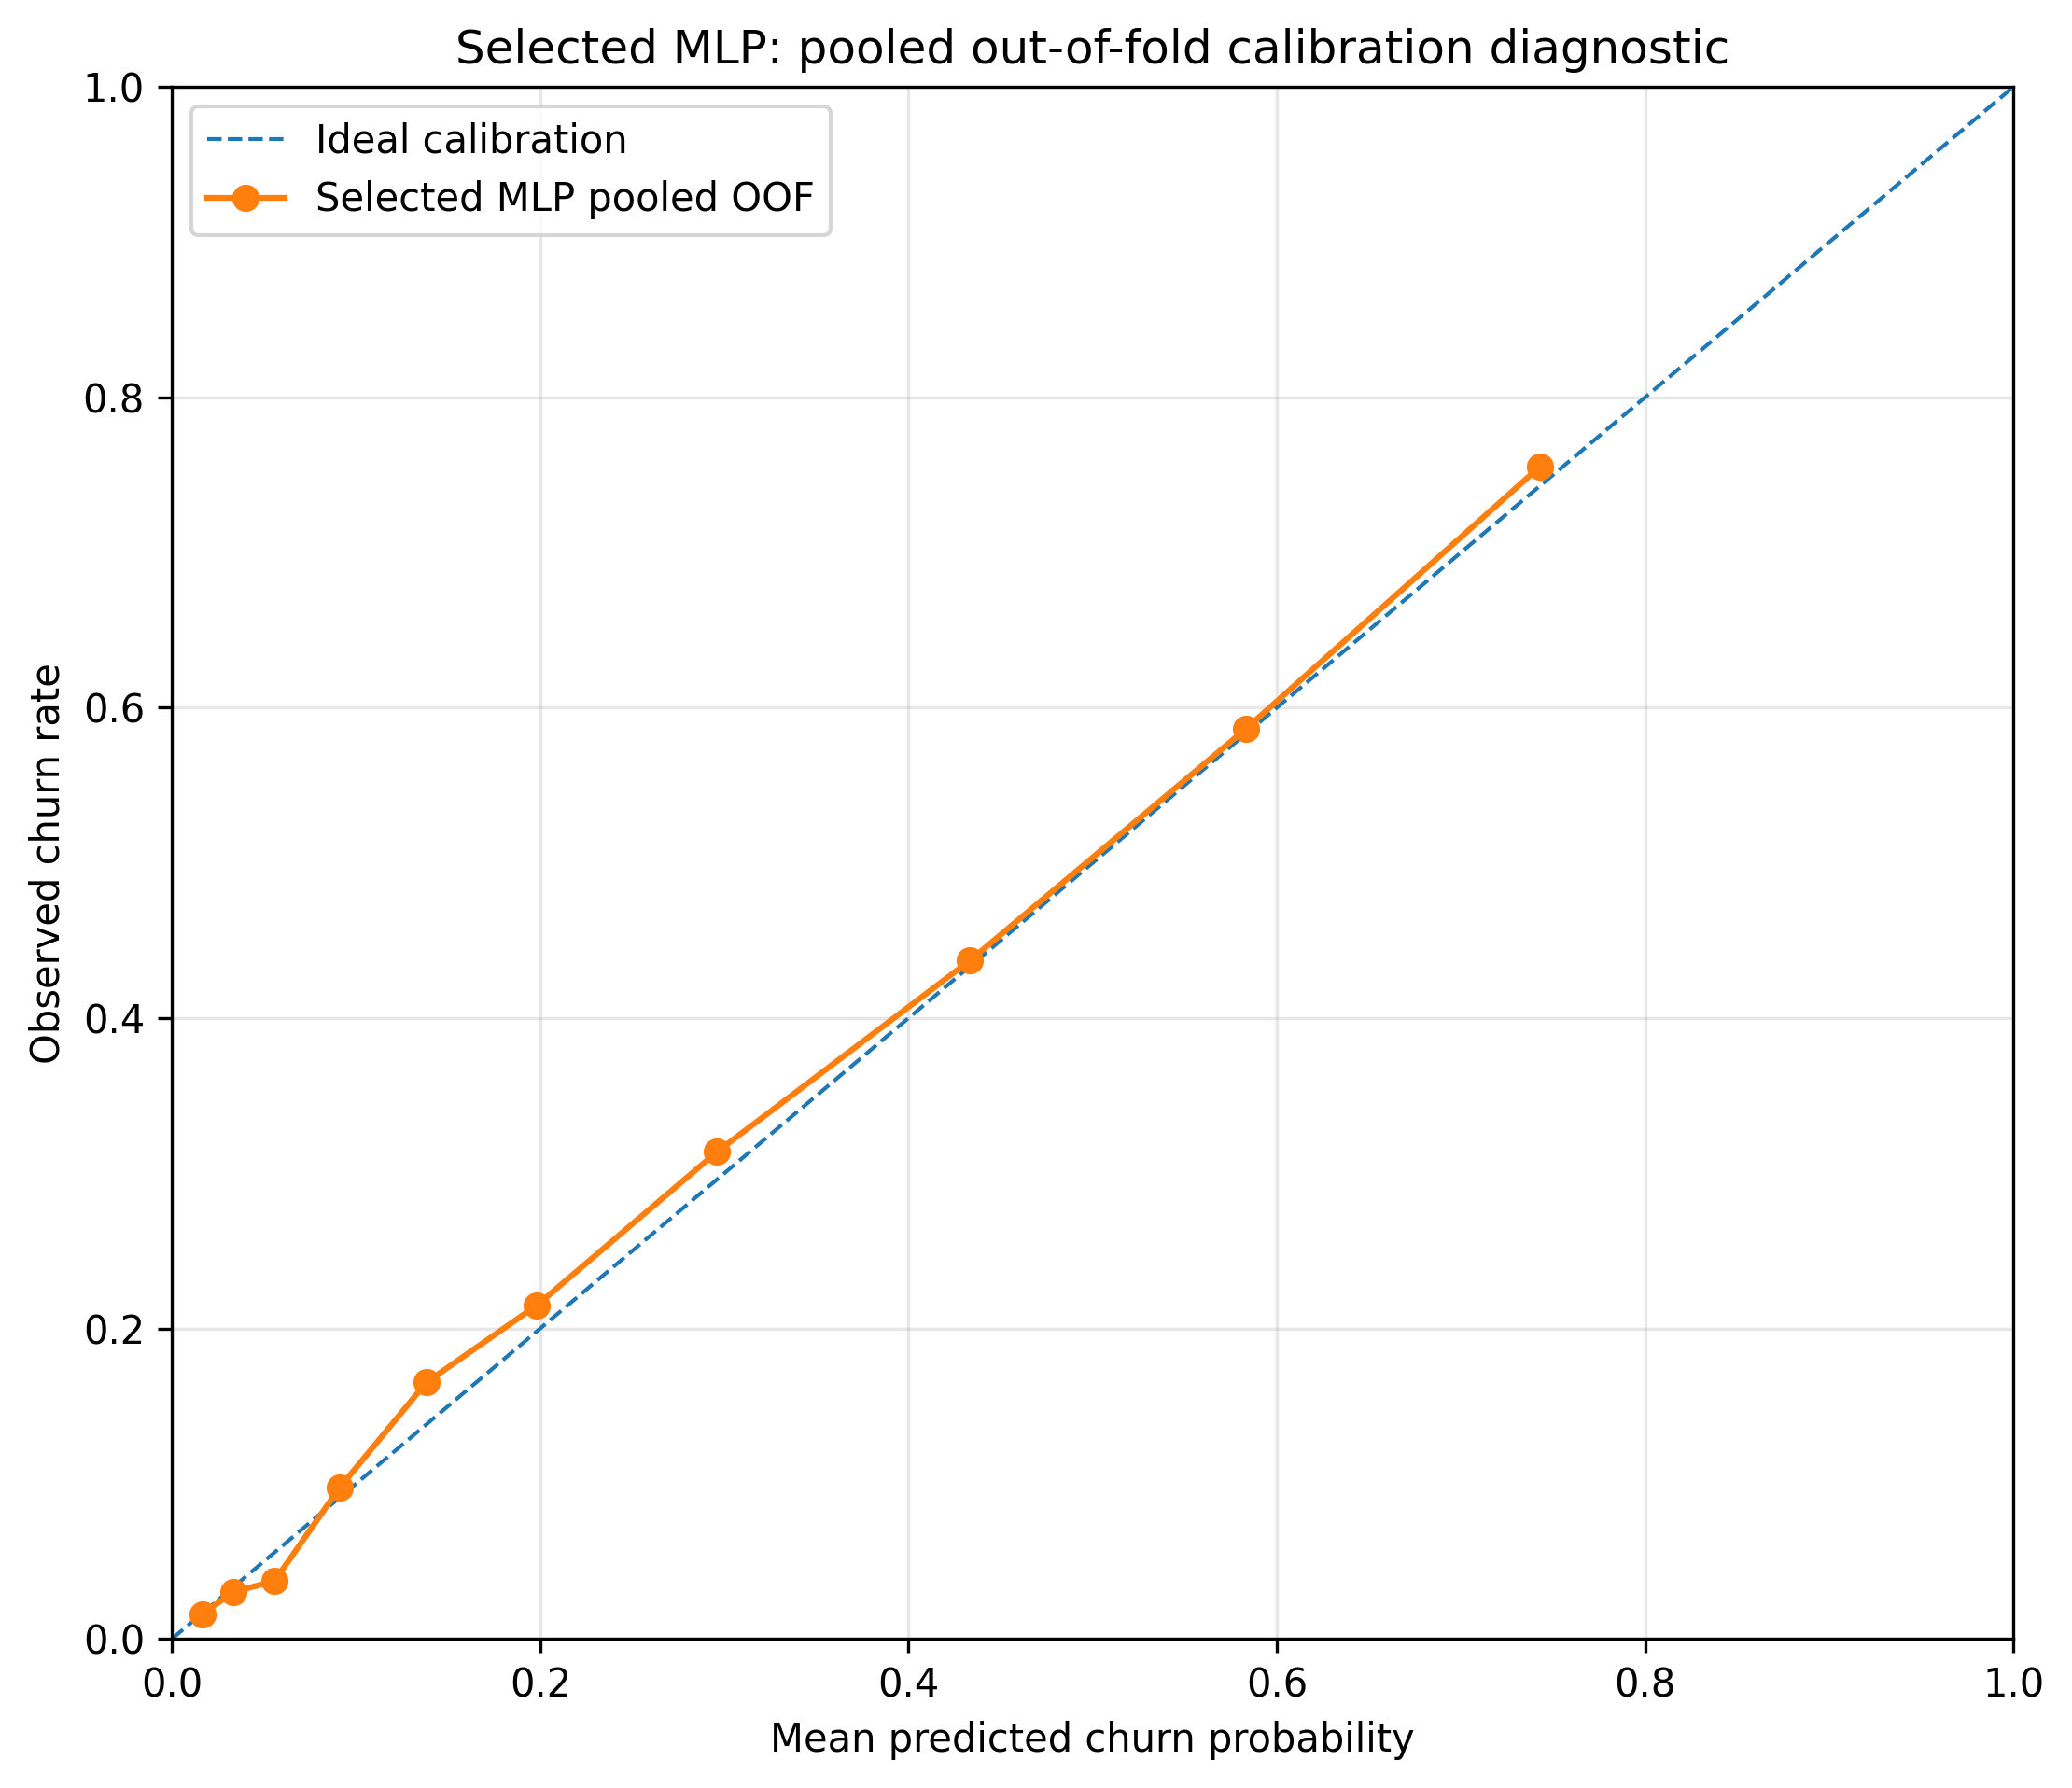
\includegraphics[width=0.82\textwidth]{../figures/mlp_calibration_curve.png}
\caption{Pooled out-of-fold calibration diagnostic for the selected MLP}
\label{fig:mlp-calibration}
\end{figure}

\subsection{Optimization and seed-sensitivity diagnostics}

When the selected pipeline is fitted once on the complete training set for optimization diagnostics, the training loss falls from approximately \(0.585\) in the first epoch to \(0.396\) after \(42\) epochs. The internal validation accuracy fluctuates around \(0.80\) and reaches a maximum of approximately \(0.811\). There are no convergence warnings in the five outer-fold fits or the full-training diagnostic fit.

The full-training curves are not independent performance estimates. Their role is to check that optimization is numerically stable, that the loss decreases, and that early stopping intervenes before a fixed \(500\)-iteration limit is exhausted. They must not replace the outer-fold validation metrics for model comparison.

\begin{figure}[H]
\centering
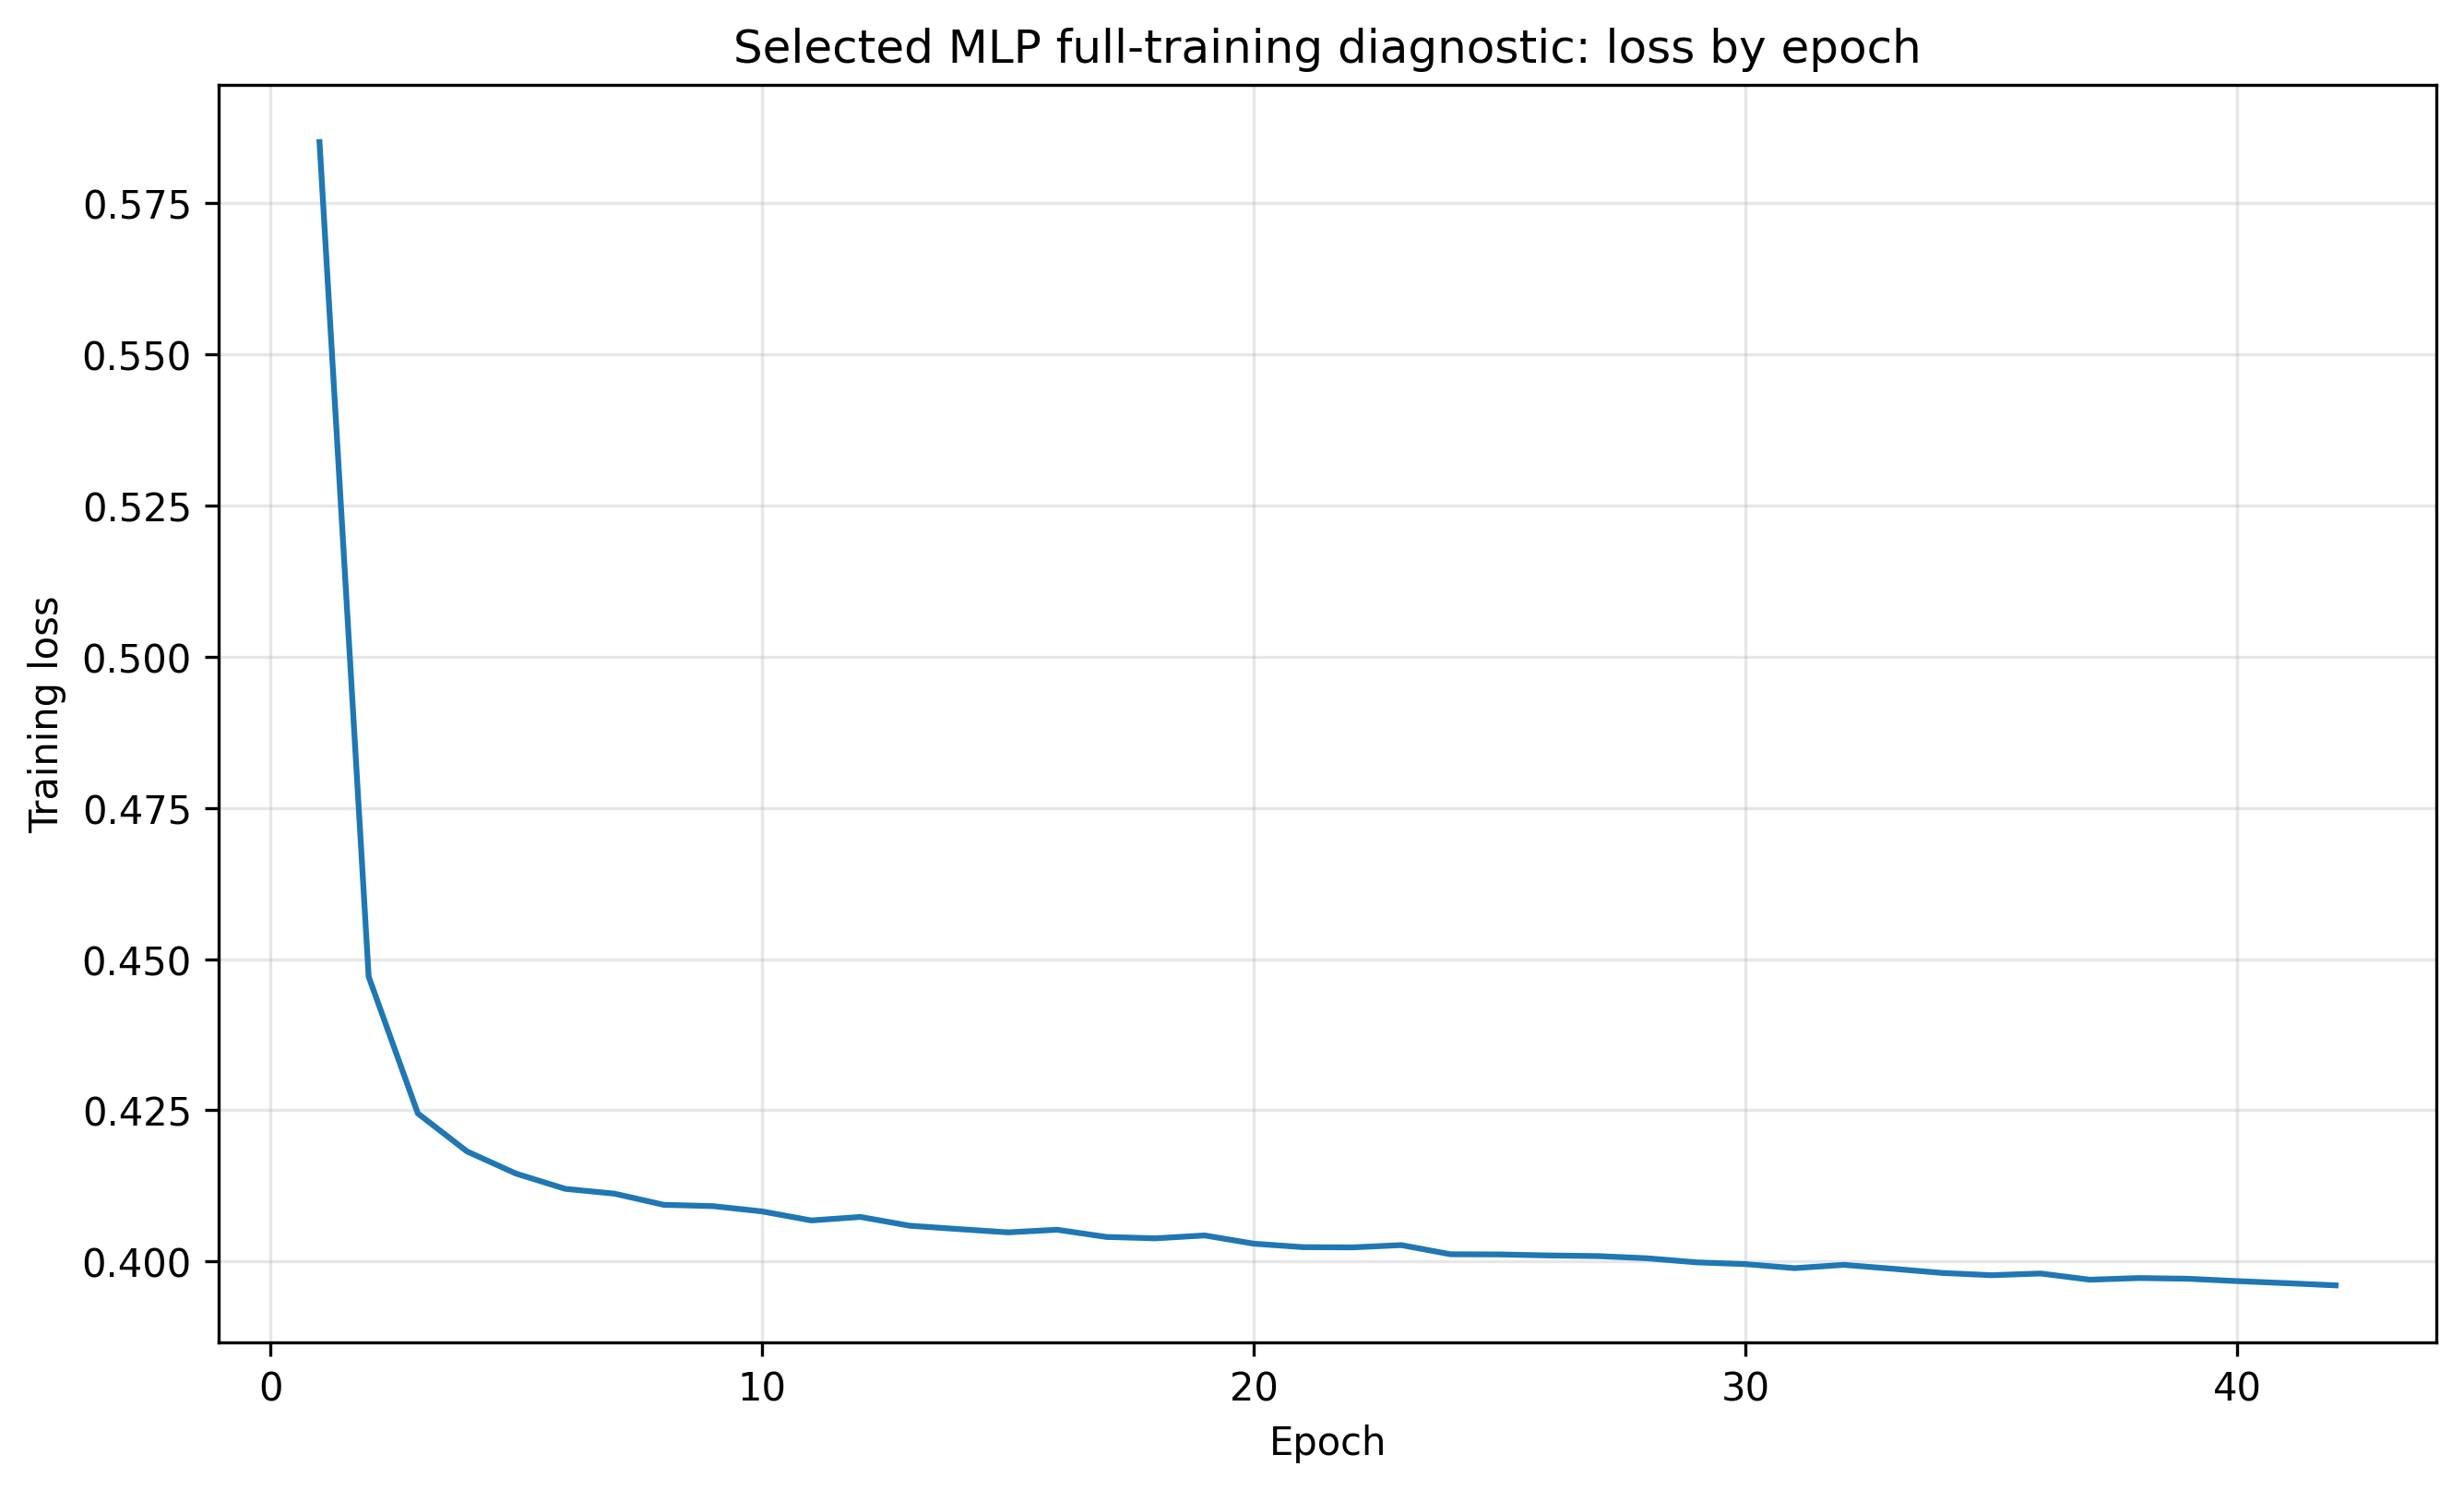
\includegraphics[width=0.82\textwidth]{../figures/mlp_training_loss_curve.png}
\caption{Full-training loss trajectory for the selected MLP diagnostic fit}
\label{fig:mlp-training-loss}
\end{figure}

\begin{figure}[H]
\centering
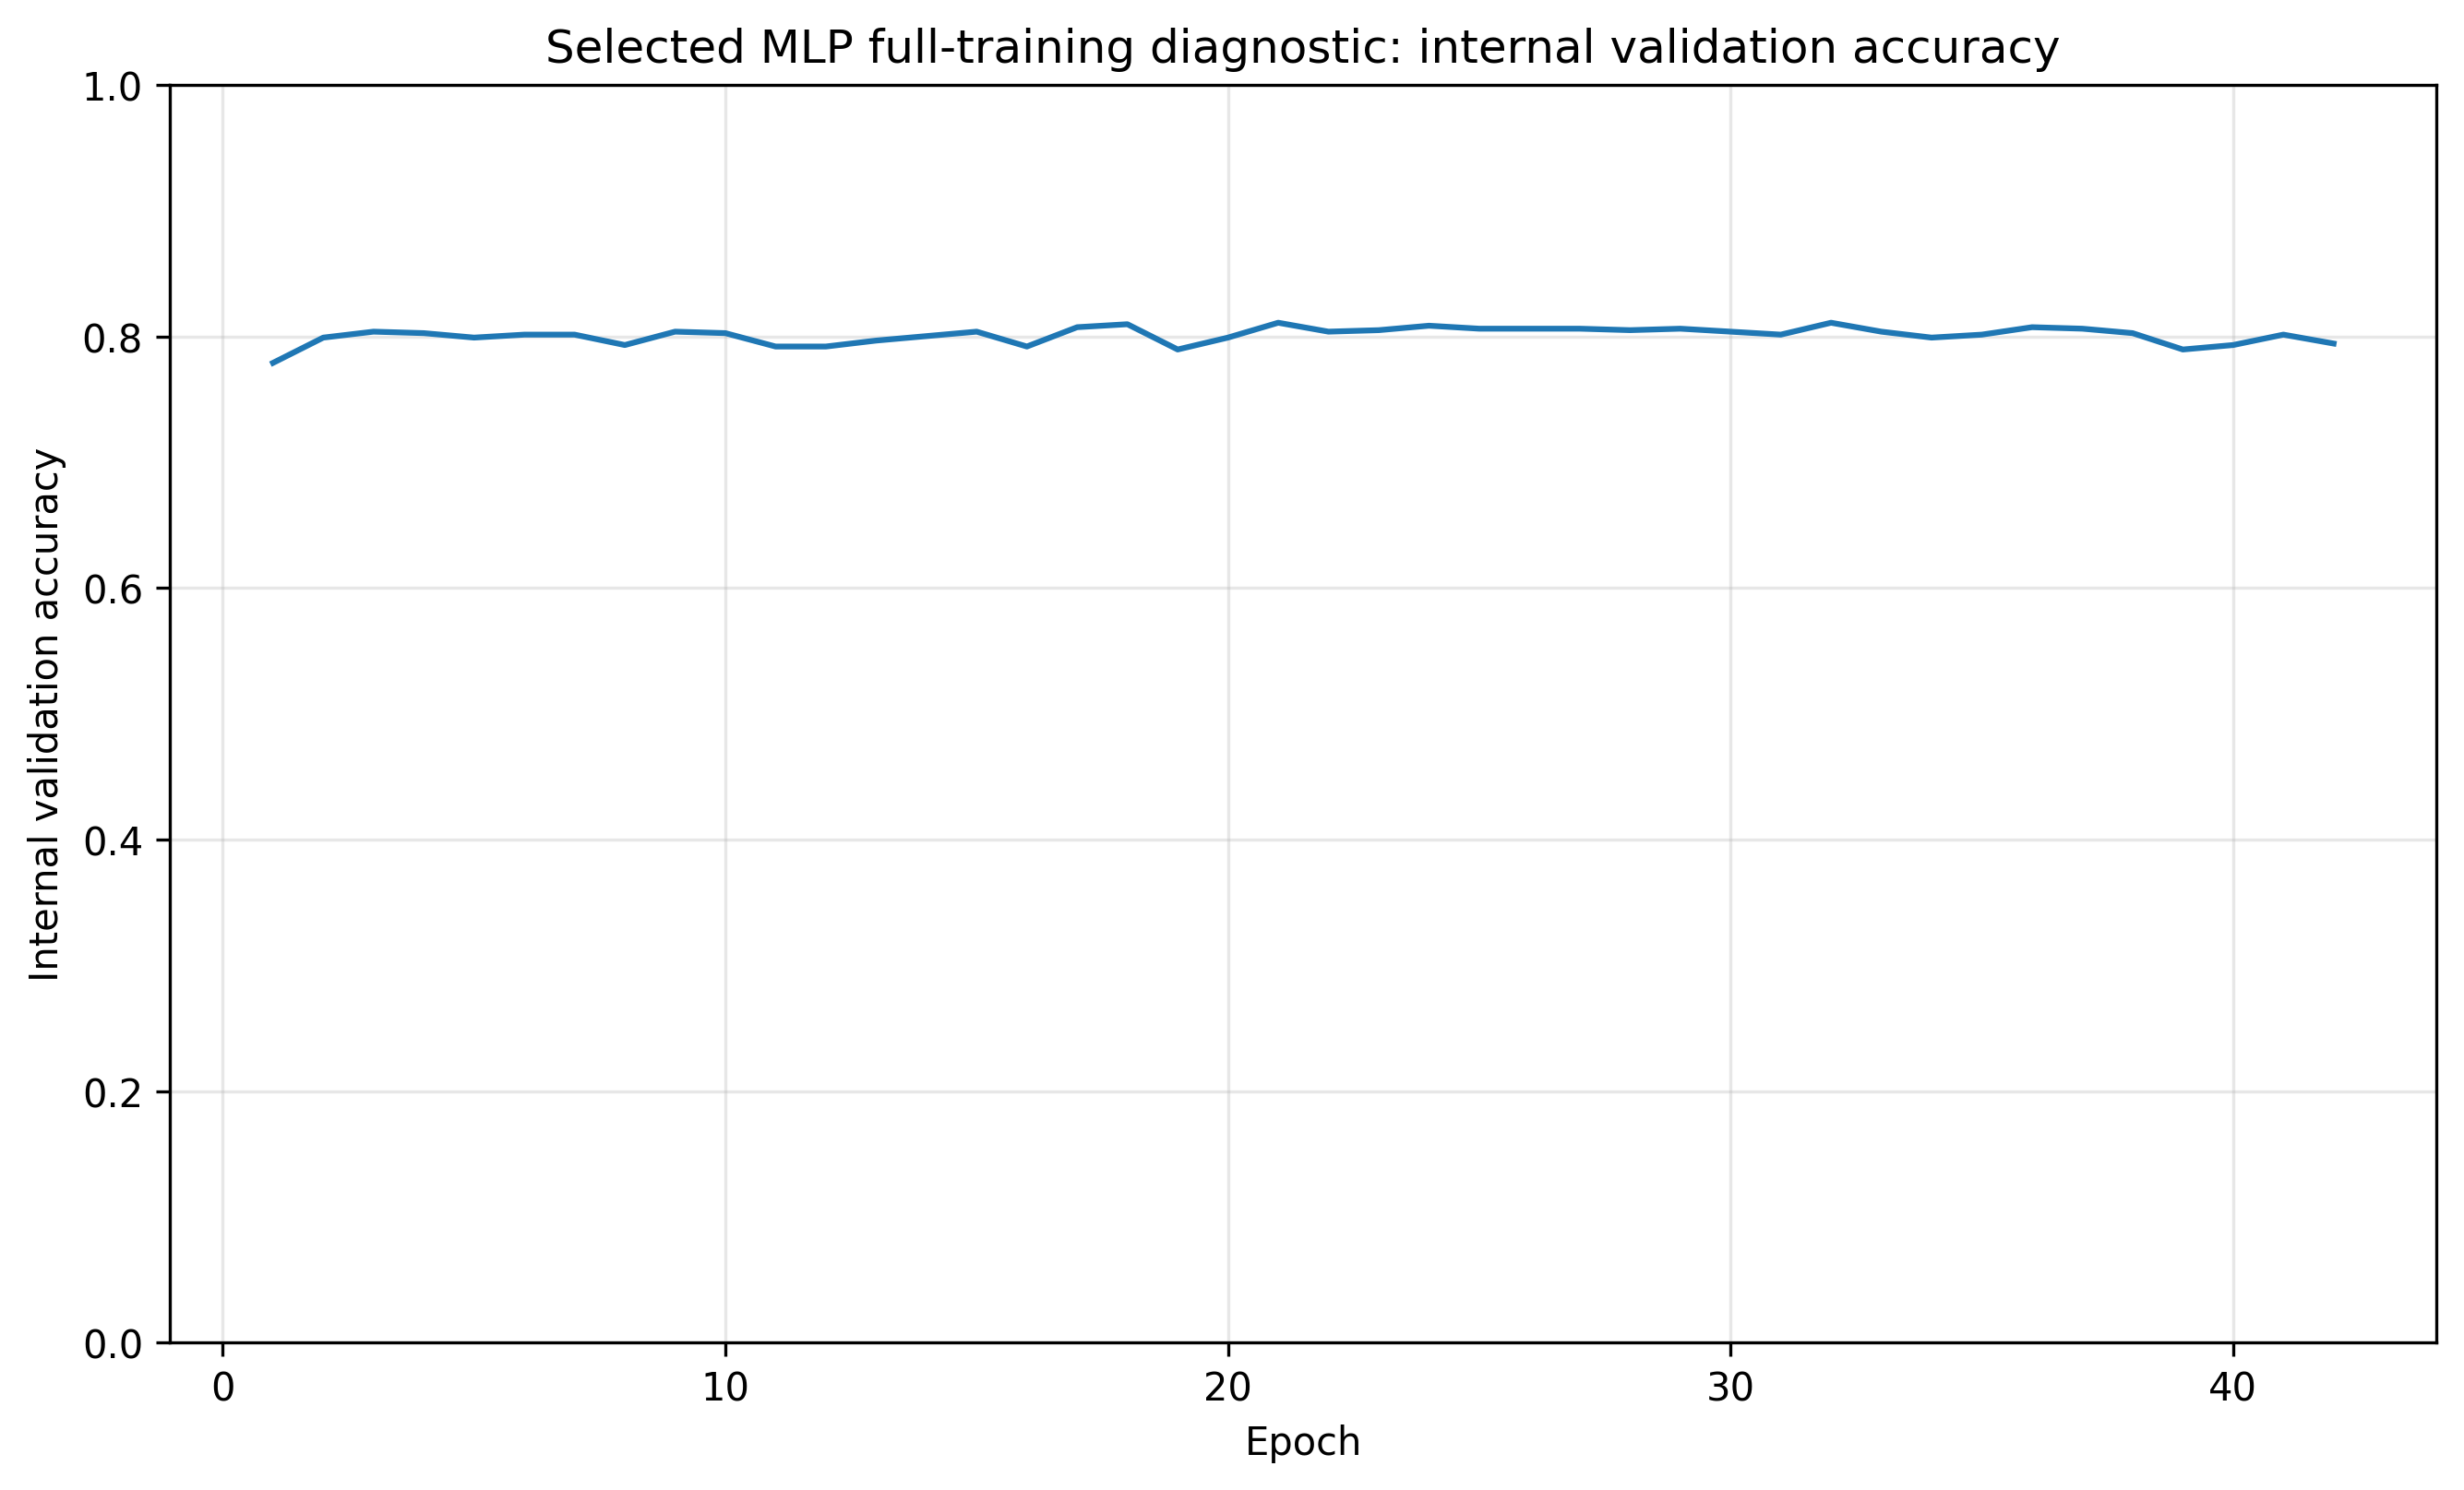
\includegraphics[width=0.82\textwidth]{../figures/mlp_internal_validation_accuracy_curve.png}
\caption{Internal validation-accuracy trajectory for the selected MLP diagnostic fit}
\label{fig:mlp-internal-validation}
\end{figure}

Neural-network fitting is stochastic because of random initialization and minibatch optimization. The selected architecture was therefore re-evaluated across four random states. Pooled OOF PR-AUC ranges from \(0.6502\) to \(0.6554\), with standard deviation approximately \(0.0023\). This is modest variation, but it is large enough to reinforce the general conclusion that small differences among nearby MLP grid configurations should not be treated as decisive.

\begin{figure}[H]
\centering
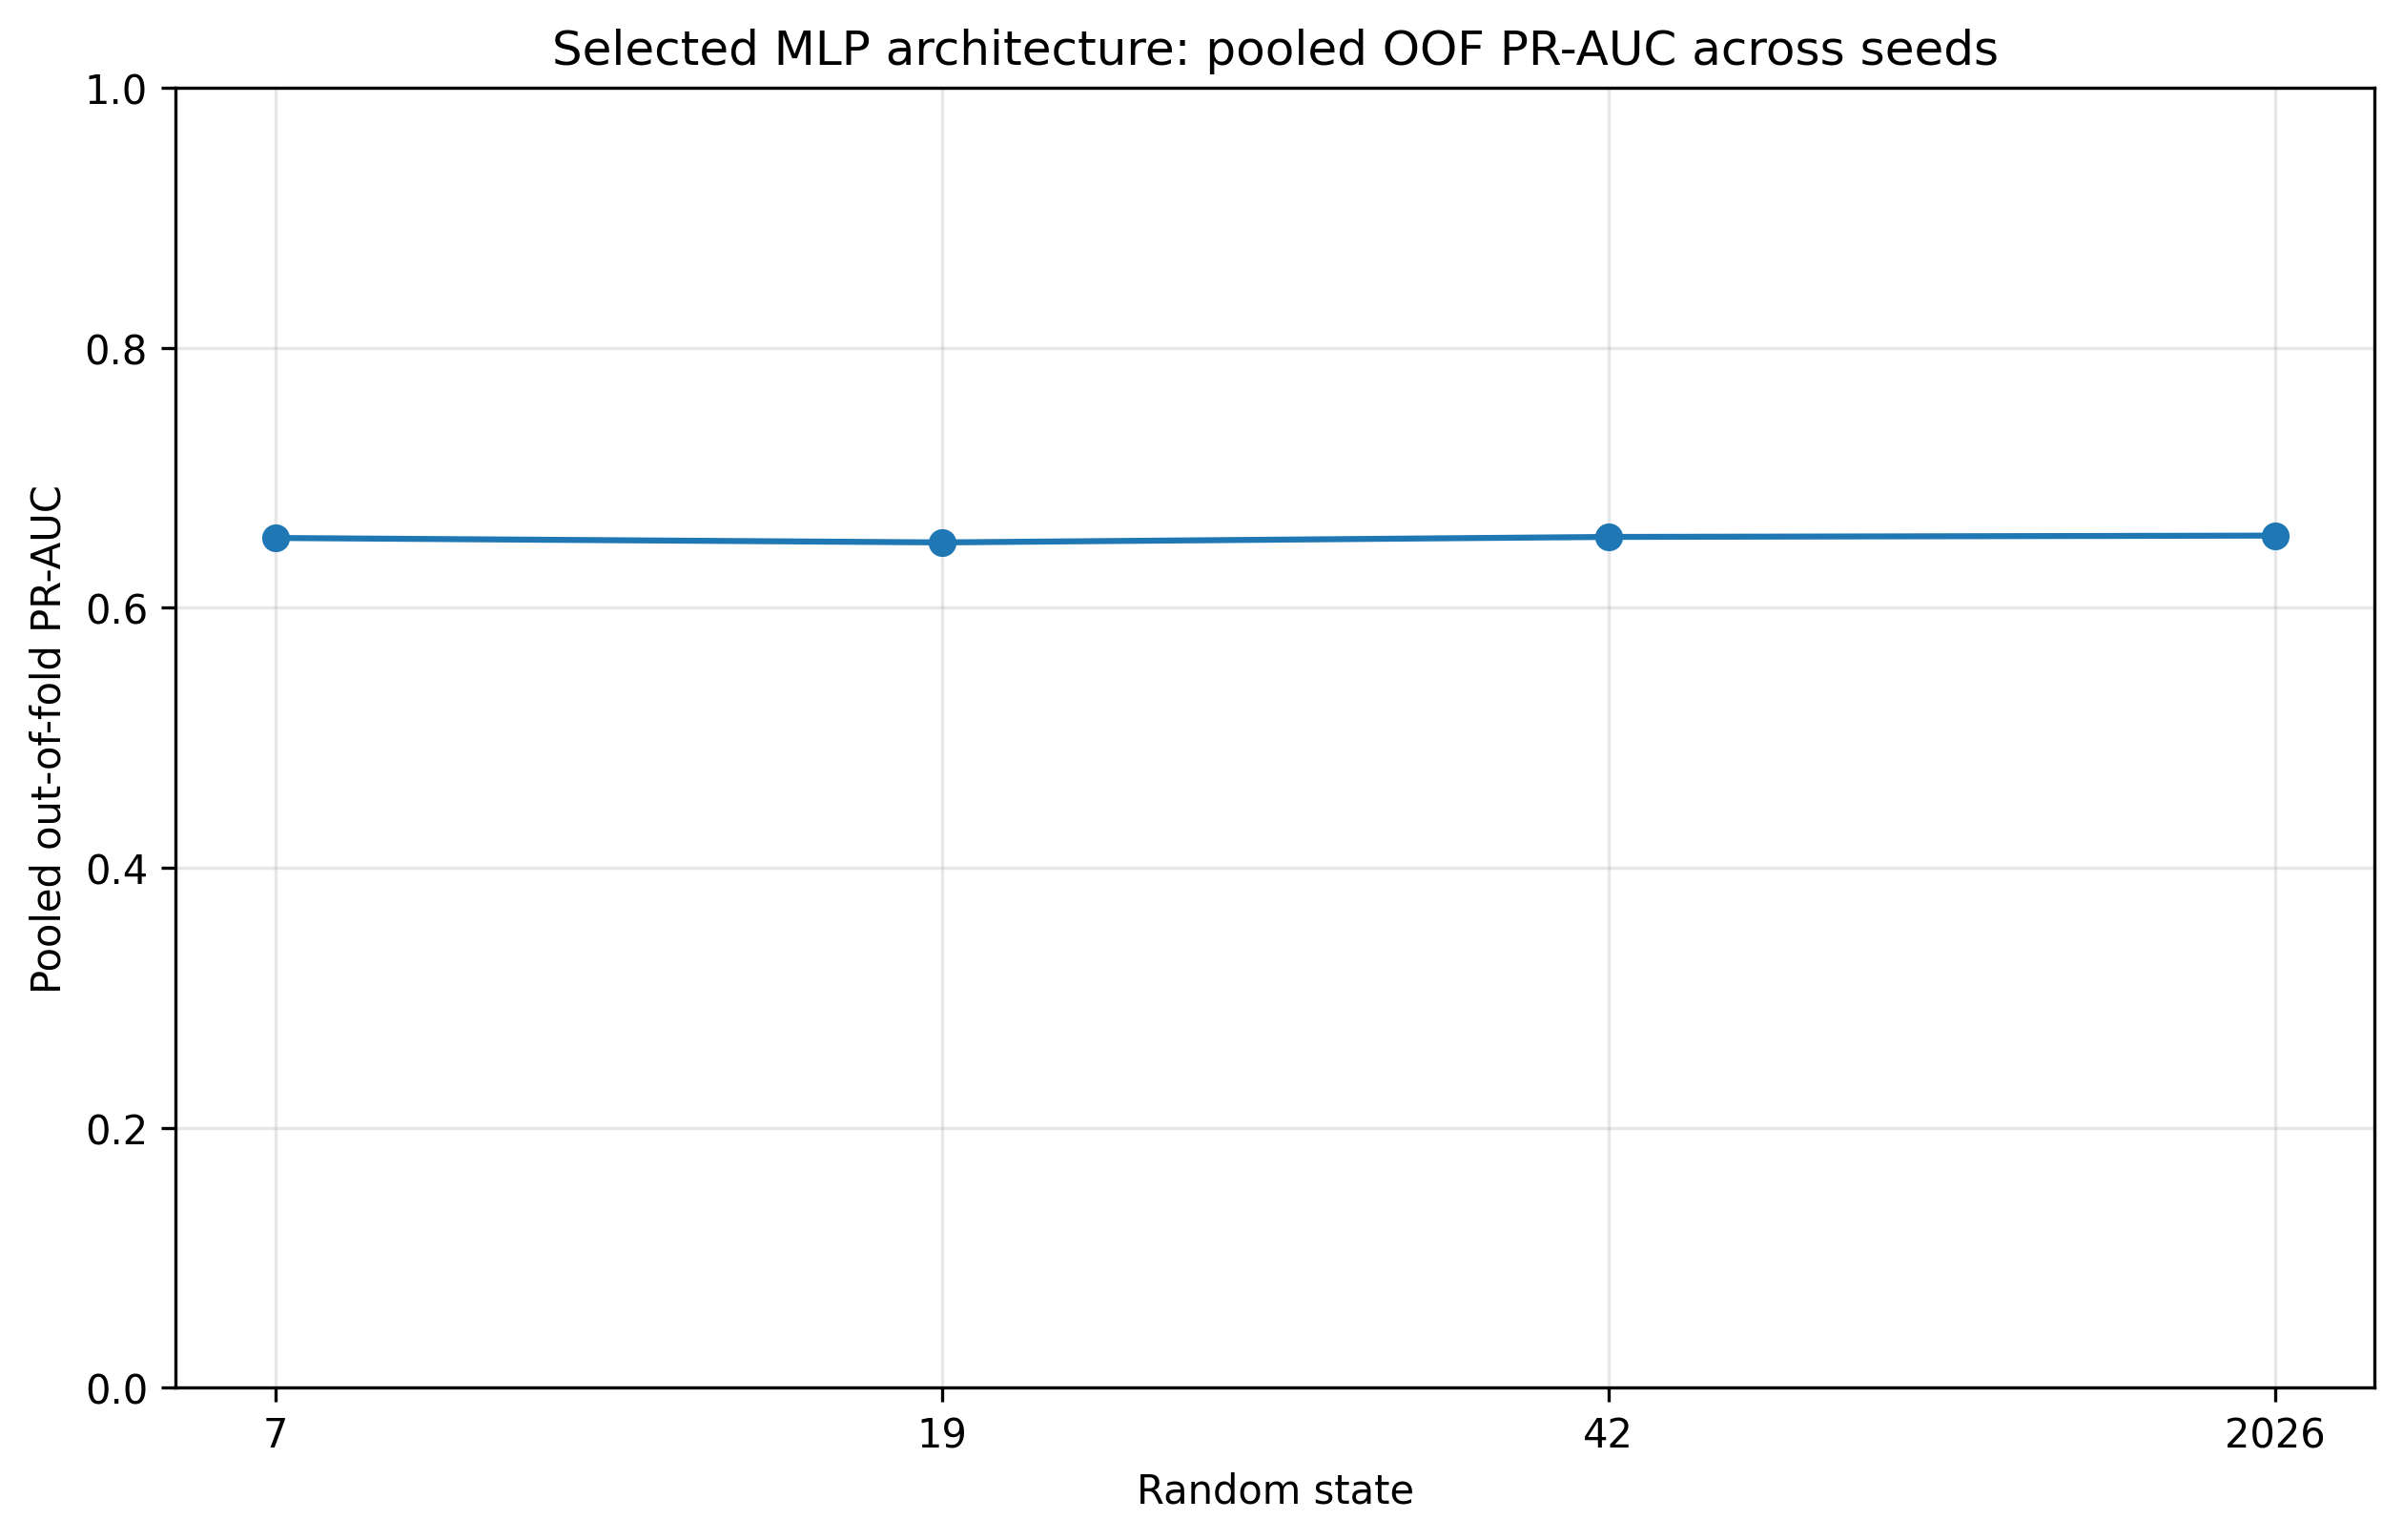
\includegraphics[width=0.82\textwidth]{../figures/mlp_seed_sensitivity_pr_auc.png}
\caption{Pooled OOF PR-AUC of the selected architecture across random seeds}
\label{fig:mlp-seed-sensitivity}
\end{figure}

\subsection{Scoped comparison with representative earlier models}

The MLP is compared with a deliberately limited set of earlier selected configurations. Each reference is reconstructed from the relevant earlier workflow and re-evaluated through fresh training-only cross-validation in the MLP notebook. This supplies comparable pooled OOF predictions and metrics under the same current pipeline and evaluation utilities.

Table~\ref{tab:mlp-model-comparison} is not a final project-wide ranking. It does not include all earlier boosting variants, random forest, RBF SVM, Naive Bayes, or every baseline. It is a local diagnostic that compares the MLP against representative linear, instance-based, single-tree, bagging, margin-based, and strong boosted-tree approaches.

\begin{table}[H]
\centering
\small
\resizebox{\textwidth}{!}{
\begin{tabular}{lrrrrrrrr}
\toprule
Model & Accuracy & Bal. Acc. & Precision & Recall & Specificity & \(F_1\) & ROC-AUC & PR-AUC \\
\midrule
Representative XGBoost & 0.808 & 0.722 & 0.671 & 0.539 & 0.905 & 0.598 & 0.850 & 0.670 \\
Selected bagged trees & 0.800 & 0.705 & 0.662 & 0.504 & 0.907 & 0.572 & 0.846 & 0.662 \\
Selected L2 logistic regression & 0.802 & 0.719 & 0.652 & 0.544 & 0.895 & 0.593 & 0.846 & 0.658 \\
Selected LinearSVC & 0.745 & 0.765 & 0.513 & 0.807 & 0.723 & 0.627 & 0.845 & 0.657 \\
Selected MLP & 0.803 & 0.711 & 0.667 & 0.514 & 0.907 & 0.581 & 0.842 & 0.654 \\
Selected decision tree & 0.789 & 0.701 & 0.624 & 0.514 & 0.888 & 0.564 & 0.824 & 0.628 \\
Selected kNN & 0.792 & 0.722 & 0.617 & 0.571 & 0.872 & 0.593 & 0.836 & 0.628 \\
\bottomrule
\end{tabular}
}
\caption{Scoped pooled out-of-fold comparison of the selected MLP and representative earlier models}
\label{tab:mlp-model-comparison}
\end{table}

In this scoped comparison, the selected MLP is competitive with the selected logistic regression and linear SVM in ranking quality, but it does not exceed the representative XGBoost, bagging, or logistic-regression references in PR-AUC. The MLP and XGBoost have similar default precision and specificity, but the XGBoost reference has higher recall and PR-AUC at its displayed default operating point.

The results therefore do not supply evidence that the MLP's learned nonlinear representation materially improves churn ranking beyond the strong existing approaches. That is a result about the evaluated architecture and search scope, not a claim that neural networks cannot work for churn prediction or tabular data in general.

\begin{figure}[H]
\centering
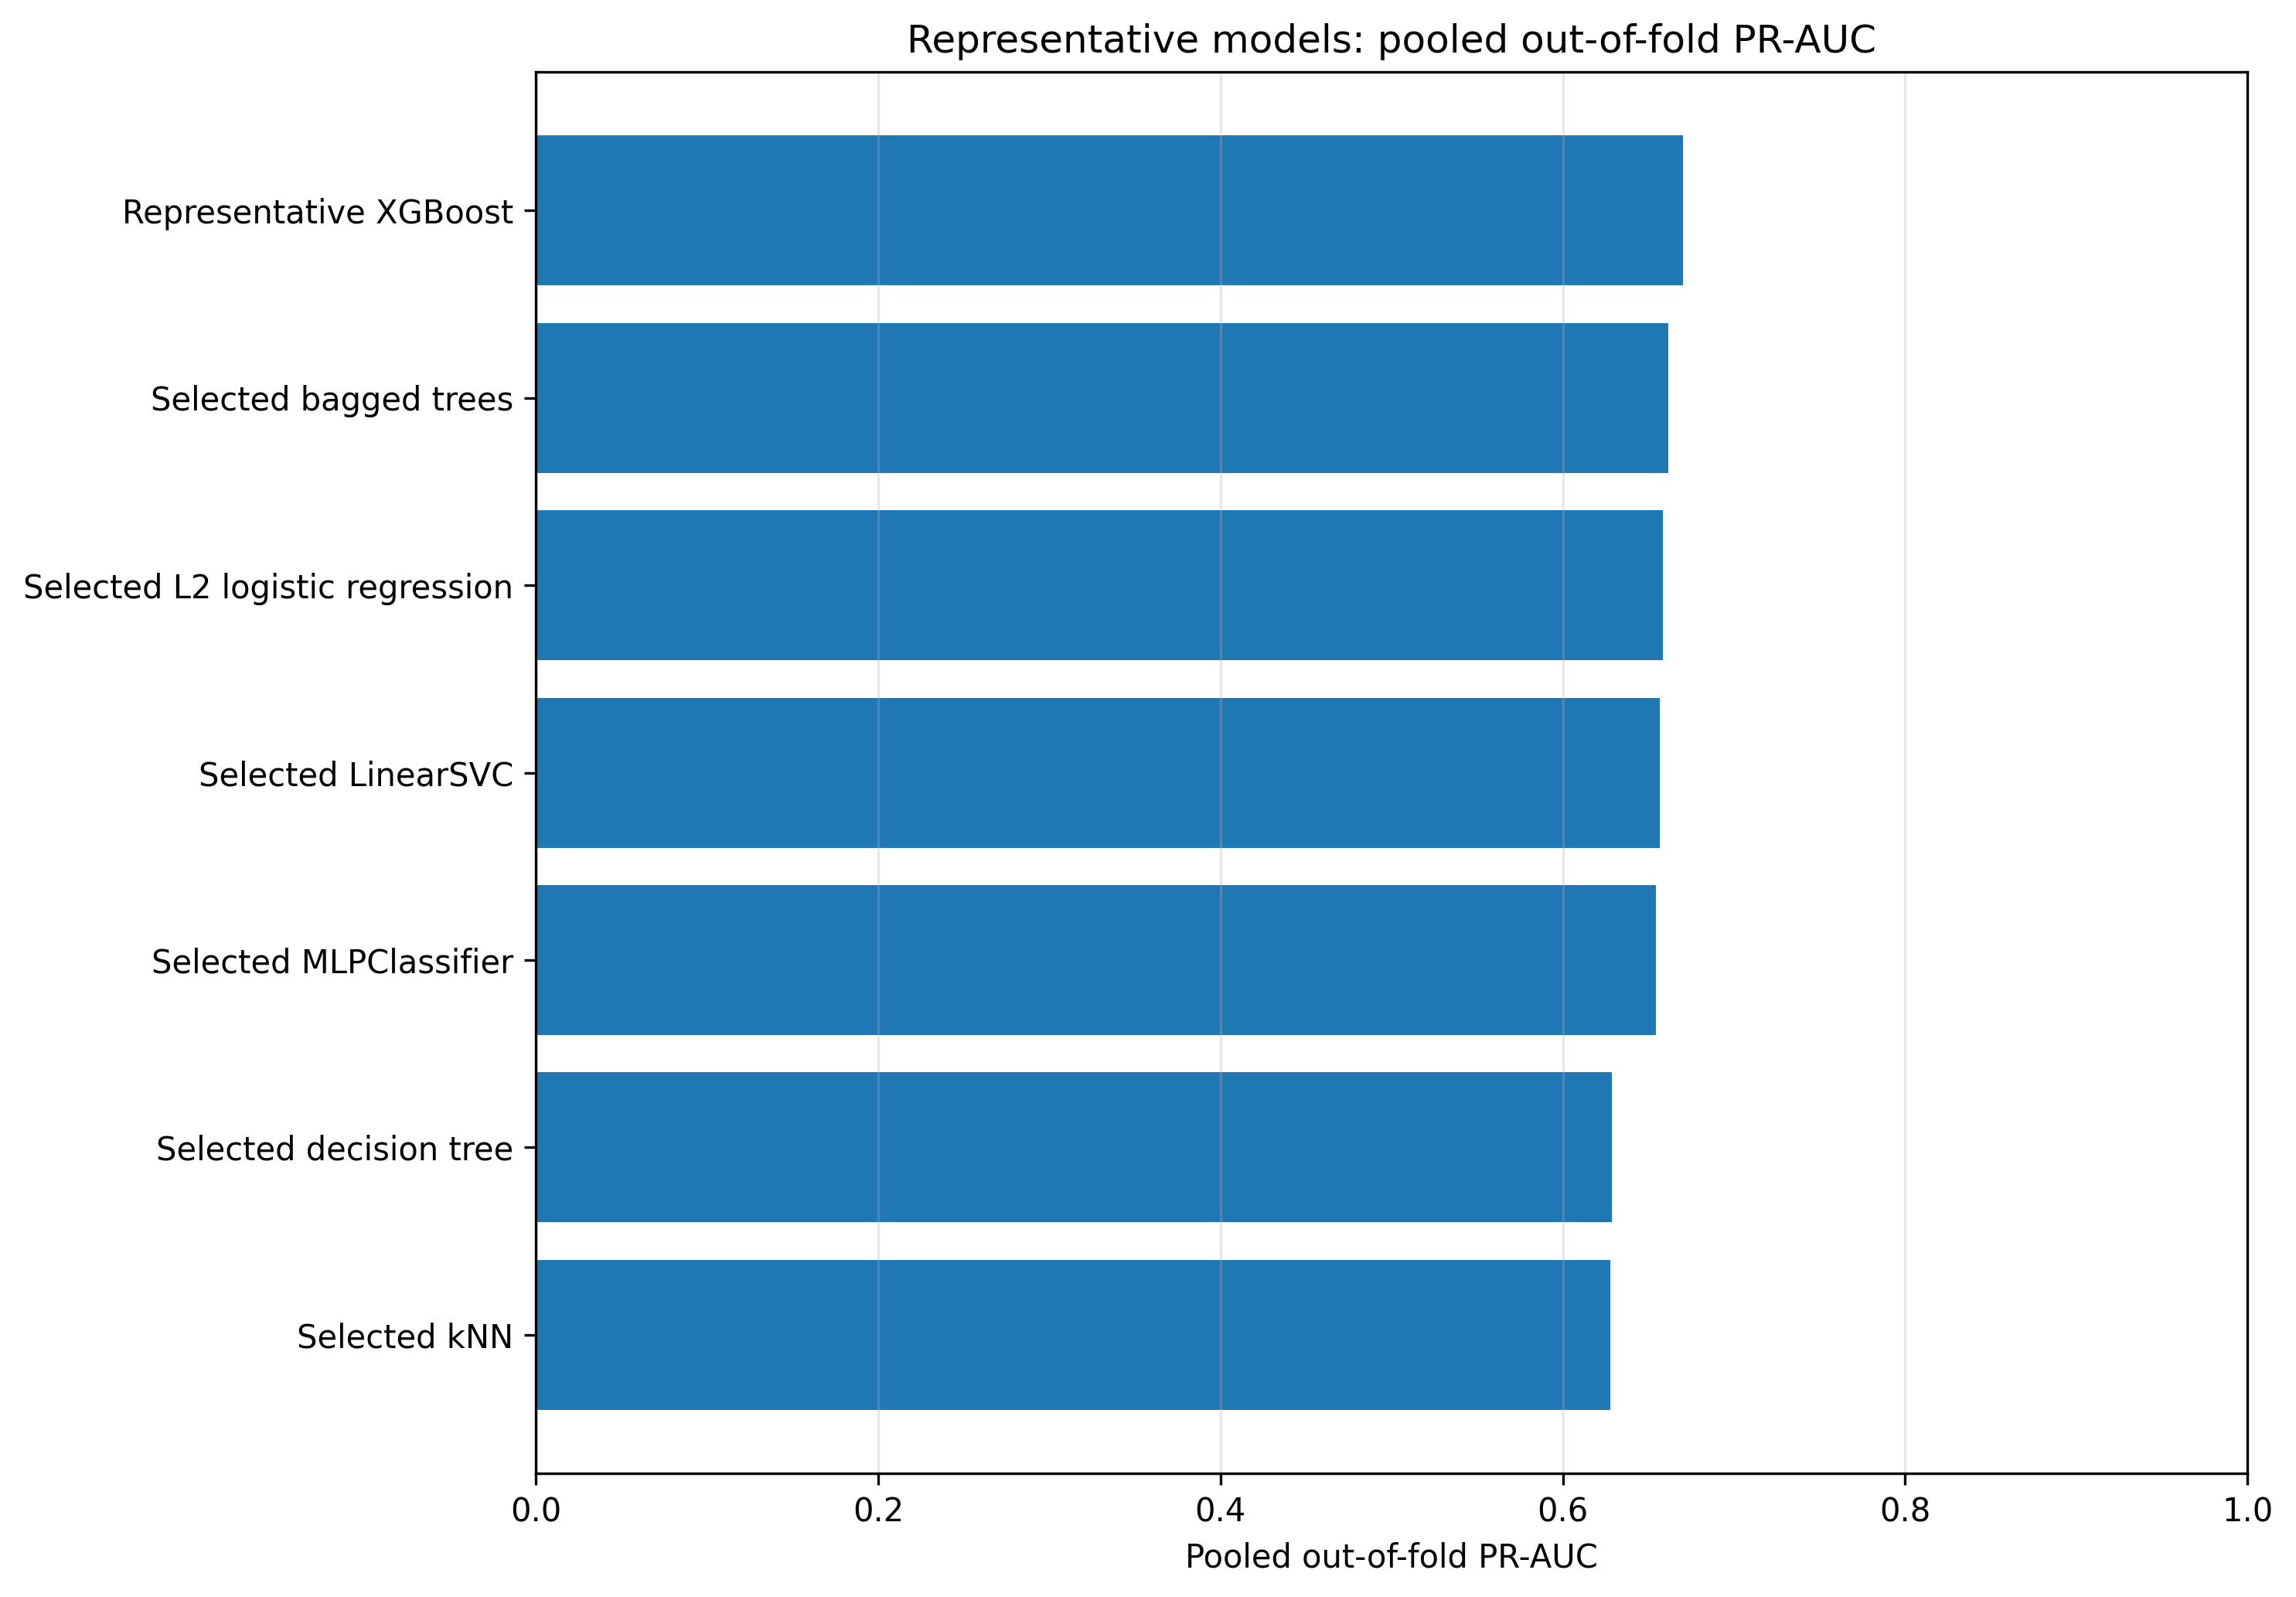
\includegraphics[width=0.90\textwidth]{../figures/mlp_model_comparison_pr_auc.png}
\caption{Selected MLP and representative earlier models: pooled out-of-fold PR-AUC}
\label{fig:mlp-model-comparison}
\end{figure}

\subsection{Conclusion and role in later selection}

The MLP workflow establishes a reproducible neural-network reference for the project: dense fold-safe preprocessing, a compact geometry-aware search, outer-fold PR-AUC selection, early-stopping diagnostics, probability-based threshold analysis, calibration inspection, and seed-sensitivity checks.

The selected \(16\)-unit ReLU MLP is a credible development-stage candidate with useful discrimination and reasonable pooled OOF calibration behaviour. However, the compact search does not demonstrate a clear advantage from additional width, depth, or a \(\tanh\) activation, and the scoped comparison does not show a material ranking advantage over the strongest earlier references.

No final model is selected in this section. A later finalist workflow should define a serious candidate set, compare frozen procedures fairly with appropriate uncertainty assessment, assess calibration where required, choose an operating threshold using retention economics and contact capacity, fit one frozen pipeline on the complete training set, and evaluate the held-out test set once.


\newpage
\section{Final comparison and selection methodology}
\label{sec:final-comparison-methodology}

The preceding sections study individual model families and use development-stage cross-validation to understand their behaviour. Those workflows are intentionally educational and family-specific. They do not by themselves form a fair final comparison because the candidate families differ in their preprocessing requirements, search spaces, computational cost, score semantics, imbalance treatments, and earlier experimental scope.

The final-comparison stage therefore treats each entry as a complete \emph{candidate procedure} rather than as a bare estimator. This section records the methodology that has been implemented for that stage, distinguishes the intended robust comparison from a reduced-cost end-to-end verification run, and defines how future results should be interpreted. The held-out test set remains outside both routes.

\subsection{Candidate procedures rather than estimator names}

For candidate $j$, write the complete procedure as
\[
\mathcal{P}_j
=
\left(
F_j,
S_j,
I_j,
M_j,
\Lambda_j,
\mathcal{A}_j,
R_j
\right),
\]
where $F_j$ is the feature policy, $S_j$ is the feature-selection policy, $I_j$ is the imbalance-treatment policy, $M_j$ is the model family, $\Lambda_j$ is the hyperparameter domain, $\mathcal{A}_j$ is the search and confirmation algorithm, and $R_j$ is the reproducibility and resource contract.

This definition prevents an incomplete comparison such as ``logistic regression versus XGBoost'' from hiding consequential differences. For example, one procedure may use a scaled one-hot representation, another may use native categorical variables, and a third may include fold-internal resampling. Those choices are part of the procedure being evaluated.

The implemented registry contains 26 procedures covering linear, probabilistic, neighbour-based, tree-based, boosting, kernel, neural-network, and advanced tabular model families. The registry includes ridge classification, regularized and spline logistic regression, shrinkage LDA, regularized QDA, k-nearest neighbours, hybrid Naive Bayes, decision trees, Extra Trees, bagging, random forests, balanced random forests, AdaBoost, RUSBoost, standard and histogram-based gradient boosting, XGBoost, LightGBM, CatBoost, Explainable Boosting Machines, linear and RBF support vector machines, multilayer perceptrons, TabNet, FT-Transformer, and TabM.

TabPFN and AutoGluon are not part of the frozen comparison. Their deferral reflects practical package, dependency, model-weight, and computational constraints. It is not a conclusion about their predictive quality.

\subsection{Development and held-out roles}

The clean dataset contains 7,043 observations. A fixed split assigns 5,634 observations to development and 1,409 observations to the held-out test set. All candidate comparison, tuning, threshold analysis, calibration decisions, complementarity analysis, and ensemble construction are development-only activities.

The held-out test set is reserved for one eventual evaluation after one complete procedure has been selected and frozen. Until then, the project makes no final test-performance claim. In particular, the test set is not used to compare individual ensemble members, to revise the threshold, to recalibrate probabilities, or to choose between the robust and reduced-cost routes.

\subsection{Intended robust protocol}

The intended robust comparison is a frozen repeated nested cross-validation protocol over all 5,634 development observations. It uses five stratified outer folds and three repeats. Each of the 26 candidates therefore has 15 outer evaluation tasks, giving 390 candidate-by-outer-split tasks in total.

For outer task $t$ and candidate procedure $\mathcal{P}_j$, the development data are partitioned into an outer-training set $\mathcal{D}^{\mathrm{train}}_{jt}$ and an outer-validation set $\mathcal{D}^{\mathrm{val}}_{jt}$. All search activity occurs inside $\mathcal{D}^{\mathrm{train}}_{jt}$. The outer-validation fold is used exactly once after the internal selection process has finished.

The outer score can be written as
\[
\widehat{M}_{jt}
=
M\left(
\widehat{f}_{jt},
\mathcal{D}^{\mathrm{val}}_{jt}
\right),
\]
where $\widehat{f}_{jt}$ is obtained by tuning and refitting the complete procedure using only $\mathcal{D}^{\mathrm{train}}_{jt}$.

The resulting distribution of outer scores estimates the performance of the complete tuning-and-refit procedure. It does not estimate one globally fixed hyperparameter vector. Different outer tasks may select different feature policies, imbalance treatments, or model hyperparameters, and that variation is itself useful stability evidence.

\subsection{Two-stage internal search}

Each outer-training partition uses a two-stage internal search.

\subsubsection{Stage A: bounded Optuna exploration}

Stage A uses three-fold stratified inner cross-validation. Optuna samples valid combinations from the candidate-specific search space. The sampled configuration may include feature policy, compatible feature selection, compatible imbalance treatment, and model hyperparameters.

The routing layer prevents incoherent combinations before fitting. For example, feature policies and synthetic resampling procedures are not combined when the derived features would no longer be internally consistent with their raw inputs.

Stage A is exploratory. Its purpose is to identify a small set of strong configurations under a bounded and reproducible search budget.

\subsubsection{Stage B: independent confirmation}

Stage B re-evaluates the strongest Stage-A configurations using a separate five-fold stratified confirmation design inside the outer-training partition. This stage reduces dependence on one exploratory split and one noisy Stage-A estimate.

Only after Stage B is complete is one configuration selected. That configuration is refitted on all outer-training observations and evaluated once on the untouched outer-validation fold.

\subsection{Search-budget governance}

Literal equality in the number of trials would not make the comparison fair. A simple linear procedure and a modern tabular neural network have different search dimensionality and runtime. The protocol therefore uses candidate-specific budget lanes that were frozen before robust comparison results were inspected.

\begin{table}[H]
\centering
\caption{Frozen search-budget lanes for the intended robust comparison.}
\label{tab:final-comparison-budget-lanes}
\begin{tabular}{p{3.1cm}p{6.0cm}rrp{2.1cm}}
\toprule
Budget lane & Candidate group & Stage-A trials & Stage-B top $K$ & Profile \\
\midrule
Cheap & C01--C08 and C21 & 36 & 5 & Full \\
Medium & C09--C18 except C19, plus C20, C22, and C23 & 24 & 4 & Full \\
Expensive & C24--C26 & 8 & 2 & Full \\
Runtime-limited & C19 CatBoost & 8 & 2 & CatBoost v2 \\
\bottomrule
\end{tabular}
\end{table}

CatBoost remains included. Runtime calibration showed that unrestricted CatBoost trials were a practical bottleneck, so its frozen profile bounds the number of iterations, depth, learning rate, and L2 leaf regularization. That calibration evidence was used to design a feasible protocol, not to rank or exclude CatBoost.

Changing search budgets after inspecting robust comparison results would create a new protocol version. The same rule applies to candidate inclusion, feature-policy compatibility, imbalance routing, and failure handling.

\subsection{Primary and secondary evidence}

Average precision is the primary ranking metric. It summarizes the precision-recall curve as
\[
\operatorname{AP}
=
\sum_n
\left(R_n-R_{n-1}\right)P_n,
\]
where $P_n$ and $R_n$ are precision and recall at successive score thresholds. Average precision is appropriate for this problem because churn is the minority class and the project is concerned with retrieving likely churners without allowing the majority class to dominate the evaluation.

Secondary evidence includes ROC-AUC, log loss and Brier score when probability outputs are valid, threshold-dependent diagnostics, runtime, warnings, failure states, and selected-parameter stability. The final interpretation should not reduce the comparison to the largest displayed mean AP. Practical equivalence, paired uncertainty, reproducibility, score semantics, computational burden, and implementation complexity also matter.

\subsection{Evidence roles}

Several bounded runs were needed while constructing the comparison infrastructure. Their evidential roles are deliberately separated.

\begin{table}[H]
\centering
\caption{Evidence categories used in the final-comparison workflow.}
\label{tab:final-comparison-evidence-roles}
\begin{tabular}{p{4.2cm}p{9.0cm}}
\toprule
Evidence category & Interpretation \\
\midrule
Implementation admission & Confirms that a candidate can be constructed, fitted, scored, persisted, and resumed under bounded development-only conditions. It does not rank candidates. \\
Runtime evidence & Measures feasibility and informs bounded resource policies. It does not rank or eliminate candidates. \\
Fast-completion development evidence & Exercises the complete end-to-end pipeline with reduced settings. It is useful for procedural verification but weak for substantive comparison. \\
Robust protocol-v2 evidence & Intended repeated nested-CV comparison evidence. It does not yet exist because the full frozen protocol has not been completed. \\
Held-out test evidence & Final evidence for one frozen procedure. It does not yet exist because the test set remains untouched. \\
\bottomrule
\end{tabular}
\end{table}

This terminology prevents a successful smoke test or runtime calibration from being misreported as model-selection evidence.

\subsection{Reduced-cost end-to-end verification}

A separate fast-completion profile was executed to verify that the entire workflow could run successfully before spending the much larger computational budget required by the robust protocol. It retained the complete C01--C26 registry and the same general runner architecture, but deliberately reduced the number of folds, repeats, trials, and confirmations.

\begin{table}[H]
\centering
\caption{Intended robust settings and the reduced-cost verification settings.}
\label{tab:robust-versus-fast-completion}
\begin{tabular}{p{5.6cm}rr}
\toprule
Component & Robust protocol & Verification profile \\
\midrule
Outer folds & 5 & 2 \\
Outer repeats & 3 & 1 \\
Stage-A inner folds & 3 & 2 \\
Stage-B confirmation folds & 5 & 2 \\
Stage-A trials, cheap lane & 36 & 2 \\
Stage-A trials, medium lane & 24 & 2 \\
Stage-A trials, expensive lane & 8 & 2 \\
Stage-B top $K$, cheap lane & 5 & 1 \\
Stage-B top $K$, medium lane & 4 & 1 \\
Stage-B top $K$, expensive lane & 2 & 1 \\
Total outer candidate tasks & 390 & 52 \\
\bottomrule
\end{tabular}
\end{table}

The verification profile answers engineering questions. It tests whether all candidates can pass through one runner, whether artifacts and checksums are correct, whether results can be summarized automatically, whether complete configurations can be reconstructed, whether an ensemble can be refitted and serialized, and whether a guarded one-time test evaluator can be prepared without accessing the test data.

It was not designed to establish which candidate has the strongest and most stable generalization performance. Two outer folds, one repeat, two Optuna trials, and one confirmed configuration per candidate provide only minimal search and uncertainty information. The numerical rankings from this route are therefore provisional fast-completion development evidence, not definitive final-comparison results.

\subsection{Selection after the robust comparison}

Nested cross-validation evaluates a tuning procedure. It does not directly produce one universal final hyperparameter vector. After the robust comparison, the intended downstream sequence is:

\begin{enumerate}
    \item summarize outer-fold metrics, runtime, warnings, failure states, and selected-parameter stability;
    \item identify a leading set using average precision, paired differences, uncertainty, practical equivalence, and operational considerations;
    \item tune leading procedures on all development data using a frozen post-comparison tuning design to obtain concrete executable configurations;
    \item study calibration only for probability-producing leading procedures and only through leakage-safe development predictions;
    \item select a decision threshold from development-only out-of-fold or cross-fitted scores;
    \item evaluate complementarity using leakage-safe out-of-fold predictions;
    \item treat any soft vote, blend, or stack as a separate candidate procedure;
    \item choose one complete procedure, freeze all of its components, and refit it on all 5,634 development observations;
    \item serialize and integrity-check the fitted procedure;
    \item evaluate it once on the untouched held-out test set only after explicit authorization.
\end{enumerate}

The threshold, calibration method, ensemble composition, weights, feature schema, and preprocessing recipe are all part of the final procedure. None may be changed in response to held-out test results.

\subsection{Current execution status}

The reduced-cost route has successfully exercised the complete pipeline through development-data refitting, serialization, reload validation, and preparation of a guarded final-test evaluator. This demonstrates that the implementation is operational.

It does not convert the reduced-cost ranking into robust scientific evidence. The robust repeated nested-CV protocol remains the intended methodology for strong candidate-comparison claims and may be run later without touching the held-out test set.

A procedure frozen inside the fast-completion route should therefore be interpreted as frozen within that verification route. Because the held-out test remains untouched, the future robust development-only comparison can still provide the stronger evidence used to choose the procedure that eventually receives the single final test evaluation.

\subsection{Reporting implications}

Until the robust comparison is completed, appropriate descriptions include ``implemented candidate procedure,'' ``runtime evidence,'' ``reduced-cost end-to-end verification,'' ``provisional fast-route selection,'' and ``held-out test not yet evaluated.''

Descriptions such as ``final winner,'' ``statistically superior,'' ``robust benchmark result,'' or ``final unbiased performance'' would overstate the available evidence. The project can document the completed engineering workflow now, while reserving strong comparative and final performance claims for the appropriate future evidence.


\newpage
\begin{thebibliography}{9}

\bibitem{ml-preprocessing}
Vrije Universiteit Amsterdam Machine Learning course notes.
\textit{Data pre-processing, Part 1: Missing values and outliers}.
Used for the principles of not taking data at face value, distinguishing missing feature values from missing target labels, considering the production setting, and distinguishing corrupted values from natural extreme observations.

\bibitem{ml-evaluation}
Vrije Universiteit Amsterdam Machine Learning course notes.
\textit{Model Evaluation, Part 1: Experiments}.
Used for train/validation/test discipline, cross-validation, the distinction between true performance and estimated performance, and the principle that held-out test data should not be reused during model development.

\bibitem{dl-tools}
Vrije Universiteit Amsterdam Deep Learning course notes.
\textit{Tools of the trade}.
Used for the practical evaluation principles that test-set size controls metric uncertainty, validation data is used for development and hyperparameter tuning, test data is reserved for final reporting, leakage must be actively avoided, baselines should be used during development, hyperparameter tuning should balance performance and simplicity, and fair comparisons require comparable tuning effort.

\end{thebibliography}

\end{document}
